\documentclass{article}
\usepackage[utf8]{inputenc}
\usepackage{amsmath}
\usepackage{fullpage}
\usepackage{hyperref}
\usepackage{tikz}
\usepackage{pgfplots}
\usepackage{float}
\usepackage{caption}
\usetikzlibrary{shapes.geometric, arrows, positioning}

\tikzstyle{start} = [rectangle, rounded corners, minimum width=3cm, minimum height=1cm,text centered, draw=black]
\tikzstyle{process} = [rectangle, minimum width=3cm, minimum height=1cm, text centered, draw=black]
\tikzstyle{arrow} = [thick,->,>=stealth]

\title{Reunderstand PSOLA}
\author{Kanru Hua}
\date{December 2015}

\begin{document}

\maketitle

\section{Introduction}

PSOLA (Pitch Synchronous OverLap and Add)\cite{moulines}, an algorithm able to change the duration or shift the pitch of speech signals, invented around 1990 (arguably) by France Telecom, remains being \textit{the} most widely used speech modification algorithm as of 2015. Staying in time-domain from the beginning to its end, this incredibly simple algorithm outputs speech at pretty good quality and blazingly fast speed. Given such a pleasant compromise between complexity, speed and quality, no wonder those top-tier softwares (e.g. Melodyne\textsuperscript{\textregistered} and Auto-Tune\textsuperscript{\textregistered}) in music production industry are using PSOLA as their `secret' weapon to conquer the market; no wonder those top-tier universities all over the world more or less put PSOLA in their speech processing courses.

What leaves me wondering is: seems like there's always a blind spot in all tutorials, slides and papers about PSOLA. In a few sentences they tell you something like,
\footnote{A much more detailed yet easy-to-understand video introduction can be found on Professor Simon King's website, \url{http://www.speech.zone/td-psola-the-hard-way/}}
\begin{quote} PSOLA basically marks the ``epochs'' (some call them Glottal Closure Instants or Instants of Significant Excitation), puts a bunch of 2-period-long hanning windows on these epochs, cuts the signal into pieces, and finally adds the pieces back together (at some different epoch positions determined by pitch and time stretch). \end{quote}
Now you can clutch onto your favourite editor, implement the whole thing in a few hundred lines. They've taught you \textit{how does it work}, but they hide the more intriguing fact from you - \textit{what does this mean?}, or they themselves either don't know what PSOLA does in frequency domain.

The goal of this quite informal article is to fill in the blank, i.e., to gain a deep understanding of PSOLA, discover a few interesting properties, and see how to ultimately improve the algorithm using these properties.

\section{PSOLA as a Source-Filter Model}

You may have heard of this a hundred times, but for completeness I still have to mention it again. The very classical source-filter model of speech production is an acoustic simplification of the actual, physical process of passing quasi-periodic volume velocity flow through vocal-tract and going out from lip. After making a great deal of (stupid) assumptions such as the organs are stationary during phonation and the whole process is linear (which of course is not true), the speech production process can be expressed as a pulse train\footnote{A pulse train is a bunch of Dirac Delta functions shifted and added together.} going through a chain of cascaded filters resembling each organ,

\begin{center}
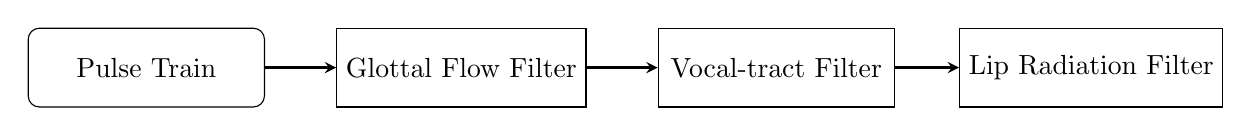
\begin{tikzpicture}[node distance=4cm]
\node (ptrain) [start] {Pulse Train};
\node (glottal) [process, right of=ptrain] {Glottal Flow Filter};
\node (vtract) [process, right of=glottal] {Vocal-tract Filter};
\node (liprad) [process, right of=vtract] {Lip Radiation Filter};
\draw [arrow] (ptrain) -- (glottal);
\draw [arrow] (glottal) -- (vtract);
\draw [arrow] (vtract) -- (liprad);
\end{tikzpicture}
\end{center}

An even simpler model is achieved by combining the three filters into one,

\bigskip

\begin{center}
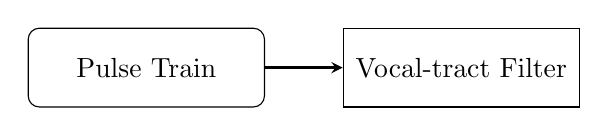
\begin{tikzpicture}[node distance=4cm]
\node (ptrain) [start] {Pulse Train};
\node (vtract) [process, right of=ptrain] {Vocal-tract Filter};
\draw [arrow] (ptrain) -- (vtract);
\end{tikzpicture}
\end{center}

which suggests that your vocal fold suddenly bursts open and closes again in no time, being an even more ridiculous assumption. Afterall, only by making these assumptions the model becomes tractable, and can be implemented on a digital computer. Some recent researches are trying to narrow down the assumptions, but that's out of the scope for our discussion.

Back to PSOLA, consider the process of extracting lots of pieces, each covering 2 periods of speech signal, and adding them back. This perfectly fits into the simplified source-filter model, \textbf{where the vocal-tract filter's impulse responses, slowly varying along time, are the pieces extracted}. In time-domain, filtering corresponds to convolution, and convolution with a pulse train is equivalent to shifting and adding the impulse response onto each pulse (or epoch) position.

This further implies that the analysis procedure - marking the epochs and windowing the signal - is to \textbf{deconvolve} the speech signal into separated source (pulse train) and filter (vocal-tract filter) component!

\section{PSOLA from a Frequency Domain Perspective}

Now let's take a step further by examining PSOLA and the underlying source-filter model in frequency domain. An interesting way of doing this is to insert a pair of Fourier Transform and Inverse Fourier Transform\footnote{When dealing with discrete signals, one can use Discrete Time Fourier Transform, or Discrete Fourier Transform in a more practical sense. Note that we're doing the transform for each windowed piece, in a way similar to STFT, but being pitch-synchronous.} into the middle,

\begin{center}
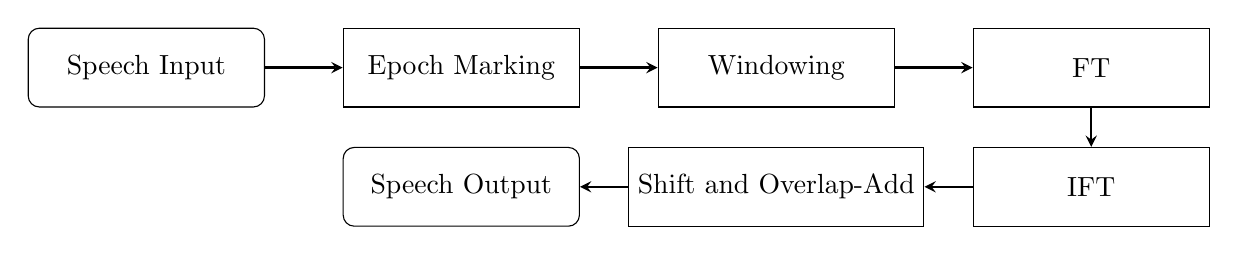
\begin{tikzpicture}[node distance=4cm]
\node (input) [start] {Speech Input};
\node (epoch) [process, right of=input] {Epoch Marking};
\node (window) [process, right of=epoch] {Windowing};
\node (ft) [process, right of=window] {FT};
\node (ift) [process, below = 0.5 of ft] {IFT};
\node (shift-ola) [process, left of=ift] {Shift and Overlap-Add};
\node (output) [start, left of=shift-ola] {Speech Output};
\draw [arrow] (input) -- (epoch);
\draw [arrow] (epoch) -- (window);
\draw [arrow] (window) -- (ft);
\draw [arrow] (ft) -- (ift);
\draw [arrow] (ift) -- (shift-ola);
\draw [arrow] (shift-ola) -- (output);
\end{tikzpicture}
\end{center}

This is actually a variant known as FD-PSOLA (Frequency-Domain PSOLA), which allows you to carry out frequency domain filtering between FT and IFT blocks in the above flowchart. Without such filtering, obviously the insertion of FT/IFT doesn't change anything in the result. But from now on we can split the algorithm into two parts: the analysis part,

\begin{center}
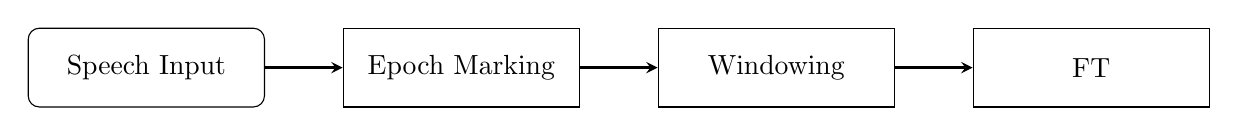
\begin{tikzpicture}[node distance=4cm]
\node (input) [start] {Speech Input};
\node (epoch) [process, right of=input] {Epoch Marking};
\node (window) [process, right of=epoch] {Windowing};
\node (ft) [process, right of=window] {FT};
\draw [arrow] (input) -- (epoch);
\draw [arrow] (epoch) -- (window);
\draw [arrow] (window) -- (ft);
\end{tikzpicture}
\end{center}

and the synthesis part,

\begin{center}
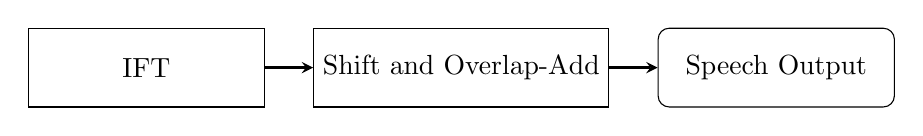
\begin{tikzpicture}[node distance=4cm]
\node (ift) [process] {IFT};
\node (shift-ola) [process, right of=ift] {Shift and Overlap-Add};
\node (output) [start, right of=shift-ola] {Speech Output};
\draw [arrow] (ift) -- (shift-ola);
\draw [arrow] (shift-ola) -- (output);
\end{tikzpicture}
\end{center}

In the following we tackle down each part respectively. It's good to start with the analysis part.

\subsection{Analysis Subprocess}

We shall first review the concept of narrowband and wideband spectrum. These two terms have multiple definitions regarding to different contexts. In speech processing, a narrowband spectrum displays well-resolved harmonic structure (for voiced speech) while a wideband spectrum only shows a rough contour as if joining all harmonics by a smooth curve.

PSOLA's window is only two periods long so we can safely assume that the fundamental frequency is constant around each analysis instant. Since the analysis window fades to zero on both sides, it doesn't matter if the pitch outside of the window changes or not, so we can still consider the constant frequency and infinite length pulse train as the excitation signal. The Fourier Transform of such a pulse train is also a pulse train in frequency domain, exhibiting a harmonic structure,

\begin{align}
\sum_n \delta(t - nT_0) \leftrightarrow \frac{2\pi}{T_0} \sum_n \delta(\omega - \frac{2\pi n}{T_0})
\end{align}

When filtered by the vocal-tract filter it becomes,

\begin{align}
v(t) \ast \sum_n \delta(t - nT_0) \leftrightarrow \frac{2\pi}{T_0} \sum_n V(\omega) \delta(\omega - \frac{2\pi n}{T_0})
\end{align}

where $v(t)$ and $V(\omega)$ are the impulse response and frequency response of the vocal-tract filter, respectively. This is a very, very narrow-band spectrum since each harmonic is infinitely narrow and super nicely resolved.

Now consider the effect of windowing. Modulating (multiplying) the infinite length signal by a finite length window is to convolve the spectrum of two signals in frequency domain. When one of the spectrums is a pulse train, this becomes shifting and adding the window's spectrum onto each pulse. Here the vocal-tract frequency response is reduced to a vector of phasors $V_n$ since equation (2) is only non-zero on each harmonic,

\begin{align}
w(t) \left(v(t) \ast \sum_n \delta(t - nT_0) \right) \leftrightarrow \frac{2\pi}{T_0} \sum_n V_n W(\omega - \frac{2\pi n}{T_0})
\end{align}

The magical power behind PSOLA lies in the use of 2-period-long hanning window in its analysis part. It has a main-lobe radius of $\frac{2\pi}{T_0}$ radians\footnote{Professor Julius O. Smith has written a nice book\cite{smith} covering some topics on window properties.}, which exactly fills in the gap between neighbouring harmonics ($\omega - \frac{2\pi n}{T_0}$ in equation (1)-(3)). This guarantees that harmonics are not resolved and the spectrum is hence wideband. In summary, PSOLA's analysis subprocess is a wideband spectrum estimation method\footnote{Some call this ``Spectral Envelope Estimation" but it mostly refers to magnitude response estimation only.} whose output is smooth in both magnitude and phase.

\subsection{Synthesis Subprocess}

The synthesis part simply consists of two linear operations: inverse Fourier Transform, and shift and overlap-add. We can swap the order of execution by first shifting and adding in frequency domain and then transforming to time domain. Given the estimated wideband spectrum $V(\omega)$, the output $y(t)$ is expressed in a manner similar to equation (1)-(3). Again, we can assume the fundamental being constant because it hardly changes within an analysis frame.

\begin{align}
y(t)      &= \mathrm{F}^{-1} \{ \sum_n V(\omega) e^{j n \omega T_0} \} \\
Y(\omega) &= V(\omega) \sum_n e^{j n \omega T_0} \\
\hat Y(\omega) &= V(\omega) \underset{N \to \infty}{\mathrm{lim}} \frac{1}{N} \sum^N_n e^{j n \omega T_0} = V(\omega) |_{\omega = \frac{2\pi n}{T_0}}
\end{align}

The right hand side of equation (5) is the summation of many harmonically-related complex sinusoids. When $\omega \neq \frac{2\pi n}{T_0}$, the complex values cancel out to give a zero, otherwise it pops up to infinity. By normalizing $Y(\omega)$ by the range of summation, the normalized output spectrum equals to $V(\omega)$ at harmonic frequencies. In other words, $V(\omega)$ is subsampled at harmonic frequencies,  generating a narrowband spectrum $\hat Y(\omega)$.

\subsection{Preliminary Conclusions}

So far we've examined both the analysis and synthesis part. By cascading them together, PSOLA first \emph{implicitly} estimates an array of wideband spectrum from the input signal, at each analysis instant synchronized to period; then it \emph{implicitly} reconstructs narrowband spectrum by subsampling the wideband spectrum at a modified fundamental frequency. Without pitch modification (i.e. time-scale modification only), the narrowband spectrum can be perfectly preserved throughout the process.

In the context of source-filter model, the wideband spectrum estimated from the input represents the vocal-tract transfer function. Note that not only magnitude but also phase response of the vocal-tract are estimated, being different from most spectral envelope estimators (e.g. STRAIGHT, SEEVOC) which only consider the magnitude component. However, PSOLA has a critical flaw that the vocal-tract impulse response is time-limited to 2 periods. When the pitch is shifted down by less than half, the separation between two pulses becomes longer than the impulse response, and a small region in the middle is left blank.

\section{Interference Issues and Epoch Marking}

In section 3.1, equation (3) assumes that both the pulse train and the window are centered at time zero. In a more realistic case, we need to add a time shift representing the location of epoch or analysis instant.

\begin{align}
w(t) \left(v(t) \ast \sum_n \delta(t - nT_0 - \Delta T) \right) \leftrightarrow \frac{2\pi}{T_0} \sum_n e^{-j\Delta T \omega} V_n W(\omega - \frac{2\pi n}{T_0})
\end{align}

Note that $V_n$ is a phasor which follows the definition $V_n = a_n e^{j\theta_n}$; the spectrum of a symmetric window is real. Thus the phase component for each harmonic in the summation is $\theta_n - \Delta T \omega$.

Here arises an interference problem in the wideband spectrum: when neighbouring harmonics have different phases, the overlapping spectral content in the middle is attenuated. This is depicted in Figure 1 where a 9-period speech signal is synthesized from the wideband spectrum (red) at 300Hz. In the left figure the synthetic signal is windowed at a local extrema; in the right figure the window is shifted by 20\% of the period. A new wideband spectrum (green) is calculated from the windowed signal. In the right figure we can find a few valleys in inter-harmonic regions spanning from 1kHz to 4.5kHz.

This example shows that epoch marking has a critical effect on the quality of wideband spectrum, and the undesirable valleys can be prevented, to some extent, by centering the window at a local maximum of absolute value of the signal. Indeed, time-domain peak picking is a commonly used epoch marking method for PSOLA\footnote{The PSOLA implementation in Praat uses local extrema based epoch marking (``Sound - To manipulation...").}.

\begin{figure}[H]
\centering
\scalebox{.65}{% This file was created by matlab2tikz.
%
%The latest updates can be retrieved from
%  http://www.mathworks.com/matlabcentral/fileexchange/22022-matlab2tikz-matlab2tikz
%where you can also make suggestions and rate matlab2tikz.
%
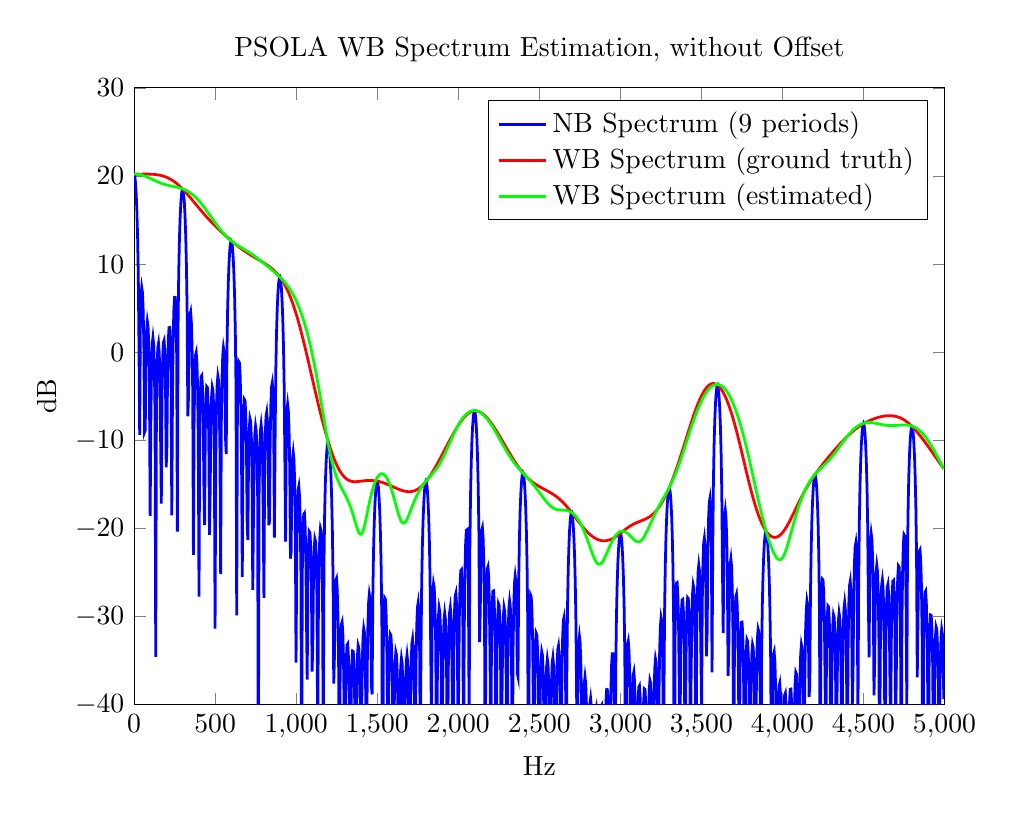
\begin{tikzpicture}

\begin{axis}[%
width=4.052in,
height=3.084in,
at={(0.68in,0.416in)},
scale only axis,
xmin=0,
xmax=5000,
xlabel={Hz},
ymin=-40,
ymax=30,
ylabel={dB},
axis background/.style={fill=white},
title={PSOLA WB Spectrum Estimation, without Offset},
legend style={legend cell align=left,align=left,legend plot pos=left,draw=black}
]
\addplot [color=blue,solid,line width=1.0pt]
  table[row sep=crcr]{%
0	20.1998112835222\\
4.306640625	19.9630253688939\\
8.61328125	19.2360845575318\\
12.919921875	17.9633168361555\\
17.2265625	16.0268836225403\\
21.533203125	13.180537695682\\
25.83984375	8.82254699381025\\
30.146484375	0.700132969808097\\
34.453125	-9.38373028135972\\
38.759765625	2.98659328058475\\
43.06640625	6.33169751815378\\
47.373046875	7.30266913618077\\
51.6796875	6.77667164223539\\
55.986328125	4.80429815421497\\
60.29296875	0.750174864059773\\
64.599609375	-9.06739986575636\\
68.90625	-8.84633812663461\\
73.212890625	-0.448845833559547\\
77.51953125	2.5403005536744\\
81.826171875	3.47160202128536\\
86.1328125	2.92848316932768\\
90.439453125	0.823665076872224\\
94.74609375	-3.79589942490457\\
99.052734375	-18.5756773333599\\
103.359375	-7.93671108111667\\
107.666015625	-1.59488202972874\\
111.97265625	0.938574790851837\\
116.279296875	1.65231303930877\\
120.5859375	0.911077829630306\\
124.892578125	-1.52749587117764\\
129.19921875	-7.11592771881383\\
133.505859375	-34.5722812401772\\
137.8125	-6.61373585025094\\
142.119140625	-1.57112851524897\\
146.42578125	0.545998657477225\\
150.732421875	1.00846814542794\\
155.0390625	0.00753024427498389\\
159.345703125	-2.88396851268621\\
163.65234375	-9.97838634972832\\
167.958984375	-17.1927718041873\\
172.265625	-4.78035058609264\\
176.572265625	-0.638401029402439\\
180.87890625	1.12216069547664\\
185.185546875	1.33907375557166\\
189.4921875	0.0523509699633727\\
193.798828125	-3.40616894653224\\
198.10546875	-13.0783607136449\\
202.412109375	-10.8149063853367\\
206.71875	-2.21399351427716\\
211.025390625	1.2932326952125\\
215.33203125	2.78023534109459\\
219.638671875	2.79677833190986\\
223.9453125	1.23710570621143\\
228.251953125	-2.90986314652361\\
232.55859375	-18.5287229748842\\
236.865234375	-5.07437946200521\\
241.171875	1.68146492127122\\
245.478515625	4.82865651916769\\
249.78515625	6.2251383823794\\
254.091796875	6.21700298464575\\
258.3984375	4.54902151417185\\
262.705078125	-0.316094354876905\\
267.01171875	-20.3631341734267\\
271.318359375	3.0575325482516\\
275.625	9.27891427842231\\
279.931640625	12.9384014511283\\
284.23828125	15.3605744062789\\
288.544921875	16.9768834776396\\
292.8515625	17.9772307831562\\
297.158203125	18.4540713750781\\
301.46484375	18.4483724573271\\
305.771484375	17.9654551343891\\
310.078125	16.9768328564373\\
314.384765625	15.4096529514292\\
318.69140625	13.1137629249197\\
322.998046875	9.76421522356002\\
327.3046875	4.48366650833135\\
331.611328125	-7.28779593916486\\
335.91796875	-4.96268408957308\\
340.224609375	1.99861917064307\\
344.53125	4.24016109828537\\
348.837890625	4.56604715190631\\
353.14453125	3.47389454839626\\
357.451171875	0.821822316752798\\
361.7578125	-4.4793399264641\\
366.064453125	-22.9871894100464\\
370.37109375	-7.92767303445529\\
374.677734375	-2.4009077695411\\
378.984375	-0.342290696274627\\
383.291015625	-0.0312863801554487\\
387.59765625	-1.16210097745387\\
391.904296875	-4.03150884435551\\
396.2109375	-10.3064811168369\\
400.517578125	-27.7454720012042\\
404.82421875	-8.96041617777776\\
409.130859375	-4.50057833605844\\
413.4375	-2.76654864977965\\
417.744140625	-2.64331898403537\\
422.05078125	-3.98848799706377\\
426.357421875	-7.29656530604883\\
430.6640625	-15.2784849930523\\
434.970703125	-19.6280359003298\\
439.27734375	-8.99724258837361\\
443.583984375	-5.32514630847748\\
447.890625	-3.90870070723117\\
452.197265625	-4.01131670320744\\
456.50390625	-5.63872381985393\\
460.810546875	-9.55198582122405\\
465.1171875	-20.7180942624329\\
469.423828125	-15.7930568669292\\
473.73046875	-8.16917574371243\\
478.037109375	-5.08890608921028\\
482.34375	-3.95112449656558\\
486.650390625	-4.27886302677546\\
490.95703125	-6.22662574650125\\
495.263671875	-10.9467752816124\\
499.5703125	-31.3720854955781\\
503.876953125	-12.3005026495531\\
508.18359375	-6.31416655720202\\
512.490234375	-3.66153375393449\\
516.796875	-2.73342069721742\\
521.103515625	-3.24679935077833\\
525.41015625	-5.52163956819098\\
529.716796875	-11.3416106283318\\
534.0234375	-25.1884263224476\\
538.330078125	-7.88815132235102\\
542.63671875	-2.83702992295379\\
546.943359375	-0.390317992662059\\
551.25	0.506453767531607\\
555.556640625	-0.0166482969133403\\
559.86328125	-2.47547139389485\\
564.169921875	-9.79720344227454\\
568.4765625	-11.5585700714678\\
572.783203125	-0.260917670788041\\
577.08984375	4.80216728799505\\
581.396484375	7.96660497742971\\
585.703125	10.0888756045376\\
590.009765625	11.4884644993177\\
594.31640625	12.3134403650122\\
598.623046875	12.6356434402504\\
602.9296875	12.4829286915673\\
607.236328125	11.8494208999965\\
611.54296875	10.6934370617096\\
615.849609375	8.92126187582147\\
620.15625	6.34018611552969\\
624.462890625	2.51060127598473\\
628.76953125	-3.93058726765696\\
633.076171875	-29.8765921370504\\
637.3828125	-7.22073387554979\\
641.689453125	-2.58802074239123\\
645.99609375	-1.08406020592237\\
650.302734375	-1.22451821675793\\
654.609375	-2.76748144168745\\
658.916015625	-6.07369842266098\\
663.22265625	-13.0703615125042\\
667.529296875	-25.4888922745812\\
671.8359375	-10.7681475759189\\
676.142578125	-6.80085219175046\\
680.44921875	-5.37724854639443\\
684.755859375	-5.51878242265869\\
689.0625	-7.1315311122338\\
693.369140625	-10.7845917295229\\
697.67578125	-19.6906547805135\\
701.982421875	-21.331947444522\\
706.2890625	-12.0232587584064\\
710.595703125	-8.70507389456911\\
714.90234375	-7.52962795903941\\
719.208984375	-7.85076038400367\\
723.515625	-9.72012802481867\\
727.822265625	-14.0032074625755\\
732.12890625	-26.9681252466484\\
736.435546875	-18.9683572216046\\
740.7421875	-12.0946118990068\\
745.048828125	-9.31566283462937\\
749.35546875	-8.40778630849761\\
753.662109375	-8.96009418001901\\
757.96875	-11.1765633942772\\
762.275390625	-16.3715606156391\\
766.58203125	-50.4097779235462\\
770.888671875	-16.649390269191\\
775.1953125	-11.2182619719317\\
779.501953125	-8.87541873477621\\
783.80859375	-8.21734155257196\\
788.115234375	-9.01485145668904\\
792.421875	-11.6480762232233\\
796.728515625	-18.1820357938765\\
801.03515625	-27.8814763418916\\
805.341796875	-13.7899449945592\\
809.6484375	-9.29777925877496\\
813.955078125	-7.28269765023121\\
818.26171875	-6.82222429053385\\
822.568359375	-7.84092958267098\\
826.875	-10.9426873551596\\
831.181640625	-19.6363187515666\\
835.48828125	-19.2147076680975\\
839.794921875	-9.70840578203416\\
844.1015625	-5.77334921409505\\
848.408203125	-3.89682282661396\\
852.71484375	-3.46440523501345\\
857.021484375	-4.5384695767372\\
861.328125	-8.0257594005086\\
865.634765625	-21.0448365225365\\
869.94140625	-10.0975056717451\\
874.248046875	-2.195712077007\\
878.5546875	2.03661305204502\\
882.861328125	4.77327991030721\\
887.16796875	6.60322091770327\\
891.474609375	7.76851277988212\\
895.78125	8.38504242800249\\
900.087890625	8.50728188270865\\
904.39453125	8.15087262548289\\
908.701171875	7.2982955639766\\
913.0078125	5.89269374756126\\
917.314453125	3.81429303836856\\
921.62109375	0.812655230261074\\
925.927734375	-3.72703921020973\\
930.234375	-12.1406550808728\\
934.541015625	-21.4830175679408\\
938.84765625	-9.79456922700259\\
943.154296875	-6.68408706564325\\
947.4609375	-5.91921294684327\\
951.767578125	-6.65127897304316\\
956.07421875	-8.84128343273207\\
960.380859375	-13.1459599848905\\
964.6875	-23.4280461085132\\
968.994140625	-22.709719872331\\
973.30078125	-14.7526519311194\\
977.607421875	-12.0393831716497\\
981.9140625	-11.3674018549286\\
986.220703125	-12.1729621553081\\
990.52734375	-14.554974476215\\
994.833984375	-19.4978085436939\\
999.140625	-35.2394625173893\\
1003.447265625	-23.7992519007091\\
1007.75390625	-17.8583238819868\\
1012.060546875	-15.6433421617602\\
1016.3671875	-15.237997396714\\
1020.673828125	-16.2922529627976\\
1024.98046875	-19.0614079921665\\
1029.287109375	-25.0486132711531\\
1033.59375	-49.0489298744527\\
1037.900390625	-24.8089499761534\\
1042.20703125	-20.1642092960551\\
1046.513671875	-18.3960011512\\
1050.8203125	-18.2748293831415\\
1055.126953125	-19.6214733178922\\
1059.43359375	-22.8791188728092\\
1063.740234375	-30.4530193089661\\
1068.046875	-37.1668211819933\\
1072.353515625	-25.5193434711999\\
1076.66015625	-21.7657194537968\\
1080.966796875	-20.3597785467106\\
1085.2734375	-20.4901021210194\\
1089.580078125	-22.127753296442\\
1093.88671875	-25.9629911891354\\
1098.193359375	-36.246288353504\\
1102.5	-33.579043475189\\
1106.806640625	-25.4932347862979\\
1111.11328125	-22.3449523604847\\
1115.419921875	-21.1911146165028\\
1119.7265625	-21.5004356503055\\
1124.033203125	-23.3902174237449\\
1128.33984375	-27.9048897074595\\
1132.646484375	-44.7102230597605\\
1136.953125	-30.2833775016506\\
1141.259765625	-23.9262840157376\\
1145.56640625	-21.0912950068375\\
1149.873046875	-19.9863411636628\\
1154.1796875	-20.279564559475\\
1158.486328125	-22.2395319531199\\
1162.79296875	-27.4586537681424\\
1167.099609375	-45.5842743246826\\
1171.40625	-24.2089204093871\\
1175.712890625	-18.2949510731541\\
1180.01953125	-14.8851512980094\\
1184.326171875	-12.691793179793\\
1188.6328125	-11.2912626612358\\
1192.939453125	-10.4963177591208\\
1197.24609375	-10.2156703212552\\
1201.552734375	-10.4090021409064\\
1205.859375	-11.0714974932495\\
1210.166015625	-12.2322431141108\\
1214.47265625	-13.9650961185263\\
1218.779296875	-16.4223268513851\\
1223.0859375	-19.9344917157253\\
1227.392578125	-25.4005568635528\\
1231.69921875	-37.6231868881101\\
1236.005859375	-34.6680737629009\\
1240.3125	-27.994825560824\\
1244.619140625	-25.8959841344629\\
1248.92578125	-25.683528706939\\
1253.232421875	-26.8777749478328\\
1257.5390625	-29.6326456080537\\
1261.845703125	-35.0734362938085\\
1266.15234375	-54.8514097573601\\
1270.458984375	-38.2663073589712\\
1274.765625	-32.8892469234498\\
1279.072265625	-30.8979252819675\\
1283.37890625	-30.6323479254595\\
1287.685546875	-31.8008987748611\\
1291.9921875	-34.7145473825549\\
1296.298828125	-41.1009369688574\\
1300.60546875	-56.9684224491254\\
1304.912109375	-39.3767009237428\\
1309.21875	-34.9724360950563\\
1313.525390625	-33.2423355395328\\
1317.83203125	-33.1077098181897\\
1322.138671875	-34.4384930600509\\
1326.4453125	-37.7474979121764\\
1330.751953125	-45.8624166843514\\
1335.05859375	-49.4140706504964\\
1339.365234375	-39.0528066719654\\
1343.671875	-35.3738318088744\\
1347.978515625	-33.9175038023049\\
1352.28515625	-33.9714153074006\\
1356.591796875	-35.5531776289137\\
1360.8984375	-39.4494940305821\\
1365.205078125	-50.9154625398585\\
1369.51171875	-45.1326337947302\\
1373.818359375	-37.5949215377083\\
1378.125	-34.4764153065035\\
1382.431640625	-33.2801179057106\\
1386.73828125	-33.5465690198466\\
1391.044921875	-35.442810828673\\
1395.3515625	-40.1602796322515\\
1399.658203125	-62.3297224810393\\
1403.96484375	-40.9954863426594\\
1408.271484375	-35.0323309007632\\
1412.578125	-32.3354466062052\\
1416.884765625	-31.3511525962668\\
1421.19140625	-31.8101434649747\\
1425.498046875	-34.046959405141\\
1429.8046875	-39.9115330777737\\
1434.111328125	-52.4321846741827\\
1438.41796875	-35.9521220254251\\
1442.724609375	-30.9035515648031\\
1447.03125	-28.4187098024568\\
1451.337890625	-27.4766849716494\\
1455.64453125	-27.9592258329553\\
1459.951171875	-30.4009573586294\\
1464.2578125	-37.8600226117026\\
1468.564453125	-38.8379538202033\\
1472.87109375	-27.7690945672026\\
1477.177734375	-22.699252507885\\
1481.484375	-19.4999587165494\\
1485.791015625	-17.3350331009931\\
1490.09765625	-15.8904446411636\\
1494.404296875	-15.0202858544826\\
1498.7109375	-14.6538325756486\\
1503.017578125	-14.763980876241\\
1507.32421875	-15.3572926702582\\
1511.630859375	-16.4763102847611\\
1515.9375	-18.2161636858893\\
1520.244140625	-20.7725504988485\\
1524.55078125	-24.593560318074\\
1528.857421875	-31.0824962855242\\
1533.1640625	-60.4598649948022\\
1537.470703125	-33.9555491987503\\
1541.77734375	-29.3921165970853\\
1546.083984375	-27.8964933617719\\
1550.390625	-28.0350725088891\\
1554.697265625	-29.5790381622938\\
1559.00390625	-32.9040089035676\\
1563.310546875	-40.0097778309555\\
1567.6171875	-51.3457965177724\\
1571.923828125	-37.3078224679822\\
1576.23046875	-33.3955540299073\\
1580.537109375	-31.9889397035259\\
1584.84375	-32.1406957438218\\
1589.150390625	-33.7684943613522\\
1593.45703125	-37.461074618364\\
1597.763671875	-46.5793964602232\\
1602.0703125	-47.5026766593959\\
1606.376953125	-38.4446636874249\\
1610.68359375	-35.1711415105569\\
1614.990234375	-34.0147420882645\\
1619.296875	-34.3504665004912\\
1623.603515625	-36.2413845084006\\
1627.91015625	-40.5813332190181\\
1632.216796875	-54.0586877968533\\
1636.5234375	-45.1511662193199\\
1640.830078125	-38.4103418998207\\
1645.13671875	-35.6618951858327\\
1649.443359375	-34.765945852533\\
1653.75	-35.3272437045274\\
1658.056640625	-37.5623193933281\\
1662.36328125	-42.8305154979651\\
1666.669921875	-104.975649309368\\
1670.9765625	-42.7176261684347\\
1675.283203125	-37.3554006713557\\
1679.58984375	-35.0202604587396\\
1683.896484375	-34.3553669793566\\
1688.203125	-35.1442114329868\\
1692.509765625	-37.7822420781882\\
1696.81640625	-44.4144001495545\\
1701.123046875	-53.1280943956726\\
1705.4296875	-39.557383620042\\
1709.736328125	-35.0795141923781\\
1714.04296875	-33.0373838420722\\
1718.349609375	-32.537675104167\\
1722.65625	-33.5163269255627\\
1726.962890625	-36.5977631423763\\
1731.26953125	-45.4597924187348\\
1735.576171875	-44.2477100992935\\
1739.8828125	-34.8845159778428\\
1744.189453125	-30.9041931763623\\
1748.49609375	-28.9515049463273\\
1752.802734375	-28.4320019136335\\
1757.109375	-29.4194416822271\\
1761.416015625	-32.8506957161765\\
1765.72265625	-46.3693479059954\\
1770.029296875	-34.2808557895966\\
1774.3359375	-26.3628142786716\\
1778.642578125	-22.012212267465\\
1782.94921875	-19.1298878090504\\
1787.255859375	-17.1389723439664\\
1791.5625	-15.8011055204505\\
1795.869140625	-15.0019564760371\\
1800.17578125	-14.6878788442319\\
1804.482421875	-14.8438126989631\\
1808.7890625	-15.4878698935034\\
1813.095703125	-16.6777739056355\\
1817.40234375	-18.5349570979253\\
1821.708984375	-21.3138581276861\\
1826.015625	-25.6425256313867\\
1830.322265625	-33.9442357631557\\
1834.62890625	-42.1597878516606\\
1838.935546875	-30.6691442082378\\
1843.2421875	-27.3358130752316\\
1847.548828125	-26.3048331016152\\
1851.85546875	-26.7550654832247\\
1856.162109375	-28.6590153040817\\
1860.46875	-32.6953363038248\\
1864.775390625	-42.9213312966232\\
1869.08203125	-41.1489301883569\\
1873.388671875	-33.0534286338037\\
1877.6953125	-30.0312904603135\\
1882.001953125	-29.0189732567229\\
1886.30859375	-29.4721500512705\\
1890.615234375	-31.5017047311995\\
1894.921875	-36.1247461605529\\
1899.228515625	-52.2578341102143\\
1903.53515625	-39.257415060976\\
1907.841796875	-33.0260082349903\\
1912.1484375	-30.4289480557643\\
1916.455078125	-29.6194221961028\\
1920.76171875	-30.262464662772\\
1925.068359375	-32.6271824401265\\
1929.375	-38.2703220889431\\
1933.681640625	-59.1053156735768\\
1937.98828125	-36.7723546280088\\
1942.294921875	-31.7508918386798\\
1946.6015625	-29.5519867758319\\
1950.908203125	-28.9868558169204\\
1955.21484375	-29.8891711266675\\
1959.521484375	-32.7195201566249\\
1963.828125	-39.9823078447383\\
1968.134765625	-45.4239550221179\\
1972.44140625	-33.7083735260088\\
1976.748046875	-29.5421199220567\\
1981.0546875	-27.6922591596885\\
1985.361328125	-27.373922383357\\
1989.66796875	-28.5702431157747\\
1993.974609375	-31.9952016286193\\
1998.28125	-42.1255368344246\\
2002.587890625	-38.2680387530637\\
2006.89453125	-29.9185333260343\\
2011.201171875	-26.3667689335384\\
2015.5078125	-24.7931589442721\\
2019.814453125	-24.6852642225431\\
2024.12109375	-26.1727921058266\\
2028.427734375	-30.3354640337953\\
2032.734375	-47.7581845535017\\
2037.041015625	-31.523196112068\\
2041.34765625	-24.876446907335\\
2045.654296875	-21.6822384967924\\
2049.9609375	-20.2118969681157\\
2054.267578125	-20.1480821852721\\
2058.57421875	-21.7734467574225\\
2062.880859375	-26.7385880562228\\
2067.1875	-42.708700428162\\
2071.494140625	-22.4378312304649\\
2075.80078125	-16.268347544036\\
2080.107421875	-12.5651348389637\\
2084.4140625	-10.0764442180625\\
2088.720703125	-8.38683419825366\\
2093.02734375	-7.31216979394629\\
2097.333984375	-6.7627752268266\\
2101.640625	-6.69940453707979\\
2105.947265625	-7.11814163178113\\
2110.25390625	-8.04903307402283\\
2114.560546875	-9.56726083744622\\
2118.8671875	-11.8275001917677\\
2123.173828125	-15.1662322951206\\
2127.48046875	-20.5049129293377\\
2131.787109375	-32.9100769045871\\
2136.09375	-29.0395782303147\\
2140.400390625	-22.3989845730526\\
2144.70703125	-20.216793504205\\
2149.013671875	-19.9144194854456\\
2153.3203125	-21.0295818274495\\
2157.626953125	-23.7281883666489\\
2161.93359375	-29.1728089073116\\
2166.240234375	-50.3589227083544\\
2170.546875	-31.9000210182524\\
2174.853515625	-26.5942818768441\\
2179.16015625	-24.6152615654851\\
2183.466796875	-24.3604339158489\\
2187.7734375	-25.5516873228188\\
2192.080078125	-28.5139349482537\\
2196.38671875	-35.0378142404274\\
2200.693359375	-49.554029092935\\
2205	-33.0309637153544\\
2209.306640625	-28.7545838765739\\
2213.61328125	-27.1184416954249\\
2217.919921875	-27.0782027772328\\
2222.2265625	-28.5153083048277\\
2226.533203125	-31.9605190444566\\
2230.83984375	-40.3646109213481\\
2235.146484375	-43.2906400808699\\
2239.453125	-33.3493502412746\\
2243.759765625	-29.8439687825046\\
2248.06640625	-28.5387648225808\\
2252.373046875	-28.7439277105515\\
2256.6796875	-30.4880394813397\\
2260.986328125	-34.5832900040212\\
2265.29296875	-46.5990097123003\\
2269.599609375	-40.1606439750171\\
2273.90625	-32.9316172930479\\
2278.212890625	-30.0067637592205\\
2282.51953125	-28.9867621626858\\
2286.826171875	-29.4284880457928\\
2291.1328125	-31.5108852154617\\
2295.439453125	-36.4652544837721\\
2299.74609375	-61.2066593100598\\
2304.052734375	-37.2553728178305\\
2308.359375	-31.5458712771851\\
2312.666015625	-29.035643615261\\
2316.97265625	-28.2236888746236\\
2321.279296875	-28.8538076898643\\
2325.5859375	-31.2750064812107\\
2329.892578125	-37.4064015955918\\
2334.19921875	-48.9209090606158\\
2338.505859375	-33.3616871250172\\
2342.8125	-28.5190609187449\\
2347.119140625	-26.1964438496571\\
2351.42578125	-25.405220410786\\
2355.732421875	-26.0387521508391\\
2360.0390625	-28.6507573839285\\
2364.345703125	-36.4386239401824\\
2368.65234375	-36.8163491943689\\
2372.958984375	-26.1301111832324\\
2377.265625	-21.2175341126822\\
2381.572265625	-18.142535171817\\
2385.87890625	-16.0884878695765\\
2390.185546875	-14.7466392148609\\
2394.4921875	-13.9731773329578\\
2398.798828125	-13.6984663538312\\
2403.10546875	-13.8961398044653\\
2407.412109375	-14.5734375108637\\
2411.71875	-15.7737572192914\\
2416.025390625	-17.5936551150677\\
2420.33203125	-20.2318764371414\\
2424.638671875	-24.1452343518514\\
2428.9453125	-30.7789852175617\\
2433.251953125	-66.4019714005567\\
2437.55859375	-33.4074736682387\\
2441.865234375	-28.987962257558\\
2446.171875	-27.5724058903906\\
2450.478515625	-27.7760166309201\\
2454.78515625	-29.3830933938643\\
2459.091796875	-32.7846132055057\\
2463.3984375	-40.0568646178564\\
2467.705078125	-50.4272465723129\\
2472.01171875	-37.0441163688065\\
2476.318359375	-33.2257025076207\\
2480.625	-31.8728563210116\\
2484.931640625	-32.0688774796672\\
2489.23828125	-33.7433360633389\\
2493.544921875	-37.5054889999806\\
2497.8515625	-46.8750563107116\\
2502.158203125	-47.1081249117755\\
2506.46484375	-38.3111303772849\\
2510.771484375	-35.1047564400771\\
2515.078125	-33.9902587211159\\
2519.384765625	-34.3636517375759\\
2523.69140625	-36.2998882110528\\
2527.998046875	-40.7225502599253\\
2532.3046875	-54.7896259723685\\
2536.611328125	-44.9542860085908\\
2540.91796875	-38.3705088203463\\
2545.224609375	-35.6840327972781\\
2549.53125	-34.8350881342123\\
2553.837890625	-35.4442094639198\\
2558.14453125	-37.7410973198588\\
2562.451171875	-43.1324081573405\\
2566.7578125	-76.1903742019872\\
2571.064453125	-42.7385826262528\\
2575.37109375	-37.5061328476314\\
2579.677734375	-35.2482304782899\\
2583.984375	-34.6533440754984\\
2588.291015625	-35.5179554296034\\
2592.59765625	-38.2536050675571\\
2596.904296875	-45.0898161596529\\
2601.2109375	-52.9737074838001\\
2605.517578125	-39.9911606084764\\
2609.82421875	-35.6541297611105\\
2614.130859375	-33.7228341105146\\
2618.4375	-33.3326144968328\\
2622.744140625	-34.431166579502\\
2627.05078125	-37.6644405259101\\
2631.357421875	-46.891886904165\\
2635.6640625	-45.0820004386549\\
2639.970703125	-36.0577487702048\\
2644.27734375	-32.2516534925379\\
2648.583984375	-30.456208457312\\
2652.890625	-30.0967095589726\\
2657.197265625	-31.2586116410841\\
2661.50390625	-34.9101754842159\\
2665.810546875	-49.2903420505588\\
2670.1171875	-36.2939839737482\\
2674.423828125	-28.6721665421373\\
2678.73046875	-24.5341727714305\\
2683.037109375	-21.8517686865512\\
2687.34375	-20.0597004739853\\
2691.650390625	-18.9230923415622\\
2695.95703125	-18.3289537736819\\
2700.263671875	-18.2242397382096\\
2704.5703125	-18.5942402492394\\
2708.876953125	-19.4574264964143\\
2713.18359375	-20.8721590766889\\
2717.490234375	-22.9613131717362\\
2721.796875	-25.9831650620963\\
2726.103515625	-30.5791306822711\\
2730.41015625	-39.2645015623732\\
2734.716796875	-46.8868912081727\\
2739.0234375	-36.0683906140521\\
2743.330078125	-33.0340079398172\\
2747.63671875	-32.2705155956855\\
2751.943359375	-32.983141617458\\
2756.25	-35.1555622573567\\
2760.556640625	-39.4886561707437\\
2764.86328125	-50.2490157418892\\
2769.169921875	-47.9977935954882\\
2773.4765625	-40.3451102434544\\
2777.783203125	-37.6128311072676\\
2782.08984375	-36.8675804163977\\
2786.396484375	-37.5835646475393\\
2790.703125	-39.8832746168773\\
2795.009765625	-44.8172531012501\\
2799.31640625	-62.0877268366828\\
2803.623046875	-48.0597883289766\\
2807.9296875	-42.1796095214999\\
2812.236328125	-39.850498316468\\
2816.54296875	-39.2913922967276\\
2820.849609375	-40.181558693505\\
2825.15625	-42.8034887160782\\
2829.462890625	-48.7692269644519\\
2833.76953125	-67.6710190603224\\
2838.076171875	-47.3425535143462\\
2842.3828125	-42.6081152478516\\
2846.689453125	-40.6435224122418\\
2850.99609375	-40.2984757190075\\
2855.302734375	-41.4186741297192\\
2859.609375	-44.4817140564073\\
2863.916015625	-52.0960084439547\\
2868.22265625	-56.939576564549\\
2872.529296875	-45.7727514113484\\
2876.8359375	-41.8325635694862\\
2881.142578125	-40.1717222817265\\
2885.44921875	-40.0303520492362\\
2889.755859375	-41.402890184059\\
2894.0625	-45.0269874700971\\
2898.369140625	-55.6237059565789\\
2902.67578125	-51.1512579611434\\
2906.982421875	-43.106376082989\\
2911.2890625	-39.7154560459105\\
2915.595703125	-38.2746719849119\\
2919.90234375	-38.2893844680599\\
2924.208984375	-39.9011946186281\\
2928.515625	-44.2258187205749\\
2932.822265625	-62.9494539894544\\
2937.12890625	-45.20416419073\\
2941.435546875	-38.7302720219932\\
2945.7421875	-35.6264854791727\\
2950.048828125	-34.2243062951739\\
2954.35546875	-34.220291840784\\
2958.662109375	-35.9110167472255\\
2962.96875	-41.0075527373224\\
2967.275390625	-55.4321085229669\\
2971.58203125	-36.3630249381074\\
2975.888671875	-30.2626760136278\\
2980.1953125	-26.5734731289619\\
2984.501953125	-24.078095669258\\
2988.80859375	-22.3689574290012\\
2993.115234375	-21.2649081185316\\
2997.421875	-20.6778419447195\\
3001.728515625	-20.5695944891797\\
3006.03515625	-20.9371997656282\\
3010.341796875	-21.8117530474599\\
3014.6484375	-23.2698926232029\\
3018.955078125	-25.4688899689393\\
3023.26171875	-28.7514749790093\\
3027.568359375	-34.0626002178549\\
3031.875	-46.7567933837926\\
3036.181640625	-42.0140647141125\\
3040.48828125	-35.4435329180323\\
3044.794921875	-33.2047814029782\\
3049.1015625	-32.8229357294588\\
3053.408203125	-33.853055362479\\
3057.71484375	-36.4734686098061\\
3062.021484375	-41.885772554196\\
3066.328125	-64.8001384985309\\
3070.634765625	-44.0256507891853\\
3074.94140625	-38.7036744803229\\
3079.248046875	-36.6377587337947\\
3083.5546875	-36.2807343098695\\
3087.861328125	-37.3681605304621\\
3092.16796875	-40.2395008626668\\
3096.474609375	-46.75175834256\\
3100.78125	-59.8863713418095\\
3105.087890625	-44.1156968253799\\
3109.39453125	-39.7750411909474\\
3113.701171875	-38.0305600785413\\
3118.0078125	-37.8714321790394\\
3122.314453125	-39.1908994264135\\
3126.62109375	-42.5385019620826\\
3130.927734375	-50.996269243384\\
3135.234375	-53.0517320032755\\
3139.541015625	-43.2478666730607\\
3143.84765625	-39.6420742745509\\
3148.154296875	-38.2063564403349\\
3152.4609375	-38.27326957514\\
3156.767578125	-39.8828059491262\\
3161.07421875	-43.8738874749665\\
3165.380859375	-56.1615792805698\\
3169.6875	-48.7221387693273\\
3173.994140625	-41.4716201956768\\
3178.30078125	-38.4104877986395\\
3182.607421875	-37.232334849377\\
3186.9140625	-37.5104322603686\\
3191.220703125	-39.4361475502621\\
3195.52734375	-44.2826065316391\\
3199.833984375	-72.3506328331899\\
3204.140625	-44.3239033174075\\
3208.447265625	-38.508211668137\\
3212.75390625	-35.8248824814399\\
3217.060546875	-34.8237049563143\\
3221.3671875	-35.261700656896\\
3225.673828125	-37.5028864137859\\
3229.98046875	-43.5392487927682\\
3234.287109375	-53.7643667312617\\
3238.59375	-38.6700987201614\\
3242.900390625	-33.6625174686423\\
3247.20703125	-31.1321120878291\\
3251.513671875	-30.1216839461902\\
3255.8203125	-30.5363663846188\\
3260.126953125	-32.949699653548\\
3264.43359375	-40.7078270498552\\
3268.740234375	-40.1211212656282\\
3273.046875	-29.4343011190198\\
3277.353515625	-24.3111897390541\\
3281.66015625	-20.9948615767834\\
3285.966796875	-18.6877990173082\\
3290.2734375	-17.0865656035023\\
3294.580078125	-16.0495393873017\\
3298.88671875	-15.5082678115976\\
3303.193359375	-15.437209479094\\
3307.5	-15.8443631517951\\
3311.806640625	-16.7740590742392\\
3316.11328125	-18.3243586101523\\
3320.419921875	-20.6971585827839\\
3324.7265625	-24.3582545035936\\
3329.033203125	-30.7966632455941\\
3333.33984375	-87.898308503967\\
3337.646484375	-32.5023850324611\\
3341.953125	-27.8882052865314\\
3346.259765625	-26.2187432694613\\
3350.56640625	-26.1560297487135\\
3354.873046875	-27.4972729398102\\
3359.1796875	-30.6490528995852\\
3363.486328125	-37.7680234425667\\
3367.79296875	-46.9060882406758\\
3372.099609375	-33.7968149279235\\
3376.40625	-29.7516183777346\\
3380.712890625	-28.1349599333455\\
3385.01953125	-28.0596503708899\\
3389.326171875	-29.467031045515\\
3393.6328125	-32.9873491078435\\
3397.939453125	-42.3101800080251\\
3402.24609375	-41.5434651589063\\
3406.552734375	-32.6866965230436\\
3410.859375	-29.2399168429454\\
3415.166015625	-27.8619762418519\\
3419.47265625	-27.969367348393\\
3423.779296875	-29.6489764186699\\
3428.0859375	-33.8551250672344\\
3432.392578125	-48.2737978570864\\
3436.69921875	-37.155285439225\\
3441.005859375	-30.4269835467674\\
3445.3125	-27.5067787922715\\
3449.619140625	-26.4111293040105\\
3453.92578125	-26.7760731970912\\
3458.232421875	-28.8446485372534\\
3462.5390625	-34.0727954023431\\
3466.845703125	-60.8312370801053\\
3471.15234375	-32.8238852301067\\
3475.458984375	-27.433849934354\\
3479.765625	-24.9693002744062\\
3484.072265625	-24.1622093019711\\
3488.37890625	-24.8218552108221\\
3492.685546875	-27.3761422467702\\
3496.9921875	-34.1436421553486\\
3501.298828125	-40.9591739816712\\
3505.60546875	-28.2447451098672\\
3509.912109375	-23.7716761263398\\
3514.21875	-21.6764462723872\\
3518.525390625	-21.1221008386829\\
3522.83203125	-22.0680036202678\\
3527.138671875	-25.1821726879801\\
3531.4453125	-34.5192444999425\\
3535.751953125	-31.8361391692179\\
3540.05859375	-22.8701351695767\\
3544.365234375	-18.9681762457944\\
3548.671875	-17.0613476497315\\
3552.978515625	-16.5942517106421\\
3557.28515625	-17.6641790056877\\
3561.591796875	-21.271977885647\\
3565.8984375	-36.3384391390482\\
3570.205078125	-22.0843768220444\\
3574.51171875	-14.4923292148138\\
3578.818359375	-10.3061560656329\\
3583.125	-7.56547146462717\\
3587.431640625	-5.71671307315549\\
3591.73828125	-4.5288711563796\\
3596.044921875	-3.89076794039449\\
3600.3515625	-3.75047469524362\\
3604.658203125	-4.09416604142618\\
3608.96484375	-4.94121195811794\\
3613.271484375	-6.35114635341578\\
3617.578125	-8.44882395653159\\
3621.884765625	-11.496936074289\\
3626.19140625	-16.1511483228959\\
3630.498046875	-25.0244772708826\\
3634.8046875	-31.8867059962897\\
3639.111328125	-21.5214674090735\\
3643.41796875	-18.6076776165396\\
3647.724609375	-17.9436675380155\\
3652.03125	-18.7606058249232\\
3656.337890625	-21.0536835829067\\
3660.64453125	-25.5469853120076\\
3664.951171875	-36.7334938812177\\
3669.2578125	-33.8773788511342\\
3673.564453125	-26.5533109935897\\
3677.87109375	-24.0164773362994\\
3682.177734375	-23.4561643115808\\
3686.484375	-24.364838191111\\
3690.791015625	-26.8768173515131\\
3695.09765625	-32.0773934090619\\
3699.404296875	-50.5931716189613\\
3703.7109375	-35.375970378973\\
3708.017578125	-29.8329634357418\\
3712.32421875	-27.7731639324115\\
3716.630859375	-27.4781512387855\\
3720.9375	-28.641033146353\\
3725.244140625	-31.5577057211767\\
3729.55078125	-37.8977975230265\\
3733.857421875	-55.2812532811887\\
3738.1640625	-36.6704044693151\\
3742.470703125	-32.3014494149929\\
3746.77734375	-30.6615062142649\\
3751.083984375	-30.6369844289146\\
3755.390625	-32.0851180008102\\
3759.697265625	-35.5005042273147\\
3764.00390625	-43.6012611473214\\
3768.310546875	-48.0012627869981\\
3772.6171875	-37.5008205229226\\
3776.923828125	-33.9362508635276\\
3781.23046875	-32.6220178233208\\
3785.537109375	-32.822130126578\\
3789.84375	-34.5419603726996\\
3794.150390625	-38.5431782861696\\
3798.45703125	-49.8119539462272\\
3802.763671875	-44.8962245483157\\
3807.0703125	-37.3404272582706\\
3811.376953125	-34.3065508952583\\
3815.68359375	-33.1996908850795\\
3819.990234375	-33.5423154561426\\
3824.296875	-35.4877507046427\\
3828.603515625	-40.1888042178531\\
3832.91015625	-60.6868533208456\\
3837.216796875	-41.39379337141\\
3841.5234375	-35.3105491477842\\
3845.830078125	-32.5206145148892\\
3850.13671875	-31.4128202790261\\
3854.443359375	-31.6971938643931\\
3858.75	-33.6842398486729\\
3863.056640625	-39.1480971376655\\
3867.36328125	-52.4386834415479\\
3871.669921875	-34.6258237517792\\
3875.9765625	-28.8280826027843\\
3880.283203125	-25.3883670018722\\
3884.58984375	-23.1220693136767\\
3888.896484375	-21.6288175154311\\
3893.203125	-20.7299072326356\\
3897.509765625	-20.33826943484\\
3901.81640625	-20.4162825087401\\
3906.123046875	-20.9613913740309\\
3910.4296875	-22.0052094866458\\
3914.736328125	-23.625321246784\\
3919.04296875	-25.9811257412618\\
3923.349609375	-29.4212517010787\\
3927.65625	-34.9144985488446\\
3931.962890625	-48.1301517939177\\
3936.26953125	-42.688807619025\\
3940.576171875	-36.3720288025237\\
3944.8828125	-34.2599165531544\\
3949.189453125	-33.9753835547092\\
3953.49609375	-35.0901615566207\\
3957.802734375	-37.7948626624207\\
3962.109375	-43.3314065871638\\
3966.416015625	-68.7233902463632\\
3970.72265625	-45.1698694300168\\
3975.029296875	-39.9587219586994\\
3979.3359375	-37.9276930197624\\
3983.642578125	-37.5827082075015\\
3987.94921875	-38.6729362954293\\
3992.255859375	-41.5528365952521\\
3996.5625	-48.1492493356854\\
4000.869140625	-60.0919194311006\\
4005.17578125	-45.0433671452409\\
4009.482421875	-40.7081805705343\\
4013.7890625	-38.9208743767447\\
4018.095703125	-38.7035787727377\\
4022.40234375	-39.9619045651966\\
4026.708984375	-43.265330991318\\
4031.015625	-51.8363666589229\\
4035.322265625	-53.0754786121504\\
4039.62890625	-43.4379821518067\\
4043.935546875	-39.7758260182943\\
4048.2421875	-38.2547323736207\\
4052.548828125	-38.229874431845\\
4056.85546875	-39.7535475691503\\
4061.162109375	-43.6931223978237\\
4065.46875	-56.3461892477851\\
4069.775390625	-47.9316970843081\\
4074.08203125	-40.7181773106783\\
4078.388671875	-37.5905987623993\\
4082.6953125	-36.3313455051121\\
4087.001953125	-36.5303896757073\\
4091.30859375	-38.3922550156488\\
4095.615234375	-43.234116820216\\
4099.921875	-77.5919049398064\\
4104.228515625	-42.7561984344048\\
4108.53515625	-36.9604380747273\\
4112.841796875	-34.2427988599219\\
4117.1484375	-33.2020882258062\\
4121.455078125	-33.608620692722\\
4125.76171875	-35.841885627184\\
4130.068359375	-41.9705325509056\\
4134.375	-51.1679810891721\\
4138.681640625	-36.6717705453747\\
4142.98828125	-31.7133860218942\\
4147.294921875	-29.2016676846111\\
4151.6015625	-28.2096704400306\\
4155.908203125	-28.6540830580974\\
4160.21484375	-31.1285943315905\\
4164.521484375	-39.1380556874425\\
4168.828125	-37.8683400911948\\
4173.134765625	-27.4560839575006\\
4177.44140625	-22.4200931090986\\
4181.748046875	-19.1702080430285\\
4186.0546875	-16.9271646060258\\
4190.361328125	-15.3924780794908\\
4194.66796875	-14.4264335794054\\
4198.974609375	-13.9615033212945\\
4203.28125	-13.9727234892349\\
4207.587890625	-14.468611492929\\
4211.89453125	-15.4941969487991\\
4216.201171875	-17.1488258695487\\
4220.5078125	-19.6373635981454\\
4224.814453125	-23.4345787463369\\
4229.12109375	-30.0748967364654\\
4233.427734375	-63.8869409046795\\
4237.734375	-31.6658373912448\\
4242.041015625	-27.2672532852973\\
4246.34765625	-25.7619814440799\\
4250.654296875	-25.8567379433016\\
4254.9609375	-27.3611944387761\\
4259.267578125	-30.6975351525389\\
4263.57421875	-38.1066714040916\\
4267.880859375	-46.5009199140183\\
4272.1875	-34.0605247164625\\
4276.494140625	-30.236126113298\\
4280.80078125	-28.8073943374312\\
4285.107421875	-28.9152914713248\\
4289.4140625	-30.5124442775841\\
4293.720703125	-34.2501833507845\\
4298.02734375	-43.9997482977447\\
4302.333984375	-42.690641876449\\
4306.640625	-34.22229218336\\
4310.947265625	-30.9935243077054\\
4315.25390625	-29.8101622636356\\
4319.560546875	-30.1080469517845\\
4323.8671875	-31.9854189248997\\
4328.173828125	-36.4277324462624\\
4332.48046875	-51.7189862525618\\
4336.787109375	-39.6899809716274\\
4341.09375	-33.2502279576903\\
4345.400390625	-30.5277746861758\\
4349.70703125	-29.6110081010706\\
4354.013671875	-30.1505371225332\\
4358.3203125	-32.4022695523056\\
4362.626953125	-37.8728994289332\\
4366.93359375	-61.1166975838226\\
4371.240234375	-36.5463173265365\\
4375.546875	-31.3704599399011\\
4379.853515625	-29.0624621170011\\
4384.16015625	-28.395643370531\\
4388.466796875	-29.1914705790121\\
4392.7734375	-31.8941022845486\\
4397.080078125	-38.9156002828711\\
4401.38671875	-44.9989500525137\\
4405.693359375	-32.8054537546707\\
4410	-28.4719021960101\\
4414.306640625	-26.47554417908\\
4418.61328125	-26.0059731466628\\
4422.919921875	-27.0339147508144\\
4427.2265625	-30.2498147208535\\
4431.533203125	-39.9183607819267\\
4435.83984375	-36.5442599049321\\
4440.146484375	-27.8007302920081\\
4444.453125	-23.9606431446941\\
4448.759765625	-22.085116016838\\
4453.06640625	-21.6374220658491\\
4457.373046875	-22.7265986475699\\
4461.6796875	-26.3870787144713\\
4465.986328125	-42.329887259366\\
4470.29296875	-26.7707156984816\\
4474.599609375	-19.2491342754301\\
4478.90625	-15.0422376130894\\
4483.212890625	-12.2541052225542\\
4487.51953125	-10.3423630730968\\
4491.826171875	-9.0795963835618\\
4496.1328125	-8.3562082189104\\
4500.439453125	-8.12116370252309\\
4504.74609375	-8.36130623536975\\
4509.052734375	-9.09669968333317\\
4513.359375	-10.3878650166745\\
4517.666015625	-12.3614834127136\\
4521.97265625	-15.2845874829959\\
4526.279296875	-19.8273743727231\\
4530.5859375	-28.7061328945881\\
4534.892578125	-34.6221451122058\\
4539.19921875	-24.4531053219265\\
4543.505859375	-21.4112056885833\\
4547.8125	-20.5796366412841\\
4552.119140625	-21.2147220098272\\
4556.42578125	-23.3231775867827\\
4560.732421875	-27.6530273186601\\
4565.0390625	-38.9425767382805\\
4569.345703125	-35.1055753121824\\
4573.65234375	-27.7194705260882\\
4577.958984375	-24.9764684901373\\
4582.265625	-24.181707492025\\
4586.572265625	-24.8458050590187\\
4590.87890625	-27.1153680782757\\
4595.185546875	-32.1121467137223\\
4599.4921875	-51.5724026569041\\
4603.798828125	-34.4742002066132\\
4608.10546875	-28.7434755412787\\
4612.412109375	-26.416422324197\\
4616.71875	-25.8352306375824\\
4621.025390625	-26.7074622824445\\
4625.33203125	-29.3435415433163\\
4629.638671875	-35.4743121890495\\
4633.9453125	-50.9847890287294\\
4638.251953125	-33.2396079963893\\
4642.55859375	-28.6188562031977\\
4646.865234375	-26.6809560102724\\
4651.171875	-26.3489190036625\\
4655.478515625	-27.4926792475698\\
4659.78515625	-30.6255289173982\\
4664.091796875	-38.5832021111196\\
4668.3984375	-41.916795552149\\
4672.705078125	-31.4222113226116\\
4677.01171875	-27.596404018637\\
4681.318359375	-25.9960749874784\\
4685.625	-25.909628421414\\
4689.931640625	-27.3545599046565\\
4694.23828125	-31.1184507772551\\
4698.544921875	-42.477652793943\\
4702.8515625	-36.5002305023374\\
4707.158203125	-28.8370555881157\\
4711.46484375	-25.581331659219\\
4715.771484375	-24.2419866429776\\
4720.078125	-24.3590980174324\\
4724.384765625	-26.098659530333\\
4728.69140625	-30.6527694731462\\
4732.998046875	-52.794777485411\\
4737.3046875	-31.0806997464138\\
4741.611328125	-24.9062961654376\\
4745.91796875	-21.9681674588141\\
4750.224609375	-20.7104687918871\\
4754.53125	-20.8569153064109\\
4758.837890625	-22.7325590355733\\
4763.14453125	-28.177962723032\\
4767.451171875	-40.0977418381313\\
4771.7578125	-23.0524089142858\\
4776.064453125	-17.222693271396\\
4780.37109375	-13.7189446356193\\
4784.677734375	-11.3882639539286\\
4788.984375	-9.83753407324894\\
4793.291015625	-8.89065921707931\\
4797.59765625	-8.46178967574663\\
4801.904296875	-8.51402639424609\\
4806.2109375	-9.0453937397562\\
4810.517578125	-10.0881767940732\\
4814.82421875	-11.7210454262671\\
4819.130859375	-14.105666221705\\
4823.4375	-17.5967838293379\\
4827.744140625	-23.1879510020181\\
4832.05078125	-36.8944864593681\\
4836.357421875	-30.6835479592727\\
4840.6640625	-24.5923760514413\\
4844.970703125	-22.6057979022391\\
4849.27734375	-22.4392941121155\\
4853.583984375	-23.6808422413688\\
4857.890625	-26.533355954609\\
4862.197265625	-32.2805130334332\\
4866.50390625	-61.3911772198352\\
4870.810546875	-34.0483647868455\\
4875.1171875	-29.0903536544077\\
4879.423828125	-27.2589678595479\\
4883.73046875	-27.110635491222\\
4888.037109375	-28.4075051551957\\
4892.34375	-31.5187941372004\\
4896.650390625	-38.4440523030812\\
4900.95703125	-49.5358244093283\\
4905.263671875	-35.3966788182246\\
4909.5703125	-31.3551008544895\\
4913.876953125	-29.8294767479422\\
4918.18359375	-29.8728799714812\\
4922.490234375	-31.4022401996396\\
4926.796875	-35.0064212594587\\
4931.103515625	-44.0566037331007\\
4935.41015625	-44.8485436957538\\
4939.716796875	-35.7354362738379\\
4944.0234375	-32.3965138666402\\
4948.330078125	-31.1766006455004\\
4952.63671875	-31.4516423281939\\
4956.943359375	-33.2850109850823\\
4961.25	-37.5721775922188\\
4965.556640625	-51.0340132873053\\
4969.86328125	-42.0032084716122\\
4974.169921875	-35.2184504886396\\
4978.4765625	-32.4189162313148\\
4982.783203125	-31.4702887522931\\
4987.08984375	-31.9779635562361\\
4991.396484375	-34.1588730064248\\
4995.703125	-39.3751820424122\\
};
\addlegendentry{NB Spectrum (9 periods)};

\addplot [color=red,solid,line width=1.0pt]
  table[row sep=crcr]{%
0	20.1998112835222\\
4.306640625	20.1999011742825\\
8.61328125	20.2001691995733\\
12.919921875	20.2006103105267\\
17.2265625	20.2012157743361\\
21.533203125	20.201972828705\\
25.83984375	20.2028644145719\\
30.146484375	20.2038691110386\\
34.453125	20.2049613351258\\
38.759765625	20.2061117844833\\
43.06640625	20.2072880219475\\
47.373046875	20.2084550540905\\
51.6796875	20.2095757585421\\
55.986328125	20.2106110676231\\
60.29296875	20.2115199026489\\
64.599609375	20.2122589461967\\
68.90625	20.2127824076396\\
73.212890625	20.2130419562457\\
77.51953125	20.2129869569652\\
81.826171875	20.2125650558917\\
86.1328125	20.2117230504754\\
90.439453125	20.2104078776079\\
94.74609375	20.2085674926843\\
99.052734375	20.2061514150257\\
103.359375	20.2031107818572\\
107.666015625	20.1993978675746\\
111.97265625	20.1949651561304\\
116.279296875	20.1897641656757\\
120.5859375	20.1837442851985\\
124.892578125	20.1768518764347\\
129.19921875	20.1690298236526\\
133.505859375	20.160217600056\\
137.8125	20.1503517952631\\
142.119140625	20.1393669481407\\
146.42578125	20.1271964793635\\
150.732421875	20.1137735287114\\
155.0390625	20.0990315653217\\
159.345703125	20.0829047317931\\
163.65234375	20.0653279746769\\
167.958984375	20.0462370763077\\
172.265625	20.0255687188241\\
176.572265625	20.0032606792708\\
180.87890625	19.9792521891537\\
185.185546875	19.9534844175366\\
189.4921875	19.9259009805725\\
193.798828125	19.8964483622049\\
198.10546875	19.8650761572145\\
202.412109375	19.8317371099025\\
206.71875	19.796386998147\\
211.025390625	19.758984476705\\
215.33203125	19.7194910224133\\
219.638671875	19.6778711057262\\
223.9453125	19.6340926516278\\
228.251953125	19.5881277667436\\
232.55859375	19.5399536255628\\
236.865234375	19.4895533542587\\
241.171875	19.4369167439482\\
245.478515625	19.3820406696415\\
249.78515625	19.3249291734407\\
254.091796875	19.2655932651018\\
258.3984375	19.2040505697695\\
262.705078125	19.1403249866337\\
267.01171875	19.0744465019138\\
271.318359375	19.0064512308124\\
275.625	18.9363816676112\\
279.931640625	18.8642870317693\\
284.23828125	18.7902235409454\\
288.544921875	18.714254439067\\
292.8515625	18.6364496616496\\
297.158203125	18.5568851159855\\
301.46484375	18.4756416614212\\
305.771484375	18.3928039610457\\
310.078125	18.3084594132177\\
314.384765625	18.2226973470167\\
318.69140625	18.1356085866331\\
322.998046875	18.0472853798489\\
327.3046875	17.9578215786195\\
331.611328125	17.8673128878436\\
335.91796875	17.7758569827256\\
340.224609375	17.683553338762\\
344.53125	17.5905027056763\\
348.837890625	17.4968062587574\\
353.14453125	17.4025645457044\\
357.451171875	17.3078763891486\\
361.7578125	17.212837894784\\
366.064453125	17.1175416608314\\
370.37109375	17.0220762093432\\
374.677734375	16.9265255926417\\
378.984375	16.8309690935292\\
383.291015625	16.7354809470368\\
387.59765625	16.6401300583536\\
391.904296875	16.544979755171\\
396.2109375	16.4500876648763\\
400.517578125	16.3555058232025\\
404.82421875	16.2612810894567\\
409.130859375	16.1674558706566\\
413.4375	16.0740690655608\\
417.744140625	15.981157061308\\
422.05078125	15.8887545794886\\
426.357421875	15.7968951913528\\
430.6640625	15.7056114005022\\
434.970703125	15.6149343036914\\
439.27734375	15.5248929519666\\
443.583984375	15.4355136101613\\
447.890625	15.346819128735\\
452.197265625	15.2588285934395\\
456.50390625	15.1715573218286\\
460.810546875	15.0850171633433\\
465.1171875	14.9992169684717\\
469.423828125	14.9141630514137\\
473.73046875	14.8298594912764\\
478.037109375	14.7463081893851\\
482.34375	14.6635086976384\\
486.650390625	14.5814579200893\\
490.95703125	14.5001498368473\\
495.263671875	14.4195753908361\\
499.5703125	14.3397226188662\\
503.876953125	14.2605770217843\\
508.18359375	14.1821220863647\\
512.490234375	14.1043398239608\\
516.796875	14.0272111944795\\
521.103515625	13.9507163367966\\
525.41015625	13.8748346082945\\
529.716796875	13.7995445164837\\
534.0234375	13.7248236752578\\
538.330078125	13.6506489193953\\
542.63671875	13.576996663576\\
546.943359375	13.5038435142164\\
551.25	13.4311670625806\\
555.556640625	13.3589467348467\\
559.86328125	13.2871645675512\\
564.169921875	13.2158058162168\\
568.4765625	13.1448593744138\\
572.783203125	13.0743180519156\\
577.08984375	13.0041788048659\\
581.396484375	12.9344430088468\\
585.703125	12.8651168157242\\
590.009765625	12.7962115540932\\
594.31640625	12.7277440510244\\
598.623046875	12.6597367021259\\
602.9296875	12.5922171210999\\
607.236328125	12.5252172645085\\
611.54296875	12.4587720374087\\
615.849609375	12.3929175097616\\
620.15625	12.3276889748202\\
624.462890625	12.2631191278924\\
628.76953125	12.1992366221091\\
633.076171875	12.136065173369\\
637.3828125	12.0736232646099\\
641.689453125	12.0119243754303\\
645.99609375	11.9509775709327\\
650.302734375	11.8907882453244\\
654.609375	11.831358834637\\
658.916015625	11.7726893741851\\
663.22265625	11.714777853794\\
667.529296875	11.6576203897091\\
671.8359375	11.6012112672306\\
676.142578125	11.5455429077808\\
680.44921875	11.4906057883485\\
684.755859375	11.4363883094125\\
689.0625	11.3828765894995\\
693.369140625	11.3300541724434\\
697.67578125	11.2779016660979\\
701.982421875	11.2263963749207\\
706.2890625	11.1755120226785\\
710.595703125	11.1252186663647\\
714.90234375	11.0754828691546\\
719.208984375	11.0262681344345\\
723.515625	10.9775355239695\\
727.822265625	10.9292443178223\\
732.12890625	10.8813525461587\\
736.435546875	10.8338172465079\\
740.7421875	10.7865943703541\\
745.048828125	10.7396383595736\\
749.35546875	10.6929015056337\\
753.662109375	10.6463332622201\\
757.96875	10.5998796853518\\
762.275390625	10.5534831220797\\
766.58203125	10.5070821763987\\
770.888671875	10.4606118793541\\
775.1953125	10.4140039132926\\
779.501953125	10.3671867137342\\
783.80859375	10.320085305821\\
788.115234375	10.2726208153859\\
792.421875	10.2247097007364\\
796.728515625	10.176262846071\\
801.03515625	10.1271847105221\\
805.341796875	10.0773727211029\\
809.6484375	10.0267170351043\\
813.955078125	9.97510069742889\\
818.26171875	9.92240011191808\\
822.568359375	9.86848566501053\\
826.875	9.81322230811222\\
831.181640625	9.75646992893665\\
835.48828125	9.69808341138662\\
839.794921875	9.63791237452777\\
844.1015625	9.5758006649355\\
848.408203125	9.51158572861738\\
852.71484375	9.44509799633513\\
857.021484375	9.37616038262153\\
861.328125	9.30458794127476\\
865.634765625	9.23018766363309\\
869.94140625	9.15275837464629\\
874.248046875	9.07209069052542\\
878.5546875	8.98796705058868\\
882.861328125	8.90016190916542\\
887.16796875	8.80844224392137\\
891.474609375	8.71256857421191\\
895.78125	8.61229666295043\\
900.087890625	8.50737998889429\\
904.39453125	8.39757293388214\\
908.701171875	8.28263446117894\\
913.0078125	8.1623319091862\\
917.314453125	8.03644443388648\\
921.62109375	7.90476563775262\\
925.927734375	7.76710503562941\\
930.234375	7.62328821519304\\
934.541015625	7.47315581019119\\
938.84765625	7.31656165915322\\
943.154296875	7.15337070635854\\
947.4609375	6.98345726381442\\
951.767578125	6.80670416929049\\
956.07421875	6.62300316007286\\
960.380859375	6.43225648582336\\
964.6875	6.23437948265603\\
968.994140625	6.0293036051255\\
973.30078125	5.81697932584821\\
977.607421875	5.59737838893257\\
981.9140625	5.37049512139334\\
986.220703125	5.13634680190808\\
990.52734375	4.89497336944402\\
994.833984375	4.64643693773649\\
999.140625	4.3908216065105\\
1003.447265625	4.12823391658021\\
1007.75390625	3.8588040274731\\
1012.060546875	3.58268738915393\\
1016.3671875	3.30006643579055\\
1020.673828125	3.01115173415757\\
1024.98046875	2.71618211068687\\
1029.287109375	2.41542353608723\\
1033.59375	2.10916688443998\\
1037.900390625	1.79772499141634\\
1042.20703125	1.48142960476511\\
1046.513671875	1.16062878323494\\
1050.8203125	0.835685060526617\\
1055.126953125	0.506974324936499\\
1059.43359375	0.174885001016148\\
1063.740234375	-0.160183105427359\\
1068.046875	-0.497820925086445\\
1072.353515625	-0.837613562410282\\
1076.66015625	-1.17914495754463\\
1080.966796875	-1.52200319463625\\
1085.2734375	-1.86578554114466\\
1089.580078125	-2.2101022555711\\
1093.88671875	-2.55457849469186\\
1098.193359375	-2.89885421551104\\
1102.5	-3.24258262246972\\
1106.806640625	-3.58542822372235\\
1111.11328125	-3.92706572511818\\
1115.419921875	-4.26718070663954\\
1119.7265625	-4.60547234745831\\
1124.033203125	-4.94165759694519\\
1128.33984375	-5.27547542545242\\
1132.646484375	-5.60668941852308\\
1136.953125	-5.93508717656698\\
1141.259765625	-6.26047573786962\\
1145.56640625	-6.5826733474745\\
1149.873046875	-6.90149900259947\\
1154.1796875	-7.21676194929773\\
1158.486328125	-7.52825342417801\\
1162.79296875	-7.8357423705837\\
1167.099609375	-8.13897578112121\\
1171.40625	-8.43768307375292\\
1175.712890625	-8.73158290178894\\
1180.01953125	-9.02039035295387\\
1184.326171875	-9.30382273732562\\
1188.6328125	-9.5816029831214\\
1192.939453125	-9.85346073472956\\
1197.24609375	-10.1191321739992\\
1201.552734375	-10.3783600227195\\
1205.859375	-10.6308949830903\\
1210.166015625	-10.8764991335614\\
1214.47265625	-11.1149508278141\\
1218.779296875	-11.3460498409163\\
1223.0859375	-11.5696211978776\\
1227.392578125	-11.785516439112\\
1231.69921875	-11.993611909784\\
1236.005859375	-12.1938046884024\\
1240.3125	-12.3860076001526\\
1244.619140625	-12.570145075613\\
1248.92578125	-12.7461512978891\\
1253.232421875	-12.9139712532331\\
1257.5390625	-13.0735642720972\\
1261.845703125	-13.224908795159\\
1266.15234375	-13.3680067215075\\
1270.458984375	-13.5028859092482\\
1274.765625	-13.6296000998801\\
1279.072265625	-13.7482264555635\\
1283.37890625	-13.8588617007048\\
1287.685546875	-13.9616182762713\\
1291.9921875	-14.0566218301074\\
1296.298828125	-14.1440108435312\\
1300.60546875	-14.2239384405652\\
1304.912109375	-14.2965757070663\\
1309.21875	-14.362115392897\\
1313.525390625	-14.4207748038222\\
1317.83203125	-14.4727969980507\\
1322.138671875	-14.5184499552047\\
1326.4453125	-14.5580239888804\\
1330.751953125	-14.5918281360886\\
1335.05859375	-14.620186445987\\
1339.365234375	-14.6434349683453\\
1343.671875	-14.6619198679573\\
1347.978515625	-14.675996596602\\
1352.28515625	-14.6860296019481\\
1356.591796875	-14.6923917885638\\
1360.8984375	-14.6954629560735\\
1365.205078125	-14.6956267246513\\
1369.51171875	-14.6932659326513\\
1373.818359375	-14.6887570059984\\
1378.125	-14.6824641852488\\
1382.431640625	-14.6747346184662\\
1386.73828125	-14.6658951297996\\
1391.044921875	-14.656251001099\\
1395.3515625	-14.6460864977928\\
1399.658203125	-14.6356663260034\\
1403.96484375	-14.6252369145577\\
1408.271484375	-14.6150264920694\\
1412.578125	-14.6052433791583\\
1416.884765625	-14.596072617145\\
1421.19140625	-14.587671791303\\
1425.498046875	-14.5801674341761\\
1429.8046875	-14.5736535179075\\
1434.111328125	-14.5681931862893\\
1438.41796875	-14.5638241088885\\
1442.724609375	-14.560566867853\\
1447.03125	-14.5584348968434\\
1451.337890625	-14.5574439570632\\
1455.64453125	-14.557619138486\\
1459.951171875	-14.5589979392033\\
1464.2578125	-14.5616289551861\\
1468.564453125	-14.5655668288225\\
1472.87109375	-14.5708650335848\\
1477.177734375	-14.5775685460842\\
1481.484375	-14.5857083474639\\
1485.791015625	-14.5952990534612\\
1490.09765625	-14.6063400049576\\
1494.404296875	-14.6188191565283\\
1498.7109375	-14.6327183727605\\
1503.017578125	-14.6480184798346\\
1507.32421875	-14.6647026697517\\
1511.630859375	-14.6827575026629\\
1515.9375	-14.7021715669909\\
1520.244140625	-14.7229325670621\\
1524.55078125	-14.7450239948523\\
1528.857421875	-14.7684225080507\\
1533.1640625	-14.7930967295972\\
1537.470703125	-14.8190075747032\\
1541.77734375	-14.8461096279856\\
1546.083984375	-14.8743527400423\\
1550.390625	-14.9036830013459\\
1554.697265625	-14.9340425665639\\
1559.00390625	-14.9653683127853\\
1563.310546875	-14.9975898235519\\
1567.6171875	-15.0306275066822\\
1571.923828125	-15.0643916618971\\
1576.23046875	-15.09878301272\\
1580.537109375	-15.1336947167995\\
1584.84375	-15.1690153510645\\
1589.150390625	-15.2046320192368\\
1593.45703125	-15.2404326739935\\
1597.763671875	-15.2763070040542\\
1602.0703125	-15.3121457159224\\
1606.376953125	-15.3478385714984\\
1610.68359375	-15.3832719403733\\
1614.990234375	-15.4183267533887\\
1619.296875	-15.4528775636577\\
1623.603515625	-15.4867930037912\\
1627.91015625	-15.5199374264995\\
1632.216796875	-15.5521731089129\\
1636.5234375	-15.583362229648\\
1640.830078125	-15.6133679454386\\
1645.13671875	-15.6420542503363\\
1649.443359375	-15.6692847605646\\
1653.75	-15.6949209640863\\
1658.056640625	-15.7188206656235\\
1662.36328125	-15.7408372826417\\
1666.669921875	-15.7608203407702\\
1670.9765625	-15.7786170952634\\
1675.283203125	-15.7940748224399\\
1679.58984375	-15.8070431159224\\
1683.896484375	-15.8173755541648\\
1688.203125	-15.8249303565305\\
1692.509765625	-15.829570015869\\
1696.81640625	-15.8311602484706\\
1701.123046875	-15.8295688129918\\
1705.4296875	-15.82466475183\\
1709.736328125	-15.8163184140753\\
1714.04296875	-15.8044023116778\\
1718.349609375	-15.7887925594533\\
1722.65625	-15.7693704657537\\
1726.962890625	-15.7460238363\\
1731.26953125	-15.7186477226236\\
1735.576171875	-15.6871446198728\\
1739.8828125	-15.6514243924778\\
1744.189453125	-15.6114043797161\\
1748.49609375	-15.5670101438895\\
1752.802734375	-15.5181771658936\\
1757.109375	-15.4648535159821\\
1761.416015625	-15.4070032166782\\
1765.72265625	-15.34460976184\\
1770.029296875	-15.2776791313798\\
1774.3359375	-15.2062416761338\\
1778.642578125	-15.1303524290628\\
1782.94921875	-15.0500896788573\\
1787.255859375	-14.9655519524108\\
1791.5625	-14.8768538250094\\
1795.869140625	-14.7841211574006\\
1800.17578125	-14.6874864167633\\
1804.482421875	-14.5870846701834\\
1808.7890625	-14.4830506652565\\
1813.095703125	-14.3755171728943\\
1817.40234375	-14.2646145139942\\
1821.708984375	-14.1504709783764\\
1826.015625	-14.0332137166963\\
1830.322265625	-13.9129696699579\\
1834.62890625	-13.7898661956327\\
1838.935546875	-13.6640312241032\\
1843.2421875	-13.5355929816565\\
1847.548828125	-13.4046794857003\\
1851.85546875	-13.2714181033839\\
1856.162109375	-13.1359354419497\\
1860.46875	-12.9983577186949\\
1864.775390625	-12.8588115836984\\
1869.08203125	-12.7174252012681\\
1873.388671875	-12.5743292956733\\
1877.6953125	-12.4296578691826\\
1882.001953125	-12.2835484054576\\
1886.30859375	-12.1361415421208\\
1890.615234375	-11.9875803723326\\
1894.921875	-11.8380096539337\\
1899.228515625	-11.6875752241383\\
1903.53515625	-11.5364238316239\\
1907.841796875	-11.3847034379087\\
1912.1484375	-11.2325638643694\\
1916.455078125	-11.0801575336896\\
1920.76171875	-10.9276400207928\\
1925.068359375	-10.7751701999495\\
1929.375	-10.6229099249486\\
1933.681640625	-10.4710233526373\\
1937.98828125	-10.3196761530599\\
1942.294921875	-10.1690348928046\\
1946.6015625	-10.0192668152831\\
1950.908203125	-9.87054009403757\\
1955.21484375	-9.72302445486438\\
1959.521484375	-9.57689191365475\\
1963.828125	-9.43231731297191\\
1968.134765625	-9.28947838587104\\
1972.44140625	-9.14855521712217\\
1976.748046875	-9.00972916376708\\
1981.0546875	-8.87318147584173\\
1985.361328125	-8.7390919655563\\
1989.66796875	-8.60763807446309\\
1993.974609375	-8.47899458301063\\
1998.28125	-8.35333402888954\\
2002.587890625	-8.23082770489422\\
2006.89453125	-8.11164695199826\\
2011.201171875	-7.99596439188107\\
2015.5078125	-7.88395477017272\\
2019.814453125	-7.77579519132559\\
2024.12109375	-7.67166467893313\\
2028.427734375	-7.5717431430314\\
2032.734375	-7.47620993702411\\
2037.041015625	-7.38524221946804\\
2041.34765625	-7.29901330258163\\
2045.654296875	-7.21769109331229\\
2049.9609375	-7.14143664800421\\
2054.267578125	-7.07040279991312\\
2058.57421875	-7.00473279905054\\
2062.880859375	-6.94455892732276\\
2067.1875	-6.8900011036819\\
2071.494140625	-6.84116554997663\\
2075.80078125	-6.79814362482563\\
2080.107421875	-6.7610109355252\\
2084.4140625	-6.72982680552128\\
2088.720703125	-6.70463411878742\\
2093.02734375	-6.68545950157117\\
2097.333984375	-6.67231375568911\\
2101.640625	-6.66519243873131\\
2105.947265625	-6.66407649782923\\
2110.25390625	-6.66893289760283\\
2114.560546875	-6.67971522557872\\
2118.8671875	-6.69636429472273\\
2123.173828125	-6.71880878180682\\
2127.48046875	-6.74696593842751\\
2131.787109375	-6.78074239243022\\
2136.09375	-6.82003503030359\\
2140.400390625	-6.86473192624741\\
2144.70703125	-6.91471326928059\\
2149.013671875	-6.96985223949946\\
2153.3203125	-7.03001579694903\\
2157.626953125	-7.0950653663763\\
2161.93359375	-7.16485742189504\\
2166.240234375	-7.23924399174651\\
2170.546875	-7.31807311175474\\
2174.853515625	-7.40118925634655\\
2179.16015625	-7.48843376982207\\
2183.466796875	-7.57964531058268\\
2187.7734375	-7.67466030990082\\
2192.080078125	-7.77331343665062\\
2196.38671875	-7.87543805172818\\
2200.693359375	-7.98086663179168\\
2205	-8.08943114224695\\
2209.306640625	-8.20096334439755\\
2213.61328125	-8.31529503076648\\
2217.919921875	-8.43225819396748\\
2222.2265625	-8.55168514523296\\
2226.533203125	-8.67340860547995\\
2230.83984375	-8.79726179206064\\
2235.146484375	-8.92307851751483\\
2239.453125	-9.05069330473467\\
2243.759765625	-9.17994151024628\\
2248.06640625	-9.31065943896014\\
2252.373046875	-9.44268443375375\\
2256.6796875	-9.57585493264418\\
2260.986328125	-9.71001050225463\\
2265.29296875	-9.84499187274135\\
2269.599609375	-9.98064100916501\\
2273.90625	-10.116801251991\\
2278.212890625	-10.253317543675\\
2282.51953125	-10.3900367330347\\
2286.826171875	-10.526807922496\\
2291.1328125	-10.6634828050118\\
2295.439453125	-10.7999159350184\\
2299.74609375	-10.9359648935424\\
2304.052734375	-11.0714903372516\\
2308.359375	-11.2063559552768\\
2312.666015625	-11.3404283843254\\
2316.97265625	-11.473577142517\\
2321.279296875	-11.6056746319163\\
2325.5859375	-11.7365962327612\\
2329.892578125	-11.8662204789764\\
2334.19921875	-11.9944292773897\\
2338.505859375	-12.1211081226764\\
2342.8125	-12.2461462707854\\
2347.119140625	-12.36943686181\\
2351.42578125	-12.4908770185027\\
2355.732421875	-12.6103679753785\\
2360.0390625	-12.7278153039974\\
2364.345703125	-12.8431292871714\\
2368.65234375	-12.9562254614087\\
2372.958984375	-13.0670253031693\\
2377.265625	-13.1754569945073\\
2381.572265625	-13.2814561803249\\
2385.87890625	-13.384966630042\\
2390.185546875	-13.4859407402626\\
2394.4921875	-13.5843398536438\\
2398.798828125	-13.6801344098023\\
2403.10546875	-13.7733039738033\\
2407.412109375	-13.8638371980176\\
2411.71875	-13.9517317624077\\
2416.025390625	-14.0369943124465\\
2420.33203125	-14.1196403838327\\
2424.638671875	-14.1996942811049\\
2428.9453125	-14.2771888723397\\
2433.251953125	-14.3521652772654\\
2437.55859375	-14.4246724568573\\
2441.865234375	-14.494766748089\\
2446.171875	-14.5625114143955\\
2450.478515625	-14.6279762884756\\
2454.78515625	-14.6912375630902\\
2459.091796875	-14.7523777399278\\
2463.3984375	-14.8114856877846\\
2467.705078125	-14.8686567069772\\
2472.01171875	-14.9239924661267\\
2476.318359375	-14.9776006844531\\
2480.625	-15.0295944815153\\
2484.931640625	-15.0800913978828\\
2489.23828125	-15.1292121836863\\
2493.544921875	-15.1770795298592\\
2497.8515625	-15.223816953265\\
2502.158203125	-15.2695480261099\\
2506.46484375	-15.3143960629155\\
2510.771484375	-15.3584842636399\\
2515.078125	-15.4019361916003\\
2519.384765625	-15.4448763760588\\
2523.69140625	-15.4874308005306\\
2527.998046875	-15.5297270802662\\
2532.3046875	-15.5718942346387\\
2536.611328125	-15.6140620909838\\
2540.91796875	-15.6563604738274\\
2545.224609375	-15.698918398527\\
2549.53125	-15.7418634786616\\
2553.837890625	-15.7853216742971\\
2558.14453125	-15.8294173806443\\
2562.451171875	-15.8742737270937\\
2566.7578125	-15.9200128704269\\
2571.064453125	-15.966756054521\\
2575.37109375	-16.0146232780548\\
2579.677734375	-16.0637325393251\\
2583.984375	-16.1141987696885\\
2588.291015625	-16.1661326741793\\
2592.59765625	-16.2196397302984\\
2596.904296875	-16.2748195398296\\
2601.2109375	-16.3317656008564\\
2605.517578125	-16.3905654110576\\
2609.82421875	-16.4513006837151\\
2614.130859375	-16.5140474023001\\
2618.4375	-16.5788754812247\\
2622.744140625	-16.6458479289135\\
2627.05078125	-16.715019582803\\
2631.357421875	-16.7864356440243\\
2635.6640625	-16.860130324172\\
2639.970703125	-16.9361258920233\\
2644.27734375	-17.0144322749561\\
2648.583984375	-17.0950471670977\\
2652.890625	-17.1779563904062\\
2657.197265625	-17.2631341192855\\
2661.50390625	-17.3505425698758\\
2665.810546875	-17.440130890464\\
2670.1171875	-17.5318332417711\\
2674.423828125	-17.6255663566498\\
2678.73046875	-17.7212271274697\\
2683.037109375	-17.8186909008638\\
2687.34375	-17.917811110361\\
2691.650390625	-18.0184206451154\\
2695.95703125	-18.1203349893484\\
2700.263671875	-18.2233567661827\\
2704.5703125	-18.3272809915107\\
2708.876953125	-18.4319001828832\\
2713.18359375	-18.5370085247438\\
2717.490234375	-18.6424045523762\\
2721.796875	-18.747892209676\\
2726.103515625	-18.8532805470215\\
2730.41015625	-18.9583826357656\\
2734.716796875	-19.063014397282\\
2739.0234375	-19.1669939488505\\
2743.330078125	-19.2701417966671\\
2747.63671875	-19.3722818541488\\
2751.943359375	-19.4732429512864\\
2756.25	-19.5728603313027\\
2760.556640625	-19.670976656112\\
2764.86328125	-19.7674422448661\\
2769.169921875	-19.8621145703945\\
2773.4765625	-19.9548573227051\\
2777.783203125	-20.0455395100541\\
2782.08984375	-20.1340350455615\\
2786.396484375	-20.2202230686003\\
2790.703125	-20.3039889489885\\
2795.009765625	-20.3852256314137\\
2799.31640625	-20.4638348082992\\
2803.623046875	-20.5397274285731\\
2807.9296875	-20.6128232552028\\
2812.236328125	-20.6830495038783\\
2816.54296875	-20.750338912998\\
2820.849609375	-20.814627794203\\
2825.15625	-20.8758546187296\\
2829.462890625	-20.9339595040436\\
2833.76953125	-20.9888846462127\\
2838.076171875	-21.0405754122168\\
2842.3828125	-21.0889815834856\\
2846.689453125	-21.1340582082131\\
2850.99609375	-21.1757656867247\\
2855.302734375	-21.2140690190211\\
2859.609375	-21.2489364738889\\
2863.916015625	-21.2803381733599\\
2868.22265625	-21.308245139712\\
2872.529296875	-21.3326292064472\\
2876.8359375	-21.3534639041994\\
2881.142578125	-21.3707261032545\\
2885.44921875	-21.3843979443704\\
2889.755859375	-21.3944685060547\\
2894.0625	-21.4009347649619\\
2898.369140625	-21.4038016629132\\
2902.67578125	-21.4030814039509\\
2906.982421875	-21.3987923570877\\
2911.2890625	-21.3909580492995\\
2915.595703125	-21.3796066681563\\
2919.90234375	-21.3647712873408\\
2924.208984375	-21.3464907632444\\
2928.515625	-21.3248110261669\\
2932.822265625	-21.2997863854616\\
2937.12890625	-21.2714805170371\\
2941.435546875	-21.2399669794509\\
2945.7421875	-21.2053293403646\\
2950.048828125	-21.1676611975933\\
2954.35546875	-21.12706647049\\
2958.662109375	-21.0836602798526\\
2962.96875	-21.0375705416608\\
2967.275390625	-20.9889401315168\\
2971.58203125	-20.9379292177386\\
2975.888671875	-20.8847171941644\\
2980.1953125	-20.8295036232016\\
2984.501953125	-20.7725077360061\\
2988.80859375	-20.7139662951497\\
2993.115234375	-20.6541299377672\\
2997.421875	-20.593258403798\\
3001.728515625	-20.5316152448422\\
3006.03515625	-20.4694626629442\\
3010.341796875	-20.4070570405627\\
3014.6484375	-20.344645523063\\
3018.955078125	-20.2824637576116\\
3023.26171875	-20.2207346410953\\
3027.568359375	-20.1596677421238\\
3031.875	-20.0994589767089\\
3036.181640625	-20.0402901454527\\
3040.48828125	-19.9823280654561\\
3044.794921875	-19.9257232131633\\
3049.1015625	-19.8706079829643\\
3053.408203125	-19.8170948095566\\
3057.71484375	-19.7652744630182\\
3062.021484375	-19.7152147913641\\
3066.328125	-19.6669600704237\\
3070.634765625	-19.6205309627066\\
3074.94140625	-19.5759249353171\\
3079.248046875	-19.5331168892204\\
3083.5546875	-19.4920597385309\\
3087.861328125	-19.4526847525921\\
3092.16796875	-19.4149016107846\\
3096.474609375	-19.3785982747867\\
3100.78125	-19.3436409036728\\
3105.087890625	-19.3098740826846\\
3109.39453125	-19.2771215903711\\
3113.701171875	-19.2451878053296\\
3118.0078125	-19.2138596938428\\
3122.314453125	-19.1829091771971\\
3126.62109375	-19.152095601079\\
3130.927734375	-19.1211680455193\\
3135.234375	-19.0898673165804\\
3139.541015625	-19.0579276136497\\
3143.84765625	-19.025078013404\\
3148.154296875	-18.9910439985572\\
3152.4609375	-18.9555492520364\\
3156.767578125	-18.918317834441\\
3161.07421875	-18.8790766986084\\
3165.380859375	-18.8375583278861\\
3169.6875	-18.7935031761693\\
3173.994140625	-18.7466615815697\\
3178.30078125	-18.6967949308448\\
3182.607421875	-18.6436760386074\\
3186.9140625	-18.5870889144224\\
3191.220703125	-18.5268282532674\\
3195.52734375	-18.4626990458583\\
3199.833984375	-18.3945166437027\\
3204.140625	-18.322107448887\\
3208.447265625	-18.2453101839743\\
3212.75390625	-18.1639775019814\\
3217.060546875	-18.0779775811643\\
3221.3671875	-17.9871953469149\\
3225.673828125	-17.8915330677588\\
3229.98046875	-17.7909102438321\\
3234.287109375	-17.6852628846099\\
3238.59375	-17.5745424004985\\
3242.900390625	-17.4587143742791\\
3247.20703125	-17.3377574298311\\
3251.513671875	-17.2116623046666\\
3255.8203125	-17.0804311061281\\
3260.126953125	-16.9440766361377\\
3264.43359375	-16.8026216377379\\
3268.740234375	-16.6560978541772\\
3273.046875	-16.5045448782276\\
3277.353515625	-16.3480088697838\\
3281.66015625	-16.1865412956581\\
3285.966796875	-16.0201978707461\\
3290.2734375	-15.8490378483179\\
3294.580078125	-15.6731237333326\\
3298.88671875	-15.4925214038737\\
3303.193359375	-15.3073005517769\\
3307.5	-15.1175353155032\\
3311.806640625	-14.9233049826117\\
3316.11328125	-14.7246946768186\\
3320.419921875	-14.5217959965486\\
3324.7265625	-14.3147076171555\\
3329.033203125	-14.1035358927611\\
3333.33984375	-13.8883954917015\\
3337.646484375	-13.669410078385\\
3341.953125	-13.4467130270724\\
3346.259765625	-13.2204481333275\\
3350.56640625	-12.9907702851799\\
3354.873046875	-12.7578460688705\\
3359.1796875	-12.5218543064305\\
3363.486328125	-12.2829865434184\\
3367.79296875	-12.0414475150182\\
3372.099609375	-11.7974556125837\\
3376.40625	-11.5512433526087\\
3380.712890625	-11.3030578237287\\
3385.01953125	-11.0531610647619\\
3389.326171875	-10.801830316234\\
3393.6328125	-10.5493580926254\\
3397.939453125	-10.2960520400607\\
3402.24609375	-10.0422345671138\\
3406.552734375	-9.78824225620879\\
3410.859375	-9.53442507327312\\
3415.166015625	-9.2811453919942\\
3419.47265625	-9.02877683950236\\
3423.779296875	-8.77770295927564\\
3428.0859375	-8.52831568176396\\
3432.392578125	-8.28101359829506\\
3436.69921875	-8.03620004939951\\
3441.005859375	-7.7942810604478\\
3445.3125	-7.55566317848339\\
3449.619140625	-7.32075127768798\\
3453.92578125	-7.08994640330427\\
3458.232421875	-6.86364371563822\\
3462.5390625	-6.64223058131451\\
3466.845703125	-6.42608484424713\\
3471.15234375	-6.21557329863012\\
3475.458984375	-6.01105038208318\\
3479.765625	-5.81285710631498\\
3484.072265625	-5.62132023998191\\
3488.37890625	-5.43675174850578\\
3492.685546875	-5.25944847613644\\
3496.9921875	-5.08969202906624\\
3501.298828125	-4.92774879223965\\
3505.60546875	-4.77386999639624\\
3509.912109375	-4.62829175424436\\
3514.21875	-4.49123500881552\\
3518.525390625	-4.36290537906701\\
3522.83203125	-4.2434929369339\\
3527.138671875	-4.13317199182309\\
3531.4453125	-4.03210097964183\\
3535.751953125	-3.94042254641467\\
3540.05859375	-3.85826388279123\\
3544.365234375	-3.78573731549498\\
3548.671875	-3.72294111075329\\
3552.978515625	-3.66996040890621\\
3557.28515625	-3.62686819925922\\
3561.591796875	-3.59372626127628\\
3565.8984375	-3.57058603428551\\
3570.205078125	-3.55748941832856\\
3574.51171875	-3.55446953784887\\
3578.818359375	-3.56155150656516\\
3583.125	-3.57875321396768\\
3587.431640625	-3.60608611893601\\
3591.73828125	-3.64355599836966\\
3596.044921875	-3.69116357419362\\
3600.3515625	-3.74890494175113\\
3604.658203125	-3.81677174854288\\
3608.96484375	-3.89475111667345\\
3613.271484375	-3.98282535017968\\
3617.578125	-4.08097150293566\\
3621.884765625	-4.18916089187956\\
3626.19140625	-4.3073586208105\\
3630.498046875	-4.43552313916005\\
3634.8046875	-4.57360581278283\\
3639.111328125	-4.72155044689849\\
3643.41796875	-4.87929268767833\\
3647.724609375	-5.04675924260122\\
3652.03125	-5.2238668944375\\
3656.337890625	-5.41052132573912\\
3660.64453125	-5.60661580393887\\
3664.951171875	-5.81202978944722\\
3669.2578125	-6.02662751692449\\
3673.564453125	-6.25025656952975\\
3677.87109375	-6.48274643114691\\
3682.177734375	-6.72390697815402\\
3686.484375	-6.97352687196449\\
3690.791015625	-7.23137183942404\\
3695.09765625	-7.49718287339565\\
3699.404296875	-7.77067443630815\\
3703.7109375	-8.05153278875181\\
3708.017578125	-8.33941458091053\\
3712.32421875	-8.63394583255042\\
3716.630859375	-8.93472139277302\\
3720.9375	-9.24130492626007\\
3725.244140625	-9.55322943295651\\
3729.55078125	-9.86999828439538\\
3733.857421875	-10.1910867561693\\
3738.1640625	-10.5159440480428\\
3742.470703125	-10.8439958003187\\
3746.77734375	-11.1746471248265\\
3751.083984375	-11.5072861614845\\
3755.390625	-11.8412881428611\\
3759.697265625	-12.176019902317\\
3764.00390625	-12.5108447043007\\
3768.310546875	-12.8451272191494\\
3772.6171875	-13.1782384206416\\
3776.923828125	-13.5095601626803\\
3781.23046875	-13.8384891999886\\
3785.537109375	-14.164440461999\\
3789.84375	-14.4868494702735\\
3794.150390625	-14.8051739019291\\
3798.45703125	-15.1188944293453\\
3802.763671875	-15.4275150847643\\
3807.0703125	-15.7305634759823\\
3811.376953125	-16.0275911869687\\
3815.68359375	-16.3181746187994\\
3819.990234375	-16.6019163685387\\
3824.296875	-16.878447040231\\
3828.603515625	-17.1474271878509\\
3832.91015625	-17.4085489658778\\
3837.216796875	-17.661537055355\\
3841.5234375	-17.9061485543748\\
3845.830078125	-18.1421717417443\\
3850.13671875	-18.369423874881\\
3854.443359375	-18.5877483867752\\
3858.75	-18.7970119356939\\
3863.056640625	-18.99710170878\\
3867.36328125	-19.1879232117451\\
3871.669921875	-19.3693985589629\\
3875.9765625	-19.5414650955887\\
3880.283203125	-19.7040741033528\\
3884.58984375	-19.8571893881771\\
3888.896484375	-20.0007856913362\\
3893.203125	-20.1348470366849\\
3897.509765625	-20.2593652440756\\
3901.81640625	-20.3743388472507\\
3906.123046875	-20.479772545748\\
3910.4296875	-20.5756771398358\\
3914.736328125	-20.6620697239246\\
3919.04296875	-20.7389738258418\\
3923.349609375	-20.8064192208591\\
3927.65625	-20.8644413100437\\
3931.962890625	-20.9130801706202\\
3936.26953125	-20.9523795736571\\
3940.576171875	-20.9823863441099\\
3944.8828125	-21.0031503756453\\
3949.189453125	-21.0147254309345\\
3953.49609375	-21.0171706284842\\
3957.802734375	-21.0105523295163\\
3962.109375	-20.9949460647337\\
3966.416015625	-20.9704382058864\\
3970.72265625	-20.9371272596374\\
3975.029296875	-20.8951248678663\\
3979.3359375	-20.844556754283\\
3983.642578125	-20.7855639001231\\
3987.94921875	-20.7183041468402\\
3992.255859375	-20.6429542473915\\
3996.5625	-20.5597121907218\\
4000.869140625	-20.4687994821545\\
4005.17578125	-20.3704630261169\\
4009.482421875	-20.2649763339709\\
4013.7890625	-20.1526399320168\\
4018.095703125	-20.0337810098968\\
4022.40234375	-19.9087524646422\\
4026.708984375	-19.7779315222969\\
4031.015625	-19.6417180573501\\
4035.322265625	-19.500532615584\\
4039.62890625	-19.3548140332391\\
4043.935546875	-19.2050164863827\\
4048.2421875	-19.0516058282078\\
4052.548828125	-18.8950551756801\\
4056.85546875	-18.7358398583439\\
4061.162109375	-18.5744319930205\\
4065.46875	-18.4112950519528\\
4069.775390625	-18.2468788184814\\
4074.08203125	-18.0816150677837\\
4078.388671875	-17.9159141879591\\
4082.6953125	-17.7501628014397\\
4087.001953125	-17.5847222950701\\
4091.30859375	-17.4199280501141\\
4095.615234375	-17.256089099865\\
4099.921875	-17.093487938101\\
4104.228515625	-16.932380250675\\
4108.53515625	-16.7729944317804\\
4112.841796875	-16.6155308583275\\
4117.1484375	-16.4601610110399\\
4121.455078125	-16.3070266296921\\
4125.76171875	-16.1562391541235\\
4130.068359375	-16.0078797177932\\
4134.375	-15.8619999191964\\
4138.681640625	-15.7186235012695\\
4142.98828125	-15.5777489349062\\
4147.294921875	-15.4393527558807\\
4151.6015625	-15.3033933770433\\
4155.908203125	-15.1698150203029\\
4160.21484375	-15.0385514059732\\
4164.521484375	-14.9095289037631\\
4168.828125	-14.7826689738427\\
4173.134765625	-14.6578898761673\\
4177.44140625	-14.535107762907\\
4181.748046875	-14.4142373583598\\
4186.0546875	-14.2951924540049\\
4190.361328125	-14.1778864047373\\
4194.66796875	-14.0622327266154\\
4198.974609375	-13.948145799377\\
4203.28125	-13.8355416019356\\
4207.587890625	-13.7243383788493\\
4211.89453125	-13.6144571553613\\
4216.201171875	-13.5058220744467\\
4220.5078125	-13.3983605951049\\
4224.814453125	-13.2920036382675\\
4229.12109375	-13.1866857750849\\
4233.427734375	-13.0823455179942\\
4237.734375	-12.9789257112375\\
4242.041015625	-12.8763739498997\\
4246.34765625	-12.7746429127869\\
4250.654296875	-12.6736904937474\\
4254.9609375	-12.5734796613716\\
4259.267578125	-12.4739780537105\\
4263.57421875	-12.3751573954959\\
4267.880859375	-12.2769928804944\\
4272.1875	-12.1794626697515\\
4276.494140625	-12.0825476129161\\
4280.80078125	-11.9862312186281\\
4285.107421875	-11.8904998091789\\
4289.4140625	-11.7953427264572\\
4293.720703125	-11.7007524352521\\
4298.02734375	-11.6067244046085\\
4302.333984375	-11.5132567268828\\
4306.640625	-11.4203495305452\\
4310.947265625	-11.3280043234699\\
4315.25390625	-11.236223440635\\
4319.560546875	-11.1450097510379\\
4323.8671875	-11.0543667096248\\
4328.173828125	-10.96429874432\\
4332.48046875	-10.8748118773247\\
4336.787109375	-10.7859144226346\\
4341.09375	-10.6976175946034\\
4345.400390625	-10.6099359042054\\
4349.70703125	-10.5228872929175\\
4354.013671875	-10.4364930319411\\
4358.3203125	-10.3507774704592\\
4362.626953125	-10.26576773429\\
4366.93359375	-10.1814934543004\\
4371.240234375	-10.0979865556063\\
4375.546875	-10.0152810860392\\
4379.853515625	-9.933413027683\\
4384.16015625	-9.8524200320289\\
4388.466796875	-9.77234104757753\\
4392.7734375	-9.69321585557483\\
4397.080078125	-9.61508457434701\\
4401.38671875	-9.53798721533986\\
4405.693359375	-9.46196336294728\\
4410	-9.38705200722289\\
4414.306640625	-9.3132914981333\\
4418.61328125	-9.24071953424327\\
4422.919921875	-9.16937306918603\\
4427.2265625	-9.09928802896031\\
4431.533203125	-9.03049878147808\\
4435.83984375	-8.96303737271075\\
4440.146484375	-8.89693261825456\\
4444.453125	-8.83220919122209\\
4448.759765625	-8.76888686037785\\
4453.06640625	-8.70698000249947\\
4457.373046875	-8.64649745007964\\
4461.6796875	-8.58744265989647\\
4465.986328125	-8.52981412303626\\
4470.29296875	-8.47360590134307\\
4474.599609375	-8.41880817709054\\
4478.90625	-8.36540773739148\\
4483.212890625	-8.31338836764238\\
4487.51953125	-8.2627311796955\\
4491.826171875	-8.21341493328629\\
4496.1328125	-8.16541641426467\\
4500.439453125	-8.11871091157112\\
4504.74609375	-8.07327279700707\\
4509.052734375	-8.02907617280027\\
4513.359375	-7.98609552595588\\
4517.666015625	-7.94430632372879\\
4521.97265625	-7.9036855012332\\
4526.279296875	-7.86421182256419\\
4530.5859375	-7.82586612895071\\
4534.892578125	-7.78863150992081\\
4539.19921875	-7.75249343933853\\
4543.505859375	-7.71743990728863\\
4547.8125	-7.68346155721184\\
4552.119140625	-7.65055181499845\\
4556.42578125	-7.61870698217541\\
4560.732421875	-7.58792626434664\\
4565.0390625	-7.55821171860159\\
4569.345703125	-7.52956812447668\\
4573.65234375	-7.50200280415849\\
4577.958984375	-7.47552543118358\\
4582.265625	-7.45014786828048\\
4586.572265625	-7.42588406417035\\
4590.87890625	-7.40275002031441\\
4595.185546875	-7.38076381839811\\
4599.4921875	-7.35994568426282\\
4603.798828125	-7.34031805814352\\
4608.10546875	-7.32190564502146\\
4612.412109375	-7.30473542996585\\
4616.71875	-7.2888366569473\\
4621.025390625	-7.27424078118007\\
4625.33203125	-7.26098141156181\\
4629.638671875	-7.24909426047843\\
4633.9453125	-7.23861711437869\\
4638.251953125	-7.22958983237165\\
4642.55859375	-7.22205437379451\\
4646.865234375	-7.21605485044207\\
4651.171875	-7.21163759507126\\
4655.478515625	-7.20885123442457\\
4659.78515625	-7.20774675201161\\
4664.091796875	-7.20837752356541\\
4668.3984375	-7.21079930744968\\
4672.705078125	-7.2150701744692\\
4677.01171875	-7.22125036698426\\
4681.318359375	-7.22940208507114\\
4685.625	-7.23958920543342\\
4689.931640625	-7.25187694386578\\
4694.23828125	-7.26633147182633\\
4698.544921875	-7.2830194913838\\
4702.8515625	-7.30200776224839\\
4707.158203125	-7.3233625637614\\
4711.46484375	-7.34714906852248\\
4715.771484375	-7.37343060674887\\
4720.078125	-7.40226781277073\\
4724.384765625	-7.43371766500923\\
4728.69140625	-7.46783245302954\\
4732.998046875	-7.50465872316922\\
4737.3046875	-7.54423626228178\\
4741.611328125	-7.58659717505647\\
4745.91796875	-7.63176509619693\\
4750.224609375	-7.67975456009455\\
4754.53125	-7.73057053458109\\
4758.837890625	-7.78420811751003\\
4763.14453125	-7.84065239701517\\
4767.451171875	-7.89987848521394\\
4771.7578125	-7.96185174397942\\
4776.064453125	-8.02652822238674\\
4780.37109375	-8.09385531333127\\
4784.677734375	-8.16377261181966\\
4788.984375	-8.23621292597557\\
4793.291015625	-8.31110336475648\\
4797.59765625	-8.38836641515863\\
4801.904296875	-8.46792093351482\\
4806.2109375	-8.54968300974211\\
4810.517578125	-8.6335667105947\\
4814.82421875	-8.71948475219915\\
4819.130859375	-8.80734917629605\\
4823.4375	-8.89707209684527\\
4827.744140625	-8.9885665426219\\
4832.05078125	-9.08174735819725\\
4836.357421875	-9.17653206120434\\
4840.6640625	-9.27284151238562\\
4844.970703125	-9.37060025591697\\
4849.27734375	-9.46973643762328\\
4853.583984375	-9.57018129830892\\
4857.890625	-9.67186834418766\\
4862.197265625	-9.77473238425758\\
4866.50390625	-9.87870866590484\\
4870.810546875	-9.98373231821202\\
4875.1171875	-10.0897382298097\\
4879.423828125	-10.196661366761\\
4883.73046875	-10.3044374115653\\
4888.037109375	-10.4130035150876\\
4892.34375	-10.5222989273771\\
4896.650390625	-10.6322653197256\\
4900.95703125	-10.7428467147016\\
4905.263671875	-10.8539890700815\\
4909.5703125	-10.9656396749216\\
4913.876953125	-11.0777465749838\\
4918.18359375	-11.1902582312573\\
4922.490234375	-11.3031235342966\\
4926.796875	-11.416292176082\\
4931.103515625	-11.5297152612559\\
4935.41015625	-11.6433459618201\\
4939.716796875	-11.7571400104369\\
4944.0234375	-11.8710558904434\\
4948.330078125	-11.9850546936106\\
4952.63671875	-12.0990997396175\\
4956.943359375	-12.2131561398974\\
4961.25	-12.3271905096955\\
4965.556640625	-12.4411709756967\\
4969.86328125	-12.5550675097359\\
4974.169921875	-12.6688524815573\\
4978.4765625	-12.7825012143671\\
4982.783203125	-12.8959922875454\\
4987.08984375	-13.0093073804363\\
4991.396484375	-13.1224305783787\\
4995.703125	-13.2353472277942\\
};
\addlegendentry{WB Spectrum (ground truth)};

\addplot [color=green,solid,line width=1.0pt]
  table[row sep=crcr]{%
0	20.2363684027428\\
4.306640625	20.2352453734174\\
8.61328125	20.2318802201767\\
12.919921875	20.2262847380757\\
17.2265625	20.2184785548826\\
21.533203125	20.2084890845529\\
25.83984375	20.1963514610207\\
30.146484375	20.1821084512495\\
34.453125	20.1658103462077\\
38.759765625	20.1475148281731\\
43.06640625	20.1272868125375\\
47.373046875	20.1051982620741\\
51.6796875	20.0813279714643\\
55.986328125	20.0557613197537\\
60.29296875	20.0285899883363\\
64.599609375	19.9999116420482\\
68.90625	19.969829571014\\
73.212890625	19.9384522910141\\
77.51953125	19.9058931003665\\
81.826171875	19.8722695916224\\
86.1328125	19.8377031167895\\
90.439453125	19.8023182053127\\
94.74609375	19.7662419346624\\
99.052734375	19.7296032541141\\
103.359375	19.692532263131\\
107.666015625	19.6551594466905\\
111.97265625	19.6176148709016\\
116.279296875	19.5800273433298\\
120.5859375	19.542523543557\\
124.892578125	19.5052271306258\\
129.19921875	19.4682578351151\\
133.505859375	19.4317305446391\\
137.8125	19.3957543925021\\
142.119140625	19.3604318600489\\
146.42578125	19.3258579038753\\
150.732421875	19.2921191194737\\
155.0390625	19.2592929530482\\
159.345703125	19.2274469731198\\
163.65234375	19.1966382131311\\
167.958984375	19.1669125955559\\
172.265625	19.1383044470132\\
176.572265625	19.1108361126105\\
180.87890625	19.0845176762078\\
185.185546875	19.0593467915679\\
189.4921875	19.0353086274617\\
193.798828125	19.0123759278143\\
198.10546875	18.9905091859531\\
202.412109375	18.9696569300268\\
206.71875	18.9497561147656\\
211.025390625	18.9307326130058\\
215.33203125	18.9125017988576\\
219.638671875	18.8949692130997\\
223.9453125	18.8780313003606\\
228.251953125	18.861576206921\\
232.55859375	18.8454846275461\\
236.865234375	18.8296306896266\\
241.171875	18.8138828630548\\
245.478515625	18.7981048846645\\
249.78515625	18.7821566866862\\
254.091796875	18.7658953194751\\
258.3984375	18.7491758597159\\
262.705078125	18.7318522963626\\
267.01171875	18.7137783876792\\
271.318359375	18.6948084838866\\
275.625	18.6747983110458\\
279.931640625	18.6536057128967\\
284.23828125	18.6310913483956\\
288.544921875	18.6071193436425\\
292.8515625	18.5815578977325\\
297.158203125	18.5542798428162\\
301.46484375	18.5251631592873\\
305.771484375	18.4940914475425\\
310.078125	18.4609543581794\\
314.384765625	18.4256479828126\\
318.69140625	18.3880752079095\\
322.998046875	18.3481460341766\\
327.3046875	18.3057778640771\\
331.611328125	18.2608957600393\\
335.91796875	18.2134326758281\\
340.224609375	18.1633296634115\\
344.53125	18.1105360574669\\
348.837890625	18.0550096394413\\
353.14453125	17.9967167828204\\
357.451171875	17.9356325809704\\
361.7578125	17.8717409586087\\
366.064453125	17.8050347676278\\
370.37109375	17.7355158676608\\
374.677734375	17.6631951914239\\
378.984375	17.5880927945238\\
383.291015625	17.5102378890583\\
387.59765625	17.4296688599939\\
391.904296875	17.3464332629589\\
396.2109375	17.2605878017626\\
400.517578125	17.1721982836381\\
404.82421875	17.0813395499165\\
409.130859375	16.9880953795817\\
413.4375	16.8925583629276\\
417.744140625	16.7948297423621\\
422.05078125	16.6950192172681\\
426.357421875	16.5932447097641\\
430.6640625	16.4896320882027\\
434.970703125	16.3843148453202\\
439.27734375	16.2774337281099\\
443.583984375	16.1691363167421\\
447.890625	16.0595765502081\\
452.197265625	15.9489141968192\\
456.50390625	15.8373142682573\\
460.810546875	15.7249463765432\\
465.1171875	15.6119840340702\\
469.423828125	15.4986038977231\\
473.73046875	15.3849849590725\\
478.037109375	15.2713076836737\\
482.34375	15.1577531035978\\
486.650390625	15.0445018684558\\
490.95703125	14.9317332613109\\
495.263671875	14.8196241869971\\
499.5703125	14.7083481414145\\
503.876953125	14.5980741713508\\
508.18359375	14.4889658352204\\
512.490234375	14.3811801758099\\
516.796875	14.2748667166191\\
521.103515625	14.1701664936868\\
525.41015625	14.0672111348444\\
529.716796875	13.9661219981623\\
534.0234375	13.8670093809111\\
538.330078125	13.7699718096765\\
542.63671875	13.6750954213396\\
546.943359375	13.5824534434882\\
551.25	13.4921057814863\\
555.556640625	13.4040987179296\\
559.86328125	13.3184647285914\\
564.169921875	13.2352224172617\\
568.4765625	13.1543765701416\\
572.783203125	13.0759183287186\\
577.08984375	12.999825478364\\
581.396484375	12.9260628482906\\
585.703125	12.85458281703\\
590.009765625	12.7853259162573\\
594.31640625	12.718221524638\\
598.623046875	12.6531886423987\\
602.9296875	12.5901367365651\\
607.236328125	12.5289666462439\\
611.54296875	12.4695715369723\\
615.849609375	12.4118378929988\\
620.15625	12.3556465363853\\
624.462890625	12.3008736620211\\
628.76953125	12.2473918779881\\
633.076171875	12.1950712412061\\
637.3828125	12.1437802788773\\
641.689453125	12.093386986942\\
645.99609375	12.0437597975011\\
650.302734375	11.9947685079655\\
654.609375	11.9462851655045\\
658.916015625	11.8981849011978\\
663.22265625	11.8503467091008\\
667.529296875	11.802654166222\\
671.8359375	11.7549960901537\\
676.142578125	11.7072671317939\\
680.44921875	11.6593683012325\\
684.755859375	11.6112074254553\\
689.0625	11.5626995370309\\
693.369140625	11.5137671933964\\
697.67578125	11.4643407267499\\
701.982421875	11.4143584248899\\
706.2890625	11.3637666436286\\
710.595703125	11.3125198516465\\
714.90234375	11.2605806088616\\
719.208984375	11.2079194795709\\
723.515625	11.1545148817828\\
727.822265625	11.1003528743174\\
732.12890625	11.0454268834104\\
736.435546875	10.9897373707205\\
740.7421875	10.9332914448268\\
745.048828125	10.8761024185063\\
749.35546875	10.8181893143142\\
753.662109375	10.7595763212555\\
757.96875	10.7002922056251\\
762.275390625	10.640369679424\\
766.58203125	10.5798447301056\\
770.888671875	10.5187559157858\\
775.1953125	10.4571436304357\\
779.501953125	10.3950493439804\\
783.80859375	10.3325148226134\\
788.115234375	10.2695813350235\\
792.421875	10.2062888505746\\
796.728515625	10.1426752357928\\
801.03515625	10.0787754557636\\
805.341796875	10.0146207872269\\
809.6484375	9.95023805025883\\
813.955078125	9.88564886543447\\
818.26171875	9.82086894327237\\
822.568359375	9.75590741255704\\
826.875	9.69076619381923\\
831.181640625	9.62543942382507\\
835.48828125	9.55991293638703\\
839.794921875	9.49416380416923\\
844.1015625	9.42815994542799\\
848.408203125	9.36185979881768\\
852.71484375	9.29521206852031\\
857.021484375	9.22815554104172\\
861.328125	9.16061897407893\\
865.634765625	9.09252105692302\\
869.94140625	9.02377044094058\\
874.248046875	8.9542658377954\\
878.5546875	8.8838961822492\\
882.861328125	8.81254085563335\\
887.16796875	8.74006996542678\\
891.474609375	8.6663446758208\\
895.78125	8.59121758370726\\
900.087890625	8.51453313419754\\
904.39453125	8.43612806956829\\
908.701171875	8.35583190543399\\
913.0078125	8.27346742796236\\
917.314453125	8.1888512060693\\
921.62109375	8.10179411274726\\
925.927734375	8.01210184998401\\
930.234375	7.91957547210635\\
934.541015625	7.82401190282356\\
938.84765625	7.72520444173665\\
943.154296875	7.62294325660875\\
947.4609375	7.51701585825028\\
951.767578125	7.40720755544742\\
956.07421875	7.29330188794712\\
960.380859375	7.17508103609799\\
964.6875	7.05232620632827\\
968.994140625	6.92481799221596\\
973.30078125	6.79233671146966\\
977.607421875	6.65466271969059\\
981.9140625	6.51157670232902\\
986.220703125	6.36285994678295\\
990.52734375	6.20829459711995\\
994.833984375	6.04766389443898\\
999.140625	5.88075240643698\\
1003.447265625	5.70734625031365\\
1007.75390625	5.52723331374903\\
1012.060546875	5.34020347933495\\
1016.3671875	5.14604885854787\\
1020.673828125	4.94456404213471\\
1024.98046875	4.73554637466263\\
1029.287109375	4.51879626198083\\
1033.59375	4.29411752148062\\
1037.900390625	4.0613177863445\\
1042.20703125	3.82020897647584\\
1046.513671875	3.57060785052812\\
1050.8203125	3.31233665543999\\
1055.126953125	3.0452238921649\\
1059.43359375	2.76910521889567\\
1063.740234375	2.48382451606042\\
1068.046875	2.18923514073417\\
1072.353515625	1.88520140189181\\
1076.66015625	1.57160029212797\\
1080.966796875	1.24832351606836\\
1085.2734375	0.915279860639741\\
1089.580078125	0.572397957539445\\
1093.88671875	0.219629493460963\\
1098.193359375	-0.143047071415489\\
1102.5	-0.515622211925651\\
1106.806640625	-0.898050405831868\\
1111.11328125	-1.29024449304816\\
1115.419921875	-1.69206926122166\\
1119.7265625	-2.1033342012534\\
1124.033203125	-2.52378539260079\\
1128.33984375	-2.95309650513228\\
1132.646484375	-3.39085894553276\\
1136.953125	-3.8365712360601\\
1141.259765625	-4.28962779655014\\
1145.56640625	-4.74930741167236\\
1149.873046875	-5.21476180842468\\
1154.1796875	-5.6850049453869\\
1158.486328125	-6.15890382276267\\
1162.79296875	-6.63517185122275\\
1167.099609375	-7.11236604834063\\
1171.40625	-7.58888953095181\\
1175.712890625	-8.06300089163688\\
1180.01953125	-8.53283202476466\\
1184.326171875	-8.99641573071136\\
1188.6328125	-9.45172390951103\\
1192.939453125	-9.89671631729913\\
1197.24609375	-10.3293987143229\\
1201.552734375	-10.7478878757478\\
1205.859375	-11.1504795525939\\
1210.166015625	-11.5357143256494\\
1214.47265625	-11.902435685982\\
1218.779296875	-12.249834847553\\
1223.0859375	-12.5774778571634\\
1227.392578125	-12.8853124191143\\
1231.69921875	-13.1736541953277\\
1236.005859375	-13.4431547373261\\
1240.3125	-13.6947551979765\\
1244.619140625	-13.9296312116297\\
1248.92578125	-14.1491346700047\\
1253.232421875	-14.3547376181823\\
1257.5390625	-14.5479823725832\\
1261.845703125	-14.730440519106\\
1266.15234375	-14.9036819731415\\
1270.458984375	-15.0692539932568\\
1274.765625	-15.2286690631008\\
1279.072265625	-15.383399930293\\
1283.37890625	-15.5348797906459\\
1287.685546875	-15.684505567032\\
1291.9921875	-15.8336423755924\\
1296.298828125	-15.9836275196405\\
1300.60546875	-16.1357726348772\\
1304.912109375	-16.2913628725458\\
1309.21875	-16.4516522070811\\
1313.525390625	-16.6178540603599\\
1317.83203125	-16.7911264242613\\
1322.138671875	-16.9725505234221\\
1326.4453125	-17.1631017848966\\
1330.751953125	-17.3636114741914\\
1335.05859375	-17.5747168359365\\
1339.365234375	-17.7967969879124\\
1343.671875	-18.0298912565277\\
1347.978515625	-18.2735963007249\\
1352.28515625	-18.5269385986576\\
1356.591796875	-18.7882202645152\\
1360.8984375	-19.0548396639397\\
1365.205078125	-19.32309523337\\
1369.51171875	-19.5879928197095\\
1373.818359375	-19.8430947999239\\
1378.125	-20.0804721791203\\
1382.431640625	-20.2908429537668\\
1386.73828125	-20.4639877514494\\
1391.044921875	-20.5895063521302\\
1395.3515625	-20.6578975053243\\
1399.658203125	-20.661813837062\\
1403.96484375	-20.597211694547\\
1408.271484375	-20.4640661238661\\
1412.578125	-20.2664173904151\\
1416.884765625	-20.0117338592718\\
1421.19140625	-19.7098028168217\\
1425.498046875	-19.37147556032\\
1429.8046875	-19.0075592037226\\
1434.111328125	-18.6280210225028\\
1438.41796875	-18.2415367882168\\
1442.724609375	-17.8553262807427\\
1447.03125	-17.4751859067093\\
1451.337890625	-17.1056329623674\\
1455.64453125	-16.7500973041043\\
1459.951171875	-16.4111194800222\\
1464.2578125	-16.0905330747995\\
1468.564453125	-15.7896216658822\\
1472.87109375	-15.5092482928969\\
1477.177734375	-15.2499592353447\\
1481.484375	-15.0120655450186\\
1485.791015625	-14.7957061761473\\
1490.09765625	-14.6008963274301\\
1494.404296875	-14.4275641224879\\
1498.7109375	-14.275578204801\\
1503.017578125	-14.1447683041907\\
1507.32421875	-14.0349403819323\\
1511.630859375	-13.9458875890318\\
1515.9375	-13.8773979716834\\
1520.244140625	-13.8292596187566\\
1524.55078125	-13.8012637564631\\
1528.857421875	-13.7932061439994\\
1533.1640625	-13.8048870012619\\
1537.470703125	-13.8361095975218\\
1541.77734375	-13.8866775415074\\
1546.083984375	-13.95639073308\\
1550.390625	-14.0450398600729\\
1554.697265625	-14.1523992471718\\
1559.00390625	-14.2782177841893\\
1563.310546875	-14.4222075770239\\
1567.6171875	-14.5840298759403\\
1571.923828125	-14.7632777449576\\
1576.23046875	-14.9594548494803\\
1580.537109375	-15.171949669429\\
1584.84375	-15.4000044141569\\
1589.150390625	-15.6426779595162\\
1593.45703125	-15.8988023024261\\
1597.763671875	-16.1669324158024\\
1602.0703125	-16.4452900984008\\
1606.376953125	-16.7317035896122\\
1610.68359375	-17.0235465087779\\
1614.990234375	-17.3176821971166\\
1619.296875	-17.6104227755828\\
1623.603515625	-17.897515894212\\
1627.91015625	-18.1741754745446\\
1632.216796875	-18.4351743301404\\
1636.5234375	-18.6750143659663\\
1640.830078125	-18.888181934028\\
1645.13671875	-19.0694806613763\\
1649.443359375	-19.2144130435286\\
1653.75	-19.3195604891706\\
1658.056640625	-19.3828977202833\\
1662.36328125	-19.4039797973535\\
1666.669921875	-19.383961751778\\
1670.9765625	-19.3254465157904\\
1675.283203125	-19.2321941153411\\
1679.58984375	-19.1087506764621\\
1683.896484375	-18.9600624420657\\
1688.203125	-18.7911291704435\\
1692.509765625	-18.6067306168776\\
1696.81640625	-18.4112380569184\\
1701.123046875	-18.2085060277648\\
1705.4296875	-18.0018297945994\\
1709.736328125	-17.7939507197163\\
1714.04296875	-17.5870926479669\\
1718.349609375	-17.3830155035904\\
1722.65625	-17.183075964133\\
1726.962890625	-16.9882884426492\\
1731.26953125	-16.7993822930815\\
1735.576171875	-16.6168530971851\\
1739.8828125	-16.4410071914665\\
1744.189453125	-16.2719993972966\\
1748.49609375	-16.1098643710371\\
1752.802734375	-15.9545422122482\\
1757.109375	-15.8058990450001\\
1761.416015625	-15.6637432811688\\
1765.72265625	-15.5278382255127\\
1770.029296875	-15.3979116152814\\
1774.3359375	-15.2736626167674\\
1778.642578125	-15.1547667355\\
1782.94921875	-15.0408790394498\\
1787.255859375	-14.9316360468823\\
1791.5625	-14.8266565921711\\
1795.869140625	-14.725541952981\\
1800.17578125	-14.6278754993871\\
1804.482421875	-14.5332221081341\\
1808.7890625	-14.4411275716735\\
1813.095703125	-14.3511182200604\\
1817.40234375	-14.2627009623608\\
1821.708984375	-14.1753639409387\\
1826.015625	-14.0885779748034\\
1830.322265625	-14.0017989450772\\
1834.62890625	-13.914471244708\\
1838.935546875	-13.8260323743074\\
1843.2421875	-13.7359187155895\\
1847.548828125	-13.6435724534565\\
1851.85546875	-13.5484495487277\\
1856.162109375	-13.4500285887754\\
1860.46875	-13.3478202674424\\
1864.775390625	-13.2413771745477\\
1869.08203125	-13.1303035160162\\
1873.388671875	-13.0142643454304\\
1877.6953125	-12.892993873095\\
1882.001953125	-12.766302434228\\
1886.30859375	-12.6340817455012\\
1890.615234375	-12.496308157236\\
1894.921875	-12.3530437117978\\
1899.228515625	-12.2044349385936\\
1903.53515625	-12.050709441779\\
1907.841796875	-11.8921704567849\\
1912.1484375	-11.7291896553283\\
1916.455078125	-11.5621985571921\\
1920.76171875	-11.391678955502\\
1925.068359375	-11.2181527789637\\
1929.375	-11.0421718014961\\
1933.681640625	-10.864307571698\\
1937.98828125	-10.6851418781933\\
1942.294921875	-10.5052579994416\\
1946.6015625	-10.325232915115\\
1950.908203125	-10.1456305866859\\
1955.21484375	-9.9669963520343\\
1959.521484375	-9.78985242567678\\
1963.828125	-9.61469445412057\\
1968.134765625	-9.44198904508776\\
1972.44140625	-9.27217216919341\\
1976.748046875	-9.10564832176147\\
1981.0546875	-8.94279032915396\\
1985.361328125	-8.78393968652655\\
1989.66796875	-8.62940732065461\\
1993.974609375	-8.47947468093543\\
1998.28125	-8.33439507265565\\
2002.587890625	-8.19439515816751\\
2006.89453125	-8.05967656304129\\
2011.201171875	-7.93041753506821\\
2015.5078125	-7.80677461387188\\
2019.814453125	-7.68888427768245\\
2024.12109375	-7.57686454147566\\
2028.427734375	-7.47081648719571\\
2032.734375	-7.37082571222898\\
2037.041015625	-7.27696368677227\\
2041.34765625	-7.18928901435049\\
2045.654296875	-7.10784859260186\\
2049.9609375	-7.03267867367129\\
2054.267578125	-6.96380582524057\\
2058.57421875	-6.90124779447035\\
2062.880859375	-6.84501427801576\\
2067.1875	-6.79510760187798\\
2071.494140625	-6.75152331522884\\
2075.80078125	-6.71425070254565\\
2080.107421875	-6.68327321846299\\
2084.4140625	-6.6585688497212\\
2088.720703125	-6.64011040849856\\
2093.02734375	-6.62786576127698\\
2097.333984375	-6.62179799723082\\
2101.640625	-6.62186553995919\\
2105.947265625	-6.62802220621726\\
2110.25390625	-6.64021721515133\\
2114.560546875	-6.65839515141534\\
2118.8671875	-6.68249588544869\\
2123.173828125	-6.71245445413482\\
2127.48046875	-6.74820090504002\\
2131.787109375	-6.78966010745961\\
2136.09375	-6.83675153357536\\
2140.400390625	-6.88938901316013\\
2144.70703125	-6.94748046545439\\
2149.013671875	-7.01092761208725\\
2153.3203125	-7.07962567522519\\
2157.626953125	-7.1534630655025\\
2161.93359375	-7.23232106472055\\
2166.240234375	-7.31607350879396\\
2170.546875	-7.40458647696615\\
2174.853515625	-7.49771799390816\\
2179.16015625	-7.59531775193993\\
2183.466796875	-7.69722686126083\\
2187.7734375	-7.80327763672358\\
2192.080078125	-7.91329343031293\\
2196.38671875	-8.02708851906376\\
2200.693359375	-8.14446805864271\\
2205	-8.26522811317877\\
2209.306640625	-8.38915577211953\\
2213.61328125	-8.51602936486018\\
2217.919921875	-8.64561878359076\\
2222.2265625	-8.77768592418177\\
2226.533203125	-8.91198525392822\\
2230.83984375	-9.04826451355502\\
2235.146484375	-9.18626555901688\\
2239.453125	-9.32572534628439\\
2243.759765625	-9.4663770594967\\
2248.06640625	-9.60795137960094\\
2252.373046875	-9.75017788694629\\
2256.6796875	-9.89278658733762\\
2260.986328125	-10.0355095468992\\
2265.29296875	-10.1780826169019\\
2269.599609375	-10.3202472256435\\
2273.90625	-10.4617522107442\\
2278.212890625	-10.6023556620304\\
2282.51953125	-10.7418267427457\\
2286.826171875	-10.8799474553303\\
2291.1328125	-11.0165143176182\\
2295.439453125	-11.1513399161081\\
2299.74609375	-11.2842543050371\\
2304.052734375	-11.4151062232803\\
2308.359375	-11.5437641055289\\
2312.666015625	-11.6701168695841\\
2316.97265625	-11.7940744676983\\
2321.279296875	-11.9155681964138\\
2325.5859375	-12.0345507659647\\
2329.892578125	-12.1509961366826\\
2334.19921875	-12.2648991356749\\
2338.505859375	-12.3762748720296\\
2342.8125	-12.4851579727428\\
2347.119140625	-12.5916016642894\\
2351.42578125	-12.6956767262213\\
2355.732421875	-12.7974703433626\\
2360.0390625	-12.8970848821848\\
2364.345703125	-12.9946366149211\\
2368.65234375	-13.0902544121129\\
2372.958984375	-13.1840784208053\\
2377.265625	-13.276258741754\\
2381.572265625	-13.3669541150019\\
2385.87890625	-13.4563306192592\\
2390.185546875	-13.5445603868395\\
2394.4921875	-13.6318203326292\\
2398.798828125	-13.7182908927966\\
2403.10546875	-13.8041547667428\\
2407.412109375	-13.8895956541918\\
2411.71875	-13.9747969782969\\
2416.025390625	-14.0599405851761\\
2420.33203125	-14.1452054103314\\
2424.638671875	-14.2307661028883\\
2428.9453125	-14.3167915994561\\
2433.251953125	-14.4034436405996\\
2437.55859375	-14.49087522438\\
2441.865234375	-14.5792289931511\\
2446.171875	-14.668635551768\\
2450.478515625	-14.7592117176145\\
2454.78515625	-14.8510587054176\\
2459.091796875	-14.9442602527625\\
2463.3984375	-15.0388806956459\\
2467.705078125	-15.1349630074105\\
2472.01171875	-15.2325268191064\\
2476.318359375	-15.3315664448448\\
2480.625	-15.4320489421388\\
2484.931640625	-15.5339122446422\\
2489.23828125	-15.6370634130991\\
2493.544921875	-15.7413770596493\\
2497.8515625	-15.8466940106953\\
2502.158203125	-15.952820284003\\
2506.46484375	-16.0595264660505\\
2510.771484375	-16.1665475851201\\
2515.078125	-16.2735835832585\\
2519.384765625	-16.3803004947873\\
2523.69140625	-16.4863324390701\\
2527.998046875	-16.591284529135\\
2532.3046875	-16.6947367838726\\
2536.611328125	-16.7962491084004\\
2540.91796875	-16.8953673737063\\
2545.224609375	-16.9916305824657\\
2549.53125	-17.0845790535667\\
2553.837890625	-17.1737634952433\\
2558.14453125	-17.2587547691693\\
2562.451171875	-17.3391540801939\\
2566.7578125	-17.4146032646845\\
2571.064453125	-17.4847948014638\\
2575.37109375	-17.5494811398536\\
2579.677734375	-17.6084829351335\\
2583.984375	-17.6616958065316\\
2588.291015625	-17.7090952875953\\
2592.59765625	-17.7507397209346\\
2596.904296875	-17.7867709530317\\
2601.2109375	-17.8174128013737\\
2605.517578125	-17.8429673851698\\
2609.82421875	-17.8638095215956\\
2614.130859375	-17.8803794822319\\
2618.4375	-17.8931744718997\\
2622.744140625	-17.9027392303758\\
2627.05078125	-17.9096561659116\\
2631.357421875	-17.9145354106276\\
2635.6640625	-17.9180051466862\\
2639.970703125	-17.9207024950973\\
2644.27734375	-17.9232651929799\\
2648.583984375	-17.9263242165417\\
2652.890625	-17.9304974413808\\
2657.197265625	-17.9363843729649\\
2661.50390625	-17.9445619308173\\
2665.810546875	-17.9555812311837\\
2670.1171875	-17.9699652847586\\
2674.423828125	-17.9882075075916\\
2678.73046875	-18.010770933202\\
2683.037109375	-18.0380880105915\\
2687.34375	-18.0705608745733\\
2691.650390625	-18.1085619800724\\
2695.95703125	-18.1524349993799\\
2700.263671875	-18.2024958896266\\
2704.5703125	-18.2590340460189\\
2708.876953125	-18.3223134639571\\
2713.18359375	-18.3925738394921\\
2717.490234375	-18.4700315422862\\
2721.796875	-18.554880398066\\
2726.103515625	-18.6472922182955\\
2730.41015625	-18.7474170133217\\
2734.716796875	-18.8553828214554\\
2739.0234375	-18.9712950802809\\
2743.330078125	-19.0952354578943\\
2747.63671875	-19.2272600507697\\
2751.943359375	-19.3673968416381\\
2756.25	-19.5156422953786\\
2760.556640625	-19.6719569539533\\
2764.86328125	-19.8362598737414\\
2769.169921875	-20.0084217316871\\
2773.4765625	-20.1882564128158\\
2777.783203125	-20.3755108844457\\
2782.08984375	-20.5698531671378\\
2786.396484375	-20.7708582367107\\
2790.703125	-20.9779917460851\\
2795.009765625	-21.1905915545047\\
2799.31640625	-21.4078472128836\\
2803.623046875	-21.6287777992907\\
2807.9296875	-21.8522088513029\\
2812.236328125	-22.0767496232015\\
2816.54296875	-22.3007725166274\\
2820.849609375	-22.5223972813316\\
2825.15625	-22.7394834050001\\
2829.462890625	-22.9496348918571\\
2833.76953125	-23.150222170397\\
2838.076171875	-23.3384258849585\\
2842.3828125	-23.5113064679194\\
2846.689453125	-23.6659013345762\\
2850.99609375	-23.7993481322221\\
2855.302734375	-23.9090278979005\\
2859.609375	-23.9927169233511\\
2863.916015625	-24.0487317782721\\
2868.22265625	-24.076049742334\\
2872.529296875	-24.0743880314616\\
2876.8359375	-24.04423003743\\
2881.142578125	-23.9867945191932\\
2885.44921875	-23.9039524431278\\
2889.755859375	-23.7981037291716\\
2894.0625	-23.6720307334879\\
2898.369140625	-23.5287461617716\\
2902.67578125	-23.3713507008227\\
2906.982421875	-23.2029112073088\\
2911.2890625	-23.0263652359883\\
2915.595703125	-22.8444531807872\\
2919.90234375	-22.6596759892946\\
2924.208984375	-22.4742744520405\\
2928.515625	-22.2902252850138\\
2932.822265625	-22.1092492870547\\
2937.12890625	-21.932827419355\\
2941.435546875	-21.7622214421607\\
2945.7421875	-21.5984965619477\\
2950.048828125	-21.4425442802626\\
2954.35546875	-21.295104243744\\
2958.662109375	-21.1567843637745\\
2962.96875	-21.0280788157257\\
2967.275390625	-20.9093837632539\\
2971.58203125	-20.8010108059578\\
2975.888671875	-20.7031982402925\\
2980.1953125	-20.6161202717398\\
2984.501953125	-20.5398943347856\\
2988.80859375	-20.4745866766335\\
2993.115234375	-20.4202163483401\\
2997.421875	-20.3767577284931\\
3001.728515625	-20.3441416834333\\
3006.03515625	-20.3222554469901\\
3010.341796875	-20.3109412837954\\
3014.6484375	-20.3099939851502\\
3018.955078125	-20.3191572368092\\
3023.26171875	-20.3381188957333\\
3027.568359375	-20.3665052199996\\
3031.875	-20.4038741152602\\
3036.181640625	-20.4497074954921\\
3040.48828125	-20.5034029088176\\
3044.794921875	-20.5642646545901\\
3049.1015625	-20.6314947191602\\
3053.408203125	-20.7041839870017\\
3057.71484375	-20.7813043409917\\
3062.021484375	-20.8617024460774\\
3066.328125	-20.9440962031548\\
3070.634765625	-21.0270750442882\\
3074.94140625	-21.1091053844366\\
3079.248046875	-21.1885426041593\\
3083.5546875	-21.2636508573911\\
3087.861328125	-21.3326317194224\\
3092.16796875	-21.3936621626168\\
3096.474609375	-21.4449415486085\\
3100.78125	-21.4847462828707\\
3105.087890625	-21.5114895863497\\
3109.39453125	-21.5237826697523\\
3113.701171875	-21.5204926774393\\
3118.0078125	-21.5007923415545\\
3122.314453125	-21.4641965418605\\
3126.62109375	-21.4105819694726\\
3130.927734375	-21.3401877434343\\
3135.234375	-21.2535968657463\\
3139.541015625	-21.1517004581276\\
3143.84765625	-21.0356484318482\\
3148.154296875	-20.9067913233574\\
3152.4609375	-20.7666183644541\\
3156.767578125	-20.6166964964731\\
3161.07421875	-20.458614162153\\
3165.380859375	-20.2939325560592\\
3169.6875	-20.1241458171915\\
3173.994140625	-19.9506505837308\\
3178.30078125	-19.7747245036886\\
3182.607421875	-19.5975127403309\\
3186.9140625	-19.4200212094653\\
3191.220703125	-19.2431151889603\\
3195.52734375	-19.0675219905864\\
3199.833984375	-18.8938365246746\\
3204.140625	-18.7225287734669\\
3208.447265625	-18.5539523861057\\
3212.75390625	-18.3883537954466\\
3217.060546875	-18.2258814222773\\
3221.3671875	-18.0665946710401\\
3225.673828125	-17.9104725322738\\
3229.98046875	-17.7574216928259\\
3234.287109375	-17.607284118847\\
3238.59375	-17.4598441223906\\
3242.900390625	-17.3148349537138\\
3247.20703125	-17.1719449812102\\
3251.513671875	-17.0308235319211\\
3255.8203125	-16.8910864697779\\
3260.126953125	-16.7523215876827\\
3264.43359375	-16.6140938843548\\
3268.740234375	-16.4759507883875\\
3273.046875	-16.3374273807427\\
3277.353515625	-16.1980516534295\\
3281.66015625	-16.0573498267565\\
3285.966796875	-15.914851730719\\
3290.2734375	-15.7700962382628\\
3294.580078125	-15.6226367199259\\
3298.88671875	-15.4720464714095\\
3303.193359375	-15.3179240487907\\
3307.5	-15.1598984312952\\
3311.806640625	-14.9976339197578\\
3316.11328125	-14.8308346710531\\
3320.419921875	-14.6592487657064\\
3324.7265625	-14.4826717081703\\
3329.033203125	-14.3009492672021\\
3333.33984375	-14.1139795772785\\
3337.646484375	-13.9217144405641\\
3341.953125	-13.7241597916811\\
3346.259765625	-13.5213753131508\\
3350.56640625	-13.3134732163682\\
3354.873046875	-13.1006162296809\\
3359.1796875	-12.8830148599403\\
3363.486328125	-12.6609240153249\\
3367.79296875	-12.4346390941341\\
3372.099609375	-12.2044916558443\\
3376.40625	-11.9708447966577\\
3380.712890625	-11.7340883521448\\
3385.01953125	-11.4946340448424\\
3389.326171875	-11.2529106855818\\
3393.6328125	-11.0093595248517\\
3397.939453125	-10.7644298357015\\
3402.24609375	-10.5185747936209\\
3406.552734375	-10.2722477024588\\
3410.859375	-10.0258985996087\\
3415.166015625	-9.77997125902623\\
3419.47265625	-9.53490059764736\\
3423.779296875	-9.29111047970197\\
3428.0859375	-9.04901190440726\\
3432.392578125	-8.80900155555519\\
3436.69921875	-8.57146068646573\\
3441.005859375	-8.33675431047354\\
3445.3125	-8.10523066532034\\
3449.619140625	-7.87722091928732\\
3453.92578125	-7.65303908737389\\
3458.232421875	-7.43298212707272\\
3462.5390625	-7.21733018509607\\
3466.845703125	-7.00634696858748\\
3471.15234375	-6.80028021675356\\
3475.458984375	-6.59936225134494\\
3479.765625	-6.40381058690723\\
3484.072265625	-6.21382858413845\\
3488.37890625	-6.02960613197541\\
3492.685546875	-5.85132034615512\\
3496.9921875	-5.67913627393672\\
3501.298828125	-5.51320759641632\\
3505.60546875	-5.35367732142093\\
3509.912109375	-5.20067846133229\\
3514.21875	-5.05433469137993\\
3518.525390625	-4.91476098496338\\
3522.83203125	-4.78206422343394\\
3527.138671875	-4.65634377849955\\
3531.4453125	-4.53769206602666\\
3535.751953125	-4.42619507051592\\
3540.05859375	-4.32193283993651\\
3544.365234375	-4.22497995092874\\
3548.671875	-4.13540594463991\\
3552.978515625	-4.05327573365053\\
3557.28515625	-3.97864998059002\\
3561.591796875	-3.91158544913747\\
3565.8984375	-3.85213532816282\\
3570.205078125	-3.80034952979179\\
3574.51171875	-3.75627496217992\\
3578.818359375	-3.71995577776031\\
3583.125	-3.69143359769124\\
3587.431640625	-3.6707477131753\\
3591.73828125	-3.65793526425401\\
3596.044921875	-3.65303139660401\\
3600.3515625	-3.65606939677234\\
3604.658203125	-3.66708080619248\\
3608.96484375	-3.68609551421927\\
3613.271484375	-3.71314183031052\\
3617.578125	-3.74824653536724\\
3621.884765625	-3.79143491212175\\
3626.19140625	-3.84273075433585\\
3630.498046875	-3.90215635443733\\
3634.8046875	-3.96973246908449\\
3639.111328125	-4.04547826200359\\
3643.41796875	-4.12941122329417\\
3647.724609375	-4.22154706424109\\
3652.03125	-4.32189958651091\\
3656.337890625	-4.43048052444379\\
3660.64453125	-4.54729935898028\\
3664.951171875	-4.67236310158722\\
3669.2578125	-4.80567604636833\\
3673.564453125	-4.94723948836514\\
3677.87109375	-5.09705140587487\\
3682.177734375	-5.25510610443606\\
3686.484375	-5.42139381996472\\
3690.791015625	-5.59590027836767\\
3695.09765625	-5.77860620882221\\
3699.404296875	-5.96948680779998\\
3703.7109375	-6.16851115083764\\
3708.017578125	-6.37564154902968\\
3712.32421875	-6.59083284725417\\
3716.630859375	-6.81403166125805\\
3720.9375	-7.04517555094649\\
3725.244140625	-7.2841921275653\\
3729.55078125	-7.53099809296753\\
3733.857421875	-7.78549820984809\\
3738.1640625	-8.04758420275529\\
3742.470703125	-8.31713359088799\\
3746.77734375	-8.59400845521415\\
3751.083984375	-8.87805414435221\\
3755.390625	-9.16909792599994\\
3759.697265625	-9.4669475935325\\
3764.00390625	-9.77139004077746\\
3768.310546875	-10.0821898219576\\
3772.6171875	-10.3990877184046\\
3776.923828125	-10.7217993389002\\
3781.23046875	-11.0500137863743\\
3785.537109375	-11.3833924301083\\
3789.84375	-11.7215678294302\\
3794.150390625	-12.0641428619283\\
3798.45703125	-12.4106901161426\\
3802.763671875	-12.7607516150882\\
3807.0703125	-13.1138389422696\\
3811.376953125	-13.4694338453474\\
3815.68359375	-13.826989393512\\
3819.990234375	-14.1859317619376\\
3824.296875	-14.5456627094461\\
3828.603515625	-14.9055628026917\\
3832.91015625	-15.2649954208916\\
3837.216796875	-15.6233115487272\\
3841.5234375	-15.9798553312499\\
3845.830078125	-16.3339703237467\\
3850.13671875	-16.6850063225307\\
3854.443359375	-17.0323266113038\\
3858.75	-17.3753154046928\\
3863.056640625	-17.7133852191197\\
3867.36328125	-18.0459838551807\\
3871.669921875	-18.3726006392263\\
3875.9765625	-18.6927715486409\\
3880.283203125	-19.0060828385054\\
3884.58984375	-19.3121727988354\\
3888.896484375	-19.6107313019495\\
3893.203125	-19.9014968478236\\
3897.509765625	-20.1842508793705\\
3901.81640625	-20.4588092166533\\
3906.123046875	-20.7250105464111\\
3910.4296875	-20.9827019993742\\
3914.736328125	-21.231721953137\\
3919.04296875	-21.4718803161687\\
3923.349609375	-21.7029366854072\\
3927.65625	-21.9245769353871\\
3931.962890625	-22.1363890024157\\
3936.26953125	-22.3378388839632\\
3940.576171875	-22.5282481877147\\
3944.8828125	-22.706774932994\\
3949.189453125	-22.8723997077868\\
3953.49609375	-23.0239196686763\\
3957.802734375	-23.1599531548142\\
3962.109375	-23.2789577483728\\
3966.416015625	-23.3792642997582\\
3970.72265625	-23.4591285882095\\
3975.029296875	-23.5168007928292\\
3979.3359375	-23.5506108032942\\
3983.642578125	-23.559064784675\\
3987.94921875	-23.5409457323991\\
3992.255859375	-23.4954086101152\\
3996.5625	-23.4220597165829\\
4000.869140625	-23.3210106876415\\
4005.17578125	-23.1929001375836\\
4009.482421875	-23.0388800051577\\
4013.7890625	-22.8605683653661\\
4018.095703125	-22.65997476513\\
4022.40234375	-22.4394071354249\\
4026.708984375	-22.2013705308744\\
4031.015625	-21.9484673693252\\
4035.322265625	-21.6833069291988\\
4039.62890625	-21.4084292593449\\
4043.935546875	-21.1262459941551\\
4048.2421875	-20.8389983033186\\
4052.548828125	-20.5487305733134\\
4056.85546875	-20.2572774515549\\
4061.162109375	-19.966261489248\\
4065.46875	-19.6770986419242\\
4069.775390625	-19.3910091691218\\
4074.08203125	-19.1090318843407\\
4078.388671875	-18.8320401481196\\
4082.6953125	-18.5607584115677\\
4087.001953125	-18.2957784743618\\
4091.30859375	-18.0375749094399\\
4095.615234375	-17.7865193279929\\
4099.921875	-17.5428933208364\\
4104.228515625	-17.3069000262703\\
4108.53515625	-17.0786743506559\\
4112.841796875	-16.8582919156092\\
4117.1484375	-16.6457768327982\\
4121.455078125	-16.4411084200778\\
4125.76171875	-16.2442269758205\\
4130.068359375	-16.0550387253016\\
4134.375	-15.8734200463593\\
4138.681640625	-15.6992210729977\\
4142.98828125	-15.5322687662912\\
4147.294921875	-15.372369532636\\
4151.6015625	-15.219311460523\\
4155.908203125	-15.0728662388415\\
4160.21484375	-14.9327908123786\\
4164.521484375	-14.7988288236783\\
4168.828125	-14.6707118847544\\
4173.134765625	-14.5481607172281\\
4177.44140625	-14.4308861952186\\
4181.748046875	-14.3185903216502\\
4186.0546875	-14.2109671654479\\
4190.361328125	-14.1077037842878\\
4194.66796875	-14.0084811550324\\
4198.974609375	-13.9129751316279\\
4203.28125	-13.820857447967\\
4207.587890625	-13.7317967809473\\
4211.89453125	-13.6454598865849\\
4216.201171875	-13.561512819515\\
4220.5078125	-13.4796222434503\\
4224.814453125	-13.399456837139\\
4229.12109375	-13.3206887970278\\
4233.427734375	-13.2429954341923\\
4237.734375	-13.1660608591731\\
4242.041015625	-13.0895777441952\\
4246.34765625	-13.0132491479488\\
4250.654296875	-12.9367903837849\\
4254.9609375	-12.859930907979\\
4259.267578125	-12.7824162008312\\
4263.57421875	-12.7040096099839\\
4267.880859375	-12.6244941226616\\
4272.1875	-12.5436740317767\\
4276.494140625	-12.4613764601606\\
4280.80078125	-12.3774527077319\\
4285.107421875	-12.2917793882749\\
4289.4140625	-12.2042593257004\\
4293.720703125	-12.1148221841431\\
4298.02734375	-12.0234248118862\\
4302.333984375	-11.9300512856918\\
4306.640625	-11.8347126493813\\
4310.947265625	-11.737446348151\\
4315.25390625	-11.6383153677676\\
4319.560546875	-11.5374070951279\\
4323.8671875	-11.4348319233589\\
4328.173828125	-11.3307216303939\\
4332.48046875	-11.225227564559\\
4336.787109375	-11.1185186739998\\
4341.09375	-11.0107794186885\\
4345.400390625	-10.9022076042886\\
4349.70703125	-10.7930121763991\\
4354.013671875	-10.6834110117785\\
4358.3203125	-10.5736287402636\\
4362.626953125	-10.463894627447\\
4366.93359375	-10.3544405439934\\
4371.240234375	-10.2454990429835\\
4375.546875	-10.137301562076\\
4379.853515625	-10.0300767627699\\
4384.16015625	-9.92404901476723\\
4388.466796875	-9.81943702951256\\
4392.7734375	-9.71645264349921\\
4397.080078125	-9.61529974892944\\
4401.38671875	-9.5161733668283\\
4405.693359375	-9.41925885572836\\
4410	-9.32473124754647\\
4414.306640625	-9.23275470122832\\
4418.61328125	-9.14348206409285\\
4422.919921875	-9.05705453051964\\
4427.2265625	-8.97360138762922\\
4431.533203125	-8.89323983786175\\
4435.83984375	-8.81607488880941\\
4440.146484375	-8.74219930125889\\
4444.453125	-8.67169358711148\\
4448.759765625	-8.60462604963411\\
4453.06640625	-8.54105285932604\\
4457.373046875	-8.48101815953781\\
4461.6796875	-8.42455419683328\\
4465.986328125	-8.37168147192507\\
4470.29296875	-8.32240890782834\\
4474.599609375	-8.27673403265866\\
4478.90625	-8.23464317523972\\
4483.212890625	-8.19611167238316\\
4487.51953125	-8.16110408735183\\
4491.826171875	-8.12957443961742\\
4496.1328125	-8.10146644657261\\
4500.439453125	-8.07671377835535\\
4504.74609375	-8.05524032738648\\
4509.052734375	-8.03696049461053\\
4513.359375	-8.02177949476109\\
4517.666015625	-8.009593683243\\
4521.97265625	-8.00029090743144\\
4526.279296875	-7.99375088532735\\
4530.5859375	-7.98984561457719\\
4534.892578125	-7.98843981485538\\
4539.19921875	-7.98939140651634\\
4543.505859375	-7.99255202824544\\
4547.8125	-7.99776759616746\\
4552.119140625	-8.00487890650601\\
4556.42578125	-8.01372228342383\\
4560.732421875	-8.02413027311049\\
4565.0390625	-8.035932384523\\
4569.345703125	-8.04895587642828\\
4573.65234375	-8.06302658955196\\
4577.958984375	-8.07796982171386\\
4582.265625	-8.09361124284155\\
4586.572265625	-8.10977784571507\\
4590.87890625	-8.12629892723038\\
4595.185546875	-8.14300709389924\\
4599.4921875	-8.15973928425765\\
4603.798828125	-8.1763377998636\\
4608.10546875	-8.19265133565837\\
4612.412109375	-8.20853599967902\\
4616.71875	-8.22385631147195\\
4621.025390625	-8.23848616810156\\
4625.33203125	-8.25230976639956\\
4629.638671875	-8.26522247008115\\
4633.9453125	-8.2771316105819\\
4638.251953125	-8.2879572109504\\
4642.55859375	-8.29763262286861\\
4646.865234375	-8.30610506785554\\
4651.171875	-8.31333607492267\\
4655.478515625	-8.31930180836643\\
4659.78515625	-8.32399328096902\\
4664.091796875	-8.32741644959405\\
4668.3984375	-8.32959219196082\\
4672.705078125	-8.33055616521243\\
4677.01171875	-8.33035854870599\\
4681.318359375	-8.32906367519923\\
4685.625	-8.32674955623889\\
4689.931640625	-8.32350730902987\\
4694.23828125	-8.31944049334546\\
4698.544921875	-8.31466436809718\\
4702.8515625	-8.30930507800124\\
4707.158203125	-8.30349878134321\\
4711.46484375	-8.29739073015319\\
4715.771484375	-8.29113431416625\\
4720.078125	-8.28489007976932\\
4724.384765625	-8.27882473474928\\
4728.69140625	-8.27311014907948\\
4732.998046875	-8.26792236124433\\
4737.3046875	-8.2634405987346\\
4741.611328125	-8.25984632038095\\
4745.91796875	-8.25732228716222\\
4750.224609375	-8.25605166705829\\
4754.53125	-8.25621717844145\\
4758.837890625	-8.25800027544253\\
4763.14453125	-8.26158037770598\\
4767.451171875	-8.26713414598397\\
4771.7578125	-8.27483480412271\\
4776.064453125	-8.2848515071789\\
4780.37109375	-8.29734875467407\\
4784.677734375	-8.31248584735675\\
4788.984375	-8.3304163852948\\
4793.291015625	-8.3512878046648\\
4797.59765625	-8.3752409502385\\
4801.904296875	-8.4024096802824\\
4806.2109375	-8.43292050038411\\
4810.517578125	-8.46689222258975\\
4814.82421875	-8.50443564617607\\
4819.130859375	-8.54565325638511\\
4823.4375	-8.59063893751068\\
4827.744140625	-8.63947769684283\\
4832.05078125	-8.69224539614416\\
4836.357421875	-8.7490084875486\\
4840.6640625	-8.80982375103642\\
4844.970703125	-8.8747380309507\\
4849.27734375	-8.94378796937822\\
4853.583984375	-9.01699973462618\\
4857.890625	-9.09438874348563\\
4862.197265625	-9.17595937648958\\
4866.50390625	-9.26170468594914\\
4870.810546875	-9.35160609719316\\
4875.1171875	-9.44563310414861\\
4879.423828125	-9.54374296118465\\
4883.73046875	-9.64588037400961\\
4888.037109375	-9.75197719335612\\
4892.34375	-9.86195211621892\\
4896.650390625	-9.97571040051863\\
4900.95703125	-10.0931436002466\\
4905.263671875	-10.2141293293908\\
4909.5703125	-10.3385310642303\\
4913.876953125	-10.4661979948966\\
4918.18359375	-10.5969649383892\\
4922.490234375	-10.7306523264719\\
4926.796875	-10.8670662829927\\
4931.103515625	-11.0059988061127\\
4935.41015625	-11.1472280716099\\
4939.716796875	-11.2905188737582\\
4944.0234375	-11.4356232201751\\
4948.330078125	-11.5822810963754\\
4952.63671875	-11.7302214144719\\
4956.943359375	-11.8791631584208\\
4961.25	-12.0288167353471\\
4965.556640625	-12.1788855387525\\
4969.86328125	-12.329067724769\\
4974.169921875	-12.4790581971275\\
4978.4765625	-12.6285507902218\\
4982.783203125	-12.7772406327323\\
4987.08984375	-12.9248266669371\\
4991.396484375	-13.0710142913703\\
4995.703125	-13.2155180872423\\
};
\addlegendentry{WB Spectrum (estimated)};

\end{axis}
\end{tikzpicture}%}
\scalebox{.65}{% This file was created by matlab2tikz.
%
%The latest updates can be retrieved from
%  http://www.mathworks.com/matlabcentral/fileexchange/22022-matlab2tikz-matlab2tikz
%where you can also make suggestions and rate matlab2tikz.
%
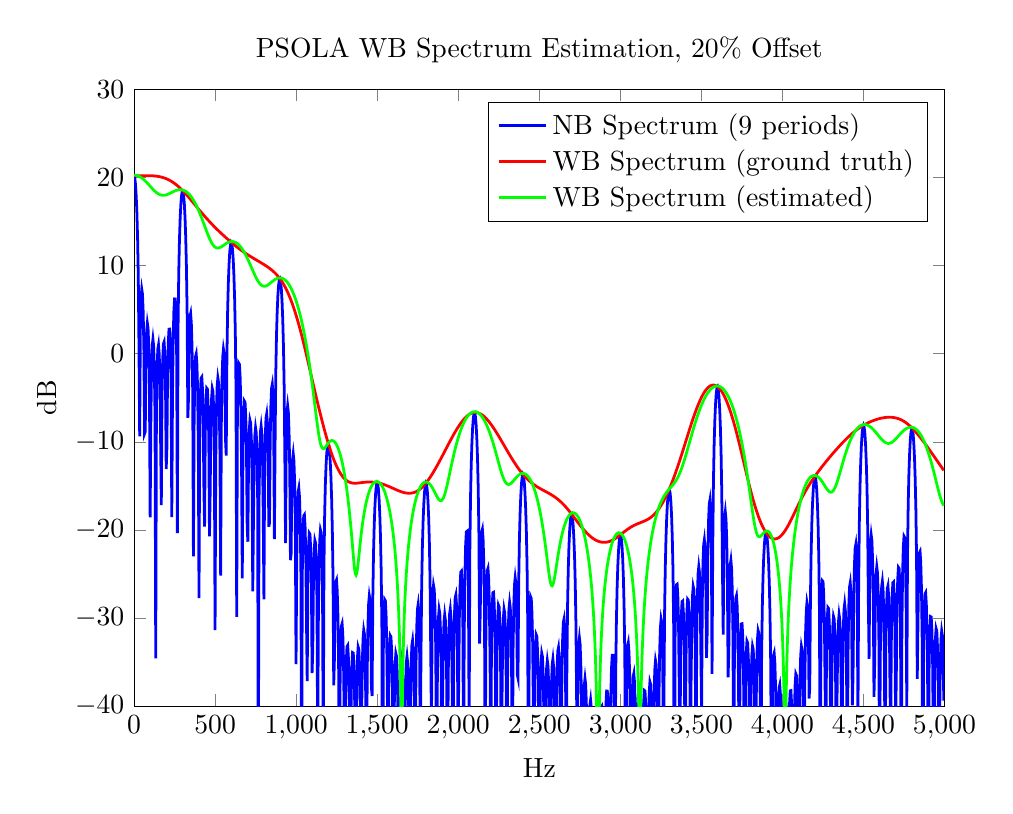
\begin{tikzpicture}

\begin{axis}[%
width=4.052in,
height=3.084in,
at={(0.68in,0.416in)},
scale only axis,
xmin=0,
xmax=5000,
xlabel={Hz},
ymin=-40,
ymax=30,
ylabel={dB},
axis background/.style={fill=white},
title={PSOLA WB Spectrum Estimation, 20\% Offset},
legend style={legend cell align=left,align=left,legend plot pos=left,draw=black}
]
\addplot [color=blue,solid,line width=1.0pt]
  table[row sep=crcr]{%
0	20.1998112835222\\
4.306640625	19.9630253688939\\
8.61328125	19.2360845575318\\
12.919921875	17.9633168361555\\
17.2265625	16.0268836225403\\
21.533203125	13.180537695682\\
25.83984375	8.82254699381025\\
30.146484375	0.700132969808097\\
34.453125	-9.38373028135972\\
38.759765625	2.98659328058475\\
43.06640625	6.33169751815378\\
47.373046875	7.30266913618077\\
51.6796875	6.77667164223539\\
55.986328125	4.80429815421497\\
60.29296875	0.750174864059773\\
64.599609375	-9.06739986575636\\
68.90625	-8.84633812663461\\
73.212890625	-0.448845833559547\\
77.51953125	2.5403005536744\\
81.826171875	3.47160202128536\\
86.1328125	2.92848316932768\\
90.439453125	0.823665076872224\\
94.74609375	-3.79589942490457\\
99.052734375	-18.5756773333599\\
103.359375	-7.93671108111667\\
107.666015625	-1.59488202972874\\
111.97265625	0.938574790851837\\
116.279296875	1.65231303930877\\
120.5859375	0.911077829630306\\
124.892578125	-1.52749587117764\\
129.19921875	-7.11592771881383\\
133.505859375	-34.5722812401772\\
137.8125	-6.61373585025094\\
142.119140625	-1.57112851524897\\
146.42578125	0.545998657477225\\
150.732421875	1.00846814542794\\
155.0390625	0.00753024427498389\\
159.345703125	-2.88396851268621\\
163.65234375	-9.97838634972832\\
167.958984375	-17.1927718041873\\
172.265625	-4.78035058609264\\
176.572265625	-0.638401029402439\\
180.87890625	1.12216069547664\\
185.185546875	1.33907375557166\\
189.4921875	0.0523509699633727\\
193.798828125	-3.40616894653224\\
198.10546875	-13.0783607136449\\
202.412109375	-10.8149063853367\\
206.71875	-2.21399351427716\\
211.025390625	1.2932326952125\\
215.33203125	2.78023534109459\\
219.638671875	2.79677833190986\\
223.9453125	1.23710570621143\\
228.251953125	-2.90986314652361\\
232.55859375	-18.5287229748842\\
236.865234375	-5.07437946200521\\
241.171875	1.68146492127122\\
245.478515625	4.82865651916769\\
249.78515625	6.2251383823794\\
254.091796875	6.21700298464575\\
258.3984375	4.54902151417185\\
262.705078125	-0.316094354876905\\
267.01171875	-20.3631341734267\\
271.318359375	3.0575325482516\\
275.625	9.27891427842231\\
279.931640625	12.9384014511283\\
284.23828125	15.3605744062789\\
288.544921875	16.9768834776396\\
292.8515625	17.9772307831562\\
297.158203125	18.4540713750781\\
301.46484375	18.4483724573271\\
305.771484375	17.9654551343891\\
310.078125	16.9768328564373\\
314.384765625	15.4096529514292\\
318.69140625	13.1137629249197\\
322.998046875	9.76421522356002\\
327.3046875	4.48366650833135\\
331.611328125	-7.28779593916486\\
335.91796875	-4.96268408957308\\
340.224609375	1.99861917064307\\
344.53125	4.24016109828537\\
348.837890625	4.56604715190631\\
353.14453125	3.47389454839626\\
357.451171875	0.821822316752798\\
361.7578125	-4.4793399264641\\
366.064453125	-22.9871894100464\\
370.37109375	-7.92767303445529\\
374.677734375	-2.4009077695411\\
378.984375	-0.342290696274627\\
383.291015625	-0.0312863801554487\\
387.59765625	-1.16210097745387\\
391.904296875	-4.03150884435551\\
396.2109375	-10.3064811168369\\
400.517578125	-27.7454720012042\\
404.82421875	-8.96041617777776\\
409.130859375	-4.50057833605844\\
413.4375	-2.76654864977965\\
417.744140625	-2.64331898403537\\
422.05078125	-3.98848799706377\\
426.357421875	-7.29656530604883\\
430.6640625	-15.2784849930523\\
434.970703125	-19.6280359003298\\
439.27734375	-8.99724258837361\\
443.583984375	-5.32514630847748\\
447.890625	-3.90870070723117\\
452.197265625	-4.01131670320744\\
456.50390625	-5.63872381985393\\
460.810546875	-9.55198582122405\\
465.1171875	-20.7180942624329\\
469.423828125	-15.7930568669292\\
473.73046875	-8.16917574371243\\
478.037109375	-5.08890608921028\\
482.34375	-3.95112449656558\\
486.650390625	-4.27886302677546\\
490.95703125	-6.22662574650125\\
495.263671875	-10.9467752816124\\
499.5703125	-31.3720854955781\\
503.876953125	-12.3005026495531\\
508.18359375	-6.31416655720202\\
512.490234375	-3.66153375393449\\
516.796875	-2.73342069721742\\
521.103515625	-3.24679935077833\\
525.41015625	-5.52163956819098\\
529.716796875	-11.3416106283318\\
534.0234375	-25.1884263224476\\
538.330078125	-7.88815132235102\\
542.63671875	-2.83702992295379\\
546.943359375	-0.390317992662059\\
551.25	0.506453767531607\\
555.556640625	-0.0166482969133403\\
559.86328125	-2.47547139389485\\
564.169921875	-9.79720344227454\\
568.4765625	-11.5585700714678\\
572.783203125	-0.260917670788041\\
577.08984375	4.80216728799505\\
581.396484375	7.96660497742971\\
585.703125	10.0888756045376\\
590.009765625	11.4884644993177\\
594.31640625	12.3134403650122\\
598.623046875	12.6356434402504\\
602.9296875	12.4829286915673\\
607.236328125	11.8494208999965\\
611.54296875	10.6934370617096\\
615.849609375	8.92126187582147\\
620.15625	6.34018611552969\\
624.462890625	2.51060127598473\\
628.76953125	-3.93058726765696\\
633.076171875	-29.8765921370504\\
637.3828125	-7.22073387554979\\
641.689453125	-2.58802074239123\\
645.99609375	-1.08406020592237\\
650.302734375	-1.22451821675793\\
654.609375	-2.76748144168745\\
658.916015625	-6.07369842266098\\
663.22265625	-13.0703615125042\\
667.529296875	-25.4888922745812\\
671.8359375	-10.7681475759189\\
676.142578125	-6.80085219175046\\
680.44921875	-5.37724854639443\\
684.755859375	-5.51878242265869\\
689.0625	-7.1315311122338\\
693.369140625	-10.7845917295229\\
697.67578125	-19.6906547805135\\
701.982421875	-21.331947444522\\
706.2890625	-12.0232587584064\\
710.595703125	-8.70507389456911\\
714.90234375	-7.52962795903941\\
719.208984375	-7.85076038400367\\
723.515625	-9.72012802481867\\
727.822265625	-14.0032074625755\\
732.12890625	-26.9681252466484\\
736.435546875	-18.9683572216046\\
740.7421875	-12.0946118990068\\
745.048828125	-9.31566283462937\\
749.35546875	-8.40778630849761\\
753.662109375	-8.96009418001901\\
757.96875	-11.1765633942772\\
762.275390625	-16.3715606156391\\
766.58203125	-50.4097779235462\\
770.888671875	-16.649390269191\\
775.1953125	-11.2182619719317\\
779.501953125	-8.87541873477621\\
783.80859375	-8.21734155257196\\
788.115234375	-9.01485145668904\\
792.421875	-11.6480762232233\\
796.728515625	-18.1820357938765\\
801.03515625	-27.8814763418916\\
805.341796875	-13.7899449945592\\
809.6484375	-9.29777925877496\\
813.955078125	-7.28269765023121\\
818.26171875	-6.82222429053385\\
822.568359375	-7.84092958267098\\
826.875	-10.9426873551596\\
831.181640625	-19.6363187515666\\
835.48828125	-19.2147076680975\\
839.794921875	-9.70840578203416\\
844.1015625	-5.77334921409505\\
848.408203125	-3.89682282661396\\
852.71484375	-3.46440523501345\\
857.021484375	-4.5384695767372\\
861.328125	-8.0257594005086\\
865.634765625	-21.0448365225365\\
869.94140625	-10.0975056717451\\
874.248046875	-2.195712077007\\
878.5546875	2.03661305204502\\
882.861328125	4.77327991030721\\
887.16796875	6.60322091770327\\
891.474609375	7.76851277988212\\
895.78125	8.38504242800249\\
900.087890625	8.50728188270865\\
904.39453125	8.15087262548289\\
908.701171875	7.2982955639766\\
913.0078125	5.89269374756126\\
917.314453125	3.81429303836856\\
921.62109375	0.812655230261074\\
925.927734375	-3.72703921020973\\
930.234375	-12.1406550808728\\
934.541015625	-21.4830175679408\\
938.84765625	-9.79456922700259\\
943.154296875	-6.68408706564325\\
947.4609375	-5.91921294684327\\
951.767578125	-6.65127897304316\\
956.07421875	-8.84128343273207\\
960.380859375	-13.1459599848905\\
964.6875	-23.4280461085132\\
968.994140625	-22.709719872331\\
973.30078125	-14.7526519311194\\
977.607421875	-12.0393831716497\\
981.9140625	-11.3674018549286\\
986.220703125	-12.1729621553081\\
990.52734375	-14.554974476215\\
994.833984375	-19.4978085436939\\
999.140625	-35.2394625173893\\
1003.447265625	-23.7992519007091\\
1007.75390625	-17.8583238819868\\
1012.060546875	-15.6433421617602\\
1016.3671875	-15.237997396714\\
1020.673828125	-16.2922529627976\\
1024.98046875	-19.0614079921665\\
1029.287109375	-25.0486132711531\\
1033.59375	-49.0489298744527\\
1037.900390625	-24.8089499761534\\
1042.20703125	-20.1642092960551\\
1046.513671875	-18.3960011512\\
1050.8203125	-18.2748293831415\\
1055.126953125	-19.6214733178922\\
1059.43359375	-22.8791188728092\\
1063.740234375	-30.4530193089661\\
1068.046875	-37.1668211819933\\
1072.353515625	-25.5193434711999\\
1076.66015625	-21.7657194537968\\
1080.966796875	-20.3597785467106\\
1085.2734375	-20.4901021210194\\
1089.580078125	-22.127753296442\\
1093.88671875	-25.9629911891354\\
1098.193359375	-36.246288353504\\
1102.5	-33.579043475189\\
1106.806640625	-25.4932347862979\\
1111.11328125	-22.3449523604847\\
1115.419921875	-21.1911146165028\\
1119.7265625	-21.5004356503055\\
1124.033203125	-23.3902174237449\\
1128.33984375	-27.9048897074595\\
1132.646484375	-44.7102230597605\\
1136.953125	-30.2833775016506\\
1141.259765625	-23.9262840157376\\
1145.56640625	-21.0912950068375\\
1149.873046875	-19.9863411636628\\
1154.1796875	-20.279564559475\\
1158.486328125	-22.2395319531199\\
1162.79296875	-27.4586537681424\\
1167.099609375	-45.5842743246826\\
1171.40625	-24.2089204093871\\
1175.712890625	-18.2949510731541\\
1180.01953125	-14.8851512980094\\
1184.326171875	-12.691793179793\\
1188.6328125	-11.2912626612358\\
1192.939453125	-10.4963177591208\\
1197.24609375	-10.2156703212552\\
1201.552734375	-10.4090021409064\\
1205.859375	-11.0714974932495\\
1210.166015625	-12.2322431141108\\
1214.47265625	-13.9650961185263\\
1218.779296875	-16.4223268513851\\
1223.0859375	-19.9344917157253\\
1227.392578125	-25.4005568635528\\
1231.69921875	-37.6231868881101\\
1236.005859375	-34.6680737629009\\
1240.3125	-27.994825560824\\
1244.619140625	-25.8959841344629\\
1248.92578125	-25.683528706939\\
1253.232421875	-26.8777749478328\\
1257.5390625	-29.6326456080537\\
1261.845703125	-35.0734362938085\\
1266.15234375	-54.8514097573601\\
1270.458984375	-38.2663073589712\\
1274.765625	-32.8892469234498\\
1279.072265625	-30.8979252819675\\
1283.37890625	-30.6323479254595\\
1287.685546875	-31.8008987748611\\
1291.9921875	-34.7145473825549\\
1296.298828125	-41.1009369688574\\
1300.60546875	-56.9684224491254\\
1304.912109375	-39.3767009237428\\
1309.21875	-34.9724360950563\\
1313.525390625	-33.2423355395328\\
1317.83203125	-33.1077098181897\\
1322.138671875	-34.4384930600509\\
1326.4453125	-37.7474979121764\\
1330.751953125	-45.8624166843514\\
1335.05859375	-49.4140706504964\\
1339.365234375	-39.0528066719654\\
1343.671875	-35.3738318088744\\
1347.978515625	-33.9175038023049\\
1352.28515625	-33.9714153074006\\
1356.591796875	-35.5531776289137\\
1360.8984375	-39.4494940305821\\
1365.205078125	-50.9154625398585\\
1369.51171875	-45.1326337947302\\
1373.818359375	-37.5949215377083\\
1378.125	-34.4764153065035\\
1382.431640625	-33.2801179057106\\
1386.73828125	-33.5465690198466\\
1391.044921875	-35.442810828673\\
1395.3515625	-40.1602796322515\\
1399.658203125	-62.3297224810393\\
1403.96484375	-40.9954863426594\\
1408.271484375	-35.0323309007632\\
1412.578125	-32.3354466062052\\
1416.884765625	-31.3511525962668\\
1421.19140625	-31.8101434649747\\
1425.498046875	-34.046959405141\\
1429.8046875	-39.9115330777737\\
1434.111328125	-52.4321846741827\\
1438.41796875	-35.9521220254251\\
1442.724609375	-30.9035515648031\\
1447.03125	-28.4187098024568\\
1451.337890625	-27.4766849716494\\
1455.64453125	-27.9592258329553\\
1459.951171875	-30.4009573586294\\
1464.2578125	-37.8600226117026\\
1468.564453125	-38.8379538202033\\
1472.87109375	-27.7690945672026\\
1477.177734375	-22.699252507885\\
1481.484375	-19.4999587165494\\
1485.791015625	-17.3350331009931\\
1490.09765625	-15.8904446411636\\
1494.404296875	-15.0202858544826\\
1498.7109375	-14.6538325756486\\
1503.017578125	-14.763980876241\\
1507.32421875	-15.3572926702582\\
1511.630859375	-16.4763102847611\\
1515.9375	-18.2161636858893\\
1520.244140625	-20.7725504988485\\
1524.55078125	-24.593560318074\\
1528.857421875	-31.0824962855242\\
1533.1640625	-60.4598649948022\\
1537.470703125	-33.9555491987503\\
1541.77734375	-29.3921165970853\\
1546.083984375	-27.8964933617719\\
1550.390625	-28.0350725088891\\
1554.697265625	-29.5790381622938\\
1559.00390625	-32.9040089035676\\
1563.310546875	-40.0097778309555\\
1567.6171875	-51.3457965177724\\
1571.923828125	-37.3078224679822\\
1576.23046875	-33.3955540299073\\
1580.537109375	-31.9889397035259\\
1584.84375	-32.1406957438218\\
1589.150390625	-33.7684943613522\\
1593.45703125	-37.461074618364\\
1597.763671875	-46.5793964602232\\
1602.0703125	-47.5026766593959\\
1606.376953125	-38.4446636874249\\
1610.68359375	-35.1711415105569\\
1614.990234375	-34.0147420882645\\
1619.296875	-34.3504665004912\\
1623.603515625	-36.2413845084006\\
1627.91015625	-40.5813332190181\\
1632.216796875	-54.0586877968533\\
1636.5234375	-45.1511662193199\\
1640.830078125	-38.4103418998207\\
1645.13671875	-35.6618951858327\\
1649.443359375	-34.765945852533\\
1653.75	-35.3272437045274\\
1658.056640625	-37.5623193933281\\
1662.36328125	-42.8305154979651\\
1666.669921875	-104.975649309368\\
1670.9765625	-42.7176261684347\\
1675.283203125	-37.3554006713557\\
1679.58984375	-35.0202604587396\\
1683.896484375	-34.3553669793566\\
1688.203125	-35.1442114329868\\
1692.509765625	-37.7822420781882\\
1696.81640625	-44.4144001495545\\
1701.123046875	-53.1280943956726\\
1705.4296875	-39.557383620042\\
1709.736328125	-35.0795141923781\\
1714.04296875	-33.0373838420722\\
1718.349609375	-32.537675104167\\
1722.65625	-33.5163269255627\\
1726.962890625	-36.5977631423763\\
1731.26953125	-45.4597924187348\\
1735.576171875	-44.2477100992935\\
1739.8828125	-34.8845159778428\\
1744.189453125	-30.9041931763623\\
1748.49609375	-28.9515049463273\\
1752.802734375	-28.4320019136335\\
1757.109375	-29.4194416822271\\
1761.416015625	-32.8506957161765\\
1765.72265625	-46.3693479059954\\
1770.029296875	-34.2808557895966\\
1774.3359375	-26.3628142786716\\
1778.642578125	-22.012212267465\\
1782.94921875	-19.1298878090504\\
1787.255859375	-17.1389723439664\\
1791.5625	-15.8011055204505\\
1795.869140625	-15.0019564760371\\
1800.17578125	-14.6878788442319\\
1804.482421875	-14.8438126989631\\
1808.7890625	-15.4878698935034\\
1813.095703125	-16.6777739056355\\
1817.40234375	-18.5349570979253\\
1821.708984375	-21.3138581276861\\
1826.015625	-25.6425256313867\\
1830.322265625	-33.9442357631557\\
1834.62890625	-42.1597878516606\\
1838.935546875	-30.6691442082378\\
1843.2421875	-27.3358130752316\\
1847.548828125	-26.3048331016152\\
1851.85546875	-26.7550654832247\\
1856.162109375	-28.6590153040817\\
1860.46875	-32.6953363038248\\
1864.775390625	-42.9213312966232\\
1869.08203125	-41.1489301883569\\
1873.388671875	-33.0534286338037\\
1877.6953125	-30.0312904603135\\
1882.001953125	-29.0189732567229\\
1886.30859375	-29.4721500512705\\
1890.615234375	-31.5017047311995\\
1894.921875	-36.1247461605529\\
1899.228515625	-52.2578341102143\\
1903.53515625	-39.257415060976\\
1907.841796875	-33.0260082349903\\
1912.1484375	-30.4289480557643\\
1916.455078125	-29.6194221961028\\
1920.76171875	-30.262464662772\\
1925.068359375	-32.6271824401265\\
1929.375	-38.2703220889431\\
1933.681640625	-59.1053156735768\\
1937.98828125	-36.7723546280088\\
1942.294921875	-31.7508918386798\\
1946.6015625	-29.5519867758319\\
1950.908203125	-28.9868558169204\\
1955.21484375	-29.8891711266675\\
1959.521484375	-32.7195201566249\\
1963.828125	-39.9823078447383\\
1968.134765625	-45.4239550221179\\
1972.44140625	-33.7083735260088\\
1976.748046875	-29.5421199220567\\
1981.0546875	-27.6922591596885\\
1985.361328125	-27.373922383357\\
1989.66796875	-28.5702431157747\\
1993.974609375	-31.9952016286193\\
1998.28125	-42.1255368344246\\
2002.587890625	-38.2680387530637\\
2006.89453125	-29.9185333260343\\
2011.201171875	-26.3667689335384\\
2015.5078125	-24.7931589442721\\
2019.814453125	-24.6852642225431\\
2024.12109375	-26.1727921058266\\
2028.427734375	-30.3354640337953\\
2032.734375	-47.7581845535017\\
2037.041015625	-31.523196112068\\
2041.34765625	-24.876446907335\\
2045.654296875	-21.6822384967924\\
2049.9609375	-20.2118969681157\\
2054.267578125	-20.1480821852721\\
2058.57421875	-21.7734467574225\\
2062.880859375	-26.7385880562228\\
2067.1875	-42.708700428162\\
2071.494140625	-22.4378312304649\\
2075.80078125	-16.268347544036\\
2080.107421875	-12.5651348389637\\
2084.4140625	-10.0764442180625\\
2088.720703125	-8.38683419825366\\
2093.02734375	-7.31216979394629\\
2097.333984375	-6.7627752268266\\
2101.640625	-6.69940453707979\\
2105.947265625	-7.11814163178113\\
2110.25390625	-8.04903307402283\\
2114.560546875	-9.56726083744622\\
2118.8671875	-11.8275001917677\\
2123.173828125	-15.1662322951206\\
2127.48046875	-20.5049129293377\\
2131.787109375	-32.9100769045871\\
2136.09375	-29.0395782303147\\
2140.400390625	-22.3989845730526\\
2144.70703125	-20.216793504205\\
2149.013671875	-19.9144194854456\\
2153.3203125	-21.0295818274495\\
2157.626953125	-23.7281883666489\\
2161.93359375	-29.1728089073116\\
2166.240234375	-50.3589227083544\\
2170.546875	-31.9000210182524\\
2174.853515625	-26.5942818768441\\
2179.16015625	-24.6152615654851\\
2183.466796875	-24.3604339158489\\
2187.7734375	-25.5516873228188\\
2192.080078125	-28.5139349482537\\
2196.38671875	-35.0378142404274\\
2200.693359375	-49.554029092935\\
2205	-33.0309637153544\\
2209.306640625	-28.7545838765739\\
2213.61328125	-27.1184416954249\\
2217.919921875	-27.0782027772328\\
2222.2265625	-28.5153083048277\\
2226.533203125	-31.9605190444566\\
2230.83984375	-40.3646109213481\\
2235.146484375	-43.2906400808699\\
2239.453125	-33.3493502412746\\
2243.759765625	-29.8439687825046\\
2248.06640625	-28.5387648225808\\
2252.373046875	-28.7439277105515\\
2256.6796875	-30.4880394813397\\
2260.986328125	-34.5832900040212\\
2265.29296875	-46.5990097123003\\
2269.599609375	-40.1606439750171\\
2273.90625	-32.9316172930479\\
2278.212890625	-30.0067637592205\\
2282.51953125	-28.9867621626858\\
2286.826171875	-29.4284880457928\\
2291.1328125	-31.5108852154617\\
2295.439453125	-36.4652544837721\\
2299.74609375	-61.2066593100598\\
2304.052734375	-37.2553728178305\\
2308.359375	-31.5458712771851\\
2312.666015625	-29.035643615261\\
2316.97265625	-28.2236888746236\\
2321.279296875	-28.8538076898643\\
2325.5859375	-31.2750064812107\\
2329.892578125	-37.4064015955918\\
2334.19921875	-48.9209090606158\\
2338.505859375	-33.3616871250172\\
2342.8125	-28.5190609187449\\
2347.119140625	-26.1964438496571\\
2351.42578125	-25.405220410786\\
2355.732421875	-26.0387521508391\\
2360.0390625	-28.6507573839285\\
2364.345703125	-36.4386239401824\\
2368.65234375	-36.8163491943689\\
2372.958984375	-26.1301111832324\\
2377.265625	-21.2175341126822\\
2381.572265625	-18.142535171817\\
2385.87890625	-16.0884878695765\\
2390.185546875	-14.7466392148609\\
2394.4921875	-13.9731773329578\\
2398.798828125	-13.6984663538312\\
2403.10546875	-13.8961398044653\\
2407.412109375	-14.5734375108637\\
2411.71875	-15.7737572192914\\
2416.025390625	-17.5936551150677\\
2420.33203125	-20.2318764371414\\
2424.638671875	-24.1452343518514\\
2428.9453125	-30.7789852175617\\
2433.251953125	-66.4019714005567\\
2437.55859375	-33.4074736682387\\
2441.865234375	-28.987962257558\\
2446.171875	-27.5724058903906\\
2450.478515625	-27.7760166309201\\
2454.78515625	-29.3830933938643\\
2459.091796875	-32.7846132055057\\
2463.3984375	-40.0568646178564\\
2467.705078125	-50.4272465723129\\
2472.01171875	-37.0441163688065\\
2476.318359375	-33.2257025076207\\
2480.625	-31.8728563210116\\
2484.931640625	-32.0688774796672\\
2489.23828125	-33.7433360633389\\
2493.544921875	-37.5054889999806\\
2497.8515625	-46.8750563107116\\
2502.158203125	-47.1081249117755\\
2506.46484375	-38.3111303772849\\
2510.771484375	-35.1047564400771\\
2515.078125	-33.9902587211159\\
2519.384765625	-34.3636517375759\\
2523.69140625	-36.2998882110528\\
2527.998046875	-40.7225502599253\\
2532.3046875	-54.7896259723685\\
2536.611328125	-44.9542860085908\\
2540.91796875	-38.3705088203463\\
2545.224609375	-35.6840327972781\\
2549.53125	-34.8350881342123\\
2553.837890625	-35.4442094639198\\
2558.14453125	-37.7410973198588\\
2562.451171875	-43.1324081573405\\
2566.7578125	-76.1903742019872\\
2571.064453125	-42.7385826262528\\
2575.37109375	-37.5061328476314\\
2579.677734375	-35.2482304782899\\
2583.984375	-34.6533440754984\\
2588.291015625	-35.5179554296034\\
2592.59765625	-38.2536050675571\\
2596.904296875	-45.0898161596529\\
2601.2109375	-52.9737074838001\\
2605.517578125	-39.9911606084764\\
2609.82421875	-35.6541297611105\\
2614.130859375	-33.7228341105146\\
2618.4375	-33.3326144968328\\
2622.744140625	-34.431166579502\\
2627.05078125	-37.6644405259101\\
2631.357421875	-46.891886904165\\
2635.6640625	-45.0820004386549\\
2639.970703125	-36.0577487702048\\
2644.27734375	-32.2516534925379\\
2648.583984375	-30.456208457312\\
2652.890625	-30.0967095589726\\
2657.197265625	-31.2586116410841\\
2661.50390625	-34.9101754842159\\
2665.810546875	-49.2903420505588\\
2670.1171875	-36.2939839737482\\
2674.423828125	-28.6721665421373\\
2678.73046875	-24.5341727714305\\
2683.037109375	-21.8517686865512\\
2687.34375	-20.0597004739853\\
2691.650390625	-18.9230923415622\\
2695.95703125	-18.3289537736819\\
2700.263671875	-18.2242397382096\\
2704.5703125	-18.5942402492394\\
2708.876953125	-19.4574264964143\\
2713.18359375	-20.8721590766889\\
2717.490234375	-22.9613131717362\\
2721.796875	-25.9831650620963\\
2726.103515625	-30.5791306822711\\
2730.41015625	-39.2645015623732\\
2734.716796875	-46.8868912081727\\
2739.0234375	-36.0683906140521\\
2743.330078125	-33.0340079398172\\
2747.63671875	-32.2705155956855\\
2751.943359375	-32.983141617458\\
2756.25	-35.1555622573567\\
2760.556640625	-39.4886561707437\\
2764.86328125	-50.2490157418892\\
2769.169921875	-47.9977935954882\\
2773.4765625	-40.3451102434544\\
2777.783203125	-37.6128311072676\\
2782.08984375	-36.8675804163977\\
2786.396484375	-37.5835646475393\\
2790.703125	-39.8832746168773\\
2795.009765625	-44.8172531012501\\
2799.31640625	-62.0877268366828\\
2803.623046875	-48.0597883289766\\
2807.9296875	-42.1796095214999\\
2812.236328125	-39.850498316468\\
2816.54296875	-39.2913922967276\\
2820.849609375	-40.181558693505\\
2825.15625	-42.8034887160782\\
2829.462890625	-48.7692269644519\\
2833.76953125	-67.6710190603224\\
2838.076171875	-47.3425535143462\\
2842.3828125	-42.6081152478516\\
2846.689453125	-40.6435224122418\\
2850.99609375	-40.2984757190075\\
2855.302734375	-41.4186741297192\\
2859.609375	-44.4817140564073\\
2863.916015625	-52.0960084439547\\
2868.22265625	-56.939576564549\\
2872.529296875	-45.7727514113484\\
2876.8359375	-41.8325635694862\\
2881.142578125	-40.1717222817265\\
2885.44921875	-40.0303520492362\\
2889.755859375	-41.402890184059\\
2894.0625	-45.0269874700971\\
2898.369140625	-55.6237059565789\\
2902.67578125	-51.1512579611434\\
2906.982421875	-43.106376082989\\
2911.2890625	-39.7154560459105\\
2915.595703125	-38.2746719849119\\
2919.90234375	-38.2893844680599\\
2924.208984375	-39.9011946186281\\
2928.515625	-44.2258187205749\\
2932.822265625	-62.9494539894544\\
2937.12890625	-45.20416419073\\
2941.435546875	-38.7302720219932\\
2945.7421875	-35.6264854791727\\
2950.048828125	-34.2243062951739\\
2954.35546875	-34.220291840784\\
2958.662109375	-35.9110167472255\\
2962.96875	-41.0075527373224\\
2967.275390625	-55.4321085229669\\
2971.58203125	-36.3630249381074\\
2975.888671875	-30.2626760136278\\
2980.1953125	-26.5734731289619\\
2984.501953125	-24.078095669258\\
2988.80859375	-22.3689574290012\\
2993.115234375	-21.2649081185316\\
2997.421875	-20.6778419447195\\
3001.728515625	-20.5695944891797\\
3006.03515625	-20.9371997656282\\
3010.341796875	-21.8117530474599\\
3014.6484375	-23.2698926232029\\
3018.955078125	-25.4688899689393\\
3023.26171875	-28.7514749790093\\
3027.568359375	-34.0626002178549\\
3031.875	-46.7567933837926\\
3036.181640625	-42.0140647141125\\
3040.48828125	-35.4435329180323\\
3044.794921875	-33.2047814029782\\
3049.1015625	-32.8229357294588\\
3053.408203125	-33.853055362479\\
3057.71484375	-36.4734686098061\\
3062.021484375	-41.885772554196\\
3066.328125	-64.8001384985309\\
3070.634765625	-44.0256507891853\\
3074.94140625	-38.7036744803229\\
3079.248046875	-36.6377587337947\\
3083.5546875	-36.2807343098695\\
3087.861328125	-37.3681605304621\\
3092.16796875	-40.2395008626668\\
3096.474609375	-46.75175834256\\
3100.78125	-59.8863713418095\\
3105.087890625	-44.1156968253799\\
3109.39453125	-39.7750411909474\\
3113.701171875	-38.0305600785413\\
3118.0078125	-37.8714321790394\\
3122.314453125	-39.1908994264135\\
3126.62109375	-42.5385019620826\\
3130.927734375	-50.996269243384\\
3135.234375	-53.0517320032755\\
3139.541015625	-43.2478666730607\\
3143.84765625	-39.6420742745509\\
3148.154296875	-38.2063564403349\\
3152.4609375	-38.27326957514\\
3156.767578125	-39.8828059491262\\
3161.07421875	-43.8738874749665\\
3165.380859375	-56.1615792805698\\
3169.6875	-48.7221387693273\\
3173.994140625	-41.4716201956768\\
3178.30078125	-38.4104877986395\\
3182.607421875	-37.232334849377\\
3186.9140625	-37.5104322603686\\
3191.220703125	-39.4361475502621\\
3195.52734375	-44.2826065316391\\
3199.833984375	-72.3506328331899\\
3204.140625	-44.3239033174075\\
3208.447265625	-38.508211668137\\
3212.75390625	-35.8248824814399\\
3217.060546875	-34.8237049563143\\
3221.3671875	-35.261700656896\\
3225.673828125	-37.5028864137859\\
3229.98046875	-43.5392487927682\\
3234.287109375	-53.7643667312617\\
3238.59375	-38.6700987201614\\
3242.900390625	-33.6625174686423\\
3247.20703125	-31.1321120878291\\
3251.513671875	-30.1216839461902\\
3255.8203125	-30.5363663846188\\
3260.126953125	-32.949699653548\\
3264.43359375	-40.7078270498552\\
3268.740234375	-40.1211212656282\\
3273.046875	-29.4343011190198\\
3277.353515625	-24.3111897390541\\
3281.66015625	-20.9948615767834\\
3285.966796875	-18.6877990173082\\
3290.2734375	-17.0865656035023\\
3294.580078125	-16.0495393873017\\
3298.88671875	-15.5082678115976\\
3303.193359375	-15.437209479094\\
3307.5	-15.8443631517951\\
3311.806640625	-16.7740590742392\\
3316.11328125	-18.3243586101523\\
3320.419921875	-20.6971585827839\\
3324.7265625	-24.3582545035936\\
3329.033203125	-30.7966632455941\\
3333.33984375	-87.898308503967\\
3337.646484375	-32.5023850324611\\
3341.953125	-27.8882052865314\\
3346.259765625	-26.2187432694613\\
3350.56640625	-26.1560297487135\\
3354.873046875	-27.4972729398102\\
3359.1796875	-30.6490528995852\\
3363.486328125	-37.7680234425667\\
3367.79296875	-46.9060882406758\\
3372.099609375	-33.7968149279235\\
3376.40625	-29.7516183777346\\
3380.712890625	-28.1349599333455\\
3385.01953125	-28.0596503708899\\
3389.326171875	-29.467031045515\\
3393.6328125	-32.9873491078435\\
3397.939453125	-42.3101800080251\\
3402.24609375	-41.5434651589063\\
3406.552734375	-32.6866965230436\\
3410.859375	-29.2399168429454\\
3415.166015625	-27.8619762418519\\
3419.47265625	-27.969367348393\\
3423.779296875	-29.6489764186699\\
3428.0859375	-33.8551250672344\\
3432.392578125	-48.2737978570864\\
3436.69921875	-37.155285439225\\
3441.005859375	-30.4269835467674\\
3445.3125	-27.5067787922715\\
3449.619140625	-26.4111293040105\\
3453.92578125	-26.7760731970912\\
3458.232421875	-28.8446485372534\\
3462.5390625	-34.0727954023431\\
3466.845703125	-60.8312370801053\\
3471.15234375	-32.8238852301067\\
3475.458984375	-27.433849934354\\
3479.765625	-24.9693002744062\\
3484.072265625	-24.1622093019711\\
3488.37890625	-24.8218552108221\\
3492.685546875	-27.3761422467702\\
3496.9921875	-34.1436421553486\\
3501.298828125	-40.9591739816712\\
3505.60546875	-28.2447451098672\\
3509.912109375	-23.7716761263398\\
3514.21875	-21.6764462723872\\
3518.525390625	-21.1221008386829\\
3522.83203125	-22.0680036202678\\
3527.138671875	-25.1821726879801\\
3531.4453125	-34.5192444999425\\
3535.751953125	-31.8361391692179\\
3540.05859375	-22.8701351695767\\
3544.365234375	-18.9681762457944\\
3548.671875	-17.0613476497315\\
3552.978515625	-16.5942517106421\\
3557.28515625	-17.6641790056877\\
3561.591796875	-21.271977885647\\
3565.8984375	-36.3384391390482\\
3570.205078125	-22.0843768220444\\
3574.51171875	-14.4923292148138\\
3578.818359375	-10.3061560656329\\
3583.125	-7.56547146462717\\
3587.431640625	-5.71671307315549\\
3591.73828125	-4.5288711563796\\
3596.044921875	-3.89076794039449\\
3600.3515625	-3.75047469524362\\
3604.658203125	-4.09416604142618\\
3608.96484375	-4.94121195811794\\
3613.271484375	-6.35114635341578\\
3617.578125	-8.44882395653159\\
3621.884765625	-11.496936074289\\
3626.19140625	-16.1511483228959\\
3630.498046875	-25.0244772708826\\
3634.8046875	-31.8867059962897\\
3639.111328125	-21.5214674090735\\
3643.41796875	-18.6076776165396\\
3647.724609375	-17.9436675380155\\
3652.03125	-18.7606058249232\\
3656.337890625	-21.0536835829067\\
3660.64453125	-25.5469853120076\\
3664.951171875	-36.7334938812177\\
3669.2578125	-33.8773788511342\\
3673.564453125	-26.5533109935897\\
3677.87109375	-24.0164773362994\\
3682.177734375	-23.4561643115808\\
3686.484375	-24.364838191111\\
3690.791015625	-26.8768173515131\\
3695.09765625	-32.0773934090619\\
3699.404296875	-50.5931716189613\\
3703.7109375	-35.375970378973\\
3708.017578125	-29.8329634357418\\
3712.32421875	-27.7731639324115\\
3716.630859375	-27.4781512387855\\
3720.9375	-28.641033146353\\
3725.244140625	-31.5577057211767\\
3729.55078125	-37.8977975230265\\
3733.857421875	-55.2812532811887\\
3738.1640625	-36.6704044693151\\
3742.470703125	-32.3014494149929\\
3746.77734375	-30.6615062142649\\
3751.083984375	-30.6369844289146\\
3755.390625	-32.0851180008102\\
3759.697265625	-35.5005042273147\\
3764.00390625	-43.6012611473214\\
3768.310546875	-48.0012627869981\\
3772.6171875	-37.5008205229226\\
3776.923828125	-33.9362508635276\\
3781.23046875	-32.6220178233208\\
3785.537109375	-32.822130126578\\
3789.84375	-34.5419603726996\\
3794.150390625	-38.5431782861696\\
3798.45703125	-49.8119539462272\\
3802.763671875	-44.8962245483157\\
3807.0703125	-37.3404272582706\\
3811.376953125	-34.3065508952583\\
3815.68359375	-33.1996908850795\\
3819.990234375	-33.5423154561426\\
3824.296875	-35.4877507046427\\
3828.603515625	-40.1888042178531\\
3832.91015625	-60.6868533208456\\
3837.216796875	-41.39379337141\\
3841.5234375	-35.3105491477842\\
3845.830078125	-32.5206145148892\\
3850.13671875	-31.4128202790261\\
3854.443359375	-31.6971938643931\\
3858.75	-33.6842398486729\\
3863.056640625	-39.1480971376655\\
3867.36328125	-52.4386834415479\\
3871.669921875	-34.6258237517792\\
3875.9765625	-28.8280826027843\\
3880.283203125	-25.3883670018722\\
3884.58984375	-23.1220693136767\\
3888.896484375	-21.6288175154311\\
3893.203125	-20.7299072326356\\
3897.509765625	-20.33826943484\\
3901.81640625	-20.4162825087401\\
3906.123046875	-20.9613913740309\\
3910.4296875	-22.0052094866458\\
3914.736328125	-23.625321246784\\
3919.04296875	-25.9811257412618\\
3923.349609375	-29.4212517010787\\
3927.65625	-34.9144985488446\\
3931.962890625	-48.1301517939177\\
3936.26953125	-42.688807619025\\
3940.576171875	-36.3720288025237\\
3944.8828125	-34.2599165531544\\
3949.189453125	-33.9753835547092\\
3953.49609375	-35.0901615566207\\
3957.802734375	-37.7948626624207\\
3962.109375	-43.3314065871638\\
3966.416015625	-68.7233902463632\\
3970.72265625	-45.1698694300168\\
3975.029296875	-39.9587219586994\\
3979.3359375	-37.9276930197624\\
3983.642578125	-37.5827082075015\\
3987.94921875	-38.6729362954293\\
3992.255859375	-41.5528365952521\\
3996.5625	-48.1492493356854\\
4000.869140625	-60.0919194311006\\
4005.17578125	-45.0433671452409\\
4009.482421875	-40.7081805705343\\
4013.7890625	-38.9208743767447\\
4018.095703125	-38.7035787727377\\
4022.40234375	-39.9619045651966\\
4026.708984375	-43.265330991318\\
4031.015625	-51.8363666589229\\
4035.322265625	-53.0754786121504\\
4039.62890625	-43.4379821518067\\
4043.935546875	-39.7758260182943\\
4048.2421875	-38.2547323736207\\
4052.548828125	-38.229874431845\\
4056.85546875	-39.7535475691503\\
4061.162109375	-43.6931223978237\\
4065.46875	-56.3461892477851\\
4069.775390625	-47.9316970843081\\
4074.08203125	-40.7181773106783\\
4078.388671875	-37.5905987623993\\
4082.6953125	-36.3313455051121\\
4087.001953125	-36.5303896757073\\
4091.30859375	-38.3922550156488\\
4095.615234375	-43.234116820216\\
4099.921875	-77.5919049398064\\
4104.228515625	-42.7561984344048\\
4108.53515625	-36.9604380747273\\
4112.841796875	-34.2427988599219\\
4117.1484375	-33.2020882258062\\
4121.455078125	-33.608620692722\\
4125.76171875	-35.841885627184\\
4130.068359375	-41.9705325509056\\
4134.375	-51.1679810891721\\
4138.681640625	-36.6717705453747\\
4142.98828125	-31.7133860218942\\
4147.294921875	-29.2016676846111\\
4151.6015625	-28.2096704400306\\
4155.908203125	-28.6540830580974\\
4160.21484375	-31.1285943315905\\
4164.521484375	-39.1380556874425\\
4168.828125	-37.8683400911948\\
4173.134765625	-27.4560839575006\\
4177.44140625	-22.4200931090986\\
4181.748046875	-19.1702080430285\\
4186.0546875	-16.9271646060258\\
4190.361328125	-15.3924780794908\\
4194.66796875	-14.4264335794054\\
4198.974609375	-13.9615033212945\\
4203.28125	-13.9727234892349\\
4207.587890625	-14.468611492929\\
4211.89453125	-15.4941969487991\\
4216.201171875	-17.1488258695487\\
4220.5078125	-19.6373635981454\\
4224.814453125	-23.4345787463369\\
4229.12109375	-30.0748967364654\\
4233.427734375	-63.8869409046795\\
4237.734375	-31.6658373912448\\
4242.041015625	-27.2672532852973\\
4246.34765625	-25.7619814440799\\
4250.654296875	-25.8567379433016\\
4254.9609375	-27.3611944387761\\
4259.267578125	-30.6975351525389\\
4263.57421875	-38.1066714040916\\
4267.880859375	-46.5009199140183\\
4272.1875	-34.0605247164625\\
4276.494140625	-30.236126113298\\
4280.80078125	-28.8073943374312\\
4285.107421875	-28.9152914713248\\
4289.4140625	-30.5124442775841\\
4293.720703125	-34.2501833507845\\
4298.02734375	-43.9997482977447\\
4302.333984375	-42.690641876449\\
4306.640625	-34.22229218336\\
4310.947265625	-30.9935243077054\\
4315.25390625	-29.8101622636356\\
4319.560546875	-30.1080469517845\\
4323.8671875	-31.9854189248997\\
4328.173828125	-36.4277324462624\\
4332.48046875	-51.7189862525618\\
4336.787109375	-39.6899809716274\\
4341.09375	-33.2502279576903\\
4345.400390625	-30.5277746861758\\
4349.70703125	-29.6110081010706\\
4354.013671875	-30.1505371225332\\
4358.3203125	-32.4022695523056\\
4362.626953125	-37.8728994289332\\
4366.93359375	-61.1166975838226\\
4371.240234375	-36.5463173265365\\
4375.546875	-31.3704599399011\\
4379.853515625	-29.0624621170011\\
4384.16015625	-28.395643370531\\
4388.466796875	-29.1914705790121\\
4392.7734375	-31.8941022845486\\
4397.080078125	-38.9156002828711\\
4401.38671875	-44.9989500525137\\
4405.693359375	-32.8054537546707\\
4410	-28.4719021960101\\
4414.306640625	-26.47554417908\\
4418.61328125	-26.0059731466628\\
4422.919921875	-27.0339147508144\\
4427.2265625	-30.2498147208535\\
4431.533203125	-39.9183607819267\\
4435.83984375	-36.5442599049321\\
4440.146484375	-27.8007302920081\\
4444.453125	-23.9606431446941\\
4448.759765625	-22.085116016838\\
4453.06640625	-21.6374220658491\\
4457.373046875	-22.7265986475699\\
4461.6796875	-26.3870787144713\\
4465.986328125	-42.329887259366\\
4470.29296875	-26.7707156984816\\
4474.599609375	-19.2491342754301\\
4478.90625	-15.0422376130894\\
4483.212890625	-12.2541052225542\\
4487.51953125	-10.3423630730968\\
4491.826171875	-9.0795963835618\\
4496.1328125	-8.3562082189104\\
4500.439453125	-8.12116370252309\\
4504.74609375	-8.36130623536975\\
4509.052734375	-9.09669968333317\\
4513.359375	-10.3878650166745\\
4517.666015625	-12.3614834127136\\
4521.97265625	-15.2845874829959\\
4526.279296875	-19.8273743727231\\
4530.5859375	-28.7061328945881\\
4534.892578125	-34.6221451122058\\
4539.19921875	-24.4531053219265\\
4543.505859375	-21.4112056885833\\
4547.8125	-20.5796366412841\\
4552.119140625	-21.2147220098272\\
4556.42578125	-23.3231775867827\\
4560.732421875	-27.6530273186601\\
4565.0390625	-38.9425767382805\\
4569.345703125	-35.1055753121824\\
4573.65234375	-27.7194705260882\\
4577.958984375	-24.9764684901373\\
4582.265625	-24.181707492025\\
4586.572265625	-24.8458050590187\\
4590.87890625	-27.1153680782757\\
4595.185546875	-32.1121467137223\\
4599.4921875	-51.5724026569041\\
4603.798828125	-34.4742002066132\\
4608.10546875	-28.7434755412787\\
4612.412109375	-26.416422324197\\
4616.71875	-25.8352306375824\\
4621.025390625	-26.7074622824445\\
4625.33203125	-29.3435415433163\\
4629.638671875	-35.4743121890495\\
4633.9453125	-50.9847890287294\\
4638.251953125	-33.2396079963893\\
4642.55859375	-28.6188562031977\\
4646.865234375	-26.6809560102724\\
4651.171875	-26.3489190036625\\
4655.478515625	-27.4926792475698\\
4659.78515625	-30.6255289173982\\
4664.091796875	-38.5832021111196\\
4668.3984375	-41.916795552149\\
4672.705078125	-31.4222113226116\\
4677.01171875	-27.596404018637\\
4681.318359375	-25.9960749874784\\
4685.625	-25.909628421414\\
4689.931640625	-27.3545599046565\\
4694.23828125	-31.1184507772551\\
4698.544921875	-42.477652793943\\
4702.8515625	-36.5002305023374\\
4707.158203125	-28.8370555881157\\
4711.46484375	-25.581331659219\\
4715.771484375	-24.2419866429776\\
4720.078125	-24.3590980174324\\
4724.384765625	-26.098659530333\\
4728.69140625	-30.6527694731462\\
4732.998046875	-52.794777485411\\
4737.3046875	-31.0806997464138\\
4741.611328125	-24.9062961654376\\
4745.91796875	-21.9681674588141\\
4750.224609375	-20.7104687918871\\
4754.53125	-20.8569153064109\\
4758.837890625	-22.7325590355733\\
4763.14453125	-28.177962723032\\
4767.451171875	-40.0977418381313\\
4771.7578125	-23.0524089142858\\
4776.064453125	-17.222693271396\\
4780.37109375	-13.7189446356193\\
4784.677734375	-11.3882639539286\\
4788.984375	-9.83753407324894\\
4793.291015625	-8.89065921707931\\
4797.59765625	-8.46178967574663\\
4801.904296875	-8.51402639424609\\
4806.2109375	-9.0453937397562\\
4810.517578125	-10.0881767940732\\
4814.82421875	-11.7210454262671\\
4819.130859375	-14.105666221705\\
4823.4375	-17.5967838293379\\
4827.744140625	-23.1879510020181\\
4832.05078125	-36.8944864593681\\
4836.357421875	-30.6835479592727\\
4840.6640625	-24.5923760514413\\
4844.970703125	-22.6057979022391\\
4849.27734375	-22.4392941121155\\
4853.583984375	-23.6808422413688\\
4857.890625	-26.533355954609\\
4862.197265625	-32.2805130334332\\
4866.50390625	-61.3911772198352\\
4870.810546875	-34.0483647868455\\
4875.1171875	-29.0903536544077\\
4879.423828125	-27.2589678595479\\
4883.73046875	-27.110635491222\\
4888.037109375	-28.4075051551957\\
4892.34375	-31.5187941372004\\
4896.650390625	-38.4440523030812\\
4900.95703125	-49.5358244093283\\
4905.263671875	-35.3966788182246\\
4909.5703125	-31.3551008544895\\
4913.876953125	-29.8294767479422\\
4918.18359375	-29.8728799714812\\
4922.490234375	-31.4022401996396\\
4926.796875	-35.0064212594587\\
4931.103515625	-44.0566037331007\\
4935.41015625	-44.8485436957538\\
4939.716796875	-35.7354362738379\\
4944.0234375	-32.3965138666402\\
4948.330078125	-31.1766006455004\\
4952.63671875	-31.4516423281939\\
4956.943359375	-33.2850109850823\\
4961.25	-37.5721775922188\\
4965.556640625	-51.0340132873053\\
4969.86328125	-42.0032084716122\\
4974.169921875	-35.2184504886396\\
4978.4765625	-32.4189162313148\\
4982.783203125	-31.4702887522931\\
4987.08984375	-31.9779635562361\\
4991.396484375	-34.1588730064248\\
4995.703125	-39.3751820424122\\
};
\addlegendentry{NB Spectrum (9 periods)};

\addplot [color=red,solid,line width=1.0pt]
  table[row sep=crcr]{%
0	20.1998112835222\\
4.306640625	20.1999011742825\\
8.61328125	20.2001691995733\\
12.919921875	20.2006103105267\\
17.2265625	20.2012157743361\\
21.533203125	20.201972828705\\
25.83984375	20.2028644145719\\
30.146484375	20.2038691110386\\
34.453125	20.2049613351258\\
38.759765625	20.2061117844833\\
43.06640625	20.2072880219475\\
47.373046875	20.2084550540905\\
51.6796875	20.2095757585421\\
55.986328125	20.2106110676231\\
60.29296875	20.2115199026489\\
64.599609375	20.2122589461967\\
68.90625	20.2127824076396\\
73.212890625	20.2130419562457\\
77.51953125	20.2129869569652\\
81.826171875	20.2125650558917\\
86.1328125	20.2117230504754\\
90.439453125	20.2104078776079\\
94.74609375	20.2085674926843\\
99.052734375	20.2061514150257\\
103.359375	20.2031107818572\\
107.666015625	20.1993978675746\\
111.97265625	20.1949651561304\\
116.279296875	20.1897641656757\\
120.5859375	20.1837442851985\\
124.892578125	20.1768518764347\\
129.19921875	20.1690298236526\\
133.505859375	20.160217600056\\
137.8125	20.1503517952631\\
142.119140625	20.1393669481407\\
146.42578125	20.1271964793635\\
150.732421875	20.1137735287114\\
155.0390625	20.0990315653217\\
159.345703125	20.0829047317931\\
163.65234375	20.0653279746769\\
167.958984375	20.0462370763077\\
172.265625	20.0255687188241\\
176.572265625	20.0032606792708\\
180.87890625	19.9792521891537\\
185.185546875	19.9534844175366\\
189.4921875	19.9259009805725\\
193.798828125	19.8964483622049\\
198.10546875	19.8650761572145\\
202.412109375	19.8317371099025\\
206.71875	19.796386998147\\
211.025390625	19.758984476705\\
215.33203125	19.7194910224133\\
219.638671875	19.6778711057262\\
223.9453125	19.6340926516278\\
228.251953125	19.5881277667436\\
232.55859375	19.5399536255628\\
236.865234375	19.4895533542587\\
241.171875	19.4369167439482\\
245.478515625	19.3820406696415\\
249.78515625	19.3249291734407\\
254.091796875	19.2655932651018\\
258.3984375	19.2040505697695\\
262.705078125	19.1403249866337\\
267.01171875	19.0744465019138\\
271.318359375	19.0064512308124\\
275.625	18.9363816676112\\
279.931640625	18.8642870317693\\
284.23828125	18.7902235409454\\
288.544921875	18.714254439067\\
292.8515625	18.6364496616496\\
297.158203125	18.5568851159855\\
301.46484375	18.4756416614212\\
305.771484375	18.3928039610457\\
310.078125	18.3084594132177\\
314.384765625	18.2226973470167\\
318.69140625	18.1356085866331\\
322.998046875	18.0472853798489\\
327.3046875	17.9578215786195\\
331.611328125	17.8673128878436\\
335.91796875	17.7758569827256\\
340.224609375	17.683553338762\\
344.53125	17.5905027056763\\
348.837890625	17.4968062587574\\
353.14453125	17.4025645457044\\
357.451171875	17.3078763891486\\
361.7578125	17.212837894784\\
366.064453125	17.1175416608314\\
370.37109375	17.0220762093432\\
374.677734375	16.9265255926417\\
378.984375	16.8309690935292\\
383.291015625	16.7354809470368\\
387.59765625	16.6401300583536\\
391.904296875	16.544979755171\\
396.2109375	16.4500876648763\\
400.517578125	16.3555058232025\\
404.82421875	16.2612810894567\\
409.130859375	16.1674558706566\\
413.4375	16.0740690655608\\
417.744140625	15.981157061308\\
422.05078125	15.8887545794886\\
426.357421875	15.7968951913528\\
430.6640625	15.7056114005022\\
434.970703125	15.6149343036914\\
439.27734375	15.5248929519666\\
443.583984375	15.4355136101613\\
447.890625	15.346819128735\\
452.197265625	15.2588285934395\\
456.50390625	15.1715573218286\\
460.810546875	15.0850171633433\\
465.1171875	14.9992169684717\\
469.423828125	14.9141630514137\\
473.73046875	14.8298594912764\\
478.037109375	14.7463081893851\\
482.34375	14.6635086976384\\
486.650390625	14.5814579200893\\
490.95703125	14.5001498368473\\
495.263671875	14.4195753908361\\
499.5703125	14.3397226188662\\
503.876953125	14.2605770217843\\
508.18359375	14.1821220863647\\
512.490234375	14.1043398239608\\
516.796875	14.0272111944795\\
521.103515625	13.9507163367966\\
525.41015625	13.8748346082945\\
529.716796875	13.7995445164837\\
534.0234375	13.7248236752578\\
538.330078125	13.6506489193953\\
542.63671875	13.576996663576\\
546.943359375	13.5038435142164\\
551.25	13.4311670625806\\
555.556640625	13.3589467348467\\
559.86328125	13.2871645675512\\
564.169921875	13.2158058162168\\
568.4765625	13.1448593744138\\
572.783203125	13.0743180519156\\
577.08984375	13.0041788048659\\
581.396484375	12.9344430088468\\
585.703125	12.8651168157242\\
590.009765625	12.7962115540932\\
594.31640625	12.7277440510244\\
598.623046875	12.6597367021259\\
602.9296875	12.5922171210999\\
607.236328125	12.5252172645085\\
611.54296875	12.4587720374087\\
615.849609375	12.3929175097616\\
620.15625	12.3276889748202\\
624.462890625	12.2631191278924\\
628.76953125	12.1992366221091\\
633.076171875	12.136065173369\\
637.3828125	12.0736232646099\\
641.689453125	12.0119243754303\\
645.99609375	11.9509775709327\\
650.302734375	11.8907882453244\\
654.609375	11.831358834637\\
658.916015625	11.7726893741851\\
663.22265625	11.714777853794\\
667.529296875	11.6576203897091\\
671.8359375	11.6012112672306\\
676.142578125	11.5455429077808\\
680.44921875	11.4906057883485\\
684.755859375	11.4363883094125\\
689.0625	11.3828765894995\\
693.369140625	11.3300541724434\\
697.67578125	11.2779016660979\\
701.982421875	11.2263963749207\\
706.2890625	11.1755120226785\\
710.595703125	11.1252186663647\\
714.90234375	11.0754828691546\\
719.208984375	11.0262681344345\\
723.515625	10.9775355239695\\
727.822265625	10.9292443178223\\
732.12890625	10.8813525461587\\
736.435546875	10.8338172465079\\
740.7421875	10.7865943703541\\
745.048828125	10.7396383595736\\
749.35546875	10.6929015056337\\
753.662109375	10.6463332622201\\
757.96875	10.5998796853518\\
762.275390625	10.5534831220797\\
766.58203125	10.5070821763987\\
770.888671875	10.4606118793541\\
775.1953125	10.4140039132926\\
779.501953125	10.3671867137342\\
783.80859375	10.320085305821\\
788.115234375	10.2726208153859\\
792.421875	10.2247097007364\\
796.728515625	10.176262846071\\
801.03515625	10.1271847105221\\
805.341796875	10.0773727211029\\
809.6484375	10.0267170351043\\
813.955078125	9.97510069742889\\
818.26171875	9.92240011191808\\
822.568359375	9.86848566501053\\
826.875	9.81322230811222\\
831.181640625	9.75646992893665\\
835.48828125	9.69808341138662\\
839.794921875	9.63791237452777\\
844.1015625	9.5758006649355\\
848.408203125	9.51158572861738\\
852.71484375	9.44509799633513\\
857.021484375	9.37616038262153\\
861.328125	9.30458794127476\\
865.634765625	9.23018766363309\\
869.94140625	9.15275837464629\\
874.248046875	9.07209069052542\\
878.5546875	8.98796705058868\\
882.861328125	8.90016190916542\\
887.16796875	8.80844224392137\\
891.474609375	8.71256857421191\\
895.78125	8.61229666295043\\
900.087890625	8.50737998889429\\
904.39453125	8.39757293388214\\
908.701171875	8.28263446117894\\
913.0078125	8.1623319091862\\
917.314453125	8.03644443388648\\
921.62109375	7.90476563775262\\
925.927734375	7.76710503562941\\
930.234375	7.62328821519304\\
934.541015625	7.47315581019119\\
938.84765625	7.31656165915322\\
943.154296875	7.15337070635854\\
947.4609375	6.98345726381442\\
951.767578125	6.80670416929049\\
956.07421875	6.62300316007286\\
960.380859375	6.43225648582336\\
964.6875	6.23437948265603\\
968.994140625	6.0293036051255\\
973.30078125	5.81697932584821\\
977.607421875	5.59737838893257\\
981.9140625	5.37049512139334\\
986.220703125	5.13634680190808\\
990.52734375	4.89497336944402\\
994.833984375	4.64643693773649\\
999.140625	4.3908216065105\\
1003.447265625	4.12823391658021\\
1007.75390625	3.8588040274731\\
1012.060546875	3.58268738915393\\
1016.3671875	3.30006643579055\\
1020.673828125	3.01115173415757\\
1024.98046875	2.71618211068687\\
1029.287109375	2.41542353608723\\
1033.59375	2.10916688443998\\
1037.900390625	1.79772499141634\\
1042.20703125	1.48142960476511\\
1046.513671875	1.16062878323494\\
1050.8203125	0.835685060526617\\
1055.126953125	0.506974324936499\\
1059.43359375	0.174885001016148\\
1063.740234375	-0.160183105427359\\
1068.046875	-0.497820925086445\\
1072.353515625	-0.837613562410282\\
1076.66015625	-1.17914495754463\\
1080.966796875	-1.52200319463625\\
1085.2734375	-1.86578554114466\\
1089.580078125	-2.2101022555711\\
1093.88671875	-2.55457849469186\\
1098.193359375	-2.89885421551104\\
1102.5	-3.24258262246972\\
1106.806640625	-3.58542822372235\\
1111.11328125	-3.92706572511818\\
1115.419921875	-4.26718070663954\\
1119.7265625	-4.60547234745831\\
1124.033203125	-4.94165759694519\\
1128.33984375	-5.27547542545242\\
1132.646484375	-5.60668941852308\\
1136.953125	-5.93508717656698\\
1141.259765625	-6.26047573786962\\
1145.56640625	-6.5826733474745\\
1149.873046875	-6.90149900259947\\
1154.1796875	-7.21676194929773\\
1158.486328125	-7.52825342417801\\
1162.79296875	-7.8357423705837\\
1167.099609375	-8.13897578112121\\
1171.40625	-8.43768307375292\\
1175.712890625	-8.73158290178894\\
1180.01953125	-9.02039035295387\\
1184.326171875	-9.30382273732562\\
1188.6328125	-9.5816029831214\\
1192.939453125	-9.85346073472956\\
1197.24609375	-10.1191321739992\\
1201.552734375	-10.3783600227195\\
1205.859375	-10.6308949830903\\
1210.166015625	-10.8764991335614\\
1214.47265625	-11.1149508278141\\
1218.779296875	-11.3460498409163\\
1223.0859375	-11.5696211978776\\
1227.392578125	-11.785516439112\\
1231.69921875	-11.993611909784\\
1236.005859375	-12.1938046884024\\
1240.3125	-12.3860076001526\\
1244.619140625	-12.570145075613\\
1248.92578125	-12.7461512978891\\
1253.232421875	-12.9139712532331\\
1257.5390625	-13.0735642720972\\
1261.845703125	-13.224908795159\\
1266.15234375	-13.3680067215075\\
1270.458984375	-13.5028859092482\\
1274.765625	-13.6296000998801\\
1279.072265625	-13.7482264555635\\
1283.37890625	-13.8588617007048\\
1287.685546875	-13.9616182762713\\
1291.9921875	-14.0566218301074\\
1296.298828125	-14.1440108435312\\
1300.60546875	-14.2239384405652\\
1304.912109375	-14.2965757070663\\
1309.21875	-14.362115392897\\
1313.525390625	-14.4207748038222\\
1317.83203125	-14.4727969980507\\
1322.138671875	-14.5184499552047\\
1326.4453125	-14.5580239888804\\
1330.751953125	-14.5918281360886\\
1335.05859375	-14.620186445987\\
1339.365234375	-14.6434349683453\\
1343.671875	-14.6619198679573\\
1347.978515625	-14.675996596602\\
1352.28515625	-14.6860296019481\\
1356.591796875	-14.6923917885638\\
1360.8984375	-14.6954629560735\\
1365.205078125	-14.6956267246513\\
1369.51171875	-14.6932659326513\\
1373.818359375	-14.6887570059984\\
1378.125	-14.6824641852488\\
1382.431640625	-14.6747346184662\\
1386.73828125	-14.6658951297996\\
1391.044921875	-14.656251001099\\
1395.3515625	-14.6460864977928\\
1399.658203125	-14.6356663260034\\
1403.96484375	-14.6252369145577\\
1408.271484375	-14.6150264920694\\
1412.578125	-14.6052433791583\\
1416.884765625	-14.596072617145\\
1421.19140625	-14.587671791303\\
1425.498046875	-14.5801674341761\\
1429.8046875	-14.5736535179075\\
1434.111328125	-14.5681931862893\\
1438.41796875	-14.5638241088885\\
1442.724609375	-14.560566867853\\
1447.03125	-14.5584348968434\\
1451.337890625	-14.5574439570632\\
1455.64453125	-14.557619138486\\
1459.951171875	-14.5589979392033\\
1464.2578125	-14.5616289551861\\
1468.564453125	-14.5655668288225\\
1472.87109375	-14.5708650335848\\
1477.177734375	-14.5775685460842\\
1481.484375	-14.5857083474639\\
1485.791015625	-14.5952990534612\\
1490.09765625	-14.6063400049576\\
1494.404296875	-14.6188191565283\\
1498.7109375	-14.6327183727605\\
1503.017578125	-14.6480184798346\\
1507.32421875	-14.6647026697517\\
1511.630859375	-14.6827575026629\\
1515.9375	-14.7021715669909\\
1520.244140625	-14.7229325670621\\
1524.55078125	-14.7450239948523\\
1528.857421875	-14.7684225080507\\
1533.1640625	-14.7930967295972\\
1537.470703125	-14.8190075747032\\
1541.77734375	-14.8461096279856\\
1546.083984375	-14.8743527400423\\
1550.390625	-14.9036830013459\\
1554.697265625	-14.9340425665639\\
1559.00390625	-14.9653683127853\\
1563.310546875	-14.9975898235519\\
1567.6171875	-15.0306275066822\\
1571.923828125	-15.0643916618971\\
1576.23046875	-15.09878301272\\
1580.537109375	-15.1336947167995\\
1584.84375	-15.1690153510645\\
1589.150390625	-15.2046320192368\\
1593.45703125	-15.2404326739935\\
1597.763671875	-15.2763070040542\\
1602.0703125	-15.3121457159224\\
1606.376953125	-15.3478385714984\\
1610.68359375	-15.3832719403733\\
1614.990234375	-15.4183267533887\\
1619.296875	-15.4528775636577\\
1623.603515625	-15.4867930037912\\
1627.91015625	-15.5199374264995\\
1632.216796875	-15.5521731089129\\
1636.5234375	-15.583362229648\\
1640.830078125	-15.6133679454386\\
1645.13671875	-15.6420542503363\\
1649.443359375	-15.6692847605646\\
1653.75	-15.6949209640863\\
1658.056640625	-15.7188206656235\\
1662.36328125	-15.7408372826417\\
1666.669921875	-15.7608203407702\\
1670.9765625	-15.7786170952634\\
1675.283203125	-15.7940748224399\\
1679.58984375	-15.8070431159224\\
1683.896484375	-15.8173755541648\\
1688.203125	-15.8249303565305\\
1692.509765625	-15.829570015869\\
1696.81640625	-15.8311602484706\\
1701.123046875	-15.8295688129918\\
1705.4296875	-15.82466475183\\
1709.736328125	-15.8163184140753\\
1714.04296875	-15.8044023116778\\
1718.349609375	-15.7887925594533\\
1722.65625	-15.7693704657537\\
1726.962890625	-15.7460238363\\
1731.26953125	-15.7186477226236\\
1735.576171875	-15.6871446198728\\
1739.8828125	-15.6514243924778\\
1744.189453125	-15.6114043797161\\
1748.49609375	-15.5670101438895\\
1752.802734375	-15.5181771658936\\
1757.109375	-15.4648535159821\\
1761.416015625	-15.4070032166782\\
1765.72265625	-15.34460976184\\
1770.029296875	-15.2776791313798\\
1774.3359375	-15.2062416761338\\
1778.642578125	-15.1303524290628\\
1782.94921875	-15.0500896788573\\
1787.255859375	-14.9655519524108\\
1791.5625	-14.8768538250094\\
1795.869140625	-14.7841211574006\\
1800.17578125	-14.6874864167633\\
1804.482421875	-14.5870846701834\\
1808.7890625	-14.4830506652565\\
1813.095703125	-14.3755171728943\\
1817.40234375	-14.2646145139942\\
1821.708984375	-14.1504709783764\\
1826.015625	-14.0332137166963\\
1830.322265625	-13.9129696699579\\
1834.62890625	-13.7898661956327\\
1838.935546875	-13.6640312241032\\
1843.2421875	-13.5355929816565\\
1847.548828125	-13.4046794857003\\
1851.85546875	-13.2714181033839\\
1856.162109375	-13.1359354419497\\
1860.46875	-12.9983577186949\\
1864.775390625	-12.8588115836984\\
1869.08203125	-12.7174252012681\\
1873.388671875	-12.5743292956733\\
1877.6953125	-12.4296578691826\\
1882.001953125	-12.2835484054576\\
1886.30859375	-12.1361415421208\\
1890.615234375	-11.9875803723326\\
1894.921875	-11.8380096539337\\
1899.228515625	-11.6875752241383\\
1903.53515625	-11.5364238316239\\
1907.841796875	-11.3847034379087\\
1912.1484375	-11.2325638643694\\
1916.455078125	-11.0801575336896\\
1920.76171875	-10.9276400207928\\
1925.068359375	-10.7751701999495\\
1929.375	-10.6229099249486\\
1933.681640625	-10.4710233526373\\
1937.98828125	-10.3196761530599\\
1942.294921875	-10.1690348928046\\
1946.6015625	-10.0192668152831\\
1950.908203125	-9.87054009403757\\
1955.21484375	-9.72302445486438\\
1959.521484375	-9.57689191365475\\
1963.828125	-9.43231731297191\\
1968.134765625	-9.28947838587104\\
1972.44140625	-9.14855521712217\\
1976.748046875	-9.00972916376708\\
1981.0546875	-8.87318147584173\\
1985.361328125	-8.7390919655563\\
1989.66796875	-8.60763807446309\\
1993.974609375	-8.47899458301063\\
1998.28125	-8.35333402888954\\
2002.587890625	-8.23082770489422\\
2006.89453125	-8.11164695199826\\
2011.201171875	-7.99596439188107\\
2015.5078125	-7.88395477017272\\
2019.814453125	-7.77579519132559\\
2024.12109375	-7.67166467893313\\
2028.427734375	-7.5717431430314\\
2032.734375	-7.47620993702411\\
2037.041015625	-7.38524221946804\\
2041.34765625	-7.29901330258163\\
2045.654296875	-7.21769109331229\\
2049.9609375	-7.14143664800421\\
2054.267578125	-7.07040279991312\\
2058.57421875	-7.00473279905054\\
2062.880859375	-6.94455892732276\\
2067.1875	-6.8900011036819\\
2071.494140625	-6.84116554997663\\
2075.80078125	-6.79814362482563\\
2080.107421875	-6.7610109355252\\
2084.4140625	-6.72982680552128\\
2088.720703125	-6.70463411878742\\
2093.02734375	-6.68545950157117\\
2097.333984375	-6.67231375568911\\
2101.640625	-6.66519243873131\\
2105.947265625	-6.66407649782923\\
2110.25390625	-6.66893289760283\\
2114.560546875	-6.67971522557872\\
2118.8671875	-6.69636429472273\\
2123.173828125	-6.71880878180682\\
2127.48046875	-6.74696593842751\\
2131.787109375	-6.78074239243022\\
2136.09375	-6.82003503030359\\
2140.400390625	-6.86473192624741\\
2144.70703125	-6.91471326928059\\
2149.013671875	-6.96985223949946\\
2153.3203125	-7.03001579694903\\
2157.626953125	-7.0950653663763\\
2161.93359375	-7.16485742189504\\
2166.240234375	-7.23924399174651\\
2170.546875	-7.31807311175474\\
2174.853515625	-7.40118925634655\\
2179.16015625	-7.48843376982207\\
2183.466796875	-7.57964531058268\\
2187.7734375	-7.67466030990082\\
2192.080078125	-7.77331343665062\\
2196.38671875	-7.87543805172818\\
2200.693359375	-7.98086663179168\\
2205	-8.08943114224695\\
2209.306640625	-8.20096334439755\\
2213.61328125	-8.31529503076648\\
2217.919921875	-8.43225819396748\\
2222.2265625	-8.55168514523296\\
2226.533203125	-8.67340860547995\\
2230.83984375	-8.79726179206064\\
2235.146484375	-8.92307851751483\\
2239.453125	-9.05069330473467\\
2243.759765625	-9.17994151024628\\
2248.06640625	-9.31065943896014\\
2252.373046875	-9.44268443375375\\
2256.6796875	-9.57585493264418\\
2260.986328125	-9.71001050225463\\
2265.29296875	-9.84499187274135\\
2269.599609375	-9.98064100916501\\
2273.90625	-10.116801251991\\
2278.212890625	-10.253317543675\\
2282.51953125	-10.3900367330347\\
2286.826171875	-10.526807922496\\
2291.1328125	-10.6634828050118\\
2295.439453125	-10.7999159350184\\
2299.74609375	-10.9359648935424\\
2304.052734375	-11.0714903372516\\
2308.359375	-11.2063559552768\\
2312.666015625	-11.3404283843254\\
2316.97265625	-11.473577142517\\
2321.279296875	-11.6056746319163\\
2325.5859375	-11.7365962327612\\
2329.892578125	-11.8662204789764\\
2334.19921875	-11.9944292773897\\
2338.505859375	-12.1211081226764\\
2342.8125	-12.2461462707854\\
2347.119140625	-12.36943686181\\
2351.42578125	-12.4908770185027\\
2355.732421875	-12.6103679753785\\
2360.0390625	-12.7278153039974\\
2364.345703125	-12.8431292871714\\
2368.65234375	-12.9562254614087\\
2372.958984375	-13.0670253031693\\
2377.265625	-13.1754569945073\\
2381.572265625	-13.2814561803249\\
2385.87890625	-13.384966630042\\
2390.185546875	-13.4859407402626\\
2394.4921875	-13.5843398536438\\
2398.798828125	-13.6801344098023\\
2403.10546875	-13.7733039738033\\
2407.412109375	-13.8638371980176\\
2411.71875	-13.9517317624077\\
2416.025390625	-14.0369943124465\\
2420.33203125	-14.1196403838327\\
2424.638671875	-14.1996942811049\\
2428.9453125	-14.2771888723397\\
2433.251953125	-14.3521652772654\\
2437.55859375	-14.4246724568573\\
2441.865234375	-14.494766748089\\
2446.171875	-14.5625114143955\\
2450.478515625	-14.6279762884756\\
2454.78515625	-14.6912375630902\\
2459.091796875	-14.7523777399278\\
2463.3984375	-14.8114856877846\\
2467.705078125	-14.8686567069772\\
2472.01171875	-14.9239924661267\\
2476.318359375	-14.9776006844531\\
2480.625	-15.0295944815153\\
2484.931640625	-15.0800913978828\\
2489.23828125	-15.1292121836863\\
2493.544921875	-15.1770795298592\\
2497.8515625	-15.223816953265\\
2502.158203125	-15.2695480261099\\
2506.46484375	-15.3143960629155\\
2510.771484375	-15.3584842636399\\
2515.078125	-15.4019361916003\\
2519.384765625	-15.4448763760588\\
2523.69140625	-15.4874308005306\\
2527.998046875	-15.5297270802662\\
2532.3046875	-15.5718942346387\\
2536.611328125	-15.6140620909838\\
2540.91796875	-15.6563604738274\\
2545.224609375	-15.698918398527\\
2549.53125	-15.7418634786616\\
2553.837890625	-15.7853216742971\\
2558.14453125	-15.8294173806443\\
2562.451171875	-15.8742737270937\\
2566.7578125	-15.9200128704269\\
2571.064453125	-15.966756054521\\
2575.37109375	-16.0146232780548\\
2579.677734375	-16.0637325393251\\
2583.984375	-16.1141987696885\\
2588.291015625	-16.1661326741793\\
2592.59765625	-16.2196397302984\\
2596.904296875	-16.2748195398296\\
2601.2109375	-16.3317656008564\\
2605.517578125	-16.3905654110576\\
2609.82421875	-16.4513006837151\\
2614.130859375	-16.5140474023001\\
2618.4375	-16.5788754812247\\
2622.744140625	-16.6458479289135\\
2627.05078125	-16.715019582803\\
2631.357421875	-16.7864356440243\\
2635.6640625	-16.860130324172\\
2639.970703125	-16.9361258920233\\
2644.27734375	-17.0144322749561\\
2648.583984375	-17.0950471670977\\
2652.890625	-17.1779563904062\\
2657.197265625	-17.2631341192855\\
2661.50390625	-17.3505425698758\\
2665.810546875	-17.440130890464\\
2670.1171875	-17.5318332417711\\
2674.423828125	-17.6255663566498\\
2678.73046875	-17.7212271274697\\
2683.037109375	-17.8186909008638\\
2687.34375	-17.917811110361\\
2691.650390625	-18.0184206451154\\
2695.95703125	-18.1203349893484\\
2700.263671875	-18.2233567661827\\
2704.5703125	-18.3272809915107\\
2708.876953125	-18.4319001828832\\
2713.18359375	-18.5370085247438\\
2717.490234375	-18.6424045523762\\
2721.796875	-18.747892209676\\
2726.103515625	-18.8532805470215\\
2730.41015625	-18.9583826357656\\
2734.716796875	-19.063014397282\\
2739.0234375	-19.1669939488505\\
2743.330078125	-19.2701417966671\\
2747.63671875	-19.3722818541488\\
2751.943359375	-19.4732429512864\\
2756.25	-19.5728603313027\\
2760.556640625	-19.670976656112\\
2764.86328125	-19.7674422448661\\
2769.169921875	-19.8621145703945\\
2773.4765625	-19.9548573227051\\
2777.783203125	-20.0455395100541\\
2782.08984375	-20.1340350455615\\
2786.396484375	-20.2202230686003\\
2790.703125	-20.3039889489885\\
2795.009765625	-20.3852256314137\\
2799.31640625	-20.4638348082992\\
2803.623046875	-20.5397274285731\\
2807.9296875	-20.6128232552028\\
2812.236328125	-20.6830495038783\\
2816.54296875	-20.750338912998\\
2820.849609375	-20.814627794203\\
2825.15625	-20.8758546187296\\
2829.462890625	-20.9339595040436\\
2833.76953125	-20.9888846462127\\
2838.076171875	-21.0405754122168\\
2842.3828125	-21.0889815834856\\
2846.689453125	-21.1340582082131\\
2850.99609375	-21.1757656867247\\
2855.302734375	-21.2140690190211\\
2859.609375	-21.2489364738889\\
2863.916015625	-21.2803381733599\\
2868.22265625	-21.308245139712\\
2872.529296875	-21.3326292064472\\
2876.8359375	-21.3534639041994\\
2881.142578125	-21.3707261032545\\
2885.44921875	-21.3843979443704\\
2889.755859375	-21.3944685060547\\
2894.0625	-21.4009347649619\\
2898.369140625	-21.4038016629132\\
2902.67578125	-21.4030814039509\\
2906.982421875	-21.3987923570877\\
2911.2890625	-21.3909580492995\\
2915.595703125	-21.3796066681563\\
2919.90234375	-21.3647712873408\\
2924.208984375	-21.3464907632444\\
2928.515625	-21.3248110261669\\
2932.822265625	-21.2997863854616\\
2937.12890625	-21.2714805170371\\
2941.435546875	-21.2399669794509\\
2945.7421875	-21.2053293403646\\
2950.048828125	-21.1676611975933\\
2954.35546875	-21.12706647049\\
2958.662109375	-21.0836602798526\\
2962.96875	-21.0375705416608\\
2967.275390625	-20.9889401315168\\
2971.58203125	-20.9379292177386\\
2975.888671875	-20.8847171941644\\
2980.1953125	-20.8295036232016\\
2984.501953125	-20.7725077360061\\
2988.80859375	-20.7139662951497\\
2993.115234375	-20.6541299377672\\
2997.421875	-20.593258403798\\
3001.728515625	-20.5316152448422\\
3006.03515625	-20.4694626629442\\
3010.341796875	-20.4070570405627\\
3014.6484375	-20.344645523063\\
3018.955078125	-20.2824637576116\\
3023.26171875	-20.2207346410953\\
3027.568359375	-20.1596677421238\\
3031.875	-20.0994589767089\\
3036.181640625	-20.0402901454527\\
3040.48828125	-19.9823280654561\\
3044.794921875	-19.9257232131633\\
3049.1015625	-19.8706079829643\\
3053.408203125	-19.8170948095566\\
3057.71484375	-19.7652744630182\\
3062.021484375	-19.7152147913641\\
3066.328125	-19.6669600704237\\
3070.634765625	-19.6205309627066\\
3074.94140625	-19.5759249353171\\
3079.248046875	-19.5331168892204\\
3083.5546875	-19.4920597385309\\
3087.861328125	-19.4526847525921\\
3092.16796875	-19.4149016107846\\
3096.474609375	-19.3785982747867\\
3100.78125	-19.3436409036728\\
3105.087890625	-19.3098740826846\\
3109.39453125	-19.2771215903711\\
3113.701171875	-19.2451878053296\\
3118.0078125	-19.2138596938428\\
3122.314453125	-19.1829091771971\\
3126.62109375	-19.152095601079\\
3130.927734375	-19.1211680455193\\
3135.234375	-19.0898673165804\\
3139.541015625	-19.0579276136497\\
3143.84765625	-19.025078013404\\
3148.154296875	-18.9910439985572\\
3152.4609375	-18.9555492520364\\
3156.767578125	-18.918317834441\\
3161.07421875	-18.8790766986084\\
3165.380859375	-18.8375583278861\\
3169.6875	-18.7935031761693\\
3173.994140625	-18.7466615815697\\
3178.30078125	-18.6967949308448\\
3182.607421875	-18.6436760386074\\
3186.9140625	-18.5870889144224\\
3191.220703125	-18.5268282532674\\
3195.52734375	-18.4626990458583\\
3199.833984375	-18.3945166437027\\
3204.140625	-18.322107448887\\
3208.447265625	-18.2453101839743\\
3212.75390625	-18.1639775019814\\
3217.060546875	-18.0779775811643\\
3221.3671875	-17.9871953469149\\
3225.673828125	-17.8915330677588\\
3229.98046875	-17.7909102438321\\
3234.287109375	-17.6852628846099\\
3238.59375	-17.5745424004985\\
3242.900390625	-17.4587143742791\\
3247.20703125	-17.3377574298311\\
3251.513671875	-17.2116623046666\\
3255.8203125	-17.0804311061281\\
3260.126953125	-16.9440766361377\\
3264.43359375	-16.8026216377379\\
3268.740234375	-16.6560978541772\\
3273.046875	-16.5045448782276\\
3277.353515625	-16.3480088697838\\
3281.66015625	-16.1865412956581\\
3285.966796875	-16.0201978707461\\
3290.2734375	-15.8490378483179\\
3294.580078125	-15.6731237333326\\
3298.88671875	-15.4925214038737\\
3303.193359375	-15.3073005517769\\
3307.5	-15.1175353155032\\
3311.806640625	-14.9233049826117\\
3316.11328125	-14.7246946768186\\
3320.419921875	-14.5217959965486\\
3324.7265625	-14.3147076171555\\
3329.033203125	-14.1035358927611\\
3333.33984375	-13.8883954917015\\
3337.646484375	-13.669410078385\\
3341.953125	-13.4467130270724\\
3346.259765625	-13.2204481333275\\
3350.56640625	-12.9907702851799\\
3354.873046875	-12.7578460688705\\
3359.1796875	-12.5218543064305\\
3363.486328125	-12.2829865434184\\
3367.79296875	-12.0414475150182\\
3372.099609375	-11.7974556125837\\
3376.40625	-11.5512433526087\\
3380.712890625	-11.3030578237287\\
3385.01953125	-11.0531610647619\\
3389.326171875	-10.801830316234\\
3393.6328125	-10.5493580926254\\
3397.939453125	-10.2960520400607\\
3402.24609375	-10.0422345671138\\
3406.552734375	-9.78824225620879\\
3410.859375	-9.53442507327312\\
3415.166015625	-9.2811453919942\\
3419.47265625	-9.02877683950236\\
3423.779296875	-8.77770295927564\\
3428.0859375	-8.52831568176396\\
3432.392578125	-8.28101359829506\\
3436.69921875	-8.03620004939951\\
3441.005859375	-7.7942810604478\\
3445.3125	-7.55566317848339\\
3449.619140625	-7.32075127768798\\
3453.92578125	-7.08994640330427\\
3458.232421875	-6.86364371563822\\
3462.5390625	-6.64223058131451\\
3466.845703125	-6.42608484424713\\
3471.15234375	-6.21557329863012\\
3475.458984375	-6.01105038208318\\
3479.765625	-5.81285710631498\\
3484.072265625	-5.62132023998191\\
3488.37890625	-5.43675174850578\\
3492.685546875	-5.25944847613644\\
3496.9921875	-5.08969202906624\\
3501.298828125	-4.92774879223965\\
3505.60546875	-4.77386999639624\\
3509.912109375	-4.62829175424436\\
3514.21875	-4.49123500881552\\
3518.525390625	-4.36290537906701\\
3522.83203125	-4.2434929369339\\
3527.138671875	-4.13317199182309\\
3531.4453125	-4.03210097964183\\
3535.751953125	-3.94042254641467\\
3540.05859375	-3.85826388279123\\
3544.365234375	-3.78573731549498\\
3548.671875	-3.72294111075329\\
3552.978515625	-3.66996040890621\\
3557.28515625	-3.62686819925922\\
3561.591796875	-3.59372626127628\\
3565.8984375	-3.57058603428551\\
3570.205078125	-3.55748941832856\\
3574.51171875	-3.55446953784887\\
3578.818359375	-3.56155150656516\\
3583.125	-3.57875321396768\\
3587.431640625	-3.60608611893601\\
3591.73828125	-3.64355599836966\\
3596.044921875	-3.69116357419362\\
3600.3515625	-3.74890494175113\\
3604.658203125	-3.81677174854288\\
3608.96484375	-3.89475111667345\\
3613.271484375	-3.98282535017968\\
3617.578125	-4.08097150293566\\
3621.884765625	-4.18916089187956\\
3626.19140625	-4.3073586208105\\
3630.498046875	-4.43552313916005\\
3634.8046875	-4.57360581278283\\
3639.111328125	-4.72155044689849\\
3643.41796875	-4.87929268767833\\
3647.724609375	-5.04675924260122\\
3652.03125	-5.2238668944375\\
3656.337890625	-5.41052132573912\\
3660.64453125	-5.60661580393887\\
3664.951171875	-5.81202978944722\\
3669.2578125	-6.02662751692449\\
3673.564453125	-6.25025656952975\\
3677.87109375	-6.48274643114691\\
3682.177734375	-6.72390697815402\\
3686.484375	-6.97352687196449\\
3690.791015625	-7.23137183942404\\
3695.09765625	-7.49718287339565\\
3699.404296875	-7.77067443630815\\
3703.7109375	-8.05153278875181\\
3708.017578125	-8.33941458091053\\
3712.32421875	-8.63394583255042\\
3716.630859375	-8.93472139277302\\
3720.9375	-9.24130492626007\\
3725.244140625	-9.55322943295651\\
3729.55078125	-9.86999828439538\\
3733.857421875	-10.1910867561693\\
3738.1640625	-10.5159440480428\\
3742.470703125	-10.8439958003187\\
3746.77734375	-11.1746471248265\\
3751.083984375	-11.5072861614845\\
3755.390625	-11.8412881428611\\
3759.697265625	-12.176019902317\\
3764.00390625	-12.5108447043007\\
3768.310546875	-12.8451272191494\\
3772.6171875	-13.1782384206416\\
3776.923828125	-13.5095601626803\\
3781.23046875	-13.8384891999886\\
3785.537109375	-14.164440461999\\
3789.84375	-14.4868494702735\\
3794.150390625	-14.8051739019291\\
3798.45703125	-15.1188944293453\\
3802.763671875	-15.4275150847643\\
3807.0703125	-15.7305634759823\\
3811.376953125	-16.0275911869687\\
3815.68359375	-16.3181746187994\\
3819.990234375	-16.6019163685387\\
3824.296875	-16.878447040231\\
3828.603515625	-17.1474271878509\\
3832.91015625	-17.4085489658778\\
3837.216796875	-17.661537055355\\
3841.5234375	-17.9061485543748\\
3845.830078125	-18.1421717417443\\
3850.13671875	-18.369423874881\\
3854.443359375	-18.5877483867752\\
3858.75	-18.7970119356939\\
3863.056640625	-18.99710170878\\
3867.36328125	-19.1879232117451\\
3871.669921875	-19.3693985589629\\
3875.9765625	-19.5414650955887\\
3880.283203125	-19.7040741033528\\
3884.58984375	-19.8571893881771\\
3888.896484375	-20.0007856913362\\
3893.203125	-20.1348470366849\\
3897.509765625	-20.2593652440756\\
3901.81640625	-20.3743388472507\\
3906.123046875	-20.479772545748\\
3910.4296875	-20.5756771398358\\
3914.736328125	-20.6620697239246\\
3919.04296875	-20.7389738258418\\
3923.349609375	-20.8064192208591\\
3927.65625	-20.8644413100437\\
3931.962890625	-20.9130801706202\\
3936.26953125	-20.9523795736571\\
3940.576171875	-20.9823863441099\\
3944.8828125	-21.0031503756453\\
3949.189453125	-21.0147254309345\\
3953.49609375	-21.0171706284842\\
3957.802734375	-21.0105523295163\\
3962.109375	-20.9949460647337\\
3966.416015625	-20.9704382058864\\
3970.72265625	-20.9371272596374\\
3975.029296875	-20.8951248678663\\
3979.3359375	-20.844556754283\\
3983.642578125	-20.7855639001231\\
3987.94921875	-20.7183041468402\\
3992.255859375	-20.6429542473915\\
3996.5625	-20.5597121907218\\
4000.869140625	-20.4687994821545\\
4005.17578125	-20.3704630261169\\
4009.482421875	-20.2649763339709\\
4013.7890625	-20.1526399320168\\
4018.095703125	-20.0337810098968\\
4022.40234375	-19.9087524646422\\
4026.708984375	-19.7779315222969\\
4031.015625	-19.6417180573501\\
4035.322265625	-19.500532615584\\
4039.62890625	-19.3548140332391\\
4043.935546875	-19.2050164863827\\
4048.2421875	-19.0516058282078\\
4052.548828125	-18.8950551756801\\
4056.85546875	-18.7358398583439\\
4061.162109375	-18.5744319930205\\
4065.46875	-18.4112950519528\\
4069.775390625	-18.2468788184814\\
4074.08203125	-18.0816150677837\\
4078.388671875	-17.9159141879591\\
4082.6953125	-17.7501628014397\\
4087.001953125	-17.5847222950701\\
4091.30859375	-17.4199280501141\\
4095.615234375	-17.256089099865\\
4099.921875	-17.093487938101\\
4104.228515625	-16.932380250675\\
4108.53515625	-16.7729944317804\\
4112.841796875	-16.6155308583275\\
4117.1484375	-16.4601610110399\\
4121.455078125	-16.3070266296921\\
4125.76171875	-16.1562391541235\\
4130.068359375	-16.0078797177932\\
4134.375	-15.8619999191964\\
4138.681640625	-15.7186235012695\\
4142.98828125	-15.5777489349062\\
4147.294921875	-15.4393527558807\\
4151.6015625	-15.3033933770433\\
4155.908203125	-15.1698150203029\\
4160.21484375	-15.0385514059732\\
4164.521484375	-14.9095289037631\\
4168.828125	-14.7826689738427\\
4173.134765625	-14.6578898761673\\
4177.44140625	-14.535107762907\\
4181.748046875	-14.4142373583598\\
4186.0546875	-14.2951924540049\\
4190.361328125	-14.1778864047373\\
4194.66796875	-14.0622327266154\\
4198.974609375	-13.948145799377\\
4203.28125	-13.8355416019356\\
4207.587890625	-13.7243383788493\\
4211.89453125	-13.6144571553613\\
4216.201171875	-13.5058220744467\\
4220.5078125	-13.3983605951049\\
4224.814453125	-13.2920036382675\\
4229.12109375	-13.1866857750849\\
4233.427734375	-13.0823455179942\\
4237.734375	-12.9789257112375\\
4242.041015625	-12.8763739498997\\
4246.34765625	-12.7746429127869\\
4250.654296875	-12.6736904937474\\
4254.9609375	-12.5734796613716\\
4259.267578125	-12.4739780537105\\
4263.57421875	-12.3751573954959\\
4267.880859375	-12.2769928804944\\
4272.1875	-12.1794626697515\\
4276.494140625	-12.0825476129161\\
4280.80078125	-11.9862312186281\\
4285.107421875	-11.8904998091789\\
4289.4140625	-11.7953427264572\\
4293.720703125	-11.7007524352521\\
4298.02734375	-11.6067244046085\\
4302.333984375	-11.5132567268828\\
4306.640625	-11.4203495305452\\
4310.947265625	-11.3280043234699\\
4315.25390625	-11.236223440635\\
4319.560546875	-11.1450097510379\\
4323.8671875	-11.0543667096248\\
4328.173828125	-10.96429874432\\
4332.48046875	-10.8748118773247\\
4336.787109375	-10.7859144226346\\
4341.09375	-10.6976175946034\\
4345.400390625	-10.6099359042054\\
4349.70703125	-10.5228872929175\\
4354.013671875	-10.4364930319411\\
4358.3203125	-10.3507774704592\\
4362.626953125	-10.26576773429\\
4366.93359375	-10.1814934543004\\
4371.240234375	-10.0979865556063\\
4375.546875	-10.0152810860392\\
4379.853515625	-9.933413027683\\
4384.16015625	-9.8524200320289\\
4388.466796875	-9.77234104757753\\
4392.7734375	-9.69321585557483\\
4397.080078125	-9.61508457434701\\
4401.38671875	-9.53798721533986\\
4405.693359375	-9.46196336294728\\
4410	-9.38705200722289\\
4414.306640625	-9.3132914981333\\
4418.61328125	-9.24071953424327\\
4422.919921875	-9.16937306918603\\
4427.2265625	-9.09928802896031\\
4431.533203125	-9.03049878147808\\
4435.83984375	-8.96303737271075\\
4440.146484375	-8.89693261825456\\
4444.453125	-8.83220919122209\\
4448.759765625	-8.76888686037785\\
4453.06640625	-8.70698000249947\\
4457.373046875	-8.64649745007964\\
4461.6796875	-8.58744265989647\\
4465.986328125	-8.52981412303626\\
4470.29296875	-8.47360590134307\\
4474.599609375	-8.41880817709054\\
4478.90625	-8.36540773739148\\
4483.212890625	-8.31338836764238\\
4487.51953125	-8.2627311796955\\
4491.826171875	-8.21341493328629\\
4496.1328125	-8.16541641426467\\
4500.439453125	-8.11871091157112\\
4504.74609375	-8.07327279700707\\
4509.052734375	-8.02907617280027\\
4513.359375	-7.98609552595588\\
4517.666015625	-7.94430632372879\\
4521.97265625	-7.9036855012332\\
4526.279296875	-7.86421182256419\\
4530.5859375	-7.82586612895071\\
4534.892578125	-7.78863150992081\\
4539.19921875	-7.75249343933853\\
4543.505859375	-7.71743990728863\\
4547.8125	-7.68346155721184\\
4552.119140625	-7.65055181499845\\
4556.42578125	-7.61870698217541\\
4560.732421875	-7.58792626434664\\
4565.0390625	-7.55821171860159\\
4569.345703125	-7.52956812447668\\
4573.65234375	-7.50200280415849\\
4577.958984375	-7.47552543118358\\
4582.265625	-7.45014786828048\\
4586.572265625	-7.42588406417035\\
4590.87890625	-7.40275002031441\\
4595.185546875	-7.38076381839811\\
4599.4921875	-7.35994568426282\\
4603.798828125	-7.34031805814352\\
4608.10546875	-7.32190564502146\\
4612.412109375	-7.30473542996585\\
4616.71875	-7.2888366569473\\
4621.025390625	-7.27424078118007\\
4625.33203125	-7.26098141156181\\
4629.638671875	-7.24909426047843\\
4633.9453125	-7.23861711437869\\
4638.251953125	-7.22958983237165\\
4642.55859375	-7.22205437379451\\
4646.865234375	-7.21605485044207\\
4651.171875	-7.21163759507126\\
4655.478515625	-7.20885123442457\\
4659.78515625	-7.20774675201161\\
4664.091796875	-7.20837752356541\\
4668.3984375	-7.21079930744968\\
4672.705078125	-7.2150701744692\\
4677.01171875	-7.22125036698426\\
4681.318359375	-7.22940208507114\\
4685.625	-7.23958920543342\\
4689.931640625	-7.25187694386578\\
4694.23828125	-7.26633147182633\\
4698.544921875	-7.2830194913838\\
4702.8515625	-7.30200776224839\\
4707.158203125	-7.3233625637614\\
4711.46484375	-7.34714906852248\\
4715.771484375	-7.37343060674887\\
4720.078125	-7.40226781277073\\
4724.384765625	-7.43371766500923\\
4728.69140625	-7.46783245302954\\
4732.998046875	-7.50465872316922\\
4737.3046875	-7.54423626228178\\
4741.611328125	-7.58659717505647\\
4745.91796875	-7.63176509619693\\
4750.224609375	-7.67975456009455\\
4754.53125	-7.73057053458109\\
4758.837890625	-7.78420811751003\\
4763.14453125	-7.84065239701517\\
4767.451171875	-7.89987848521394\\
4771.7578125	-7.96185174397942\\
4776.064453125	-8.02652822238674\\
4780.37109375	-8.09385531333127\\
4784.677734375	-8.16377261181966\\
4788.984375	-8.23621292597557\\
4793.291015625	-8.31110336475648\\
4797.59765625	-8.38836641515863\\
4801.904296875	-8.46792093351482\\
4806.2109375	-8.54968300974211\\
4810.517578125	-8.6335667105947\\
4814.82421875	-8.71948475219915\\
4819.130859375	-8.80734917629605\\
4823.4375	-8.89707209684527\\
4827.744140625	-8.9885665426219\\
4832.05078125	-9.08174735819725\\
4836.357421875	-9.17653206120434\\
4840.6640625	-9.27284151238562\\
4844.970703125	-9.37060025591697\\
4849.27734375	-9.46973643762328\\
4853.583984375	-9.57018129830892\\
4857.890625	-9.67186834418766\\
4862.197265625	-9.77473238425758\\
4866.50390625	-9.87870866590484\\
4870.810546875	-9.98373231821202\\
4875.1171875	-10.0897382298097\\
4879.423828125	-10.196661366761\\
4883.73046875	-10.3044374115653\\
4888.037109375	-10.4130035150876\\
4892.34375	-10.5222989273771\\
4896.650390625	-10.6322653197256\\
4900.95703125	-10.7428467147016\\
4905.263671875	-10.8539890700815\\
4909.5703125	-10.9656396749216\\
4913.876953125	-11.0777465749838\\
4918.18359375	-11.1902582312573\\
4922.490234375	-11.3031235342966\\
4926.796875	-11.416292176082\\
4931.103515625	-11.5297152612559\\
4935.41015625	-11.6433459618201\\
4939.716796875	-11.7571400104369\\
4944.0234375	-11.8710558904434\\
4948.330078125	-11.9850546936106\\
4952.63671875	-12.0990997396175\\
4956.943359375	-12.2131561398974\\
4961.25	-12.3271905096955\\
4965.556640625	-12.4411709756967\\
4969.86328125	-12.5550675097359\\
4974.169921875	-12.6688524815573\\
4978.4765625	-12.7825012143671\\
4982.783203125	-12.8959922875454\\
4987.08984375	-13.0093073804363\\
4991.396484375	-13.1224305783787\\
4995.703125	-13.2353472277942\\
};
\addlegendentry{WB Spectrum (ground truth)};

\addplot [color=green,solid,line width=1.0pt]
  table[row sep=crcr]{%
0	20.2687190691162\\
4.306640625	20.2659357658686\\
8.61328125	20.2575940368316\\
12.919921875	20.2437185000905\\
17.2265625	20.2243504385159\\
21.533203125	20.1995481770708\\
25.83984375	20.1693876072591\\
30.146484375	20.1339628544548\\
34.453125	20.0933870819321\\
38.759765625	20.0477934229685\\
43.06640625	19.9973360292755\\
47.373046875	19.9421912201077\\
51.6796875	19.8825587115739\\
55.986328125	19.8186628998225\\
60.29296875	19.7507541648094\\
64.599609375	19.6791101532374\\
68.90625	19.6040369900064\\
73.212890625	19.5258703572591\\
77.51953125	19.4449763690822\\
81.826171875	19.3617521585595\\
86.1328125	19.2766260827748\\
90.439453125	19.1900574413942\\
94.74609375	19.1025355967352\\
99.052734375	19.0145783791261\\
103.359375	18.9267296624775\\
107.666015625	18.8395560030631\\
111.97265625	18.7536422512691\\
116.279296875	18.6695860730314\\
120.5859375	18.5879913558473\\
124.892578125	18.5094605238123\\
129.19921875	18.4345858461171\\
133.505859375	18.363939891438\\
137.8125	18.2980653526575\\
142.119140625	18.2374645368047\\
146.42578125	18.1825888772426\\
150.732421875	18.1338288716008\\
155.0390625	18.0915048727311\\
159.345703125	18.0558591554328\\
163.65234375	18.0270496457008\\
167.958984375	18.0051456319425\\
172.265625	17.9901256828443\\
176.572265625	17.9818778817013\\
180.87890625	17.9802023620979\\
185.185546875	17.9848160062946\\
189.4921875	17.995359056765\\
193.798828125	18.0114033025662\\
198.10546875	18.0324614421702\\
202.412109375	18.0579971960107\\
206.71875	18.0874357446107\\
211.025390625	18.1201740979179\\
215.33203125	18.1555910523485\\
219.638671875	18.1930564568069\\
223.9453125	18.231939580348\\
228.251953125	18.2716164456358\\
232.55859375	18.3114760587458\\
236.865234375	18.3509255235136\\
241.171875	18.389394075528\\
245.478515625	18.4263361063152\\
249.78515625	18.4612332726918\\
254.091796875	18.4935958008365\\
258.3984375	18.5229631009232\\
262.705078125	18.5489038079349\\
267.01171875	18.5710153592462\\
271.318359375	18.5889232112904\\
275.625	18.6022797874226\\
279.931640625	18.6107632380236\\
284.23828125	18.6140760827657\\
288.544921875	18.6119437943478\\
292.8515625	18.6041133732946\\
297.158203125	18.5903519548303\\
301.46484375	18.5704454814821\\
305.771484375	18.5441974689782\\
310.078125	18.5114278881413\\
314.384765625	18.471972181775\\
318.69140625	18.4256804329146\\
322.998046875	18.3724166991675\\
327.3046875	18.3120585271192\\
331.611328125	18.2444966608295\\
335.91796875	18.1696349592299\\
340.224609375	18.0873905386645\\
344.53125	17.9976941588461\\
348.837890625	17.9004908730432\\
353.14453125	17.7957409663012\\
357.451171875	17.6834212088475\\
361.7578125	17.5635264553922\\
366.064453125	17.436071624669\\
370.37109375	17.3010940969967\\
374.677734375	17.1586565705687\\
378.984375	17.0088504191095\\
383.291015625	16.8517995938359\\
387.59765625	16.6876651104642\\
391.904296875	16.5166501561535\\
396.2109375	16.3390058402923\\
400.517578125	16.1550375950479\\
404.82421875	15.9651122043015\\
409.130859375	15.769665400316\\
413.4375	15.5692099132233\\
417.744140625	15.3643437861346\\
422.05078125	15.1557586757032\\
426.357421875	14.9442477427347\\
430.6640625	14.7307126005614\\
434.970703125	14.5161686346526\\
439.27734375	14.3017478450633\\
443.583984375	14.0886982110576\\
447.890625	13.8783784608767\\
452.197265625	13.6722470851224\\
456.50390625	13.4718445034766\\
460.810546875	13.2787675280496\\
465.1171875	13.0946357020526\\
469.423828125	12.9210497478648\\
473.73046875	12.7595432139669\\
478.037109375	12.6115293930246\\
482.34375	12.4782465628963\\
486.650390625	12.360705400747\\
490.95703125	12.2596428446233\\
495.263671875	12.1754865671898\\
499.5703125	12.1083335102433\\
503.876953125	12.0579446589794\\
508.18359375	12.0237565948496\\
512.490234375	12.0049086318305\\
516.796875	12.0002828140059\\
521.103515625	12.0085529801022\\
525.41015625	12.0282386182284\\
529.716796875	12.0577593435948\\
534.0234375	12.0954864216317\\
538.330078125	12.1397886497755\\
542.63671875	12.1890709109697\\
546.943359375	12.241804658318\\
551.25	12.2965503746133\\
555.556640625	12.3519726215526\\
559.86328125	12.406848647963\\
564.169921875	12.4600716925778\\
568.4765625	12.5106501384827\\
572.783203125	12.5577035997521\\
577.08984375	12.6004568872587\\
581.396484375	12.6382326424891\\
585.703125	12.6704432681123\\
590.009765625	12.6965826361628\\
594.31640625	12.7162179264506\\
598.623046875	12.728981841869\\
602.9296875	12.7345653632847\\
607.236328125	12.7327111425737\\
611.54296875	12.7232075852506\\
615.849609375	12.7058836409718\\
620.15625	12.680604298095\\
624.462890625	12.6472667649242\\
628.76953125	12.6057973131257\\
633.076171875	12.556148756361\\
637.3828125	12.4982985380836\\
641.689453125	12.4322474056329\\
645.99609375	12.3580186524212\\
650.302734375	12.275657915501\\
654.609375	12.1852335216053\\
658.916015625	12.0868373804107\\
663.22265625	11.9805864288451\\
667.529296875	11.866624634268\\
671.8359375	11.7451255667394\\
676.142578125	11.6162955506879\\
680.44921875	11.4803774032274\\
684.755859375	11.3376547591104\\
689.0625	11.188456969528\\
693.369140625	11.0331645421222\\
697.67578125	10.8722150608679\\
701.982421875	10.7061094849564\\
706.2890625	10.5354186735335\\
710.595703125	10.3607899164479\\
714.90234375	10.1829531691768\\
719.208984375	10.0027265933218\\
723.515625	9.82102089538199\\
727.822265625	9.63884184216901\\
732.12890625	9.45729022211501\\
736.435546875	9.2775584343327\\
740.7421875	9.10092284417932\\
745.048828125	8.92873107309969\\
749.35546875	8.76238352215944\\
753.662109375	8.60330869084688\\
757.96875	8.45293226288956\\
762.275390625	8.31264048619382\\
766.58203125	8.18373904179308\\
770.888671875	8.06740930804759\\
775.1953125	7.9646645781205\\
779.501953125	7.87630925643827\\
783.80859375	7.80290422215628\\
788.115234375	7.74474131855483\\
792.421875	7.70182928625544\\
796.728515625	7.67389246730801\\
801.03515625	7.66038240654863\\
805.341796875	7.6605012555386\\
809.6484375	7.67323483715504\\
813.955078125	7.69739250858767\\
818.26171875	7.73165064634138\\
822.568359375	7.77459666442415\\
826.875	7.82477089135369\\
831.181640625	7.88070425616488\\
835.48828125	7.94095044204115\\
839.794921875	8.00411184955413\\
844.1015625	8.06885929345835\\
848.408203125	8.13394579770708\\
852.71484375	8.1982151446274\\
857.021484375	8.26060599017594\\
861.328125	8.32015240439109\\
865.634765625	8.3759816650251\\
869.94140625	8.42731005154956\\
874.248046875	8.47343728002288\\
878.5546875	8.51374010440681\\
882.861328125	8.54766549876212\\
887.16796875	8.57472373444223\\
891.474609375	8.59448158037813\\
895.78125	8.60655578371455\\
900.087890625	8.61060693173172\\
904.39453125	8.60633375261093\\
908.701171875	8.59346788024077\\
913.0078125	8.57176908492639\\
917.314453125	8.54102095570173\\
921.62109375	8.50102700932732\\
925.927734375	8.45160719461718\\
930.234375	8.39259475736609\\
934.541015625	8.32383342996623\\
938.84765625	8.24517491013069\\
943.154296875	8.15647659447056\\
947.4609375	8.05759953462443\\
951.767578125	7.94840658594405\\
956.07421875	7.82876072120987\\
960.380859375	7.69852348436123\\
964.6875	7.55755356170296\\
968.994140625	7.40570545045727\\
973.30078125	7.2428282068592\\
977.607421875	7.06876425826488\\
981.9140625	6.88334826599519\\
986.220703125	6.68640602793597\\
990.52734375	6.47775341234859\\
994.833984375	6.25719531702614\\
999.140625	6.02452465101696\\
1003.447265625	5.77952133982652\\
1007.75390625	5.52195135956817\\
1012.060546875	5.25156581131095\\
1016.3671875	4.96810005433478\\
1020.673828125	4.67127292677141\\
1024.98046875	4.36078609501793\\
1029.287109375	4.03632359048236\\
1033.59375	3.69755161517374\\
1037.900390625	3.3441187284343\\
1042.20703125	2.97565656850203\\
1046.513671875	2.59178131834103\\
1050.8203125	2.19209620034754\\
1055.126953125	1.77619538593145\\
1059.43359375	1.34366984265927\\
1063.740234375	0.894115825577066\\
1068.046875	0.427146965972089\\
1072.353515625	-0.0575887604237169\\
1076.66015625	-0.56038546980754\\
1080.966796875	-1.08144693098431\\
1085.2734375	-1.62084225360646\\
1089.580078125	-2.17844583190766\\
1093.88671875	-2.75385667103932\\
1098.193359375	-3.34629121794181\\
1102.5	-3.95444310390595\\
1106.806640625	-4.57630339228259\\
1111.11328125	-5.20893714874019\\
1115.419921875	-5.84821832305064\\
1119.7265625	-6.48853786730197\\
1124.033203125	-7.12252303640019\\
1128.33984375	-7.74084095533076\\
1132.646484375	-8.33220320505412\\
1136.953125	-8.88372407561783\\
1141.259765625	-9.38177839901119\\
1145.56640625	-9.81340939590833\\
1149.873046875	-10.1681309896036\\
1154.1796875	-10.4397117284816\\
1158.486328125	-10.6273766993745\\
1162.79296875	-10.7359803921297\\
1167.099609375	-10.7750825013248\\
1171.40625	-10.7572804831901\\
1175.712890625	-10.6963598418094\\
1180.01953125	-10.605740447034\\
1184.326171875	-10.4974521979019\\
1188.6328125	-10.3816407056035\\
1192.939453125	-10.2664745857692\\
1197.24609375	-10.1582972018179\\
1201.552734375	-10.0618932781917\\
1205.859375	-9.98078463310462\\
1210.166015625	-9.91750779570299\\
1214.47265625	-9.87385288000869\\
1218.779296875	-9.85105872417895\\
1223.0859375	-9.8499671836277\\
1227.392578125	-9.87114264411498\\
1231.69921875	-9.91496347839666\\
1236.005859375	-9.9816916518193\\
1240.3125	-10.0715257326676\\
1244.619140625	-10.1846415542826\\
1248.92578125	-10.3212238703761\\
1253.232421875	-10.4814915960783\\
1257.5390625	-10.6657186370197\\
1261.845703125	-10.8742518578369\\
1266.15234375	-11.1075274041501\\
1270.458984375	-11.366086342327\\
1274.765625	-11.6505903948918\\
1279.072265625	-11.961838402609\\
1283.37890625	-12.3007840114055\\
1287.685546875	-12.6685549306636\\
1291.9921875	-13.0664738909315\\
1296.298828125	-13.496081065699\\
1300.60546875	-13.9591570799239\\
1304.912109375	-14.4577445716656\\
1309.21875	-14.9941641792045\\
1313.525390625	-15.571017025947\\
1317.83203125	-16.1911588636055\\
1322.138671875	-16.8576184331972\\
1326.4453125	-17.5734096159348\\
1330.751953125	-18.3411452064675\\
1335.05859375	-19.1622856206094\\
1339.365234375	-20.0357284902311\\
1343.671875	-20.9552497882763\\
1347.978515625	-21.9050904203662\\
1352.28515625	-22.8530472011417\\
1356.591796875	-23.7417865555674\\
1360.8984375	-24.4837241538767\\
1365.205078125	-24.9725511243979\\
1369.51171875	-25.1229882996834\\
1373.818359375	-24.9200040394777\\
1378.125	-24.4288809466755\\
1382.431640625	-23.7542965449172\\
1386.73828125	-22.9928407990546\\
1391.044921875	-22.2121266058233\\
1395.3515625	-21.451947807308\\
1399.658203125	-20.7327010795413\\
1403.96484375	-20.0631394438093\\
1408.271484375	-19.4456069652976\\
1412.578125	-18.8791542317817\\
1416.884765625	-18.3612807358298\\
1421.19140625	-17.8888733525436\\
1425.498046875	-17.4586952506603\\
1429.8046875	-17.0676291369434\\
1434.111328125	-16.7127883049726\\
1438.41796875	-16.3915577515873\\
1442.724609375	-16.1015993131531\\
1447.03125	-15.8408392472136\\
1451.337890625	-15.607448179183\\
1455.64453125	-15.3998186691686\\
1459.951171875	-15.2165430961198\\
1464.2578125	-15.0563931592792\\
1468.564453125	-14.9183015421267\\
1472.87109375	-14.8013458858782\\
1477.177734375	-14.7047350194798\\
1481.484375	-14.6277973023486\\
1485.791015625	-14.5699709052506\\
1490.09765625	-14.5307958559329\\
1494.404296875	-14.5099076940404\\
1498.7109375	-14.5070326061013\\
1503.017578125	-14.5219839416319\\
1507.32421875	-14.5546600437481\\
1511.630859375	-14.6050433615182\\
1515.9375	-14.6732008470171\\
1520.244140625	-14.7592856786508\\
1524.55078125	-14.8635403953956\\
1528.857421875	-14.986301576329\\
1533.1640625	-15.1280062591805\\
1537.470703125	-15.2892003645743\\
1541.77734375	-15.4705494846237\\
1546.083984375	-15.6728525131034\\
1550.390625	-15.8970587502028\\
1554.697265625	-16.144289323055\\
1559.00390625	-16.4158640459953\\
1563.310546875	-16.7133352345577\\
1567.6171875	-17.038530533859\\
1571.923828125	-17.3936076007771\\
1576.23046875	-17.7811246082775\\
1580.537109375	-18.2041322079346\\
1584.84375	-18.6662951014573\\
1589.150390625	-19.1720552511634\\
1593.45703125	-19.7268548963112\\
1597.763671875	-20.3374475306478\\
1602.0703125	-21.0123417845577\\
1606.376953125	-21.7624524271127\\
1610.68359375	-22.6020859531807\\
1614.990234375	-23.5504900099531\\
1619.296875	-24.6344022516779\\
1623.603515625	-25.8924830902026\\
1627.91015625	-27.3835818362234\\
1632.216796875	-29.2036035135798\\
1636.5234375	-31.5243199936705\\
1640.830078125	-34.6987496989558\\
1645.13671875	-39.613831963472\\
1649.443359375	-47.6383206412923\\
1653.75	-41.9497612959307\\
1658.056640625	-36.0353745403318\\
1662.36328125	-32.4249540437166\\
1666.669921875	-29.8687949969916\\
1670.9765625	-27.9007779378096\\
1675.283203125	-26.3071079198234\\
1679.58984375	-24.9730557383658\\
1683.896484375	-23.8301581234447\\
1688.203125	-22.8343602617667\\
1692.509765625	-21.9556783191412\\
1696.81640625	-21.1728035370656\\
1701.123046875	-20.4700644008568\\
1705.4296875	-19.8356109958621\\
1709.736328125	-19.260275970497\\
1714.04296875	-18.7368307625851\\
1718.349609375	-18.2594832920738\\
1722.65625	-17.8235288441626\\
1726.962890625	-17.4251013316393\\
1731.26953125	-17.0609921956502\\
1735.576171875	-16.7285160071052\\
1739.8828125	-16.4254090079364\\
1744.189453125	-16.1497513253787\\
1748.49609375	-15.8999064800301\\
1752.802734375	-15.674473706622\\
1757.109375	-15.4722498793828\\
1761.416015625	-15.2921987023308\\
1765.72265625	-15.1334254257354\\
1770.029296875	-14.9951557700811\\
1774.3359375	-14.8767180340619\\
1778.642578125	-14.7775275699535\\
1782.94921875	-14.6970729522771\\
1787.255859375	-14.6349032599117\\
1791.5625	-14.5906159482361\\
1795.869140625	-14.5638448132764\\
1800.17578125	-14.554247548482\\
1804.482421875	-14.5614923693418\\
1808.7890625	-14.5852431334523\\
1813.095703125	-14.6251423158441\\
1817.40234375	-14.6807911145782\\
1821.708984375	-14.7517258660635\\
1826.015625	-14.8373898550004\\
1830.322265625	-14.9370995315289\\
1834.62890625	-15.0500041342175\\
1838.935546875	-15.175037820653\\
1843.2421875	-15.3108637179647\\
1847.548828125	-15.455809955094\\
1851.85546875	-15.6077989043227\\
1856.162109375	-15.764272755491\\
1860.46875	-15.9221213823745\\
1864.775390625	-16.077622344771\\
1869.08203125	-16.2264076245958\\
1873.388671875	-16.3634765812019\\
1877.6953125	-16.4832780240252\\
1882.001953125	-16.5798836294087\\
1886.30859375	-16.6472669660589\\
1890.615234375	-16.6796846983383\\
1894.921875	-16.6721297597359\\
1899.228515625	-16.6207964431452\\
1903.53515625	-16.5234758363215\\
1907.841796875	-16.3797994065218\\
1912.1484375	-16.1912749565554\\
1916.455078125	-15.961106347046\\
1920.76171875	-15.6938388987959\\
1925.068359375	-15.3949069601916\\
1929.375	-15.070168220083\\
1933.681640625	-14.7254934370105\\
1937.98828125	-14.3664516961827\\
1942.294921875	-13.9981025630331\\
1946.6015625	-13.6248855324047\\
1950.908203125	-13.2505861912632\\
1955.21484375	-12.87835580524\\
1959.521484375	-12.5107634448979\\
1963.828125	-12.149864396336\\
1968.134765625	-11.7972735149183\\
1972.44140625	-11.4542363887845\\
1976.748046875	-11.1216943532029\\
1981.0546875	-10.8003415770137\\
1985.361328125	-10.4906738191895\\
1989.66796875	-10.1930292460975\\
1993.974609375	-9.90762209965888\\
1998.28125	-9.63457015941232\\
2002.587890625	-9.37391695011614\\
2006.89453125	-9.12564957858685\\
2011.201171875	-8.88971298109169\\
2015.5078125	-8.66602125055545\\
2019.814453125	-8.45446660463037\\
2024.12109375	-8.25492645789455\\
2028.427734375	-8.06726897657296\\
2032.734375	-7.89135742242824\\
2037.041015625	-7.72705353289782\\
2041.34765625	-7.57422013570899\\
2045.654296875	-7.43272315650664\\
2049.9609375	-7.30243314596343\\
2054.267578125	-7.18322642704901\\
2058.57421875	-7.07498594243971\\
2062.880859375	-6.97760186546593\\
2067.1875	-6.890972024702\\
2071.494140625	-6.81500218163752\\
2075.80078125	-6.74960619228489\\
2080.107421875	-6.69470607663744\\
2084.4140625	-6.6502320142415\\
2088.720703125	-6.61612227949695\\
2093.02734375	-6.59232312642138\\
2097.333984375	-6.57878862931156\\
2101.640625	-6.57548048285236\\
2105.947265625	-6.5823677626247\\
2110.25390625	-6.59942664453071\\
2114.560546875	-6.62664007928244\\
2118.8671875	-6.66399741569108\\
2123.173828125	-6.71149396395083\\
2127.48046875	-6.76913048733993\\
2131.787109375	-6.83691260765945\\
2136.09375	-6.9148501061901\\
2140.400390625	-7.00295609785129\\
2144.70703125	-7.10124605146211\\
2149.013671875	-7.20973662338742\\
2153.3203125	-7.32844426524255\\
2157.626953125	-7.45738355855383\\
2161.93359375	-7.59656522014789\\
2166.240234375	-7.74599371138562\\
2170.546875	-7.9056643720044\\
2174.853515625	-8.0755599851614\\
2179.16015625	-8.25564666425057\\
2183.466796875	-8.44586893432246\\
2187.7734375	-8.64614386185589\\
2192.080078125	-8.8563540670114\\
2196.38671875	-9.07633943376626\\
2200.693359375	-9.30588731784664\\
2205	-9.54472104382378\\
2209.306640625	-9.7924864866893\\
2213.61328125	-10.0487365577303\\
2217.919921875	-10.3129134708855\\
2222.2265625	-10.5843287691869\\
2226.533203125	-10.8621412608768\\
2230.83984375	-11.1453332747875\\
2235.146484375	-11.4326860200713\\
2239.453125	-11.7227553494326\\
2243.759765625	-12.0138498896556\\
2248.06640625	-12.3040143053868\\
2252.373046875	-12.5910213435811\\
2256.6796875	-12.8723771391291\\
2260.986328125	-13.1453448283314\\
2265.29296875	-13.4069915013935\\
2269.599609375	-13.6542625498475\\
2273.90625	-13.8840851813085\\
2278.212890625	-14.0934991258941\\
2282.51953125	-14.2798075849584\\
2286.826171875	-14.4407360664715\\
2291.1328125	-14.5745822429775\\
2295.439453125	-14.6803379239054\\
2299.74609375	-14.7577658842785\\
2304.052734375	-14.8074199015715\\
2308.359375	-14.8306048847289\\
2312.666015625	-14.8292833236743\\
2316.97265625	-14.8059420217168\\
2321.279296875	-14.7634373876707\\
2325.5859375	-14.7048378703434\\
2329.892578125	-14.6332790681669\\
2334.19921875	-14.5518420598079\\
2338.505859375	-14.4634601168504\\
2342.8125	-14.3708543432175\\
2347.119140625	-14.2764955328279\\
2351.42578125	-14.1825877292949\\
2355.732421875	-14.0910683657497\\
2360.0390625	-14.00362008569\\
2364.345703125	-13.9216900335644\\
2368.65234375	-13.8465132732581\\
2372.958984375	-13.779137857852\\
2377.265625	-13.7204498336668\\
2381.572265625	-13.6711970754067\\
2385.87890625	-13.6320113145924\\
2390.185546875	-13.6034280574774\\
2394.4921875	-13.585904315887\\
2398.798828125	-13.5798342200601\\
2403.10546875	-13.5855626688237\\
2407.412109375	-13.6033972173364\\
2411.71875	-13.6336184199898\\
2416.025390625	-13.6764888459795\\
2420.33203125	-13.7322609746408\\
2424.638671875	-13.8011841617268\\
2428.9453125	-13.8835108494916\\
2433.251953125	-13.9795021746492\\
2437.55859375	-14.0894331100307\\
2441.865234375	-14.2135972584722\\
2446.171875	-14.3523114010849\\
2450.478515625	-14.5059198861239\\
2454.78515625	-14.6747989283749\\
2459.091796875	-14.8593608710434\\
2463.3984375	-15.0600584407198\\
2467.705078125	-15.27738899843\\
2472.01171875	-15.5118987521875\\
2476.318359375	-15.7641868431167\\
2480.625	-16.0349091396581\\
2484.931640625	-16.3247814599286\\
2489.23828125	-16.6345817719807\\
2493.544921875	-16.9651506667301\\
2497.8515625	-17.3173890151781\\
2502.158203125	-17.6922511441954\\
2506.46484375	-18.0907309936462\\
2510.771484375	-18.5138374016941\\
2515.078125	-18.9625526818389\\
2519.384765625	-19.4377656824122\\
2523.69140625	-19.9401661139721\\
2527.998046875	-20.4700805421525\\
2532.3046875	-21.0272215465463\\
2536.611328125	-21.6103100854854\\
2540.91796875	-22.216518707058\\
2545.224609375	-22.8406760299348\\
2549.53125	-23.4741871527879\\
2553.837890625	-24.1036955659522\\
2558.14453125	-24.7096998738102\\
2562.451171875	-25.2657052864438\\
2566.7578125	-25.738988926873\\
2571.064453125	-26.0943042967545\\
2575.37109375	-26.3010240472182\\
2579.677734375	-26.3418341156846\\
2583.984375	-26.2186260596328\\
2588.291015625	-25.9518286851631\\
2592.59765625	-25.573632294151\\
2596.904296875	-25.1193044362181\\
2601.2109375	-24.6206324011572\\
2605.517578125	-24.102849240858\\
2609.82421875	-23.5842703320256\\
2614.130859375	-23.0773080120195\\
2618.4375	-22.5898769736669\\
2622.744140625	-22.1266929884467\\
2627.05078125	-21.6902986797663\\
2631.357421875	-21.2818106825446\\
2635.6640625	-20.9014390837416\\
2639.970703125	-20.5488383231345\\
2644.27734375	-20.2233397311993\\
2648.583984375	-19.9241033844847\\
2652.890625	-19.6502159285797\\
2657.197265625	-19.4007526178034\\
2661.50390625	-19.1748158468131\\
2665.810546875	-18.9715583513011\\
2670.1171875	-18.7901964980284\\
2674.423828125	-18.630017248917\\
2678.73046875	-18.4903811681664\\
2683.037109375	-18.3707230379911\\
2687.34375	-18.2705511183088\\
2691.650390625	-18.1894457361385\\
2695.95703125	-18.1270576606952\\
2700.263671875	-18.0831065701276\\
2704.5703125	-18.057379819254\\
2708.876953125	-18.0497316572405\\
2713.18359375	-18.060083008692\\
2717.490234375	-18.0884219138049\\
2721.796875	-18.1348047185006\\
2726.103515625	-18.1993581111369\\
2730.41015625	-18.2822821171773\\
2734.716796875	-18.3838541868785\\
2739.0234375	-18.5044345443962\\
2743.330078125	-18.6444730114657\\
2747.63671875	-18.804517577872\\
2751.943359375	-18.9852250686378\\
2756.25	-19.1873743605272\\
2760.556640625	-19.4118827371944\\
2764.86328125	-19.659826156257\\
2769.169921875	-19.9324644519452\\
2773.4765625	-20.2312728421699\\
2777.783203125	-20.5579815914587\\
2782.08984375	-20.9146263662532\\
2786.396484375	-21.3036128076424\\
2790.703125	-21.7278002992489\\
2795.009765625	-22.1906120854037\\
2799.31640625	-22.6961822313026\\
2803.623046875	-23.2495551568194\\
2807.9296875	-23.8569619353931\\
2812.236328125	-24.5262116413972\\
2816.54296875	-25.267260358331\\
2820.849609375	-26.0930642348715\\
2825.15625	-27.0209056410157\\
2829.462890625	-28.0745468091288\\
2833.76953125	-29.287919794169\\
2838.076171875	-30.7118896930869\\
2842.3828125	-32.427787159507\\
2846.689453125	-34.5779214706728\\
2850.99609375	-37.4474810436292\\
2855.302734375	-41.7571769841839\\
2859.609375	-50.6020366675301\\
2863.916015625	-52.6334126486305\\
2868.22265625	-42.5178188415105\\
2872.529296875	-37.9881284194614\\
2876.8359375	-35.0540024435824\\
2881.142578125	-32.8915180074941\\
2885.44921875	-31.1872538319562\\
2889.755859375	-29.7880700252771\\
2894.0625	-28.6076193730257\\
2898.369140625	-27.5924178621942\\
2902.67578125	-26.7070521177412\\
2906.982421875	-25.9268759638905\\
2911.2890625	-25.2340621783106\\
2915.595703125	-24.6153147082046\\
2919.90234375	-24.0604681917791\\
2924.208984375	-23.5615915576315\\
2928.515625	-23.1123926939778\\
2932.822265625	-22.7078106149144\\
2937.12890625	-22.3437286158471\\
2941.435546875	-22.0167679302476\\
2945.7421875	-21.7241364039829\\
2950.048828125	-21.4635156765171\\
2954.35546875	-21.2329758986223\\
2958.662109375	-21.0309105352584\\
2962.96875	-20.8559860949949\\
2967.275390625	-20.7071031561956\\
2971.58203125	-20.583366102055\\
2975.888671875	-20.4840597016911\\
2980.1953125	-20.4086311900909\\
2984.501953125	-20.3566768749795\\
2988.80859375	-20.3279325793864\\
2993.115234375	-20.3222674459427\\
2997.421875	-20.3396808046857\\
3001.728515625	-20.3803019566156\\
3006.03515625	-20.4443928633544\\
3010.341796875	-20.5323538703258\\
3014.6484375	-20.6447327380473\\
3018.955078125	-20.7822374258054\\
3023.26171875	-20.9457532793927\\
3027.568359375	-21.1363655399517\\
3031.875	-21.3553884425431\\
3036.181640625	-21.6044026518797\\
3040.48828125	-21.8853034499567\\
3044.794921875	-22.20036303965\\
3049.1015625	-22.5523117059806\\
3053.408203125	-22.9444446162627\\
3057.71484375	-23.3807641237275\\
3062.021484375	-23.8661722066236\\
3066.328125	-24.4067352282468\\
3070.634765625	-25.0100554957634\\
3074.94140625	-25.6858046982428\\
3079.248046875	-26.446509970453\\
3083.5546875	-27.3087472836456\\
3087.861328125	-28.2950158911077\\
3092.16796875	-29.4367972695028\\
3096.474609375	-30.7797570802652\\
3100.78125	-32.3929348104127\\
3105.087890625	-34.3851223383823\\
3109.39453125	-36.929476271927\\
3113.701171875	-40.2372639354498\\
3118.0078125	-43.7189090085596\\
3122.314453125	-43.1699013976014\\
3126.62109375	-39.4525861934131\\
3130.927734375	-36.210534390371\\
3135.234375	-33.7013180985328\\
3139.541015625	-31.706592349015\\
3143.84765625	-30.0663397630638\\
3148.154296875	-28.6804112022925\\
3152.4609375	-27.4847442058187\\
3156.767578125	-26.4365643759587\\
3161.07421875	-25.506111331477\\
3165.380859375	-24.6719264875917\\
3169.6875	-23.9180608070604\\
3173.994140625	-23.2323509850499\\
3178.30078125	-22.605314383553\\
3182.607421875	-22.0294165024406\\
3186.9140625	-21.4985708609396\\
3191.220703125	-21.0077885520061\\
3195.52734375	-20.5529269451144\\
3199.833984375	-20.1305057322131\\
3204.140625	-19.7375697402566\\
3208.447265625	-19.3715848659936\\
3212.75390625	-19.0303578815203\\
3217.060546875	-18.7119737092477\\
3221.3671875	-18.4147456542079\\
3225.673828125	-18.137175358706\\
3229.98046875	-17.8779201232362\\
3234.287109375	-17.6357658526751\\
3238.59375	-17.4096043241487\\
3242.900390625	-17.1984137889462\\
3247.20703125	-17.0012421529179\\
3251.513671875	-16.8171921534633\\
3255.8203125	-16.6454080841436\\
3260.126953125	-16.485063722693\\
3264.43359375	-16.3353512038499\\
3268.740234375	-16.1954706517771\\
3273.046875	-16.0646204530495\\
3277.353515625	-15.9419881142515\\
3281.66015625	-15.8267417111571\\
3285.966796875	-15.7180220013638\\
3290.2734375	-15.6149353402157\\
3294.580078125	-15.5165476107247\\
3298.88671875	-15.4218794502624\\
3303.193359375	-15.3299031263383\\
3307.5	-15.2395414747165\\
3311.806640625	-15.1496693567259\\
3316.11328125	-15.0591181075944\\
3320.419921875	-14.9666834207313\\
3324.7265625	-14.8711370302876\\
3329.033203125	-14.7712424040889\\
3333.33984375	-14.6657744343695\\
3337.646484375	-14.5535428169895\\
3341.953125	-14.4334184562717\\
3346.259765625	-14.3043618528861\\
3350.56640625	-14.1654520719182\\
3354.873046875	-14.0159146035061\\
3359.1796875	-13.855146277015\\
3363.486328125	-13.6827354189999\\
3367.79296875	-13.4984756792602\\
3372.099609375	-13.302372379281\\
3376.40625	-13.0946408186561\\
3380.712890625	-12.8756966332402\\
3385.01953125	-12.6461389435726\\
3389.326171875	-12.4067275760885\\
3393.6328125	-12.158356015802\\
3397.939453125	-11.9020219230146\\
3402.24609375	-11.6387970194518\\
3406.552734375	-11.3697979530813\\
3410.859375	-11.0961594373965\\
3415.166015625	-10.8190105885862\\
3419.47265625	-10.5394550065205\\
3423.779296875	-10.2585548043262\\
3428.0859375	-9.97731851254963\\
3432.392578125	-9.69669257863552\\
3436.69921875	-9.41755604990582\\
3441.005859375	-9.14071795961496\\
3445.3125	-8.86691691806108\\
3449.619140625	-8.59682243013319\\
3453.92578125	-8.33103750406055\\
3458.232421875	-8.07010217264464\\
3462.5390625	-7.81449760959006\\
3466.845703125	-7.56465058389726\\
3471.15234375	-7.32093805094965\\
3475.458984375	-7.08369172792229\\
3479.765625	-6.8532025426755\\
3484.072265625	-6.6297248794159\\
3488.37890625	-6.41348057165258\\
3492.685546875	-6.2046626141532\\
3496.9921875	-6.0034385816213\\
3501.298828125	-5.80995375357142\\
3505.60546875	-5.6243339532055\\
3509.912109375	-5.44668811372346\\
3514.21875	-5.27711058905597\\
3518.525390625	-5.11568322800016\\
3522.83203125	-4.96247723158536\\
3527.138671875	-4.81755481352217\\
3531.4453125	-4.68097068304941\\
3535.751953125	-4.55277336858373\\
3540.05859375	-4.43300639944039\\
3544.365234375	-4.3217093616394\\
3548.671875	-4.21891884251306\\
3552.978515625	-4.12466927754537\\
3557.28515625	-4.03899371163454\\
3561.591796875	-3.96192448580146\\
3565.8984375	-3.89349385928252\\
3570.205078125	-3.8337345759511\\
3574.51171875	-3.78268038311083\\
3578.818359375	-3.74036650989254\\
3583.125	-3.70683011176329\\
3587.431640625	-3.68211068701371\\
3591.73828125	-3.66625047052364\\
3596.044921875	-3.65929480960886\\
3600.3515625	-3.66129252631739\\
3604.658203125	-3.6722962701654\\
3608.96484375	-3.69236286497332\\
3613.271484375	-3.72155365317681\\
3617.578125	-3.75993484073629\\
3621.884765625	-3.80757784554795\\
3626.19140625	-3.8645596520598\\
3630.498046875	-3.93096317461125\\
3634.8046875	-4.00687763183482\\
3639.111328125	-4.09239893427424\\
3643.41796875	-4.18763008717089\\
3647.724609375	-4.29268161013748\\
3652.03125	-4.4076719751532\\
3656.337890625	-4.53272806395715\\
3660.64453125	-4.66798564545584\\
3664.951171875	-4.81358987315795\\
3669.2578125	-4.96969580185666\\
3673.564453125	-5.1364689217322\\
3677.87109375	-5.31408570666172\\
3682.177734375	-5.50273417169123\\
3686.484375	-5.70261443220189\\
3690.791015625	-5.91393925410308\\
3695.09765625	-6.13693458015953\\
3699.404296875	-6.37184001198354\\
3703.7109375	-6.61890921986345\\
3708.017578125	-6.87841024288673\\
3712.32421875	-7.15062562899164\\
3716.630859375	-7.43585234764322\\
3720.9375	-7.73440138544679\\
3725.244140625	-8.04659690542117\\
3729.55078125	-8.37277481152408\\
3733.857421875	-8.71328050828005\\
3738.1640625	-9.06846557698068\\
3742.470703125	-9.4386829996786\\
3746.77734375	-9.82428044337956\\
3751.083984375	-10.2255909610437\\
3755.390625	-10.6429202630275\\
3759.697265625	-11.0765294507044\\
3764.00390625	-11.5266117710225\\
3768.310546875	-11.9932615368282\\
3772.6171875	-12.476432861055\\
3776.923828125	-12.9758852908752\\
3781.23046875	-13.4911128580663\\
3785.537109375	-14.0212526172289\\
3789.84375	-14.564968690315\\
3794.150390625	-15.1203086582189\\
3798.45703125	-15.6845316454585\\
3802.763671875	-16.2539128508459\\
3807.0703125	-16.8235391697811\\
3811.376953125	-17.3871264548219\\
3815.68359375	-17.9369111128865\\
3819.990234375	-18.4636936996327\\
3824.296875	-18.9571295344906\\
3828.603515625	-19.4063519152358\\
3832.91015625	-19.8009542562107\\
3837.216796875	-20.1322390236408\\
3841.5234375	-20.394493361265\\
3845.830078125	-20.5859513029895\\
3850.13671875	-20.7091369710365\\
3854.443359375	-20.7704713197772\\
3858.75	-20.7792780498401\\
3863.056640625	-20.7465027326794\\
3867.36328125	-20.6834816006892\\
3871.669921875	-20.6009895241492\\
3875.9765625	-20.5086487587323\\
3880.283203125	-20.4146656640857\\
3884.58984375	-20.3258077595311\\
3888.896484375	-20.2475269070601\\
3893.203125	-20.1841529434065\\
3897.509765625	-20.1391071311856\\
3901.81640625	-20.115106589186\\
3906.123046875	-20.1143463459012\\
3910.4296875	-20.1386552507496\\
3914.736328125	-20.1896272392656\\
3919.04296875	-20.2687319585542\\
3923.349609375	-20.3774097211533\\
3927.65625	-20.517155973863\\
3931.962890625	-20.6896004447163\\
3936.26953125	-20.896586176497\\
3940.576171875	-21.1402539821636\\
3944.8828125	-21.4231386568509\\
3949.189453125	-21.7482847881041\\
3953.49609375	-22.1193925784797\\
3957.802734375	-22.5410083289384\\
3962.109375	-23.0187811648669\\
3966.416015625	-23.5598190810419\\
3970.72265625	-24.1731968906107\\
3975.029296875	-24.8707028336134\\
3979.3359375	-25.6679727853642\\
3983.642578125	-26.5862793448343\\
3987.94921875	-27.6554801103266\\
3992.255859375	-28.919132043457\\
3996.5625	-30.4439090754079\\
4000.869140625	-32.3381112807565\\
4005.17578125	-34.7898135510798\\
4009.482421875	-38.134149799712\\
4013.7890625	-42.6283192653711\\
4018.095703125	-44.0141109250591\\
4022.40234375	-39.4600351126455\\
4026.708984375	-35.5458259286601\\
4031.015625	-32.6802506033089\\
4035.322265625	-30.4713307390453\\
4039.62890625	-28.6862439625531\\
4043.935546875	-27.193545414917\\
4048.2421875	-25.9141015472216\\
4052.548828125	-24.7971291921841\\
4056.85546875	-23.8082691909378\\
4061.162109375	-22.9232586934388\\
4065.46875	-22.1243577867213\\
4069.775390625	-21.3982190896467\\
4074.08203125	-20.7345577305471\\
4078.388671875	-20.1252878585629\\
4082.6953125	-19.5639429619142\\
4087.001953125	-19.0452753206775\\
4091.30859375	-18.5649722052105\\
4095.615234375	-18.1194503195697\\
4099.921875	-17.705703993655\\
4104.228515625	-17.3211911109004\\
4108.53515625	-16.9637460484618\\
4112.841796875	-16.6315122925431\\
4117.1484375	-16.3228896093356\\
4121.455078125	-16.0364921356113\\
4125.76171875	-15.771114764304\\
4130.068359375	-15.5257059016408\\
4134.375	-15.2993451661164\\
4138.681640625	-15.0912249520366\\
4142.98828125	-14.9006350349576\\
4147.294921875	-14.7269495821578\\
4151.6015625	-14.5696160679528\\
4155.908203125	-14.4281456947129\\
4160.21484375	-14.3021049952331\\
4164.521484375	-14.1911083471906\\
4168.828125	-14.0948111704378\\
4173.134765625	-14.0129036060807\\
4177.44140625	-13.945104494985\\
4181.748046875	-13.891155484175\\
4186.0546875	-13.8508150936759\\
4190.361328125	-13.8238525745334\\
4194.66796875	-13.8100413816511\\
4198.974609375	-13.8091520733141\\
4203.28125	-13.8209444334869\\
4207.587890625	-13.8451585941959\\
4211.89453125	-13.8815049150698\\
4216.201171875	-13.9296523579198\\
4220.5078125	-13.9892150800086\\
4224.814453125	-14.0597369664025\\
4229.12109375	-14.1406738384793\\
4233.427734375	-14.2313731251716\\
4237.734375	-14.3310508837965\\
4242.041015625	-14.4387662321576\\
4246.34765625	-14.5533935328736\\
4250.654296875	-14.6735930889985\\
4254.9609375	-14.7977817012839\\
4259.267578125	-14.9241052263801\\
4263.57421875	-15.0504162592069\\
4267.880859375	-15.1742611854697\\
4272.1875	-15.2928819680114\\
4276.494140625	-15.4032388775728\\
4280.80078125	-15.5020605506244\\
4285.107421875	-15.5859267444154\\
4289.4140625	-15.6513864635341\\
4293.720703125	-15.6951094872502\\
4298.02734375	-15.7140629935029\\
4302.333984375	-15.7056979859803\\
4306.640625	-15.6681243878477\\
4310.947265625	-15.6002511179628\\
4315.25390625	-15.5018698768543\\
4319.560546875	-15.3736690101159\\
4323.8671875	-15.2171751123064\\
4328.173828125	-15.0346319773289\\
4332.48046875	-14.8288358199998\\
4336.787109375	-14.6029501683805\\
4341.09375	-14.3603230342044\\
4345.400390625	-14.1043241356097\\
4349.70703125	-13.8382131488215\\
4354.013671875	-13.5650432136826\\
4358.3203125	-13.2875985589576\\
4362.626953125	-13.0083616822759\\
4366.93359375	-12.7295039160163\\
4371.240234375	-12.452892992968\\
4375.546875	-12.1801118692094\\
4379.853515625	-11.9124841142873\\
4384.16015625	-11.6511023219448\\
4388.466796875	-11.3968570414901\\
4392.7734375	-11.1504645950531\\
4397.080078125	-10.9124928099252\\
4401.38671875	-10.6833841745311\\
4405.693359375	-10.4634762533794\\
4410	-10.2530194057273\\
4414.306640625	-10.0521919765128\\
4418.61328125	-9.86111319248769\\
4422.919921875	-9.6798540214423\\
4427.2265625	-9.50844625257329\\
4431.533203125	-9.34689004163234\\
4435.83984375	-9.19516014241601\\
4440.146484375	-9.05321102088601\\
4444.453125	-8.92098102251068\\
4448.759765625	-8.79839573890425\\
4453.06640625	-8.68537069735138\\
4457.373046875	-8.58181347669506\\
4461.6796875	-8.48762533539686\\
4465.986328125	-8.4027024222303\\
4470.29296875	-8.32693662684394\\
4474.599609375	-8.26021611608706\\
4478.90625	-8.20242559228486\\
4483.212890625	-8.15344630135177\\
4487.51953125	-8.11315581153578\\
4491.826171875	-8.08142757751592\\
4496.1328125	-8.05813029939004\\
4500.439453125	-8.04312708167927\\
4504.74609375	-8.03627439376834\\
4509.052734375	-8.03742083016112\\
4513.359375	-8.04640566656059\\
4517.666015625	-8.06305720612979\\
4521.97265625	-8.08719090944454\\
4526.279296875	-8.11860730175555\\
4530.5859375	-8.15708965243445\\
4534.892578125	-8.20240142414922\\
4539.19921875	-8.25428349372337\\
4543.505859375	-8.31245115317659\\
4547.8125	-8.37659090857263\\
4552.119140625	-8.44635710651692\\
4556.42578125	-8.52136843396927\\
4560.732421875	-8.60120435695658\\
4565.0390625	-8.6854015881757\\
4569.345703125	-8.77345070254185\\
4573.65234375	-8.86479305328486\\
4577.958984375	-8.95881817849743\\
4582.265625	-9.05486192760035\\
4586.572265625	-9.15220557649787\\
4590.87890625	-9.25007623549662\\
4595.185546875	-9.34764888019266\\
4599.4921875	-9.44405034593412\\
4603.798828125	-9.53836561344133\\
4608.10546875	-9.62964666851927\\
4612.412109375	-9.71692413496089\\
4616.71875	-9.79922175137826\\
4621.025390625	-9.87557358871807\\
4625.33203125	-9.94504369085584\\
4629.638671875	-10.0067475791957\\
4633.9453125	-10.0598748155773\\
4638.251953125	-10.1037115955478\\
4642.55859375	-10.1376621800704\\
4646.865234375	-10.1612679008538\\
4651.171875	-10.1742225178149\\
4655.478515625	-10.1763828775598\\
4659.78515625	-10.1677741111243\\
4664.091796875	-10.1485889897196\\
4668.3984375	-10.1191814847757\\
4672.705078125	-10.0800550003816\\
4677.01171875	-10.0318461105545\\
4681.318359375	-9.97530489948013\\
4685.625	-9.91127314618787\\
4689.931640625	-9.84066161222652\\
4694.23828125	-9.76442759615602\\
4698.544921875	-9.68355373939189\\
4702.8515625	-9.59902883774429\\
4707.158203125	-9.51183116520947\\
4711.46484375	-9.42291457932193\\
4715.771484375	-9.33319747078573\\
4720.078125	-9.24355445563575\\
4724.384765625	-9.1548105895632\\
4728.69140625	-9.06773780909436\\
4732.998046875	-8.98305326707375\\
4737.3046875	-8.90141922254866\\
4741.611328125	-8.82344415952143\\
4745.91796875	-8.74968483762906\\
4750.224609375	-8.68064901435642\\
4754.53125	-8.61679861803309\\
4758.837890625	-8.55855319013386\\
4763.14453125	-8.50629345202169\\
4767.451171875	-8.46036488393112\\
4771.7578125	-8.42108123209634\\
4776.064453125	-8.3887278833937\\
4780.37109375	-8.36356506592555\\
4784.677734375	-8.34583084904083\\
4788.984375	-8.33574392786757\\
4793.291015625	-8.33350618604707\\
4797.59765625	-8.3393050364997\\
4801.904296875	-8.35331554416284\\
4806.2109375	-8.37570233710216\\
4810.517578125	-8.40662131352253\\
4814.82421875	-8.44622115224333\\
4819.130859375	-8.49464463334298\\
4823.4375	-8.55202977405106\\
4827.744140625	-8.61851078265372\\
4832.05078125	-8.69421883021542\\
4836.357421875	-8.77928263629384\\
4840.6640625	-8.8738288604878\\
4844.970703125	-8.97798228651235\\
4849.27734375	-9.09186577940867\\
4853.583984375	-9.21559998928624\\
4857.890625	-9.34930276643464\\
4862.197265625	-9.49308824245553\\
4866.50390625	-9.6470655199224\\
4870.810546875	-9.81133689859881\\
4875.1171875	-9.98599554901207\\
4879.423828125	-10.1711225237395\\
4883.73046875	-10.3667829726757\\
4888.037109375	-10.5730214004384\\
4892.34375	-10.7898557717294\\
4896.650390625	-11.0172702340434\\
4900.95703125	-11.2552061873448\\
4905.263671875	-11.5035513889958\\
4909.5703125	-11.7621267427055\\
4913.876953125	-12.0306703885106\\
4918.18359375	-12.308818696449\\
4922.490234375	-12.5960837847014\\
4926.796875	-12.8918272559518\\
4931.103515625	-13.1952300055217\\
4935.41015625	-13.5052582447533\\
4939.716796875	-13.8206263579936\\
4944.0234375	-14.1397579342452\\
4948.330078125	-14.4607473452337\\
4952.63671875	-14.7813256148607\\
4956.943359375	-15.0988360097071\\
4961.25	-15.4102266202122\\
4965.556640625	-15.7120688441557\\
4969.86328125	-16.0006115198989\\
4974.169921875	-16.2718796338874\\
4978.4765625	-16.5218231058074\\
4982.783203125	-16.7465144816222\\
4987.08984375	-16.9423846337588\\
4991.396484375	-17.1064743638739\\
4995.703125	-17.2366702123888\\
};
\addlegendentry{WB Spectrum (estimated)};

\end{axis}
\end{tikzpicture}%}
\caption{}
\label{fig:psola-wb}
\end{figure}

To show why peak picking works, we can consider an alternative time-domain representation of equation (2), taking account of time shift,

\begin{align}
\frac{2\pi}{T_0} \sum_{n=-\infty}^{\infty} e^{-j \Delta T \omega} V(\omega) \delta(\omega - \frac{2\pi n}{T_0}) \leftrightarrow& \frac{2\pi}{T_0} \sum_{n=\infty}^{\infty} V_n e^{j 2\pi n \frac{t - \Delta T}{T_0}} \\
 =& \frac{4\pi}{T_0} \sum_{n=0}^{\infty} a_n \cos(2\pi n \frac{t - \Delta T}{T_0} + \theta_n) \\
 =& \frac{4\pi}{T_0} \sum_{n=0}^{\infty} a_n \cos(2\pi n \frac{t}{T_0} + \theta_n - 2\pi n \frac{\Delta T}{T_0}) 
\end{align}

which is a harmonic model. The phase shift of the n-th harmonic is $\theta_n - 2\pi n \frac{\Delta T}{T_0}$, in accordance with the phase component in equation (7). When $\theta_n - 2\pi n \frac{\Delta T}{T_0} = 0 \ \textrm{or} \ \pi \ \forall n$, the waveform sufficiently has a sharp local maximum or minimum at $t = 0$. Although having a local extrema at time zero doesn't in turn imply perfect phase alignment, the shape of time-domain waveform and phase coherency are still highly correlated.

\subsection{Optimal Epoch Marking Method}

Our next question is how to design an epoch marking method that minimizes the phase interference, i.e., how to find $\Delta T$ such that phase differences for neighbouring harmonics are minimized. Once the question is stated, its answer becomes obvious,

\begin{align}
\Delta T^* &= \underset{\Delta T}{\mathrm{argmin}} \sum_n \left| \theta_n - 2\pi n \frac{\Delta T}{T_0} - \theta_{n - 1} + 2\pi (n - 1) \frac{\Delta T}{T_0} \right|_{\mathrm{mod}\ 2\pi} \\
 &= \underset{\Delta T}{\mathrm{argmin}} \sum_n \left| \theta_n - \theta_{n - 1} - 2\pi \frac{\Delta T}{T_0} \right|_{\mathrm{mod}\ 2\pi}
\end{align}

which requires prior knowledge of $\theta_n$, which can be measured from the harmonic peaks of a narrowband spectrum. This coincides with MFPA (Maximally Flat Phase Alignment) algorithm\cite{bonada} for sinusoidal modelling, as a pre-processing step before sinusoidal analysis. To implement MFPA, we first generate a bunch of candidate $\Delta T$ uniformly sampled from range $[-\frac{T_0}{2}, \frac{T_0}{2}]$, then directly evaluate the sum of absolute difference modulus $2\pi$ and pick the candidate corresponding to the smallest sum.

In comparison with Figure 1, Figure 2 shows the wideband spectrum calculated at a position predicted by MFPA algorithm. Valleys around 1.5kHz and 3kHz are successfully reduced in the later plot.

\begin{figure}[H]
\centering
\scalebox{.65}{% This file was created by matlab2tikz.
%
%The latest updates can be retrieved from
%  http://www.mathworks.com/matlabcentral/fileexchange/22022-matlab2tikz-matlab2tikz
%where you can also make suggestions and rate matlab2tikz.
%
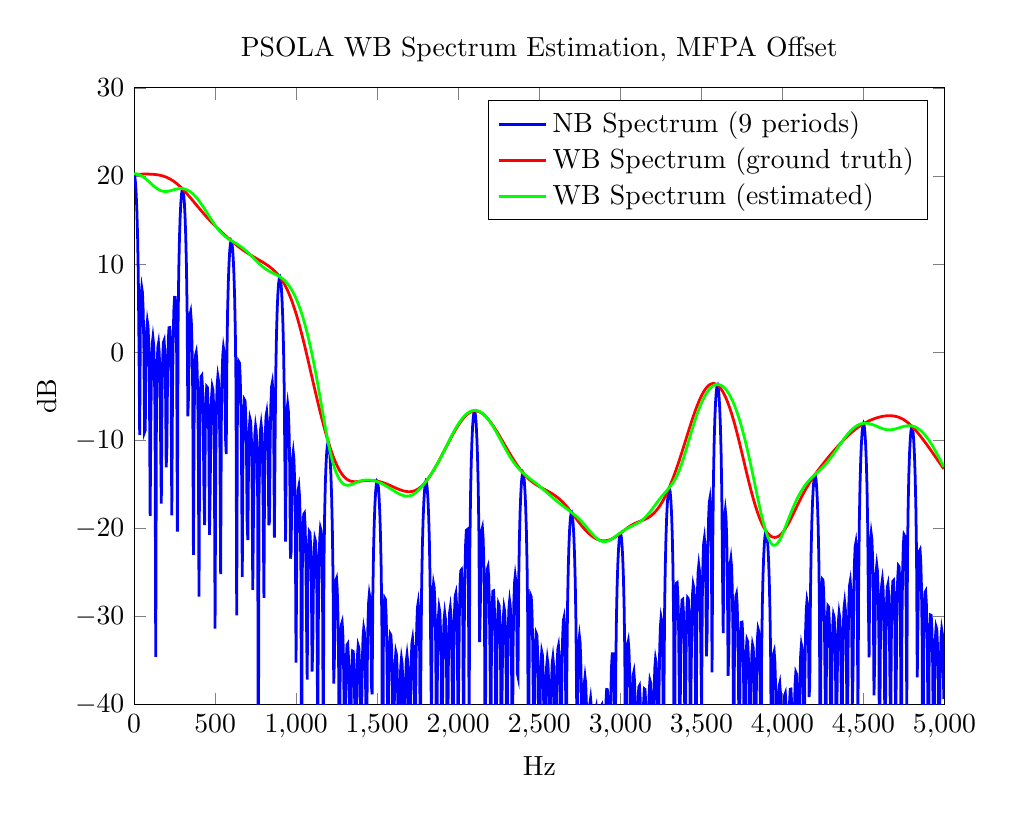
\begin{tikzpicture}

\begin{axis}[%
width=4.052in,
height=3.084in,
at={(0.68in,0.416in)},
scale only axis,
xmin=0,
xmax=5000,
xlabel={Hz},
ymin=-40,
ymax=30,
ylabel={dB},
axis background/.style={fill=white},
title={PSOLA WB Spectrum Estimation, MFPA Offset},
legend style={legend cell align=left,align=left,legend plot pos=left,draw=black}
]
\addplot [color=blue,solid,line width=1.0pt]
  table[row sep=crcr]{%
0	20.1998112835222\\
4.306640625	19.9630253688939\\
8.61328125	19.2360845575318\\
12.919921875	17.9633168361555\\
17.2265625	16.0268836225403\\
21.533203125	13.180537695682\\
25.83984375	8.82254699381025\\
30.146484375	0.700132969808097\\
34.453125	-9.38373028135972\\
38.759765625	2.98659328058475\\
43.06640625	6.33169751815378\\
47.373046875	7.30266913618077\\
51.6796875	6.77667164223539\\
55.986328125	4.80429815421497\\
60.29296875	0.750174864059773\\
64.599609375	-9.06739986575636\\
68.90625	-8.84633812663461\\
73.212890625	-0.448845833559547\\
77.51953125	2.5403005536744\\
81.826171875	3.47160202128536\\
86.1328125	2.92848316932768\\
90.439453125	0.823665076872224\\
94.74609375	-3.79589942490457\\
99.052734375	-18.5756773333599\\
103.359375	-7.93671108111667\\
107.666015625	-1.59488202972874\\
111.97265625	0.938574790851837\\
116.279296875	1.65231303930877\\
120.5859375	0.911077829630306\\
124.892578125	-1.52749587117764\\
129.19921875	-7.11592771881383\\
133.505859375	-34.5722812401772\\
137.8125	-6.61373585025094\\
142.119140625	-1.57112851524897\\
146.42578125	0.545998657477225\\
150.732421875	1.00846814542794\\
155.0390625	0.00753024427498389\\
159.345703125	-2.88396851268621\\
163.65234375	-9.97838634972832\\
167.958984375	-17.1927718041873\\
172.265625	-4.78035058609264\\
176.572265625	-0.638401029402439\\
180.87890625	1.12216069547664\\
185.185546875	1.33907375557166\\
189.4921875	0.0523509699633727\\
193.798828125	-3.40616894653224\\
198.10546875	-13.0783607136449\\
202.412109375	-10.8149063853367\\
206.71875	-2.21399351427716\\
211.025390625	1.2932326952125\\
215.33203125	2.78023534109459\\
219.638671875	2.79677833190986\\
223.9453125	1.23710570621143\\
228.251953125	-2.90986314652361\\
232.55859375	-18.5287229748842\\
236.865234375	-5.07437946200521\\
241.171875	1.68146492127122\\
245.478515625	4.82865651916769\\
249.78515625	6.2251383823794\\
254.091796875	6.21700298464575\\
258.3984375	4.54902151417185\\
262.705078125	-0.316094354876905\\
267.01171875	-20.3631341734267\\
271.318359375	3.0575325482516\\
275.625	9.27891427842231\\
279.931640625	12.9384014511283\\
284.23828125	15.3605744062789\\
288.544921875	16.9768834776396\\
292.8515625	17.9772307831562\\
297.158203125	18.4540713750781\\
301.46484375	18.4483724573271\\
305.771484375	17.9654551343891\\
310.078125	16.9768328564373\\
314.384765625	15.4096529514292\\
318.69140625	13.1137629249197\\
322.998046875	9.76421522356002\\
327.3046875	4.48366650833135\\
331.611328125	-7.28779593916486\\
335.91796875	-4.96268408957308\\
340.224609375	1.99861917064307\\
344.53125	4.24016109828537\\
348.837890625	4.56604715190631\\
353.14453125	3.47389454839626\\
357.451171875	0.821822316752798\\
361.7578125	-4.4793399264641\\
366.064453125	-22.9871894100464\\
370.37109375	-7.92767303445529\\
374.677734375	-2.4009077695411\\
378.984375	-0.342290696274627\\
383.291015625	-0.0312863801554487\\
387.59765625	-1.16210097745387\\
391.904296875	-4.03150884435551\\
396.2109375	-10.3064811168369\\
400.517578125	-27.7454720012042\\
404.82421875	-8.96041617777776\\
409.130859375	-4.50057833605844\\
413.4375	-2.76654864977965\\
417.744140625	-2.64331898403537\\
422.05078125	-3.98848799706377\\
426.357421875	-7.29656530604883\\
430.6640625	-15.2784849930523\\
434.970703125	-19.6280359003298\\
439.27734375	-8.99724258837361\\
443.583984375	-5.32514630847748\\
447.890625	-3.90870070723117\\
452.197265625	-4.01131670320744\\
456.50390625	-5.63872381985393\\
460.810546875	-9.55198582122405\\
465.1171875	-20.7180942624329\\
469.423828125	-15.7930568669292\\
473.73046875	-8.16917574371243\\
478.037109375	-5.08890608921028\\
482.34375	-3.95112449656558\\
486.650390625	-4.27886302677546\\
490.95703125	-6.22662574650125\\
495.263671875	-10.9467752816124\\
499.5703125	-31.3720854955781\\
503.876953125	-12.3005026495531\\
508.18359375	-6.31416655720202\\
512.490234375	-3.66153375393449\\
516.796875	-2.73342069721742\\
521.103515625	-3.24679935077833\\
525.41015625	-5.52163956819098\\
529.716796875	-11.3416106283318\\
534.0234375	-25.1884263224476\\
538.330078125	-7.88815132235102\\
542.63671875	-2.83702992295379\\
546.943359375	-0.390317992662059\\
551.25	0.506453767531607\\
555.556640625	-0.0166482969133403\\
559.86328125	-2.47547139389485\\
564.169921875	-9.79720344227454\\
568.4765625	-11.5585700714678\\
572.783203125	-0.260917670788041\\
577.08984375	4.80216728799505\\
581.396484375	7.96660497742971\\
585.703125	10.0888756045376\\
590.009765625	11.4884644993177\\
594.31640625	12.3134403650122\\
598.623046875	12.6356434402504\\
602.9296875	12.4829286915673\\
607.236328125	11.8494208999965\\
611.54296875	10.6934370617096\\
615.849609375	8.92126187582147\\
620.15625	6.34018611552969\\
624.462890625	2.51060127598473\\
628.76953125	-3.93058726765696\\
633.076171875	-29.8765921370504\\
637.3828125	-7.22073387554979\\
641.689453125	-2.58802074239123\\
645.99609375	-1.08406020592237\\
650.302734375	-1.22451821675793\\
654.609375	-2.76748144168745\\
658.916015625	-6.07369842266098\\
663.22265625	-13.0703615125042\\
667.529296875	-25.4888922745812\\
671.8359375	-10.7681475759189\\
676.142578125	-6.80085219175046\\
680.44921875	-5.37724854639443\\
684.755859375	-5.51878242265869\\
689.0625	-7.1315311122338\\
693.369140625	-10.7845917295229\\
697.67578125	-19.6906547805135\\
701.982421875	-21.331947444522\\
706.2890625	-12.0232587584064\\
710.595703125	-8.70507389456911\\
714.90234375	-7.52962795903941\\
719.208984375	-7.85076038400367\\
723.515625	-9.72012802481867\\
727.822265625	-14.0032074625755\\
732.12890625	-26.9681252466484\\
736.435546875	-18.9683572216046\\
740.7421875	-12.0946118990068\\
745.048828125	-9.31566283462937\\
749.35546875	-8.40778630849761\\
753.662109375	-8.96009418001901\\
757.96875	-11.1765633942772\\
762.275390625	-16.3715606156391\\
766.58203125	-50.4097779235462\\
770.888671875	-16.649390269191\\
775.1953125	-11.2182619719317\\
779.501953125	-8.87541873477621\\
783.80859375	-8.21734155257196\\
788.115234375	-9.01485145668904\\
792.421875	-11.6480762232233\\
796.728515625	-18.1820357938765\\
801.03515625	-27.8814763418916\\
805.341796875	-13.7899449945592\\
809.6484375	-9.29777925877496\\
813.955078125	-7.28269765023121\\
818.26171875	-6.82222429053385\\
822.568359375	-7.84092958267098\\
826.875	-10.9426873551596\\
831.181640625	-19.6363187515666\\
835.48828125	-19.2147076680975\\
839.794921875	-9.70840578203416\\
844.1015625	-5.77334921409505\\
848.408203125	-3.89682282661396\\
852.71484375	-3.46440523501345\\
857.021484375	-4.5384695767372\\
861.328125	-8.0257594005086\\
865.634765625	-21.0448365225365\\
869.94140625	-10.0975056717451\\
874.248046875	-2.195712077007\\
878.5546875	2.03661305204502\\
882.861328125	4.77327991030721\\
887.16796875	6.60322091770327\\
891.474609375	7.76851277988212\\
895.78125	8.38504242800249\\
900.087890625	8.50728188270865\\
904.39453125	8.15087262548289\\
908.701171875	7.2982955639766\\
913.0078125	5.89269374756126\\
917.314453125	3.81429303836856\\
921.62109375	0.812655230261074\\
925.927734375	-3.72703921020973\\
930.234375	-12.1406550808728\\
934.541015625	-21.4830175679408\\
938.84765625	-9.79456922700259\\
943.154296875	-6.68408706564325\\
947.4609375	-5.91921294684327\\
951.767578125	-6.65127897304316\\
956.07421875	-8.84128343273207\\
960.380859375	-13.1459599848905\\
964.6875	-23.4280461085132\\
968.994140625	-22.709719872331\\
973.30078125	-14.7526519311194\\
977.607421875	-12.0393831716497\\
981.9140625	-11.3674018549286\\
986.220703125	-12.1729621553081\\
990.52734375	-14.554974476215\\
994.833984375	-19.4978085436939\\
999.140625	-35.2394625173893\\
1003.447265625	-23.7992519007091\\
1007.75390625	-17.8583238819868\\
1012.060546875	-15.6433421617602\\
1016.3671875	-15.237997396714\\
1020.673828125	-16.2922529627976\\
1024.98046875	-19.0614079921665\\
1029.287109375	-25.0486132711531\\
1033.59375	-49.0489298744527\\
1037.900390625	-24.8089499761534\\
1042.20703125	-20.1642092960551\\
1046.513671875	-18.3960011512\\
1050.8203125	-18.2748293831415\\
1055.126953125	-19.6214733178922\\
1059.43359375	-22.8791188728092\\
1063.740234375	-30.4530193089661\\
1068.046875	-37.1668211819933\\
1072.353515625	-25.5193434711999\\
1076.66015625	-21.7657194537968\\
1080.966796875	-20.3597785467106\\
1085.2734375	-20.4901021210194\\
1089.580078125	-22.127753296442\\
1093.88671875	-25.9629911891354\\
1098.193359375	-36.246288353504\\
1102.5	-33.579043475189\\
1106.806640625	-25.4932347862979\\
1111.11328125	-22.3449523604847\\
1115.419921875	-21.1911146165028\\
1119.7265625	-21.5004356503055\\
1124.033203125	-23.3902174237449\\
1128.33984375	-27.9048897074595\\
1132.646484375	-44.7102230597605\\
1136.953125	-30.2833775016506\\
1141.259765625	-23.9262840157376\\
1145.56640625	-21.0912950068375\\
1149.873046875	-19.9863411636628\\
1154.1796875	-20.279564559475\\
1158.486328125	-22.2395319531199\\
1162.79296875	-27.4586537681424\\
1167.099609375	-45.5842743246826\\
1171.40625	-24.2089204093871\\
1175.712890625	-18.2949510731541\\
1180.01953125	-14.8851512980094\\
1184.326171875	-12.691793179793\\
1188.6328125	-11.2912626612358\\
1192.939453125	-10.4963177591208\\
1197.24609375	-10.2156703212552\\
1201.552734375	-10.4090021409064\\
1205.859375	-11.0714974932495\\
1210.166015625	-12.2322431141108\\
1214.47265625	-13.9650961185263\\
1218.779296875	-16.4223268513851\\
1223.0859375	-19.9344917157253\\
1227.392578125	-25.4005568635528\\
1231.69921875	-37.6231868881101\\
1236.005859375	-34.6680737629009\\
1240.3125	-27.994825560824\\
1244.619140625	-25.8959841344629\\
1248.92578125	-25.683528706939\\
1253.232421875	-26.8777749478328\\
1257.5390625	-29.6326456080537\\
1261.845703125	-35.0734362938085\\
1266.15234375	-54.8514097573601\\
1270.458984375	-38.2663073589712\\
1274.765625	-32.8892469234498\\
1279.072265625	-30.8979252819675\\
1283.37890625	-30.6323479254595\\
1287.685546875	-31.8008987748611\\
1291.9921875	-34.7145473825549\\
1296.298828125	-41.1009369688574\\
1300.60546875	-56.9684224491254\\
1304.912109375	-39.3767009237428\\
1309.21875	-34.9724360950563\\
1313.525390625	-33.2423355395328\\
1317.83203125	-33.1077098181897\\
1322.138671875	-34.4384930600509\\
1326.4453125	-37.7474979121764\\
1330.751953125	-45.8624166843514\\
1335.05859375	-49.4140706504964\\
1339.365234375	-39.0528066719654\\
1343.671875	-35.3738318088744\\
1347.978515625	-33.9175038023049\\
1352.28515625	-33.9714153074006\\
1356.591796875	-35.5531776289137\\
1360.8984375	-39.4494940305821\\
1365.205078125	-50.9154625398585\\
1369.51171875	-45.1326337947302\\
1373.818359375	-37.5949215377083\\
1378.125	-34.4764153065035\\
1382.431640625	-33.2801179057106\\
1386.73828125	-33.5465690198466\\
1391.044921875	-35.442810828673\\
1395.3515625	-40.1602796322515\\
1399.658203125	-62.3297224810393\\
1403.96484375	-40.9954863426594\\
1408.271484375	-35.0323309007632\\
1412.578125	-32.3354466062052\\
1416.884765625	-31.3511525962668\\
1421.19140625	-31.8101434649747\\
1425.498046875	-34.046959405141\\
1429.8046875	-39.9115330777737\\
1434.111328125	-52.4321846741827\\
1438.41796875	-35.9521220254251\\
1442.724609375	-30.9035515648031\\
1447.03125	-28.4187098024568\\
1451.337890625	-27.4766849716494\\
1455.64453125	-27.9592258329553\\
1459.951171875	-30.4009573586294\\
1464.2578125	-37.8600226117026\\
1468.564453125	-38.8379538202033\\
1472.87109375	-27.7690945672026\\
1477.177734375	-22.699252507885\\
1481.484375	-19.4999587165494\\
1485.791015625	-17.3350331009931\\
1490.09765625	-15.8904446411636\\
1494.404296875	-15.0202858544826\\
1498.7109375	-14.6538325756486\\
1503.017578125	-14.763980876241\\
1507.32421875	-15.3572926702582\\
1511.630859375	-16.4763102847611\\
1515.9375	-18.2161636858893\\
1520.244140625	-20.7725504988485\\
1524.55078125	-24.593560318074\\
1528.857421875	-31.0824962855242\\
1533.1640625	-60.4598649948022\\
1537.470703125	-33.9555491987503\\
1541.77734375	-29.3921165970853\\
1546.083984375	-27.8964933617719\\
1550.390625	-28.0350725088891\\
1554.697265625	-29.5790381622938\\
1559.00390625	-32.9040089035676\\
1563.310546875	-40.0097778309555\\
1567.6171875	-51.3457965177724\\
1571.923828125	-37.3078224679822\\
1576.23046875	-33.3955540299073\\
1580.537109375	-31.9889397035259\\
1584.84375	-32.1406957438218\\
1589.150390625	-33.7684943613522\\
1593.45703125	-37.461074618364\\
1597.763671875	-46.5793964602232\\
1602.0703125	-47.5026766593959\\
1606.376953125	-38.4446636874249\\
1610.68359375	-35.1711415105569\\
1614.990234375	-34.0147420882645\\
1619.296875	-34.3504665004912\\
1623.603515625	-36.2413845084006\\
1627.91015625	-40.5813332190181\\
1632.216796875	-54.0586877968533\\
1636.5234375	-45.1511662193199\\
1640.830078125	-38.4103418998207\\
1645.13671875	-35.6618951858327\\
1649.443359375	-34.765945852533\\
1653.75	-35.3272437045274\\
1658.056640625	-37.5623193933281\\
1662.36328125	-42.8305154979651\\
1666.669921875	-104.975649309368\\
1670.9765625	-42.7176261684347\\
1675.283203125	-37.3554006713557\\
1679.58984375	-35.0202604587396\\
1683.896484375	-34.3553669793566\\
1688.203125	-35.1442114329868\\
1692.509765625	-37.7822420781882\\
1696.81640625	-44.4144001495545\\
1701.123046875	-53.1280943956726\\
1705.4296875	-39.557383620042\\
1709.736328125	-35.0795141923781\\
1714.04296875	-33.0373838420722\\
1718.349609375	-32.537675104167\\
1722.65625	-33.5163269255627\\
1726.962890625	-36.5977631423763\\
1731.26953125	-45.4597924187348\\
1735.576171875	-44.2477100992935\\
1739.8828125	-34.8845159778428\\
1744.189453125	-30.9041931763623\\
1748.49609375	-28.9515049463273\\
1752.802734375	-28.4320019136335\\
1757.109375	-29.4194416822271\\
1761.416015625	-32.8506957161765\\
1765.72265625	-46.3693479059954\\
1770.029296875	-34.2808557895966\\
1774.3359375	-26.3628142786716\\
1778.642578125	-22.012212267465\\
1782.94921875	-19.1298878090504\\
1787.255859375	-17.1389723439664\\
1791.5625	-15.8011055204505\\
1795.869140625	-15.0019564760371\\
1800.17578125	-14.6878788442319\\
1804.482421875	-14.8438126989631\\
1808.7890625	-15.4878698935034\\
1813.095703125	-16.6777739056355\\
1817.40234375	-18.5349570979253\\
1821.708984375	-21.3138581276861\\
1826.015625	-25.6425256313867\\
1830.322265625	-33.9442357631557\\
1834.62890625	-42.1597878516606\\
1838.935546875	-30.6691442082378\\
1843.2421875	-27.3358130752316\\
1847.548828125	-26.3048331016152\\
1851.85546875	-26.7550654832247\\
1856.162109375	-28.6590153040817\\
1860.46875	-32.6953363038248\\
1864.775390625	-42.9213312966232\\
1869.08203125	-41.1489301883569\\
1873.388671875	-33.0534286338037\\
1877.6953125	-30.0312904603135\\
1882.001953125	-29.0189732567229\\
1886.30859375	-29.4721500512705\\
1890.615234375	-31.5017047311995\\
1894.921875	-36.1247461605529\\
1899.228515625	-52.2578341102143\\
1903.53515625	-39.257415060976\\
1907.841796875	-33.0260082349903\\
1912.1484375	-30.4289480557643\\
1916.455078125	-29.6194221961028\\
1920.76171875	-30.262464662772\\
1925.068359375	-32.6271824401265\\
1929.375	-38.2703220889431\\
1933.681640625	-59.1053156735768\\
1937.98828125	-36.7723546280088\\
1942.294921875	-31.7508918386798\\
1946.6015625	-29.5519867758319\\
1950.908203125	-28.9868558169204\\
1955.21484375	-29.8891711266675\\
1959.521484375	-32.7195201566249\\
1963.828125	-39.9823078447383\\
1968.134765625	-45.4239550221179\\
1972.44140625	-33.7083735260088\\
1976.748046875	-29.5421199220567\\
1981.0546875	-27.6922591596885\\
1985.361328125	-27.373922383357\\
1989.66796875	-28.5702431157747\\
1993.974609375	-31.9952016286193\\
1998.28125	-42.1255368344246\\
2002.587890625	-38.2680387530637\\
2006.89453125	-29.9185333260343\\
2011.201171875	-26.3667689335384\\
2015.5078125	-24.7931589442721\\
2019.814453125	-24.6852642225431\\
2024.12109375	-26.1727921058266\\
2028.427734375	-30.3354640337953\\
2032.734375	-47.7581845535017\\
2037.041015625	-31.523196112068\\
2041.34765625	-24.876446907335\\
2045.654296875	-21.6822384967924\\
2049.9609375	-20.2118969681157\\
2054.267578125	-20.1480821852721\\
2058.57421875	-21.7734467574225\\
2062.880859375	-26.7385880562228\\
2067.1875	-42.708700428162\\
2071.494140625	-22.4378312304649\\
2075.80078125	-16.268347544036\\
2080.107421875	-12.5651348389637\\
2084.4140625	-10.0764442180625\\
2088.720703125	-8.38683419825366\\
2093.02734375	-7.31216979394629\\
2097.333984375	-6.7627752268266\\
2101.640625	-6.69940453707979\\
2105.947265625	-7.11814163178113\\
2110.25390625	-8.04903307402283\\
2114.560546875	-9.56726083744622\\
2118.8671875	-11.8275001917677\\
2123.173828125	-15.1662322951206\\
2127.48046875	-20.5049129293377\\
2131.787109375	-32.9100769045871\\
2136.09375	-29.0395782303147\\
2140.400390625	-22.3989845730526\\
2144.70703125	-20.216793504205\\
2149.013671875	-19.9144194854456\\
2153.3203125	-21.0295818274495\\
2157.626953125	-23.7281883666489\\
2161.93359375	-29.1728089073116\\
2166.240234375	-50.3589227083544\\
2170.546875	-31.9000210182524\\
2174.853515625	-26.5942818768441\\
2179.16015625	-24.6152615654851\\
2183.466796875	-24.3604339158489\\
2187.7734375	-25.5516873228188\\
2192.080078125	-28.5139349482537\\
2196.38671875	-35.0378142404274\\
2200.693359375	-49.554029092935\\
2205	-33.0309637153544\\
2209.306640625	-28.7545838765739\\
2213.61328125	-27.1184416954249\\
2217.919921875	-27.0782027772328\\
2222.2265625	-28.5153083048277\\
2226.533203125	-31.9605190444566\\
2230.83984375	-40.3646109213481\\
2235.146484375	-43.2906400808699\\
2239.453125	-33.3493502412746\\
2243.759765625	-29.8439687825046\\
2248.06640625	-28.5387648225808\\
2252.373046875	-28.7439277105515\\
2256.6796875	-30.4880394813397\\
2260.986328125	-34.5832900040212\\
2265.29296875	-46.5990097123003\\
2269.599609375	-40.1606439750171\\
2273.90625	-32.9316172930479\\
2278.212890625	-30.0067637592205\\
2282.51953125	-28.9867621626858\\
2286.826171875	-29.4284880457928\\
2291.1328125	-31.5108852154617\\
2295.439453125	-36.4652544837721\\
2299.74609375	-61.2066593100598\\
2304.052734375	-37.2553728178305\\
2308.359375	-31.5458712771851\\
2312.666015625	-29.035643615261\\
2316.97265625	-28.2236888746236\\
2321.279296875	-28.8538076898643\\
2325.5859375	-31.2750064812107\\
2329.892578125	-37.4064015955918\\
2334.19921875	-48.9209090606158\\
2338.505859375	-33.3616871250172\\
2342.8125	-28.5190609187449\\
2347.119140625	-26.1964438496571\\
2351.42578125	-25.405220410786\\
2355.732421875	-26.0387521508391\\
2360.0390625	-28.6507573839285\\
2364.345703125	-36.4386239401824\\
2368.65234375	-36.8163491943689\\
2372.958984375	-26.1301111832324\\
2377.265625	-21.2175341126822\\
2381.572265625	-18.142535171817\\
2385.87890625	-16.0884878695765\\
2390.185546875	-14.7466392148609\\
2394.4921875	-13.9731773329578\\
2398.798828125	-13.6984663538312\\
2403.10546875	-13.8961398044653\\
2407.412109375	-14.5734375108637\\
2411.71875	-15.7737572192914\\
2416.025390625	-17.5936551150677\\
2420.33203125	-20.2318764371414\\
2424.638671875	-24.1452343518514\\
2428.9453125	-30.7789852175617\\
2433.251953125	-66.4019714005567\\
2437.55859375	-33.4074736682387\\
2441.865234375	-28.987962257558\\
2446.171875	-27.5724058903906\\
2450.478515625	-27.7760166309201\\
2454.78515625	-29.3830933938643\\
2459.091796875	-32.7846132055057\\
2463.3984375	-40.0568646178564\\
2467.705078125	-50.4272465723129\\
2472.01171875	-37.0441163688065\\
2476.318359375	-33.2257025076207\\
2480.625	-31.8728563210116\\
2484.931640625	-32.0688774796672\\
2489.23828125	-33.7433360633389\\
2493.544921875	-37.5054889999806\\
2497.8515625	-46.8750563107116\\
2502.158203125	-47.1081249117755\\
2506.46484375	-38.3111303772849\\
2510.771484375	-35.1047564400771\\
2515.078125	-33.9902587211159\\
2519.384765625	-34.3636517375759\\
2523.69140625	-36.2998882110528\\
2527.998046875	-40.7225502599253\\
2532.3046875	-54.7896259723685\\
2536.611328125	-44.9542860085908\\
2540.91796875	-38.3705088203463\\
2545.224609375	-35.6840327972781\\
2549.53125	-34.8350881342123\\
2553.837890625	-35.4442094639198\\
2558.14453125	-37.7410973198588\\
2562.451171875	-43.1324081573405\\
2566.7578125	-76.1903742019872\\
2571.064453125	-42.7385826262528\\
2575.37109375	-37.5061328476314\\
2579.677734375	-35.2482304782899\\
2583.984375	-34.6533440754984\\
2588.291015625	-35.5179554296034\\
2592.59765625	-38.2536050675571\\
2596.904296875	-45.0898161596529\\
2601.2109375	-52.9737074838001\\
2605.517578125	-39.9911606084764\\
2609.82421875	-35.6541297611105\\
2614.130859375	-33.7228341105146\\
2618.4375	-33.3326144968328\\
2622.744140625	-34.431166579502\\
2627.05078125	-37.6644405259101\\
2631.357421875	-46.891886904165\\
2635.6640625	-45.0820004386549\\
2639.970703125	-36.0577487702048\\
2644.27734375	-32.2516534925379\\
2648.583984375	-30.456208457312\\
2652.890625	-30.0967095589726\\
2657.197265625	-31.2586116410841\\
2661.50390625	-34.9101754842159\\
2665.810546875	-49.2903420505588\\
2670.1171875	-36.2939839737482\\
2674.423828125	-28.6721665421373\\
2678.73046875	-24.5341727714305\\
2683.037109375	-21.8517686865512\\
2687.34375	-20.0597004739853\\
2691.650390625	-18.9230923415622\\
2695.95703125	-18.3289537736819\\
2700.263671875	-18.2242397382096\\
2704.5703125	-18.5942402492394\\
2708.876953125	-19.4574264964143\\
2713.18359375	-20.8721590766889\\
2717.490234375	-22.9613131717362\\
2721.796875	-25.9831650620963\\
2726.103515625	-30.5791306822711\\
2730.41015625	-39.2645015623732\\
2734.716796875	-46.8868912081727\\
2739.0234375	-36.0683906140521\\
2743.330078125	-33.0340079398172\\
2747.63671875	-32.2705155956855\\
2751.943359375	-32.983141617458\\
2756.25	-35.1555622573567\\
2760.556640625	-39.4886561707437\\
2764.86328125	-50.2490157418892\\
2769.169921875	-47.9977935954882\\
2773.4765625	-40.3451102434544\\
2777.783203125	-37.6128311072676\\
2782.08984375	-36.8675804163977\\
2786.396484375	-37.5835646475393\\
2790.703125	-39.8832746168773\\
2795.009765625	-44.8172531012501\\
2799.31640625	-62.0877268366828\\
2803.623046875	-48.0597883289766\\
2807.9296875	-42.1796095214999\\
2812.236328125	-39.850498316468\\
2816.54296875	-39.2913922967276\\
2820.849609375	-40.181558693505\\
2825.15625	-42.8034887160782\\
2829.462890625	-48.7692269644519\\
2833.76953125	-67.6710190603224\\
2838.076171875	-47.3425535143462\\
2842.3828125	-42.6081152478516\\
2846.689453125	-40.6435224122418\\
2850.99609375	-40.2984757190075\\
2855.302734375	-41.4186741297192\\
2859.609375	-44.4817140564073\\
2863.916015625	-52.0960084439547\\
2868.22265625	-56.939576564549\\
2872.529296875	-45.7727514113484\\
2876.8359375	-41.8325635694862\\
2881.142578125	-40.1717222817265\\
2885.44921875	-40.0303520492362\\
2889.755859375	-41.402890184059\\
2894.0625	-45.0269874700971\\
2898.369140625	-55.6237059565789\\
2902.67578125	-51.1512579611434\\
2906.982421875	-43.106376082989\\
2911.2890625	-39.7154560459105\\
2915.595703125	-38.2746719849119\\
2919.90234375	-38.2893844680599\\
2924.208984375	-39.9011946186281\\
2928.515625	-44.2258187205749\\
2932.822265625	-62.9494539894544\\
2937.12890625	-45.20416419073\\
2941.435546875	-38.7302720219932\\
2945.7421875	-35.6264854791727\\
2950.048828125	-34.2243062951739\\
2954.35546875	-34.220291840784\\
2958.662109375	-35.9110167472255\\
2962.96875	-41.0075527373224\\
2967.275390625	-55.4321085229669\\
2971.58203125	-36.3630249381074\\
2975.888671875	-30.2626760136278\\
2980.1953125	-26.5734731289619\\
2984.501953125	-24.078095669258\\
2988.80859375	-22.3689574290012\\
2993.115234375	-21.2649081185316\\
2997.421875	-20.6778419447195\\
3001.728515625	-20.5695944891797\\
3006.03515625	-20.9371997656282\\
3010.341796875	-21.8117530474599\\
3014.6484375	-23.2698926232029\\
3018.955078125	-25.4688899689393\\
3023.26171875	-28.7514749790093\\
3027.568359375	-34.0626002178549\\
3031.875	-46.7567933837926\\
3036.181640625	-42.0140647141125\\
3040.48828125	-35.4435329180323\\
3044.794921875	-33.2047814029782\\
3049.1015625	-32.8229357294588\\
3053.408203125	-33.853055362479\\
3057.71484375	-36.4734686098061\\
3062.021484375	-41.885772554196\\
3066.328125	-64.8001384985309\\
3070.634765625	-44.0256507891853\\
3074.94140625	-38.7036744803229\\
3079.248046875	-36.6377587337947\\
3083.5546875	-36.2807343098695\\
3087.861328125	-37.3681605304621\\
3092.16796875	-40.2395008626668\\
3096.474609375	-46.75175834256\\
3100.78125	-59.8863713418095\\
3105.087890625	-44.1156968253799\\
3109.39453125	-39.7750411909474\\
3113.701171875	-38.0305600785413\\
3118.0078125	-37.8714321790394\\
3122.314453125	-39.1908994264135\\
3126.62109375	-42.5385019620826\\
3130.927734375	-50.996269243384\\
3135.234375	-53.0517320032755\\
3139.541015625	-43.2478666730607\\
3143.84765625	-39.6420742745509\\
3148.154296875	-38.2063564403349\\
3152.4609375	-38.27326957514\\
3156.767578125	-39.8828059491262\\
3161.07421875	-43.8738874749665\\
3165.380859375	-56.1615792805698\\
3169.6875	-48.7221387693273\\
3173.994140625	-41.4716201956768\\
3178.30078125	-38.4104877986395\\
3182.607421875	-37.232334849377\\
3186.9140625	-37.5104322603686\\
3191.220703125	-39.4361475502621\\
3195.52734375	-44.2826065316391\\
3199.833984375	-72.3506328331899\\
3204.140625	-44.3239033174075\\
3208.447265625	-38.508211668137\\
3212.75390625	-35.8248824814399\\
3217.060546875	-34.8237049563143\\
3221.3671875	-35.261700656896\\
3225.673828125	-37.5028864137859\\
3229.98046875	-43.5392487927682\\
3234.287109375	-53.7643667312617\\
3238.59375	-38.6700987201614\\
3242.900390625	-33.6625174686423\\
3247.20703125	-31.1321120878291\\
3251.513671875	-30.1216839461902\\
3255.8203125	-30.5363663846188\\
3260.126953125	-32.949699653548\\
3264.43359375	-40.7078270498552\\
3268.740234375	-40.1211212656282\\
3273.046875	-29.4343011190198\\
3277.353515625	-24.3111897390541\\
3281.66015625	-20.9948615767834\\
3285.966796875	-18.6877990173082\\
3290.2734375	-17.0865656035023\\
3294.580078125	-16.0495393873017\\
3298.88671875	-15.5082678115976\\
3303.193359375	-15.437209479094\\
3307.5	-15.8443631517951\\
3311.806640625	-16.7740590742392\\
3316.11328125	-18.3243586101523\\
3320.419921875	-20.6971585827839\\
3324.7265625	-24.3582545035936\\
3329.033203125	-30.7966632455941\\
3333.33984375	-87.898308503967\\
3337.646484375	-32.5023850324611\\
3341.953125	-27.8882052865314\\
3346.259765625	-26.2187432694613\\
3350.56640625	-26.1560297487135\\
3354.873046875	-27.4972729398102\\
3359.1796875	-30.6490528995852\\
3363.486328125	-37.7680234425667\\
3367.79296875	-46.9060882406758\\
3372.099609375	-33.7968149279235\\
3376.40625	-29.7516183777346\\
3380.712890625	-28.1349599333455\\
3385.01953125	-28.0596503708899\\
3389.326171875	-29.467031045515\\
3393.6328125	-32.9873491078435\\
3397.939453125	-42.3101800080251\\
3402.24609375	-41.5434651589063\\
3406.552734375	-32.6866965230436\\
3410.859375	-29.2399168429454\\
3415.166015625	-27.8619762418519\\
3419.47265625	-27.969367348393\\
3423.779296875	-29.6489764186699\\
3428.0859375	-33.8551250672344\\
3432.392578125	-48.2737978570864\\
3436.69921875	-37.155285439225\\
3441.005859375	-30.4269835467674\\
3445.3125	-27.5067787922715\\
3449.619140625	-26.4111293040105\\
3453.92578125	-26.7760731970912\\
3458.232421875	-28.8446485372534\\
3462.5390625	-34.0727954023431\\
3466.845703125	-60.8312370801053\\
3471.15234375	-32.8238852301067\\
3475.458984375	-27.433849934354\\
3479.765625	-24.9693002744062\\
3484.072265625	-24.1622093019711\\
3488.37890625	-24.8218552108221\\
3492.685546875	-27.3761422467702\\
3496.9921875	-34.1436421553486\\
3501.298828125	-40.9591739816712\\
3505.60546875	-28.2447451098672\\
3509.912109375	-23.7716761263398\\
3514.21875	-21.6764462723872\\
3518.525390625	-21.1221008386829\\
3522.83203125	-22.0680036202678\\
3527.138671875	-25.1821726879801\\
3531.4453125	-34.5192444999425\\
3535.751953125	-31.8361391692179\\
3540.05859375	-22.8701351695767\\
3544.365234375	-18.9681762457944\\
3548.671875	-17.0613476497315\\
3552.978515625	-16.5942517106421\\
3557.28515625	-17.6641790056877\\
3561.591796875	-21.271977885647\\
3565.8984375	-36.3384391390482\\
3570.205078125	-22.0843768220444\\
3574.51171875	-14.4923292148138\\
3578.818359375	-10.3061560656329\\
3583.125	-7.56547146462717\\
3587.431640625	-5.71671307315549\\
3591.73828125	-4.5288711563796\\
3596.044921875	-3.89076794039449\\
3600.3515625	-3.75047469524362\\
3604.658203125	-4.09416604142618\\
3608.96484375	-4.94121195811794\\
3613.271484375	-6.35114635341578\\
3617.578125	-8.44882395653159\\
3621.884765625	-11.496936074289\\
3626.19140625	-16.1511483228959\\
3630.498046875	-25.0244772708826\\
3634.8046875	-31.8867059962897\\
3639.111328125	-21.5214674090735\\
3643.41796875	-18.6076776165396\\
3647.724609375	-17.9436675380155\\
3652.03125	-18.7606058249232\\
3656.337890625	-21.0536835829067\\
3660.64453125	-25.5469853120076\\
3664.951171875	-36.7334938812177\\
3669.2578125	-33.8773788511342\\
3673.564453125	-26.5533109935897\\
3677.87109375	-24.0164773362994\\
3682.177734375	-23.4561643115808\\
3686.484375	-24.364838191111\\
3690.791015625	-26.8768173515131\\
3695.09765625	-32.0773934090619\\
3699.404296875	-50.5931716189613\\
3703.7109375	-35.375970378973\\
3708.017578125	-29.8329634357418\\
3712.32421875	-27.7731639324115\\
3716.630859375	-27.4781512387855\\
3720.9375	-28.641033146353\\
3725.244140625	-31.5577057211767\\
3729.55078125	-37.8977975230265\\
3733.857421875	-55.2812532811887\\
3738.1640625	-36.6704044693151\\
3742.470703125	-32.3014494149929\\
3746.77734375	-30.6615062142649\\
3751.083984375	-30.6369844289146\\
3755.390625	-32.0851180008102\\
3759.697265625	-35.5005042273147\\
3764.00390625	-43.6012611473214\\
3768.310546875	-48.0012627869981\\
3772.6171875	-37.5008205229226\\
3776.923828125	-33.9362508635276\\
3781.23046875	-32.6220178233208\\
3785.537109375	-32.822130126578\\
3789.84375	-34.5419603726996\\
3794.150390625	-38.5431782861696\\
3798.45703125	-49.8119539462272\\
3802.763671875	-44.8962245483157\\
3807.0703125	-37.3404272582706\\
3811.376953125	-34.3065508952583\\
3815.68359375	-33.1996908850795\\
3819.990234375	-33.5423154561426\\
3824.296875	-35.4877507046427\\
3828.603515625	-40.1888042178531\\
3832.91015625	-60.6868533208456\\
3837.216796875	-41.39379337141\\
3841.5234375	-35.3105491477842\\
3845.830078125	-32.5206145148892\\
3850.13671875	-31.4128202790261\\
3854.443359375	-31.6971938643931\\
3858.75	-33.6842398486729\\
3863.056640625	-39.1480971376655\\
3867.36328125	-52.4386834415479\\
3871.669921875	-34.6258237517792\\
3875.9765625	-28.8280826027843\\
3880.283203125	-25.3883670018722\\
3884.58984375	-23.1220693136767\\
3888.896484375	-21.6288175154311\\
3893.203125	-20.7299072326356\\
3897.509765625	-20.33826943484\\
3901.81640625	-20.4162825087401\\
3906.123046875	-20.9613913740309\\
3910.4296875	-22.0052094866458\\
3914.736328125	-23.625321246784\\
3919.04296875	-25.9811257412618\\
3923.349609375	-29.4212517010787\\
3927.65625	-34.9144985488446\\
3931.962890625	-48.1301517939177\\
3936.26953125	-42.688807619025\\
3940.576171875	-36.3720288025237\\
3944.8828125	-34.2599165531544\\
3949.189453125	-33.9753835547092\\
3953.49609375	-35.0901615566207\\
3957.802734375	-37.7948626624207\\
3962.109375	-43.3314065871638\\
3966.416015625	-68.7233902463632\\
3970.72265625	-45.1698694300168\\
3975.029296875	-39.9587219586994\\
3979.3359375	-37.9276930197624\\
3983.642578125	-37.5827082075015\\
3987.94921875	-38.6729362954293\\
3992.255859375	-41.5528365952521\\
3996.5625	-48.1492493356854\\
4000.869140625	-60.0919194311006\\
4005.17578125	-45.0433671452409\\
4009.482421875	-40.7081805705343\\
4013.7890625	-38.9208743767447\\
4018.095703125	-38.7035787727377\\
4022.40234375	-39.9619045651966\\
4026.708984375	-43.265330991318\\
4031.015625	-51.8363666589229\\
4035.322265625	-53.0754786121504\\
4039.62890625	-43.4379821518067\\
4043.935546875	-39.7758260182943\\
4048.2421875	-38.2547323736207\\
4052.548828125	-38.229874431845\\
4056.85546875	-39.7535475691503\\
4061.162109375	-43.6931223978237\\
4065.46875	-56.3461892477851\\
4069.775390625	-47.9316970843081\\
4074.08203125	-40.7181773106783\\
4078.388671875	-37.5905987623993\\
4082.6953125	-36.3313455051121\\
4087.001953125	-36.5303896757073\\
4091.30859375	-38.3922550156488\\
4095.615234375	-43.234116820216\\
4099.921875	-77.5919049398064\\
4104.228515625	-42.7561984344048\\
4108.53515625	-36.9604380747273\\
4112.841796875	-34.2427988599219\\
4117.1484375	-33.2020882258062\\
4121.455078125	-33.608620692722\\
4125.76171875	-35.841885627184\\
4130.068359375	-41.9705325509056\\
4134.375	-51.1679810891721\\
4138.681640625	-36.6717705453747\\
4142.98828125	-31.7133860218942\\
4147.294921875	-29.2016676846111\\
4151.6015625	-28.2096704400306\\
4155.908203125	-28.6540830580974\\
4160.21484375	-31.1285943315905\\
4164.521484375	-39.1380556874425\\
4168.828125	-37.8683400911948\\
4173.134765625	-27.4560839575006\\
4177.44140625	-22.4200931090986\\
4181.748046875	-19.1702080430285\\
4186.0546875	-16.9271646060258\\
4190.361328125	-15.3924780794908\\
4194.66796875	-14.4264335794054\\
4198.974609375	-13.9615033212945\\
4203.28125	-13.9727234892349\\
4207.587890625	-14.468611492929\\
4211.89453125	-15.4941969487991\\
4216.201171875	-17.1488258695487\\
4220.5078125	-19.6373635981454\\
4224.814453125	-23.4345787463369\\
4229.12109375	-30.0748967364654\\
4233.427734375	-63.8869409046795\\
4237.734375	-31.6658373912448\\
4242.041015625	-27.2672532852973\\
4246.34765625	-25.7619814440799\\
4250.654296875	-25.8567379433016\\
4254.9609375	-27.3611944387761\\
4259.267578125	-30.6975351525389\\
4263.57421875	-38.1066714040916\\
4267.880859375	-46.5009199140183\\
4272.1875	-34.0605247164625\\
4276.494140625	-30.236126113298\\
4280.80078125	-28.8073943374312\\
4285.107421875	-28.9152914713248\\
4289.4140625	-30.5124442775841\\
4293.720703125	-34.2501833507845\\
4298.02734375	-43.9997482977447\\
4302.333984375	-42.690641876449\\
4306.640625	-34.22229218336\\
4310.947265625	-30.9935243077054\\
4315.25390625	-29.8101622636356\\
4319.560546875	-30.1080469517845\\
4323.8671875	-31.9854189248997\\
4328.173828125	-36.4277324462624\\
4332.48046875	-51.7189862525618\\
4336.787109375	-39.6899809716274\\
4341.09375	-33.2502279576903\\
4345.400390625	-30.5277746861758\\
4349.70703125	-29.6110081010706\\
4354.013671875	-30.1505371225332\\
4358.3203125	-32.4022695523056\\
4362.626953125	-37.8728994289332\\
4366.93359375	-61.1166975838226\\
4371.240234375	-36.5463173265365\\
4375.546875	-31.3704599399011\\
4379.853515625	-29.0624621170011\\
4384.16015625	-28.395643370531\\
4388.466796875	-29.1914705790121\\
4392.7734375	-31.8941022845486\\
4397.080078125	-38.9156002828711\\
4401.38671875	-44.9989500525137\\
4405.693359375	-32.8054537546707\\
4410	-28.4719021960101\\
4414.306640625	-26.47554417908\\
4418.61328125	-26.0059731466628\\
4422.919921875	-27.0339147508144\\
4427.2265625	-30.2498147208535\\
4431.533203125	-39.9183607819267\\
4435.83984375	-36.5442599049321\\
4440.146484375	-27.8007302920081\\
4444.453125	-23.9606431446941\\
4448.759765625	-22.085116016838\\
4453.06640625	-21.6374220658491\\
4457.373046875	-22.7265986475699\\
4461.6796875	-26.3870787144713\\
4465.986328125	-42.329887259366\\
4470.29296875	-26.7707156984816\\
4474.599609375	-19.2491342754301\\
4478.90625	-15.0422376130894\\
4483.212890625	-12.2541052225542\\
4487.51953125	-10.3423630730968\\
4491.826171875	-9.0795963835618\\
4496.1328125	-8.3562082189104\\
4500.439453125	-8.12116370252309\\
4504.74609375	-8.36130623536975\\
4509.052734375	-9.09669968333317\\
4513.359375	-10.3878650166745\\
4517.666015625	-12.3614834127136\\
4521.97265625	-15.2845874829959\\
4526.279296875	-19.8273743727231\\
4530.5859375	-28.7061328945881\\
4534.892578125	-34.6221451122058\\
4539.19921875	-24.4531053219265\\
4543.505859375	-21.4112056885833\\
4547.8125	-20.5796366412841\\
4552.119140625	-21.2147220098272\\
4556.42578125	-23.3231775867827\\
4560.732421875	-27.6530273186601\\
4565.0390625	-38.9425767382805\\
4569.345703125	-35.1055753121824\\
4573.65234375	-27.7194705260882\\
4577.958984375	-24.9764684901373\\
4582.265625	-24.181707492025\\
4586.572265625	-24.8458050590187\\
4590.87890625	-27.1153680782757\\
4595.185546875	-32.1121467137223\\
4599.4921875	-51.5724026569041\\
4603.798828125	-34.4742002066132\\
4608.10546875	-28.7434755412787\\
4612.412109375	-26.416422324197\\
4616.71875	-25.8352306375824\\
4621.025390625	-26.7074622824445\\
4625.33203125	-29.3435415433163\\
4629.638671875	-35.4743121890495\\
4633.9453125	-50.9847890287294\\
4638.251953125	-33.2396079963893\\
4642.55859375	-28.6188562031977\\
4646.865234375	-26.6809560102724\\
4651.171875	-26.3489190036625\\
4655.478515625	-27.4926792475698\\
4659.78515625	-30.6255289173982\\
4664.091796875	-38.5832021111196\\
4668.3984375	-41.916795552149\\
4672.705078125	-31.4222113226116\\
4677.01171875	-27.596404018637\\
4681.318359375	-25.9960749874784\\
4685.625	-25.909628421414\\
4689.931640625	-27.3545599046565\\
4694.23828125	-31.1184507772551\\
4698.544921875	-42.477652793943\\
4702.8515625	-36.5002305023374\\
4707.158203125	-28.8370555881157\\
4711.46484375	-25.581331659219\\
4715.771484375	-24.2419866429776\\
4720.078125	-24.3590980174324\\
4724.384765625	-26.098659530333\\
4728.69140625	-30.6527694731462\\
4732.998046875	-52.794777485411\\
4737.3046875	-31.0806997464138\\
4741.611328125	-24.9062961654376\\
4745.91796875	-21.9681674588141\\
4750.224609375	-20.7104687918871\\
4754.53125	-20.8569153064109\\
4758.837890625	-22.7325590355733\\
4763.14453125	-28.177962723032\\
4767.451171875	-40.0977418381313\\
4771.7578125	-23.0524089142858\\
4776.064453125	-17.222693271396\\
4780.37109375	-13.7189446356193\\
4784.677734375	-11.3882639539286\\
4788.984375	-9.83753407324894\\
4793.291015625	-8.89065921707931\\
4797.59765625	-8.46178967574663\\
4801.904296875	-8.51402639424609\\
4806.2109375	-9.0453937397562\\
4810.517578125	-10.0881767940732\\
4814.82421875	-11.7210454262671\\
4819.130859375	-14.105666221705\\
4823.4375	-17.5967838293379\\
4827.744140625	-23.1879510020181\\
4832.05078125	-36.8944864593681\\
4836.357421875	-30.6835479592727\\
4840.6640625	-24.5923760514413\\
4844.970703125	-22.6057979022391\\
4849.27734375	-22.4392941121155\\
4853.583984375	-23.6808422413688\\
4857.890625	-26.533355954609\\
4862.197265625	-32.2805130334332\\
4866.50390625	-61.3911772198352\\
4870.810546875	-34.0483647868455\\
4875.1171875	-29.0903536544077\\
4879.423828125	-27.2589678595479\\
4883.73046875	-27.110635491222\\
4888.037109375	-28.4075051551957\\
4892.34375	-31.5187941372004\\
4896.650390625	-38.4440523030812\\
4900.95703125	-49.5358244093283\\
4905.263671875	-35.3966788182246\\
4909.5703125	-31.3551008544895\\
4913.876953125	-29.8294767479422\\
4918.18359375	-29.8728799714812\\
4922.490234375	-31.4022401996396\\
4926.796875	-35.0064212594587\\
4931.103515625	-44.0566037331007\\
4935.41015625	-44.8485436957538\\
4939.716796875	-35.7354362738379\\
4944.0234375	-32.3965138666402\\
4948.330078125	-31.1766006455004\\
4952.63671875	-31.4516423281939\\
4956.943359375	-33.2850109850823\\
4961.25	-37.5721775922188\\
4965.556640625	-51.0340132873053\\
4969.86328125	-42.0032084716122\\
4974.169921875	-35.2184504886396\\
4978.4765625	-32.4189162313148\\
4982.783203125	-31.4702887522931\\
4987.08984375	-31.9779635562361\\
4991.396484375	-34.1588730064248\\
4995.703125	-39.3751820424122\\
};
\addlegendentry{NB Spectrum (9 periods)};

\addplot [color=red,solid,line width=1.0pt]
  table[row sep=crcr]{%
0	20.1998112835222\\
4.306640625	20.1999011742825\\
8.61328125	20.2001691995733\\
12.919921875	20.2006103105267\\
17.2265625	20.2012157743361\\
21.533203125	20.201972828705\\
25.83984375	20.2028644145719\\
30.146484375	20.2038691110386\\
34.453125	20.2049613351258\\
38.759765625	20.2061117844833\\
43.06640625	20.2072880219475\\
47.373046875	20.2084550540905\\
51.6796875	20.2095757585421\\
55.986328125	20.2106110676231\\
60.29296875	20.2115199026489\\
64.599609375	20.2122589461967\\
68.90625	20.2127824076396\\
73.212890625	20.2130419562457\\
77.51953125	20.2129869569652\\
81.826171875	20.2125650558917\\
86.1328125	20.2117230504754\\
90.439453125	20.2104078776079\\
94.74609375	20.2085674926843\\
99.052734375	20.2061514150257\\
103.359375	20.2031107818572\\
107.666015625	20.1993978675746\\
111.97265625	20.1949651561304\\
116.279296875	20.1897641656757\\
120.5859375	20.1837442851985\\
124.892578125	20.1768518764347\\
129.19921875	20.1690298236526\\
133.505859375	20.160217600056\\
137.8125	20.1503517952631\\
142.119140625	20.1393669481407\\
146.42578125	20.1271964793635\\
150.732421875	20.1137735287114\\
155.0390625	20.0990315653217\\
159.345703125	20.0829047317931\\
163.65234375	20.0653279746769\\
167.958984375	20.0462370763077\\
172.265625	20.0255687188241\\
176.572265625	20.0032606792708\\
180.87890625	19.9792521891537\\
185.185546875	19.9534844175366\\
189.4921875	19.9259009805725\\
193.798828125	19.8964483622049\\
198.10546875	19.8650761572145\\
202.412109375	19.8317371099025\\
206.71875	19.796386998147\\
211.025390625	19.758984476705\\
215.33203125	19.7194910224133\\
219.638671875	19.6778711057262\\
223.9453125	19.6340926516278\\
228.251953125	19.5881277667436\\
232.55859375	19.5399536255628\\
236.865234375	19.4895533542587\\
241.171875	19.4369167439482\\
245.478515625	19.3820406696415\\
249.78515625	19.3249291734407\\
254.091796875	19.2655932651018\\
258.3984375	19.2040505697695\\
262.705078125	19.1403249866337\\
267.01171875	19.0744465019138\\
271.318359375	19.0064512308124\\
275.625	18.9363816676112\\
279.931640625	18.8642870317693\\
284.23828125	18.7902235409454\\
288.544921875	18.714254439067\\
292.8515625	18.6364496616496\\
297.158203125	18.5568851159855\\
301.46484375	18.4756416614212\\
305.771484375	18.3928039610457\\
310.078125	18.3084594132177\\
314.384765625	18.2226973470167\\
318.69140625	18.1356085866331\\
322.998046875	18.0472853798489\\
327.3046875	17.9578215786195\\
331.611328125	17.8673128878436\\
335.91796875	17.7758569827256\\
340.224609375	17.683553338762\\
344.53125	17.5905027056763\\
348.837890625	17.4968062587574\\
353.14453125	17.4025645457044\\
357.451171875	17.3078763891486\\
361.7578125	17.212837894784\\
366.064453125	17.1175416608314\\
370.37109375	17.0220762093432\\
374.677734375	16.9265255926417\\
378.984375	16.8309690935292\\
383.291015625	16.7354809470368\\
387.59765625	16.6401300583536\\
391.904296875	16.544979755171\\
396.2109375	16.4500876648763\\
400.517578125	16.3555058232025\\
404.82421875	16.2612810894567\\
409.130859375	16.1674558706566\\
413.4375	16.0740690655608\\
417.744140625	15.981157061308\\
422.05078125	15.8887545794886\\
426.357421875	15.7968951913528\\
430.6640625	15.7056114005022\\
434.970703125	15.6149343036914\\
439.27734375	15.5248929519666\\
443.583984375	15.4355136101613\\
447.890625	15.346819128735\\
452.197265625	15.2588285934395\\
456.50390625	15.1715573218286\\
460.810546875	15.0850171633433\\
465.1171875	14.9992169684717\\
469.423828125	14.9141630514137\\
473.73046875	14.8298594912764\\
478.037109375	14.7463081893851\\
482.34375	14.6635086976384\\
486.650390625	14.5814579200893\\
490.95703125	14.5001498368473\\
495.263671875	14.4195753908361\\
499.5703125	14.3397226188662\\
503.876953125	14.2605770217843\\
508.18359375	14.1821220863647\\
512.490234375	14.1043398239608\\
516.796875	14.0272111944795\\
521.103515625	13.9507163367966\\
525.41015625	13.8748346082945\\
529.716796875	13.7995445164837\\
534.0234375	13.7248236752578\\
538.330078125	13.6506489193953\\
542.63671875	13.576996663576\\
546.943359375	13.5038435142164\\
551.25	13.4311670625806\\
555.556640625	13.3589467348467\\
559.86328125	13.2871645675512\\
564.169921875	13.2158058162168\\
568.4765625	13.1448593744138\\
572.783203125	13.0743180519156\\
577.08984375	13.0041788048659\\
581.396484375	12.9344430088468\\
585.703125	12.8651168157242\\
590.009765625	12.7962115540932\\
594.31640625	12.7277440510244\\
598.623046875	12.6597367021259\\
602.9296875	12.5922171210999\\
607.236328125	12.5252172645085\\
611.54296875	12.4587720374087\\
615.849609375	12.3929175097616\\
620.15625	12.3276889748202\\
624.462890625	12.2631191278924\\
628.76953125	12.1992366221091\\
633.076171875	12.136065173369\\
637.3828125	12.0736232646099\\
641.689453125	12.0119243754303\\
645.99609375	11.9509775709327\\
650.302734375	11.8907882453244\\
654.609375	11.831358834637\\
658.916015625	11.7726893741851\\
663.22265625	11.714777853794\\
667.529296875	11.6576203897091\\
671.8359375	11.6012112672306\\
676.142578125	11.5455429077808\\
680.44921875	11.4906057883485\\
684.755859375	11.4363883094125\\
689.0625	11.3828765894995\\
693.369140625	11.3300541724434\\
697.67578125	11.2779016660979\\
701.982421875	11.2263963749207\\
706.2890625	11.1755120226785\\
710.595703125	11.1252186663647\\
714.90234375	11.0754828691546\\
719.208984375	11.0262681344345\\
723.515625	10.9775355239695\\
727.822265625	10.9292443178223\\
732.12890625	10.8813525461587\\
736.435546875	10.8338172465079\\
740.7421875	10.7865943703541\\
745.048828125	10.7396383595736\\
749.35546875	10.6929015056337\\
753.662109375	10.6463332622201\\
757.96875	10.5998796853518\\
762.275390625	10.5534831220797\\
766.58203125	10.5070821763987\\
770.888671875	10.4606118793541\\
775.1953125	10.4140039132926\\
779.501953125	10.3671867137342\\
783.80859375	10.320085305821\\
788.115234375	10.2726208153859\\
792.421875	10.2247097007364\\
796.728515625	10.176262846071\\
801.03515625	10.1271847105221\\
805.341796875	10.0773727211029\\
809.6484375	10.0267170351043\\
813.955078125	9.97510069742889\\
818.26171875	9.92240011191808\\
822.568359375	9.86848566501053\\
826.875	9.81322230811222\\
831.181640625	9.75646992893665\\
835.48828125	9.69808341138662\\
839.794921875	9.63791237452777\\
844.1015625	9.5758006649355\\
848.408203125	9.51158572861738\\
852.71484375	9.44509799633513\\
857.021484375	9.37616038262153\\
861.328125	9.30458794127476\\
865.634765625	9.23018766363309\\
869.94140625	9.15275837464629\\
874.248046875	9.07209069052542\\
878.5546875	8.98796705058868\\
882.861328125	8.90016190916542\\
887.16796875	8.80844224392137\\
891.474609375	8.71256857421191\\
895.78125	8.61229666295043\\
900.087890625	8.50737998889429\\
904.39453125	8.39757293388214\\
908.701171875	8.28263446117894\\
913.0078125	8.1623319091862\\
917.314453125	8.03644443388648\\
921.62109375	7.90476563775262\\
925.927734375	7.76710503562941\\
930.234375	7.62328821519304\\
934.541015625	7.47315581019119\\
938.84765625	7.31656165915322\\
943.154296875	7.15337070635854\\
947.4609375	6.98345726381442\\
951.767578125	6.80670416929049\\
956.07421875	6.62300316007286\\
960.380859375	6.43225648582336\\
964.6875	6.23437948265603\\
968.994140625	6.0293036051255\\
973.30078125	5.81697932584821\\
977.607421875	5.59737838893257\\
981.9140625	5.37049512139334\\
986.220703125	5.13634680190808\\
990.52734375	4.89497336944402\\
994.833984375	4.64643693773649\\
999.140625	4.3908216065105\\
1003.447265625	4.12823391658021\\
1007.75390625	3.8588040274731\\
1012.060546875	3.58268738915393\\
1016.3671875	3.30006643579055\\
1020.673828125	3.01115173415757\\
1024.98046875	2.71618211068687\\
1029.287109375	2.41542353608723\\
1033.59375	2.10916688443998\\
1037.900390625	1.79772499141634\\
1042.20703125	1.48142960476511\\
1046.513671875	1.16062878323494\\
1050.8203125	0.835685060526617\\
1055.126953125	0.506974324936499\\
1059.43359375	0.174885001016148\\
1063.740234375	-0.160183105427359\\
1068.046875	-0.497820925086445\\
1072.353515625	-0.837613562410282\\
1076.66015625	-1.17914495754463\\
1080.966796875	-1.52200319463625\\
1085.2734375	-1.86578554114466\\
1089.580078125	-2.2101022555711\\
1093.88671875	-2.55457849469186\\
1098.193359375	-2.89885421551104\\
1102.5	-3.24258262246972\\
1106.806640625	-3.58542822372235\\
1111.11328125	-3.92706572511818\\
1115.419921875	-4.26718070663954\\
1119.7265625	-4.60547234745831\\
1124.033203125	-4.94165759694519\\
1128.33984375	-5.27547542545242\\
1132.646484375	-5.60668941852308\\
1136.953125	-5.93508717656698\\
1141.259765625	-6.26047573786962\\
1145.56640625	-6.5826733474745\\
1149.873046875	-6.90149900259947\\
1154.1796875	-7.21676194929773\\
1158.486328125	-7.52825342417801\\
1162.79296875	-7.8357423705837\\
1167.099609375	-8.13897578112121\\
1171.40625	-8.43768307375292\\
1175.712890625	-8.73158290178894\\
1180.01953125	-9.02039035295387\\
1184.326171875	-9.30382273732562\\
1188.6328125	-9.5816029831214\\
1192.939453125	-9.85346073472956\\
1197.24609375	-10.1191321739992\\
1201.552734375	-10.3783600227195\\
1205.859375	-10.6308949830903\\
1210.166015625	-10.8764991335614\\
1214.47265625	-11.1149508278141\\
1218.779296875	-11.3460498409163\\
1223.0859375	-11.5696211978776\\
1227.392578125	-11.785516439112\\
1231.69921875	-11.993611909784\\
1236.005859375	-12.1938046884024\\
1240.3125	-12.3860076001526\\
1244.619140625	-12.570145075613\\
1248.92578125	-12.7461512978891\\
1253.232421875	-12.9139712532331\\
1257.5390625	-13.0735642720972\\
1261.845703125	-13.224908795159\\
1266.15234375	-13.3680067215075\\
1270.458984375	-13.5028859092482\\
1274.765625	-13.6296000998801\\
1279.072265625	-13.7482264555635\\
1283.37890625	-13.8588617007048\\
1287.685546875	-13.9616182762713\\
1291.9921875	-14.0566218301074\\
1296.298828125	-14.1440108435312\\
1300.60546875	-14.2239384405652\\
1304.912109375	-14.2965757070663\\
1309.21875	-14.362115392897\\
1313.525390625	-14.4207748038222\\
1317.83203125	-14.4727969980507\\
1322.138671875	-14.5184499552047\\
1326.4453125	-14.5580239888804\\
1330.751953125	-14.5918281360886\\
1335.05859375	-14.620186445987\\
1339.365234375	-14.6434349683453\\
1343.671875	-14.6619198679573\\
1347.978515625	-14.675996596602\\
1352.28515625	-14.6860296019481\\
1356.591796875	-14.6923917885638\\
1360.8984375	-14.6954629560735\\
1365.205078125	-14.6956267246513\\
1369.51171875	-14.6932659326513\\
1373.818359375	-14.6887570059984\\
1378.125	-14.6824641852488\\
1382.431640625	-14.6747346184662\\
1386.73828125	-14.6658951297996\\
1391.044921875	-14.656251001099\\
1395.3515625	-14.6460864977928\\
1399.658203125	-14.6356663260034\\
1403.96484375	-14.6252369145577\\
1408.271484375	-14.6150264920694\\
1412.578125	-14.6052433791583\\
1416.884765625	-14.596072617145\\
1421.19140625	-14.587671791303\\
1425.498046875	-14.5801674341761\\
1429.8046875	-14.5736535179075\\
1434.111328125	-14.5681931862893\\
1438.41796875	-14.5638241088885\\
1442.724609375	-14.560566867853\\
1447.03125	-14.5584348968434\\
1451.337890625	-14.5574439570632\\
1455.64453125	-14.557619138486\\
1459.951171875	-14.5589979392033\\
1464.2578125	-14.5616289551861\\
1468.564453125	-14.5655668288225\\
1472.87109375	-14.5708650335848\\
1477.177734375	-14.5775685460842\\
1481.484375	-14.5857083474639\\
1485.791015625	-14.5952990534612\\
1490.09765625	-14.6063400049576\\
1494.404296875	-14.6188191565283\\
1498.7109375	-14.6327183727605\\
1503.017578125	-14.6480184798346\\
1507.32421875	-14.6647026697517\\
1511.630859375	-14.6827575026629\\
1515.9375	-14.7021715669909\\
1520.244140625	-14.7229325670621\\
1524.55078125	-14.7450239948523\\
1528.857421875	-14.7684225080507\\
1533.1640625	-14.7930967295972\\
1537.470703125	-14.8190075747032\\
1541.77734375	-14.8461096279856\\
1546.083984375	-14.8743527400423\\
1550.390625	-14.9036830013459\\
1554.697265625	-14.9340425665639\\
1559.00390625	-14.9653683127853\\
1563.310546875	-14.9975898235519\\
1567.6171875	-15.0306275066822\\
1571.923828125	-15.0643916618971\\
1576.23046875	-15.09878301272\\
1580.537109375	-15.1336947167995\\
1584.84375	-15.1690153510645\\
1589.150390625	-15.2046320192368\\
1593.45703125	-15.2404326739935\\
1597.763671875	-15.2763070040542\\
1602.0703125	-15.3121457159224\\
1606.376953125	-15.3478385714984\\
1610.68359375	-15.3832719403733\\
1614.990234375	-15.4183267533887\\
1619.296875	-15.4528775636577\\
1623.603515625	-15.4867930037912\\
1627.91015625	-15.5199374264995\\
1632.216796875	-15.5521731089129\\
1636.5234375	-15.583362229648\\
1640.830078125	-15.6133679454386\\
1645.13671875	-15.6420542503363\\
1649.443359375	-15.6692847605646\\
1653.75	-15.6949209640863\\
1658.056640625	-15.7188206656235\\
1662.36328125	-15.7408372826417\\
1666.669921875	-15.7608203407702\\
1670.9765625	-15.7786170952634\\
1675.283203125	-15.7940748224399\\
1679.58984375	-15.8070431159224\\
1683.896484375	-15.8173755541648\\
1688.203125	-15.8249303565305\\
1692.509765625	-15.829570015869\\
1696.81640625	-15.8311602484706\\
1701.123046875	-15.8295688129918\\
1705.4296875	-15.82466475183\\
1709.736328125	-15.8163184140753\\
1714.04296875	-15.8044023116778\\
1718.349609375	-15.7887925594533\\
1722.65625	-15.7693704657537\\
1726.962890625	-15.7460238363\\
1731.26953125	-15.7186477226236\\
1735.576171875	-15.6871446198728\\
1739.8828125	-15.6514243924778\\
1744.189453125	-15.6114043797161\\
1748.49609375	-15.5670101438895\\
1752.802734375	-15.5181771658936\\
1757.109375	-15.4648535159821\\
1761.416015625	-15.4070032166782\\
1765.72265625	-15.34460976184\\
1770.029296875	-15.2776791313798\\
1774.3359375	-15.2062416761338\\
1778.642578125	-15.1303524290628\\
1782.94921875	-15.0500896788573\\
1787.255859375	-14.9655519524108\\
1791.5625	-14.8768538250094\\
1795.869140625	-14.7841211574006\\
1800.17578125	-14.6874864167633\\
1804.482421875	-14.5870846701834\\
1808.7890625	-14.4830506652565\\
1813.095703125	-14.3755171728943\\
1817.40234375	-14.2646145139942\\
1821.708984375	-14.1504709783764\\
1826.015625	-14.0332137166963\\
1830.322265625	-13.9129696699579\\
1834.62890625	-13.7898661956327\\
1838.935546875	-13.6640312241032\\
1843.2421875	-13.5355929816565\\
1847.548828125	-13.4046794857003\\
1851.85546875	-13.2714181033839\\
1856.162109375	-13.1359354419497\\
1860.46875	-12.9983577186949\\
1864.775390625	-12.8588115836984\\
1869.08203125	-12.7174252012681\\
1873.388671875	-12.5743292956733\\
1877.6953125	-12.4296578691826\\
1882.001953125	-12.2835484054576\\
1886.30859375	-12.1361415421208\\
1890.615234375	-11.9875803723326\\
1894.921875	-11.8380096539337\\
1899.228515625	-11.6875752241383\\
1903.53515625	-11.5364238316239\\
1907.841796875	-11.3847034379087\\
1912.1484375	-11.2325638643694\\
1916.455078125	-11.0801575336896\\
1920.76171875	-10.9276400207928\\
1925.068359375	-10.7751701999495\\
1929.375	-10.6229099249486\\
1933.681640625	-10.4710233526373\\
1937.98828125	-10.3196761530599\\
1942.294921875	-10.1690348928046\\
1946.6015625	-10.0192668152831\\
1950.908203125	-9.87054009403757\\
1955.21484375	-9.72302445486438\\
1959.521484375	-9.57689191365475\\
1963.828125	-9.43231731297191\\
1968.134765625	-9.28947838587104\\
1972.44140625	-9.14855521712217\\
1976.748046875	-9.00972916376708\\
1981.0546875	-8.87318147584173\\
1985.361328125	-8.7390919655563\\
1989.66796875	-8.60763807446309\\
1993.974609375	-8.47899458301063\\
1998.28125	-8.35333402888954\\
2002.587890625	-8.23082770489422\\
2006.89453125	-8.11164695199826\\
2011.201171875	-7.99596439188107\\
2015.5078125	-7.88395477017272\\
2019.814453125	-7.77579519132559\\
2024.12109375	-7.67166467893313\\
2028.427734375	-7.5717431430314\\
2032.734375	-7.47620993702411\\
2037.041015625	-7.38524221946804\\
2041.34765625	-7.29901330258163\\
2045.654296875	-7.21769109331229\\
2049.9609375	-7.14143664800421\\
2054.267578125	-7.07040279991312\\
2058.57421875	-7.00473279905054\\
2062.880859375	-6.94455892732276\\
2067.1875	-6.8900011036819\\
2071.494140625	-6.84116554997663\\
2075.80078125	-6.79814362482563\\
2080.107421875	-6.7610109355252\\
2084.4140625	-6.72982680552128\\
2088.720703125	-6.70463411878742\\
2093.02734375	-6.68545950157117\\
2097.333984375	-6.67231375568911\\
2101.640625	-6.66519243873131\\
2105.947265625	-6.66407649782923\\
2110.25390625	-6.66893289760283\\
2114.560546875	-6.67971522557872\\
2118.8671875	-6.69636429472273\\
2123.173828125	-6.71880878180682\\
2127.48046875	-6.74696593842751\\
2131.787109375	-6.78074239243022\\
2136.09375	-6.82003503030359\\
2140.400390625	-6.86473192624741\\
2144.70703125	-6.91471326928059\\
2149.013671875	-6.96985223949946\\
2153.3203125	-7.03001579694903\\
2157.626953125	-7.0950653663763\\
2161.93359375	-7.16485742189504\\
2166.240234375	-7.23924399174651\\
2170.546875	-7.31807311175474\\
2174.853515625	-7.40118925634655\\
2179.16015625	-7.48843376982207\\
2183.466796875	-7.57964531058268\\
2187.7734375	-7.67466030990082\\
2192.080078125	-7.77331343665062\\
2196.38671875	-7.87543805172818\\
2200.693359375	-7.98086663179168\\
2205	-8.08943114224695\\
2209.306640625	-8.20096334439755\\
2213.61328125	-8.31529503076648\\
2217.919921875	-8.43225819396748\\
2222.2265625	-8.55168514523296\\
2226.533203125	-8.67340860547995\\
2230.83984375	-8.79726179206064\\
2235.146484375	-8.92307851751483\\
2239.453125	-9.05069330473467\\
2243.759765625	-9.17994151024628\\
2248.06640625	-9.31065943896014\\
2252.373046875	-9.44268443375375\\
2256.6796875	-9.57585493264418\\
2260.986328125	-9.71001050225463\\
2265.29296875	-9.84499187274135\\
2269.599609375	-9.98064100916501\\
2273.90625	-10.116801251991\\
2278.212890625	-10.253317543675\\
2282.51953125	-10.3900367330347\\
2286.826171875	-10.526807922496\\
2291.1328125	-10.6634828050118\\
2295.439453125	-10.7999159350184\\
2299.74609375	-10.9359648935424\\
2304.052734375	-11.0714903372516\\
2308.359375	-11.2063559552768\\
2312.666015625	-11.3404283843254\\
2316.97265625	-11.473577142517\\
2321.279296875	-11.6056746319163\\
2325.5859375	-11.7365962327612\\
2329.892578125	-11.8662204789764\\
2334.19921875	-11.9944292773897\\
2338.505859375	-12.1211081226764\\
2342.8125	-12.2461462707854\\
2347.119140625	-12.36943686181\\
2351.42578125	-12.4908770185027\\
2355.732421875	-12.6103679753785\\
2360.0390625	-12.7278153039974\\
2364.345703125	-12.8431292871714\\
2368.65234375	-12.9562254614087\\
2372.958984375	-13.0670253031693\\
2377.265625	-13.1754569945073\\
2381.572265625	-13.2814561803249\\
2385.87890625	-13.384966630042\\
2390.185546875	-13.4859407402626\\
2394.4921875	-13.5843398536438\\
2398.798828125	-13.6801344098023\\
2403.10546875	-13.7733039738033\\
2407.412109375	-13.8638371980176\\
2411.71875	-13.9517317624077\\
2416.025390625	-14.0369943124465\\
2420.33203125	-14.1196403838327\\
2424.638671875	-14.1996942811049\\
2428.9453125	-14.2771888723397\\
2433.251953125	-14.3521652772654\\
2437.55859375	-14.4246724568573\\
2441.865234375	-14.494766748089\\
2446.171875	-14.5625114143955\\
2450.478515625	-14.6279762884756\\
2454.78515625	-14.6912375630902\\
2459.091796875	-14.7523777399278\\
2463.3984375	-14.8114856877846\\
2467.705078125	-14.8686567069772\\
2472.01171875	-14.9239924661267\\
2476.318359375	-14.9776006844531\\
2480.625	-15.0295944815153\\
2484.931640625	-15.0800913978828\\
2489.23828125	-15.1292121836863\\
2493.544921875	-15.1770795298592\\
2497.8515625	-15.223816953265\\
2502.158203125	-15.2695480261099\\
2506.46484375	-15.3143960629155\\
2510.771484375	-15.3584842636399\\
2515.078125	-15.4019361916003\\
2519.384765625	-15.4448763760588\\
2523.69140625	-15.4874308005306\\
2527.998046875	-15.5297270802662\\
2532.3046875	-15.5718942346387\\
2536.611328125	-15.6140620909838\\
2540.91796875	-15.6563604738274\\
2545.224609375	-15.698918398527\\
2549.53125	-15.7418634786616\\
2553.837890625	-15.7853216742971\\
2558.14453125	-15.8294173806443\\
2562.451171875	-15.8742737270937\\
2566.7578125	-15.9200128704269\\
2571.064453125	-15.966756054521\\
2575.37109375	-16.0146232780548\\
2579.677734375	-16.0637325393251\\
2583.984375	-16.1141987696885\\
2588.291015625	-16.1661326741793\\
2592.59765625	-16.2196397302984\\
2596.904296875	-16.2748195398296\\
2601.2109375	-16.3317656008564\\
2605.517578125	-16.3905654110576\\
2609.82421875	-16.4513006837151\\
2614.130859375	-16.5140474023001\\
2618.4375	-16.5788754812247\\
2622.744140625	-16.6458479289135\\
2627.05078125	-16.715019582803\\
2631.357421875	-16.7864356440243\\
2635.6640625	-16.860130324172\\
2639.970703125	-16.9361258920233\\
2644.27734375	-17.0144322749561\\
2648.583984375	-17.0950471670977\\
2652.890625	-17.1779563904062\\
2657.197265625	-17.2631341192855\\
2661.50390625	-17.3505425698758\\
2665.810546875	-17.440130890464\\
2670.1171875	-17.5318332417711\\
2674.423828125	-17.6255663566498\\
2678.73046875	-17.7212271274697\\
2683.037109375	-17.8186909008638\\
2687.34375	-17.917811110361\\
2691.650390625	-18.0184206451154\\
2695.95703125	-18.1203349893484\\
2700.263671875	-18.2233567661827\\
2704.5703125	-18.3272809915107\\
2708.876953125	-18.4319001828832\\
2713.18359375	-18.5370085247438\\
2717.490234375	-18.6424045523762\\
2721.796875	-18.747892209676\\
2726.103515625	-18.8532805470215\\
2730.41015625	-18.9583826357656\\
2734.716796875	-19.063014397282\\
2739.0234375	-19.1669939488505\\
2743.330078125	-19.2701417966671\\
2747.63671875	-19.3722818541488\\
2751.943359375	-19.4732429512864\\
2756.25	-19.5728603313027\\
2760.556640625	-19.670976656112\\
2764.86328125	-19.7674422448661\\
2769.169921875	-19.8621145703945\\
2773.4765625	-19.9548573227051\\
2777.783203125	-20.0455395100541\\
2782.08984375	-20.1340350455615\\
2786.396484375	-20.2202230686003\\
2790.703125	-20.3039889489885\\
2795.009765625	-20.3852256314137\\
2799.31640625	-20.4638348082992\\
2803.623046875	-20.5397274285731\\
2807.9296875	-20.6128232552028\\
2812.236328125	-20.6830495038783\\
2816.54296875	-20.750338912998\\
2820.849609375	-20.814627794203\\
2825.15625	-20.8758546187296\\
2829.462890625	-20.9339595040436\\
2833.76953125	-20.9888846462127\\
2838.076171875	-21.0405754122168\\
2842.3828125	-21.0889815834856\\
2846.689453125	-21.1340582082131\\
2850.99609375	-21.1757656867247\\
2855.302734375	-21.2140690190211\\
2859.609375	-21.2489364738889\\
2863.916015625	-21.2803381733599\\
2868.22265625	-21.308245139712\\
2872.529296875	-21.3326292064472\\
2876.8359375	-21.3534639041994\\
2881.142578125	-21.3707261032545\\
2885.44921875	-21.3843979443704\\
2889.755859375	-21.3944685060547\\
2894.0625	-21.4009347649619\\
2898.369140625	-21.4038016629132\\
2902.67578125	-21.4030814039509\\
2906.982421875	-21.3987923570877\\
2911.2890625	-21.3909580492995\\
2915.595703125	-21.3796066681563\\
2919.90234375	-21.3647712873408\\
2924.208984375	-21.3464907632444\\
2928.515625	-21.3248110261669\\
2932.822265625	-21.2997863854616\\
2937.12890625	-21.2714805170371\\
2941.435546875	-21.2399669794509\\
2945.7421875	-21.2053293403646\\
2950.048828125	-21.1676611975933\\
2954.35546875	-21.12706647049\\
2958.662109375	-21.0836602798526\\
2962.96875	-21.0375705416608\\
2967.275390625	-20.9889401315168\\
2971.58203125	-20.9379292177386\\
2975.888671875	-20.8847171941644\\
2980.1953125	-20.8295036232016\\
2984.501953125	-20.7725077360061\\
2988.80859375	-20.7139662951497\\
2993.115234375	-20.6541299377672\\
2997.421875	-20.593258403798\\
3001.728515625	-20.5316152448422\\
3006.03515625	-20.4694626629442\\
3010.341796875	-20.4070570405627\\
3014.6484375	-20.344645523063\\
3018.955078125	-20.2824637576116\\
3023.26171875	-20.2207346410953\\
3027.568359375	-20.1596677421238\\
3031.875	-20.0994589767089\\
3036.181640625	-20.0402901454527\\
3040.48828125	-19.9823280654561\\
3044.794921875	-19.9257232131633\\
3049.1015625	-19.8706079829643\\
3053.408203125	-19.8170948095566\\
3057.71484375	-19.7652744630182\\
3062.021484375	-19.7152147913641\\
3066.328125	-19.6669600704237\\
3070.634765625	-19.6205309627066\\
3074.94140625	-19.5759249353171\\
3079.248046875	-19.5331168892204\\
3083.5546875	-19.4920597385309\\
3087.861328125	-19.4526847525921\\
3092.16796875	-19.4149016107846\\
3096.474609375	-19.3785982747867\\
3100.78125	-19.3436409036728\\
3105.087890625	-19.3098740826846\\
3109.39453125	-19.2771215903711\\
3113.701171875	-19.2451878053296\\
3118.0078125	-19.2138596938428\\
3122.314453125	-19.1829091771971\\
3126.62109375	-19.152095601079\\
3130.927734375	-19.1211680455193\\
3135.234375	-19.0898673165804\\
3139.541015625	-19.0579276136497\\
3143.84765625	-19.025078013404\\
3148.154296875	-18.9910439985572\\
3152.4609375	-18.9555492520364\\
3156.767578125	-18.918317834441\\
3161.07421875	-18.8790766986084\\
3165.380859375	-18.8375583278861\\
3169.6875	-18.7935031761693\\
3173.994140625	-18.7466615815697\\
3178.30078125	-18.6967949308448\\
3182.607421875	-18.6436760386074\\
3186.9140625	-18.5870889144224\\
3191.220703125	-18.5268282532674\\
3195.52734375	-18.4626990458583\\
3199.833984375	-18.3945166437027\\
3204.140625	-18.322107448887\\
3208.447265625	-18.2453101839743\\
3212.75390625	-18.1639775019814\\
3217.060546875	-18.0779775811643\\
3221.3671875	-17.9871953469149\\
3225.673828125	-17.8915330677588\\
3229.98046875	-17.7909102438321\\
3234.287109375	-17.6852628846099\\
3238.59375	-17.5745424004985\\
3242.900390625	-17.4587143742791\\
3247.20703125	-17.3377574298311\\
3251.513671875	-17.2116623046666\\
3255.8203125	-17.0804311061281\\
3260.126953125	-16.9440766361377\\
3264.43359375	-16.8026216377379\\
3268.740234375	-16.6560978541772\\
3273.046875	-16.5045448782276\\
3277.353515625	-16.3480088697838\\
3281.66015625	-16.1865412956581\\
3285.966796875	-16.0201978707461\\
3290.2734375	-15.8490378483179\\
3294.580078125	-15.6731237333326\\
3298.88671875	-15.4925214038737\\
3303.193359375	-15.3073005517769\\
3307.5	-15.1175353155032\\
3311.806640625	-14.9233049826117\\
3316.11328125	-14.7246946768186\\
3320.419921875	-14.5217959965486\\
3324.7265625	-14.3147076171555\\
3329.033203125	-14.1035358927611\\
3333.33984375	-13.8883954917015\\
3337.646484375	-13.669410078385\\
3341.953125	-13.4467130270724\\
3346.259765625	-13.2204481333275\\
3350.56640625	-12.9907702851799\\
3354.873046875	-12.7578460688705\\
3359.1796875	-12.5218543064305\\
3363.486328125	-12.2829865434184\\
3367.79296875	-12.0414475150182\\
3372.099609375	-11.7974556125837\\
3376.40625	-11.5512433526087\\
3380.712890625	-11.3030578237287\\
3385.01953125	-11.0531610647619\\
3389.326171875	-10.801830316234\\
3393.6328125	-10.5493580926254\\
3397.939453125	-10.2960520400607\\
3402.24609375	-10.0422345671138\\
3406.552734375	-9.78824225620879\\
3410.859375	-9.53442507327312\\
3415.166015625	-9.2811453919942\\
3419.47265625	-9.02877683950236\\
3423.779296875	-8.77770295927564\\
3428.0859375	-8.52831568176396\\
3432.392578125	-8.28101359829506\\
3436.69921875	-8.03620004939951\\
3441.005859375	-7.7942810604478\\
3445.3125	-7.55566317848339\\
3449.619140625	-7.32075127768798\\
3453.92578125	-7.08994640330427\\
3458.232421875	-6.86364371563822\\
3462.5390625	-6.64223058131451\\
3466.845703125	-6.42608484424713\\
3471.15234375	-6.21557329863012\\
3475.458984375	-6.01105038208318\\
3479.765625	-5.81285710631498\\
3484.072265625	-5.62132023998191\\
3488.37890625	-5.43675174850578\\
3492.685546875	-5.25944847613644\\
3496.9921875	-5.08969202906624\\
3501.298828125	-4.92774879223965\\
3505.60546875	-4.77386999639624\\
3509.912109375	-4.62829175424436\\
3514.21875	-4.49123500881552\\
3518.525390625	-4.36290537906701\\
3522.83203125	-4.2434929369339\\
3527.138671875	-4.13317199182309\\
3531.4453125	-4.03210097964183\\
3535.751953125	-3.94042254641467\\
3540.05859375	-3.85826388279123\\
3544.365234375	-3.78573731549498\\
3548.671875	-3.72294111075329\\
3552.978515625	-3.66996040890621\\
3557.28515625	-3.62686819925922\\
3561.591796875	-3.59372626127628\\
3565.8984375	-3.57058603428551\\
3570.205078125	-3.55748941832856\\
3574.51171875	-3.55446953784887\\
3578.818359375	-3.56155150656516\\
3583.125	-3.57875321396768\\
3587.431640625	-3.60608611893601\\
3591.73828125	-3.64355599836966\\
3596.044921875	-3.69116357419362\\
3600.3515625	-3.74890494175113\\
3604.658203125	-3.81677174854288\\
3608.96484375	-3.89475111667345\\
3613.271484375	-3.98282535017968\\
3617.578125	-4.08097150293566\\
3621.884765625	-4.18916089187956\\
3626.19140625	-4.3073586208105\\
3630.498046875	-4.43552313916005\\
3634.8046875	-4.57360581278283\\
3639.111328125	-4.72155044689849\\
3643.41796875	-4.87929268767833\\
3647.724609375	-5.04675924260122\\
3652.03125	-5.2238668944375\\
3656.337890625	-5.41052132573912\\
3660.64453125	-5.60661580393887\\
3664.951171875	-5.81202978944722\\
3669.2578125	-6.02662751692449\\
3673.564453125	-6.25025656952975\\
3677.87109375	-6.48274643114691\\
3682.177734375	-6.72390697815402\\
3686.484375	-6.97352687196449\\
3690.791015625	-7.23137183942404\\
3695.09765625	-7.49718287339565\\
3699.404296875	-7.77067443630815\\
3703.7109375	-8.05153278875181\\
3708.017578125	-8.33941458091053\\
3712.32421875	-8.63394583255042\\
3716.630859375	-8.93472139277302\\
3720.9375	-9.24130492626007\\
3725.244140625	-9.55322943295651\\
3729.55078125	-9.86999828439538\\
3733.857421875	-10.1910867561693\\
3738.1640625	-10.5159440480428\\
3742.470703125	-10.8439958003187\\
3746.77734375	-11.1746471248265\\
3751.083984375	-11.5072861614845\\
3755.390625	-11.8412881428611\\
3759.697265625	-12.176019902317\\
3764.00390625	-12.5108447043007\\
3768.310546875	-12.8451272191494\\
3772.6171875	-13.1782384206416\\
3776.923828125	-13.5095601626803\\
3781.23046875	-13.8384891999886\\
3785.537109375	-14.164440461999\\
3789.84375	-14.4868494702735\\
3794.150390625	-14.8051739019291\\
3798.45703125	-15.1188944293453\\
3802.763671875	-15.4275150847643\\
3807.0703125	-15.7305634759823\\
3811.376953125	-16.0275911869687\\
3815.68359375	-16.3181746187994\\
3819.990234375	-16.6019163685387\\
3824.296875	-16.878447040231\\
3828.603515625	-17.1474271878509\\
3832.91015625	-17.4085489658778\\
3837.216796875	-17.661537055355\\
3841.5234375	-17.9061485543748\\
3845.830078125	-18.1421717417443\\
3850.13671875	-18.369423874881\\
3854.443359375	-18.5877483867752\\
3858.75	-18.7970119356939\\
3863.056640625	-18.99710170878\\
3867.36328125	-19.1879232117451\\
3871.669921875	-19.3693985589629\\
3875.9765625	-19.5414650955887\\
3880.283203125	-19.7040741033528\\
3884.58984375	-19.8571893881771\\
3888.896484375	-20.0007856913362\\
3893.203125	-20.1348470366849\\
3897.509765625	-20.2593652440756\\
3901.81640625	-20.3743388472507\\
3906.123046875	-20.479772545748\\
3910.4296875	-20.5756771398358\\
3914.736328125	-20.6620697239246\\
3919.04296875	-20.7389738258418\\
3923.349609375	-20.8064192208591\\
3927.65625	-20.8644413100437\\
3931.962890625	-20.9130801706202\\
3936.26953125	-20.9523795736571\\
3940.576171875	-20.9823863441099\\
3944.8828125	-21.0031503756453\\
3949.189453125	-21.0147254309345\\
3953.49609375	-21.0171706284842\\
3957.802734375	-21.0105523295163\\
3962.109375	-20.9949460647337\\
3966.416015625	-20.9704382058864\\
3970.72265625	-20.9371272596374\\
3975.029296875	-20.8951248678663\\
3979.3359375	-20.844556754283\\
3983.642578125	-20.7855639001231\\
3987.94921875	-20.7183041468402\\
3992.255859375	-20.6429542473915\\
3996.5625	-20.5597121907218\\
4000.869140625	-20.4687994821545\\
4005.17578125	-20.3704630261169\\
4009.482421875	-20.2649763339709\\
4013.7890625	-20.1526399320168\\
4018.095703125	-20.0337810098968\\
4022.40234375	-19.9087524646422\\
4026.708984375	-19.7779315222969\\
4031.015625	-19.6417180573501\\
4035.322265625	-19.500532615584\\
4039.62890625	-19.3548140332391\\
4043.935546875	-19.2050164863827\\
4048.2421875	-19.0516058282078\\
4052.548828125	-18.8950551756801\\
4056.85546875	-18.7358398583439\\
4061.162109375	-18.5744319930205\\
4065.46875	-18.4112950519528\\
4069.775390625	-18.2468788184814\\
4074.08203125	-18.0816150677837\\
4078.388671875	-17.9159141879591\\
4082.6953125	-17.7501628014397\\
4087.001953125	-17.5847222950701\\
4091.30859375	-17.4199280501141\\
4095.615234375	-17.256089099865\\
4099.921875	-17.093487938101\\
4104.228515625	-16.932380250675\\
4108.53515625	-16.7729944317804\\
4112.841796875	-16.6155308583275\\
4117.1484375	-16.4601610110399\\
4121.455078125	-16.3070266296921\\
4125.76171875	-16.1562391541235\\
4130.068359375	-16.0078797177932\\
4134.375	-15.8619999191964\\
4138.681640625	-15.7186235012695\\
4142.98828125	-15.5777489349062\\
4147.294921875	-15.4393527558807\\
4151.6015625	-15.3033933770433\\
4155.908203125	-15.1698150203029\\
4160.21484375	-15.0385514059732\\
4164.521484375	-14.9095289037631\\
4168.828125	-14.7826689738427\\
4173.134765625	-14.6578898761673\\
4177.44140625	-14.535107762907\\
4181.748046875	-14.4142373583598\\
4186.0546875	-14.2951924540049\\
4190.361328125	-14.1778864047373\\
4194.66796875	-14.0622327266154\\
4198.974609375	-13.948145799377\\
4203.28125	-13.8355416019356\\
4207.587890625	-13.7243383788493\\
4211.89453125	-13.6144571553613\\
4216.201171875	-13.5058220744467\\
4220.5078125	-13.3983605951049\\
4224.814453125	-13.2920036382675\\
4229.12109375	-13.1866857750849\\
4233.427734375	-13.0823455179942\\
4237.734375	-12.9789257112375\\
4242.041015625	-12.8763739498997\\
4246.34765625	-12.7746429127869\\
4250.654296875	-12.6736904937474\\
4254.9609375	-12.5734796613716\\
4259.267578125	-12.4739780537105\\
4263.57421875	-12.3751573954959\\
4267.880859375	-12.2769928804944\\
4272.1875	-12.1794626697515\\
4276.494140625	-12.0825476129161\\
4280.80078125	-11.9862312186281\\
4285.107421875	-11.8904998091789\\
4289.4140625	-11.7953427264572\\
4293.720703125	-11.7007524352521\\
4298.02734375	-11.6067244046085\\
4302.333984375	-11.5132567268828\\
4306.640625	-11.4203495305452\\
4310.947265625	-11.3280043234699\\
4315.25390625	-11.236223440635\\
4319.560546875	-11.1450097510379\\
4323.8671875	-11.0543667096248\\
4328.173828125	-10.96429874432\\
4332.48046875	-10.8748118773247\\
4336.787109375	-10.7859144226346\\
4341.09375	-10.6976175946034\\
4345.400390625	-10.6099359042054\\
4349.70703125	-10.5228872929175\\
4354.013671875	-10.4364930319411\\
4358.3203125	-10.3507774704592\\
4362.626953125	-10.26576773429\\
4366.93359375	-10.1814934543004\\
4371.240234375	-10.0979865556063\\
4375.546875	-10.0152810860392\\
4379.853515625	-9.933413027683\\
4384.16015625	-9.8524200320289\\
4388.466796875	-9.77234104757753\\
4392.7734375	-9.69321585557483\\
4397.080078125	-9.61508457434701\\
4401.38671875	-9.53798721533986\\
4405.693359375	-9.46196336294728\\
4410	-9.38705200722289\\
4414.306640625	-9.3132914981333\\
4418.61328125	-9.24071953424327\\
4422.919921875	-9.16937306918603\\
4427.2265625	-9.09928802896031\\
4431.533203125	-9.03049878147808\\
4435.83984375	-8.96303737271075\\
4440.146484375	-8.89693261825456\\
4444.453125	-8.83220919122209\\
4448.759765625	-8.76888686037785\\
4453.06640625	-8.70698000249947\\
4457.373046875	-8.64649745007964\\
4461.6796875	-8.58744265989647\\
4465.986328125	-8.52981412303626\\
4470.29296875	-8.47360590134307\\
4474.599609375	-8.41880817709054\\
4478.90625	-8.36540773739148\\
4483.212890625	-8.31338836764238\\
4487.51953125	-8.2627311796955\\
4491.826171875	-8.21341493328629\\
4496.1328125	-8.16541641426467\\
4500.439453125	-8.11871091157112\\
4504.74609375	-8.07327279700707\\
4509.052734375	-8.02907617280027\\
4513.359375	-7.98609552595588\\
4517.666015625	-7.94430632372879\\
4521.97265625	-7.9036855012332\\
4526.279296875	-7.86421182256419\\
4530.5859375	-7.82586612895071\\
4534.892578125	-7.78863150992081\\
4539.19921875	-7.75249343933853\\
4543.505859375	-7.71743990728863\\
4547.8125	-7.68346155721184\\
4552.119140625	-7.65055181499845\\
4556.42578125	-7.61870698217541\\
4560.732421875	-7.58792626434664\\
4565.0390625	-7.55821171860159\\
4569.345703125	-7.52956812447668\\
4573.65234375	-7.50200280415849\\
4577.958984375	-7.47552543118358\\
4582.265625	-7.45014786828048\\
4586.572265625	-7.42588406417035\\
4590.87890625	-7.40275002031441\\
4595.185546875	-7.38076381839811\\
4599.4921875	-7.35994568426282\\
4603.798828125	-7.34031805814352\\
4608.10546875	-7.32190564502146\\
4612.412109375	-7.30473542996585\\
4616.71875	-7.2888366569473\\
4621.025390625	-7.27424078118007\\
4625.33203125	-7.26098141156181\\
4629.638671875	-7.24909426047843\\
4633.9453125	-7.23861711437869\\
4638.251953125	-7.22958983237165\\
4642.55859375	-7.22205437379451\\
4646.865234375	-7.21605485044207\\
4651.171875	-7.21163759507126\\
4655.478515625	-7.20885123442457\\
4659.78515625	-7.20774675201161\\
4664.091796875	-7.20837752356541\\
4668.3984375	-7.21079930744968\\
4672.705078125	-7.2150701744692\\
4677.01171875	-7.22125036698426\\
4681.318359375	-7.22940208507114\\
4685.625	-7.23958920543342\\
4689.931640625	-7.25187694386578\\
4694.23828125	-7.26633147182633\\
4698.544921875	-7.2830194913838\\
4702.8515625	-7.30200776224839\\
4707.158203125	-7.3233625637614\\
4711.46484375	-7.34714906852248\\
4715.771484375	-7.37343060674887\\
4720.078125	-7.40226781277073\\
4724.384765625	-7.43371766500923\\
4728.69140625	-7.46783245302954\\
4732.998046875	-7.50465872316922\\
4737.3046875	-7.54423626228178\\
4741.611328125	-7.58659717505647\\
4745.91796875	-7.63176509619693\\
4750.224609375	-7.67975456009455\\
4754.53125	-7.73057053458109\\
4758.837890625	-7.78420811751003\\
4763.14453125	-7.84065239701517\\
4767.451171875	-7.89987848521394\\
4771.7578125	-7.96185174397942\\
4776.064453125	-8.02652822238674\\
4780.37109375	-8.09385531333127\\
4784.677734375	-8.16377261181966\\
4788.984375	-8.23621292597557\\
4793.291015625	-8.31110336475648\\
4797.59765625	-8.38836641515863\\
4801.904296875	-8.46792093351482\\
4806.2109375	-8.54968300974211\\
4810.517578125	-8.6335667105947\\
4814.82421875	-8.71948475219915\\
4819.130859375	-8.80734917629605\\
4823.4375	-8.89707209684527\\
4827.744140625	-8.9885665426219\\
4832.05078125	-9.08174735819725\\
4836.357421875	-9.17653206120434\\
4840.6640625	-9.27284151238562\\
4844.970703125	-9.37060025591697\\
4849.27734375	-9.46973643762328\\
4853.583984375	-9.57018129830892\\
4857.890625	-9.67186834418766\\
4862.197265625	-9.77473238425758\\
4866.50390625	-9.87870866590484\\
4870.810546875	-9.98373231821202\\
4875.1171875	-10.0897382298097\\
4879.423828125	-10.196661366761\\
4883.73046875	-10.3044374115653\\
4888.037109375	-10.4130035150876\\
4892.34375	-10.5222989273771\\
4896.650390625	-10.6322653197256\\
4900.95703125	-10.7428467147016\\
4905.263671875	-10.8539890700815\\
4909.5703125	-10.9656396749216\\
4913.876953125	-11.0777465749838\\
4918.18359375	-11.1902582312573\\
4922.490234375	-11.3031235342966\\
4926.796875	-11.416292176082\\
4931.103515625	-11.5297152612559\\
4935.41015625	-11.6433459618201\\
4939.716796875	-11.7571400104369\\
4944.0234375	-11.8710558904434\\
4948.330078125	-11.9850546936106\\
4952.63671875	-12.0990997396175\\
4956.943359375	-12.2131561398974\\
4961.25	-12.3271905096955\\
4965.556640625	-12.4411709756967\\
4969.86328125	-12.5550675097359\\
4974.169921875	-12.6688524815573\\
4978.4765625	-12.7825012143671\\
4982.783203125	-12.8959922875454\\
4987.08984375	-13.0093073804363\\
4991.396484375	-13.1224305783787\\
4995.703125	-13.2353472277942\\
};
\addlegendentry{WB Spectrum (ground truth)};

\addplot [color=green,solid,line width=1.0pt]
  table[row sep=crcr]{%
0	20.2578522289632\\
4.306640625	20.255568139697\\
8.61328125	20.2487229948864\\
12.919921875	20.2373382064097\\
17.2265625	20.2214496031293\\
21.533203125	20.2011076421765\\
25.83984375	20.1763777000227\\
30.146484375	20.147340438365\\
34.453125	20.1140922380915\\
38.759765625	20.0767456925761\\
43.06640625	20.0354301492364\\
47.373046875	19.9902922856372\\
51.6796875	19.941496703397\\
55.986328125	19.8892265197575\\
60.29296875	19.8336839329025\\
64.599609375	19.775090733014\\
68.90625	19.7136887267007\\
73.212890625	19.6497400379567\\
77.51953125	19.583527244388\\
81.826171875	19.5153533033321\\
86.1328125	19.445541219006\\
90.439453125	19.3744333993597\\
94.74609375	19.3023906503288\\
99.052734375	19.2297907562183\\
103.359375	19.1570265985347\\
107.666015625	19.0845037722812\\
111.97265625	19.012637668995\\
116.279296875	18.9418500099968\\
120.5859375	18.8725648315553\\
124.892578125	18.8052039457746\\
129.19921875	18.7401819264348\\
133.505859375	18.6779006967778\\
137.8125	18.6187438248829\\
142.119140625	18.5630706599715\\
146.42578125	18.5112104675402\\
150.732421875	18.4634567403228\\
155.0390625	18.4200618734812\\
159.345703125	18.3812323942327\\
163.65234375	18.3471249270612\\
167.958984375	18.3178430553313\\
172.265625	18.2934352091203\\
176.572265625	18.2738936690538\\
180.87890625	18.2591547294577\\
185.185546875	18.2491000144999\\
189.4921875	18.2435588918115\\
193.798828125	18.2423118829344\\
198.10546875	18.2450949319605\\
202.412109375	18.251604365281\\
206.71875	18.2615023578365\\
211.025390625	18.2744227149912\\
215.33203125	18.2899767835004\\
219.638671875	18.3077593185561\\
223.9453125	18.3273541545656\\
228.251953125	18.3483395528607\\
232.55859375	18.3702931276436\\
236.865234375	18.3927962800391\\
241.171875	18.415438097388\\
245.478515625	18.4378186995482\\
249.78515625	18.4595520351118\\
254.091796875	18.4802681476236\\
258.3984375	18.4996149450318\\
262.705078125	18.5172595148864\\
267.01171875	18.5328890336161\\
271.318359375	18.5462113210533\\
275.625	18.5569550917955\\
279.931640625	18.5648699535239\\
284.23828125	18.5697261995707\\
288.544921875	18.5713144392697\\
292.8515625	18.5694451053253\\
297.158203125	18.5639478728977\\
301.46484375	18.5546710205485\\
305.771484375	18.5414807588078\\
310.078125	18.5242605480058\\
314.384765625	18.502910423248\\
318.69140625	18.4773463410232\\
322.998046875	18.4474995589382\\
327.3046875	18.4133160574485\\
331.611328125	18.3747560101877\\
335.91796875	18.3317933075452\\
340.224609375	18.2844151364727\\
344.53125	18.2326216180624\\
348.837890625	18.1764255032096\\
353.14453125	18.115851925586\\
357.451171875	18.0509382101948\\
361.7578125	17.9817337348958\\
366.064453125	17.908299841464\\
370.37109375	17.8307097919367\\
374.677734375	17.7490487651917\\
378.984375	17.6634138878621\\
383.291015625	17.5739142928096\\
387.59765625	17.4806711974353\\
391.904296875	17.3838179931026\\
396.2109375	17.2835003358708\\
400.517578125	17.1798762276029\\
404.82421875	17.0731160753255\\
409.130859375	16.9634027155106\\
413.4375	16.850931388748\\
417.744140625	16.7359096491352\\
422.05078125	16.6185571916815\\
426.357421875	16.4991055801846\\
430.6640625	16.3777978574766\\
434.970703125	16.2548880197456\\
439.27734375	16.1306403369388\\
443.583984375	16.0053285021485\\
447.890625	15.8792345944967\\
452.197265625	15.7526478424711\\
456.50390625	15.6258631780144\\
460.810546875	15.4991795759988\\
465.1171875	15.3728981790339\\
469.423828125	15.2473202138359\\
473.73046875	15.1227447125195\\
478.037109375	14.9994660599783\\
482.34375	14.8777713967383\\
486.650390625	14.7579379149563\\
490.95703125	14.6402300931813\\
495.263671875	14.5248969226261\\
499.5703125	14.4121691835359\\
503.876953125	14.3022568342887\\
508.18359375	14.1953465777078\\
512.490234375	14.0915996683662\\
516.796875	13.9911500212246\\
521.103515625	13.8941026757269\\
525.41015625	13.8005326606548\\
529.716796875	13.7104842939353\\
534.0234375	13.6239709387448\\
538.330078125	13.5409752232938\\
542.63671875	13.4614497173696\\
546.943359375	13.3853180448149\\
551.25	13.3124763983847\\
555.556640625	13.2427954124781\\
559.86328125	13.176122340601\\
564.169921875	13.1122834784018\\
568.4765625	13.0510867698724\\
572.783203125	12.9923245337742\\
577.08984375	12.9357762493226\\
581.396484375	12.881211344297\\
585.703125	12.8283919345991\\
590.009765625	12.7770754713863\\
594.31640625	12.7270172597549\\
598.623046875	12.6779728210916\\
602.9296875	12.6297000792299\\
607.236328125	12.5819613581141\\
611.54296875	12.5345251855248\\
615.849609375	12.4871679033835\\
620.15625	12.4396750901297\\
624.462890625	12.3918428046133\\
628.76953125	12.3434786638957\\
633.076171875	12.2944027693524\\
637.3828125	12.2444484966097\\
641.689453125	12.193463165231\\
645.99609375	12.1413086038017\\
650.302734375	12.0878616252439\\
654.609375	12.0330144259411\\
658.916015625	11.976674920639\\
663.22265625	11.9187670232042\\
667.529296875	11.8592308812259\\
671.8359375	11.7980230701943\\
676.142578125	11.735116750627\\
680.44921875	11.6705017890795\\
684.755859375	11.604184841498\\
689.0625	11.5361893948845\\
693.369140625	11.4665557607804\\
697.67578125	11.3953410116638\\
701.982421875	11.3226188490548\\
706.2890625	11.2484793899763\\
710.595703125	11.1730288564979\\
714.90234375	11.0963891514846\\
719.208984375	11.0186973024694\\
723.515625	10.9401047548902\\
727.822265625	10.8607764958934\\
732.12890625	10.7808899906489\\
736.435546875	10.7006339147632\\
740.7421875	10.6202066690503\\
745.048828125	10.5398146667148\\
749.35546875	10.4596703879807\\
753.662109375	10.3799902033724\\
757.96875	10.3009919741564\\
762.275390625	10.2228924467398\\
766.58203125	10.1459044668533\\
770.888671875	10.0702340487858\\
775.1953125	9.99607734434429\\
779.501953125	9.92361756507686\\
783.80859375	9.85302191904408\\
788.115234375	9.78443862946669\\
792.421875	9.71799410635593\\
796.728515625	9.65379034326788\\
801.03515625	9.59190260926928\\
805.341796875	9.53237750089617\\
809.6484375	9.4752314103775\\
813.955078125	9.42044945496638\\
818.26171875	9.36798489837691\\
822.568359375	9.31775907976381\\
826.875	9.26966184924724\\
831.181640625	9.22355249259147\\
835.48828125	9.17926111220405\\
839.794921875	9.13659041796409\\
844.1015625	9.09531787019775\\
848.408203125	9.05519810888232\\
852.71484375	9.01596559813894\\
857.021484375	8.97733741329779\\
861.328125	8.93901609910745\\
865.634765625	8.90069253165375\\
869.94140625	8.86204872276463\\
874.248046875	8.82276051354426\\
878.5546875	8.78250011261328\\
882.861328125	8.74093844406867\\
887.16796875	8.69774727960836\\
891.474609375	8.65260113826971\\
895.78125	8.60517894547864\\
900.087890625	8.55516545037201\\
904.39453125	8.5022524065045\\
908.701171875	8.44613952603485\\
913.0078125	8.3865352213221\\
917.314453125	8.32315715062167\\
921.62109375	8.25573258636205\\
925.927734375	8.1839986254331\\
930.234375	8.10770226116713\\
934.541015625	8.0266003363821\\
938.84765625	7.94045939611499\\
943.154296875	7.84905545762205\\
947.4609375	7.75217371396681\\
951.767578125	7.64960818614601\\
956.07421875	7.54116133729048\\
960.380859375	7.42664366108253\\
964.6875	7.30587325519689\\
968.994140625	7.17867538933418\\
973.30078125	7.04488207629599\\
977.607421875	6.90433165356677\\
981.9140625	6.75686838202758\\
986.220703125	6.6023420677378\\
990.52734375	6.44060771218314\\
994.833984375	6.27152519600331\\
999.140625	6.09495900097913\\
1003.447265625	5.91077797497574\\
1007.75390625	5.71885514460504\\
1012.060546875	5.51906758058821\\
1016.3671875	5.31129632116798\\
1020.673828125	5.09542635944599\\
1024.98046875	4.87134670120603\\
1029.287109375	4.63895050063798\\
1033.59375	4.39813528240701\\
1037.900390625	4.14880325972919\\
1042.20703125	3.89086175952776\\
1046.513671875	3.62422376736554\\
1050.8203125	3.34880860668705\\
1055.126953125	3.06454276896627\\
1059.43359375	2.77136091364268\\
1063.740234375	2.46920705923171\\
1068.046875	2.15803598969423\\
1072.353515625	1.837814903001\\
1076.66015625	1.50852533176076\\
1080.966796875	1.17016536868418\\
1085.2734375	0.822752232363406\\
1089.580078125	0.466325211118595\\
1093.88671875	0.100949024162026\\
1098.193359375	-0.273282360405275\\
1102.5	-0.65624141283963\\
1106.806640625	-1.04776220057746\\
1111.11328125	-1.44763499294184\\
1115.419921875	-1.85560029903633\\
1119.7265625	-2.27134234574109\\
1124.033203125	-2.69448203081494\\
1128.33984375	-3.12456942474676\\
1132.646484375	-3.56107594632972\\
1136.953125	-4.00338640289626\\
1141.259765625	-4.45079116806129\\
1145.56640625	-4.90247886771251\\
1149.873046875	-5.35753005672404\\
1154.1796875	-5.81491248902134\\
1158.486328125	-6.27347870219935\\
1162.79296875	-6.73196673915545\\
1167.099609375	-7.18900489098083\\
1171.40625	-7.64312133948327\\
1175.712890625	-8.09275947228561\\
1180.01953125	-8.53629940769395\\
1184.326171875	-8.97208587865613\\
1188.6328125	-9.39846208251686\\
1192.939453125	-9.81380843323404\\
1197.24609375	-10.2165844202705\\
1201.552734375	-10.6053710865367\\
1205.859375	-10.9789111162887\\
1210.166015625	-11.3361433050617\\
1214.47265625	-11.6762283687826\\
1218.779296875	-11.998563674295\\
1223.0859375	-12.3027854876171\\
1227.392578125	-12.5887586013937\\
1231.69921875	-12.8565545208027\\
1236.005859375	-13.1064205445663\\
1240.3125	-13.3387428975957\\
1244.619140625	-13.5540074515088\\
1248.92578125	-13.7527614956327\\
1253.232421875	-13.9355795601685\\
1257.5390625	-14.1030355621429\\
1261.845703125	-14.2556826780253\\
1266.15234375	-14.3940414675043\\
1270.458984375	-14.5185959753166\\
1274.765625	-14.6297968830089\\
1279.072265625	-14.7280703009742\\
1283.37890625	-14.8138304918909\\
1287.685546875	-14.8874946942697\\
1291.9921875	-14.9494982545981\\
1296.298828125	-15.0003084572332\\
1300.60546875	-15.0404357351591\\
1304.912109375	-15.0704413182152\\
1309.21875	-15.0909407896293\\
1313.525390625	-15.1026034356158\\
1317.83203125	-15.1061476475395\\
1322.138671875	-15.1023329396584\\
1326.4453125	-15.0919493566681\\
1330.751953125	-15.0758051560899\\
1335.05859375	-15.054713665752\\
1339.365234375	-15.0294801513755\\
1343.671875	-15.0008894053645\\
1347.978515625	-14.9696946094174\\
1352.28515625	-14.9366078532197\\
1356.591796875	-14.9022925278218\\
1360.8984375	-14.8673576684966\\
1365.205078125	-14.8323542053978\\
1369.51171875	-14.7977729937814\\
1373.818359375	-14.7640444377249\\
1378.125	-14.7315394885545\\
1382.431640625	-14.7005717867111\\
1386.73828125	-14.6714007183779\\
1391.044921875	-14.6442351710558\\
1395.3515625	-14.6192377913215\\
1399.658203125	-14.596529570045\\
1403.96484375	-14.5761946030777\\
1408.271484375	-14.5582848973392\\
1412.578125	-14.5428251124664\\
1416.884765625	-14.5298171463962\\
1421.19140625	-14.5192444893981\\
1425.498046875	-14.511076285371\\
1429.8046875	-14.5052710519703\\
1434.111328125	-14.5017800226738\\
1438.41796875	-14.5005500845361\\
1442.724609375	-14.5015262953511\\
1447.03125	-14.5046539734005\\
1451.337890625	-14.5098803619595\\
1455.64453125	-14.5171558792408\\
1459.951171875	-14.5264349723879\\
1464.2578125	-14.5376766013322\\
1468.564453125	-14.5508443846515\\
1472.87109375	-14.5659064448322\\
1477.177734375	-14.5828349944152\\
1481.484375	-14.6016057072795\\
1485.791015625	-14.622196920739\\
1490.09765625	-14.6445887141936\\
1494.404296875	-14.6687619088311\\
1498.7109375	-14.6946970304373\\
1503.017578125	-14.722373273856\\
1507.32421875	-14.7517675032469\\
1511.630859375	-14.7828533171792\\
1515.9375	-14.8156002019978\\
1520.244140625	-14.8499727909795\\
1524.55078125	-14.8859302407702\\
1528.857421875	-14.9234257306271\\
1533.1640625	-14.9624060842479\\
1537.470703125	-15.0028115086082\\
1541.77734375	-15.0445754393741\\
1546.083984375	-15.0876244782407\\
1550.390625	-15.1318784040681\\
1554.697265625	-15.1772502370549\\
1559.00390625	-15.2236463334777\\
1563.310546875	-15.2709664878178\\
1567.6171875	-15.3191040194407\\
1571.923828125	-15.3679458224332\\
1576.23046875	-15.4173723597453\\
1580.537109375	-15.467257586413\\
1584.84375	-15.5174687913144\\
1589.150390625	-15.5678663525347\\
1593.45703125	-15.6183034078781\\
1597.763671875	-15.6686254491862\\
1602.0703125	-15.7186698567078\\
1606.376953125	-15.7682653975467\\
1610.68359375	-15.8172317199147\\
1614.990234375	-15.8653788821909\\
1619.296875	-15.9125069622684\\
1623.603515625	-15.9584057979519\\
1627.91015625	-16.0028549128288\\
1632.216796875	-16.0456236836316\\
1636.5234375	-16.0864718042071\\
1640.830078125	-16.1251500974147\\
1645.13671875	-16.1614017192493\\
1649.443359375	-16.194963788999\\
1653.75	-16.2255694652407\\
1658.056640625	-16.2529504700708\\
1662.36328125	-16.276840043579\\
1666.669921875	-16.2969762878766\\
1670.9765625	-16.3131058360169\\
1675.283203125	-16.324987757197\\
1679.58984375	-16.3323975872889\\
1683.896484375	-16.3351313547392\\
1688.203125	-16.3330094579415\\
1692.509765625	-16.3258802429319\\
1696.81640625	-16.3136231309111\\
1701.123046875	-16.2961511544037\\
1705.4296875	-16.2734127788576\\
1709.736328125	-16.2453929125002\\
1714.04296875	-16.2121130398615\\
1718.349609375	-16.1736304515138\\
1722.65625	-16.1300365817522\\
1726.962890625	-16.0814545044762\\
1731.26953125	-16.0280356728254\\
1735.576171875	-15.9699560179237\\
1739.8828125	-15.9074115447112\\
1744.189453125	-15.8406135773068\\
1748.49609375	-15.7697838123969\\
1752.802734375	-15.6951493372307\\
1757.109375	-15.61693775992\\
1761.416015625	-15.5353725852989\\
1765.72265625	-15.450668951192\\
1770.029296875	-15.3630298191905\\
1774.3359375	-15.2726426924428\\
1778.642578125	-15.1796769117657\\
1782.94921875	-15.0842815615343\\
1787.255859375	-14.9865839989271\\
1791.5625	-14.8866890045116\\
1795.869140625	-14.7846785389161\\
1800.17578125	-14.6806120793087\\
1804.482421875	-14.5745275003235\\
1808.7890625	-14.4664424566037\\
1813.095703125	-14.3563562179276\\
1817.40234375	-14.2442519026343\\
1821.708984375	-14.1300990505542\\
1826.015625	-14.0138564727233\\
1830.322265625	-13.8954753118026\\
1834.62890625	-13.7749022443973\\
1838.935546875	-13.6520827545416\\
1843.2421875	-13.5269644066884\\
1847.548828125	-13.3995000468903\\
1851.85546875	-13.2696508626989\\
1856.162109375	-13.1373892358672\\
1860.46875	-13.0027013273199\\
1864.775390625	-12.8655893410879\\
1869.08203125	-12.7260734228727\\
1873.388671875	-12.5841931593784\\
1877.6953125	-12.440008656162\\
1882.001953125	-12.2936011840548\\
1886.30859375	-12.1450733966528\\
1890.615234375	-11.9945491334288\\
1894.921875	-11.8421728341243\\
1899.228515625	-11.6881085997659\\
1903.53515625	-11.5325389435284\\
1907.841796875	-11.3756632804752\\
1912.1484375	-11.2176962088036\\
1916.455078125	-11.0588656366352\\
1920.76171875	-10.8994108077225\\
1925.068359375	-10.739580276953\\
1929.375	-10.5796298825119\\
1933.681640625	-10.4198207563793\\
1937.98828125	-10.2604174088662\\
1942.294921875	-10.1016859164837\\
1946.6015625	-9.9438922359417\\
1950.908203125	-9.78730066075723\\
1955.21484375	-9.63217243105161\\
1959.521484375	-9.47876450179601\\
1963.828125	-9.32732847013582\\
1968.134765625	-9.17810965853933\\
1972.44140625	-9.03134634738653\\
1976.748046875	-8.88726914821327\\
1981.0546875	-8.74610050709787\\
1985.361328125	-8.60805432655505\\
1989.66796875	-8.47333569369684\\
1993.974609375	-8.34214070225181\\
1998.28125	-8.2146563562138\\
2002.587890625	-8.09106054334144\\
2006.89453125	-7.97152206737863\\
2011.201171875	-7.85620072864845\\
2015.5078125	-7.74524744353854\\
2019.814453125	-7.63880439429833\\
2024.12109375	-7.5370052014745\\
2028.427734375	-7.43997511219354\\
2032.734375	-7.34783119833955\\
2037.041015625	-7.26068255945925\\
2041.34765625	-7.17863052594486\\
2045.654296875	-7.10176885869656\\
2049.9609375	-7.03018394204732\\
2054.267578125	-6.96395496724636\\
2058.57421875	-6.90315410424665\\
2062.880859375	-6.84784665993032\\
2067.1875	-6.79809122124001\\
2071.494140625	-6.75393978196938\\
2075.80078125	-6.71543785220732\\
2080.107421875	-6.68262454963531\\
2084.4140625	-6.65553267205042\\
2088.720703125	-6.63418875063379\\
2093.02734375	-6.61861308361117\\
2097.333984375	-6.60881975006367\\
2101.640625	-6.60481660374778\\
2105.947265625	-6.60660524687852\\
2110.25390625	-6.61418098392315\\
2114.560546875	-6.62753275554869\\
2118.8671875	-6.64664305296941\\
2123.173828125	-6.67148781305387\\
2127.48046875	-6.70203629467856\\
2131.787109375	-6.73825093696244\\
2136.09375	-6.78008720018392\\
2140.400390625	-6.82749339037684\\
2144.70703125	-6.8804104688247\\
2149.013671875	-6.93877184792835\\
2153.3203125	-7.00250317521389\\
2157.626953125	-7.07152210757702\\
2161.93359375	-7.14573807822986\\
2166.240234375	-7.22505205922835\\
2170.546875	-7.30935632291123\\
2174.853515625	-7.39853420607735\\
2179.16015625	-7.4924598812604\\
2183.466796875	-7.59099814002858\\
2187.7734375	-7.69400419383097\\
2192.080078125	-7.80132349852518\\
2196.38671875	-7.912791609338\\
2200.693359375	-8.028234073617\\
2205	-8.14746636930402\\
2209.306640625	-8.27029389757935\\
2213.61328125	-8.39651203855684\\
2217.919921875	-8.5259062792233\\
2222.2265625	-8.65825242297376\\
2226.533203125	-8.79331689005742\\
2230.83984375	-8.93085711797545\\
2235.146484375	-9.07062207032206\\
2239.453125	-9.21235286169069\\
2243.759765625	-9.35578350504881\\
2248.06640625	-9.50064178638536\\
2252.373046875	-9.64665026944364\\
2256.6796875	-9.79352743096547\\
2260.986328125	-9.94098892411192\\
2265.29296875	-10.0887489646272\\
2269.599609375	-10.2365218309443\\
2273.90625	-10.3840234658785\\
2278.212890625	-10.5309731639369\\
2282.51953125	-10.6770953247157\\
2286.826171875	-10.8221212495275\\
2291.1328125	-10.9657909554503\\
2295.439453125	-11.1078549785896\\
2299.74609375	-11.2480761366492\\
2304.052734375	-11.3862312200499\\
2308.359375	-11.5221125809191\\
2312.666015625	-11.6555295903652\\
2316.97265625	-11.7863099365461\\
2321.279296875	-11.9143007391135\\
2325.5859375	-12.0393694595488\\
2329.892578125	-12.1614045915559\\
2334.19921875	-12.2803161208524\\
2338.505859375	-12.3960357491686\\
2342.8125	-12.5085168827879\\
2347.119140625	-12.6177343913035\\
2351.42578125	-12.7236841471986\\
2355.732421875	-12.8263823611891\\
2360.0390625	-12.9258647318564\\
2364.345703125	-13.0221854308322\\
2368.65234375	-13.1154159466531\\
2372.958984375	-13.2056438113632\\
2377.265625	-13.2929712340875\\
2381.572265625	-13.3775136651958\\
2385.87890625	-13.459398313472\\
2390.185546875	-13.5387626370068\\
2394.4921875	-13.6157528265098\\
2398.798828125	-13.6905222975112\\
2403.10546875	-13.7632302056281\\
2407.412109375	-13.8340399968044\\
2411.71875	-13.9031180022983\\
2416.025390625	-13.9706320862277\\
2420.33203125	-14.0367503517561\\
2424.638671875	-14.1016399105116\\
2428.9453125	-14.1654657185967\\
2433.251953125	-14.2283894815482\\
2437.55859375	-14.2905686298326\\
2441.865234375	-14.3521553658847\\
2446.171875	-14.413295783282\\
2450.478515625	-14.4741290583825\\
2454.78515625	-14.5347867145898\\
2459.091796875	-14.5953919593365\\
2463.3984375	-14.6560590938732\\
2467.705078125	-14.7168929959845\\
2472.01171875	-14.7779886758273\\
2476.318359375	-14.8394309051709\\
2480.625	-14.9012939204182\\
2484.931640625	-14.9636411998796\\
2489.23828125	-15.026525315855\\
2493.544921875	-15.0899878621488\\
2497.8515625	-15.1540594576796\\
2502.158203125	-15.2187598268537\\
2506.46484375	-15.2840979573269\\
2510.771484375	-15.3500723356882\\
2515.078125	-15.4166712614279\\
2519.384765625	-15.4838732393191\\
2523.69140625	-15.5516474500071\\
2527.998046875	-15.619954298174\\
2532.3046875	-15.6887460371142\\
2536.611328125	-15.7579674679077\\
2540.91796875	-15.8275567106219\\
2545.224609375	-15.8974460441033\\
2549.53125	-15.9675628099439\\
2553.837890625	-16.0378303751498\\
2558.14453125	-16.1081691468994\\
2562.451171875	-16.1784976316039\\
2566.7578125	-16.2487335292852\\
2571.064453125	-16.3187948531197\\
2575.37109375	-16.3886010628889\\
2579.677734375	-16.4580742000833\\
2583.984375	-16.5271400115644\\
2588.291015625	-16.5957290480531\\
2592.59765625	-16.6637777233113\\
2596.904296875	-16.7312293197677\\
2601.2109375	-16.7980349265226\\
2605.517578125	-16.8641542961759\\
2609.82421875	-16.9295566077567\\
2614.130859375	-16.9942211241864\\
2618.4375	-17.0581377341548\\
2622.744140625	-17.1213073699928\\
2627.05078125	-17.1837422950435\\
2631.357421875	-17.2454662560967\\
2635.6640625	-17.3065144986006\\
2639.970703125	-17.3669336445305\\
2644.27734375	-17.4267814348923\\
2648.583984375	-17.4861263408223\\
2652.890625	-17.5450470490268\\
2657.197265625	-17.6036318288592\\
2661.50390625	-17.6619777895892\\
2665.810546875	-17.7201900373808\\
2670.1171875	-17.7783807421192\\
2674.423828125	-17.836668124539\\
2678.73046875	-17.8951753740933\\
2683.037109375	-17.954029507717\\
2687.34375	-18.0133601790871\\
2691.650390625	-18.073298447227\\
2695.95703125	-18.1339755123818\\
2700.263671875	-18.1955214260549\\
2704.5703125	-18.2580637810045\\
2708.876953125	-18.3217263858918\\
2713.18359375	-18.3866279282155\\
2717.490234375	-18.4528806281995\\
2721.796875	-18.520588885475\\
2726.103515625	-18.5898479197621\\
2730.41015625	-18.6607424063499\\
2734.716796875	-18.7333451070449\\
2739.0234375	-18.807715497452\\
2743.330078125	-18.883898392005\\
2747.63671875	-18.9619225691259\\
2751.943359375	-19.0417994003068\\
2756.25	-19.1235214888107\\
2760.556640625	-19.2070613261269\\
2764.86328125	-19.2923699773111\\
2769.169921875	-19.3793758099257\\
2773.4765625	-19.4679832854632\\
2777.783203125	-19.5580718368645\\
2782.08984375	-19.6494948609846\\
2786.396484375	-19.7420788604858\\
2790.703125	-19.835622775506\\
2795.009765625	-19.9298975512988\\
2799.31640625	-20.0246459935495\\
2803.623046875	-20.1195829678137\\
2807.9296875	-20.2143960029657\\
2812.236328125	-20.3087463600748\\
2816.54296875	-20.4022706270296\\
2820.849609375	-20.494582894792\\
2825.15625	-20.5852775626335\\
2829.462890625	-20.6739328064815\\
2833.76953125	-20.760114726146\\
2838.076171875	-20.843382163579\\
2842.3828125	-20.9232921557704\\
2846.689453125	-20.9994059532255\\
2850.99609375	-21.0712954996756\\
2855.302734375	-21.138550232789\\
2859.609375	-21.2007840318057\\
2863.916015625	-21.2576421091845\\
2868.22265625	-21.3088076226318\\
2872.529296875	-21.3540077741194\\
2876.8359375	-21.3930191659308\\
2881.142578125	-21.4256722016155\\
2885.44921875	-21.451854351925\\
2889.755859375	-21.471512150863\\
2894.0625	-21.4846518420282\\
2898.369140625	-21.4913386564827\\
2902.67578125	-21.4916947657379\\
2906.982421875	-21.4858960122742\\
2911.2890625	-21.4741675708655\\
2915.595703125	-21.4567787333375\\
2919.90234375	-21.4340370349943\\
2924.208984375	-21.4062819519767\\
2928.515625	-21.3738783958118\\
2932.822265625	-21.3372102161262\\
2937.12890625	-21.2966738974796\\
2941.435546875	-21.2526726045577\\
2945.7421875	-21.2056106946475\\
2950.048828125	-21.1558887802459\\
2954.35546875	-21.1038993902339\\
2958.662109375	-21.0500232470749\\
2962.96875	-20.9946261511533\\
2967.275390625	-20.9380564422692\\
2971.58203125	-20.8806429925449\\
2975.888671875	-20.8226936743219\\
2980.1953125	-20.7644942405101\\
2984.501953125	-20.7063075526155\\
2988.80859375	-20.6483730925947\\
2993.115234375	-20.5909066980402\\
2997.421875	-20.534100465342\\
3001.728515625	-20.4781227718118\\
3006.03515625	-20.4231183748455\\
3010.341796875	-20.3692085536505\\
3014.6484375	-20.3164912666166\\
3018.955078125	-20.2650413048603\\
3023.26171875	-20.2149104297029\\
3027.568359375	-20.1661274887742\\
3031.875	-20.1186985120317\\
3036.181640625	-20.0726067952312\\
3040.48828125	-20.0278129842722\\
3044.794921875	-19.9842551793532\\
3049.1015625	-19.94184908298\\
3053.408203125	-19.9004882205191\\
3057.71484375	-19.8600442660824\\
3062.021484375	-19.8203675099389\\
3066.328125	-19.781287506191\\
3070.634765625	-19.7426139409112\\
3074.94140625	-19.7041377610324\\
3079.248046875	-19.6656326027405\\
3083.5546875	-19.6268565546192\\
3087.861328125	-19.5875542850553\\
3092.16796875	-19.5474595551933\\
3096.474609375	-19.5062981278805\\
3100.78125	-19.4637910695628\\
3105.087890625	-19.4196584261566\\
3109.39453125	-19.3736232359376\\
3113.701171875	-19.3254158231171\\
3118.0078125	-19.2747782959437\\
3122.314453125	-19.2214691540319\\
3126.62109375	-19.1652678925286\\
3130.927734375	-19.1059794771002\\
3135.234375	-19.0434385549482\\
3139.541015625	-18.9775132643327\\
3143.84765625	-18.9081085092394\\
3148.154296875	-18.8351685772441\\
3152.4609375	-18.7586789970814\\
3156.767578125	-18.6786675570985\\
3161.07421875	-18.595204435254\\
3165.380859375	-18.508401423738\\
3169.6875	-18.4184102644833\\
3173.994140625	-18.3254201435463\\
3178.30078125	-18.2296544204862\\
3182.607421875	-18.1313666916959\\
3186.9140625	-18.0308363029211\\
3191.220703125	-17.9283634352988\\
3195.52734375	-17.8242638911478\\
3199.833984375	-17.7188637009904\\
3204.140625	-17.6124936628772\\
3208.447265625	-17.5054839103455\\
3212.75390625	-17.3981585877249\\
3217.060546875	-17.2908306925273\\
3221.3671875	-17.1837971256961\\
3225.673828125	-17.0773339727883\\
3229.98046875	-16.971692023712\\
3234.287109375	-16.8670925262215\\
3238.59375	-16.7637231595576\\
3242.900390625	-16.6617342097808\\
3247.20703125	-16.5612349277538\\
3251.513671875	-16.4622900545336\\
3255.8203125	-16.3649165072334\\
3260.126953125	-16.2690802312616\\
3264.43359375	-16.1746932422344\\
3268.740234375	-16.0816109026855\\
3273.046875	-15.9896295047208\\
3277.353515625	-15.8984842594575\\
3281.66015625	-15.8078478265559\\
3285.966796875	-15.7173295509357\\
3290.2734375	-15.626475606699\\
3294.580078125	-15.5347702773236\\
3298.88671875	-15.4416386223298\\
3303.193359375	-15.3464507889428\\
3307.5	-15.2485282170891\\
3311.806640625	-15.1471519514845\\
3316.11328125	-15.0415732101999\\
3320.419921875	-14.9310262612142\\
3324.7265625	-14.8147435263498\\
3329.033203125	-14.6919726693517\\
3333.33984375	-14.5619952410082\\
3337.646484375	-14.4241462644891\\
3341.953125	-14.2778339693119\\
3346.259765625	-14.1225587467817\\
3350.56640625	-13.9579303275853\\
3354.873046875	-13.7836821932073\\
3359.1796875	-13.5996823376672\\
3363.486328125	-13.4059396928422\\
3367.79296875	-13.2026058034746\\
3372.099609375	-12.9899716584457\\
3376.40625	-12.7684599164423\\
3380.712890625	-12.5386130681828\\
3385.01953125	-12.3010783201619\\
3389.326171875	-12.0565901430092\\
3393.6328125	-11.805951491168\\
3397.939453125	-11.550014673508\\
3402.24609375	-11.2896627517858\\
3406.552734375	-11.0257921877977\\
3410.859375	-10.7592972753159\\
3415.166015625	-10.4910567025765\\
3419.47265625	-10.2219224137905\\
3423.779296875	-9.95271078662793\\
3428.0859375	-9.68419602362989\\
3432.392578125	-9.417105570667\\
3436.69921875	-9.1521173226606\\
3441.005859375	-8.88985835122883\\
3445.3125	-8.63090488497724\\
3449.619140625	-8.37578328495704\\
3453.92578125	-8.12497178000301\\
3458.232421875	-7.87890275473991\\
3462.5390625	-7.63796541351133\\
3466.845703125	-7.40250867379872\\
3471.15234375	-7.1728441711718\\
3475.458984375	-6.9492492834381\\
3479.765625	-6.73197010395813\\
3484.072265625	-6.52122431295279\\
3488.37890625	-6.31720391118546\\
3492.685546875	-6.12007779293814\\
3496.9921875	-5.92999414507696\\
3501.298828125	-5.74708266659969\\
3505.60546875	-5.57145660875316\\
3509.912109375	-5.40321463994596\\
3514.21875	-5.24244254257024\\
3518.525390625	-5.08921475075015\\
3522.83203125	-4.94359573917697\\
3527.138671875	-4.80564127375603\\
3531.4453125	-4.67539953492697\\
3535.751953125	-4.55291212434588\\
3540.05859375	-4.43821496522926\\
3544.365234375	-4.33133910612636\\
3548.671875	-4.23231143726523\\
3552.978515625	-4.14115532794834\\
3557.28515625	-4.05789119278714\\
3561.591796875	-3.98253699388215\\
3565.8984375	-3.91510868539197\\
3570.205078125	-3.85562060629985\\
3574.51171875	-3.80408582658683\\
3578.818359375	-3.76051645145838\\
3583.125	-3.72492388774831\\
3587.431640625	-3.69731907613933\\
3591.73828125	-3.67771269239096\\
3596.044921875	-3.66611532035186\\
3600.3515625	-3.6625375991515\\
3604.658203125	-3.66699034661167\\
3608.96484375	-3.67948466059012\\
3613.271484375	-3.70003199966099\\
3617.578125	-3.7286442442489\\
3621.884765625	-3.76533373905978\\
3626.19140625	-3.81011331739076\\
3630.498046875	-3.86299630764851\\
3634.8046875	-3.92399652215936\\
3639.111328125	-3.99312822811006\\
3643.41796875	-4.07040610021381\\
3647.724609375	-4.15584515444868\\
3652.03125	-4.24946066196156\\
3656.337890625	-4.35126804196778\\
3660.64453125	-4.46128273220135\\
3664.951171875	-4.57952003518097\\
3669.2578125	-4.70599493824911\\
3673.564453125	-4.8407219050132\\
3677.87109375	-4.9837146354671\\
3682.177734375	-5.13498579169416\\
3686.484375	-5.29454668564941\\
3690.791015625	-5.46240692508548\\
3695.09765625	-5.63857401322428\\
3699.404296875	-5.82305289728391\\
3703.7109375	-6.01584546044986\\
3708.017578125	-6.21694995133352\\
3712.32421875	-6.42636034439549\\
3716.630859375	-6.64406562423394\\
3720.9375	-6.87004898606188\\
3725.244140625	-7.10428694413844\\
3729.55078125	-7.34674833940096\\
3733.857421875	-7.59739323709781\\
3738.1640625	-7.85617170488587\\
3742.470703125	-8.12302246168201\\
3746.77734375	-8.39787138760919\\
3751.083984375	-8.6806298857341\\
3755.390625	-8.97119308705057\\
3759.697265625	-9.26943789143825\\
3764.00390625	-9.575220839255\\
3768.310546875	-9.88837581095981\\
3772.6171875	-10.2087115558878\\
3776.923828125	-10.5360090561962\\
3781.23046875	-10.8700187382645\\
3785.537109375	-11.2104575516471\\
3789.84375	-11.5570059451925\\
3794.150390625	-11.9093047812532\\
3798.45703125	-12.2669522420017\\
3802.763671875	-12.6295007965693\\
3807.0703125	-12.99645431367\\
3811.376953125	-13.3672654208735\\
3815.68359375	-13.7413332277622\\
3819.990234375	-14.1180015443923\\
3824.296875	-14.4965577369514\\
3828.603515625	-14.8762323669708\\
3832.91015625	-15.2561997563632\\
3837.216796875	-15.6355796052563\\
3841.5234375	-16.0134397607098\\
3845.830078125	-16.3888001903195\\
3850.13671875	-16.7606381552012\\
3854.443359375	-17.1278945037159\\
3858.75	-17.4894809249975\\
3863.056640625	-17.8442879173499\\
3867.36328125	-18.1911931513115\\
3871.669921875	-18.5290698533599\\
3875.9765625	-18.8567948174622\\
3880.283203125	-19.1732556803646\\
3884.58984375	-19.4773571812597\\
3888.896484375	-19.7680262692918\\
3893.203125	-20.0442161164175\\
3897.509765625	-20.3049093213345\\
3901.81640625	-20.5491208253099\\
3906.123046875	-20.7759012673553\\
3910.4296875	-20.9843416444437\\
3914.736328125	-21.1735801734947\\
3919.04296875	-21.3428121445616\\
3923.349609375	-21.4913032930177\\
3927.65625	-21.6184068084575\\
3931.962890625	-21.7235835723216\\
3936.26953125	-21.8064246357426\\
3940.576171875	-21.8666743981094\\
3944.8828125	-21.9042525216072\\
3949.189453125	-21.919272408008\\
3953.49609375	-21.9120541349473\\
3957.802734375	-21.8831301180336\\
3962.109375	-21.8332423949383\\
3966.416015625	-21.7633312283104\\
3970.72265625	-21.6745155712562\\
3975.029296875	-21.5680667000165\\
3979.3359375	-21.4453768829057\\
3983.642578125	-21.3079252561443\\
3987.94921875	-21.1572431029008\\
3992.255859375	-20.9948805172061\\
3996.5625	-20.8223760481308\\
4000.869140625	-20.6412304437445\\
4005.17578125	-20.4528851260893\\
4009.482421875	-20.2587055876535\\
4013.7890625	-20.0599695439935\\
4018.095703125	-19.8578594216387\\
4022.40234375	-19.6534586032866\\
4026.708984375	-19.44775078023\\
4031.015625	-19.2416217560913\\
4035.322265625	-19.0358630863738\\
4039.62890625	-18.8311770070878\\
4043.935546875	-18.6281821882019\\
4048.2421875	-18.4274199331565\\
4052.548828125	-18.229360526992\\
4056.85546875	-18.0344095085482\\
4061.162109375	-17.8429137046862\\
4065.46875	-17.6551669161283\\
4069.775390625	-17.4714151858198\\
4074.08203125	-17.2918616127929\\
4078.388671875	-17.1166706986651\\
4082.6953125	-16.9459722315109\\
4087.001953125	-16.7798647241886\\
4091.30859375	-16.6184184324327\\
4095.615234375	-16.4616779831061\\
4099.921875	-16.3096646457658\\
4104.228515625	-16.1623782817657\\
4108.53515625	-16.0197990050322\\
4112.841796875	-15.8818885877869\\
4117.1484375	-15.7485916431628\\
4121.455078125	-15.6198366150927\\
4125.76171875	-15.4955366041949\\
4130.068359375	-15.3755900567638\\
4134.375	-15.2598813424601\\
4138.681640625	-15.148281244935\\
4142.98828125	-15.04064738843\\
4147.294921875	-14.9368246223764\\
4151.6015625	-14.8366453851558\\
4155.908203125	-14.7399300674439\\
4160.21484375	-14.64648739491\\
4164.521484375	-14.5561148494224\\
4168.828125	-14.4685991472637\\
4173.134765625	-14.3837167921088\\
4177.44140625	-14.3012347196019\\
4181.748046875	-14.2209110491868\\
4186.0546875	-14.1424959573405\\
4190.361328125	-14.0657326844381\\
4194.66796875	-13.9903586850772\\
4198.974609375	-13.9161069287637\\
4203.28125	-13.8427073543613\\
4207.587890625	-13.7698884776489\\
4211.89453125	-13.6973791467231\\
4216.201171875	-13.6249104349223\\
4220.5078125	-13.5522176555267\\
4224.814453125	-13.479042476892\\
4229.12109375	-13.4051351110962\\
4233.427734375	-13.3302565438767\\
4237.734375	-13.2541807688835\\
4242.041015625	-13.176696985364\\
4246.34765625	-13.097611715609\\
4250.654296875	-13.0167507970905\\
4254.9609375	-12.9339612044041\\
4259.267578125	-12.8491126580334\\
4263.57421875	-12.7620989806162\\
4267.880859375	-12.6728391667439\\
4272.1875	-12.5812781392054\\
4276.494140625	-12.4873871727044\\
4280.80078125	-12.3911639750936\\
4285.107421875	-12.292632425637\\
4289.4140625	-12.1918419792859\\
4293.720703125	-12.0888667549799\\
4298.02734375	-11.9838043341271\\
4302.333984375	-11.87677430233\\
4306.640625	-11.7679165728249\\
4310.947265625	-11.6573895338264\\
4315.25390625	-11.5453680639537\\
4319.560546875	-11.4320414601951\\
4323.8671875	-11.317611321589\\
4328.173828125	-11.2022894291485\\
4332.48046875	-11.0862956588144\\
4336.787109375	-10.9698559596453\\
4341.09375	-10.8532004243642\\
4345.400390625	-10.7365614740279\\
4349.70703125	-10.6201721732383\\
4354.013671875	-10.504264687179\\
4358.3203125	-10.3890688869919\\
4362.626953125	-10.2748111057482\\
4366.93359375	-10.1617130435669\\
4371.240234375	-10.0499908173497\\
4375.546875	-9.93985414812442\\
4379.853515625	-9.8315056770903\\
4384.16015625	-9.72514040011271\\
4388.466796875	-9.62094520953763\\
4392.7734375	-9.51909853174503\\
4397.080078125	-9.41977004875284\\
4401.38671875	-9.32312049235832\\
4405.693359375	-9.22930149969832\\
4410	-9.13845551966516\\
4414.306640625	-9.05071576028375\\
4418.61328125	-8.96620616789346\\
4422.919921875	-8.88504142975266\\
4427.2265625	-8.80732699246609\\
4431.533203125	-8.73315908940532\\
4435.83984375	-8.66262477103622\\
4440.146484375	-8.59580193277399\\
4444.453125	-8.53275933565243\\
4448.759765625	-8.47355661571738\\
4453.06640625	-8.41824427863755\\
4457.373046875	-8.36686367657234\\
4461.6796875	-8.31944696485463\\
4465.986328125	-8.27601703654252\\
4470.29296875	-8.23658743337927\\
4474.599609375	-8.20116223218528\\
4478.90625	-8.16973590620143\\
4483.212890625	-8.14229316142156\\
4487.51953125	-8.11880874850716\\
4491.826171875	-8.09924725148115\\
4496.1328125	-8.08356285506362\\
4500.439453125	-8.07169909325298\\
4504.74609375	-8.06358858258347\\
4509.052734375	-8.05915274441273\\
4513.359375	-8.05830152162202\\
4517.666015625	-8.06093309624865\\
4521.97265625	-8.06693361581825\\
4526.279296875	-8.07617693749599\\
4530.5859375	-8.08852440062175\\
4534.892578125	-8.10382463970865\\
4539.19921875	-8.12191345153914\\
4543.505859375	-8.14261373154005\\
4547.8125	-8.16573549609823\\
4552.119140625	-8.19107600881666\\
4556.42578125	-8.21842002981263\\
4560.732421875	-8.24754020791631\\
4565.0390625	-8.27819763591418\\
4569.345703125	-8.3101425886591\\
4573.65234375	-8.34311546279561\\
4577.958984375	-8.37684793487879\\
4582.265625	-8.41106435167054\\
4586.572265625	-8.44548336226819\\
4590.87890625	-8.47981979639394\\
4595.185546875	-8.51378678663942\\
4599.4921875	-8.54709812478341\\
4603.798828125	-8.57947083363691\\
4608.10546875	-8.6106279264732\\
4612.412109375	-8.64030131632925\\
4616.71875	-8.66823482777724\\
4621.025390625	-8.69418725470251\\
4625.33203125	-8.71793539978152\\
4629.638671875	-8.73927702534286\\
4633.9453125	-8.75803364168992\\
4638.251953125	-8.77405305825218\\
4642.55859375	-8.78721162545231\\
4646.865234375	-8.79741610107559\\
4651.171875	-8.80460508412561\\
4655.478515625	-8.80874997132308\\
4659.78515625	-8.80985540599926\\
4664.091796875	-8.80795920540114\\
4668.3984375	-8.80313176947121\\
4672.705078125	-8.79547499103445\\
4677.01171875	-8.78512070307647\\
4681.318359375	-8.77222871258326\\
4685.625	-8.75698448155056\\
4689.931640625	-8.73959652378696\\
4694.23828125	-8.72029359079732\\
4698.544921875	-8.69932172134577\\
4702.8515625	-8.67694122748436\\
4707.158203125	-8.65342368529231\\
4711.46484375	-8.62904899182829\\
4715.771484375	-8.60410254144709\\
4720.078125	-8.57887256528467\\
4724.384765625	-8.5536476679498\\
4728.69140625	-8.52871458579083\\
4732.998046875	-8.50435618195415\\
4737.3046875	-8.48084968513716\\
4741.611328125	-8.45846517168084\\
4745.91796875	-8.43746428456279\\
4750.224609375	-8.4180991779803\\
4754.53125	-8.40061167252029\\
4758.837890625	-8.3852326033165\\
4763.14453125	-8.37218134197796\\
4767.451171875	-8.36166547229775\\
4771.7578125	-8.35388059967429\\
4776.064453125	-8.34901027465525\\
4780.37109375	-8.34722601191356\\
4784.677734375	-8.34868738716688\\
4788.984375	-8.35354219595006\\
4793.291015625	-8.36192665966101\\
4797.59765625	-8.37396566585031\\
4801.904296875	-8.3897730312616\\
4806.2109375	-8.40945177761245\\
4810.517578125	-8.4330944115026\\
4814.82421875	-8.46078320113495\\
4819.130859375	-8.49259044371817\\
4823.4375	-8.52857871848989\\
4827.744140625	-8.56880112125418\\
4832.05078125	-8.61330147717307\\
4836.357421875	-8.66211452929662\\
4840.6640625	-8.71526610096912\\
4844.970703125	-8.77277323082094\\
4849.27734375	-8.83464427955797\\
4853.583984375	-8.90087900820421\\
4857.890625	-8.97146862784986\\
4862.197265625	-9.04639582131828\\
4866.50390625	-9.12563473749975\\
4870.810546875	-9.20915095942023\\
4875.1171875	-9.29690144742667\\
4879.423828125	-9.38883445918715\\
4883.73046875	-9.48488944853187\\
4888.037109375	-9.58499694550719\\
4892.34375	-9.68907842038631\\
4896.650390625	-9.79704613478298\\
4900.95703125	-9.90880298345215\\
4905.263671875	-10.0242423308393\\
4909.5703125	-10.1432478469574\\
4913.876953125	-10.2656933477293\\
4918.18359375	-10.3914426455308\\
4922.490234375	-10.5203494162976\\
4926.796875	-10.6522570902185\\
4931.103515625	-10.7869987736984\\
4935.41015625	-10.9243972109453\\
4939.716796875	-11.0642647941684\\
4944.0234375	-11.2064036319651\\
4948.330078125	-11.3506056859765\\
4952.63671875	-11.4966529862727\\
4956.943359375	-11.6443179361471\\
4961.25	-11.7933637170022\\
4965.556640625	-11.9435448037515\\
4969.86328125	-12.0946076005811\\
4974.169921875	-12.2462912059692\\
4978.4765625	-12.3983283144908\\
4982.783203125	-12.5504462611055\\
4987.08984375	-12.7023682113008\\
4991.396484375	-12.8538144976425\\
4995.703125	-13.0045040999565\\
};
\addlegendentry{WB Spectrum (estimated)};

\end{axis}
\end{tikzpicture}%}
\caption{}
\label{fig:psola-wb-mfpa}
\end{figure}

\subsection{When Everything Fails}

Looking carefully at Figure 2, we still find small mismatches between the ground truth and the estimated spectrum. MFPA is only able to minimize the phase difference, but in most of the cases it's impossible to achieve zero phase difference, except when the vocal-tract filter is zero phase (which is also impossible). So PSOLA more or less introduce a distortion when pitch is modified, and the distortion depends on speaker's characteristics.

I'd like to conclude this article with the following figure - PSOLA wideband spectra of synthetic speech generated from a zero-phase filter and a random-phase filter. The left plot shows the most ideal case where the minimal phase difference can be zero. On contrary, in the right, the estimated wideband spectrum poorly matches the ground truth, despite the fact that interference has been minimized.

\begin{figure}[H]
\centering
\scalebox{.6}{% This file was created by matlab2tikz.
%
%The latest updates can be retrieved from
%  http://www.mathworks.com/matlabcentral/fileexchange/22022-matlab2tikz-matlab2tikz
%where you can also make suggestions and rate matlab2tikz.
%
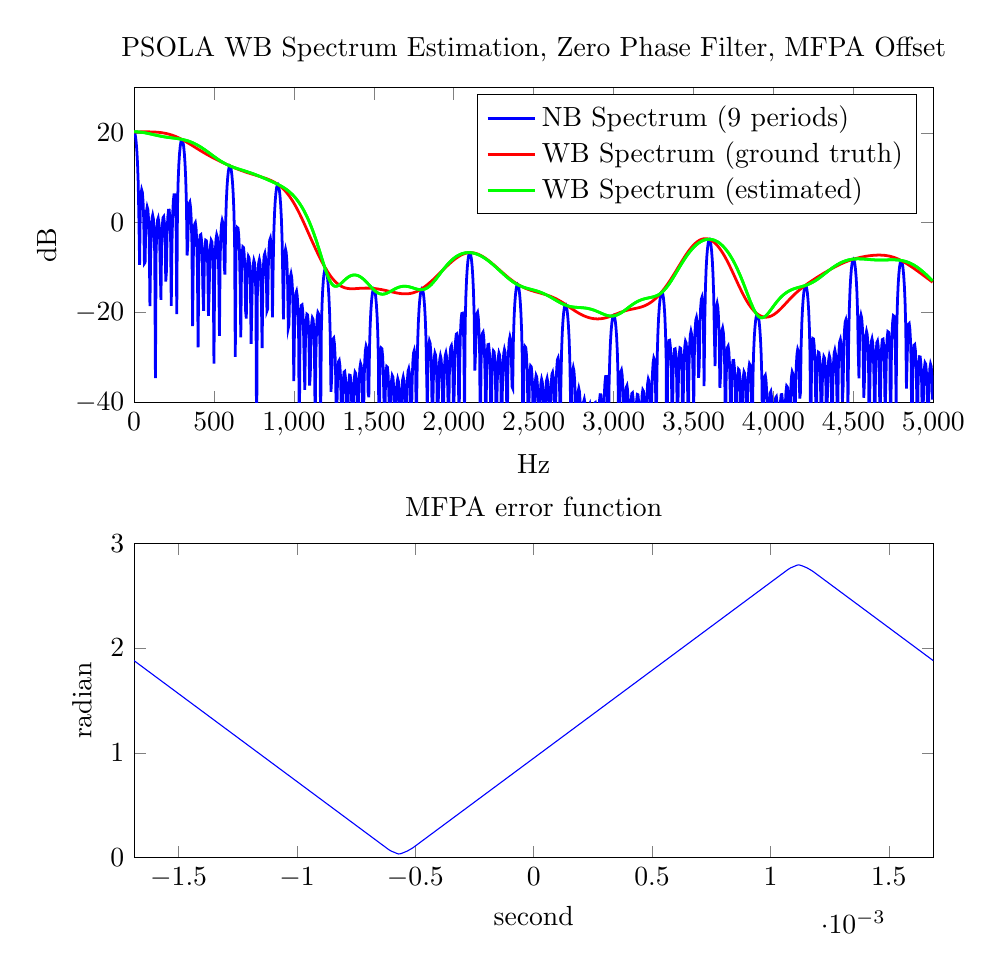
\begin{tikzpicture}

\begin{axis}[%
width=3.996in,
height=1.573in,
at={(0.67in,2.889in)},
scale only axis,
xmin=0,
xmax=5000,
xlabel={Hz},
ymin=-40,
ymax=30,
ylabel={dB},
axis background/.style={fill=white},
title={PSOLA WB Spectrum Estimation, Zero Phase Filter, MFPA Offset},
legend style={legend cell align=left,align=left,legend plot pos=left,draw=black}
]
\addplot [color=blue,solid,line width=1.0pt]
  table[row sep=crcr]{%
0	20.1998112835222\\
4.306640625	19.9630253719877\\
8.61328125	19.23608456754\\
12.919921875	17.9633168511586\\
17.2265625	16.0268836348929\\
21.533203125	13.180537695682\\
25.83984375	8.82254697532815\\
30.146484375	0.700132934977569\\
34.453125	-9.38373032108902\\
38.759765625	2.98659325302194\\
43.06640625	6.33169751815378\\
47.373046875	7.30266916969746\\
51.6796875	6.77667170122703\\
55.986328125	4.80429821792679\\
60.29296875	0.7501749063269\\
64.599609375	-9.06739986575636\\
68.90625	-8.84633817460019\\
73.212890625	-0.448845915708003\\
77.51953125	2.54030046703731\\
81.826171875	3.47160196499781\\
86.1328125	2.92848316932768\\
90.439453125	0.823665138553798\\
94.74609375	-3.79589932080678\\
99.052734375	-18.5756772250071\\
103.359375	-7.93671101154218\\
107.666015625	-1.59488202972874\\
111.97265625	0.938574716105091\\
116.279296875	1.65231291420388\\
120.5859375	0.911077700369427\\
124.892578125	-1.52749595363338\\
129.19921875	-7.11592771881383\\
133.505859375	-34.5722811525766\\
137.8125	-6.61373570433565\\
142.119140625	-1.57112836514892\\
146.42578125	0.545998752837385\\
150.732421875	1.00846814542794\\
155.0390625	0.0075301437058071\\
159.345703125	-2.88396867964477\\
163.65234375	-9.97838652093608\\
167.958984375	-17.192771912636\\
172.265625	-4.78035058609264\\
176.572265625	-0.638400915645049\\
180.87890625	1.12216088386889\\
185.185546875	1.33907394831947\\
189.4921875	0.0523510917985334\\
193.798828125	-3.40616894653223\\
198.10546875	-13.0783608409664\\
202.412109375	-10.8149065958478\\
206.71875	-2.21399372933633\\
211.025390625	1.29323255945514\\
215.33203125	2.78023534109459\\
219.638671875	2.79677847346454\\
223.9453125	1.23710594004096\\
228.251953125	-2.90986290783263\\
232.55859375	-18.5287228243133\\
236.865234375	-5.07437946200522\\
241.171875	1.68146476444492\\
245.478515625	4.82865626022634\\
249.78515625	6.22513811815499\\
254.091796875	6.21700281802173\\
258.3984375	4.54902151417185\\
262.705078125	-0.316094181416908\\
267.01171875	-20.363133887073\\
271.318359375	3.0575328404054\\
275.625	9.27891446263824\\
279.931640625	12.9384014511283\\
284.23828125	15.3605742145365\\
288.544921875	16.976883161126\\
292.8515625	17.977230460254\\
297.158203125	18.4540711714899\\
301.46484375	18.4483724573271\\
305.771484375	17.9654553462524\\
310.078125	16.9768332061207\\
314.384765625	15.4096533081199\\
318.69140625	13.1137631497759\\
322.998046875	9.76421522356001\\
327.3046875	4.48366627441882\\
331.611328125	-7.28779632516265\\
335.91796875	-4.96268448321749\\
340.224609375	1.99861892255419\\
344.53125	4.24016109828536\\
348.837890625	4.56604740982572\\
353.14453125	3.47389497384442\\
357.451171875	0.821822750435316\\
361.7578125	-4.47933965328061\\
366.064453125	-22.9871894100464\\
370.37109375	-7.9276733181233\\
374.677734375	-2.4009082371425\\
378.984375	-0.34229117257703\\
383.291015625	-0.0312866799537609\\
387.59765625	-1.16210097745387\\
391.904296875	-4.0315085335604\\
396.2109375	-10.3064806049518\\
400.517578125	-27.7454714802381\\
404.82421875	-8.96041585014565\\
409.130859375	-4.50057833605844\\
413.4375	-2.76654898886159\\
417.744140625	-2.64331954205402\\
422.05078125	-3.98848856452724\\
426.357421875	-7.29656566264157\\
430.6640625	-15.2784849930523\\
434.970703125	-19.6280355318497\\
439.27734375	-8.99724198244873\\
443.583984375	-5.32514569278338\\
447.890625	-3.90870032064053\\
452.197265625	-4.01131670320744\\
456.50390625	-5.63872421867575\\
460.810546875	-9.55198647649263\\
465.1171875	-20.7180949277035\\
469.423828125	-15.7930572842945\\
473.73046875	-8.16917574371243\\
478.037109375	-5.08890565936573\\
482.34375	-3.95112379091371\\
486.650390625	-4.27886231094048\\
490.95703125	-6.22662529777623\\
495.263671875	-10.9467752816124\\
499.5703125	-31.3720859569978\\
503.876953125	-12.300503406473\\
508.18359375	-6.31416732449098\\
512.490234375	-3.66153423458226\\
516.796875	-2.73342069721742\\
521.103515625	-3.24679885715659\\
525.41015625	-5.52163875890404\\
529.716796875	-11.3416098083815\\
534.0234375	-25.1884258090493\\
538.330078125	-7.88815132235102\\
542.63671875	-2.8370304498133\\
546.943359375	-0.390318856198591\\
551.25	0.506452892803202\\
555.556640625	-0.0166488445335278\\
559.86328125	-2.47547139389485\\
564.169921875	-9.79720288032116\\
568.4765625	-11.5585691503197\\
572.783203125	-0.26091673753151\\
577.08984375	4.80216787241052\\
581.396484375	7.96660497742971\\
585.703125	10.0888750043705\\
590.009765625	11.4884635150531\\
594.31640625	12.3134393672655\\
598.623046875	12.6356428150781\\
602.9296875	12.4829286915673\\
607.236328125	11.8494215428484\\
611.54296875	10.6934381166779\\
615.849609375	8.92126294594062\\
620.15625	6.34018678646955\\
624.462890625	2.51060127598473\\
628.76953125	-3.93058795833235\\
633.076171875	-29.8765932710116\\
637.3828125	-7.22073502622392\\
641.689453125	-2.58802146404613\\
645.99609375	-1.08406020592237\\
650.302734375	-1.22451747362509\\
654.609375	-2.76748022153114\\
658.916015625	-6.07369718453135\\
663.22265625	-13.0703607360523\\
667.529296875	-25.4888922745812\\
671.8359375	-10.7681483752551\\
676.142578125	-6.80085350391991\\
680.44921875	-5.37724987757188\\
684.755859375	-5.51878325723298\\
689.0625	-7.1315311122338\\
693.369140625	-10.7845908709031\\
697.67578125	-19.6906533715383\\
701.982421875	-21.3319460156931\\
706.2890625	-12.0232578629801\\
710.595703125	-8.70507389456911\\
714.90234375	-7.5296288794478\\
719.208984375	-7.85076189366707\\
723.515625	-9.72012955502276\\
727.822265625	-14.0032084210673\\
732.12890625	-26.9681252466484\\
736.435546875	-18.9683562373307\\
740.7421875	-12.0946102853705\\
745.048828125	-9.31566119981948\\
749.35546875	-8.40778528496611\\
753.662109375	-8.96009418001901\\
757.96875	-11.1765644443649\\
762.275390625	-16.3715623363842\\
766.58203125	-50.4097796660791\\
770.888671875	-16.6493913596753\\
775.1953125	-11.2182619719317\\
779.501953125	-8.87541761698952\\
783.80859375	-8.21733972168566\\
788.115234375	-9.01484960341191\\
792.421875	-11.648075063922\\
796.728515625	-18.1820357938765\\
801.03515625	-27.8814775292402\\
805.341796875	-13.7899469385954\\
809.6484375	-9.2977812257912\\
813.955078125	-7.28269888018684\\
818.26171875	-6.82222429053385\\
822.568359375	-7.84092832395503\\
826.875	-10.9426852950643\\
831.181640625	-19.6363166678899\\
835.48828125	-19.2147063656537\\
839.794921875	-9.70840578203416\\
844.1015625	-5.77335054614669\\
848.408203125	-3.89682500612588\\
852.71484375	-3.46440743891657\\
857.021484375	-4.53847095401937\\
861.328125	-8.0257594005086\\
865.634765625	-21.0448351144762\\
869.94140625	-10.0975033682217\\
874.248046875	-2.19570974801476\\
878.5546875	2.03661450733223\\
882.861328125	4.77327991030721\\
887.16796875	6.6032194301663\\
891.474609375	7.76851034651357\\
895.78125	8.38503996787751\\
900.087890625	8.50728034555433\\
904.39453125	8.15087262548289\\
908.701171875	7.29829713514368\\
913.0078125	5.89269631782302\\
917.314453125	3.81429563711903\\
921.62109375	0.812656854290675\\
925.927734375	-3.72703921020973\\
930.234375	-12.1406567418575\\
934.541015625	-21.4830202864805\\
938.84765625	-9.79457197744449\\
943.154296875	-6.68408878585383\\
947.4609375	-5.91921294684327\\
951.767578125	-6.65127720994375\\
956.07421875	-8.84128054323327\\
960.380859375	-13.1459570571033\\
964.6875	-23.4280442743385\\
968.994140625	-22.709719872331\\
973.30078125	-14.7526538181588\\
977.607421875	-12.0393862707918\\
981.9140625	-11.367405002163\\
986.220703125	-12.1729641316058\\
990.52734375	-14.554974476215\\
994.833984375	-19.497806500199\\
999.140625	-35.2394591524033\\
1003.447265625	-23.7992484742012\\
1007.75390625	-17.8583217243373\\
1012.060546875	-15.6433421617602\\
1016.3671875	-15.2379996403687\\
1020.673828125	-16.2922566678487\\
1024.98046875	-19.0614117755215\\
1029.287109375	-25.0486156600312\\
1033.59375	-49.0489298744527\\
1037.900390625	-24.8089474791962\\
1042.20703125	-20.1642051629567\\
1046.513671875	-18.3959969215619\\
1050.8203125	-18.27482670725\\
1055.126953125	-19.6214733178922\\
1059.43359375	-22.8791216784764\\
1063.740234375	-30.453023958123\\
1068.046875	-37.1668259432527\\
1072.353515625	-25.5193464844901\\
1076.66015625	-21.7657194537968\\
1080.966796875	-20.3597753890085\\
1085.2734375	-20.4900968934607\\
1089.580078125	-22.1277479504058\\
1093.88671875	-25.9629878121736\\
1098.193359375	-36.246288353504\\
1102.5	-33.579046995292\\
1106.806640625	-25.4932405938991\\
1111.11328125	-22.3449582762696\\
1115.419921875	-21.1911183365883\\
1119.7265625	-21.5004356503055\\
1124.033203125	-23.3902135871153\\
1128.33984375	-27.9048834166156\\
1132.646484375	-44.71021669476\\
1136.953125	-30.2833735281743\\
1141.259765625	-23.9262840157376\\
1145.56640625	-21.0912990386407\\
1149.873046875	-19.9863477151915\\
1154.1796875	-20.2795711245027\\
1158.486328125	-22.2395360091323\\
1162.79296875	-27.4586537681424\\
1167.099609375	-45.5842703043268\\
1171.40625	-24.208913962963\\
1175.712890625	-18.2949447075252\\
1180.01953125	-14.8851474285416\\
1184.326171875	-12.691793179793\\
1188.6328125	-11.2912663526898\\
1192.939453125	-10.4963235453979\\
1197.24609375	-10.2156758905104\\
1201.552734375	-10.409005429178\\
1205.859375	-11.0714974932496\\
1210.166015625	-12.2322401946023\\
1214.47265625	-13.9650917440467\\
1218.779296875	-16.4223228607886\\
1223.0859375	-19.9344895079399\\
1227.392578125	-25.4005568635528\\
1231.69921875	-37.623188516167\\
1236.005859375	-34.6680758793\\
1240.3125	-27.9948271285995\\
1244.619140625	-25.8959847463931\\
1248.92578125	-25.683528706939\\
1253.232421875	-26.8777750985092\\
1257.5390625	-29.6326465032016\\
1261.845703125	-35.0734378595294\\
1266.15234375	-54.8514111494645\\
1270.458984375	-38.2663073589711\\
1274.765625	-32.8892446605226\\
1279.072265625	-30.8979209049996\\
1283.37890625	-30.6323428303362\\
1287.685546875	-31.8008951825488\\
1291.9921875	-34.7145473825549\\
1296.298828125	-41.1009414379874\\
1300.60546875	-56.9684303751582\\
1304.912109375	-39.3767095308271\\
1309.21875	-34.9724418251893\\
1313.525390625	-33.2423355395328\\
1317.83203125	-33.1077033036382\\
1322.138671875	-34.4384819187939\\
1326.4453125	-37.7474861954958\\
1330.751953125	-45.8624091037353\\
1335.05859375	-49.4140706504964\\
1339.365234375	-39.0528148799068\\
1343.671875	-35.3738455545236\\
1347.978515625	-33.9175179842497\\
1352.28515625	-33.9714243243948\\
1356.591796875	-35.5531776289138\\
1360.8984375	-39.4494845609004\\
1365.205078125	-50.9154468913804\\
1369.51171875	-45.1326178453323\\
1373.818359375	-37.5949115093331\\
1378.125	-34.4764153065035\\
1382.431640625	-33.2801282349985\\
1386.73828125	-33.5465859458439\\
1391.044921875	-35.4428279490626\\
1395.3515625	-40.1602903228542\\
1399.658203125	-62.3297224810393\\
1403.96484375	-40.9954754608816\\
1408.271484375	-35.0323131589968\\
1412.578125	-32.335428741381\\
1416.884765625	-31.3511414856145\\
1421.19140625	-31.8101434649748\\
1425.498046875	-34.0469706380057\\
1429.8046875	-39.9115513397173\\
1434.111328125	-52.432203015717\\
1438.41796875	-35.9521334061734\\
1442.724609375	-30.9035515648031\\
1447.03125	-28.4186983429005\\
1451.337890625	-27.4766663741978\\
1455.64453125	-27.9592071848347\\
1459.951171875	-30.400945804758\\
1464.2578125	-37.8600226117026\\
1468.564453125	-38.8379654253097\\
1472.87109375	-27.7691133825669\\
1477.177734375	-22.69927135973\\
1481.484375	-19.4999703896788\\
1485.791015625	-17.3350331009931\\
1490.09765625	-15.890432924203\\
1494.404296875	-15.0202668600617\\
1498.7109375	-14.6538135445525\\
1503.017578125	-14.7639690911613\\
1507.32421875	-15.3572926702582\\
1511.630859375	-16.4763221183481\\
1515.9375	-18.2161828743193\\
1520.244140625	-20.7725697301831\\
1524.55078125	-24.5935722313346\\
1528.857421875	-31.0824962855242\\
1533.1640625	-60.4598530224238\\
1537.470703125	-33.9555297758027\\
1541.77734375	-29.3920971204874\\
1546.083984375	-27.8964812898769\\
1550.390625	-28.035072508889\\
1554.697265625	-29.579050308284\\
1559.00390625	-32.9040286199559\\
1563.310546875	-40.0097976136181\\
1567.6171875	-51.3458087865995\\
1571.923828125	-37.3078224679822\\
1576.23046875	-33.3955416719199\\
1580.537109375	-31.9889196327076\\
1584.84375	-32.1406755961283\\
1589.150390625	-33.7684818610118\\
1593.45703125	-37.461074618364\\
1597.763671875	-46.5794090591401\\
1602.0703125	-47.5026971254225\\
1606.376953125	-38.444684234083\\
1610.68359375	-35.1711542587568\\
1614.990234375	-34.0147420882645\\
1619.296875	-34.3504536543766\\
1623.603515625	-36.2413636456998\\
1627.91015625	-40.5813122809749\\
1632.216796875	-54.0586748113481\\
1636.5234375	-45.1511662193199\\
1640.830078125	-38.4103549697745\\
1645.13671875	-35.6619163960994\\
1649.443359375	-34.7659671209367\\
1653.75	-35.3272568819416\\
1658.056640625	-37.5623193933281\\
1662.36328125	-42.8305022656014\\
1666.669921875	-104.975627864264\\
1670.9765625	-42.717604695922\\
1675.283203125	-37.3553873885377\\
1679.58984375	-35.0202604587396\\
1683.896484375	-34.3553802702821\\
1688.203125	-35.144232930603\\
1692.509765625	-37.7822635581355\\
1696.81640625	-44.4144134074196\\
1701.123046875	-53.1280943956726\\
1705.4296875	-39.5573704178631\\
1709.736328125	-35.07949289342\\
1714.04296875	-33.0373626179028\\
1718.349609375	-32.5376620408381\\
1722.65625	-33.5163269255627\\
1726.962890625	-36.5977760741338\\
1731.26953125	-45.4598132167914\\
1735.576171875	-44.2477307582468\\
1739.8828125	-34.8845286516843\\
1744.189453125	-30.9041931763623\\
1748.49609375	-28.9514924848564\\
1752.802734375	-28.4319819416156\\
1757.109375	-29.4194219138004\\
1761.416015625	-32.8506836319926\\
1765.72265625	-46.3693479059954\\
1770.029296875	-34.2808675853555\\
1774.3359375	-26.3628331147012\\
1778.642578125	-22.0122308433041\\
1782.94921875	-19.129899122797\\
1787.255859375	-17.1389723439664\\
1791.5625	-15.8010945562484\\
1795.869140625	-15.0019390297895\\
1800.17578125	-14.6878616987227\\
1804.482421875	-14.8438022918568\\
1808.7890625	-15.4878698935034\\
1813.095703125	-16.6777839253265\\
1817.40234375	-18.5349729913049\\
1821.708984375	-21.3138736996628\\
1826.015625	-25.6425350556161\\
1830.322265625	-33.9442357631557\\
1834.62890625	-42.159778828701\\
1838.935546875	-30.6691299334826\\
1843.2421875	-27.3357991244035\\
1847.548828125	-26.3048246789006\\
1851.85546875	-26.7550654832247\\
1856.162109375	-28.6590233318075\\
1860.46875	-32.6953489773781\\
1864.775390625	-42.9213436578096\\
1869.08203125	-41.1489376371587\\
1873.388671875	-33.0534286338037\\
1877.6953125	-30.0312833856612\\
1882.001953125	-29.0189621057011\\
1886.30859375	-29.472139191443\\
1890.615234375	-31.5016981963111\\
1894.921875	-36.1247461605528\\
1899.228515625	-52.2578403012026\\
1903.53515625	-39.2574248082269\\
1907.841796875	-33.0260177179211\\
1912.1484375	-30.4289537567346\\
1916.455078125	-29.6194221961028\\
1920.76171875	-30.2624592705681\\
1925.068359375	-32.6271739562901\\
1929.375	-38.2703138400956\\
1933.681640625	-59.1053107170634\\
1937.98828125	-36.7723546280088\\
1942.294921875	-31.7508965230763\\
1946.6015625	-29.5519941440276\\
1950.908203125	-28.9868629796253\\
1955.21484375	-29.8891754300279\\
1959.521484375	-32.7195201566249\\
1963.828125	-39.9823037777115\\
1968.134765625	-45.4239486243501\\
1972.44140625	-33.7083673055819\\
1976.748046875	-29.5421161838923\\
1981.0546875	-27.6922591596885\\
1985.361328125	-27.3739259187386\\
1989.66796875	-28.5702486797767\\
1993.974609375	-31.9952070412372\\
1998.28125	-42.1255400890556\\
2002.587890625	-38.2680387530637\\
2006.89453125	-29.91853024375\\
2011.201171875	-26.3667640788614\\
2015.5078125	-24.7931542177167\\
2019.814453125	-24.6852613778683\\
2024.12109375	-26.1727921058266\\
2028.427734375	-30.3354667333159\\
2032.734375	-47.7581888101633\\
2037.041015625	-31.5232002614905\\
2041.34765625	-24.876449407978\\
2045.654296875	-21.6822384967924\\
2049.9609375	-20.2118945880203\\
2054.267578125	-20.1480784260864\\
2058.57421875	-21.7734430864586\\
2062.880859375	-26.7385858397401\\
2067.1875	-42.708700428162\\
2071.494140625	-22.4378333488712\\
2075.80078125	-16.2683508974895\\
2080.107421875	-12.5651381215624\\
2084.4140625	-10.0764462050578\\
2088.720703125	-8.38683419825366\\
2093.02734375	-7.31216788454593\\
2097.333984375	-6.76277219545392\\
2101.640625	-6.69940156077409\\
2105.947265625	-7.11813982451677\\
2110.25390625	-8.04903307402283\\
2114.560546875	-9.56726258570305\\
2118.8671875	-11.8275029770146\\
2123.173828125	-15.1662350396393\\
2127.48046875	-20.5049146020514\\
2131.787109375	-32.9100769045871\\
2136.09375	-29.0395765996548\\
2140.400390625	-22.3989819647033\\
2144.70703125	-20.2167909234129\\
2149.013671875	-19.9144179059004\\
2153.3203125	-21.0295818274495\\
2157.626953125	-23.7281899198547\\
2161.93359375	-29.1728114028156\\
2166.240234375	-50.3589251886418\\
2170.546875	-31.9000225432334\\
2174.853515625	-26.5942818768441\\
2179.16015625	-24.6152600519339\\
2183.466796875	-24.360431472575\\
2187.7734375	-25.5516848828998\\
2192.080078125	-28.5139334409282\\
2196.38671875	-35.0378142404274\\
2200.693359375	-49.5540306033278\\
2205	-33.0309661651897\\
2209.306640625	-28.7545863346986\\
2213.61328125	-27.1184432211859\\
2217.919921875	-27.0782027772328\\
2222.2265625	-28.5153067616549\\
2226.533203125	-31.9605165299862\\
2230.83984375	-40.364608386995\\
2235.146484375	-43.290638500833\\
2239.453125	-33.3493502412746\\
2243.759765625	-29.8439703942752\\
2248.06640625	-28.5387674596199\\
2252.373046875	-28.7439303790343\\
2256.6796875	-30.4880411514058\\
2260.986328125	-34.5832900040212\\
2265.29296875	-46.5990079962944\\
2269.599609375	-40.1606411578983\\
2273.90625	-32.9316144331267\\
2278.212890625	-30.0067619638697\\
2282.51953125	-28.9867621626858\\
2286.826171875	-29.4284899008207\\
2291.1328125	-31.5108882684296\\
2295.439453125	-36.4652575902806\\
2299.74609375	-61.2066612643271\\
2304.052734375	-37.2553728178305\\
2308.359375	-31.5458692506253\\
2312.666015625	-29.035640274934\\
2316.97265625	-28.2236854712399\\
2321.279296875	-28.8538055464397\\
2325.5859375	-31.2750064812107\\
2329.892578125	-37.4064038219762\\
2334.19921875	-48.9209127322706\\
2338.505859375	-33.3616908672706\\
2342.8125	-28.5190632759566\\
2347.119140625	-26.1964438496571\\
2351.42578125	-25.4052179629118\\
2355.732421875	-26.0387481154547\\
2360.0390625	-28.6507532732254\\
2364.345703125	-36.4386213527499\\
2368.65234375	-36.8163491943689\\
2372.958984375	-26.1301138650274\\
2377.265625	-21.2175385284303\\
2381.572265625	-18.1425396639748\\
2385.87890625	-16.0884906929407\\
2390.185546875	-14.7466392148609\\
2394.4921875	-13.9731744163814\\
2398.798828125	-13.6984615603574\\
2403.10546875	-13.8961349375531\\
2407.412109375	-14.5734344582199\\
2411.71875	-15.7737572192914\\
2416.025390625	-17.5936582548208\\
2420.33203125	-20.231881585671\\
2424.638671875	-24.1452395670679\\
2428.9453125	-30.7789884808892\\
2433.251953125	-66.4019714005567\\
2437.55859375	-33.4074703280699\\
2441.865234375	-28.9879567938483\\
2446.171875	-27.5724003695478\\
2450.478515625	-27.7760131848556\\
2454.78515625	-29.3830933938643\\
2459.091796875	-32.7846167155161\\
2463.3984375	-40.0568703455795\\
2467.705078125	-50.4272523462117\\
2472.01171875	-37.0441199644354\\
2476.318359375	-33.2257025076207\\
2480.625	-31.8728526751233\\
2484.931640625	-32.0688715430471\\
2489.23828125	-33.7433300913393\\
2493.544921875	-37.5054852884543\\
2497.8515625	-46.8750563107116\\
2502.158203125	-47.1081286610323\\
2506.46484375	-38.3111364715555\\
2510.771484375	-35.1047625605345\\
2515.078125	-33.9902625189903\\
2519.384765625	-34.3636517375759\\
2523.69140625	-36.2998843853299\\
2527.998046875	-40.7225440491012\\
2532.3046875	-54.7896197419302\\
2536.611328125	-44.9542821464144\\
2540.91796875	-38.3705088203464\\
2545.224609375	-35.6840366812206\\
2549.53125	-34.8350944353936\\
2553.837890625	-35.4442157816235\\
2558.14453125	-37.7411012345374\\
2562.451171875	-43.1324081573405\\
2566.7578125	-76.1903702669056\\
2571.064453125	-42.7385762421682\\
2575.37109375	-37.5061264459909\\
2579.677734375	-35.2482265105403\\
2583.984375	-34.6533440754984\\
2588.291015625	-35.5179594218759\\
2592.59765625	-38.2536115489535\\
2596.904296875	-45.089822664367\\
2601.2109375	-52.9737115194338\\
2605.517578125	-39.9911606084764\\
2609.82421875	-35.6541256906912\\
2614.130859375	-33.7228274927983\\
2618.4375	-33.332607844849\\
2622.744140625	-34.4311624454065\\
2627.05078125	-37.6644405259101\\
2631.357421875	-46.8918910900143\\
2635.6640625	-45.0820072585853\\
2639.970703125	-36.0577556410085\\
2644.27734375	-32.251657772857\\
2648.583984375	-30.456208457312\\
2652.890625	-30.0967052027532\\
2657.197265625	-31.2586045241921\\
2661.50390625	-34.9101682939826\\
2665.810546875	-49.2903375582174\\
2670.1171875	-36.2939839737482\\
2674.423828125	-28.6721711416799\\
2678.73046875	-24.5341803089396\\
2683.037109375	-21.8517763252526\\
2687.34375	-20.059705261204\\
2691.650390625	-18.9230923415622\\
2695.95703125	-18.3289488428089\\
2700.263671875	-18.2242316347043\\
2704.5703125	-18.5942320146949\\
2708.876953125	-19.4574213226666\\
2713.18359375	-20.8721590766889\\
2717.490234375	-22.9613185247052\\
2721.796875	-25.9831738762416\\
2726.103515625	-30.5791396542569\\
2730.41015625	-39.2645072078657\\
2734.716796875	-46.8868912081726\\
2739.0234375	-36.0683847592672\\
2743.330078125	-33.033998291045\\
2747.63671875	-32.2705057676124\\
2751.943359375	-32.9831354304212\\
2756.25	-35.1555622573567\\
2760.556640625	-39.4886625892801\\
2764.86328125	-50.2490263184005\\
2769.169921875	-47.9978043651481\\
2773.4765625	-40.3451170198691\\
2777.783203125	-37.6128311072675\\
2782.08984375	-36.8675733970998\\
2786.396484375	-37.5835530927324\\
2790.703125	-39.8832628647441\\
2795.009765625	-44.8172457163679\\
2799.31640625	-62.0877268366828\\
2803.623046875	-48.0597959551908\\
2807.9296875	-42.1796220536976\\
2812.236328125	-39.8505110391258\\
2816.54296875	-39.2914002758121\\
2820.849609375	-40.181558693505\\
2825.15625	-42.8034805108976\\
2829.462890625	-48.7692135109422\\
2833.76953125	-67.6710054338781\\
2838.076171875	-47.3425449887743\\
2842.3828125	-42.6081152478516\\
2846.689453125	-40.6435311360391\\
2850.99609375	-40.2984899861726\\
2855.302734375	-41.4186885424439\\
2859.609375	-44.4817230498859\\
2863.916015625	-52.0960084439547\\
2868.22265625	-56.939567412072\\
2872.529296875	-45.7727364846558\\
2876.8359375	-41.8325485327789\\
2881.142578125	-40.1717129254251\\
2885.44921875	-40.0303520492362\\
2889.755859375	-41.4028996513451\\
2894.0625	-45.0270028655651\\
2898.369140625	-55.6237214204411\\
2902.67578125	-51.1512675551712\\
2906.982421875	-43.1063760829891\\
2911.2890625	-39.7154463946734\\
2915.595703125	-38.2746563359567\\
2919.90234375	-38.2893687950603\\
2924.208984375	-39.9011849227772\\
2928.515625	-44.2258187205749\\
2932.822265625	-62.9494636879658\\
2937.12890625	-45.2041798725932\\
2941.435546875	-38.7302876848822\\
2945.7421875	-35.6264951426347\\
2950.048828125	-34.224306295174\\
2954.35546875	-34.2202822252036\\
2958.662109375	-35.9110012387153\\
2962.96875	-41.0075372856128\\
2967.275390625	-55.432099012491\\
2971.58203125	-36.3630249381074\\
2975.888671875	-30.2626854342915\\
2980.1953125	-26.5734882908228\\
2984.501953125	-24.0781107449736\\
2988.80859375	-22.3689666902281\\
2993.115234375	-21.2649081185317\\
2997.421875	-20.6778328029487\\
3001.728515625	-20.5695797990146\\
3006.03515625	-20.937185179566\\
3010.341796875	-21.8117440983916\\
3014.6484375	-23.269892623203\\
3018.955078125	-25.4688987841688\\
3023.26171875	-28.7514891328905\\
3027.568359375	-34.0626142620684\\
3031.875	-46.7568019959351\\
3036.181640625	-42.0140647141124\\
3040.48828125	-35.443524439949\\
3044.794921875	-33.2047677919449\\
3049.1015625	-32.822922223742\\
3053.408203125	-33.8530470795228\\
3057.71484375	-36.4734686098062\\
3062.021484375	-41.8857807126748\\
3066.328125	-64.8001516016807\\
3070.634765625	-44.025663796996\\
3074.94140625	-38.7036824620523\\
3079.248046875	-36.6377587337947\\
3083.5546875	-36.2807264391008\\
3087.861328125	-37.3681478818358\\
3092.16796875	-40.2394882985632\\
3096.474609375	-46.7517506285891\\
3100.78125	-59.8863713418095\\
3105.087890625	-44.1157044402721\\
3109.39453125	-39.7750534340044\\
3113.701171875	-38.030572244552\\
3118.0078125	-37.8714396509153\\
3122.314453125	-39.1908994264135\\
3126.62109375	-42.5384945837206\\
3130.927734375	-50.9962573805875\\
3135.234375	-53.0517202165262\\
3139.541015625	-43.2478594358915\\
3143.84765625	-39.642074274551\\
3148.154296875	-38.2063635805174\\
3152.4609375	-38.2732810474188\\
3156.767578125	-39.8828173386885\\
3161.07421875	-43.8738944616134\\
3165.380859375	-56.1615792805697\\
3169.6875	-48.7221318923853\\
3173.994140625	-41.4716091615697\\
3178.30078125	-38.4104768606487\\
3182.607421875	-37.2323281507421\\
3186.9140625	-37.5104322603686\\
3191.220703125	-39.4361541197169\\
3195.52734375	-44.2826170514028\\
3199.833984375	-72.3506432394789\\
3204.140625	-44.3239096764499\\
3208.447265625	-38.508211668137\\
3212.75390625	-35.8248762739799\\
3217.060546875	-34.8236950404711\\
3221.3671875	-35.2616908725877\\
3225.673828125	-37.5028804501334\\
3229.98046875	-43.5392487927682\\
3234.287109375	-53.764372522248\\
3238.59375	-38.6701079460653\\
3242.900390625	-33.6625265477598\\
3247.20703125	-31.132117606795\\
3251.513671875	-30.1216839461902\\
3255.8203125	-30.5363610541038\\
3260.126953125	-32.9496911837841\\
3264.43359375	-40.7078187367719\\
3268.740234375	-40.1211162254614\\
3273.046875	-29.4343011190198\\
3277.353515625	-24.3111945823205\\
3281.66015625	-20.9948692531592\\
3285.966796875	-18.6878065331956\\
3290.2734375	-17.0865701493412\\
3294.580078125	-16.0495393873017\\
3298.88671875	-15.5082634638675\\
3303.193359375	-15.4372026039188\\
3307.5	-15.8443564355347\\
3311.806640625	-16.7740550210522\\
3316.11328125	-18.3243586101523\\
3320.419921875	-20.6971624425378\\
3324.7265625	-24.3582605941697\\
3329.033203125	-30.7966691829404\\
3333.33984375	-87.8983120796898\\
3337.646484375	-32.5023850324611\\
3341.953125	-27.8882018952338\\
3346.259765625	-26.2187379287321\\
3350.56640625	-26.1560245525743\\
3354.873046875	-27.4972698165486\\
3359.1796875	-30.6490528995852\\
3363.486328125	-37.7680263934394\\
3367.79296875	-46.906092879075\\
3372.099609375	-33.7968194323486\\
3376.40625	-29.7516210802337\\
3380.712890625	-28.1349599333455\\
3385.01953125	-28.0596478268375\\
3389.326171875	-29.4670270537715\\
3393.6328125	-32.9873452383092\\
3397.939453125	-42.3101776905498\\
3402.24609375	-41.5434651589063\\
3406.552734375	-32.6866986969943\\
3410.859375	-29.2399202480361\\
3415.166015625	-27.8619795369593\\
3419.47265625	-27.9693693184201\\
3423.779296875	-29.6489764186699\\
3428.0859375	-33.8551232256215\\
3432.392578125	-48.2737949775696\\
3436.69921875	-37.1552826576038\\
3441.005859375	-30.42698188668\\
3445.3125	-27.5067787922715\\
3449.619140625	-26.4111308502796\\
3453.92578125	-26.7760756103137\\
3458.232421875	-28.8446508639845\\
3462.5390625	-34.0727967882197\\
3466.845703125	-60.8312370801053\\
3471.15234375	-32.8238839446013\\
3475.458984375	-27.4338479325378\\
3479.765625	-24.9692983488222\\
3484.072265625	-24.1622081578445\\
3488.37890625	-24.8218552108221\\
3492.685546875	-27.3761433023414\\
3496.9921875	-34.143643794238\\
3501.298828125	-40.9591755531387\\
3505.60546875	-28.244746040393\\
3509.912109375	-23.7716761263397\\
3514.21875	-21.6764454204785\\
3518.525390625	-21.1220995217472\\
3522.83203125	-22.0680023634783\\
3527.138671875	-25.1821719476247\\
3531.4453125	-34.5192444999425\\
3535.751953125	-31.8361398390348\\
3540.05859375	-22.8701361979892\\
3544.365234375	-18.9681772198909\\
3548.671875	-17.0613482188096\\
3552.978515625	-16.5942517106421\\
3557.28515625	-17.6641785007549\\
3561.591796875	-21.2719771192209\\
3565.8984375	-36.3384384223703\\
3570.205078125	-22.0843764093747\\
3574.51171875	-14.4923292148138\\
3578.818359375	-10.3061564191412\\
3583.125	-7.56547198978778\\
3587.431640625	-5.71671355213846\\
3591.73828125	-4.52887142425399\\
3596.044921875	-3.8907679403945\\
3600.3515625	-3.75047448257036\\
3604.658203125	-4.0941657411104\\
3608.96484375	-4.94121170103912\\
3613.271484375	-6.35114622091155\\
3617.578125	-8.44882395653159\\
3621.884765625	-11.4969361550655\\
3626.19140625	-16.1511484125964\\
3630.498046875	-25.0244773201722\\
3634.8046875	-31.8867060021555\\
3639.111328125	-21.5214674090735\\
3643.41796875	-18.6076776586481\\
3647.724609375	-17.9436676438842\\
3652.03125	-18.7606059677341\\
3656.337890625	-21.0536836934662\\
3660.64453125	-25.5469853120076\\
3664.951171875	-36.7334937278781\\
3669.2578125	-33.8773785700906\\
3673.564453125	-26.5533106808914\\
3677.87109375	-24.0164771243579\\
3682.177734375	-23.4561643115808\\
3686.484375	-24.3648384373626\\
3690.791015625	-26.8768177748531\\
3695.09765625	-32.0773938550946\\
3699.404296875	-50.5931719071312\\
3703.7109375	-35.375970378973\\
3708.017578125	-29.8329631278204\\
3712.32421875	-27.773163423102\\
3716.630859375	-27.4781507221329\\
3720.9375	-28.641032825059\\
3725.244140625	-31.5577057211767\\
3729.55078125	-37.8977978395739\\
3733.857421875	-55.2812537815576\\
3738.1640625	-36.6704049518938\\
3742.470703125	-32.301449698233\\
3746.77734375	-30.6615062142649\\
3751.083984375	-30.636984189085\\
3755.390625	-32.0851176598328\\
3759.697265625	-35.5005039421424\\
3764.00390625	-43.601261011313\\
3768.310546875	-48.0012627869981\\
3772.6171875	-37.5008205598255\\
3776.923828125	-33.9362508269092\\
3781.23046875	-32.6220176789301\\
3785.537109375	-32.822129963373\\
3789.84375	-34.5419603726995\\
3794.150390625	-38.5431786203963\\
3798.45703125	-49.8119546447337\\
3802.763671875	-44.8962254177838\\
3807.0703125	-37.3404279095748\\
3811.376953125	-34.3065508952583\\
3815.68359375	-33.1996899809383\\
3819.990234375	-33.542313768657\\
3824.296875	-35.4877487795748\\
3828.603515625	-40.1888028734443\\
3832.91015625	-60.6868533208456\\
3837.216796875	-41.3937950472722\\
3841.5234375	-35.310552144125\\
3845.830078125	-32.5206178059642\\
3850.13671875	-31.4128225007899\\
3854.443359375	-31.697193864393\\
3858.75	-33.6842372370628\\
3863.056640625	-39.148092587253\\
3867.36328125	-52.4386785617657\\
3871.669921875	-34.6258205302705\\
3875.9765625	-28.8280826027843\\
3880.283203125	-25.3883706375989\\
3884.58984375	-23.1220755311607\\
3888.896484375	-21.6288240655797\\
3893.203125	-20.7299114842943\\
3897.509765625	-20.33826943484\\
3901.81640625	-20.4162778600684\\
3906.123046875	-20.9613835418262\\
3910.4296875	-22.0052013528204\\
3914.736328125	-23.6253160396497\\
3919.04296875	-25.9811257412618\\
3923.349609375	-29.4212572468445\\
3927.65625	-34.9145077763415\\
3931.962890625	-48.1301612612394\\
3936.26953125	-42.6888136089186\\
3940.576171875	-36.3720288025238\\
3944.8828125	-34.2599103159101\\
3949.189453125	-33.9753732881673\\
3953.49609375	-35.0901511333491\\
3957.802734375	-37.7948561348005\\
3962.109375	-43.3314065871638\\
3966.416015625	-68.7233969112789\\
3970.72265625	-45.1698802974334\\
3975.029296875	-39.9587328910789\\
3979.3359375	-37.9276998052508\\
3983.642578125	-37.5827082075014\\
3987.94921875	-38.6729294850311\\
3992.255859375	-41.5528255813442\\
3996.5625	-48.1492383436923\\
4000.869140625	-60.0919126609132\\
4005.17578125	-45.0433671452409\\
4009.482421875	-40.7081872670854\\
4013.7890625	-38.9208851321676\\
4018.095703125	-38.7035894360785\\
4022.40234375	-39.9619110916289\\
4026.708984375	-43.265330991318\\
4031.015625	-51.8363602786008\\
4035.322265625	-53.0754684195451\\
4039.62890625	-43.4379720972936\\
4043.935546875	-39.775819893374\\
4048.2421875	-38.2547323736206\\
4052.548828125	-38.2298803697086\\
4056.85546875	-39.7535570202294\\
4061.162109375	-43.6931316899987\\
4065.46875	-56.3461948915308\\
4069.775390625	-47.9316970843081\\
4074.08203125	-40.7181718661487\\
4078.388671875	-37.5905901135875\\
4082.6953125	-36.3313370157983\\
4087.001953125	-36.5303845266045\\
4091.30859375	-38.3922550156488\\
4095.615234375	-43.2341217781244\\
4099.921875	-77.591912811047\\
4104.228515625	-42.7562061577272\\
4108.53515625	-36.9604427584962\\
4112.841796875	-34.2427988599219\\
4117.1484375	-33.2020837149911\\
4121.455078125	-33.6086135289248\\
4125.76171875	-35.8418785948113\\
4130.068359375	-41.9705282837634\\
4134.375	-51.1679810891721\\
4138.681640625	-36.6717746606065\\
4142.98828125	-31.7133925625705\\
4147.294921875	-29.2016741106109\\
4151.6015625	-28.2096743425889\\
4155.908203125	-28.6540830580974\\
4160.21484375	-31.1285905612773\\
4164.521484375	-39.1380496895904\\
4168.828125	-37.8683341932206\\
4173.134765625	-27.4560803724333\\
4177.44140625	-22.4200931090986\\
4181.748046875	-19.170211512626\\
4186.0546875	-16.927170130134\\
4190.361328125	-15.3924835160499\\
4194.66796875	-14.4264368866196\\
4198.974609375	-13.9615033212945\\
4203.28125	-13.9727202837412\\
4207.587890625	-14.4686063857182\\
4211.89453125	-15.4941919191477\\
4216.201171875	-17.1488228079065\\
4220.5078125	-19.6373635981454\\
4224.814453125	-23.4345817173337\\
4229.12109375	-30.0749014726437\\
4233.427734375	-63.8869455713352\\
4237.734375	-31.6658402333027\\
4242.041015625	-27.2672532852973\\
4246.34765625	-25.7619786837251\\
4250.654296875	-25.8567335411435\\
4254.9609375	-27.3611900995963\\
4259.267578125	-30.6975325089786\\
4263.57421875	-38.1066714040916\\
4267.880859375	-46.5009224832474\\
4272.1875	-34.0605288150277\\
4276.494140625	-30.2361301543497\\
4280.80078125	-28.8073968000046\\
4285.107421875	-28.9152914713248\\
4289.4140625	-30.5124418831174\\
4293.720703125	-34.2501795301851\\
4298.02734375	-43.9997445299946\\
4302.333984375	-42.6906395799849\\
4306.640625	-34.22229218336\\
4310.947265625	-30.9935265414341\\
4315.25390625	-29.8101658283264\\
4319.560546875	-30.1080504676863\\
4323.8671875	-31.9854210681559\\
4328.173828125	-36.4277324462624\\
4332.48046875	-51.7189841673463\\
4336.787109375	-39.6899776435854\\
4341.09375	-33.250224674879\\
4345.400390625	-30.5277726848316\\
4349.70703125	-29.6110081010706\\
4354.013671875	-30.1505390699836\\
4358.3203125	-32.4022726606907\\
4362.626953125	-37.8729024952794\\
4366.93359375	-61.1166994533236\\
4371.240234375	-36.5463173265365\\
4375.546875	-31.3704581204995\\
4379.853515625	-29.0624592127922\\
4384.16015625	-28.395640505383\\
4388.466796875	-29.1914688320364\\
4392.7734375	-31.8941022845486\\
4397.080078125	-38.9156019833431\\
4401.38671875	-44.9989527671641\\
4405.693359375	-32.805456433112\\
4410	-28.4719038293443\\
4414.306640625	-26.47554417908\\
4418.61328125	-26.0059715563696\\
4422.919921875	-27.0339122116638\\
4427.2265625	-30.2498122151563\\
4431.533203125	-39.9183592536617\\
4435.83984375	-36.5442599049321\\
4440.146484375	-27.8007317805851\\
4444.453125	-23.9606455219489\\
4448.759765625	-22.0851183633019\\
4453.06640625	-21.6374234973322\\
4457.373046875	-22.7265986475699\\
4461.6796875	-26.3870773194769\\
4465.986328125	-42.329885031002\\
4470.29296875	-26.7707134984269\\
4474.599609375	-19.2491329329316\\
4478.90625	-15.0422376130894\\
4483.212890625	-12.254106531457\\
4487.51953125	-10.3423651644057\\
4491.826171875	-9.07959844873696\\
4496.1328125	-8.35620947934947\\
4500.439453125	-8.1211637025231\\
4504.74609375	-8.36130500606026\\
4509.052734375	-9.09669771892577\\
4513.359375	-10.3878630765929\\
4517.666015625	-12.3614822285158\\
4521.97265625	-15.2845874829959\\
4526.279296875	-19.8273755277947\\
4530.5859375	-28.7061347403876\\
4534.892578125	-34.6221469351205\\
4539.19921875	-24.4531064345598\\
4543.505859375	-21.4112056885833\\
4547.8125	-20.5796355561987\\
4552.119140625	-21.214720276081\\
4556.42578125	-23.3231758747899\\
4560.732421875	-27.6530262739134\\
4565.0390625	-38.9425767382805\\
4569.345703125	-35.1055763306257\\
4573.65234375	-27.7194721529463\\
4577.958984375	-24.9764700961432\\
4582.265625	-24.1817084718024\\
4586.572265625	-24.8458050590187\\
4590.87890625	-27.1153671237948\\
4595.185546875	-32.1121451895875\\
4599.4921875	-51.5724011528785\\
4603.798828125	-34.4741992894193\\
4608.10546875	-28.7434755412787\\
4612.412109375	-26.4164232169403\\
4616.71875	-25.8352320624773\\
4621.025390625	-26.7074636878657\\
4625.33203125	-29.3435423999518\\
4629.638671875	-35.4743121890495\\
4633.9453125	-50.9847881958061\\
4638.251953125	-33.2396066677055\\
4642.55859375	-28.6188548934176\\
4646.865234375	-26.6809552123992\\
4651.171875	-26.3489190036625\\
4655.478515625	-27.4926800224136\\
4659.78515625	-30.6255301526525\\
4664.091796875	-38.5832033280124\\
4668.3984375	-41.9167962929489\\
4672.705078125	-31.4222113226116\\
4677.01171875	-27.5964033001966\\
4681.318359375	-25.9960738429394\\
4685.625	-25.9096272946829\\
4689.931640625	-27.354559219232\\
4694.23828125	-31.1184507772551\\
4698.544921875	-42.4776534577247\\
4702.8515625	-36.5002315590386\\
4707.158203125	-28.8370566276289\\
4711.46484375	-25.5813322911355\\
4715.771484375	-24.2419866429776\\
4720.078125	-24.3590974063225\\
4724.384765625	-26.0986585581385\\
4728.69140625	-30.6527685173899\\
4732.998046875	-52.7947769047745\\
4737.3046875	-31.0806997464138\\
4741.611328125	-24.9062967263059\\
4745.91796875	-21.9681683506163\\
4750.224609375	-20.7104696681931\\
4754.53125	-20.8569158385531\\
4758.837890625	-22.7325590355733\\
4763.14453125	-28.1779622093593\\
4767.451171875	-40.0977410215767\\
4771.7578125	-23.0524081120676\\
4776.064453125	-17.2226927842997\\
4780.37109375	-13.7189446356193\\
4784.677734375	-11.388264424115\\
4788.984375	-9.83753482075812\\
4793.291015625	-8.89065995160257\\
4797.59765625	-8.461790121859\\
4801.904296875	-8.51402639424611\\
4806.2109375	-9.04539330879485\\
4810.517578125	-10.0881761085711\\
4814.82421875	-11.721044752268\\
4819.130859375	-14.1056658120692\\
4823.4375	-17.5967838293379\\
4827.744140625	-23.1879513983965\\
4832.05078125	-36.8944870904707\\
4836.357421875	-30.6835485804434\\
4840.6640625	-24.5923764294059\\
4844.970703125	-22.6057979022391\\
4849.27734375	-22.4392937454333\\
4853.583984375	-23.6808416567075\\
4857.890625	-26.5333553782673\\
4862.197265625	-32.2805126821765\\
4866.50390625	-61.3911772198352\\
4870.810546875	-34.0483651288171\\
4875.1171875	-29.090354200702\\
4879.423828125	-27.2589683991381\\
4883.73046875	-27.1106358207639\\
4888.037109375	-28.4075051551957\\
4892.34375	-31.518793814941\\
4896.650390625	-38.4440517870541\\
4900.95703125	-49.5358238983698\\
4905.263671875	-35.3966785053616\\
4909.5703125	-31.3551008544895\\
4913.876953125	-29.8294770555754\\
4918.18359375	-29.8728804655199\\
4922.490234375	-31.402240690298\\
4926.796875	-35.0064215608262\\
4931.103515625	-44.0566037331007\\
4935.41015625	-44.8485433974921\\
4939.716796875	-35.7354357932222\\
4944.0234375	-32.3965133876458\\
4948.330078125	-31.1766003502407\\
4952.63671875	-31.4516423281939\\
4956.943359375	-33.285011279491\\
4961.25	-37.5721780684776\\
4965.556640625	-51.0340137638635\\
4969.86328125	-42.003208766584\\
4974.169921875	-35.2184504886397\\
4978.4765625	-32.4189159346464\\
4982.783203125	-31.4702882702075\\
4987.08984375	-31.977963071593\\
4991.396484375	-34.1588727049993\\
4995.703125	-39.3751820424122\\
};
\addlegendentry{NB Spectrum (9 periods)};

\addplot [color=red,solid,line width=1.0pt]
  table[row sep=crcr]{%
0	20.1998112835222\\
4.306640625	20.1999011773763\\
8.61328125	20.2001692095815\\
12.919921875	20.2006103255299\\
17.2265625	20.2012157866887\\
21.533203125	20.201972828705\\
25.83984375	20.2028643960898\\
30.146484375	20.2038690762081\\
34.453125	20.2049612953965\\
38.759765625	20.2061117569204\\
43.06640625	20.2072880219475\\
47.373046875	20.2084550876072\\
51.6796875	20.2095758175337\\
55.986328125	20.2106111313349\\
60.29296875	20.2115199449161\\
64.599609375	20.2122589461967\\
68.90625	20.212782359674\\
73.212890625	20.2130418740973\\
77.51953125	20.2129868703281\\
81.826171875	20.2125649996041\\
86.1328125	20.2117230504754\\
90.439453125	20.2104079392894\\
94.74609375	20.2085675967821\\
99.052734375	20.2061515233784\\
103.359375	20.2031108514317\\
107.666015625	20.1993978675746\\
111.97265625	20.1949650813836\\
116.279296875	20.1897640405708\\
120.5859375	20.1837441559376\\
124.892578125	20.1768517939789\\
129.19921875	20.1690298236526\\
133.505859375	20.1602176876566\\
137.8125	20.1503519411784\\
142.119140625	20.1393670982407\\
146.42578125	20.1271965747237\\
150.732421875	20.1137735287114\\
155.0390625	20.0990314647526\\
159.345703125	20.0829045648345\\
163.65234375	20.0653278034691\\
167.958984375	20.0462369678591\\
172.265625	20.0255687188241\\
176.572265625	20.0032607930281\\
180.87890625	19.979252377546\\
185.185546875	19.9534846102844\\
189.4921875	19.9259011024077\\
193.798828125	19.8964483622049\\
198.10546875	19.865076029893\\
202.412109375	19.8317368993914\\
206.71875	19.7963867830878\\
211.025390625	19.7589843409476\\
215.33203125	19.7194910224133\\
219.638671875	19.6778712472809\\
223.9453125	19.6340928854573\\
228.251953125	19.5881280054346\\
232.55859375	19.5399537761338\\
236.865234375	19.4895533542587\\
241.171875	19.4369165871219\\
245.478515625	19.3820404107002\\
249.78515625	19.3249289092163\\
254.091796875	19.2655930984778\\
258.3984375	19.2040505697695\\
262.705078125	19.1403251600937\\
267.01171875	19.0744467882675\\
271.318359375	19.0064515229662\\
275.625	18.9363818518271\\
279.931640625	18.8642870317693\\
284.23828125	18.790223349203\\
288.544921875	18.7142541225534\\
292.8515625	18.6364493387474\\
297.158203125	18.5568849123974\\
301.46484375	18.4756416614212\\
305.771484375	18.392804172909\\
310.078125	18.3084597629012\\
314.384765625	18.2226977037073\\
318.69140625	18.1356088114893\\
322.998046875	18.0472853798489\\
327.3046875	17.957821344707\\
331.611328125	17.8673125018458\\
335.91796875	17.7758565890812\\
340.224609375	17.6835530906732\\
344.53125	17.5905027056763\\
348.837890625	17.4968065166768\\
353.14453125	17.4025649711525\\
357.451171875	17.3078768228311\\
361.7578125	17.2128381679674\\
366.064453125	17.1175416608314\\
370.37109375	17.0220759256752\\
374.677734375	16.9265251250403\\
378.984375	16.8309686172268\\
383.291015625	16.7354806472385\\
387.59765625	16.6401300583536\\
391.904296875	16.5449800659661\\
396.2109375	16.4500881767614\\
400.517578125	16.3555063441686\\
404.82421875	16.2612814170888\\
409.130859375	16.1674558706566\\
413.4375	16.0740687264789\\
417.744140625	15.9811565032894\\
422.05078125	15.8887540120252\\
426.357421875	15.7968948347601\\
430.6640625	15.7056114005022\\
434.970703125	15.6149346721715\\
439.27734375	15.5248935578915\\
443.583984375	15.4355142258554\\
447.890625	15.3468195153257\\
452.197265625	15.2588285934395\\
456.50390625	15.1715569230068\\
460.810546875	15.0850165080747\\
465.1171875	14.9992163032011\\
469.423828125	14.9141626340484\\
473.73046875	14.8298594912764\\
478.037109375	14.7463086192296\\
482.34375	14.6635094032903\\
486.650390625	14.5814586359242\\
490.95703125	14.5001502855723\\
495.263671875	14.4195753908361\\
499.5703125	14.3397221574464\\
503.876953125	14.2605762648644\\
508.18359375	14.1821213190757\\
512.490234375	14.1043393433131\\
516.796875	14.0272111944795\\
521.103515625	13.9507168304183\\
525.41015625	13.8748354175814\\
529.716796875	13.799545336434\\
534.0234375	13.7248241886561\\
538.330078125	13.6506489193953\\
542.63671875	13.5769961367165\\
546.943359375	13.5038426506799\\
551.25	13.4311661878522\\
555.556640625	13.3589461872265\\
559.86328125	13.2871645675512\\
564.169921875	13.2158063781701\\
568.4765625	13.1448602955618\\
572.783203125	13.0743189851721\\
577.08984375	13.0041793892813\\
581.396484375	12.9344430088468\\
585.703125	12.8651162155572\\
590.009765625	12.7962105698286\\
594.31640625	12.7277430532777\\
598.623046875	12.6597360769536\\
602.9296875	12.5922171210999\\
607.236328125	12.5252179073604\\
611.54296875	12.458773092377\\
615.849609375	12.3929185798807\\
620.15625	12.32768964576\\
624.462890625	12.2631191278924\\
628.76953125	12.1992359314337\\
633.076171875	12.1360640394078\\
637.3828125	12.0736221139358\\
641.689453125	12.0119236537754\\
645.99609375	11.9509775709327\\
650.302734375	11.8907889884572\\
654.609375	11.8313600547933\\
658.916015625	11.7726906123148\\
663.22265625	11.7147786302459\\
667.529296875	11.6576203897091\\
671.8359375	11.6012104678944\\
676.142578125	11.5455415956113\\
680.44921875	11.4906044571711\\
684.755859375	11.4363874748383\\
689.0625	11.3828765894995\\
693.369140625	11.3300550310632\\
697.67578125	11.2779030750731\\
701.982421875	11.2263978037496\\
706.2890625	11.1755129181048\\
710.595703125	11.1252186663647\\
714.90234375	11.0754819487462\\
719.208984375	11.0262666247711\\
723.515625	10.9775339937654\\
727.822265625	10.9292433593305\\
732.12890625	10.8813525461587\\
736.435546875	10.8338182307819\\
740.7421875	10.7865959839904\\
745.048828125	10.7396399943835\\
749.35546875	10.6929025291652\\
753.662109375	10.6463332622201\\
757.96875	10.599878635264\\
762.275390625	10.5534814013346\\
766.58203125	10.5070804338658\\
770.888671875	10.4606107888698\\
775.1953125	10.4140039132926\\
779.501953125	10.3671878315209\\
783.80859375	10.3200871367073\\
788.115234375	10.2726226686631\\
792.421875	10.2247108600378\\
796.728515625	10.176262846071\\
801.03515625	10.1271835231735\\
805.341796875	10.0773707770667\\
809.6484375	10.026715068088\\
813.955078125	9.97509946747326\\
818.26171875	9.92240011191808\\
822.568359375	9.86848692372648\\
826.875	9.81322436820756\\
831.181640625	9.75647201261327\\
835.48828125	9.69808471383038\\
839.794921875	9.63791237452777\\
844.1015625	9.57579933288386\\
848.408203125	9.51158354910545\\
852.71484375	9.44509579243202\\
857.021484375	9.37615900533936\\
861.328125	9.30458794127476\\
865.634765625	9.23018907169338\\
869.94140625	9.15276067816966\\
874.248046875	9.07209301951767\\
878.5546875	8.98796850587589\\
882.861328125	8.90016190916542\\
887.16796875	8.8084407563844\\
891.474609375	8.71256614084336\\
895.78125	8.61229420282545\\
900.087890625	8.50737845173997\\
904.39453125	8.39757293388214\\
908.701171875	8.28263603234603\\
913.0078125	8.16233447944795\\
917.314453125	8.03644703263694\\
921.62109375	7.90476726178222\\
925.927734375	7.76710503562942\\
930.234375	7.62328655420834\\
934.541015625	7.47315309165155\\
938.84765625	7.31655890871132\\
943.154296875	7.15336898614795\\
947.4609375	6.98345726381442\\
951.767578125	6.8067059323899\\
956.07421875	6.62300604957167\\
960.380859375	6.43225941361062\\
964.6875	6.23438131683069\\
968.994140625	6.0293036051255\\
973.30078125	5.81697743880887\\
977.607421875	5.59737528979051\\
981.9140625	5.3704919741589\\
986.220703125	5.13634482561035\\
990.52734375	4.89497336944402\\
994.833984375	4.64643898123137\\
999.140625	4.39082497149643\\
1003.447265625	4.12823734308814\\
1007.75390625	3.85880618512256\\
1012.060546875	3.58268738915394\\
1016.3671875	3.30006419213584\\
1020.673828125	3.0111480291065\\
1024.98046875	2.71617832733195\\
1029.287109375	2.41542114720916\\
1033.59375	2.10916688443998\\
1037.900390625	1.79772748837356\\
1042.20703125	1.48143373786351\\
1046.513671875	1.16063301287308\\
1050.8203125	0.835687736418116\\
1055.126953125	0.5069743249365\\
1059.43359375	0.174882195348958\\
1063.740234375	-0.160187754584282\\
1068.046875	-0.497825686345813\\
1072.353515625	-0.837616575700401\\
1076.66015625	-1.17914495754462\\
1080.966796875	-1.52200003693415\\
1085.2734375	-1.865780313586\\
1089.580078125	-2.21009690953481\\
1093.88671875	-2.55457511773011\\
1098.193359375	-2.89885421551104\\
1102.5	-3.24258614257274\\
1106.806640625	-3.58543403132356\\
1111.11328125	-3.92707164090308\\
1115.419921875	-4.26718442672504\\
1119.7265625	-4.60547234745831\\
1124.033203125	-4.94165376031564\\
1128.33984375	-5.27546913460851\\
1132.646484375	-5.60668305352252\\
1136.953125	-5.93508320309068\\
1141.259765625	-6.26047573786961\\
1145.56640625	-6.58267737927773\\
1149.873046875	-6.90150555412822\\
1154.1796875	-7.21676851432545\\
1158.486328125	-7.52825748019049\\
1162.79296875	-7.83574237058371\\
1167.099609375	-8.13897176076538\\
1171.40625	-8.43767662732891\\
1175.712890625	-8.73157653615997\\
1180.01953125	-9.02038648348603\\
1184.326171875	-9.30382273732562\\
1188.6328125	-9.58160667457547\\
1192.939453125	-9.8534665210066\\
1197.24609375	-10.1191377432545\\
1201.552734375	-10.3783633109911\\
1205.859375	-10.6308949830903\\
1210.166015625	-10.8764962140529\\
1214.47265625	-11.1149464533345\\
1218.779296875	-11.3460458503198\\
1223.0859375	-11.5696189900923\\
1227.392578125	-11.785516439112\\
1231.69921875	-11.993613537841\\
1236.005859375	-12.1938068048015\\
1240.3125	-12.3860091679281\\
1244.619140625	-12.5701456875432\\
1248.92578125	-12.7461512978891\\
1253.232421875	-12.9139714039095\\
1257.5390625	-13.0735651672452\\
1261.845703125	-13.2249103608799\\
1266.15234375	-13.3680081136119\\
1270.458984375	-13.5028859092482\\
1274.765625	-13.6295978369529\\
1279.072265625	-13.7482220785957\\
1283.37890625	-13.8588566055815\\
1287.685546875	-13.9616146839591\\
1291.9921875	-14.0566218301074\\
1296.298828125	-14.1440153126611\\
1300.60546875	-14.223946366598\\
1304.912109375	-14.2965843141505\\
1309.21875	-14.36212112303\\
1313.525390625	-14.4207748038222\\
1317.83203125	-14.4727904834993\\
1322.138671875	-14.5184388139477\\
1326.4453125	-14.5580122721998\\
1330.751953125	-14.5918205554724\\
1335.05859375	-14.620186445987\\
1339.365234375	-14.6434431762867\\
1343.671875	-14.6619336136064\\
1347.978515625	-14.6760107785468\\
1352.28515625	-14.6860386189423\\
1356.591796875	-14.6923917885638\\
1360.8984375	-14.6954534863917\\
1365.205078125	-14.6956110761732\\
1369.51171875	-14.6932499832535\\
1373.818359375	-14.6887469776232\\
1378.125	-14.6824641852488\\
1382.431640625	-14.674744947754\\
1386.73828125	-14.6659120557969\\
1391.044921875	-14.6562681214886\\
1395.3515625	-14.6460971883955\\
1399.658203125	-14.6356663260034\\
1403.96484375	-14.6252260327799\\
1408.271484375	-14.615008750303\\
1412.578125	-14.6052255143341\\
1416.884765625	-14.5960615064927\\
1421.19140625	-14.587671791303\\
1425.498046875	-14.5801786670407\\
1429.8046875	-14.5736717798511\\
1434.111328125	-14.5682115278235\\
1438.41796875	-14.5638354896368\\
1442.724609375	-14.560566867853\\
1447.03125	-14.5584234372871\\
1451.337890625	-14.5574253596115\\
1455.64453125	-14.5576004903654\\
1459.951171875	-14.5589863853319\\
1464.2578125	-14.5616289551861\\
1468.564453125	-14.565578433929\\
1472.87109375	-14.570883848949\\
1477.177734375	-14.5775873979293\\
1481.484375	-14.5857200205934\\
1485.791015625	-14.5952990534612\\
1490.09765625	-14.606328287997\\
1494.404296875	-14.6188001621074\\
1498.7109375	-14.6326993416644\\
1503.017578125	-14.6480066947549\\
1507.32421875	-14.6647026697517\\
1511.630859375	-14.68276933625\\
1515.9375	-14.7021907554209\\
1520.244140625	-14.7229517983968\\
1524.55078125	-14.745035908113\\
1528.857421875	-14.7684225080507\\
1533.1640625	-14.7930847572188\\
1537.470703125	-14.8189881517556\\
1541.77734375	-14.8460901513878\\
1546.083984375	-14.8743406681473\\
1550.390625	-14.9036830013459\\
1554.697265625	-14.9340547125541\\
1559.00390625	-14.9653880291736\\
1563.310546875	-14.9976096062144\\
1567.6171875	-15.0306397755094\\
1571.923828125	-15.0643916618971\\
1576.23046875	-15.0987706547327\\
1580.537109375	-15.1336746459813\\
1584.84375	-15.168995203371\\
1589.150390625	-15.2046195188964\\
1593.45703125	-15.2404326739935\\
1597.763671875	-15.2763196029711\\
1602.0703125	-15.312166181949\\
1606.376953125	-15.3478591181565\\
1610.68359375	-15.3832846885733\\
1614.990234375	-15.4183267533887\\
1619.296875	-15.4528647175431\\
1623.603515625	-15.4867721410904\\
1627.91015625	-15.5199164884563\\
1632.216796875	-15.5521601234076\\
1636.5234375	-15.5833622296479\\
1640.830078125	-15.6133810153924\\
1645.13671875	-15.6420754606029\\
1649.443359375	-15.6693060289683\\
1653.75	-15.6949341415005\\
1658.056640625	-15.7188206656234\\
1662.36328125	-15.7408240502781\\
1666.669921875	-15.7607988956664\\
1670.9765625	-15.7785956227507\\
1675.283203125	-15.7940615396219\\
1679.58984375	-15.8070431159224\\
1683.896484375	-15.8173888450903\\
1688.203125	-15.8249518541467\\
1692.509765625	-15.8295914958163\\
1696.81640625	-15.8311735063357\\
1701.123046875	-15.8295688129917\\
1705.4296875	-15.824651549651\\
1709.736328125	-15.8162971151172\\
1714.04296875	-15.8043810875085\\
1718.349609375	-15.7887794961244\\
1722.65625	-15.7693704657537\\
1726.962890625	-15.7460367680575\\
1731.26953125	-15.7186685206802\\
1735.576171875	-15.6871652788262\\
1739.8828125	-15.6514370663193\\
1744.189453125	-15.6114043797161\\
1748.49609375	-15.5669976824187\\
1752.802734375	-15.5181571938756\\
1757.109375	-15.4648337475554\\
1761.416015625	-15.4069911324943\\
1765.72265625	-15.34460976184\\
1770.029296875	-15.2776909271388\\
1774.3359375	-15.2062605121633\\
1778.642578125	-15.1303710049018\\
1782.94921875	-15.0501009926038\\
1787.255859375	-14.9655519524108\\
1791.5625	-14.8768428608074\\
1795.869140625	-14.7841037111529\\
1800.17578125	-14.6874692712541\\
1804.482421875	-14.5870742630771\\
1808.7890625	-14.4830506652565\\
1813.095703125	-14.3755271925853\\
1817.40234375	-14.2646304073738\\
1821.708984375	-14.1504865503532\\
1826.015625	-14.0332231409258\\
1830.322265625	-13.912969669958\\
1834.62890625	-13.7898571726731\\
1838.935546875	-13.6640169493479\\
1843.2421875	-13.5355790308285\\
1847.548828125	-13.4046710629858\\
1851.85546875	-13.2714181033839\\
1856.162109375	-13.1359434696756\\
1860.46875	-12.9983703922482\\
1864.775390625	-12.8588239448847\\
1869.08203125	-12.7174326500699\\
1873.388671875	-12.5743292956733\\
1877.6953125	-12.4296507945303\\
1882.001953125	-12.2835372544358\\
1886.30859375	-12.1361306822932\\
1890.615234375	-11.9875738374442\\
1894.921875	-11.8380096539336\\
1899.228515625	-11.6875814151265\\
1903.53515625	-11.5364335788748\\
1907.841796875	-11.3847129208395\\
1912.1484375	-11.2325695653397\\
1916.455078125	-11.0801575336896\\
1920.76171875	-10.9276346285889\\
1925.068359375	-10.7751617161131\\
1929.375	-10.6229016761011\\
1933.681640625	-10.471018396124\\
1937.98828125	-10.3196761530599\\
1942.294921875	-10.1690395772011\\
1946.6015625	-10.0192741834789\\
1950.908203125	-9.87054725674246\\
1955.21484375	-9.72302875822475\\
1959.521484375	-9.57689191365475\\
1963.828125	-9.43231324594518\\
1968.134765625	-9.28947198810322\\
1972.44140625	-9.14854899669525\\
1976.748046875	-9.00972542560268\\
1981.0546875	-8.87318147584173\\
1985.361328125	-8.73909550093789\\
1989.66796875	-8.6076436384651\\
1993.974609375	-8.4789999956285\\
1998.28125	-8.35333728352053\\
2002.587890625	-8.23082770489421\\
2006.89453125	-8.11164386971397\\
2011.201171875	-7.99595953720413\\
2015.5078125	-7.88395004361738\\
2019.814453125	-7.77579234665085\\
2024.12109375	-7.67166467893312\\
2028.427734375	-7.57174584255199\\
2032.734375	-7.47621419368574\\
2037.041015625	-7.38524636889055\\
2041.34765625	-7.29901580322464\\
2045.654296875	-7.21769109331228\\
2049.9609375	-7.1414342679088\\
2054.267578125	-7.07039904072751\\
2058.57421875	-7.00472912808663\\
2062.880859375	-6.94455671083996\\
2067.1875	-6.89000110368191\\
2071.494140625	-6.84116766838302\\
2075.80078125	-6.79814697827913\\
2080.107421875	-6.76101421812392\\
2084.4140625	-6.72982879251652\\
2088.720703125	-6.70463411878741\\
2093.02734375	-6.68545759217081\\
2097.333984375	-6.67231072431643\\
2101.640625	-6.66518946242561\\
2105.947265625	-6.66407469056487\\
2110.25390625	-6.66893289760283\\
2114.560546875	-6.67971697383555\\
2118.8671875	-6.69636707996956\\
2123.173828125	-6.71881152632549\\
2127.48046875	-6.74696761114123\\
2131.787109375	-6.78074239243022\\
2136.09375	-6.82003339964367\\
2140.400390625	-6.86472931789806\\
2144.70703125	-6.91471068848855\\
2149.013671875	-6.96985065995425\\
2153.3203125	-7.03001579694903\\
2157.626953125	-7.09506691958215\\
2161.93359375	-7.16485991739911\\
2166.240234375	-7.2392464720339\\
2170.546875	-7.31807463673572\\
2174.853515625	-7.40118925634655\\
2179.16015625	-7.48843225627087\\
2183.466796875	-7.5796428673087\\
2187.7734375	-7.67465786998183\\
2192.080078125	-7.77331192932512\\
2196.38671875	-7.87543805172818\\
2200.693359375	-7.98086814218442\\
2205	-8.0894335920823\\
2209.306640625	-8.20096580252217\\
2213.61328125	-8.31529655652749\\
2217.919921875	-8.43225819396748\\
2222.2265625	-8.55168360206017\\
2226.533203125	-8.67340609100962\\
2230.83984375	-8.79725925770762\\
2235.146484375	-8.92307693747797\\
2239.453125	-9.05069330473467\\
2243.759765625	-9.17994312201684\\
2248.06640625	-9.31066207599918\\
2252.373046875	-9.44268710223658\\
2256.6796875	-9.57585660271029\\
2260.986328125	-9.71001050225462\\
2265.29296875	-9.84499015673543\\
2269.599609375	-9.98063819204616\\
2273.90625	-10.1167983920698\\
2278.212890625	-10.2533157483242\\
2282.51953125	-10.3900367330347\\
2286.826171875	-10.5268097775239\\
2291.1328125	-10.6634858579797\\
2295.439453125	-10.7999190415268\\
2299.74609375	-10.9359668478098\\
2304.052734375	-11.0714903372516\\
2308.359375	-11.2063539287171\\
2312.666015625	-11.3404250439984\\
2316.97265625	-11.4735737391333\\
2321.279296875	-11.6056724884916\\
2325.5859375	-11.7365962327612\\
2329.892578125	-11.8662227053608\\
2334.19921875	-11.9944329490445\\
2338.505859375	-12.1211118649298\\
2342.8125	-12.2461486279971\\
2347.119140625	-12.3694368618101\\
2351.42578125	-12.4908745706285\\
2355.732421875	-12.6103639399941\\
2360.0390625	-12.7278111932943\\
2364.345703125	-12.843126699739\\
2368.65234375	-12.9562254614087\\
2372.958984375	-13.0670279849643\\
2377.265625	-13.1754614102555\\
2381.572265625	-13.2814606724826\\
2385.87890625	-13.3849694534063\\
2390.185546875	-13.4859407402626\\
2394.4921875	-13.5843369370674\\
2398.798828125	-13.6801296163285\\
2403.10546875	-13.773299106891\\
2407.412109375	-13.8638341453738\\
2411.71875	-13.9517317624077\\
2416.025390625	-14.0369974521997\\
2420.33203125	-14.1196455323623\\
2424.638671875	-14.1996994963215\\
2428.9453125	-14.2771921356672\\
2433.251953125	-14.3521652772654\\
2437.55859375	-14.4246691166885\\
2441.865234375	-14.4947612843794\\
2446.171875	-14.5625058935527\\
2450.478515625	-14.6279728424111\\
2454.78515625	-14.6912375630902\\
2459.091796875	-14.7523812499382\\
2463.3984375	-14.8114914155077\\
2467.705078125	-14.8686624808761\\
2472.01171875	-14.9239960617556\\
2476.318359375	-14.9776006844531\\
2480.625	-15.0295908356271\\
2484.931640625	-15.0800854612627\\
2489.23828125	-15.1292062116866\\
2493.544921875	-15.1770758183329\\
2497.8515625	-15.223816953265\\
2502.158203125	-15.2695517753667\\
2506.46484375	-15.314402157186\\
2510.771484375	-15.3584903840972\\
2515.078125	-15.4019399894748\\
2519.384765625	-15.4448763760588\\
2523.69140625	-15.4874269748077\\
2527.998046875	-15.529720869442\\
2532.3046875	-15.5718880042003\\
2536.611328125	-15.6140582288073\\
2540.91796875	-15.6563604738274\\
2545.224609375	-15.6989222824696\\
2549.53125	-15.7418697798429\\
2553.837890625	-15.7853279920008\\
2558.14453125	-15.829421295323\\
2562.451171875	-15.8742737270938\\
2566.7578125	-15.9200089353453\\
2571.064453125	-15.9667496704364\\
2575.37109375	-16.0146168764143\\
2579.677734375	-16.0637285715755\\
2583.984375	-16.1141987696885\\
2588.291015625	-16.1661366664517\\
2592.59765625	-16.2196462116949\\
2596.904296875	-16.2748260445438\\
2601.2109375	-16.3317696364901\\
2605.517578125	-16.3905654110576\\
2609.82421875	-16.4512966132958\\
2614.130859375	-16.5140407845838\\
2618.4375	-16.5788688292409\\
2622.744140625	-16.645843794818\\
2627.05078125	-16.715019582803\\
2631.357421875	-16.7864398298736\\
2635.6640625	-16.8601371441024\\
2639.970703125	-16.936132762827\\
2644.27734375	-17.0144365552751\\
2648.583984375	-17.0950471670977\\
2652.890625	-17.1779520341868\\
2657.197265625	-17.2631270023935\\
2661.50390625	-17.3505353796426\\
2665.810546875	-17.4401263981227\\
2670.1171875	-17.5318332417711\\
2674.423828125	-17.6255709561924\\
2678.73046875	-17.7212346649788\\
2683.037109375	-17.8186985395653\\
2687.34375	-17.9178158975797\\
2691.650390625	-18.0184206451154\\
2695.95703125	-18.1203300584754\\
2700.263671875	-18.2233486626774\\
2704.5703125	-18.3272727569662\\
2708.876953125	-18.4318950091355\\
2713.18359375	-18.5370085247438\\
2717.490234375	-18.6424099053453\\
2721.796875	-18.7479010238214\\
2726.103515625	-18.8532895190073\\
2730.41015625	-18.9583882812582\\
2734.716796875	-19.063014397282\\
2739.0234375	-19.1669880940656\\
2743.330078125	-19.2701321478949\\
2747.63671875	-19.3722720260758\\
2751.943359375	-19.4732367642497\\
2756.25	-19.5728603313027\\
2760.556640625	-19.6709830746484\\
2764.86328125	-19.7674528213775\\
2769.169921875	-19.8621253400544\\
2773.4765625	-19.9548640991197\\
2777.783203125	-20.0455395100541\\
2782.08984375	-20.1340280262636\\
2786.396484375	-20.2202115137933\\
2790.703125	-20.3039771968552\\
2795.009765625	-20.3852182465315\\
2799.31640625	-20.4638348082992\\
2803.623046875	-20.5397350547872\\
2807.9296875	-20.6128357874005\\
2812.236328125	-20.6830622265361\\
2816.54296875	-20.7503468920825\\
2820.849609375	-20.8146277942029\\
2825.15625	-20.875846413549\\
2829.462890625	-20.9339460505338\\
2833.76953125	-20.9888710197683\\
2838.076171875	-21.0405668866448\\
2842.3828125	-21.0889815834856\\
2846.689453125	-21.1340669320105\\
2850.99609375	-21.1757799538898\\
2855.302734375	-21.2140834317459\\
2859.609375	-21.2489454673675\\
2863.916015625	-21.28033817336\\
2868.22265625	-21.308235987235\\
2872.529296875	-21.3326142797546\\
2876.8359375	-21.3534488674921\\
2881.142578125	-21.3707167469531\\
2885.44921875	-21.3843979443704\\
2889.755859375	-21.3944779733407\\
2894.0625	-21.4009501604298\\
2898.369140625	-21.4038171267755\\
2902.67578125	-21.4030909979787\\
2906.982421875	-21.3987923570877\\
2911.2890625	-21.3909483980624\\
2915.595703125	-21.3795910192012\\
2919.90234375	-21.3647556143413\\
2924.208984375	-21.3464810673936\\
2928.515625	-21.3248110261669\\
2932.822265625	-21.299796083973\\
2937.12890625	-21.2714961989002\\
2941.435546875	-21.23998264234\\
2945.7421875	-21.2053390038265\\
2950.048828125	-21.1676611975933\\
2954.35546875	-21.1270568549096\\
2958.662109375	-21.0836447713424\\
2962.96875	-21.0375550899512\\
2967.275390625	-20.9889306210408\\
2971.58203125	-20.9379292177386\\
2975.888671875	-20.8847266148281\\
2980.1953125	-20.8295187850625\\
2984.501953125	-20.7725228117218\\
2988.80859375	-20.7139755563767\\
2993.115234375	-20.6541299377673\\
2997.421875	-20.5932492620272\\
3001.728515625	-20.5316005546772\\
3006.03515625	-20.4694480768819\\
3010.341796875	-20.4070480914944\\
3014.6484375	-20.3446455230631\\
3018.955078125	-20.282472572841\\
3023.26171875	-20.2207487949764\\
3027.568359375	-20.1596817863373\\
3031.875	-20.0994675888515\\
3036.181640625	-20.0402901454527\\
3040.48828125	-19.9823195873728\\
3044.794921875	-19.9257096021299\\
3049.1015625	-19.8705944772475\\
3053.408203125	-19.8170865266005\\
3057.71484375	-19.7652744630183\\
3062.021484375	-19.7152229498429\\
3066.328125	-19.6669731735735\\
3070.634765625	-19.6205439705173\\
3074.94140625	-19.5759329170466\\
3079.248046875	-19.5331168892204\\
3083.5546875	-19.4920518677621\\
3087.861328125	-19.4526721039659\\
3092.16796875	-19.414889046681\\
3096.474609375	-19.3785905608158\\
3100.78125	-19.3436409036728\\
3105.087890625	-19.3098816975768\\
3109.39453125	-19.2771338334281\\
3113.701171875	-19.2451999713403\\
3118.0078125	-19.2138671657187\\
3122.314453125	-19.1829091771971\\
3126.62109375	-19.1520882227171\\
3130.927734375	-19.1211561827228\\
3135.234375	-19.0898555298312\\
3139.541015625	-19.0579203764805\\
3143.84765625	-19.0250780134041\\
3148.154296875	-18.9910511387397\\
3152.4609375	-18.9555607243152\\
3156.767578125	-18.9183292240033\\
3161.07421875	-18.8790836852552\\
3165.380859375	-18.8375583278861\\
3169.6875	-18.7934962992273\\
3173.994140625	-18.7466505474627\\
3178.30078125	-18.696783992854\\
3182.607421875	-18.6436693399725\\
3186.9140625	-18.5870889144224\\
3191.220703125	-18.5268348227222\\
3195.52734375	-18.462709565622\\
3199.833984375	-18.3945270499918\\
3204.140625	-18.3221138079294\\
3208.447265625	-18.2453101839743\\
3212.75390625	-18.1639712945214\\
3217.060546875	-18.0779676653211\\
3221.3671875	-17.9871855626067\\
3225.673828125	-17.8915271041064\\
3229.98046875	-17.7909102438321\\
3234.287109375	-17.6852686755963\\
3238.59375	-17.5745516264024\\
3242.900390625	-17.4587234533967\\
3247.20703125	-17.337762948797\\
3251.513671875	-17.2116623046665\\
3255.8203125	-17.0804257756131\\
3260.126953125	-16.9440681663738\\
3264.43359375	-16.8026133246545\\
3268.740234375	-16.6560928140104\\
3273.046875	-16.5045448782276\\
3277.353515625	-16.3480137130502\\
3281.66015625	-16.1865489720339\\
3285.966796875	-16.0202053866336\\
3290.2734375	-15.8490423941568\\
3294.580078125	-15.6731237333326\\
3298.88671875	-15.4925170561437\\
3303.193359375	-15.3072936766017\\
3307.5	-15.1175285992429\\
3311.806640625	-14.9233009294247\\
3316.11328125	-14.7246946768186\\
3320.419921875	-14.5217998563024\\
3324.7265625	-14.3147137077316\\
3329.033203125	-14.1035418301074\\
3333.33984375	-13.8883990674243\\
3337.646484375	-13.669410078385\\
3341.953125	-13.4467096357748\\
3346.259765625	-13.2204427925982\\
3350.56640625	-12.9907650890407\\
3354.873046875	-12.7578429456089\\
3359.1796875	-12.5218543064305\\
3363.486328125	-12.2829894942911\\
3367.79296875	-12.0414521534173\\
3372.099609375	-11.7974601170088\\
3376.40625	-11.5512460551078\\
3380.712890625	-11.3030578237287\\
3385.01953125	-11.0531585207095\\
3389.326171875	-10.8018263244905\\
3393.6328125	-10.5493542230911\\
3397.939453125	-10.2960497225854\\
3402.24609375	-10.0422345671138\\
3406.552734375	-9.78824443015952\\
3410.859375	-9.53442847836384\\
3415.166015625	-9.28114868710166\\
3419.47265625	-9.02877880952944\\
3423.779296875	-8.77770295927563\\
3428.0859375	-8.52831384015109\\
3432.392578125	-8.28101071877817\\
3436.69921875	-8.03619726777826\\
3441.005859375	-7.79427940036048\\
3445.3125	-7.55566317848339\\
3449.619140625	-7.32075282395707\\
3453.92578125	-7.08994881652676\\
3458.232421875	-6.86364604236933\\
3462.5390625	-6.64223196719115\\
3466.845703125	-6.42608484424713\\
3471.15234375	-6.21557201312469\\
3475.458984375	-6.0110483802669\\
3479.765625	-5.81285518073106\\
3484.072265625	-5.62131909585533\\
3488.37890625	-5.43675174850578\\
3492.685546875	-5.25944953170758\\
3496.9921875	-5.0896936679556\\
3501.298828125	-4.92775036370718\\
3505.60546875	-4.77387092692211\\
3509.912109375	-4.62829175424435\\
3514.21875	-4.49123415690687\\
3518.525390625	-4.36290406213123\\
3522.83203125	-4.24349168014442\\
3527.138671875	-4.13317125146769\\
3531.4453125	-4.03210097964183\\
3535.751953125	-3.94042321623157\\
3540.05859375	-3.85826491120372\\
3544.365234375	-3.78573828959145\\
3548.671875	-3.7229416798314\\
3552.978515625	-3.66996040890621\\
3557.28515625	-3.62686769432643\\
3561.591796875	-3.59372549485016\\
3565.8984375	-3.57058531760761\\
3570.205078125	-3.55748900565889\\
3574.51171875	-3.55446953784887\\
3578.818359375	-3.56155186007344\\
3583.125	-3.57875373912829\\
3587.431640625	-3.60608659791898\\
3591.73828125	-3.64355626624404\\
3596.044921875	-3.69116357419363\\
3600.3515625	-3.74890472907787\\
3604.658203125	-3.8167714482271\\
3608.96484375	-3.89475085959463\\
3613.271484375	-3.98282521767545\\
3617.578125	-4.08097150293566\\
3621.884765625	-4.18916097265605\\
3626.19140625	-4.30735871051098\\
3630.498046875	-4.43552318844969\\
3634.8046875	-4.57360581864861\\
3639.111328125	-4.72155044689849\\
3643.41796875	-4.87929272978689\\
3647.724609375	-5.04675934846999\\
3652.03125	-5.22386703724838\\
3656.337890625	-5.41052143629858\\
3660.64453125	-5.60661580393887\\
3664.951171875	-5.81202963610761\\
3669.2578125	-6.02662723588085\\
3673.564453125	-6.25025625683145\\
3677.87109375	-6.48274621920543\\
3682.177734375	-6.72390697815402\\
3686.484375	-6.97352711821613\\
3690.791015625	-7.2313722627641\\
3695.09765625	-7.49718331942839\\
3699.404296875	-7.77067472447803\\
3703.7109375	-8.05153278875181\\
3708.017578125	-8.33941427298915\\
3712.32421875	-8.63394532324089\\
3716.630859375	-8.93472087612042\\
3720.9375	-9.24130460496617\\
3725.244140625	-9.55322943295651\\
3729.55078125	-9.8699986009427\\
3733.857421875	-10.1910872565382\\
3738.1640625	-10.5159445306215\\
3742.470703125	-10.8439960835588\\
3746.77734375	-11.1746471248265\\
3751.083984375	-11.507285921655\\
3755.390625	-11.8412878018837\\
3759.697265625	-12.1760196171447\\
3764.00390625	-12.5108445682924\\
3768.310546875	-12.8451272191494\\
3772.6171875	-13.1782384575444\\
3776.923828125	-13.5095601260619\\
3781.23046875	-13.838489055598\\
3785.537109375	-14.164440298794\\
3789.84375	-14.4868494702735\\
3794.150390625	-14.8051742361558\\
3798.45703125	-15.1188951278519\\
3802.763671875	-15.4275159542324\\
3807.0703125	-15.7305641272865\\
3811.376953125	-16.0275911869687\\
3815.68359375	-16.3181737146583\\
3819.990234375	-16.601914681053\\
3824.296875	-16.878445115163\\
3828.603515625	-17.1474258434422\\
3832.91015625	-17.4085489658777\\
3837.216796875	-17.6615387312172\\
3841.5234375	-17.9061515507155\\
3845.830078125	-18.1421750328194\\
3850.13671875	-18.3694260966447\\
3854.443359375	-18.5877483867751\\
3858.75	-18.7970093240838\\
3863.056640625	-18.9970971583675\\
3867.36328125	-19.1879183319629\\
3871.669921875	-19.3693953374542\\
3875.9765625	-19.5414650955887\\
3880.283203125	-19.7040777390796\\
3884.58984375	-19.8571956056612\\
3888.896484375	-20.0007922414849\\
3893.203125	-20.1348512883436\\
3897.509765625	-20.2593652440756\\
3901.81640625	-20.374334198579\\
3906.123046875	-20.4797647135433\\
3910.4296875	-20.5756690060104\\
3914.736328125	-20.6620645167902\\
3919.04296875	-20.7389738258418\\
3923.349609375	-20.8064247666249\\
3927.65625	-20.8644505375406\\
3931.962890625	-20.9130896379419\\
3936.26953125	-20.9523855635507\\
3940.576171875	-20.9823863441099\\
3944.8828125	-21.003144138401\\
3949.189453125	-21.0147151643926\\
3953.49609375	-21.0171602052127\\
3957.802734375	-21.0105458018962\\
3962.109375	-20.9949460647338\\
3966.416015625	-20.9704448708021\\
3970.72265625	-20.937138127054\\
3975.029296875	-20.8951358002458\\
3979.3359375	-20.8445635397715\\
3983.642578125	-20.785563900123\\
3987.94921875	-20.7182973364419\\
3992.255859375	-20.6429432334836\\
3996.5625	-20.5597011987287\\
4000.869140625	-20.4687927119671\\
4005.17578125	-20.3704630261169\\
4009.482421875	-20.264983030522\\
4013.7890625	-20.1526506874397\\
4018.095703125	-20.0337916732376\\
4022.40234375	-19.9087589910744\\
4026.708984375	-19.7779315222969\\
4031.015625	-19.6417116770279\\
4035.322265625	-19.5005224229787\\
4039.62890625	-19.354803978726\\
4043.935546875	-19.2050103614624\\
4048.2421875	-19.0516058282077\\
4052.548828125	-18.8950611135437\\
4056.85546875	-18.735849309423\\
4061.162109375	-18.5744412851955\\
4065.46875	-18.4113006956985\\
4069.775390625	-18.2468788184814\\
4074.08203125	-18.0816096232541\\
4078.388671875	-17.9159055391474\\
4082.6953125	-17.7501543121259\\
4087.001953125	-17.5847171459673\\
4091.30859375	-17.4199280501141\\
4095.615234375	-17.2560940577735\\
4099.921875	-17.0934958093416\\
4104.228515625	-16.9323879739974\\
4108.53515625	-16.7729991155493\\
4112.841796875	-16.6155308583275\\
4117.1484375	-16.4601565002248\\
4121.455078125	-16.307019465895\\
4125.76171875	-16.1562321217508\\
4130.068359375	-16.007875450651\\
4134.375	-15.8619999191965\\
4138.681640625	-15.7186276165014\\
4142.98828125	-15.5777554755825\\
4147.294921875	-15.4393591818805\\
4151.6015625	-15.3033972796016\\
4155.908203125	-15.1698150203028\\
4160.21484375	-15.03854763566\\
4164.521484375	-14.909522905911\\
4168.828125	-14.7826630758684\\
4173.134765625	-14.6578862910999\\
4177.44140625	-14.535107762907\\
4181.748046875	-14.4142408279574\\
4186.0546875	-14.2951979781131\\
4190.361328125	-14.1778918412964\\
4194.66796875	-14.0622360338295\\
4198.974609375	-13.948145799377\\
4203.28125	-13.8355383964419\\
4207.587890625	-13.7243332716385\\
4211.89453125	-13.6144521257099\\
4216.201171875	-13.5058190128044\\
4220.5078125	-13.398360595105\\
4224.814453125	-13.2920066092644\\
4229.12109375	-13.1866905112633\\
4233.427734375	-13.0823501846499\\
4237.734375	-12.9789285532954\\
4242.041015625	-12.8763739498997\\
4246.34765625	-12.7746401524321\\
4250.654296875	-12.6736860915893\\
4254.9609375	-12.5734753221918\\
4259.267578125	-12.4739754101502\\
4263.57421875	-12.3751573954959\\
4267.880859375	-12.2769954497235\\
4272.1875	-12.1794667683168\\
4276.494140625	-12.0825516539679\\
4280.80078125	-11.9862336812015\\
4285.107421875	-11.8904998091789\\
4289.4140625	-11.7953403319904\\
4293.720703125	-11.7007486146526\\
4298.02734375	-11.6067206368585\\
4302.333984375	-11.5132544304187\\
4306.640625	-11.4203495305453\\
4310.947265625	-11.3280065571986\\
4315.25390625	-11.2362270053258\\
4319.560546875	-11.1450132669396\\
4323.8671875	-11.054368852881\\
4328.173828125	-10.96429874432\\
4332.48046875	-10.8748097921092\\
4336.787109375	-10.7859110945926\\
4341.09375	-10.6976143117921\\
4345.400390625	-10.6099339028612\\
4349.70703125	-10.5228872929175\\
4354.013671875	-10.4364949793915\\
4358.3203125	-10.3507805788443\\
4362.626953125	-10.2657708006362\\
4366.93359375	-10.1814953238014\\
4371.240234375	-10.0979865556063\\
4375.546875	-10.0152792666376\\
4379.853515625	-9.93341012347408\\
4384.16015625	-9.85241716688089\\
4388.466796875	-9.7723393006018\\
4392.7734375	-9.69321585557485\\
4397.080078125	-9.61508627481903\\
4401.38671875	-9.53798992999025\\
4405.693359375	-9.4619660413886\\
4410	-9.38705364055717\\
4414.306640625	-9.31329149813331\\
4418.61328125	-9.2407179439501\\
4422.919921875	-9.16937053003544\\
4427.2265625	-9.09928552326317\\
4431.533203125	-9.03049725321304\\
4435.83984375	-8.96303737271076\\
4440.146484375	-8.89693410683157\\
4444.453125	-8.83221156847696\\
4448.759765625	-8.76888920684178\\
4453.06640625	-8.70698143398251\\
4457.373046875	-8.64649745007964\\
4461.6796875	-8.58744126490207\\
4465.986328125	-8.52981189467232\\
4470.29296875	-8.47360370128835\\
4474.599609375	-8.41880683459208\\
4478.90625	-8.36540773739148\\
4483.212890625	-8.31338967654518\\
4487.51953125	-8.26273327100436\\
4491.826171875	-8.21341699846145\\
4496.1328125	-8.16541767470374\\
4500.439453125	-8.11871091157113\\
4504.74609375	-8.07327156769759\\
4509.052734375	-8.02907420839287\\
4513.359375	-7.98609358587428\\
4517.666015625	-7.94430513953099\\
4521.97265625	-7.90368550123319\\
4526.279296875	-7.86421297763578\\
4530.5859375	-7.82586797475012\\
4534.892578125	-7.7886333328355\\
4539.19921875	-7.7524945519718\\
4543.505859375	-7.71743990728863\\
4547.8125	-7.68346047212646\\
4552.119140625	-7.65055008125218\\
4556.42578125	-7.61870527018259\\
4560.732421875	-7.58792521960003\\
4565.0390625	-7.55821171860157\\
4569.345703125	-7.52956914291995\\
4573.65234375	-7.50200443101659\\
4577.958984375	-7.4755270371895\\
4582.265625	-7.45014884805784\\
4586.572265625	-7.42588406417035\\
4590.87890625	-7.40274906583346\\
4595.185546875	-7.3807622942633\\
4599.4921875	-7.35994418023714\\
4603.798828125	-7.34031714094959\\
4608.10546875	-7.32190564502146\\
4612.412109375	-7.30473632270918\\
4616.71875	-7.28883808184219\\
4621.025390625	-7.27424218660121\\
4625.33203125	-7.26098226819724\\
4629.638671875	-7.24909426047843\\
4633.9453125	-7.23861628145532\\
4638.251953125	-7.22958850368782\\
4642.55859375	-7.2220530640144\\
4646.865234375	-7.21605405256882\\
4651.171875	-7.21163759507127\\
4655.478515625	-7.2088520092684\\
4659.78515625	-7.20774798726592\\
4664.091796875	-7.20837874045818\\
4668.3984375	-7.21080004824957\\
4672.705078125	-7.21507017446921\\
4677.01171875	-7.22124964854386\\
4681.318359375	-7.22940094053217\\
4685.625	-7.23958807870229\\
4689.931640625	-7.25187625844128\\
4694.23828125	-7.26633147182633\\
4698.544921875	-7.28302015516551\\
4702.8515625	-7.30200881894961\\
4707.158203125	-7.32336360327458\\
4711.46484375	-7.34714970043902\\
4715.771484375	-7.37343060674886\\
4720.078125	-7.4022672016609\\
4724.384765625	-7.43371669281467\\
4728.69140625	-7.4678314972732\\
4732.998046875	-7.50465814253268\\
4737.3046875	-7.5442362622818\\
4741.611328125	-7.5865977359248\\
4745.91796875	-7.63176598799909\\
4750.224609375	-7.67975543640048\\
4754.53125	-7.73057106672336\\
4758.837890625	-7.78420811751003\\
4763.14453125	-7.84065188334245\\
4767.451171875	-7.89987766865934\\
4771.7578125	-7.96185094176122\\
4776.064453125	-8.02652773529039\\
4780.37109375	-8.09385531333126\\
4784.677734375	-8.16377308200604\\
4788.984375	-8.23621367348475\\
4793.291015625	-8.31110409927974\\
4797.59765625	-8.38836686127099\\
4801.904296875	-8.46792093351484\\
4806.2109375	-8.54968257878076\\
4810.517578125	-8.63356602509253\\
4814.82421875	-8.71948407819996\\
4819.130859375	-8.80734876666024\\
4823.4375	-8.89707209684527\\
4827.744140625	-8.98856693900027\\
4832.05078125	-9.08174798929986\\
4836.357421875	-9.17653268237505\\
4840.6640625	-9.27284189035024\\
4844.970703125	-9.37060025591697\\
4849.27734375	-9.46973607094106\\
4853.583984375	-9.57018071364762\\
4857.890625	-9.67186776784595\\
4862.197265625	-9.77473203300081\\
4866.50390625	-9.87870866590483\\
4870.810546875	-9.9837326601837\\
4875.1171875	-10.0897387761041\\
4879.423828125	-10.1966619063512\\
4883.73046875	-10.3044377411072\\
4888.037109375	-10.4130035150876\\
4892.34375	-10.5222986051177\\
4896.650390625	-10.6322648036985\\
4900.95703125	-10.7428462037431\\
4905.263671875	-10.8539887572184\\
4909.5703125	-10.9656396749216\\
4913.876953125	-11.077746882617\\
4918.18359375	-11.1902587252961\\
4922.490234375	-11.3031240249551\\
4926.796875	-11.4162924774495\\
4931.103515625	-11.5297152612558\\
4935.41015625	-11.6433456635585\\
4939.716796875	-11.7571395298212\\
4944.0234375	-11.8710554114489\\
4948.330078125	-11.985054398351\\
4952.63671875	-12.0990997396175\\
4956.943359375	-12.213156434306\\
4961.25	-12.3271909859542\\
4965.556640625	-12.4411714522549\\
4969.86328125	-12.5550678047077\\
4974.169921875	-12.6688524815574\\
4978.4765625	-12.7825009176987\\
4982.783203125	-12.8959918054597\\
4987.08984375	-13.0093068957932\\
4991.396484375	-13.1224302769532\\
4995.703125	-13.2353472277942\\
};
\addlegendentry{WB Spectrum (ground truth)};

\addplot [color=green,solid,line width=1.0pt]
  table[row sep=crcr]{%
0	20.2347395369994\\
4.306640625	20.2337132403257\\
8.61328125	20.2306379574725\\
12.919921875	20.2255244973409\\
17.2265625	20.2183908326912\\
21.533203125	20.2092620367901\\
25.83984375	20.198170194247\\
30.146484375	20.185154285585\\
34.453125	20.1702600449917\\
38.759765625	20.1535397906064\\
43.06640625	20.1350522266442\\
47.373046875	20.1148622166187\\
51.6796875	20.093040526926\\
55.986328125	20.0696635400823\\
60.29296875	20.0448129369809\\
64.599609375	20.0185753476413\\
68.90625	19.9910419700826\\
73.212890625	19.9623081571494\\
77.51953125	19.9324729713664\\
81.826171875	19.9016387081864\\
86.1328125	19.8699103883366\\
90.439453125	19.8373952203416\\
94.74609375	19.80420203472\\
99.052734375	19.7704406918036\\
103.359375	19.7362214655986\\
107.666015625	19.7016544066111\\
111.97265625	19.6668486870558\\
116.279296875	19.6319119323738\\
120.5859375	19.5969495434727\\
124.892578125	19.5620640145616\\
129.19921875	19.5273542518777\\
133.505859375	19.4929148989678\\
137.8125	19.4588356744852\\
142.119140625	19.4252007286881\\
146.42578125	19.3920880249464\\
150.732421875	19.359568752598\\
155.0390625	19.3277067774078\\
159.345703125	19.2965581356903\\
163.65234375	19.2661705778426\\
167.958984375	19.2365831666116\\
172.265625	19.20782593488\\
176.572265625	19.1799196071223\\
180.87890625	19.1528753879548\\
185.185546875	19.1266948203992\\
189.4921875	19.1013697156245\\
193.798828125	19.0768821550276\\
198.10546875	19.0532045645991\\
202.412109375	19.0302998606045\\
206.71875	19.0081216647178\\
211.025390625	18.986614585899\\
215.33203125	18.9657145655202\\
219.638671875	18.945349281538\\
223.9453125	18.9254386068997\\
228.251953125	18.905895116856\\
232.55859375	18.88662463946\\
236.865234375	18.8675268432476\\
241.171875	18.8484958559258\\
245.478515625	18.8294209078483\\
249.78515625	18.8101869941071\\
254.091796875	18.7906755492307\\
258.3984375	18.7707651287201\\
262.705078125	18.7503320919845\\
267.01171875	18.7292512816216\\
271.318359375	18.7073966944353\\
275.625	18.6846421400604\\
279.931640625	18.6608618835689\\
284.23828125	18.6359312689502\\
288.544921875	18.6097273208736\\
292.8515625	18.5821293226473\\
297.158203125	18.5530193687744\\
301.46484375	18.5222828909642\\
305.771484375	18.4898091568785\\
310.078125	18.4554917412783\\
314.384765625	18.4192289695723\\
318.69140625	18.3809243340647\\
322.998046875	18.3404868834414\\
327.3046875	18.2978315862342\\
331.611328125	18.2528796691485\\
335.91796875	18.2055589312439\\
340.224609375	18.1558040350135\\
344.53125	18.1035567754221\\
348.837890625	18.0487663279363\\
353.14453125	17.9913894765152\\
357.451171875	17.9313908224297\\
361.7578125	17.8687429746488\\
366.064453125	17.8034267223641\\
370.37109375	17.7354311900419\\
374.677734375	17.6647539751772\\
378.984375	17.5914012686916\\
383.291015625	17.5153879576714\\
387.59765625	17.4367377098772\\
391.904296875	17.355483039186\\
396.2109375	17.271665350846\\
400.517578125	17.1853349651472\\
404.82421875	17.0965511178312\\
409.130859375	17.0053819352946\\
413.4375	16.9119043823853\\
417.744140625	16.8162041803554\\
422.05078125	16.7183756923244\\
426.357421875	16.6185217734341\\
430.6640625	16.5167535827434\\
434.970703125	16.4131903538321\\
439.27734375	16.3079591210623\\
443.583984375	16.2011943984969\\
447.890625	16.0930378086014\\
452.197265625	15.9836376580742\\
456.50390625	15.8731484584603\\
460.810546875	15.76173038962\\
465.1171875	15.649548704649\\
469.423828125	15.5367730754776\\
473.73046875	15.4235768791299\\
478.037109375	15.310136425478\\
482.34375	15.1966301282864\\
486.650390625	15.0832376224011\\
490.95703125	14.9701388310627\\
495.263671875	14.85751298852\\
499.5703125	14.7455376243389\\
503.876953125	14.6343875170343\\
508.18359375	14.5242336258501\\
512.490234375	14.4152420106501\\
516.796875	14.3075727509135\\
521.103515625	14.2013788757199\\
525.41015625	14.0968053173175\\
529.716796875	13.9939879013571\\
534.0234375	13.8930523871181\\
538.330078125	13.794113571015\\
542.63671875	13.6972744663443\\
546.943359375	13.6026255715946\\
551.25	13.5102442387067\\
555.556640625	13.4201941514385\\
559.86328125	13.3325249224902\\
564.169921875	13.2472718163068\\
568.4765625	13.1644556025501\\
572.783203125	13.0840825431541\\
577.08984375	13.0061445137222\\
581.396484375	12.9306192578416\\
585.703125	12.8574707707378\\
590.009765625	12.7866498066414\\
594.31640625	12.7180945023368\\
598.623046875	12.6517311076553\\
602.9296875	12.5874748122176\\
607.236328125	12.5252306565304\\
611.54296875	12.4648945146469\\
615.849609375	12.406354134991\\
620.15625	12.349490225646\\
624.462890625	12.2941775703835\\
628.76953125	12.2402861619597\\
633.076171875	12.1876823396885\\
637.3828125	12.13622991899\\
641.689453125	12.0857913014748\\
645.99609375	12.0362285551098\\
650.302734375	11.9874044550951\\
654.609375	11.939183477213\\
658.916015625	11.8914327365687\\
663.22265625	11.844022865783\\
667.529296875	11.7968288278026\\
671.8359375	11.7497306595417\\
676.142578125	11.7026141435335\\
680.44921875	11.6553714056505\\
684.755859375	11.607901437734\\
689.0625	11.5601105446524\\
693.369140625	11.5119127158929\\
697.67578125	11.4632299222706\\
701.982421875	11.4139923387408\\
706.2890625	11.364138494608\\
710.595703125	11.3136153526752\\
714.90234375	11.2623783190593\\
719.208984375	11.2103911855358\\
723.515625	11.157626006383\\
727.822265625	11.1040629117761\\
732.12890625	11.0496898598522\\
736.435546875	10.9945023296411\\
740.7421875	10.9385029571381\\
745.048828125	10.8817011168947\\
749.35546875	10.8241124516339\\
753.662109375	10.7657583525496\\
757.96875	10.7066653931482\\
762.275390625	10.6468647197153\\
766.58203125	10.5863914017589\\
770.888671875	10.5252837460776\\
775.1953125	10.4635825784329\\
779.501953125	10.4013304971521\\
783.80859375	10.3385711033566\\
788.115234375	10.2753482128795\\
792.421875	10.2117050552963\\
796.728515625	10.1476834658379\\
801.03515625	10.0833230762622\\
805.341796875	10.0186605110229\\
809.6484375	9.95372859527555\\
813.955078125	9.88855558138685\\
818.26171875	9.82316440065522\\
822.568359375	9.75757194689676\\
826.875	9.69178839839172\\
831.181640625	9.62581658442082\\
835.48828125	9.55965140224346\\
839.794921875	9.49327928988298\\
844.1015625	9.42667775949375\\
848.408203125	9.3598149953969\\
852.71484375	9.29264952010008\\
857.021484375	9.2251299307745\\
861.328125	9.15719470776761\\
865.634765625	9.08877209580149\\
869.94140625	9.01978005756499\\
874.248046875	8.95012629847444\\
878.5546875	8.87970836047278\\
882.861328125	8.80841378188155\\
887.16796875	8.7361203195327\\
891.474609375	8.66269622870313\\
895.78125	8.58800059576969\\
900.087890625	8.51188371800457\\
904.39453125	8.43418752454972\\
908.701171875	8.35474603234696\\
913.0078125	8.27338583065878\\
917.314453125	8.18992658779057\\
921.62109375	8.10418157371346\\
925.927734375	8.0159581924789\\
930.234375	7.92505851860334\\
934.541015625	7.83127983197108\\
938.84765625	7.73441514624404\\
943.154296875	7.63425372626629\\
947.4609375	7.5305815904951\\
951.767578125	7.42318199506811\\
956.07421875	7.31183589671545\\
960.380859375	7.19632239233708\\
964.6875	7.07641913367999\\
968.994140625	6.95190271616066\\
973.30078125	6.82254904147964\\
977.607421875	6.68813365426379\\
981.9140625	6.54843205354691\\
986.220703125	6.40321998045972\\
990.52734375	6.25227368404943\\
994.833984375	6.09537016768984\\
999.140625	5.93228741908125\\
1003.447265625	5.76280462738256\\
1007.75390625	5.58670239157463\\
1012.060546875	5.40376292473504\\
1016.3671875	5.21377025952133\\
1020.673828125	5.01651046082801\\
1024.98046875	4.81177185231582\\
1029.287109375	4.59934526432993\\
1033.59375	4.37902431164479\\
1037.900390625	4.1506057105202\\
1042.20703125	3.91388964575062\\
1046.513671875	3.6686801997637\\
1050.8203125	3.41478585740555\\
1055.126953125	3.15202010187087\\
1059.43359375	2.88020211933196\\
1063.740234375	2.59915763222844\\
1068.046875	2.30871988393987\\
1072.353515625	2.00873080071531\\
1076.66015625	1.69904236031743\\
1080.966796875	1.37951820088847\\
1085.2734375	1.05003550808868\\
1089.580078125	0.710487223608611\\
1093.88671875	0.360784623704977\\
1098.193359375	0.000860322413229706\\
1102.5	-0.369328239545752\\
1106.806640625	-0.749794752589294\\
1111.11328125	-1.14051936876642\\
1115.419921875	-1.54144332486032\\
1119.7265625	-1.9524627731205\\
1124.033203125	-2.37342173166279\\
1128.33984375	-2.80410406670868\\
1132.646484375	-3.24422442368626\\
1136.953125	-3.69341803590209\\
1141.259765625	-4.15122936075972\\
1145.56640625	-4.61709952779967\\
1149.873046875	-5.09035263438428\\
1154.1796875	-5.57018099858827\\
1158.486328125	-6.05562958026229\\
1162.79296875	-6.54557991589659\\
1167.099609375	-7.03873408571905\\
1171.40625	-7.53359944531555\\
1175.712890625	-8.0284751079279\\
1180.01953125	-8.521441449846\\
1184.326171875	-9.01035421248537\\
1188.6328125	-9.49284505993423\\
1192.939453125	-9.96633067266073\\
1197.24609375	-10.4280325519073\\
1201.552734375	-10.8750095956536\\
1205.859375	-11.3042051008973\\
1210.166015625	-11.7125090748205\\
1214.47265625	-12.0968355621198\\
1218.779296875	-12.4542131466398\\
1223.0859375	-12.7818849846848\\
1227.392578125	-13.0774129016848\\
1231.69921875	-13.3387785478095\\
1236.005859375	-13.5644737115171\\
1240.3125	-13.7535719339267\\
1244.619140625	-13.9057747084763\\
1248.92578125	-14.0214277297679\\
1253.232421875	-14.1015055783099\\
1257.5390625	-14.1475664187919\\
1261.845703125	-14.16168120688\\
1266.15234375	-14.1463440721887\\
1270.458984375	-14.1043716844339\\
1274.765625	-14.0387994604177\\
1279.072265625	-13.9527815892741\\
1283.37890625	-13.8495003401362\\
1287.685546875	-13.7320883145042\\
1291.9921875	-13.603565524277\\
1296.298828125	-13.4667916388868\\
1300.60546875	-13.3244325725151\\
1304.912109375	-13.1789398054564\\
1309.21875	-13.0325404177381\\
1313.525390625	-12.8872356872726\\
1317.83203125	-12.7448061864083\\
1322.138671875	-12.6068215219198\\
1326.4453125	-12.4746531402281\\
1330.751953125	-12.3494889148465\\
1335.05859375	-12.2323485155738\\
1339.365234375	-12.1240988109022\\
1343.671875	-12.0254687683611\\
1347.978515625	-11.9370634906064\\
1352.28515625	-11.859377160529\\
1356.591796875	-11.7928047711318\\
1360.8984375	-11.7376525908189\\
1365.205078125	-11.694147367457\\
1369.51171875	-11.6624443100027\\
1373.818359375	-11.6426339088839\\
1378.125	-11.634747669174\\
1382.431640625	-11.6387628367265\\
1386.73828125	-11.6546061990518\\
1391.044921875	-11.6821570415377\\
1395.3515625	-11.7212493369296\\
1399.658203125	-11.7716732428017\\
1403.96484375	-11.8331759787977\\
1408.271484375	-11.9054621532793\\
1412.578125	-11.9881936081106\\
1416.884765625	-12.0809888509702\\
1421.19140625	-12.1834221470611\\
1425.498046875	-12.2950223465518\\
1429.8046875	-12.4152715306422\\
1434.111328125	-12.5436035678044\\
1438.41796875	-12.6794026823989\\
1442.724609375	-12.8220021502774\\
1447.03125	-12.9706832497043\\
1451.337890625	-13.1246746103172\\
1455.64453125	-13.2831521169526\\
1459.951171875	-13.4452395377419\\
1464.2578125	-13.6100100553461\\
1468.564453125	-13.7764888846266\\
1472.87109375	-13.9436571572442\\
1477.177734375	-14.1104572412808\\
1481.484375	-14.2757996396228\\
1485.791015625	-14.4385715724823\\
1490.09765625	-14.5976472955953\\
1494.404296875	-14.7519001359208\\
1498.7109375	-14.900216142083\\
1503.017578125	-15.041509150179\\
1507.32421875	-15.1747369617642\\
1511.630859375	-15.2989182267313\\
1515.9375	-15.4131495279983\\
1520.244140625	-15.5166220870951\\
1524.55078125	-15.608637459541\\
1528.857421875	-15.6886215748046\\
1533.1640625	-15.7561365034917\\
1537.470703125	-15.81088940632\\
1541.77734375	-15.8527382330012\\
1546.083984375	-15.8816938872406\\
1550.390625	-15.8979187454535\\
1554.697265625	-15.9017215973761\\
1559.00390625	-15.8935492512801\\
1563.310546875	-15.8739752005289\\
1567.6171875	-15.8436858699054\\
1571.923828125	-15.8034650415586\\
1576.23046875	-15.7541770982345\\
1580.537109375	-15.696749716916\\
1584.84375	-15.6321566042114\\
1589.150390625	-15.561400793717\\
1593.45703125	-15.4854989345164\\
1597.763671875	-15.4054668985603\\
1602.0703125	-15.3223069316586\\
1606.376953125	-15.2369964753997\\
1610.68359375	-15.1504787007513\\
1614.990234375	-15.0636547216536\\
1619.296875	-14.9773774000126\\
1623.603515625	-14.89244661211\\
1627.91015625	-14.8096058193849\\
1632.216796875	-14.7295397719887\\
1636.5234375	-14.6528731692433\\
1640.830078125	-14.5801701048788\\
1645.13671875	-14.5119341345229\\
1649.443359375	-14.4486088164713\\
1653.75	-14.3905785926786\\
1658.056640625	-14.3381698939411\\
1662.36328125	-14.2916523704363\\
1666.669921875	-14.2512401655123\\
1670.9765625	-14.2170931664618\\
1675.283203125	-14.1893181807603\\
1679.58984375	-14.167969999844\\
1683.896484375	-14.1530523249843\\
1688.203125	-14.1445185413166\\
1692.509765625	-14.1422723367708\\
1696.81640625	-14.1461681727136\\
1701.123046875	-14.1560116227474\\
1705.4296875	-14.1715596054874\\
1709.736328125	-14.1925205464008\\
1714.04296875	-14.2185545130224\\
1718.349609375	-14.2492733770959\\
1722.65625	-14.2842410663611\\
1726.962890625	-14.3229739776616\\
1731.26953125	-14.3649416315247\\
1735.576171875	-14.40956765595\\
1739.8828125	-14.4562311933294\\
1744.189453125	-14.5042688285173\\
1748.49609375	-14.5529771373056\\
1752.802734375	-14.6016159520334\\
1757.109375	-14.6494124338459\\
1761.416015625	-14.6955660282987\\
1765.72265625	-14.7392543617918\\
1770.029296875	-14.7796401101663\\
1774.3359375	-14.8158788375356\\
1778.642578125	-14.8471277634138\\
1782.94921875	-14.8725553704504\\
1787.255859375	-14.891351715338\\
1791.5625	-14.902739254248\\
1795.869140625	-14.905983944701\\
1800.17578125	-14.9004063418497\\
1804.482421875	-14.8853923727635\\
1808.7890625	-14.8604034513263\\
1813.095703125	-14.8249855920791\\
1817.40234375	-14.7787771959982\\
1821.708984375	-14.7215152155991\\
1826.015625	-14.6530394599755\\
1830.322265625	-14.5732948697507\\
1834.62890625	-14.4823316731304\\
1838.935546875	-14.3803034217822\\
1843.2421875	-14.2674629929279\\
1847.548828125	-14.1441567256339\\
1851.85546875	-14.0108169292611\\
1856.162109375	-13.8679530560766\\
1860.46875	-13.7161418653935\\
1864.775390625	-13.5560169223434\\
1869.08203125	-13.3882577712244\\
1873.388671875	-13.2135791034934\\
1877.6953125	-13.032720207118\\
1882.001953125	-12.8464349409963\\
1886.30859375	-12.6554824294745\\
1890.615234375	-12.4606186213945\\
1894.921875	-12.2625888088015\\
1899.228515625	-12.0621211549872\\
1903.53515625	-11.8599212416909\\
1907.841796875	-11.6566676120853\\
1912.1484375	-11.4530082600032\\
1916.455078125	-11.2495579965894\\
1920.76171875	-11.0468966126501\\
1925.068359375	-10.8455677476473\\
1929.375	-10.6460783736359\\
1933.681640625	-10.4488988035159\\
1937.98828125	-10.2544631368707\\
1942.294921875	-10.0631700625497\\
1946.6015625	-9.87538394432499\\
1950.908203125	-9.69143612381377\\
1955.21484375	-9.5116263829428\\
1959.521484375	-9.33622451619088\\
1963.828125	-9.16547197041887\\
1968.134765625	-8.99958351712167\\
1972.44140625	-8.83874892831089\\
1976.748046875	-8.68313463291236\\
1981.0546875	-8.53288533553468\\
1985.361328125	-8.38812558375455\\
1989.66796875	-8.24896127371301\\
1993.974609375	-8.11548108687686\\
1998.28125	-7.98775785335115\\
2002.587890625	-7.86584983919156\\
2006.89453125	-7.74980195682113\\
2011.201171875	-7.63964689895911\\
2015.5078125	-7.53540619747564\\
2019.814453125	-7.43709120933852\\
2024.12109375	-7.34470403236392\\
2028.427734375	-7.25823835385448\\
2032.734375	-7.17768023544097\\
2037.041015625	-7.1030088375632\\
2041.34765625	-7.03419708705618\\
2045.654296875	-6.97121229126874\\
2049.9609375	-6.91401670204859\\
2054.267578125	-6.86256803279574\\
2058.57421875	-6.81681993162526\\
2062.880859375	-6.77672241349871\\
2067.1875	-6.74222225399156\\
2071.494140625	-6.71326334716271\\
2075.80078125	-6.68978702979161\\
2080.107421875	-6.6717323740478\\
2084.4140625	-6.65903645046237\\
2088.720703125	-6.65163456288251\\
2093.02734375	-6.64946045690932\\
2097.333984375	-6.65244650314956\\
2101.640625	-6.66052385645137\\
2105.947265625	-6.67362259214591\\
2110.25390625	-6.69167182018064\\
2114.560546875	-6.71459977790516\\
2118.8671875	-6.74233390215965\\
2123.173828125	-6.77480088121678\\
2127.48046875	-6.81192668704285\\
2131.787109375	-6.85363658827144\\
2136.09375	-6.89985514422409\\
2140.400390625	-6.95050618026836\\
2144.70703125	-7.00551274477212\\
2149.013671875	-7.0647970478974\\
2153.3203125	-7.12828038247566\\
2157.626953125	-7.19588302722033\\
2161.93359375	-7.26752413256284\\
2166.240234375	-7.34312158944478\\
2170.546875	-7.42259188146254\\
2174.853515625	-7.50584992084294\\
2179.16015625	-7.59280886882831\\
2183.466796875	-7.68337994116983\\
2187.7734375	-7.77747219956836\\
2192.080078125	-7.87499233006295\\
2196.38671875	-7.97584440955122\\
2200.693359375	-8.07992966183115\\
2205	-8.18714620478316\\
2209.306640625	-8.29738879056311\\
2213.61328125	-8.41054854095242\\
2217.919921875	-8.52651268030957\\
2222.2265625	-8.64516426888704\\
2226.533203125	-8.76638193961762\\
2230.83984375	-8.89003964183155\\
2235.146484375	-9.01600639573797\\
2239.453125	-9.14414606188569\\
2243.759765625	-9.27431713020362\\
2248.06640625	-9.40637253360453\\
2252.373046875	-9.54015949150514\\
2256.6796875	-9.67551938896443\\
2260.986328125	-9.81228769745462\\
2265.29296875	-9.95029394354347\\
2269.599609375	-10.0893617319653\\
2273.90625	-10.2293088296741\\
2278.212890625	-10.369947317486\\
2282.51953125	-10.5110838158098\\
2286.826171875	-10.6525197907116\\
2291.1328125	-10.7940519461444\\
2295.439453125	-10.935472707573\\
2299.74609375	-11.0765708014226\\
2304.052734375	-11.2171319337627\\
2308.359375	-11.3569395703937\\
2312.666015625	-11.4957758190344\\
2316.97265625	-11.633422412607\\
2321.279296875	-11.7696617907132\\
2325.5859375	-11.9042782742946\\
2329.892578125	-12.0370593262222\\
2334.19921875	-12.1677968882033\\
2338.505859375	-12.2962887819899\\
2342.8125	-12.4223401604828\\
2347.119140625	-12.5457649920449\\
2351.42578125	-12.6663875592265\\
2355.732421875	-12.7840439512783\\
2360.0390625	-12.89858352835\\
2364.345703125	-13.0098703342461\\
2368.65234375	-13.117784434097\\
2372.958984375	-13.2222231533645\\
2377.265625	-13.3231021952825\\
2381.572265625	-13.4203566151453\\
2385.87890625	-13.5139416317927\\
2390.185546875	-13.6038332591693\\
2394.4921875	-13.6900287438902\\
2398.798828125	-13.7725467982393\\
2403.10546875	-13.8514276218556\\
2407.412109375	-13.9267327093976\\
2411.71875	-13.9985444455829\\
2416.025390625	-14.0669654930428\\
2420.33203125	-14.1321179822738\\
2424.638671875	-14.194142516485\\
2428.9453125	-14.2531970072257\\
2433.251953125	-14.3094553592463\\
2437.55859375	-14.3631060250299\\
2441.865234375	-14.4143504508113\\
2446.171875	-14.4634014366443\\
2450.478515625	-14.5104814332274\\
2454.78515625	-14.5558207977758\\
2459.091796875	-14.5996560302978\\
2463.3984375	-14.6422280102696\\
2467.705078125	-14.6837802519842\\
2472.01171875	-14.7245571948665\\
2476.318359375	-14.7648025428848\\
2480.625	-14.8047576649304\\
2484.931640625	-14.8446600657688\\
2489.23828125	-14.8847419349451\\
2493.544921875	-14.9252287789229\\
2497.8515625	-14.9663381397947\\
2502.158203125	-15.0082784021595\\
2506.46484375	-15.051247688244\\
2510.771484375	-15.0954328400765\\
2515.078125	-15.1410084864985\\
2519.384765625	-15.1881361920293\\
2523.69140625	-15.2369636840853\\
2527.998046875	-15.2876241547637\\
2532.3046875	-15.3402356333485\\
2536.611328125	-15.3949004258414\\
2540.91796875	-15.45170461816\\
2545.224609375	-15.510717640154\\
2549.53125	-15.571991888253\\
2553.837890625	-15.6355624053489\\
2558.14453125	-15.7014466174205\\
2562.451171875	-15.7696441274008\\
2566.7578125	-15.8401365678469\\
2571.064453125	-15.9128875150827\\
2575.37109375	-15.9878424686052\\
2579.677734375	-16.0649289006702\\
2583.984375	-16.144056382054\\
2588.291015625	-16.225116790998\\
2592.59765625	-16.3079846132541\\
2596.904296875	-16.3925173419009\\
2601.2109375	-16.4785559861717\\
2605.517578125	-16.565925698859\\
2609.82421875	-16.6544365318992\\
2614.130859375	-16.74388432944\\
2618.4375	-16.8340517670027\\
2622.744140625	-16.924709544226\\
2627.05078125	-17.0156177370825\\
2631.357421875	-17.1065273133583\\
2635.6640625	-17.1971818125726\\
2639.970703125	-17.2873191883874\\
2644.27734375	-17.3766738079467\\
2648.583984375	-17.4649785985443\\
2652.890625	-17.5519673276236\\
2657.197265625	-17.6373769974871\\
2661.50390625	-17.7209503313616\\
2665.810546875	-17.8024383228143\\
2670.1171875	-17.8816028161209\\
2674.423828125	-17.9582190812658\\
2678.73046875	-18.032078344013\\
2683.037109375	-18.102990229128\\
2687.34375	-18.1707850735456\\
2691.650390625	-18.2353160662057\\
2695.95703125	-18.2964611725384\\
2700.263671875	-18.3541248042015\\
2704.5703125	-18.408239198651\\
2708.876953125	-18.4587654783619\\
2713.18359375	-18.5056943658618\\
2717.490234375	-18.5490465379704\\
2721.796875	-18.5888726104848\\
2726.103515625	-18.6252527527089\\
2730.41015625	-18.6582959393685\\
2734.716796875	-18.6881388552585\\
2739.0234375	-18.7149444751357\\
2743.330078125	-18.7389003476317\\
2747.63671875	-18.7602166171071\\
2751.943359375	-18.7791238212499\\
2756.25	-18.795870504759\\
2760.556640625	-18.8107206906351\\
2764.86328125	-18.8239512504733\\
2769.169921875	-18.8358492138289\\
2773.4765625	-18.846709054354\\
2777.783203125	-18.856829987168\\
2782.08984375	-18.8665133080234\\
2786.396484375	-18.8760598004793\\
2790.703125	-18.8857672326906\\
2795.009765625	-18.8959279607593\\
2799.31640625	-18.9068266510396\\
2803.623046875	-18.9187381294829\\
2807.9296875	-18.9319253621744\\
2812.236328125	-18.9466375677269\\
2816.54296875	-18.9631084592298\\
2820.849609375	-18.9815546110414\\
2825.15625	-19.0021739438634\\
2829.462890625	-19.025144320273\\
2833.76953125	-19.0506222421767\\
2838.076171875	-19.0787416414877\\
2842.3828125	-19.1096127556797\\
2846.689453125	-19.1433210807135\\
2850.99609375	-19.179926395136\\
2855.302734375	-19.2194618508852\\
2859.609375	-19.2619331284749\\
2863.916015625	-19.307317656742\\
2868.22265625	-19.3555639002006\\
2872.529296875	-19.4065907202111\\
2876.8359375	-19.4602868196158\\
2881.142578125	-19.5165102841492\\
2885.44921875	-19.5750882377551\\
2889.755859375	-19.6358166328354\\
2894.0625	-19.6984602003293\\
2898.369140625	-19.7627525882339\\
2902.67578125	-19.8283967205753\\
2906.982421875	-19.8950654117229\\
2911.2890625	-19.9624022730929\\
2915.595703125	-20.0300229504378\\
2919.90234375	-20.0975167298012\\
2924.208984375	-20.164448548523\\
2928.515625	-20.2303614441258\\
2932.822265625	-20.2947794682178\\
2937.12890625	-20.357211084501\\
2941.435546875	-20.4171530594305\\
2945.7421875	-20.4740948410159\\
2950.048828125	-20.5275234058143\\
2954.35546875	-20.5769285366597\\
2958.662109375	-20.621808474622\\
2962.96875	-20.6616758688245\\
2967.275390625	-20.6960639280251\\
2971.58203125	-20.7245326593891\\
2975.888671875	-20.7466750638803\\
2980.1953125	-20.7621231454367\\
2984.501953125	-20.770553583758\\
2988.80859375	-20.7716929191089\\
2993.115234375	-20.7653221027418\\
2997.421875	-20.7512802786415\\
3001.728515625	-20.7294676811367\\
3006.03515625	-20.6998475578097\\
3010.341796875	-20.6624470569389\\
3014.6484375	-20.6173570518573\\
3018.955078125	-20.5647309092798\\
3023.26171875	-20.5047822428788\\
3027.568359375	-20.4377817252452\\
3031.875	-20.36405305914\\
3036.181640625	-20.2839682312542\\
3040.48828125	-20.1979421875894\\
3044.794921875	-20.1064270786315\\
3049.1015625	-20.0099062247279\\
3053.408203125	-19.9088879479942\\
3057.71484375	-19.8038994074949\\
3062.021484375	-19.6954805604554\\
3066.328125	-19.5841783550771\\
3070.634765625	-19.4705412414048\\
3074.94140625	-19.3551140667885\\
3079.248046875	-19.2384334028424\\
3083.5546875	-19.12102333227\\
3087.861328125	-19.0033917071367\\
3092.16796875	-18.8860268755602\\
3096.474609375	-18.7693948615917\\
3100.78125	-18.6539369733371\\
3105.087890625	-18.5400678070603\\
3109.39453125	-18.4281736099489\\
3113.701171875	-18.3186109611689\\
3118.0078125	-18.2117057295323\\
3122.314453125	-18.1077522662538\\
3126.62109375	-18.0070127926186\\
3130.927734375	-17.9097169446615\\
3135.234375	-17.8160614399476\\
3139.541015625	-17.7262098350594\\
3143.84765625	-17.6402923462778\\
3148.154296875	-17.5584057100817\\
3152.4609375	-17.4806130643964\\
3156.767578125	-17.4069438359345\\
3161.07421875	-17.3373936234719\\
3165.380859375	-17.2719240714544\\
3169.6875	-17.2104627329555\\
3173.994140625	-17.1529029256943\\
3178.30078125	-17.0991035895837\\
3182.607421875	-17.0488891591259\\
3186.9140625	-17.0020494688764\\
3191.220703125	-16.9583397151552\\
3195.52734375	-16.9174805021237\\
3199.833984375	-16.8791580052012\\
3204.140625	-16.843024289438\\
3208.447265625	-16.8086978247385\\
3212.75390625	-16.7757642435192\\
3217.060546875	-16.7437773892526\\
3221.3671875	-16.7122607060655\\
3225.673828125	-16.680709019805\\
3229.98046875	-16.648590759367\\
3234.287109375	-16.6153506632373\\
3238.59375	-16.580413009742\\
3242.900390625	-16.5431854001449\\
3247.20703125	-16.5030631112427\\
3251.513671875	-16.4594340184179\\
3255.8203125	-16.4116840713351\\
3260.126953125	-16.3592032829602\\
3264.43359375	-16.30139216897\\
3268.740234375	-16.2376685498135\\
3273.046875	-16.1674746028856\\
3277.353515625	-16.0902840289108\\
3281.66015625	-16.0056091763082\\
3285.966796875	-15.9130079516781\\
3290.2734375	-15.8120903351722\\
3294.580078125	-15.7025243177104\\
3298.88671875	-15.5840410836974\\
3303.193359375	-15.4564392784512\\
3307.5	-15.3195882237105\\
3311.806640625	-15.1734299764148\\
3316.11328125	-15.0179801638649\\
3320.419921875	-14.8533275702758\\
3324.7265625	-14.6796324931733\\
3329.033203125	-14.4971239304577\\
3333.33984375	-14.3060956977746\\
3337.646484375	-14.1069016089015\\
3341.953125	-13.8999498775149\\
3346.259765625	-13.6856969158741\\
3350.56640625	-13.4646407142795\\
3354.873046875	-13.2373139848805\\
3359.1796875	-13.0042772453575\\
3363.486328125	-12.7661120034453\\
3367.79296875	-12.5234141837135\\
3372.099609375	-12.276787915146\\
3376.40625	-12.0268397734566\\
3380.712890625	-11.7741735472327\\
3385.01953125	-11.5193855731352\\
3389.326171875	-11.2630606634775\\
3393.6328125	-11.0057686302264\\
3397.939453125	-10.7480613932065\\
3402.24609375	-10.4904706472084\\
3406.552734375	-10.2335060527426\\
3410.859375	-9.97765390814657\\
3415.166015625	-9.72337625634363\\
3419.47265625	-9.47111037739415\\
3423.779296875	-9.22126861769001\\
3428.0859375	-8.97423850783109\\
3432.392578125	-8.73038312352813\\
3436.69921875	-8.49004164697178\\
3441.005859375	-8.25353008971547\\
3445.3125	-8.02114214200319\\
3449.619140625	-7.79315011744791\\
3453.92578125	-7.56980596588496\\
3458.232421875	-7.35134233098215\\
3462.5390625	-7.13797363271046\\
3466.845703125	-6.92989715801718\\
3471.15234375	-6.72729414597449\\
3475.458984375	-6.53033085628928\\
3479.765625	-6.33915961236049\\
3484.072265625	-6.15391981207035\\
3488.37890625	-5.97473890121463\\
3492.685546875	-5.80173330593766\\
3496.9921875	-5.63500932176436\\
3501.298828125	-5.47466395783928\\
3505.60546875	-5.32078573581636\\
3509.912109375	-5.17345544351607\\
3514.21875	-5.03274684400084\\
3518.525390625	-4.89872734113476\\
3522.83203125	-4.77145860300845\\
3527.138671875	-4.65099714483952\\
3531.4453125	-4.53739487311819\\
3535.751953125	-4.4306995928687\\
3540.05859375	-4.33095547994971\\
3544.365234375	-4.23820352033177\\
3548.671875	-4.15248191827268\\
3552.978515625	-4.07382647527066\\
3557.28515625	-4.00227094161487\\
3561.591796875	-3.93784734227698\\
3565.8984375	-3.88058627880193\\
3570.205078125	-3.83051720876045\\
3574.51171875	-3.78766870422557\\
3578.818359375	-3.75206869063028\\
3583.125	-3.72374466725513\\
3587.431640625	-3.70272391048448\\
3591.73828125	-3.68903366085838\\
3596.044921875	-3.68270129483374\\
3600.3515625	-3.68375448205417\\
3604.658203125	-3.69222132881166\\
3608.96484375	-3.70813050826557\\
3613.271484375	-3.73151137786341\\
3617.578125	-3.76239408428389\\
3621.884765625	-3.80080965609408\\
3626.19140625	-3.84679008417804\\
3630.498046875	-3.90036838985263\\
3634.8046875	-3.96157868043615\\
3639.111328125	-4.0304561918743\\
3643.41796875	-4.10703731785412\\
3647.724609375	-4.19135962464814\\
3652.03125	-4.28346185072406\\
3656.337890625	-4.3833838899279\\
3660.64453125	-4.49116675679698\\
3664.951171875	-4.60685253227909\\
3669.2578125	-4.73048428782228\\
3673.564453125	-4.86210598544991\\
3677.87109375	-5.00176235104356\\
3682.177734375	-5.14949871761523\\
3686.484375	-5.30536083485364\\
3690.791015625	-5.46939464066944\\
3695.09765625	-5.64164598983292\\
3699.404296875	-5.82216033408544\\
3703.7109375	-6.01098234730346\\
3708.017578125	-6.2081554883895\\
3712.32421875	-6.41372149354773\\
3716.630859375	-6.62771978846021\\
3720.9375	-6.85018680960137\\
3725.244140625	-7.08115522250155\\
3729.55078125	-7.32065302318435\\
3733.857421875	-7.56870250724784\\
3738.1640625	-7.82531908913185\\
3742.470703125	-8.09050995201061\\
3746.77734375	-8.36427250648074\\
3751.083984375	-8.64659263379551\\
3755.390625	-8.93744268686202\\
3759.697265625	-9.23677921962317\\
3764.00390625	-9.54454041287288\\
3768.310546875	-9.86064316212449\\
3772.6171875	-10.1849797910372\\
3776.923828125	-10.5174143523416\\
3781.23046875	-10.8577784775072\\
3785.537109375	-11.2058667369877\\
3789.84375	-11.5614314752993\\
3794.150390625	-11.9241770901452\\
3798.45703125	-12.2937537331538\\
3802.763671875	-12.6697504226294\\
3807.0703125	-13.0516875773045\\
3811.376953125	-13.4390090059142\\
3815.68359375	-13.8310734221484\\
3819.990234375	-14.2271455999332\\
3824.296875	-14.6263873417212\\
3828.603515625	-15.0278485039481\\
3832.91015625	-15.4304584097296\\
3837.216796875	-15.833018078791\\
3841.5234375	-16.2341938162145\\
3845.830078125	-16.6325128198715\\
3850.13671875	-17.0263615828512\\
3854.443359375	-17.4139879688754\\
3858.75	-17.793507907806\\
3863.056640625	-18.1629176723686\\
3867.36328125	-18.5201126300956\\
3871.669921875	-18.8629131895505\\
3875.9765625	-19.1890983544133\\
3880.283203125	-19.4964468507587\\
3884.58984375	-19.7827852076461\\
3888.896484375	-20.0460414799479\\
3893.203125	-20.2843025656751\\
3897.509765625	-20.49587237676\\
3901.81640625	-20.6793275805611\\
3906.123046875	-20.8335673496495\\
3910.4296875	-20.9578536288394\\
3914.736328125	-21.051838894592\\
3919.04296875	-21.1155792230541\\
3923.349609375	-21.149531611115\\
3927.65625	-21.1545357658718\\
3931.962890625	-21.1317818186848\\
3936.26953125	-21.0827664638462\\
3940.576171875	-21.0092407418248\\
3944.8828125	-20.9131530183034\\
3949.189453125	-20.7965906561433\\
3953.49609375	-20.6617234995286\\
3957.802734375	-20.5107516866491\\
3962.109375	-20.3458595908904\\
3966.416015625	-20.1691769632555\\
3970.72265625	-19.9827476900652\\
3975.029296875	-19.7885060400003\\
3979.3359375	-19.5882598750551\\
3983.642578125	-19.3836800399903\\
3987.94921875	-19.1762950080751\\
3992.255859375	-18.9674898228559\\
3996.5625	-18.7585084097132\\
4000.869140625	-18.5504584121445\\
4005.17578125	-18.3443178151299\\
4009.482421875	-18.1409427354915\\
4013.7890625	-17.9410758754938\\
4018.095703125	-17.7453552437787\\
4022.40234375	-17.5543228430554\\
4026.708984375	-17.368433105129\\
4031.015625	-17.1880609208104\\
4035.322265625	-17.0135091659758\\
4039.62890625	-16.8450156670224\\
4043.935546875	-16.6827595809326\\
4048.2421875	-16.5268671888105\\
4052.548828125	-16.3774171187125\\
4056.85546875	-16.2344450252639\\
4061.162109375	-16.0979477611448\\
4065.46875	-15.9678870800515\\
4069.775390625	-15.8441929129954\\
4074.08203125	-15.7267662604344\\
4078.388671875	-15.6154817422503\\
4082.6953125	-15.5101898463485\\
4087.001953125	-15.410718914969\\
4091.30859375	-15.3168769058445\\
4095.615234375	-15.2284529632752\\
4099.921875	-15.1452188320996\\
4104.228515625	-15.0669301454866\\
4108.53515625	-14.9933276154752\\
4112.841796875	-14.9241381532591\\
4117.1484375	-14.8590759443375\\
4121.455078125	-14.7978435018024\\
4125.76171875	-14.7401327191902\\
4130.068359375	-14.6856259424306\\
4134.375	-14.6339970784651\\
4138.681640625	-14.5849127560185\\
4142.98828125	-14.5380335517675\\
4147.294921875	-14.4930152927263\\
4151.6015625	-14.449510443031\\
4155.908203125	-14.4071695804513\\
4160.21484375	-14.3656429648756\\
4164.521484375	-14.3245821977368\\
4168.828125	-14.2836419678894\\
4173.134765625	-14.2424818758693\\
4177.44140625	-14.2007683248456\\
4181.748046875	-14.158176462976\\
4186.0546875	-14.1143921584273\\
4190.361328125	-14.0691139851255\\
4194.66796875	-14.0220551944749\\
4198.974609375	-13.9729456459756\\
4203.28125	-13.9215336679732\\
4207.587890625	-13.8675878188163\\
4211.89453125	-13.8108985185634\\
4216.201171875	-13.7512795221242\\
4220.5078125	-13.6885692063792\\
4224.814453125	-13.6226316463795\\
4229.12109375	-13.553357459133\\
4233.427734375	-13.4806643976512\\
4237.734375	-13.4044976827219\\
4242.041015625	-13.3248300651324\\
4246.34765625	-13.2416616166093\\
4250.654296875	-13.1550192533587\\
4254.9609375	-13.0649560015872\\
4259.267578125	-12.9715500195528\\
4263.57421875	-12.8749033953646\\
4267.880859375	-12.7751407437639\\
4272.1875	-12.6724076283575\\
4276.494140625	-12.5668688381629\\
4280.80078125	-12.4587065488188\\
4285.107421875	-12.3481183994252\\
4289.4140625	-12.2353155157334\\
4293.720703125	-12.1205205093923\\
4298.02734375	-12.003965481257\\
4302.333984375	-11.8858900545104\\
4306.640625	-11.7665394606486\\
4310.947265625	-11.6461626983802\\
4315.25390625	-11.5250107823042\\
4319.560546875	-11.4033350949851\\
4323.8671875	-11.28138585284\\
4328.173828125	-11.1594106931782\\
4332.48046875	-11.0376533868626\\
4336.787109375	-10.9163526784517\\
4341.09375	-10.7957412533575\\
4345.400390625	-10.6760448295555\\
4349.70703125	-10.5574813696956\\
4354.013671875	-10.4402604081072\\
4358.3203125	-10.324582486125\\
4362.626953125	-10.2106386883949\\
4366.93359375	-10.0986102722951\\
4371.240234375	-9.98866838232508\\
4375.546875	-9.88097384122\\
4379.853515625	-9.77567700962834\\
4384.16015625	-9.67291770640689\\
4388.466796875	-9.57282518191329\\
4392.7734375	-9.47551813709057\\
4397.080078125	-9.38110478161407\\
4401.38671875	-9.2896829248914\\
4405.693359375	-9.20134009425329\\
4410	-9.11615367523257\\
4414.306640625	-9.0341910693898\\
4418.61328125	-8.95550986569752\\
4422.919921875	-8.88015802203274\\
4427.2265625	-8.80817405384632\\
4431.533203125	-8.73958722757161\\
4435.83984375	-8.67441775680316\\
4440.146484375	-8.61267699971663\\
4444.453125	-8.5543676566137\\
4448.759765625	-8.49948396685948\\
4453.06640625	-8.44801190483691\\
4457.373046875	-8.39992937487152\\
4461.6796875	-8.3552064053839\\
4465.986328125	-8.31380534280463\\
4470.29296875	-8.27568104604005\\
4474.599609375	-8.24078108250652\\
4478.90625	-8.20904592695668\\
4483.212890625	-8.18040916450268\\
4487.51953125	-8.15479769939993\\
4491.826171875	-8.13213197128804\\
4496.1328125	-8.11232618069361\\
4500.439453125	-8.09528852568078\\
4504.74609375	-8.08092145158783\\
4509.052734375	-8.0691219158105\\
4513.359375	-8.05978166958298\\
4517.666015625	-8.05278755866173\\
4521.97265625	-8.04802184473686\\
4526.279296875	-8.04536254927326\\
4530.5859375	-8.0446838213226\\
4534.892578125	-8.04585633064127\\
4539.19921875	-8.04874768719946\\
4543.505859375	-8.05322288787242\\
4547.8125	-8.05914479076449\\
4552.119140625	-8.06637461723363\\
4556.42578125	-8.07477248125861\\
4560.732421875	-8.08419794532798\\
4565.0390625	-8.09451060153288\\
4569.345703125	-8.10557067602231\\
4573.65234375	-8.11723965443612\\
4577.958984375	-8.1293809253775\\
4582.265625	-8.14186043843419\\
4586.572265625	-8.1545473727167\\
4590.87890625	-8.16731481136697\\
4595.185546875	-8.18004041701367\\
4599.4921875	-8.19260710272709\\
4603.798828125	-8.2049036926688\\
4608.10546875	-8.21682556635415\\
4612.412109375	-8.22827528026029\\
4616.71875	-8.23916316043019\\
4621.025390625	-8.24940785975137\\
4625.33203125	-8.25893687373528\\
4629.638671875	-8.26768700888856\\
4633.9453125	-8.2756047981546\\
4638.251953125	-8.28264685840603\\
4642.55859375	-8.28878018558003\\
4646.865234375	-8.29398238375776\\
4651.171875	-8.29824182528234\\
4655.478515625	-8.30155773987016\\
4659.78515625	-8.30394023157834\\
4664.091796875	-8.30541022342675\\
4668.3984375	-8.30599933041342\\
4672.705078125	-8.30574966258607\\
4677.01171875	-8.30471356071869\\
4681.318359375	-8.30295326796918\\
4685.625	-8.30054054164659\\
4689.931640625	-8.29755620987499\\
4694.23828125	-8.29408967849818\\
4698.544921875	-8.29023839401049\\
4702.8515625	-8.28610726862412\\
4707.158203125	-8.28180807378497\\
4711.46484375	-8.27745880853412\\
4715.771484375	-8.27318304907983\\
4720.078125	-8.26910928580742\\
4724.384765625	-8.26537025371765\\
4728.69140625	-8.26210226196277\\
4732.998046875	-8.25944452775378\\
4737.3046875	-8.25753851945772\\
4741.611328125	-8.25652731320402\\
4745.91796875	-8.25655496678695\\
4750.224609375	-8.25776591410133\\
4754.53125	-8.26030438279263\\
4758.837890625	-8.26431383725228\\
4763.14453125	-8.26993644855255\\
4767.451171875	-8.27731259240485\\
4771.7578125	-8.28658037574234\\
4776.064453125	-8.29787519208325\\
4780.37109375	-8.31132930542463\\
4784.677734375	-8.32707146205351\\
4788.984375	-8.34522652934259\\
4793.291015625	-8.36591516032225\\
4797.59765625	-8.38925348258935\\
4801.904296875	-8.41535280992373\\
4806.2109375	-8.44431937483507\\
4810.517578125	-8.47625408015209\\
4814.82421875	-8.51125226769214\\
4819.130859375	-8.54940350200761\\
4823.4375	-8.59079136719503\\
4827.744140625	-8.63549327477005\\
4832.05078125	-8.68358028065429\\
4836.357421875	-8.73511690938575\\
4840.6640625	-8.79016098375255\\
4844.970703125	-8.84876345815643\\
4849.27734375	-8.91096825413845\\
4853.583984375	-8.97681209664251\\
4857.890625	-9.04632434975274\\
4862.197265625	-9.11952685081746\\
4866.50390625	-9.19643374206669\\
4870.810546875	-9.27705129904109\\
4875.1171875	-9.36137775537919\\
4879.423828125	-9.44940312375765\\
4883.73046875	-9.54110901304673\\
4888.037109375	-9.63646844203164\\
4892.34375	-9.73544565036084\\
4896.650390625	-9.83799590771595\\
4900.95703125	-9.94406532255515\\
4905.263671875	-10.0535906521636\\
4909.5703125	-10.1664991161508\\
4913.876953125	-10.2827082159638\\
4918.18359375	-10.4021255634383\\
4922.490234375	-10.5246487218797\\
4926.796875	-10.6501650636553\\
4931.103515625	-10.7785516487763\\
4935.41015625	-10.9096751294497\\
4939.716796875	-11.0433916860767\\
4944.0234375	-11.1795470006551\\
4948.330078125	-11.3179762739908\\
4952.63671875	-11.4585042935304\\
4956.943359375	-11.6009455589621\\
4961.25	-11.7451044729898\\
4965.556640625	-11.8907756048279\\
4969.86328125	-12.0377440339748\\
4974.169921875	-12.1857857816761\\
4978.4765625	-12.3346683371481\\
4982.783203125	-12.4841512850832\\
4987.08984375	-12.6339870401664\\
4991.396484375	-12.7839216932798\\
4995.703125	-12.9336959727444\\
};
\addlegendentry{WB Spectrum (estimated)};

\addplot [color=green,solid,line width=1.0pt,forget plot]
  table[row sep=crcr]{%
0	20.2347395369994\\
4.306640625	20.2337132403257\\
8.61328125	20.2306379574725\\
12.919921875	20.2255244973409\\
17.2265625	20.2183908326912\\
21.533203125	20.2092620367901\\
25.83984375	20.198170194247\\
30.146484375	20.185154285585\\
34.453125	20.1702600449917\\
38.759765625	20.1535397906064\\
43.06640625	20.1350522266442\\
47.373046875	20.1148622166187\\
51.6796875	20.093040526926\\
55.986328125	20.0696635400823\\
60.29296875	20.0448129369809\\
64.599609375	20.0185753476413\\
68.90625	19.9910419700826\\
73.212890625	19.9623081571494\\
77.51953125	19.9324729713664\\
81.826171875	19.9016387081864\\
86.1328125	19.8699103883366\\
90.439453125	19.8373952203416\\
94.74609375	19.80420203472\\
99.052734375	19.7704406918036\\
103.359375	19.7362214655986\\
107.666015625	19.7016544066111\\
111.97265625	19.6668486870558\\
116.279296875	19.6319119323738\\
120.5859375	19.5969495434727\\
124.892578125	19.5620640145616\\
129.19921875	19.5273542518777\\
133.505859375	19.4929148989678\\
137.8125	19.4588356744852\\
142.119140625	19.4252007286881\\
146.42578125	19.3920880249464\\
150.732421875	19.359568752598\\
155.0390625	19.3277067774078\\
159.345703125	19.2965581356903\\
163.65234375	19.2661705778426\\
167.958984375	19.2365831666116\\
172.265625	19.20782593488\\
176.572265625	19.1799196071223\\
180.87890625	19.1528753879548\\
185.185546875	19.1266948203992\\
189.4921875	19.1013697156245\\
193.798828125	19.0768821550276\\
198.10546875	19.0532045645991\\
202.412109375	19.0302998606045\\
206.71875	19.0081216647178\\
211.025390625	18.986614585899\\
215.33203125	18.9657145655202\\
219.638671875	18.945349281538\\
223.9453125	18.9254386068997\\
228.251953125	18.905895116856\\
232.55859375	18.88662463946\\
236.865234375	18.8675268432476\\
241.171875	18.8484958559258\\
245.478515625	18.8294209078483\\
249.78515625	18.8101869941071\\
254.091796875	18.7906755492307\\
258.3984375	18.7707651287201\\
262.705078125	18.7503320919845\\
267.01171875	18.7292512816216\\
271.318359375	18.7073966944353\\
275.625	18.6846421400604\\
279.931640625	18.6608618835689\\
284.23828125	18.6359312689502\\
288.544921875	18.6097273208736\\
292.8515625	18.5821293226473\\
297.158203125	18.5530193687744\\
301.46484375	18.5222828909642\\
305.771484375	18.4898091568785\\
310.078125	18.4554917412783\\
314.384765625	18.4192289695723\\
318.69140625	18.3809243340647\\
322.998046875	18.3404868834414\\
327.3046875	18.2978315862342\\
331.611328125	18.2528796691485\\
335.91796875	18.2055589312439\\
340.224609375	18.1558040350135\\
344.53125	18.1035567754221\\
348.837890625	18.0487663279363\\
353.14453125	17.9913894765152\\
357.451171875	17.9313908224297\\
361.7578125	17.8687429746488\\
366.064453125	17.8034267223641\\
370.37109375	17.7354311900419\\
374.677734375	17.6647539751772\\
378.984375	17.5914012686916\\
383.291015625	17.5153879576714\\
387.59765625	17.4367377098772\\
391.904296875	17.355483039186\\
396.2109375	17.271665350846\\
400.517578125	17.1853349651472\\
404.82421875	17.0965511178312\\
409.130859375	17.0053819352946\\
413.4375	16.9119043823853\\
417.744140625	16.8162041803554\\
422.05078125	16.7183756923244\\
426.357421875	16.6185217734341\\
430.6640625	16.5167535827434\\
434.970703125	16.4131903538321\\
439.27734375	16.3079591210623\\
443.583984375	16.2011943984969\\
447.890625	16.0930378086014\\
452.197265625	15.9836376580742\\
456.50390625	15.8731484584603\\
460.810546875	15.76173038962\\
465.1171875	15.649548704649\\
469.423828125	15.5367730754776\\
473.73046875	15.4235768791299\\
478.037109375	15.310136425478\\
482.34375	15.1966301282864\\
486.650390625	15.0832376224011\\
490.95703125	14.9701388310627\\
495.263671875	14.85751298852\\
499.5703125	14.7455376243389\\
503.876953125	14.6343875170343\\
508.18359375	14.5242336258501\\
512.490234375	14.4152420106501\\
516.796875	14.3075727509135\\
521.103515625	14.2013788757199\\
525.41015625	14.0968053173175\\
529.716796875	13.9939879013571\\
534.0234375	13.8930523871181\\
538.330078125	13.794113571015\\
542.63671875	13.6972744663443\\
546.943359375	13.6026255715946\\
551.25	13.5102442387067\\
555.556640625	13.4201941514385\\
559.86328125	13.3325249224902\\
564.169921875	13.2472718163068\\
568.4765625	13.1644556025501\\
572.783203125	13.0840825431541\\
577.08984375	13.0061445137222\\
581.396484375	12.9306192578416\\
585.703125	12.8574707707378\\
590.009765625	12.7866498066414\\
594.31640625	12.7180945023368\\
598.623046875	12.6517311076553\\
602.9296875	12.5874748122176\\
607.236328125	12.5252306565304\\
611.54296875	12.4648945146469\\
615.849609375	12.406354134991\\
620.15625	12.349490225646\\
624.462890625	12.2941775703835\\
628.76953125	12.2402861619597\\
633.076171875	12.1876823396885\\
637.3828125	12.13622991899\\
641.689453125	12.0857913014748\\
645.99609375	12.0362285551098\\
650.302734375	11.9874044550951\\
654.609375	11.939183477213\\
658.916015625	11.8914327365687\\
663.22265625	11.844022865783\\
667.529296875	11.7968288278026\\
671.8359375	11.7497306595417\\
676.142578125	11.7026141435335\\
680.44921875	11.6553714056505\\
684.755859375	11.607901437734\\
689.0625	11.5601105446524\\
693.369140625	11.5119127158929\\
697.67578125	11.4632299222706\\
701.982421875	11.4139923387408\\
706.2890625	11.364138494608\\
710.595703125	11.3136153526752\\
714.90234375	11.2623783190593\\
719.208984375	11.2103911855358\\
723.515625	11.157626006383\\
727.822265625	11.1040629117761\\
732.12890625	11.0496898598522\\
736.435546875	10.9945023296411\\
740.7421875	10.9385029571381\\
745.048828125	10.8817011168947\\
749.35546875	10.8241124516339\\
753.662109375	10.7657583525496\\
757.96875	10.7066653931482\\
762.275390625	10.6468647197153\\
766.58203125	10.5863914017589\\
770.888671875	10.5252837460776\\
775.1953125	10.4635825784329\\
779.501953125	10.4013304971521\\
783.80859375	10.3385711033566\\
788.115234375	10.2753482128795\\
792.421875	10.2117050552963\\
796.728515625	10.1476834658379\\
801.03515625	10.0833230762622\\
805.341796875	10.0186605110229\\
809.6484375	9.95372859527555\\
813.955078125	9.88855558138685\\
818.26171875	9.82316440065522\\
822.568359375	9.75757194689676\\
826.875	9.69178839839172\\
831.181640625	9.62581658442082\\
835.48828125	9.55965140224346\\
839.794921875	9.49327928988298\\
844.1015625	9.42667775949375\\
848.408203125	9.3598149953969\\
852.71484375	9.29264952010008\\
857.021484375	9.2251299307745\\
861.328125	9.15719470776761\\
865.634765625	9.08877209580149\\
869.94140625	9.01978005756499\\
874.248046875	8.95012629847444\\
878.5546875	8.87970836047278\\
882.861328125	8.80841378188155\\
887.16796875	8.7361203195327\\
891.474609375	8.66269622870313\\
895.78125	8.58800059576969\\
900.087890625	8.51188371800457\\
904.39453125	8.43418752454972\\
908.701171875	8.35474603234696\\
913.0078125	8.27338583065878\\
917.314453125	8.18992658779057\\
921.62109375	8.10418157371346\\
925.927734375	8.0159581924789\\
930.234375	7.92505851860334\\
934.541015625	7.83127983197108\\
938.84765625	7.73441514624404\\
943.154296875	7.63425372626629\\
947.4609375	7.5305815904951\\
951.767578125	7.42318199506811\\
956.07421875	7.31183589671545\\
960.380859375	7.19632239233708\\
964.6875	7.07641913367999\\
968.994140625	6.95190271616066\\
973.30078125	6.82254904147964\\
977.607421875	6.68813365426379\\
981.9140625	6.54843205354691\\
986.220703125	6.40321998045972\\
990.52734375	6.25227368404943\\
994.833984375	6.09537016768984\\
999.140625	5.93228741908125\\
1003.447265625	5.76280462738256\\
1007.75390625	5.58670239157463\\
1012.060546875	5.40376292473504\\
1016.3671875	5.21377025952133\\
1020.673828125	5.01651046082801\\
1024.98046875	4.81177185231582\\
1029.287109375	4.59934526432993\\
1033.59375	4.37902431164479\\
1037.900390625	4.1506057105202\\
1042.20703125	3.91388964575062\\
1046.513671875	3.6686801997637\\
1050.8203125	3.41478585740555\\
1055.126953125	3.15202010187087\\
1059.43359375	2.88020211933196\\
1063.740234375	2.59915763222844\\
1068.046875	2.30871988393987\\
1072.353515625	2.00873080071531\\
1076.66015625	1.69904236031743\\
1080.966796875	1.37951820088847\\
1085.2734375	1.05003550808868\\
1089.580078125	0.710487223608611\\
1093.88671875	0.360784623704977\\
1098.193359375	0.000860322413229706\\
1102.5	-0.369328239545752\\
1106.806640625	-0.749794752589294\\
1111.11328125	-1.14051936876642\\
1115.419921875	-1.54144332486032\\
1119.7265625	-1.9524627731205\\
1124.033203125	-2.37342173166279\\
1128.33984375	-2.80410406670868\\
1132.646484375	-3.24422442368626\\
1136.953125	-3.69341803590209\\
1141.259765625	-4.15122936075972\\
1145.56640625	-4.61709952779967\\
1149.873046875	-5.09035263438428\\
1154.1796875	-5.57018099858827\\
1158.486328125	-6.05562958026229\\
1162.79296875	-6.54557991589659\\
1167.099609375	-7.03873408571905\\
1171.40625	-7.53359944531555\\
1175.712890625	-8.0284751079279\\
1180.01953125	-8.521441449846\\
1184.326171875	-9.01035421248537\\
1188.6328125	-9.49284505993423\\
1192.939453125	-9.96633067266073\\
1197.24609375	-10.4280325519073\\
1201.552734375	-10.8750095956536\\
1205.859375	-11.3042051008973\\
1210.166015625	-11.7125090748205\\
1214.47265625	-12.0968355621198\\
1218.779296875	-12.4542131466398\\
1223.0859375	-12.7818849846848\\
1227.392578125	-13.0774129016848\\
1231.69921875	-13.3387785478095\\
1236.005859375	-13.5644737115171\\
1240.3125	-13.7535719339267\\
1244.619140625	-13.9057747084763\\
1248.92578125	-14.0214277297679\\
1253.232421875	-14.1015055783099\\
1257.5390625	-14.1475664187919\\
1261.845703125	-14.16168120688\\
1266.15234375	-14.1463440721887\\
1270.458984375	-14.1043716844339\\
1274.765625	-14.0387994604177\\
1279.072265625	-13.9527815892741\\
1283.37890625	-13.8495003401362\\
1287.685546875	-13.7320883145042\\
1291.9921875	-13.603565524277\\
1296.298828125	-13.4667916388868\\
1300.60546875	-13.3244325725151\\
1304.912109375	-13.1789398054564\\
1309.21875	-13.0325404177381\\
1313.525390625	-12.8872356872726\\
1317.83203125	-12.7448061864083\\
1322.138671875	-12.6068215219198\\
1326.4453125	-12.4746531402281\\
1330.751953125	-12.3494889148465\\
1335.05859375	-12.2323485155738\\
1339.365234375	-12.1240988109022\\
1343.671875	-12.0254687683611\\
1347.978515625	-11.9370634906064\\
1352.28515625	-11.859377160529\\
1356.591796875	-11.7928047711318\\
1360.8984375	-11.7376525908189\\
1365.205078125	-11.694147367457\\
1369.51171875	-11.6624443100027\\
1373.818359375	-11.6426339088839\\
1378.125	-11.634747669174\\
1382.431640625	-11.6387628367265\\
1386.73828125	-11.6546061990518\\
1391.044921875	-11.6821570415377\\
1395.3515625	-11.7212493369296\\
1399.658203125	-11.7716732428017\\
1403.96484375	-11.8331759787977\\
1408.271484375	-11.9054621532793\\
1412.578125	-11.9881936081106\\
1416.884765625	-12.0809888509702\\
1421.19140625	-12.1834221470611\\
1425.498046875	-12.2950223465518\\
1429.8046875	-12.4152715306422\\
1434.111328125	-12.5436035678044\\
1438.41796875	-12.6794026823989\\
1442.724609375	-12.8220021502774\\
1447.03125	-12.9706832497043\\
1451.337890625	-13.1246746103172\\
1455.64453125	-13.2831521169526\\
1459.951171875	-13.4452395377419\\
1464.2578125	-13.6100100553461\\
1468.564453125	-13.7764888846266\\
1472.87109375	-13.9436571572442\\
1477.177734375	-14.1104572412808\\
1481.484375	-14.2757996396228\\
1485.791015625	-14.4385715724823\\
1490.09765625	-14.5976472955953\\
1494.404296875	-14.7519001359208\\
1498.7109375	-14.900216142083\\
1503.017578125	-15.041509150179\\
1507.32421875	-15.1747369617642\\
1511.630859375	-15.2989182267313\\
1515.9375	-15.4131495279983\\
1520.244140625	-15.5166220870951\\
1524.55078125	-15.608637459541\\
1528.857421875	-15.6886215748046\\
1533.1640625	-15.7561365034917\\
1537.470703125	-15.81088940632\\
1541.77734375	-15.8527382330012\\
1546.083984375	-15.8816938872406\\
1550.390625	-15.8979187454535\\
1554.697265625	-15.9017215973761\\
1559.00390625	-15.8935492512801\\
1563.310546875	-15.8739752005289\\
1567.6171875	-15.8436858699054\\
1571.923828125	-15.8034650415586\\
1576.23046875	-15.7541770982345\\
1580.537109375	-15.696749716916\\
1584.84375	-15.6321566042114\\
1589.150390625	-15.561400793717\\
1593.45703125	-15.4854989345164\\
1597.763671875	-15.4054668985603\\
1602.0703125	-15.3223069316586\\
1606.376953125	-15.2369964753997\\
1610.68359375	-15.1504787007513\\
1614.990234375	-15.0636547216536\\
1619.296875	-14.9773774000126\\
1623.603515625	-14.89244661211\\
1627.91015625	-14.8096058193849\\
1632.216796875	-14.7295397719887\\
1636.5234375	-14.6528731692433\\
1640.830078125	-14.5801701048788\\
1645.13671875	-14.5119341345229\\
1649.443359375	-14.4486088164713\\
1653.75	-14.3905785926786\\
1658.056640625	-14.3381698939411\\
1662.36328125	-14.2916523704363\\
1666.669921875	-14.2512401655123\\
1670.9765625	-14.2170931664618\\
1675.283203125	-14.1893181807603\\
1679.58984375	-14.167969999844\\
1683.896484375	-14.1530523249843\\
1688.203125	-14.1445185413166\\
1692.509765625	-14.1422723367708\\
1696.81640625	-14.1461681727136\\
1701.123046875	-14.1560116227474\\
1705.4296875	-14.1715596054874\\
1709.736328125	-14.1925205464008\\
1714.04296875	-14.2185545130224\\
1718.349609375	-14.2492733770959\\
1722.65625	-14.2842410663611\\
1726.962890625	-14.3229739776616\\
1731.26953125	-14.3649416315247\\
1735.576171875	-14.40956765595\\
1739.8828125	-14.4562311933294\\
1744.189453125	-14.5042688285173\\
1748.49609375	-14.5529771373056\\
1752.802734375	-14.6016159520334\\
1757.109375	-14.6494124338459\\
1761.416015625	-14.6955660282987\\
1765.72265625	-14.7392543617918\\
1770.029296875	-14.7796401101663\\
1774.3359375	-14.8158788375356\\
1778.642578125	-14.8471277634138\\
1782.94921875	-14.8725553704504\\
1787.255859375	-14.891351715338\\
1791.5625	-14.902739254248\\
1795.869140625	-14.905983944701\\
1800.17578125	-14.9004063418497\\
1804.482421875	-14.8853923727635\\
1808.7890625	-14.8604034513263\\
1813.095703125	-14.8249855920791\\
1817.40234375	-14.7787771959982\\
1821.708984375	-14.7215152155991\\
1826.015625	-14.6530394599755\\
1830.322265625	-14.5732948697507\\
1834.62890625	-14.4823316731304\\
1838.935546875	-14.3803034217822\\
1843.2421875	-14.2674629929279\\
1847.548828125	-14.1441567256339\\
1851.85546875	-14.0108169292611\\
1856.162109375	-13.8679530560766\\
1860.46875	-13.7161418653935\\
1864.775390625	-13.5560169223434\\
1869.08203125	-13.3882577712244\\
1873.388671875	-13.2135791034934\\
1877.6953125	-13.032720207118\\
1882.001953125	-12.8464349409963\\
1886.30859375	-12.6554824294745\\
1890.615234375	-12.4606186213945\\
1894.921875	-12.2625888088015\\
1899.228515625	-12.0621211549872\\
1903.53515625	-11.8599212416909\\
1907.841796875	-11.6566676120853\\
1912.1484375	-11.4530082600032\\
1916.455078125	-11.2495579965894\\
1920.76171875	-11.0468966126501\\
1925.068359375	-10.8455677476473\\
1929.375	-10.6460783736359\\
1933.681640625	-10.4488988035159\\
1937.98828125	-10.2544631368707\\
1942.294921875	-10.0631700625497\\
1946.6015625	-9.87538394432499\\
1950.908203125	-9.69143612381377\\
1955.21484375	-9.5116263829428\\
1959.521484375	-9.33622451619088\\
1963.828125	-9.16547197041887\\
1968.134765625	-8.99958351712167\\
1972.44140625	-8.83874892831089\\
1976.748046875	-8.68313463291236\\
1981.0546875	-8.53288533553468\\
1985.361328125	-8.38812558375455\\
1989.66796875	-8.24896127371301\\
1993.974609375	-8.11548108687686\\
1998.28125	-7.98775785335115\\
2002.587890625	-7.86584983919156\\
2006.89453125	-7.74980195682113\\
2011.201171875	-7.63964689895911\\
2015.5078125	-7.53540619747564\\
2019.814453125	-7.43709120933852\\
2024.12109375	-7.34470403236392\\
2028.427734375	-7.25823835385448\\
2032.734375	-7.17768023544097\\
2037.041015625	-7.1030088375632\\
2041.34765625	-7.03419708705618\\
2045.654296875	-6.97121229126874\\
2049.9609375	-6.91401670204859\\
2054.267578125	-6.86256803279574\\
2058.57421875	-6.81681993162526\\
2062.880859375	-6.77672241349871\\
2067.1875	-6.74222225399156\\
2071.494140625	-6.71326334716271\\
2075.80078125	-6.68978702979161\\
2080.107421875	-6.6717323740478\\
2084.4140625	-6.65903645046237\\
2088.720703125	-6.65163456288251\\
2093.02734375	-6.64946045690932\\
2097.333984375	-6.65244650314956\\
2101.640625	-6.66052385645137\\
2105.947265625	-6.67362259214591\\
2110.25390625	-6.69167182018064\\
2114.560546875	-6.71459977790516\\
2118.8671875	-6.74233390215965\\
2123.173828125	-6.77480088121678\\
2127.48046875	-6.81192668704285\\
2131.787109375	-6.85363658827144\\
2136.09375	-6.89985514422409\\
2140.400390625	-6.95050618026836\\
2144.70703125	-7.00551274477212\\
2149.013671875	-7.0647970478974\\
2153.3203125	-7.12828038247566\\
2157.626953125	-7.19588302722033\\
2161.93359375	-7.26752413256284\\
2166.240234375	-7.34312158944478\\
2170.546875	-7.42259188146254\\
2174.853515625	-7.50584992084294\\
2179.16015625	-7.59280886882831\\
2183.466796875	-7.68337994116983\\
2187.7734375	-7.77747219956836\\
2192.080078125	-7.87499233006295\\
2196.38671875	-7.97584440955122\\
2200.693359375	-8.07992966183115\\
2205	-8.18714620478316\\
2209.306640625	-8.29738879056311\\
2213.61328125	-8.41054854095242\\
2217.919921875	-8.52651268030957\\
2222.2265625	-8.64516426888704\\
2226.533203125	-8.76638193961762\\
2230.83984375	-8.89003964183155\\
2235.146484375	-9.01600639573797\\
2239.453125	-9.14414606188569\\
2243.759765625	-9.27431713020362\\
2248.06640625	-9.40637253360453\\
2252.373046875	-9.54015949150514\\
2256.6796875	-9.67551938896443\\
2260.986328125	-9.81228769745462\\
2265.29296875	-9.95029394354347\\
2269.599609375	-10.0893617319653\\
2273.90625	-10.2293088296741\\
2278.212890625	-10.369947317486\\
2282.51953125	-10.5110838158098\\
2286.826171875	-10.6525197907116\\
2291.1328125	-10.7940519461444\\
2295.439453125	-10.935472707573\\
2299.74609375	-11.0765708014226\\
2304.052734375	-11.2171319337627\\
2308.359375	-11.3569395703937\\
2312.666015625	-11.4957758190344\\
2316.97265625	-11.633422412607\\
2321.279296875	-11.7696617907132\\
2325.5859375	-11.9042782742946\\
2329.892578125	-12.0370593262222\\
2334.19921875	-12.1677968882033\\
2338.505859375	-12.2962887819899\\
2342.8125	-12.4223401604828\\
2347.119140625	-12.5457649920449\\
2351.42578125	-12.6663875592265\\
2355.732421875	-12.7840439512783\\
2360.0390625	-12.89858352835\\
2364.345703125	-13.0098703342461\\
2368.65234375	-13.117784434097\\
2372.958984375	-13.2222231533645\\
2377.265625	-13.3231021952825\\
2381.572265625	-13.4203566151453\\
2385.87890625	-13.5139416317927\\
2390.185546875	-13.6038332591693\\
2394.4921875	-13.6900287438902\\
2398.798828125	-13.7725467982393\\
2403.10546875	-13.8514276218556\\
2407.412109375	-13.9267327093976\\
2411.71875	-13.9985444455829\\
2416.025390625	-14.0669654930428\\
2420.33203125	-14.1321179822738\\
2424.638671875	-14.194142516485\\
2428.9453125	-14.2531970072257\\
2433.251953125	-14.3094553592463\\
2437.55859375	-14.3631060250299\\
2441.865234375	-14.4143504508113\\
2446.171875	-14.4634014366443\\
2450.478515625	-14.5104814332274\\
2454.78515625	-14.5558207977758\\
2459.091796875	-14.5996560302978\\
2463.3984375	-14.6422280102696\\
2467.705078125	-14.6837802519842\\
2472.01171875	-14.7245571948665\\
2476.318359375	-14.7648025428848\\
2480.625	-14.8047576649304\\
2484.931640625	-14.8446600657688\\
2489.23828125	-14.8847419349451\\
2493.544921875	-14.9252287789229\\
2497.8515625	-14.9663381397947\\
2502.158203125	-15.0082784021595\\
2506.46484375	-15.051247688244\\
2510.771484375	-15.0954328400765\\
2515.078125	-15.1410084864985\\
2519.384765625	-15.1881361920293\\
2523.69140625	-15.2369636840853\\
2527.998046875	-15.2876241547637\\
2532.3046875	-15.3402356333485\\
2536.611328125	-15.3949004258414\\
2540.91796875	-15.45170461816\\
2545.224609375	-15.510717640154\\
2549.53125	-15.571991888253\\
2553.837890625	-15.6355624053489\\
2558.14453125	-15.7014466174205\\
2562.451171875	-15.7696441274008\\
2566.7578125	-15.8401365678469\\
2571.064453125	-15.9128875150827\\
2575.37109375	-15.9878424686052\\
2579.677734375	-16.0649289006702\\
2583.984375	-16.144056382054\\
2588.291015625	-16.225116790998\\
2592.59765625	-16.3079846132541\\
2596.904296875	-16.3925173419009\\
2601.2109375	-16.4785559861717\\
2605.517578125	-16.565925698859\\
2609.82421875	-16.6544365318992\\
2614.130859375	-16.74388432944\\
2618.4375	-16.8340517670027\\
2622.744140625	-16.924709544226\\
2627.05078125	-17.0156177370825\\
2631.357421875	-17.1065273133583\\
2635.6640625	-17.1971818125726\\
2639.970703125	-17.2873191883874\\
2644.27734375	-17.3766738079467\\
2648.583984375	-17.4649785985443\\
2652.890625	-17.5519673276236\\
2657.197265625	-17.6373769974871\\
2661.50390625	-17.7209503313616\\
2665.810546875	-17.8024383228143\\
2670.1171875	-17.8816028161209\\
2674.423828125	-17.9582190812658\\
2678.73046875	-18.032078344013\\
2683.037109375	-18.102990229128\\
2687.34375	-18.1707850735456\\
2691.650390625	-18.2353160662057\\
2695.95703125	-18.2964611725384\\
2700.263671875	-18.3541248042015\\
2704.5703125	-18.408239198651\\
2708.876953125	-18.4587654783619\\
2713.18359375	-18.5056943658618\\
2717.490234375	-18.5490465379704\\
2721.796875	-18.5888726104848\\
2726.103515625	-18.6252527527089\\
2730.41015625	-18.6582959393685\\
2734.716796875	-18.6881388552585\\
2739.0234375	-18.7149444751357\\
2743.330078125	-18.7389003476317\\
2747.63671875	-18.7602166171071\\
2751.943359375	-18.7791238212499\\
2756.25	-18.795870504759\\
2760.556640625	-18.8107206906351\\
2764.86328125	-18.8239512504733\\
2769.169921875	-18.8358492138289\\
2773.4765625	-18.846709054354\\
2777.783203125	-18.856829987168\\
2782.08984375	-18.8665133080234\\
2786.396484375	-18.8760598004793\\
2790.703125	-18.8857672326906\\
2795.009765625	-18.8959279607593\\
2799.31640625	-18.9068266510396\\
2803.623046875	-18.9187381294829\\
2807.9296875	-18.9319253621744\\
2812.236328125	-18.9466375677269\\
2816.54296875	-18.9631084592298\\
2820.849609375	-18.9815546110414\\
2825.15625	-19.0021739438634\\
2829.462890625	-19.025144320273\\
2833.76953125	-19.0506222421767\\
2838.076171875	-19.0787416414877\\
2842.3828125	-19.1096127556797\\
2846.689453125	-19.1433210807135\\
2850.99609375	-19.179926395136\\
2855.302734375	-19.2194618508852\\
2859.609375	-19.2619331284749\\
2863.916015625	-19.307317656742\\
2868.22265625	-19.3555639002006\\
2872.529296875	-19.4065907202111\\
2876.8359375	-19.4602868196158\\
2881.142578125	-19.5165102841492\\
2885.44921875	-19.5750882377551\\
2889.755859375	-19.6358166328354\\
2894.0625	-19.6984602003293\\
2898.369140625	-19.7627525882339\\
2902.67578125	-19.8283967205753\\
2906.982421875	-19.8950654117229\\
2911.2890625	-19.9624022730929\\
2915.595703125	-20.0300229504378\\
2919.90234375	-20.0975167298012\\
2924.208984375	-20.164448548523\\
2928.515625	-20.2303614441258\\
2932.822265625	-20.2947794682178\\
2937.12890625	-20.357211084501\\
2941.435546875	-20.4171530594305\\
2945.7421875	-20.4740948410159\\
2950.048828125	-20.5275234058143\\
2954.35546875	-20.5769285366597\\
2958.662109375	-20.621808474622\\
2962.96875	-20.6616758688245\\
2967.275390625	-20.6960639280251\\
2971.58203125	-20.7245326593891\\
2975.888671875	-20.7466750638803\\
2980.1953125	-20.7621231454367\\
2984.501953125	-20.770553583758\\
2988.80859375	-20.7716929191089\\
2993.115234375	-20.7653221027418\\
2997.421875	-20.7512802786415\\
3001.728515625	-20.7294676811367\\
3006.03515625	-20.6998475578097\\
3010.341796875	-20.6624470569389\\
3014.6484375	-20.6173570518573\\
3018.955078125	-20.5647309092798\\
3023.26171875	-20.5047822428788\\
3027.568359375	-20.4377817252452\\
3031.875	-20.36405305914\\
3036.181640625	-20.2839682312542\\
3040.48828125	-20.1979421875894\\
3044.794921875	-20.1064270786315\\
3049.1015625	-20.0099062247279\\
3053.408203125	-19.9088879479942\\
3057.71484375	-19.8038994074949\\
3062.021484375	-19.6954805604554\\
3066.328125	-19.5841783550771\\
3070.634765625	-19.4705412414048\\
3074.94140625	-19.3551140667885\\
3079.248046875	-19.2384334028424\\
3083.5546875	-19.12102333227\\
3087.861328125	-19.0033917071367\\
3092.16796875	-18.8860268755602\\
3096.474609375	-18.7693948615917\\
3100.78125	-18.6539369733371\\
3105.087890625	-18.5400678070603\\
3109.39453125	-18.4281736099489\\
3113.701171875	-18.3186109611689\\
3118.0078125	-18.2117057295323\\
3122.314453125	-18.1077522662538\\
3126.62109375	-18.0070127926186\\
3130.927734375	-17.9097169446615\\
3135.234375	-17.8160614399476\\
3139.541015625	-17.7262098350594\\
3143.84765625	-17.6402923462778\\
3148.154296875	-17.5584057100817\\
3152.4609375	-17.4806130643964\\
3156.767578125	-17.4069438359345\\
3161.07421875	-17.3373936234719\\
3165.380859375	-17.2719240714544\\
3169.6875	-17.2104627329555\\
3173.994140625	-17.1529029256943\\
3178.30078125	-17.0991035895837\\
3182.607421875	-17.0488891591259\\
3186.9140625	-17.0020494688764\\
3191.220703125	-16.9583397151552\\
3195.52734375	-16.9174805021237\\
3199.833984375	-16.8791580052012\\
3204.140625	-16.843024289438\\
3208.447265625	-16.8086978247385\\
3212.75390625	-16.7757642435192\\
3217.060546875	-16.7437773892526\\
3221.3671875	-16.7122607060655\\
3225.673828125	-16.680709019805\\
3229.98046875	-16.648590759367\\
3234.287109375	-16.6153506632373\\
3238.59375	-16.580413009742\\
3242.900390625	-16.5431854001449\\
3247.20703125	-16.5030631112427\\
3251.513671875	-16.4594340184179\\
3255.8203125	-16.4116840713351\\
3260.126953125	-16.3592032829602\\
3264.43359375	-16.30139216897\\
3268.740234375	-16.2376685498135\\
3273.046875	-16.1674746028856\\
3277.353515625	-16.0902840289108\\
3281.66015625	-16.0056091763082\\
3285.966796875	-15.9130079516781\\
3290.2734375	-15.8120903351722\\
3294.580078125	-15.7025243177104\\
3298.88671875	-15.5840410836974\\
3303.193359375	-15.4564392784512\\
3307.5	-15.3195882237105\\
3311.806640625	-15.1734299764148\\
3316.11328125	-15.0179801638649\\
3320.419921875	-14.8533275702758\\
3324.7265625	-14.6796324931733\\
3329.033203125	-14.4971239304577\\
3333.33984375	-14.3060956977746\\
3337.646484375	-14.1069016089015\\
3341.953125	-13.8999498775149\\
3346.259765625	-13.6856969158741\\
3350.56640625	-13.4646407142795\\
3354.873046875	-13.2373139848805\\
3359.1796875	-13.0042772453575\\
3363.486328125	-12.7661120034453\\
3367.79296875	-12.5234141837135\\
3372.099609375	-12.276787915146\\
3376.40625	-12.0268397734566\\
3380.712890625	-11.7741735472327\\
3385.01953125	-11.5193855731352\\
3389.326171875	-11.2630606634775\\
3393.6328125	-11.0057686302264\\
3397.939453125	-10.7480613932065\\
3402.24609375	-10.4904706472084\\
3406.552734375	-10.2335060527426\\
3410.859375	-9.97765390814657\\
3415.166015625	-9.72337625634363\\
3419.47265625	-9.47111037739415\\
3423.779296875	-9.22126861769001\\
3428.0859375	-8.97423850783109\\
3432.392578125	-8.73038312352813\\
3436.69921875	-8.49004164697178\\
3441.005859375	-8.25353008971547\\
3445.3125	-8.02114214200319\\
3449.619140625	-7.79315011744791\\
3453.92578125	-7.56980596588496\\
3458.232421875	-7.35134233098215\\
3462.5390625	-7.13797363271046\\
3466.845703125	-6.92989715801718\\
3471.15234375	-6.72729414597449\\
3475.458984375	-6.53033085628928\\
3479.765625	-6.33915961236049\\
3484.072265625	-6.15391981207035\\
3488.37890625	-5.97473890121463\\
3492.685546875	-5.80173330593766\\
3496.9921875	-5.63500932176436\\
3501.298828125	-5.47466395783928\\
3505.60546875	-5.32078573581636\\
3509.912109375	-5.17345544351607\\
3514.21875	-5.03274684400084\\
3518.525390625	-4.89872734113476\\
3522.83203125	-4.77145860300845\\
3527.138671875	-4.65099714483952\\
3531.4453125	-4.53739487311819\\
3535.751953125	-4.4306995928687\\
3540.05859375	-4.33095547994971\\
3544.365234375	-4.23820352033177\\
3548.671875	-4.15248191827268\\
3552.978515625	-4.07382647527066\\
3557.28515625	-4.00227094161487\\
3561.591796875	-3.93784734227698\\
3565.8984375	-3.88058627880193\\
3570.205078125	-3.83051720876045\\
3574.51171875	-3.78766870422557\\
3578.818359375	-3.75206869063028\\
3583.125	-3.72374466725513\\
3587.431640625	-3.70272391048448\\
3591.73828125	-3.68903366085838\\
3596.044921875	-3.68270129483374\\
3600.3515625	-3.68375448205417\\
3604.658203125	-3.69222132881166\\
3608.96484375	-3.70813050826557\\
3613.271484375	-3.73151137786341\\
3617.578125	-3.76239408428389\\
3621.884765625	-3.80080965609408\\
3626.19140625	-3.84679008417804\\
3630.498046875	-3.90036838985263\\
3634.8046875	-3.96157868043615\\
3639.111328125	-4.0304561918743\\
3643.41796875	-4.10703731785412\\
3647.724609375	-4.19135962464814\\
3652.03125	-4.28346185072406\\
3656.337890625	-4.3833838899279\\
3660.64453125	-4.49116675679698\\
3664.951171875	-4.60685253227909\\
3669.2578125	-4.73048428782228\\
3673.564453125	-4.86210598544991\\
3677.87109375	-5.00176235104356\\
3682.177734375	-5.14949871761523\\
3686.484375	-5.30536083485364\\
3690.791015625	-5.46939464066944\\
3695.09765625	-5.64164598983292\\
3699.404296875	-5.82216033408544\\
3703.7109375	-6.01098234730346\\
3708.017578125	-6.2081554883895\\
3712.32421875	-6.41372149354773\\
3716.630859375	-6.62771978846021\\
3720.9375	-6.85018680960137\\
3725.244140625	-7.08115522250155\\
3729.55078125	-7.32065302318435\\
3733.857421875	-7.56870250724784\\
3738.1640625	-7.82531908913185\\
3742.470703125	-8.09050995201061\\
3746.77734375	-8.36427250648074\\
3751.083984375	-8.64659263379551\\
3755.390625	-8.93744268686202\\
3759.697265625	-9.23677921962317\\
3764.00390625	-9.54454041287288\\
3768.310546875	-9.86064316212449\\
3772.6171875	-10.1849797910372\\
3776.923828125	-10.5174143523416\\
3781.23046875	-10.8577784775072\\
3785.537109375	-11.2058667369877\\
3789.84375	-11.5614314752993\\
3794.150390625	-11.9241770901452\\
3798.45703125	-12.2937537331538\\
3802.763671875	-12.6697504226294\\
3807.0703125	-13.0516875773045\\
3811.376953125	-13.4390090059142\\
3815.68359375	-13.8310734221484\\
3819.990234375	-14.2271455999332\\
3824.296875	-14.6263873417212\\
3828.603515625	-15.0278485039481\\
3832.91015625	-15.4304584097296\\
3837.216796875	-15.833018078791\\
3841.5234375	-16.2341938162145\\
3845.830078125	-16.6325128198715\\
3850.13671875	-17.0263615828512\\
3854.443359375	-17.4139879688754\\
3858.75	-17.793507907806\\
3863.056640625	-18.1629176723686\\
3867.36328125	-18.5201126300956\\
3871.669921875	-18.8629131895505\\
3875.9765625	-19.1890983544133\\
3880.283203125	-19.4964468507587\\
3884.58984375	-19.7827852076461\\
3888.896484375	-20.0460414799479\\
3893.203125	-20.2843025656751\\
3897.509765625	-20.49587237676\\
3901.81640625	-20.6793275805611\\
3906.123046875	-20.8335673496495\\
3910.4296875	-20.9578536288394\\
3914.736328125	-21.051838894592\\
3919.04296875	-21.1155792230541\\
3923.349609375	-21.149531611115\\
3927.65625	-21.1545357658718\\
3931.962890625	-21.1317818186848\\
3936.26953125	-21.0827664638462\\
3940.576171875	-21.0092407418248\\
3944.8828125	-20.9131530183034\\
3949.189453125	-20.7965906561433\\
3953.49609375	-20.6617234995286\\
3957.802734375	-20.5107516866491\\
3962.109375	-20.3458595908904\\
3966.416015625	-20.1691769632555\\
3970.72265625	-19.9827476900652\\
3975.029296875	-19.7885060400003\\
3979.3359375	-19.5882598750551\\
3983.642578125	-19.3836800399903\\
3987.94921875	-19.1762950080751\\
3992.255859375	-18.9674898228559\\
3996.5625	-18.7585084097132\\
4000.869140625	-18.5504584121445\\
4005.17578125	-18.3443178151299\\
4009.482421875	-18.1409427354915\\
4013.7890625	-17.9410758754938\\
4018.095703125	-17.7453552437787\\
4022.40234375	-17.5543228430554\\
4026.708984375	-17.368433105129\\
4031.015625	-17.1880609208104\\
4035.322265625	-17.0135091659758\\
4039.62890625	-16.8450156670224\\
4043.935546875	-16.6827595809326\\
4048.2421875	-16.5268671888105\\
4052.548828125	-16.3774171187125\\
4056.85546875	-16.2344450252639\\
4061.162109375	-16.0979477611448\\
4065.46875	-15.9678870800515\\
4069.775390625	-15.8441929129954\\
4074.08203125	-15.7267662604344\\
4078.388671875	-15.6154817422503\\
4082.6953125	-15.5101898463485\\
4087.001953125	-15.410718914969\\
4091.30859375	-15.3168769058445\\
4095.615234375	-15.2284529632752\\
4099.921875	-15.1452188320996\\
4104.228515625	-15.0669301454866\\
4108.53515625	-14.9933276154752\\
4112.841796875	-14.9241381532591\\
4117.1484375	-14.8590759443375\\
4121.455078125	-14.7978435018024\\
4125.76171875	-14.7401327191902\\
4130.068359375	-14.6856259424306\\
4134.375	-14.6339970784651\\
4138.681640625	-14.5849127560185\\
4142.98828125	-14.5380335517675\\
4147.294921875	-14.4930152927263\\
4151.6015625	-14.449510443031\\
4155.908203125	-14.4071695804513\\
4160.21484375	-14.3656429648756\\
4164.521484375	-14.3245821977368\\
4168.828125	-14.2836419678894\\
4173.134765625	-14.2424818758693\\
4177.44140625	-14.2007683248456\\
4181.748046875	-14.158176462976\\
4186.0546875	-14.1143921584273\\
4190.361328125	-14.0691139851255\\
4194.66796875	-14.0220551944749\\
4198.974609375	-13.9729456459756\\
4203.28125	-13.9215336679732\\
4207.587890625	-13.8675878188163\\
4211.89453125	-13.8108985185634\\
4216.201171875	-13.7512795221242\\
4220.5078125	-13.6885692063792\\
4224.814453125	-13.6226316463795\\
4229.12109375	-13.553357459133\\
4233.427734375	-13.4806643976512\\
4237.734375	-13.4044976827219\\
4242.041015625	-13.3248300651324\\
4246.34765625	-13.2416616166093\\
4250.654296875	-13.1550192533587\\
4254.9609375	-13.0649560015872\\
4259.267578125	-12.9715500195528\\
4263.57421875	-12.8749033953646\\
4267.880859375	-12.7751407437639\\
4272.1875	-12.6724076283575\\
4276.494140625	-12.5668688381629\\
4280.80078125	-12.4587065488188\\
4285.107421875	-12.3481183994252\\
4289.4140625	-12.2353155157334\\
4293.720703125	-12.1205205093923\\
4298.02734375	-12.003965481257\\
4302.333984375	-11.8858900545104\\
4306.640625	-11.7665394606486\\
4310.947265625	-11.6461626983802\\
4315.25390625	-11.5250107823042\\
4319.560546875	-11.4033350949851\\
4323.8671875	-11.28138585284\\
4328.173828125	-11.1594106931782\\
4332.48046875	-11.0376533868626\\
4336.787109375	-10.9163526784517\\
4341.09375	-10.7957412533575\\
4345.400390625	-10.6760448295555\\
4349.70703125	-10.5574813696956\\
4354.013671875	-10.4402604081072\\
4358.3203125	-10.324582486125\\
4362.626953125	-10.2106386883949\\
4366.93359375	-10.0986102722951\\
4371.240234375	-9.98866838232508\\
4375.546875	-9.88097384122\\
4379.853515625	-9.77567700962834\\
4384.16015625	-9.67291770640689\\
4388.466796875	-9.57282518191329\\
4392.7734375	-9.47551813709057\\
4397.080078125	-9.38110478161407\\
4401.38671875	-9.2896829248914\\
4405.693359375	-9.20134009425329\\
4410	-9.11615367523257\\
4414.306640625	-9.0341910693898\\
4418.61328125	-8.95550986569752\\
4422.919921875	-8.88015802203274\\
4427.2265625	-8.80817405384632\\
4431.533203125	-8.73958722757161\\
4435.83984375	-8.67441775680316\\
4440.146484375	-8.61267699971663\\
4444.453125	-8.5543676566137\\
4448.759765625	-8.49948396685948\\
4453.06640625	-8.44801190483691\\
4457.373046875	-8.39992937487152\\
4461.6796875	-8.3552064053839\\
4465.986328125	-8.31380534280463\\
4470.29296875	-8.27568104604005\\
4474.599609375	-8.24078108250652\\
4478.90625	-8.20904592695668\\
4483.212890625	-8.18040916450268\\
4487.51953125	-8.15479769939993\\
4491.826171875	-8.13213197128804\\
4496.1328125	-8.11232618069361\\
4500.439453125	-8.09528852568078\\
4504.74609375	-8.08092145158783\\
4509.052734375	-8.0691219158105\\
4513.359375	-8.05978166958298\\
4517.666015625	-8.05278755866173\\
4521.97265625	-8.04802184473686\\
4526.279296875	-8.04536254927326\\
4530.5859375	-8.0446838213226\\
4534.892578125	-8.04585633064127\\
4539.19921875	-8.04874768719946\\
4543.505859375	-8.05322288787242\\
4547.8125	-8.05914479076449\\
4552.119140625	-8.06637461723363\\
4556.42578125	-8.07477248125861\\
4560.732421875	-8.08419794532798\\
4565.0390625	-8.09451060153288\\
4569.345703125	-8.10557067602231\\
4573.65234375	-8.11723965443612\\
4577.958984375	-8.1293809253775\\
4582.265625	-8.14186043843419\\
4586.572265625	-8.1545473727167\\
4590.87890625	-8.16731481136697\\
4595.185546875	-8.18004041701367\\
4599.4921875	-8.19260710272709\\
4603.798828125	-8.2049036926688\\
4608.10546875	-8.21682556635415\\
4612.412109375	-8.22827528026029\\
4616.71875	-8.23916316043019\\
4621.025390625	-8.24940785975137\\
4625.33203125	-8.25893687373528\\
4629.638671875	-8.26768700888856\\
4633.9453125	-8.2756047981546\\
4638.251953125	-8.28264685840603\\
4642.55859375	-8.28878018558003\\
4646.865234375	-8.29398238375776\\
4651.171875	-8.29824182528234\\
4655.478515625	-8.30155773987016\\
4659.78515625	-8.30394023157834\\
4664.091796875	-8.30541022342675\\
4668.3984375	-8.30599933041342\\
4672.705078125	-8.30574966258607\\
4677.01171875	-8.30471356071869\\
4681.318359375	-8.30295326796918\\
4685.625	-8.30054054164659\\
4689.931640625	-8.29755620987499\\
4694.23828125	-8.29408967849818\\
4698.544921875	-8.29023839401049\\
4702.8515625	-8.28610726862412\\
4707.158203125	-8.28180807378497\\
4711.46484375	-8.27745880853412\\
4715.771484375	-8.27318304907983\\
4720.078125	-8.26910928580742\\
4724.384765625	-8.26537025371765\\
4728.69140625	-8.26210226196277\\
4732.998046875	-8.25944452775378\\
4737.3046875	-8.25753851945772\\
4741.611328125	-8.25652731320402\\
4745.91796875	-8.25655496678695\\
4750.224609375	-8.25776591410133\\
4754.53125	-8.26030438279263\\
4758.837890625	-8.26431383725228\\
4763.14453125	-8.26993644855255\\
4767.451171875	-8.27731259240485\\
4771.7578125	-8.28658037574234\\
4776.064453125	-8.29787519208325\\
4780.37109375	-8.31132930542463\\
4784.677734375	-8.32707146205351\\
4788.984375	-8.34522652934259\\
4793.291015625	-8.36591516032225\\
4797.59765625	-8.38925348258935\\
4801.904296875	-8.41535280992373\\
4806.2109375	-8.44431937483507\\
4810.517578125	-8.47625408015209\\
4814.82421875	-8.51125226769214\\
4819.130859375	-8.54940350200761\\
4823.4375	-8.59079136719503\\
4827.744140625	-8.63549327477005\\
4832.05078125	-8.68358028065429\\
4836.357421875	-8.73511690938575\\
4840.6640625	-8.79016098375255\\
4844.970703125	-8.84876345815643\\
4849.27734375	-8.91096825413845\\
4853.583984375	-8.97681209664251\\
4857.890625	-9.04632434975274\\
4862.197265625	-9.11952685081746\\
4866.50390625	-9.19643374206669\\
4870.810546875	-9.27705129904109\\
4875.1171875	-9.36137775537919\\
4879.423828125	-9.44940312375765\\
4883.73046875	-9.54110901304673\\
4888.037109375	-9.63646844203164\\
4892.34375	-9.73544565036084\\
4896.650390625	-9.83799590771595\\
4900.95703125	-9.94406532255515\\
4905.263671875	-10.0535906521636\\
4909.5703125	-10.1664991161508\\
4913.876953125	-10.2827082159638\\
4918.18359375	-10.4021255634383\\
4922.490234375	-10.5246487218797\\
4926.796875	-10.6501650636553\\
4931.103515625	-10.7785516487763\\
4935.41015625	-10.9096751294497\\
4939.716796875	-11.0433916860767\\
4944.0234375	-11.1795470006551\\
4948.330078125	-11.3179762739908\\
4952.63671875	-11.4585042935304\\
4956.943359375	-11.6009455589621\\
4961.25	-11.7451044729898\\
4965.556640625	-11.8907756048279\\
4969.86328125	-12.0377440339748\\
4974.169921875	-12.1857857816761\\
4978.4765625	-12.3346683371481\\
4982.783203125	-12.4841512850832\\
4987.08984375	-12.6339870401664\\
4991.396484375	-12.7839216932798\\
4995.703125	-12.9336959727444\\
};
\end{axis}

\begin{axis}[%
width=3.996in,
height=1.573in,
at={(0.67in,0.613in)},
scale only axis,
xmin=-0.0016880876341116,
xmax=0.0016880876341116,
xlabel={second},
ymin=0,
ymax=3,
ylabel={radian},
axis background/.style={fill=white},
title={MFPA error function},
legend style={legend cell align=left,align=left,legend plot pos=left,draw=black}
]
\addplot [color=blue,solid,forget plot]
  table[row sep=crcr]{%
-0.0016880876341116	1.87849510418188\\
-0.00168132175181055	1.86716270583226\\
-0.00167455586950951	1.85583030748264\\
-0.00166778998720846	1.84449790913302\\
-0.00166102410490741	1.83316551078339\\
-0.00165425822260636	1.82183311243377\\
-0.00164749234030531	1.81050071408415\\
-0.00164072645800426	1.79916831573453\\
-0.00163396057570321	1.78783591738491\\
-0.00162719469340217	1.77650351903528\\
-0.00162042881110112	1.76517112068566\\
-0.00161366292880007	1.75383872233604\\
-0.00160689704649902	1.74250632398642\\
-0.00160013116419797	1.73117392563679\\
-0.00159336528189692	1.71984152728717\\
-0.00158659939959588	1.70850912893755\\
-0.00157983351729483	1.69717673058793\\
-0.00157306763499378	1.6858443322383\\
-0.00156630175269273	1.67451193388868\\
-0.00155953587039168	1.66317953553906\\
-0.00155276998809063	1.65184713718944\\
-0.00154600410578958	1.64051473883981\\
-0.00153923822348854	1.62918234049019\\
-0.00153247234118749	1.61784994214057\\
-0.00152570645888644	1.60651754379095\\
-0.00151894057658539	1.59518514544132\\
-0.00151217469428434	1.5838527470917\\
-0.00150540881198329	1.57252034874208\\
-0.00149864292968224	1.56118795039246\\
-0.0014918770473812	1.54985555204283\\
-0.00148511116508015	1.53852315369321\\
-0.0014783452827791	1.52719075534359\\
-0.00147157940047805	1.51585835699397\\
-0.001464813518177	1.50452595864434\\
-0.00145804763587595	1.49319356029472\\
-0.00145128175357491	1.4818611619451\\
-0.00144451587127386	1.47052876359548\\
-0.00143774998897281	1.45919636524585\\
-0.00143098410667176	1.44786396689623\\
-0.00142421822437071	1.43653156854661\\
-0.00141745234206966	1.42519917019699\\
-0.00141068645976861	1.41386677184736\\
-0.00140392057746757	1.40253437349774\\
-0.00139715469516652	1.39120197514812\\
-0.00139038881286547	1.37986957679849\\
-0.00138362293056442	1.36853717844887\\
-0.00137685704826337	1.35720478009925\\
-0.00137009116596232	1.34587238174963\\
-0.00136332528366127	1.33453998340001\\
-0.00135655940136023	1.32320758505038\\
-0.00134979351905918	1.31187518670076\\
-0.00134302763675813	1.30054278835114\\
-0.00133626175445708	1.28921039000152\\
-0.00132949587215603	1.27787799165189\\
-0.00132272998985498	1.26654559330227\\
-0.00131596410755394	1.25521319495265\\
-0.00130919822525289	1.24388079660303\\
-0.00130243234295184	1.2325483982534\\
-0.00129566646065079	1.22121599990378\\
-0.00128890057834974	1.20988360155416\\
-0.00128213469604869	1.19855120320454\\
-0.00127536881374764	1.18721880485491\\
-0.0012686029314466	1.17588640650529\\
-0.00126183704914555	1.16455400815567\\
-0.0012550711668445	1.15322160980605\\
-0.00124830528454345	1.14188921145642\\
-0.0012415394022424	1.1305568131068\\
-0.00123477351994135	1.11922441475718\\
-0.0012280076376403	1.10789201640756\\
-0.00122124175533926	1.09655961805793\\
-0.00121447587303821	1.08522721970831\\
-0.00120770999073716	1.07389482135869\\
-0.00120094410843611	1.06256242300907\\
-0.00119417822613506	1.05123002465944\\
-0.00118741234383401	1.03989762630982\\
-0.00118064646153296	1.0285652279602\\
-0.00117388057923192	1.01723282961058\\
-0.00116711469693087	1.00590043126095\\
-0.00116034881462982	0.99456803291133\\
-0.00115358293232877	0.983235634561708\\
-0.00114681705002772	0.971903236212085\\
-0.00114005116772667	0.960570837862463\\
-0.00113328528542563	0.94923843951284\\
-0.00112651940312458	0.937906041163218\\
-0.00111975352082353	0.926573642813595\\
-0.00111298763852248	0.915241244463973\\
-0.00110622175622143	0.90390884611435\\
-0.00109945587392038	0.892576447764728\\
-0.00109268999161933	0.881244049415105\\
-0.00108592410931829	0.869911651065483\\
-0.00107915822701724	0.85857925271586\\
-0.00107239234471619	0.847246854366238\\
-0.00106562646241514	0.835914456016615\\
-0.00105886058011409	0.824582057666993\\
-0.00105209469781304	0.81324965931737\\
-0.00104532881551199	0.801917260967748\\
-0.00103856293321095	0.790584862618125\\
-0.0010317970509099	0.779252464268503\\
-0.00102503116860885	0.76792006591888\\
-0.0010182652863078	0.756587667569258\\
-0.00101149940400675	0.745255269219635\\
-0.0010047335217057	0.733922870870013\\
-0.000997967639404655	0.72259047252039\\
-0.000991201757103607	0.711258074170767\\
-0.000984435874802558	0.699925675821145\\
-0.00097766999250151	0.688593277471523\\
-0.000970904110200461	0.6772608791219\\
-0.000964138227899413	0.665928480772278\\
-0.000957372345598364	0.654596082422655\\
-0.000950606463297316	0.643263684073033\\
-0.000943840580996267	0.63193128572341\\
-0.000937074698695219	0.620598887373788\\
-0.00093030881639417	0.609266489024165\\
-0.000923542934093121	0.597934090674543\\
-0.000916777051792073	0.58660169232492\\
-0.000910011169491024	0.575269293975298\\
-0.000903245287189976	0.563936895625676\\
-0.000896479404888927	0.552604497276053\\
-0.000889713522587879	0.54127209892643\\
-0.00088294764028683	0.529939700576808\\
-0.000876181757985782	0.518607302227185\\
-0.000869415875684733	0.507274903877563\\
-0.000862649993383685	0.49594250552794\\
-0.000855884111082636	0.484610107178318\\
-0.000849118228781588	0.473277708828695\\
-0.000842352346480539	0.461945310479073\\
-0.000835586464179491	0.45061291212945\\
-0.000828820581878442	0.439280513779828\\
-0.000822054699577394	0.427948115430205\\
-0.000815288817276345	0.416615717080583\\
-0.000808522934975297	0.40528331873096\\
-0.000801757052674248	0.393950920381338\\
-0.0007949911703732	0.382618522031715\\
-0.000788225288072151	0.371286123682093\\
-0.000781459405771103	0.35995372533247\\
-0.000774693523470054	0.348621326982848\\
-0.000767927641169006	0.337288928633225\\
-0.000761161758867957	0.325956530283603\\
-0.000754395876566909	0.31462413193398\\
-0.00074762999426586	0.303291733584358\\
-0.000740864111964812	0.291959335234735\\
-0.000734098229663763	0.280626936885113\\
-0.000727332347362715	0.26929453853549\\
-0.000720566465061666	0.257962140185868\\
-0.000713800582760618	0.246629741836245\\
-0.000707034700459569	0.235297343486623\\
-0.000700268818158521	0.223964945137\\
-0.000693502935857472	0.212632546787378\\
-0.000686737053556424	0.201300148437755\\
-0.000679971171255375	0.189967750088133\\
-0.000673205288954327	0.17863535173851\\
-0.000666439406653278	0.167302953388888\\
-0.00065967352435223	0.155970555039265\\
-0.000652907642051181	0.144638156689643\\
-0.000646141759750133	0.13330575834002\\
-0.000639375877449084	0.121973359990398\\
-0.000632609995148035	0.110640961640775\\
-0.000625844112846987	0.0993085632911527\\
-0.000619078230545939	0.0879761649415301\\
-0.00061231234824489	0.0766437665919076\\
-0.000605546465943841	0.0676440316816619\\
-0.000598780583642793	0.0598996349545083\\
-0.000592014701341745	0.0536038580936068\\
-0.000585248819040696	0.0473080812327054\\
-0.000578482936739648	0.0410123043718042\\
-0.000571717054438599	0.0352578454329594\\
-0.00056495117213755	0.036677980698334\\
-0.000558185289836502	0.0405954920596337\\
-0.000551419407535454	0.0468912689205349\\
-0.000544653525234405	0.0531870457814364\\
-0.000537887642933356	0.0594828226423378\\
-0.000531121760632308	0.0667778372627216\\
-0.00052435587833126	0.0755919248679834\\
-0.000517589996030211	0.0844060124732454\\
-0.000510824113729162	0.0933422086524299\\
-0.000504058231428114	0.104674607002052\\
-0.000497292349127065	0.116007005351675\\
-0.000490526466826017	0.127339403701297\\
-0.000483760584524968	0.13867180205092\\
-0.00047699470222392	0.150004200400542\\
-0.000470228819922871	0.161336598750165\\
-0.000463462937621823	0.172668997099787\\
-0.000456697055320774	0.18400139544941\\
-0.000449931173019726	0.195333793799032\\
-0.000443165290718677	0.206666192148655\\
-0.000436399408417629	0.217998590498277\\
-0.00042963352611658	0.2293309888479\\
-0.000422867643815532	0.240663387197522\\
-0.000416101761514483	0.251995785547145\\
-0.000409335879213435	0.263328183896767\\
-0.000402569996912386	0.27466058224639\\
-0.000395804114611338	0.285992980596012\\
-0.000389038232310289	0.297325378945635\\
-0.000382272350009241	0.308657777295257\\
-0.000375506467708192	0.31999017564488\\
-0.000368740585407144	0.331322573994502\\
-0.000361974703106095	0.342654972344125\\
-0.000355208820805047	0.353987370693747\\
-0.000348442938503998	0.36531976904337\\
-0.00034167705620295	0.376652167392992\\
-0.000334911173901901	0.387984565742615\\
-0.000328145291600853	0.399316964092237\\
-0.000321379409299804	0.41064936244186\\
-0.000314613526998756	0.421981760791482\\
-0.000307847644697707	0.433314159141105\\
-0.000301081762396659	0.444646557490727\\
-0.00029431588009561	0.45597895584035\\
-0.000287549997794562	0.467311354189972\\
-0.000280784115493513	0.478643752539595\\
-0.000274018233192465	0.489976150889217\\
-0.000267252350891416	0.50130854923884\\
-0.000260486468590368	0.512640947588462\\
-0.000253720586289319	0.523973345938085\\
-0.000246954703988271	0.535305744287707\\
-0.000240188821687222	0.54663814263733\\
-0.000233422939386174	0.557970540986953\\
-0.000226657057085125	0.569302939336575\\
-0.000219891174784077	0.580635337686197\\
-0.000213125292483028	0.59196773603582\\
-0.000206359410181979	0.603300134385442\\
-0.000199593527880931	0.614632532735065\\
-0.000192827645579883	0.625964931084687\\
-0.000186061763278834	0.63729732943431\\
-0.000179295880977785	0.648629727783933\\
-0.000172529998676737	0.659962126133555\\
-0.000165764116375688	0.671294524483177\\
-0.00015899823407464	0.6826269228328\\
-0.000152232351773591	0.693959321182422\\
-0.000145466469472543	0.705291719532045\\
-0.000138700587171494	0.716624117881667\\
-0.000131934704870446	0.72795651623129\\
-0.000125168822569397	0.739288914580913\\
-0.000118402940268349	0.750621312930535\\
-0.0001116370579673	0.761953711280157\\
-0.000104871175666252	0.77328610962978\\
-9.81052933652032e-05	0.784618507979403\\
-9.13394110641549e-05	0.795950906329025\\
-8.45735287631063e-05	0.807283304678647\\
-7.78076464620578e-05	0.81861570302827\\
-7.10417641610092e-05	0.829948101377892\\
-6.42758818599608e-05	0.841280499727515\\
-5.75099995589123e-05	0.852612898077137\\
-5.07441172578637e-05	0.86394529642676\\
-4.39782349568154e-05	0.875277694776382\\
-3.72123526557668e-05	0.886610093126005\\
-3.04464703547182e-05	0.897942491475628\\
-2.36805880536697e-05	0.90927488982525\\
-1.69147057526213e-05	0.920607288174872\\
-1.01488234515727e-05	0.931939686524495\\
-3.38294115052418e-06	0.943272084874118\\
3.38294115052439e-06	0.95460448322374\\
1.01488234515727e-05	0.965936881573362\\
1.69147057526213e-05	0.977269279922985\\
2.36805880536699e-05	0.988601678272607\\
3.04464703547184e-05	0.99993407662223\\
3.72123526557668e-05	1.01126647497185\\
4.39782349568154e-05	1.02259887332147\\
5.07441172578639e-05	1.0339312716711\\
5.75099995589123e-05	1.04526367002072\\
6.42758818599608e-05	1.05659606837034\\
7.10417641610094e-05	1.06792846671996\\
7.7807646462058e-05	1.07926086506959\\
8.45735287631063e-05	1.09059326341921\\
9.13394110641549e-05	1.10192566176883\\
9.81052933652035e-05	1.11325806011845\\
0.000104871175666252	1.12459045846808\\
0.0001116370579673	1.1359228568177\\
0.000118402940268349	1.14725525516732\\
0.000125168822569398	1.15858765351694\\
0.000131934704870446	1.16992005186657\\
0.000138700587171494	1.18125245021619\\
0.000145466469472543	1.19258484856581\\
0.000152232351773592	1.20391724691544\\
0.00015899823407464	1.21524964526506\\
0.000165764116375688	1.22658204361468\\
0.000172529998676737	1.2379144419643\\
0.000179295880977786	1.24924684031392\\
0.000186061763278834	1.26057923866355\\
0.000192827645579883	1.27191163701317\\
0.000199593527880931	1.28324403536279\\
0.00020635941018198	1.29457643371242\\
0.000213125292483028	1.30590883206204\\
0.000219891174784077	1.31724123041166\\
0.000226657057085125	1.32857362876128\\
0.000233422939386174	1.33990602711091\\
0.000240188821687222	1.35123842546053\\
0.000246954703988271	1.36257082381015\\
0.000253720586289319	1.37390322215977\\
0.000260486468590368	1.38523562050939\\
0.000267252350891416	1.39656801885902\\
0.000274018233192464	1.40790041720864\\
0.000280784115493513	1.41923281555826\\
0.000287549997794562	1.43056521390788\\
0.00029431588009561	1.44189761225751\\
0.000301081762396659	1.45323001060713\\
0.000307847644697707	1.46456240895675\\
0.000314613526998756	1.47589480730638\\
0.000321379409299804	1.487227205656\\
0.000328145291600853	1.49855960400562\\
0.000334911173901901	1.50989200235524\\
0.00034167705620295	1.52122440070486\\
0.000348442938503998	1.53255679905449\\
0.000355208820805047	1.54388919740411\\
0.000361974703106095	1.55522159575373\\
0.000368740585407144	1.56655399410336\\
0.000375506467708192	1.57788639245298\\
0.000382272350009241	1.5892187908026\\
0.000389038232310289	1.60055118915222\\
0.000395804114611338	1.61188358750184\\
0.000402569996912386	1.62321598585147\\
0.000409335879213435	1.63454838420109\\
0.000416101761514483	1.64588078255071\\
0.000422867643815532	1.65721318090034\\
0.00042963352611658	1.66854557924996\\
0.000436399408417629	1.67987797759958\\
0.000443165290718678	1.6912103759492\\
0.000449931173019726	1.70254277429882\\
0.000456697055320774	1.71387517264845\\
0.000463462937621823	1.72520757099807\\
0.000470228819922871	1.73653996934769\\
0.00047699470222392	1.74787236769732\\
0.000483760584524969	1.75920476604694\\
0.000490526466826017	1.77053716439656\\
0.000497292349127066	1.78186956274618\\
0.000504058231428114	1.7932019610958\\
0.000510824113729162	1.80453435944543\\
0.000517589996030211	1.81586675779505\\
0.00052435587833126	1.82719915614467\\
0.000531121760632308	1.83853155449429\\
0.000537887642933357	1.84986395284392\\
0.000544653525234405	1.86119635119354\\
0.000551419407535454	1.87252874954316\\
0.000558185289836502	1.88386114789279\\
0.00056495117213755	1.89519354624241\\
0.000571717054438599	1.90652594459203\\
0.000578482936739648	1.91785834294165\\
0.000585248819040696	1.92919074129127\\
0.000592014701341745	1.9405231396409\\
0.000598780583642793	1.95185553799052\\
0.000605546465943841	1.96318793634014\\
0.00061231234824489	1.97452033468977\\
0.000619078230545939	1.98585273303939\\
0.000625844112846987	1.99718513138901\\
0.000632609995148036	2.00851752973863\\
0.000639375877449084	2.01984992808825\\
0.000646141759750133	2.03118232643788\\
0.000652907642051181	2.0425147247875\\
0.00065967352435223	2.05384712313712\\
0.000666439406653278	2.06517952148674\\
0.000673205288954327	2.07651191983637\\
0.000679971171255375	2.08784431818599\\
0.000686737053556424	2.09917671653561\\
0.000693502935857472	2.11050911488524\\
0.000700268818158521	2.12184151323486\\
0.000707034700459569	2.13317391158448\\
0.000713800582760618	2.1445063099341\\
0.000720566465061666	2.15583870828373\\
0.000727332347362715	2.16717110663335\\
0.000734098229663763	2.17850350498297\\
0.000740864111964812	2.18983590333259\\
0.00074762999426586	2.20116830168221\\
0.000754395876566909	2.21250070003184\\
0.000761161758867957	2.22383309838146\\
0.000767927641169006	2.23516549673108\\
0.000774693523470055	2.24649789508071\\
0.000781459405771103	2.25783029343033\\
0.000788225288072151	2.26916269177995\\
0.0007949911703732	2.28049509012957\\
0.000801757052674248	2.29182748847919\\
0.000808522934975297	2.30315988682882\\
0.000815288817276346	2.31449228517844\\
0.000822054699577394	2.32582468352806\\
0.000828820581878443	2.33715708187769\\
0.000835586464179491	2.34848948022731\\
0.000842352346480539	2.35982187857693\\
0.000849118228781588	2.37115427692655\\
0.000855884111082636	2.38248667527618\\
0.000862649993383685	2.3938190736258\\
0.000869415875684734	2.40515147197542\\
0.000876181757985782	2.41648387032504\\
0.000882947640286831	2.42781626867466\\
0.000889713522587879	2.43914866702429\\
0.000896479404888927	2.45048106537391\\
0.000903245287189976	2.46181346372353\\
0.000910011169491025	2.47314586207316\\
0.000916777051792073	2.48447826042278\\
0.000923542934093122	2.4958106587724\\
0.00093030881639417	2.50714305712202\\
0.000937074698695218	2.51847545547164\\
0.000943840580996267	2.52980785382127\\
0.000950606463297316	2.54114025217089\\
0.000957372345598364	2.55247265052051\\
0.000964138227899413	2.56380504887013\\
0.000970904110200461	2.57513744721976\\
0.00097766999250151	2.58646984556938\\
0.000984435874802558	2.597802243919\\
0.000991201757103607	2.60913464226863\\
0.000997967639404655	2.62046704061825\\
0.0010047335217057	2.63179943896787\\
0.00101149940400675	2.64313183731749\\
0.0010182652863078	2.65446423566711\\
0.00102503116860885	2.66579663401674\\
0.0010317970509099	2.67712903236636\\
0.00103856293321095	2.68846143071598\\
0.00104532881551199	2.6997938290656\\
0.00105209469781304	2.71112622741523\\
0.00105886058011409	2.72245862576485\\
0.00106562646241514	2.73379102411447\\
0.00107239234471619	2.7451234224641\\
0.00107915822701724	2.75538231274652\\
0.00108592410931829	2.76419640035178\\
0.00109268999161933	2.77068164170676\\
0.00109945587392038	2.77697741856766\\
0.00110622175622143	2.78327319542856\\
0.00111298763852248	2.78956897228946\\
0.00111975352082353	2.79256912484758\\
0.00112651940312458	2.78886667447421\\
0.00113328528542563	2.78369000774073\\
0.00114005116772667	2.77739423087983\\
0.00114681705002772	2.77109845401893\\
0.00115358293232877	2.76480267715803\\
0.00116034881462982	2.75624850716546\\
0.00116711469693087	2.7474344195602\\
0.00117388057923192	2.73862033195494\\
0.00118064646153297	2.72842498040357\\
0.00118741234383401	2.71709258205395\\
0.00119417822613506	2.70576018370433\\
0.00120094410843611	2.69442778535471\\
0.00120770999073716	2.68309538700508\\
0.00121447587303821	2.67176298865546\\
0.00122124175533926	2.66043059030584\\
0.0012280076376403	2.64909819195622\\
0.00123477351994135	2.63776579360659\\
0.0012415394022424	2.62643339525697\\
0.00124830528454345	2.61510099690735\\
0.0012550711668445	2.60376859855772\\
0.00126183704914555	2.5924362002081\\
0.0012686029314466	2.58110380185848\\
0.00127536881374764	2.56977140350886\\
0.00128213469604869	2.55843900515924\\
0.00128890057834974	2.54710660680961\\
0.00129566646065079	2.53577420845999\\
0.00130243234295184	2.52444181011037\\
0.00130919822525289	2.51310941176075\\
0.00131596410755394	2.50177701341112\\
0.00132272998985498	2.4904446150615\\
0.00132949587215603	2.47911221671188\\
0.00133626175445708	2.46777981836226\\
0.00134302763675813	2.45644742001263\\
0.00134979351905918	2.44511502166301\\
0.00135655940136023	2.43378262331339\\
0.00136332528366127	2.42245022496377\\
0.00137009116596232	2.41111782661414\\
0.00137685704826337	2.39978542826452\\
0.00138362293056442	2.3884530299149\\
0.00139038881286547	2.37712063156528\\
0.00139715469516652	2.36578823321565\\
0.00140392057746757	2.35445583486603\\
0.00141068645976861	2.34312343651641\\
0.00141745234206966	2.33179103816678\\
0.00142421822437071	2.32045863981716\\
0.00143098410667176	2.30912624146754\\
0.00143774998897281	2.29779384311792\\
0.00144451587127386	2.2864614447683\\
0.00145128175357491	2.27512904641867\\
0.00145804763587595	2.26379664806905\\
0.001464813518177	2.25246424971943\\
0.00147157940047805	2.24113185136981\\
0.0014783452827791	2.22979945302018\\
0.00148511116508015	2.21846705467056\\
0.0014918770473812	2.20713465632094\\
0.00149864292968224	2.19580225797132\\
0.00150540881198329	2.18446985962169\\
0.00151217469428434	2.17313746127207\\
0.00151894057658539	2.16180506292245\\
0.00152570645888644	2.15047266457283\\
0.00153247234118749	2.1391402662232\\
0.00153923822348854	2.12780786787358\\
0.00154600410578958	2.11647546952396\\
0.00155276998809063	2.10514307117433\\
0.00155953587039168	2.09381067282471\\
0.00156630175269273	2.08247827447509\\
0.00157306763499378	2.07114587612547\\
0.00157983351729483	2.05981347777585\\
0.00158659939959588	2.04848107942622\\
0.00159336528189692	2.0371486810766\\
0.00160013116419797	2.02581628272698\\
0.00160689704649902	2.01448388437736\\
0.00161366292880007	2.00315148602773\\
0.00162042881110112	1.99181908767811\\
0.00162719469340217	1.98048668932849\\
0.00163396057570321	1.96915429097887\\
0.00164072645800426	1.95782189262924\\
0.00164749234030531	1.94648949427962\\
0.00165425822260636	1.93515709593\\
0.00166102410490741	1.92382469758038\\
0.00166778998720846	1.91249229923075\\
0.00167455586950951	1.90115990088113\\
0.00168132175181055	1.88982750253151\\
0.0016880876341116	1.87849510418189\\
};
\end{axis}
\end{tikzpicture}%}
\scalebox{.6}{% This file was created by matlab2tikz.
%
%The latest updates can be retrieved from
%  http://www.mathworks.com/matlabcentral/fileexchange/22022-matlab2tikz-matlab2tikz
%where you can also make suggestions and rate matlab2tikz.
%
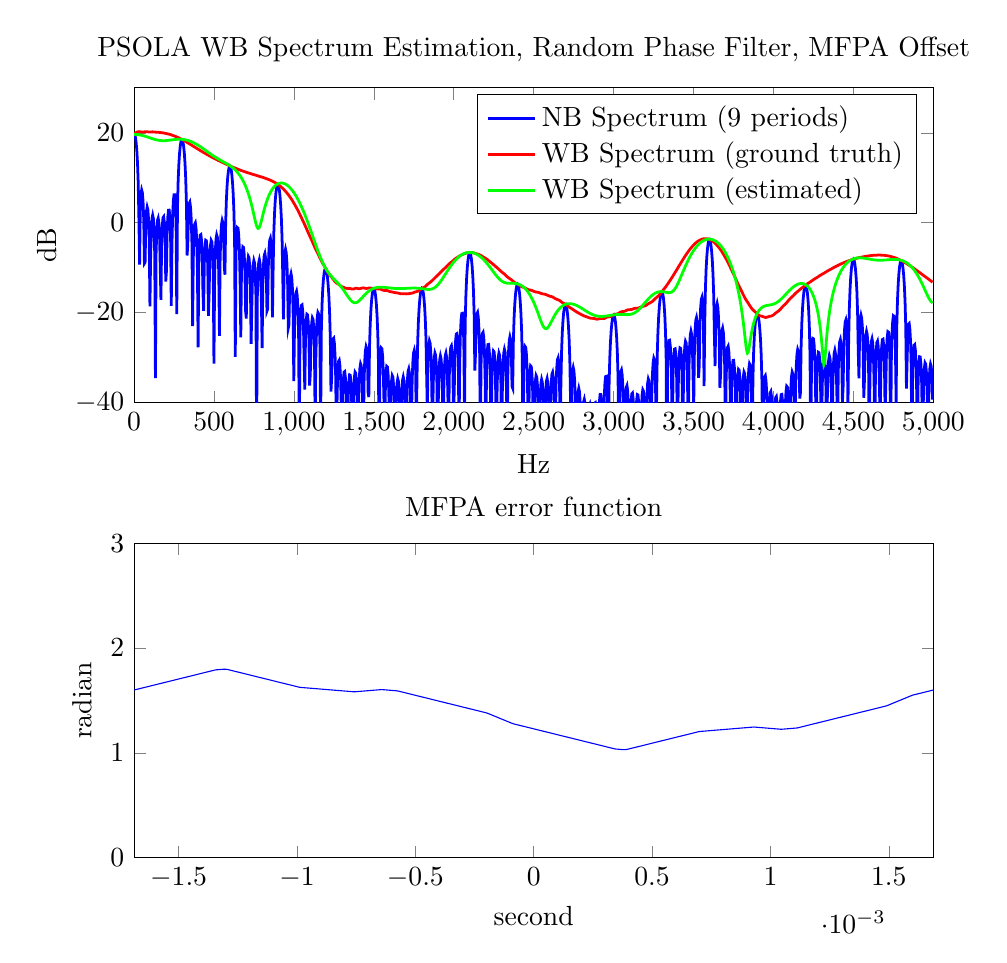
\begin{tikzpicture}

\begin{axis}[%
width=3.996in,
height=1.573in,
at={(0.67in,2.889in)},
scale only axis,
xmin=0,
xmax=5000,
xlabel={Hz},
ymin=-40,
ymax=30,
ylabel={dB},
axis background/.style={fill=white},
title={PSOLA WB Spectrum Estimation, Random Phase Filter, MFPA Offset},
legend style={legend cell align=left,align=left,legend plot pos=left,draw=black}
]
\addplot [color=blue,solid,line width=1.0pt]
  table[row sep=crcr]{%
0	19.8593346054116\\
4.306640625	19.6470766684657\\
8.61328125	18.986274809714\\
12.919921875	17.8023900607479\\
17.2265625	15.9552691820529\\
21.533203125	13.180537695682\\
25.83984375	8.86661639634541\\
30.146484375	0.759447616692297\\
34.453125	-9.332785667657\\
38.759765625	3.01442938954317\\
43.06640625	6.33169751815378\\
47.373046875	7.27926408339512\\
51.6796875	6.74096435230323\\
55.986328125	4.7702113524545\\
60.29296875	0.729897031676244\\
64.599609375	-9.06739986575636\\
68.90625	-8.82729471518252\\
73.212890625	-0.418883145778642\\
77.51953125	2.56946206751992\\
81.826171875	3.48914062151455\\
86.1328125	2.92848316932768\\
90.439453125	0.807147514354875\\
94.74609375	-3.82168929785955\\
99.052734375	-18.6004253206077\\
103.359375	-7.95129128477037\\
107.666015625	-1.59488202972874\\
111.97265625	0.951519944529689\\
116.279296875	1.67178420249874\\
120.5859375	0.928980236676468\\
124.892578125	-1.51745730978354\\
129.19921875	-7.11592771881383\\
133.505859375	-34.5801181802834\\
137.8125	-6.62454539571562\\
142.119140625	-1.58003870301409\\
146.42578125	0.541667193591836\\
150.732421875	1.00846814542794\\
155.0390625	0.00956402167801747\\
159.345703125	-2.88245381414726\\
163.65234375	-9.97856675058532\\
167.958984375	-17.1938682438496\\
172.265625	-4.78035058609264\\
176.572265625	-0.635572213342473\\
180.87890625	1.12791552435017\\
185.185546875	1.34584483786065\\
189.4921875	0.0570622358819469\\
193.798828125	-3.40616894653224\\
198.10546875	-13.0838223755133\\
202.412109375	-10.8241123548345\\
206.71875	-2.22341762146196\\
211.025390625	1.28736036134444\\
215.33203125	2.78023534109459\\
219.638671875	2.80252007794013\\
223.9453125	1.24613893208606\\
228.251953125	-2.90116704854191\\
232.55859375	-18.5235973754877\\
236.865234375	-5.07437946200521\\
241.171875	1.67692543287334\\
245.478515625	4.82183083902853\\
249.78515625	6.21884502657865\\
254.091796875	6.21344316618114\\
258.3984375	4.54902151417186\\
262.705078125	-0.313172227836078\\
267.01171875	-20.3588903487011\\
271.318359375	3.06131970138439\\
275.625	9.28099190014526\\
279.931640625	12.9384014511283\\
284.23828125	15.3589574420374\\
288.544921875	16.9745819143833\\
292.8515625	17.9752028843738\\
297.158203125	18.4529613251704\\
301.46484375	18.4483724573271\\
305.771484375	17.9663555890338\\
310.078125	16.9781804953973\\
314.384765625	15.4109298083725\\
318.69140625	13.114531519697\\
322.998046875	9.76421522356001\\
327.3046875	4.48287112002659\\
331.611328125	-7.28915823754944\\
335.91796875	-4.9641561665126\\
340.224609375	1.99762131989269\\
344.53125	4.24016109828536\\
348.837890625	4.5672751836391\\
353.14453125	3.4761046816148\\
357.451171875	0.824274994718987\\
361.7578125	-4.47766479182169\\
366.064453125	-22.9871894100464\\
370.37109375	-7.92968361570206\\
374.677734375	-2.40443558874503\\
378.984375	-0.346087356851279\\
383.291015625	-0.0337913042733417\\
387.59765625	-1.16210097745387\\
391.904296875	-4.02872728691059\\
396.2109375	-10.3018030252654\\
400.517578125	-27.7406561995673\\
404.82421875	-8.95738317062813\\
409.130859375	-4.50057833605844\\
413.4375	-2.76959553107098\\
417.744140625	-2.64817021652354\\
422.05078125	-3.99319637131741\\
426.357421875	-7.29934663416539\\
430.6640625	-15.2784849930523\\
434.970703125	-19.6256305767783\\
439.27734375	-8.99374596176916\\
443.583984375	-5.32210039517835\\
447.890625	-3.90712766515925\\
452.197265625	-4.01131670320744\\
456.50390625	-5.63960305436021\\
460.810546875	-9.55280361984487\\
465.1171875	-20.7182904198084\\
469.423828125	-15.792789001671\\
473.73046875	-8.16917574371243\\
478.037109375	-5.08994686090302\\
482.34375	-3.95341460869142\\
486.650390625	-4.28173699472497\\
490.95703125	-6.22874492800402\\
495.263671875	-10.9467752816124\\
499.5703125	-31.3693476739829\\
503.876953125	-12.2956342474966\\
508.18359375	-6.30890338251877\\
512.490234375	-3.65806415867343\\
516.796875	-2.73342069721743\\
521.103515625	-3.25062208935312\\
525.41015625	-5.52804743025243\\
529.716796875	-11.3482009730171\\
534.0234375	-25.1925889360795\\
538.330078125	-7.88815132235102\\
542.63671875	-2.8327490892964\\
546.943359375	-0.383336641094229\\
551.25	0.51346833759863\\
555.556640625	-0.012303638082457\\
559.86328125	-2.47547139389484\\
564.169921875	-9.80154058755646\\
568.4765625	-11.5655649684368\\
572.783203125	-0.267881669034237\\
577.08984375	4.79788594350516\\
581.396484375	7.96660497742971\\
585.703125	10.0931072388037\\
590.009765625	11.4952721979864\\
594.31640625	12.3202117443089\\
598.623046875	12.639808287411\\
602.9296875	12.4829286915673\\
607.236328125	11.8452886997728\\
611.54296875	10.6867717131777\\
615.849609375	8.91461371761619\\
620.15625	6.3360858109213\\
624.462890625	2.51060127598473\\
628.76953125	-3.9264970958489\\
633.076171875	-29.8699764401462\\
637.3828125	-7.2141167510655\\
641.689453125	-2.58392826723841\\
645.99609375	-1.08406020592237\\
650.302734375	-1.2286199883121\\
654.609375	-2.77412641139473\\
658.916015625	-6.08035075347264\\
663.22265625	-13.0744766501752\\
667.529296875	-25.4888922745812\\
671.8359375	-10.7640271398821\\
676.142578125	-6.79418213834048\\
680.44921875	-5.37057600641427\\
684.755859375	-5.51465747166746\\
689.0625	-7.1315311122338\\
693.369140625	-10.7887162673259\\
697.67578125	-19.6973247385728\\
701.982421875	-21.3386109753394\\
706.2890625	-12.0273714480262\\
710.595703125	-8.70507389456911\\
714.90234375	-7.52552991630434\\
719.208984375	-7.84414273751177\\
723.515625	-9.71352360296246\\
727.822265625	-13.9991338769947\\
732.12890625	-26.9681252466484\\
736.435546875	-18.9724135597049\\
740.7421875	-12.1011593290103\\
745.048828125	-9.32219248885633\\
749.35546875	-8.411809606689\\
753.662109375	-8.96009418001901\\
757.96875	-11.1725679011728\\
762.275390625	-16.3651204050642\\
766.58203125	-50.4033637575311\\
770.888671875	-16.6454433582187\\
775.1953125	-11.2182619719317\\
779.501953125	-8.879325335888\\
783.80859375	-8.22362304872384\\
788.115234375	-9.02108755214907\\
792.421875	-11.6518982957416\\
796.728515625	-18.1820357938765\\
801.03515625	-27.8777307875416\\
805.341796875	-13.7839565821593\\
809.6484375	-9.2918697964324\\
813.955078125	-7.27909871164222\\
818.26171875	-6.82222429053385\\
822.568359375	-7.84440708243888\\
826.875	-10.9482030264291\\
831.181640625	-19.6417147580596\\
835.48828125	-19.2179635103798\\
839.794921875	-9.70840578203416\\
844.1015625	-5.77026526934155\\
848.408203125	-3.89198150980169\\
852.71484375	-3.45971774468679\\
857.021484375	-4.53567023948208\\
861.328125	-8.0257594005086\\
865.634765625	-21.0474356253285\\
869.94140625	-10.1015481649554\\
874.248046875	-2.19959317827866\\
878.5546875	2.03431221060335\\
882.861328125	4.77327991030721\\
887.16796875	6.60533527266395\\
891.474609375	7.7717927339639\\
895.78125	8.38818932142929\\
900.087890625	8.50915044120241\\
904.39453125	8.15087262548289\\
908.701171875	7.29655736155056\\
913.0078125	5.88996456371056\\
917.314453125	3.81162973363836\\
921.62109375	0.811038191080835\\
925.927734375	-3.72703921020973\\
930.234375	-12.1390578627114\\
934.541015625	-21.4804163653411\\
938.84765625	-9.79192757612619\\
943.154296875	-6.68241374279732\\
947.4609375	-5.91921294684327\\
951.767578125	-6.65308647478354\\
956.07421875	-8.84436419718319\\
960.380859375	-13.1492314337111\\
964.6875	-23.4302079868201\\
968.994140625	-22.709719872331\\
973.30078125	-14.7501419239065\\
977.607421875	-12.0349842656813\\
981.9140625	-11.3626269287965\\
986.220703125	-12.1697540748552\\
990.52734375	-14.554974476215\\
994.833984375	-19.501608760052\\
999.140625	-35.2461559629583\\
1003.447265625	-23.806533300865\\
1007.75390625	-17.8632130332312\\
1012.060546875	-15.6433421617602\\
1016.3671875	-15.2322609153767\\
1020.673828125	-16.2822360261568\\
1024.98046875	-19.0506267900237\\
1029.287109375	-25.0414616782726\\
1033.59375	-49.0489298744527\\
1037.900390625	-24.8171151299565\\
1042.20703125	-20.1782560462964\\
1046.513671875	-18.4108810169655\\
1050.8203125	-18.2845334540309\\
1055.126953125	-19.6214733178922\\
1059.43359375	-22.8684372757492\\
1063.740234375	-30.4349837414352\\
1068.046875	-37.1480624115628\\
1072.353515625	-25.5073237656607\\
1076.66015625	-21.7657194537968\\
1080.966796875	-20.3725678008261\\
1085.2734375	-20.5113310632653\\
1089.580078125	-22.1494496224589\\
1093.88671875	-25.9766465965147\\
1098.193359375	-36.246288353504\\
1102.5	-33.5650057793056\\
1106.806640625	-25.4702794819571\\
1111.11328125	-22.3217866457233\\
1115.419921875	-21.1766826783217\\
1119.7265625	-21.5004356503055\\
1124.033203125	-23.4048451826168\\
1128.33984375	-27.9287040094997\\
1132.646484375	-44.7341927402474\\
1136.953125	-30.2983048216781\\
1141.259765625	-23.9262840157376\\
1145.56640625	-21.0760404470286\\
1149.873046875	-19.9612769230245\\
1154.1796875	-20.2540205478574\\
1158.486328125	-22.223379481286\\
1162.79296875	-27.4586537681424\\
1167.099609375	-45.6013997986615\\
1171.40625	-24.237642631607\\
1175.712890625	-18.3248522419297\\
1180.01953125	-14.9044661815224\\
1184.326171875	-12.691793179793\\
1188.6328125	-11.2699599312654\\
1192.939453125	-10.4599883957339\\
1197.24609375	-10.1773138841684\\
1201.552734375	-10.3839440850664\\
1205.859375	-11.0714974932496\\
1210.166015625	-12.260252197589\\
1214.47265625	-14.0129064996943\\
1218.779296875	-16.4725997793245\\
1223.0859375	-19.9670173030423\\
1227.392578125	-25.4005568635528\\
1231.69921875	-37.5880965555066\\
1236.005859375	-34.6095683821682\\
1240.3125	-27.9348656702638\\
1244.619140625	-25.8582373435688\\
1248.92578125	-25.683528706939\\
1253.232421875	-26.9159890984295\\
1257.5390625	-29.6938533130863\\
1261.845703125	-35.1332293602676\\
1266.15234375	-54.8869938116769\\
1270.458984375	-38.2663073589712\\
1274.765625	-32.8577894465962\\
1279.072265625	-30.8514174151236\\
1283.37890625	-30.5909349562815\\
1287.685546875	-31.778892032197\\
1291.9921875	-34.7145473825549\\
1296.298828125	-41.1146074324882\\
1300.60546875	-56.9831739775081\\
1304.912109375	-39.3839340079102\\
1309.21875	-34.9722602414761\\
1313.525390625	-33.2423355395328\\
1317.83203125	-33.1170096619685\\
1322.138671875	-34.460716225438\\
1326.4453125	-37.7766615257435\\
1330.751953125	-45.8844986384872\\
1335.05859375	-49.4140706504964\\
1339.365234375	-39.0236581091408\\
1343.671875	-35.3219422623663\\
1347.978515625	-33.8615203805433\\
1352.28515625	-33.9346351933726\\
1356.591796875	-35.5531776289138\\
1360.8984375	-39.4896849158063\\
1365.205078125	-50.9824766665152\\
1369.51171875	-45.2010957543147\\
1373.818359375	-37.6378140016031\\
1378.125	-34.4764153065035\\
1382.431640625	-33.2367733939659\\
1386.73828125	-33.4763881596424\\
1391.044921875	-35.3726491799865\\
1395.3515625	-40.1169393469357\\
1399.658203125	-62.3297224810393\\
1403.96484375	-41.038731015403\\
1408.271484375	-35.1021067154646\\
1412.578125	-32.4049105768008\\
1416.884765625	-31.3938255726395\\
1421.19140625	-31.8101434649748\\
1425.498046875	-34.0048863713317\\
1429.8046875	-39.8439124124438\\
1434.111328125	-52.3649775677514\\
1438.41796875	-35.9108415764449\\
1442.724609375	-30.9035515648031\\
1447.03125	-28.4592420790183\\
1451.337890625	-27.5412385639786\\
1455.64453125	-28.0223448082394\\
1459.951171875	-30.4388052979508\\
1464.2578125	-37.8600226117026\\
1468.564453125	-38.8032641982388\\
1472.87109375	-27.7162206209526\\
1477.177734375	-22.6501683546774\\
1481.484375	-19.4723450617374\\
1485.791015625	-17.3350331009931\\
1490.09765625	-15.9113573682199\\
1494.404296875	-15.0477489190737\\
1498.7109375	-14.6744243011193\\
1503.017578125	-14.7722253437805\\
1507.32421875	-15.3572926702582\\
1511.630859375	-16.4775536088382\\
1515.9375	-18.2261679646473\\
1520.244140625	-20.7906247399256\\
1524.55078125	-24.6096459297433\\
1528.857421875	-31.0824962855242\\
1533.1640625	-60.4347696785829\\
1537.470703125	-33.9087175578689\\
1541.77734375	-29.3399074112064\\
1546.083984375	-27.8614578865099\\
1550.390625	-28.0350725088891\\
1554.697265625	-29.6177611323648\\
1559.00390625	-32.9679344486359\\
1563.310546875	-40.0737304893832\\
1567.6171875	-51.3845912314525\\
1571.923828125	-37.3078224679822\\
1576.23046875	-33.3601155044655\\
1580.537109375	-31.9355262427765\\
1584.84375	-32.0918627521737\\
1589.150390625	-33.7415017536353\\
1593.45703125	-37.461074618364\\
1597.763671875	-46.5991970377023\\
1602.0703125	-47.5285640413205\\
1606.376953125	-38.4644355096551\\
1610.68359375	-35.1796952067889\\
1614.990234375	-34.0147420882645\\
1619.296875	-34.3487484269899\\
1623.603515625	-36.2437208135641\\
1627.91015625	-40.5885026317421\\
1632.216796875	-54.0659034089588\\
1636.5234375	-45.1511662193199\\
1640.830078125	-38.3983489819416\\
1645.13671875	-35.6393957045005\\
1649.443359375	-34.7408945985458\\
1653.75	-35.3105040539591\\
1658.056640625	-37.5623193933281\\
1662.36328125	-42.8489281038401\\
1666.669921875	-105.00620747869\\
1670.9765625	-42.7485958261364\\
1675.283203125	-37.3745772449786\\
1679.58984375	-35.0202604587396\\
1683.896484375	-34.3368225578162\\
1688.203125	-35.115350835072\\
1692.509765625	-37.7549881836987\\
1696.81640625	-44.3988424741782\\
1701.123046875	-53.1280943956726\\
1705.4296875	-39.5695381781624\\
1709.736328125	-35.0958553955736\\
1714.04296875	-33.0500947624224\\
1718.349609375	-32.5431187697697\\
1722.65625	-33.5163269255626\\
1726.962890625	-36.5976630888949\\
1731.26953125	-45.4644097776727\\
1735.576171875	-44.2573911513184\\
1739.8828125	-34.8937533336391\\
1744.189453125	-30.9041931763623\\
1748.49609375	-28.9357271113484\\
1752.802734375	-28.4014336133405\\
1757.109375	-29.3841252327372\\
1761.416015625	-32.8261408757153\\
1765.72265625	-46.3693479059954\\
1770.029296875	-34.3101450293724\\
1774.3359375	-26.4133027437242\\
1778.642578125	-22.0651777663371\\
1782.94921875	-19.1637236230608\\
1787.255859375	-17.1389723439664\\
1791.5625	-15.7663581747446\\
1795.869140625	-14.9459220940021\\
1800.17578125	-14.63255500356\\
1804.482421875	-14.8103570654124\\
1808.7890625	-15.4878698935034\\
1813.095703125	-16.7089082153487\\
1817.40234375	-18.5828305684745\\
1821.708984375	-21.3589100074946\\
1826.015625	-25.6684967400573\\
1830.322265625	-33.9442357631557\\
1834.62890625	-42.1376847054668\\
1838.935546875	-30.6364594741303\\
1843.2421875	-27.3061165390782\\
1847.548828125	-26.2882521798736\\
1851.85546875	-26.7550654832247\\
1856.162109375	-28.6723649276354\\
1860.46875	-32.7146656042013\\
1864.775390625	-42.9386705541845\\
1869.08203125	-41.1586011047384\\
1873.388671875	-33.0534286338037\\
1877.6953125	-30.0231717255367\\
1882.001953125	-29.0066953005895\\
1886.30859375	-29.4604896652432\\
1890.615234375	-31.4947358483366\\
1894.921875	-36.1247461605528\\
1899.228515625	-52.264762497199\\
1903.53515625	-39.2689462578903\\
1907.841796875	-33.0380840709171\\
1912.1484375	-30.4368717338176\\
1916.455078125	-29.6194221961028\\
1920.76171875	-30.2533310417321\\
1925.068359375	-32.6112586116293\\
1929.375	-38.2531783072659\\
1933.681640625	-59.0939330471099\\
1937.98828125	-36.7723546280088\\
1942.294921875	-31.7638912239436\\
1946.6015625	-29.5742957852485\\
1950.908203125	-29.0103587804043\\
1955.21484375	-29.904353750814\\
1959.521484375	-32.7195201566249\\
1963.828125	-39.9661545016302\\
1968.134765625	-45.3973663852904\\
1972.44140625	-33.6815822969092\\
1976.748046875	-29.5256044785766\\
1981.0546875	-27.6922591596885\\
1985.361328125	-27.3897872828515\\
1989.66796875	-28.5948906527341\\
1993.974609375	-32.0184951024868\\
1998.28125	-42.1389051515305\\
2002.587890625	-38.2680387530637\\
2006.89453125	-29.9077040699261\\
2011.201171875	-26.3516160647804\\
2015.5078125	-24.7805378043758\\
2019.814453125	-24.679105243819\\
2024.12109375	-26.1727921058266\\
2028.427734375	-30.3382306899175\\
2032.734375	-47.7599397934706\\
2037.041015625	-31.5223159560725\\
2041.34765625	-24.8743519653696\\
2045.654296875	-21.6822384967924\\
2049.9609375	-20.2167957826606\\
2054.267578125	-20.1579985093104\\
2058.57421875	-21.7851458246594\\
2062.880859375	-26.7467844739458\\
2067.1875	-42.708700428162\\
2071.494140625	-22.428117650123\\
2075.80078125	-16.2517205034108\\
2080.107421875	-12.5477848349798\\
2084.4140625	-10.0653772562342\\
2088.720703125	-8.38683419825366\\
2093.02734375	-7.32366190484037\\
2097.333984375	-6.78153295337568\\
2101.640625	-6.71822705553682\\
2105.947265625	-7.12976629485986\\
2110.25390625	-8.04903307402283\\
2114.560546875	-9.55574160469931\\
2118.8671875	-11.8089752887951\\
2123.173828125	-15.147817021202\\
2127.48046875	-20.4935904491254\\
2131.787109375	-32.9100769045871\\
2136.09375	-29.0508215642451\\
2140.400390625	-22.4171458907248\\
2144.70703125	-20.2349461493618\\
2149.013671875	-19.9256469649922\\
2153.3203125	-21.0295818274495\\
2157.626953125	-23.7169006786438\\
2161.93359375	-29.1544630601029\\
2166.240234375	-50.3404786472752\\
2170.546875	-31.8885573733423\\
2174.853515625	-26.5942818768441\\
2179.16015625	-24.6268274720394\\
2183.466796875	-24.3791704725582\\
2187.7734375	-25.5703803393316\\
2192.080078125	-28.5254098200734\\
2196.38671875	-35.0378142404274\\
2200.693359375	-49.5428970333926\\
2205	-33.0134054815425\\
2209.306640625	-28.7376166647358\\
2213.61328125	-27.1084159145723\\
2217.919921875	-27.0782027772328\\
2222.2265625	-28.5240904029466\\
2226.533203125	-31.973446155842\\
2230.83984375	-40.3760733422849\\
2235.146484375	-43.2967117238772\\
2239.453125	-33.3493502412746\\
2243.759765625	-29.8402208361422\\
2248.06640625	-28.5348041978055\\
2252.373046875	-28.7422032453588\\
2256.6796875	-30.4884236519819\\
2260.986328125	-34.5832900040212\\
2265.29296875	-46.5956072135715\\
2269.599609375	-40.1526799120645\\
2273.90625	-32.9212289619993\\
2278.212890625	-29.9988807674174\\
2282.51953125	-28.9867621626858\\
2286.826171875	-29.4391488926382\\
2291.1328125	-31.5302277667953\\
2295.439453125	-36.4865571946834\\
2299.74609375	-61.2209404443787\\
2304.052734375	-37.2553728178305\\
2308.359375	-31.5296776150368\\
2312.666015625	-29.0081456981926\\
2316.97265625	-28.1950444957751\\
2321.279296875	-28.8354800083602\\
2325.5859375	-31.2750064812108\\
2329.892578125	-37.4257390383538\\
2334.19921875	-48.952819225345\\
2338.505859375	-33.3940907005838\\
2342.8125	-28.5393213463134\\
2347.119140625	-26.1964438496571\\
2351.42578125	-25.3846404007613\\
2355.732421875	-26.0052515727064\\
2360.0390625	-28.6170587935093\\
2364.345703125	-36.417668633194\\
2368.65234375	-36.8163491943689\\
2372.958984375	-26.1513424356924\\
2377.265625	-21.2521136781406\\
2381.572265625	-18.1773385057562\\
2385.87890625	-16.110136756904\\
2390.185546875	-14.7466392148609\\
2394.4921875	-13.9512154038707\\
2398.798828125	-13.6626195038095\\
2403.10546875	-13.8599295872399\\
2407.412109375	-14.5508036444942\\
2411.71875	-15.7737572192914\\
2416.025390625	-17.6168472438903\\
2420.33203125	-20.269842930392\\
2424.638671875	-24.1836034268352\\
2428.9453125	-30.8029167724257\\
2433.251953125	-66.4019714005567\\
2437.55859375	-33.3831879478861\\
2441.865234375	-28.948423113485\\
2446.171875	-27.532640569931\\
2450.478515625	-27.7513154816539\\
2454.78515625	-29.3830933938642\\
2459.091796875	-32.8094662986436\\
2463.3984375	-40.0970690820892\\
2467.705078125	-50.467332372006\\
2472.01171875	-37.068751427296\\
2476.318359375	-33.2257025076207\\
2480.625	-31.8486476227795\\
2484.931640625	-32.0301219103789\\
2489.23828125	-33.705020298871\\
2493.544921875	-37.4820943252284\\
2497.8515625	-46.8750563107116\\
2502.158203125	-47.1308915015191\\
2506.46484375	-38.3474069601743\\
2510.771484375	-35.1404477853439\\
2515.078125	-34.0119522756382\\
2519.384765625	-34.3636517375758\\
2523.69140625	-36.2788761203418\\
2527.998046875	-40.6890249019881\\
2532.3046875	-54.7565052285587\\
2536.611328125	-44.9340207731503\\
2540.91796875	-38.3705088203464\\
2545.224609375	-35.7040339715248\\
2549.53125	-34.8673631450748\\
2553.837890625	-35.4764884901794\\
2558.14453125	-37.7611091133876\\
2562.451171875	-43.1324081573405\\
2566.7578125	-76.1700499071185\\
2571.064453125	-42.7052868712779\\
2575.37109375	-37.4723184388708\\
2579.677734375	-35.2269441486249\\
2583.984375	-34.6533440754984\\
2588.291015625	-35.54020708217\\
2592.59765625	-38.2905171150896\\
2596.904296875	-45.1276943716112\\
2601.2109375	-52.9977374744025\\
2605.517578125	-39.9911606084764\\
2609.82421875	-35.6288232785052\\
2614.130859375	-33.680830258747\\
2618.4375	-33.289536242224\\
2622.744140625	-34.403873510457\\
2627.05078125	-37.6644405259101\\
2631.357421875	-46.9204612657217\\
2635.6640625	-45.1291319198479\\
2639.970703125	-36.1056215033195\\
2644.27734375	-32.2815854800702\\
2648.583984375	-30.456208457312\\
2652.890625	-30.0664203832675\\
2657.197265625	-31.2095453149559\\
2661.50390625	-34.8611906356653\\
2665.810546875	-49.260211999239\\
2670.1171875	-36.2939839737482\\
2674.423828125	-28.7016425884531\\
2678.73046875	-24.580976079877\\
2683.037109375	-21.8974311753154\\
2687.34375	-20.0870763646473\\
2691.650390625	-18.9230923415622\\
2695.95703125	-18.3035963556727\\
2700.263671875	-18.1850552878734\\
2704.5703125	-18.5570316584675\\
2708.876953125	-19.4357336226253\\
2713.18359375	-20.8721590766889\\
2717.490234375	-22.9801878684369\\
2721.796875	-26.0113372755835\\
2726.103515625	-30.6049546511673\\
2730.41015625	-39.2790517323944\\
2734.716796875	-46.8868912081727\\
2739.0234375	-36.0565047676951\\
2743.330078125	-33.016838820535\\
2747.63671875	-32.2553746209445\\
2751.943359375	-32.9750135254448\\
2756.25	-35.1555622573567\\
2760.556640625	-39.4945058520689\\
2764.86328125	-50.2569217641402\\
2769.169921875	-48.0044123804479\\
2773.4765625	-40.3485876048246\\
2777.783203125	-37.6128311072675\\
2782.08984375	-36.8648408659752\\
2786.396484375	-37.5794314916577\\
2790.703125	-39.8792966591335\\
2795.009765625	-44.8148028792416\\
2799.31640625	-62.0877268366828\\
2803.623046875	-48.0625875648403\\
2807.9296875	-42.1848420709088\\
2812.236328125	-39.8567774696264\\
2816.54296875	-39.2961321351292\\
2820.849609375	-40.181558693505\\
2825.15625	-42.7965206258356\\
2829.462890625	-48.7558855395425\\
2833.76953125	-67.6555098043991\\
2838.076171875	-47.3315717461109\\
2842.3828125	-42.6081152478516\\
2846.689453125	-40.6575496129373\\
2850.99609375	-40.3239238654966\\
2855.302734375	-41.4470785142775\\
2859.609375	-44.5011937958122\\
2863.916015625	-52.0960084439547\\
2868.22265625	-56.9161579782458\\
2872.529296875	-45.7317509402201\\
2876.8359375	-41.7885542354611\\
2881.142578125	-40.1427232331651\\
2885.44921875	-40.0303520492363\\
2889.755859375	-41.4353261623535\\
2894.0625	-45.0820832879825\\
2898.369140625	-55.6812393508308\\
2902.67578125	-51.1881792532209\\
2906.982421875	-43.106376082989\\
2911.2890625	-39.6762880434304\\
2915.595703125	-38.2098208205692\\
2919.90234375	-38.2232262122974\\
2924.208984375	-39.8595877625833\\
2928.515625	-44.2258187205749\\
2932.822265625	-62.9921825501929\\
2937.12890625	-45.2738528810139\\
2941.435546875	-38.8002230871288\\
2945.7421875	-35.6697063774259\\
2950.048828125	-34.2243062951739\\
2954.35546875	-34.1774522647659\\
2958.662109375	-35.8421259524685\\
2962.96875	-40.939078573157\\
2967.275390625	-55.3900323608551\\
2971.58203125	-36.3630249381073\\
2975.888671875	-30.3042324482321\\
2980.1953125	-26.6401730463197\\
2984.501953125	-24.1441430954241\\
2988.80859375	-22.4093163074146\\
2993.115234375	-21.2649081185316\\
2997.421875	-20.6384380811829\\
3001.728515625	-20.506512554802\\
3006.03515625	-20.8746758611793\\
3010.341796875	-21.7733848762201\\
3014.6484375	-23.2698926232029\\
3018.955078125	-25.5068326961345\\
3023.26171875	-28.8125212590397\\
3027.568359375	-34.1232503769736\\
3031.875	-46.7940005346412\\
3036.181640625	-42.0140647141124\\
3040.48828125	-35.4068984853904\\
3044.794921875	-33.1459013738736\\
3049.1015625	-32.7643721036974\\
3053.408203125	-33.8170125923414\\
3057.71484375	-36.4734686098061\\
3062.021484375	-41.9215442698902\\
3066.328125	-64.857719674683\\
3070.634765625	-44.0828308141825\\
3074.94140625	-38.7387017599075\\
3079.248046875	-36.6377587337947\\
3083.5546875	-36.2464436558861\\
3087.861328125	-37.3132806790195\\
3092.16796875	-40.1851954492572\\
3096.474609375	-46.7185357819219\\
3100.78125	-59.8863713418094\\
3105.087890625	-44.1482117956347\\
3109.39453125	-39.8269901975053\\
3113.701171875	-38.0817682557414\\
3118.0078125	-37.9025822754143\\
3122.314453125	-39.1908994264135\\
3126.62109375	-42.5083852174577\\
3130.927734375	-50.9483340990407\\
3135.234375	-53.0045363060396\\
3139.541015625	-43.2191205189885\\
3143.84765625	-39.6420742745509\\
3148.154296875	-38.2343321937171\\
3152.4609375	-38.31794796782\\
3156.767578125	-39.9269177125984\\
3161.07421875	-43.9008188371507\\
3165.380859375	-56.1615792805697\\
3169.6875	-48.695770767769\\
3173.994140625	-41.4292989452006\\
3178.30078125	-38.3684228146835\\
3182.607421875	-37.2064436236129\\
3186.9140625	-37.5104322603686\\
3191.220703125	-39.4619490745017\\
3195.52734375	-44.324342386254\\
3199.833984375	-72.3923722034662\\
3204.140625	-44.3497042223025\\
3208.447265625	-38.508211668137\\
3212.75390625	-35.7990681389345\\
3217.060546875	-34.7819121049017\\
3221.3671875	-35.2198721947778\\
3225.673828125	-37.4770131004812\\
3229.98046875	-43.5392487927682\\
3234.287109375	-53.7902146900282\\
3238.59375	-38.711772061193\\
3242.900390625	-33.7039140621303\\
3247.20703125	-31.1574393936798\\
3251.513671875	-30.1216839461902\\
3255.8203125	-30.5117925702876\\
3260.126953125	-32.9107099614191\\
3264.43359375	-40.6697055401202\\
3268.740234375	-40.0981613469546\\
3273.046875	-29.4343011190198\\
3277.353515625	-24.3327171285475\\
3281.66015625	-21.02832407761\\
3285.966796875	-18.7197574367557\\
3290.2734375	-17.1053177312474\\
3294.580078125	-16.0495393873016\\
3298.88671875	-15.4916546436144\\
3303.193359375	-15.4121272552097\\
3307.5	-15.8211058464249\\
3311.806640625	-16.760823401963\\
3316.11328125	-18.3243586101523\\
3320.419921875	-20.7081222596708\\
3324.7265625	-24.3742017719656\\
3329.033203125	-30.810880546222\\
3333.33984375	-87.90607647463\\
3337.646484375	-32.5023850324611\\
3341.953125	-27.8823000113036\\
3346.259765625	-26.2105487478504\\
3350.56640625	-26.1490966041354\\
3354.873046875	-27.4937038084297\\
3359.1796875	-30.6490528995852\\
3363.486328125	-37.7703712169102\\
3367.79296875	-46.9090836309277\\
3372.099609375	-33.7991336506917\\
3376.40625	-29.7527090616647\\
3380.712890625	-28.1349599333456\\
3385.01953125	-28.059038711499\\
3389.326171875	-29.4662822885431\\
3393.6328125	-32.9867538119549\\
3397.939453125	-42.3098554293474\\
3402.24609375	-41.5434651589063\\
3406.552734375	-32.6870845480705\\
3410.859375	-29.2407137632173\\
3415.166015625	-27.8630153926244\\
3419.47265625	-27.9702001566615\\
3423.779296875	-29.6489764186699\\
3428.0859375	-33.8538106313413\\
3432.392578125	-48.2712180621029\\
3436.69921875	-37.1522201658252\\
3441.005859375	-30.4247721576897\\
3445.3125	-27.5067787922715\\
3449.619140625	-26.4140150118439\\
3453.92578125	-26.7813106707858\\
3458.232421875	-28.8504600344552\\
3462.5390625	-34.0767396666368\\
3466.845703125	-60.8312370801053\\
3471.15234375	-32.8192673268142\\
3475.458984375	-27.4258773257672\\
3479.765625	-24.9608675454126\\
3484.072265625	-24.1567430773883\\
3488.37890625	-24.8218552108221\\
3492.685546875	-27.382007342304\\
3496.9921875	-34.1533478693906\\
3501.298828125	-40.9690131975689\\
3505.60546875	-28.2508540496282\\
3509.912109375	-23.7716761263398\\
3514.21875	-21.670451868803\\
3518.525390625	-21.1126330322275\\
3522.83203125	-22.0588587308819\\
3527.138671875	-25.1767763762916\\
3531.4453125	-34.5192444999425\\
3535.751953125	-31.8408621619733\\
3540.05859375	-22.8771111805827\\
3544.365234375	-18.9744166881349\\
3548.671875	-17.0647136235622\\
3552.978515625	-16.5942517106421\\
3557.28515625	-17.6618746590734\\
3561.591796875	-21.2691507987728\\
3565.8984375	-36.3365278298344\\
3570.205078125	-22.0837638892501\\
3574.51171875	-14.4923292148138\\
3578.818359375	-10.3056520360124\\
3583.125	-7.56378856796503\\
3587.431640625	-5.71419818365814\\
3591.73828125	-4.52682821012044\\
3596.044921875	-3.8907679403945\\
3600.3515625	-3.75340841873472\\
3604.658203125	-4.09955772227428\\
3608.96484375	-4.94719495551135\\
3613.271484375	-6.35517573469121\\
3617.578125	-8.44882395653159\\
3621.884765625	-11.4923427438129\\
3626.19140625	-16.1433346445131\\
3630.498046875	-25.0163261295703\\
3634.8046875	-31.8814840516604\\
3639.111328125	-21.5214674090735\\
3643.41796875	-18.6132056363384\\
3647.724609375	-17.952816690885\\
3652.03125	-18.7699361731508\\
3656.337890625	-21.0595504948233\\
3660.64453125	-25.5469853120076\\
3664.951171875	-36.7274465835688\\
3669.2578125	-33.8674525574156\\
3673.564453125	-26.5432385428011\\
3677.87109375	-24.0101562540714\\
3682.177734375	-23.4561643115808\\
3686.484375	-24.3713764002949\\
3690.791015625	-26.8875978346218\\
3695.09765625	-32.0883961463531\\
3699.404296875	-50.6001239138561\\
3703.7109375	-35.375970378973\\
3708.017578125	-29.825652766112\\
3712.32421875	-27.760993850012\\
3716.630859375	-27.46560161575\\
3720.9375	-28.6330176222924\\
3725.244140625	-31.5577057211768\\
3729.55078125	-37.9064070948509\\
3733.857421875	-55.2957232294937\\
3738.1640625	-36.6854510650704\\
3742.470703125	-32.3111277119179\\
3746.77734375	-30.6615062142649\\
3751.083984375	-30.6264781855838\\
3755.390625	-32.067387806896\\
3759.697265625	-35.4819999884543\\
3764.00390625	-43.5893198411192\\
3768.310546875	-48.0012627869981\\
3772.6171875	-37.5138418129175\\
3776.923828125	-33.9582346715132\\
3781.23046875	-32.6449324139334\\
3785.537109375	-32.8368735159317\\
3789.84375	-34.5419603726995\\
3794.150390625	-38.5272539000732\\
3798.45703125	-49.7852078619901\\
3802.763671875	-44.8684748357239\\
3807.0703125	-37.3226415461403\\
3811.376953125	-34.3065508952582\\
3815.68359375	-33.2187738718865\\
3819.990234375	-33.5742346532552\\
3824.296875	-35.5206883295562\\
3828.603515625	-40.2097716934426\\
3832.91015625	-60.6868533208456\\
3837.216796875	-41.3716434975366\\
3841.5234375	-35.2737549938624\\
3845.830078125	-32.4828475545198\\
3850.13671875	-31.3888645761328\\
3854.443359375	-31.6971938643931\\
3858.75	-33.7094338747937\\
3863.056640625	-39.1898257343994\\
3867.36328125	-52.4813216765449\\
3871.669921875	-34.6526996806212\\
3875.9765625	-28.8280826027843\\
3880.283203125	-25.3605281257343\\
3884.58984375	-23.0762688559653\\
3888.896484375	-21.5822507943224\\
3893.203125	-20.7006473172361\\
3897.509765625	-20.33826943484\\
3901.81640625	-20.4464654441311\\
3906.123046875	-21.0108717833149\\
3910.4296875	-22.0552223156218\\
3914.736328125	-23.6564861806444\\
3919.04296875	-25.9811257412618\\
3923.349609375	-29.3897502074191\\
3927.65625	-34.8633325281865\\
3931.962890625	-48.0788100507417\\
3936.26953125	-42.6569811370891\\
3940.576171875	-36.3720288025237\\
3944.8828125	-34.2918289597175\\
3949.189453125	-34.0269315742014\\
3953.49609375	-35.1414875151057\\
3957.802734375	-37.8263674852406\\
3962.109375	-43.3314065871638\\
3966.416015625	-68.6924751521817\\
3970.72265625	-45.120373085756\\
3975.029296875	-39.9097481820142\\
3979.3359375	-37.897745409204\\
3983.642578125	-37.5827082075014\\
3987.94921875	-38.7022129878426\\
3992.255859375	-41.5995995556432\\
3996.5625	-48.1953513476701\\
4000.869140625	-60.1199786330326\\
4005.17578125	-45.0433671452409\\
4009.482421875	-40.6809953501478\\
4013.7890625	-38.8775435630712\\
4018.095703125	-38.6608466203186\\
4022.40234375	-39.9358296554396\\
4026.708984375	-43.265330991318\\
4031.015625	-51.8618383750723\\
4035.322265625	-53.1162166663544\\
4039.62890625	-43.478230939592\\
4043.935546875	-39.8003886283617\\
4048.2421875	-38.2547323736206\\
4052.548828125	-38.2059456669346\\
4056.85546875	-39.7153261390461\\
4061.162109375	-43.6553804209231\\
4065.46875	-56.3231563035086\\
4069.775390625	-47.9316970843081\\
4074.08203125	-40.740572173427\\
4078.388671875	-37.6262153132793\\
4082.6953125	-36.3662434573813\\
4087.001953125	-36.5514471579775\\
4091.30859375	-38.3922550156488\\
4095.615234375	-43.2142704874133\\
4099.921875	-77.5609157759612\\
4104.228515625	-42.7264317206765\\
4108.53515625	-36.9428670015548\\
4112.841796875	-34.2427988599219\\
4117.1484375	-33.217755995316\\
4121.455078125	-33.6322118005346\\
4125.76171875	-35.8635781544421\\
4130.068359375	-41.982690588727\\
4134.375	-51.1679810891721\\
4138.681640625	-36.6622936170873\\
4142.98828125	-31.7003460058276\\
4147.294921875	-29.1909924180343\\
4151.6015625	-28.2045688460028\\
4155.908203125	-28.6540830580974\\
4160.21484375	-31.1306651217727\\
4164.521484375	-39.1389914816297\\
4168.828125	-37.8669294191833\\
4173.134765625	-27.4538186045349\\
4177.44140625	-22.4200931090986\\
4181.748046875	-19.1750540322187\\
4186.0546875	-16.936900954979\\
4190.361328125	-15.4039601250909\\
4194.66796875	-14.4345047115636\\
4198.974609375	-13.9615033212945\\
4203.28125	-13.9630494114443\\
4207.587890625	-14.4519502914845\\
4211.89453125	-15.4767126956271\\
4216.201171875	-17.1376197063021\\
4220.5078125	-19.6373635981454\\
4224.814453125	-23.4462820874944\\
4229.12109375	-30.0940052869688\\
4233.427734375	-63.9060815621888\\
4237.734375	-31.6776099634197\\
4242.041015625	-27.2672532852973\\
4246.34765625	-25.7505017287498\\
4250.654296875	-25.8385008902839\\
4254.9609375	-27.3433368301407\\
4259.267578125	-30.686750567344\\
4263.57421875	-38.1066714040916\\
4267.880859375	-46.5111718583272\\
4272.1875	-34.0766755867485\\
4276.494140625	-30.2518479353643\\
4280.80078125	-28.8168569777312\\
4285.107421875	-28.9152914713248\\
4289.4140625	-30.5034331862686\\
4293.720703125	-34.2359090527803\\
4298.02734375	-43.9857355416235\\
4302.333984375	-42.6821154286172\\
4306.640625	-34.22229218336\\
4310.947265625	-31.0018613915737\\
4315.25390625	-29.823555393763\\
4319.560546875	-30.1213757795498\\
4323.8671875	-31.9936341618873\\
4328.173828125	-36.4277324462624\\
4332.48046875	-51.710774069118\\
4336.787109375	-39.6766706055442\\
4341.09375	-33.2368850715054\\
4345.400390625	-30.5195066918339\\
4349.70703125	-29.6110081010706\\
4354.013671875	-30.1588295155331\\
4358.3203125	-32.4156697650567\\
4362.626953125	-37.8862440779847\\
4366.93359375	-61.1248819240449\\
4371.240234375	-36.5463173265365\\
4375.546875	-31.362501439481\\
4379.853515625	-29.0498558386536\\
4384.16015625	-28.3833716886528\\
4388.466796875	-29.1841352411193\\
4392.7734375	-31.8941022845486\\
4397.080078125	-38.9223007804298\\
4401.38671875	-45.0091636124481\\
4405.693359375	-32.8149653739295\\
4410	-28.4773045457645\\
4414.306640625	-26.47554417908\\
4418.61328125	-26.0016325214953\\
4422.919921875	-27.0278238368299\\
4427.2265625	-30.2446944404312\\
4431.533203125	-39.9158139587978\\
4435.83984375	-36.5442599049321\\
4440.146484375	-27.8020171008353\\
4444.453125	-23.961711473047\\
4448.759765625	-22.0851900511943\\
4453.06640625	-21.6368709383668\\
4457.373046875	-22.7265986475699\\
4461.6796875	-26.388755524249\\
4465.986328125	-42.3334466779082\\
4470.29296875	-26.7750723303506\\
4474.599609375	-19.2522861922985\\
4478.90625	-15.0422376130894\\
4483.212890625	-12.250144284738\\
4487.51953125	-10.3353917619823\\
4491.826171875	-9.07212280270296\\
4496.1328125	-8.35131421270797\\
4500.439453125	-8.12116370252311\\
4504.74609375	-8.36665275298717\\
4509.052734375	-9.10564375590966\\
4513.359375	-10.3970574747738\\
4517.666015625	-12.3672924051811\\
4521.97265625	-15.2845874829959\\
4526.279296875	-19.8213773041197\\
4530.5859375	-28.6963225949319\\
4534.892578125	-34.6122523008595\\
4539.19921875	-24.4469531838663\\
4543.505859375	-21.4112056885833\\
4547.8125	-20.5858308598184\\
4552.119140625	-21.2247528302922\\
4556.42578125	-23.3332004030571\\
4560.732421875	-27.6592071713786\\
4565.0390625	-38.9425767382805\\
4569.345703125	-35.0994511641096\\
4573.65234375	-27.7096267289677\\
4577.958984375	-24.9667039585757\\
4582.265625	-24.1757313689809\\
4586.572265625	-24.8458050590187\\
4590.87890625	-27.1211911378081\\
4595.185546875	-32.1214103650836\\
4599.4921875	-51.5814823204219\\
4603.798828125	-34.4796814786985\\
4608.10546875	-28.7434755412787\\
4612.412109375	-26.4112524086842\\
4616.71875	-25.8271596176418\\
4621.025390625	-26.6997147596078\\
4625.33203125	-29.3389721286518\\
4629.638671875	-35.4743121890495\\
4633.9453125	-50.9888632292534\\
4638.251953125	-33.2457551257503\\
4642.55859375	-28.6245320300615\\
4646.865234375	-26.6841583928605\\
4651.171875	-26.3489190036625\\
4655.478515625	-27.4901231422033\\
4659.78515625	-30.6219400264443\\
4664.091796875	-38.5801736496545\\
4668.3984375	-41.9152769341451\\
4672.705078125	-31.4222113226116\\
4677.01171875	-27.5972060322841\\
4681.318359375	-25.9967943601298\\
4685.625	-25.9097771571854\\
4689.931640625	-27.3543064420949\\
4694.23828125	-31.1184507772551\\
4698.544921875	-42.4785684363111\\
4702.8515625	-36.5022211942617\\
4707.158203125	-28.8395358740576\\
4711.46484375	-25.5831541103925\\
4715.771484375	-24.2419866429776\\
4720.078125	-24.3567395147489\\
4724.384765625	-26.0944469381771\\
4728.69140625	-30.6481857830384\\
4732.998046875	-52.7917306602589\\
4737.3046875	-31.0806997464138\\
4741.611328125	-24.9097269518502\\
4745.91796875	-21.9739957067481\\
4750.224609375	-20.7165530233856\\
4754.53125	-20.8608212116277\\
4758.837890625	-22.7325590355733\\
4763.14453125	-28.1738011200249\\
4767.451171875	-40.0908283453855\\
4771.7578125	-23.0453324697219\\
4776.064453125	-17.2182292537967\\
4780.37109375	-13.7189446356193\\
4784.677734375	-11.3928785016459\\
4788.984375	-9.84509694337467\\
4793.291015625	-8.89830092381325\\
4797.59765625	-8.46655016783569\\
4801.904296875	-8.51402639424611\\
4806.2109375	-9.04059201207229\\
4810.517578125	-10.0804028983581\\
4814.82421875	-11.7132877495369\\
4819.130859375	-14.1008956140961\\
4823.4375	-17.5967838293379\\
4827.744140625	-23.1926277387019\\
4832.05078125	-36.9019376899088\\
4836.357421875	-30.6908559641069\\
4840.6640625	-24.5967873283579\\
4844.970703125	-22.6057979022391\\
4849.27734375	-22.4351434121666\\
4853.583984375	-23.6743780681408\\
4857.890625	-26.5271719701635\\
4862.197265625	-32.2768822851529\\
4866.50390625	-61.3911772198352\\
4870.810546875	-34.0515600128297\\
4875.1171875	-29.0951319370816\\
4879.423828125	-27.2633322711367\\
4883.73046875	-27.1130654178968\\
4888.037109375	-28.4075051551957\\
4892.34375	-31.5169276081289\\
4896.650390625	-38.4415075946679\\
4900.95703125	-49.533765979423\\
4905.263671875	-35.3957122857594\\
4909.5703125	-31.3551008544895\\
4913.876953125	-29.8298270959981\\
4918.18359375	-29.8729550184765\\
4922.490234375	-31.4018347553549\\
4926.796875	-35.0058830553926\\
4931.103515625	-44.0566037331007\\
4935.41015625	-44.849624361314\\
4939.716796875	-35.7375954607966\\
4944.0234375	-32.3990635007998\\
4948.330078125	-31.1784038310854\\
4952.63671875	-31.4516423281939\\
4956.943359375	-33.2828038509811\\
4961.25	-37.5683295801854\\
4965.556640625	-51.0299270699257\\
4969.86328125	-42.0005612613412\\
4974.169921875	-35.2184504886396\\
4978.4765625	-32.4217281807628\\
4982.783203125	-31.4749076603009\\
4987.08984375	-31.9826080648148\\
4991.396484375	-34.16173126589\\
4995.703125	-39.3751820424122\\
};
\addlegendentry{NB Spectrum (9 periods)};

\addplot [color=red,solid,line width=1.0pt]
  table[row sep=crcr]{%
0	19.8593346054116\\
4.306640625	19.8839524738542\\
8.61328125	19.9503594517554\\
12.919921875	20.0396835351192\\
17.2265625	20.1296013338487\\
21.533203125	20.201972828705\\
25.83984375	20.2469338171071\\
30.146484375	20.2631837579228\\
34.453125	20.2559059488285\\
38.759765625	20.2339478934417\\
43.06640625	20.2072880219475\\
47.373046875	20.1850500013049\\
51.6796875	20.1738684686099\\
55.986328125	20.1765242658626\\
60.29296875	20.1912420702654\\
64.599609375	20.2122589461967\\
68.90625	20.2318258190917\\
73.212890625	20.2430046440267\\
77.51953125	20.2421484708107\\
81.826171875	20.2301036561209\\
86.1328125	20.2117230504754\\
90.439453125	20.1938903150905\\
94.74609375	20.1827776197293\\
99.052734375	20.1814034277778\\
103.359375	20.1885305782035\\
107.666015625	20.1993978675746\\
111.97265625	20.2079103098082\\
116.279296875	20.2092353288657\\
120.5859375	20.2016466922446\\
124.892578125	20.1868904378288\\
129.19921875	20.1690298236526\\
133.505859375	20.1523806599498\\
137.8125	20.1395422497984\\
142.119140625	20.1304567603755\\
146.42578125	20.1228650154782\\
150.732421875	20.1137735287114\\
155.0390625	20.1010653427248\\
159.345703125	20.084419430332\\
163.65234375	20.0651475738199\\
167.958984375	20.0451406366455\\
172.265625	20.0255687188241\\
176.572265625	20.0060894953307\\
180.87890625	19.9850070180272\\
185.185546875	19.9602554998256\\
189.4921875	19.9306122464911\\
193.798828125	19.8964483622049\\
198.10546875	19.859614495346\\
202.412109375	19.8225311404046\\
206.71875	19.7869628909622\\
211.025390625	19.7531121428369\\
215.33203125	19.7194910224133\\
219.638671875	19.6836128517565\\
223.9453125	19.6431258775024\\
228.251953125	19.5968238647253\\
232.55859375	19.5450792249593\\
236.865234375	19.4895533542587\\
241.171875	19.4323772555503\\
245.478515625	19.3752149895024\\
249.78515625	19.31863581764\\
254.091796875	19.2620334466372\\
258.3984375	19.2040505697695\\
262.705078125	19.1432471136745\\
267.01171875	19.0786903266394\\
271.318359375	19.0102383839452\\
275.625	18.9384592893341\\
279.931640625	18.8642870317693\\
284.23828125	18.7886065767039\\
288.544921875	18.7119528758107\\
292.8515625	18.6344217628672\\
297.158203125	18.5557750660778\\
301.46484375	18.4756416614212\\
305.771484375	18.3937044156904\\
310.078125	18.3098070521777\\
314.384765625	18.2239742039599\\
318.69140625	18.1363771814105\\
322.998046875	18.0472853798489\\
327.3046875	17.9570261903147\\
331.611328125	17.865950589459\\
335.91796875	17.7743849057861\\
340.224609375	17.6825554880117\\
344.53125	17.5905027056763\\
348.837890625	17.4980342904902\\
353.14453125	17.4047746789229\\
357.451171875	17.3103290671148\\
361.7578125	17.2145130294264\\
366.064453125	17.1175416608314\\
370.37109375	17.0200656280964\\
374.677734375	16.9229977734378\\
378.984375	16.8271724329526\\
383.291015625	16.7329760229189\\
387.59765625	16.6401300583536\\
391.904296875	16.5477613126159\\
396.2109375	16.4547657564478\\
400.517578125	16.3603216248394\\
404.82421875	16.2643140966063\\
409.130859375	16.1674558706566\\
413.4375	16.0710221842695\\
417.744140625	15.9763058288199\\
422.05078125	15.884046205235\\
426.357421875	15.7941138632363\\
430.6640625	15.7056114005022\\
434.970703125	15.617339627243\\
439.27734375	15.5283895785711\\
443.583984375	15.4385595234604\\
447.890625	15.3483921708069\\
452.197265625	15.2588285934395\\
456.50390625	15.1706780873224\\
460.810546875	15.0841993647225\\
465.1171875	14.9990208110962\\
469.423828125	14.9144309166719\\
473.73046875	14.8298594912764\\
478.037109375	14.7452674176923\\
482.34375	14.6612185855126\\
486.650390625	14.5785839521398\\
490.95703125	14.4980306553445\\
495.263671875	14.4195753908361\\
499.5703125	14.3424604404613\\
503.876953125	14.2654454238407\\
508.18359375	14.1873852610479\\
512.490234375	14.1078094192219\\
516.796875	14.0272111944795\\
521.103515625	13.9468935982218\\
525.41015625	13.868426746233\\
529.716796875	13.7929541717984\\
534.0234375	13.7206610616259\\
538.330078125	13.6506489193953\\
542.63671875	13.5812774972334\\
546.943359375	13.5108248657842\\
551.25	13.4381816326476\\
555.556640625	13.3632913936775\\
559.86328125	13.2871645675512\\
564.169921875	13.2114686709348\\
568.4765625	13.1378644774447\\
572.783203125	13.0673540536694\\
577.08984375	12.999897460376\\
581.396484375	12.9344430088468\\
585.703125	12.8693484499903\\
590.009765625	12.8030192527619\\
594.31640625	12.7345154303211\\
598.623046875	12.6639015492865\\
602.9296875	12.5922171210999\\
607.236328125	12.5210850642848\\
611.54296875	12.4521066888768\\
615.849609375	12.3862693515563\\
620.15625	12.3235886702118\\
624.462890625	12.2631191278924\\
628.76953125	12.2033267939172\\
633.076171875	12.1426808702732\\
637.3828125	12.0802403890942\\
641.689453125	12.0160168505831\\
645.99609375	11.9509775709327\\
650.302734375	11.8866864737702\\
654.609375	11.8247138649298\\
658.916015625	11.7660370433735\\
663.22265625	11.7106627161229\\
667.529296875	11.6576203897091\\
671.8359375	11.6053317032674\\
676.142578125	11.5522129611908\\
680.44921875	11.4972783283287\\
684.755859375	11.4405132604038\\
689.0625	11.3828765894995\\
693.369140625	11.3259296346404\\
697.67578125	11.2712317080385\\
701.982421875	11.2197328441032\\
706.2890625	11.1713993330587\\
710.595703125	11.1252186663647\\
714.90234375	11.0795809118896\\
719.208984375	11.0328857809264\\
723.515625	10.9841399458257\\
727.822265625	10.9333179034031\\
732.12890625	10.8813525461587\\
736.435546875	10.8297609084077\\
740.7421875	10.7800469403506\\
745.048828125	10.7331087053466\\
749.35546875	10.6888782074423\\
753.662109375	10.6463332622201\\
757.96875	10.6038751784561\\
762.275390625	10.5599233326546\\
766.58203125	10.5134963424138\\
770.888671875	10.4645587903264\\
775.1953125	10.4140039132926\\
779.501953125	10.3632801126224\\
783.80859375	10.3138038096691\\
788.115234375	10.2663847199259\\
792.421875	10.2208876282181\\
796.728515625	10.176262846071\\
801.03515625	10.1309302648721\\
805.341796875	10.0833611335028\\
809.6484375	10.0326264974468\\
813.955078125	9.97869963601788\\
818.26171875	9.92240011191808\\
822.568359375	9.86500816524263\\
826.875	9.80770663684272\\
831.181640625	9.75107392244361\\
835.48828125	9.69482756910432\\
839.794921875	9.63791237452777\\
844.1015625	9.578884609689\\
848.408203125	9.51642704542965\\
852.71484375	9.4497854866618\\
857.021484375	9.37895971987664\\
861.328125	9.30458794127476\\
865.634765625	9.22758856084114\\
869.94140625	9.14871588143594\\
874.248046875	9.06820958925376\\
878.5546875	8.985666209147\\
882.861328125	8.90016190916542\\
887.16796875	8.81055659888206\\
891.474609375	8.7158485282937\\
895.78125	8.61544355637724\\
900.087890625	8.50924854738805\\
904.39453125	8.39757293388214\\
908.701171875	8.2808962587529\\
913.0078125	8.15960272533549\\
917.314453125	8.03378112915628\\
921.62109375	7.90314859857238\\
925.927734375	7.76710503562942\\
930.234375	7.62488543335447\\
934.541015625	7.4757570127909\\
938.84765625	7.31920331002962\\
943.154296875	7.15504402920447\\
947.4609375	6.98345726381442\\
951.767578125	6.80489666755011\\
956.07421875	6.61992239562175\\
960.380859375	6.42898503700282\\
964.6875	6.23221760434907\\
968.994140625	6.0293036051255\\
973.30078125	5.81948933306117\\
977.607421875	5.60177729490103\\
981.9140625	5.37527004752543\\
986.220703125	5.13955488236096\\
990.52734375	4.89497336944402\\
994.833984375	4.64263672137844\\
999.140625	4.38412816094144\\
1003.447265625	4.12095251642433\\
1007.75390625	3.85391487622868\\
1012.060546875	3.58268738915394\\
1016.3671875	3.30580291712782\\
1020.673828125	3.02116867079839\\
1024.98046875	2.72696331282971\\
1029.287109375	2.42257512896773\\
1033.59375	2.10916688443999\\
1037.900390625	1.78955983761327\\
1042.20703125	1.46738285452378\\
1046.513671875	1.14574891746944\\
1050.8203125	0.825980989637224\\
1055.126953125	0.506974324936502\\
1059.43359375	0.185566598076229\\
1063.740234375	-0.142147537896485\\
1068.046875	-0.479062154655984\\
1072.353515625	-0.825593856871023\\
1076.66015625	-1.17914495754462\\
1080.966796875	-1.53479244875179\\
1085.2734375	-1.88701448339057\\
1089.580078125	-2.23179858158791\\
1093.88671875	-2.56823390207117\\
1098.193359375	-2.89885421551104\\
1102.5	-3.22854492658633\\
1106.806640625	-3.56247291938153\\
1111.11328125	-3.90390001035682\\
1115.419921875	-4.25274876845838\\
1119.7265625	-4.60547234745831\\
1124.033203125	-4.95628535581712\\
1128.33984375	-5.29928972749259\\
1132.646484375	-5.63065909900991\\
1136.953125	-5.95001449659448\\
1141.259765625	-6.26047573786961\\
1145.56640625	-6.56741878766559\\
1149.873046875	-6.87643476196125\\
1154.1796875	-7.19121793768018\\
1158.486328125	-7.51210095234415\\
1162.79296875	-7.8357423705837\\
1167.099609375	-8.15610125510008\\
1171.40625	-8.46640529597289\\
1175.712890625	-8.76148407056448\\
1180.01953125	-9.03970523646686\\
1184.326171875	-9.30382273732562\\
1188.6328125	-9.56030025315102\\
1192.939453125	-9.81713137134262\\
1197.24609375	-10.0807757369125\\
1201.552734375	-10.3533019668795\\
1205.859375	-10.6308949830903\\
1210.166015625	-10.9045082170396\\
1214.47265625	-11.1627612089821\\
1218.779296875	-11.3963227688558\\
1223.0859375	-11.6021467851947\\
1227.392578125	-11.785516439112\\
1231.69921875	-11.9585215771805\\
1236.005859375	-12.1352993076697\\
1240.3125	-12.3260477095924\\
1244.619140625	-12.5323982847189\\
1248.92578125	-12.7461512978891\\
1253.232421875	-12.9521854038298\\
1257.5390625	-13.1347719771299\\
1261.845703125	-13.2847018616181\\
1266.15234375	-13.4035907758243\\
1270.458984375	-13.5028859092482\\
1274.765625	-13.5981426230264\\
1279.072265625	-13.7017185887196\\
1283.37890625	-13.8174487315268\\
1287.685546875	-13.9396115336073\\
1291.9921875	-14.0566218301074\\
1296.298828125	-14.1576813071619\\
1300.60546875	-14.2386899689479\\
1304.912109375	-14.3038087912336\\
1309.21875	-14.3619395393168\\
1313.525390625	-14.4207748038222\\
1317.83203125	-14.4820968418296\\
1322.138671875	-14.5406731205918\\
1326.4453125	-14.5871876024476\\
1330.751953125	-14.6139100902243\\
1335.05859375	-14.6201864459871\\
1339.365234375	-14.6142864055206\\
1343.671875	-14.6100303214491\\
1347.978515625	-14.6200131748404\\
1352.28515625	-14.6492494879202\\
1356.591796875	-14.6923917885638\\
1360.8984375	-14.7356538412976\\
1365.205078125	-14.7626408513081\\
1369.51171875	-14.7617278922359\\
1373.818359375	-14.7316494698932\\
1378.125	-14.6824641852488\\
1382.431640625	-14.6313901067215\\
1386.73828125	-14.5957142695954\\
1391.044921875	-14.5860893524125\\
1395.3515625	-14.602746212477\\
1399.658203125	-14.6356663260034\\
1403.96484375	-14.6684815873013\\
1408.271484375	-14.6848023067708\\
1412.578125	-14.6747073497539\\
1416.884765625	-14.6387455935176\\
1421.19140625	-14.587671791303\\
1425.498046875	-14.5380944003667\\
1429.8046875	-14.5060328525776\\
1434.111328125	-14.500986079858\\
1438.41796875	-14.5225436599083\\
1442.724609375	-14.560566867853\\
1447.03125	-14.5989671734049\\
1451.337890625	-14.6219975493924\\
1455.64453125	-14.6207381137701\\
1459.951171875	-14.5968458785247\\
1464.2578125	-14.5616289551861\\
1468.564453125	-14.530877206858\\
1472.87109375	-14.5179910873348\\
1477.177734375	-14.5284843928767\\
1481.484375	-14.558094692652\\
1485.791015625	-14.5952990534612\\
1490.09765625	-14.6272527320139\\
1494.404296875	-14.6462822211193\\
1498.7109375	-14.6533100982311\\
1503.017578125	-14.6562629473741\\
1507.32421875	-14.6647026697517\\
1511.630859375	-14.6840008267401\\
1515.9375	-14.7121758457489\\
1520.244140625	-14.7410068081392\\
1524.55078125	-14.7611096065217\\
1528.857421875	-14.7684225080507\\
1533.1640625	-14.7680014133779\\
1537.470703125	-14.7721759338218\\
1541.77734375	-14.7939004421068\\
1546.083984375	-14.8393172647803\\
1550.390625	-14.9036830013459\\
1554.697265625	-14.972765536635\\
1559.00390625	-15.0292938578536\\
1563.310546875	-15.0615424819795\\
1567.6171875	-15.0694222203624\\
1571.923828125	-15.0643916618971\\
1576.23046875	-15.0633444872783\\
1580.537109375	-15.0802812560502\\
1584.84375	-15.1201823594163\\
1589.150390625	-15.1776394115199\\
1593.45703125	-15.2404326739935\\
1597.763671875	-15.2961075815332\\
1602.0703125	-15.338033097847\\
1606.376953125	-15.3676103937286\\
1610.68359375	-15.3918256366054\\
1614.990234375	-15.4183267533887\\
1619.296875	-15.4511594901565\\
1623.603515625	-15.4891293089547\\
1627.91015625	-15.5271068392235\\
1632.216796875	-15.5593887210183\\
1636.5234375	-15.583362229648\\
1640.830078125	-15.6013750275595\\
1645.13671875	-15.6195547690041\\
1649.443359375	-15.6442335065774\\
1653.75	-15.678181313518\\
1658.056640625	-15.7188206656235\\
1662.36328125	-15.7592498885167\\
1666.669921875	-15.7913785100927\\
1670.9765625	-15.8095867529651\\
1675.283203125	-15.8132513960628\\
1679.58984375	-15.8070431159224\\
1683.896484375	-15.7988311326244\\
1688.203125	-15.7960697586158\\
1692.509765625	-15.8023161213795\\
1696.81640625	-15.8156025730943\\
1701.123046875	-15.8295688129918\\
1705.4296875	-15.8368193099504\\
1709.736328125	-15.8326596172708\\
1714.04296875	-15.817113232028\\
1718.349609375	-15.794236225056\\
1722.65625	-15.7693704657536\\
1726.962890625	-15.7459237828186\\
1731.26953125	-15.7232650815615\\
1735.576171875	-15.6968256718978\\
1739.8828125	-15.6606617482741\\
1744.189453125	-15.6114043797161\\
1748.49609375	-15.5512323089107\\
1752.802734375	-15.4876088656006\\
1757.109375	-15.4295370664922\\
1761.416015625	-15.382448376217\\
1765.72265625	-15.34460976184\\
1770.029296875	-15.3069683711556\\
1774.3359375	-15.2567301411864\\
1778.642578125	-15.1833179279349\\
1782.94921875	-15.0839254928676\\
1787.255859375	-14.9655519524108\\
1791.5625	-14.8421064793036\\
1795.869140625	-14.7280867753655\\
1800.17578125	-14.6321625760915\\
1804.482421875	-14.5536290366327\\
1808.7890625	-14.4830506652565\\
1813.095703125	-14.4066514826076\\
1817.40234375	-14.3124879845434\\
1821.708984375	-14.1955228581849\\
1826.015625	-14.059184825367\\
1830.322265625	-13.9129696699579\\
1834.62890625	-13.7677630494389\\
1838.935546875	-13.6313464899957\\
1843.2421875	-13.5058964455032\\
1847.548828125	-13.3880985639588\\
1851.85546875	-13.2714181033839\\
1856.162109375	-13.1492850655035\\
1860.46875	-13.0176870190714\\
1864.775390625	-12.8761508412596\\
1869.08203125	-12.7270961176495\\
1873.388671875	-12.5743292956733\\
1877.6953125	-12.4215391344058\\
1882.001953125	-12.2712704493242\\
1886.30859375	-12.1244811560935\\
1890.615234375	-11.9806114894696\\
1894.921875	-11.8380096539336\\
1899.228515625	-11.694503611123\\
1903.53515625	-11.5479550285382\\
1907.841796875	-11.3967792738355\\
1912.1484375	-11.2404875424227\\
1916.455078125	-11.0801575336896\\
1920.76171875	-10.9185063997529\\
1925.068359375	-10.7592463714523\\
1929.375	-10.6057661432714\\
1933.681640625	-10.4596407261704\\
1937.98828125	-10.3196761530599\\
1942.294921875	-10.1820342780684\\
1946.6015625	-10.0415758246998\\
1950.908203125	-9.89404305752143\\
1955.21484375	-9.73820707901085\\
1959.521484375	-9.57689191365476\\
1963.828125	-9.41616396986383\\
1968.134765625	-9.26288974904356\\
1972.44140625	-9.12176398802249\\
1976.748046875	-8.993213720287\\
1981.0546875	-8.87318147584173\\
1985.361328125	-8.75495686505086\\
1989.66796875	-8.63228561142242\\
1993.974609375	-8.50228805687817\\
1998.28125	-8.36670234599543\\
2002.587890625	-8.23082770489423\\
2006.89453125	-8.10081769589008\\
2011.201171875	-7.9808115231231\\
2015.5078125	-7.87133363027652\\
2019.814453125	-7.76963621260152\\
2024.12109375	-7.67166467893313\\
2028.427734375	-7.57450979915358\\
2032.734375	-7.47796517699309\\
2037.041015625	-7.38436206347257\\
2041.34765625	-7.29691836061622\\
2045.654296875	-7.21769109331229\\
2049.9609375	-7.1463354625491\\
2054.267578125	-7.08031912395149\\
2058.57421875	-7.01643186628739\\
2062.880859375	-6.95275534504568\\
2067.1875	-6.89000110368191\\
2071.494140625	-6.83145196963474\\
2075.80078125	-6.78151658420045\\
2080.107421875	-6.74366093154132\\
2084.4140625	-6.71875984369292\\
2088.720703125	-6.70463411878742\\
2093.02734375	-6.69695161246525\\
2097.333984375	-6.69107148223818\\
2101.640625	-6.68401495718834\\
2105.947265625	-6.67570116090796\\
2110.25390625	-6.66893289760283\\
2114.560546875	-6.66819599283182\\
2118.8671875	-6.6778393917501\\
2123.173828125	-6.70039350788816\\
2127.48046875	-6.73564345821523\\
2131.787109375	-6.78074239243023\\
2136.09375	-6.83127836423398\\
2140.400390625	-6.88289324391955\\
2144.70703125	-6.93286591443744\\
2149.013671875	-6.98107971904611\\
2153.3203125	-7.03001579694904\\
2157.626953125	-7.08377767837121\\
2161.93359375	-7.14651157468639\\
2166.240234375	-7.22079993066736\\
2170.546875	-7.30660946684461\\
2174.853515625	-7.40118925634654\\
2179.16015625	-7.49999967637634\\
2183.466796875	-7.59838186729195\\
2187.7734375	-7.69335332641361\\
2192.080078125	-7.78478830847036\\
2196.38671875	-7.87543805172819\\
2200.693359375	-7.96973457224927\\
2205	-8.07187290843514\\
2209.306640625	-8.18399613255936\\
2213.61328125	-8.30526924991388\\
2217.919921875	-8.43225819396747\\
2222.2265625	-8.56046724335191\\
2226.533203125	-8.68633571686539\\
2230.83984375	-8.80872421299745\\
2235.146484375	-8.92915016052212\\
2239.453125	-9.05069330473466\\
2243.759765625	-9.17619356388387\\
2248.06640625	-9.30669881418479\\
2252.373046875	-9.4409599685611\\
2256.6796875	-9.57623910328644\\
2260.986328125	-9.71001050225463\\
2265.29296875	-9.84158937401255\\
2269.599609375	-9.97267694621235\\
2273.90625	-10.1064129209424\\
2278.212890625	-10.245434551872\\
2282.51953125	-10.3900367330347\\
2286.826171875	-10.5374687693414\\
2291.1328125	-10.6828253563454\\
2295.439453125	-10.8212186459297\\
2299.74609375	-10.9502460278614\\
2304.052734375	-11.0714903372516\\
2308.359375	-11.1901622931286\\
2312.666015625	-11.3129304672569\\
2316.97265625	-11.4449327636685\\
2321.279296875	-11.5873469504121\\
2325.5859375	-11.7365962327613\\
2329.892578125	-11.8855579217385\\
2334.19921875	-12.0263394421189\\
2338.505859375	-12.1535116982429\\
2342.8125	-12.2664066983539\\
2347.119140625	-12.3694368618101\\
2351.42578125	-12.470297008478\\
2355.732421875	-12.5768673972458\\
2360.0390625	-12.6941167135782\\
2364.345703125	-12.822173980183\\
2368.65234375	-12.9562254614087\\
2372.958984375	-13.0882565556292\\
2377.265625	-13.2100365599658\\
2381.572265625	-13.3162595142641\\
2385.87890625	-13.4066155173695\\
2390.185546875	-13.4859407402626\\
2394.4921875	-13.5623779245568\\
2398.798828125	-13.6442875597806\\
2403.10546875	-13.7370937565779\\
2407.412109375	-13.8412033316481\\
2411.71875	-13.9517317624077\\
2416.025390625	-14.0601864412692\\
2420.33203125	-14.1576068770833\\
2424.638671875	-14.2380633560887\\
2428.9453125	-14.3011204272037\\
2433.251953125	-14.3521652772654\\
2437.55859375	-14.4003867365047\\
2441.865234375	-14.4552276040161\\
2446.171875	-14.5227460939359\\
2450.478515625	-14.6032751392093\\
2454.78515625	-14.6912375630902\\
2459.091796875	-14.7772308330658\\
2463.3984375	-14.8516901520174\\
2467.705078125	-14.9087425066704\\
2472.01171875	-14.9486275246162\\
2476.318359375	-14.9776006844531\\
2480.625	-15.0053857832833\\
2484.931640625	-15.0413358285946\\
2489.23828125	-15.0908964192183\\
2493.544921875	-15.153684855107\\
2497.8515625	-15.223816953265\\
2502.158203125	-15.2923146158535\\
2506.46484375	-15.3506726458049\\
2510.771484375	-15.3941756089066\\
2515.078125	-15.4236297461227\\
2519.384765625	-15.4448763760588\\
2523.69140625	-15.4664187098196\\
2527.998046875	-15.4962017223289\\
2532.3046875	-15.5387734908289\\
2536.611328125	-15.5937968555433\\
2540.91796875	-15.6563604738274\\
2545.224609375	-15.7189195727738\\
2549.53125	-15.7741384895241\\
2553.837890625	-15.8176007005567\\
2558.14453125	-15.8494291741732\\
2562.451171875	-15.8742737270937\\
2566.7578125	-15.8996885755582\\
2571.064453125	-15.9334602995461\\
2575.37109375	-15.9808088692942\\
2579.677734375	-16.0424462096601\\
2583.984375	-16.1141987696885\\
2588.291015625	-16.1883843267459\\
2592.59765625	-16.2565517778309\\
2596.904296875	-16.312697751788\\
2601.2109375	-16.3557955914588\\
2605.517578125	-16.3905654110576\\
2609.82421875	-16.4259942011099\\
2614.130859375	-16.4720435505325\\
2618.4375	-16.5357972266159\\
2622.744140625	-16.6185548598685\\
2627.05078125	-16.715019582803\\
2631.357421875	-16.815010005581\\
2635.6640625	-16.907261805365\\
2639.970703125	-16.9839986251379\\
2644.27734375	-17.0443642624884\\
2648.583984375	-17.0950471670977\\
2652.890625	-17.1476672147011\\
2657.197265625	-17.2140677931573\\
2661.50390625	-17.3015577213252\\
2665.810546875	-17.4100008391443\\
2670.1171875	-17.531833241771\\
2674.423828125	-17.6550424029656\\
2678.73046875	-17.7680304359161\\
2683.037109375	-17.864353389628\\
2687.34375	-17.945187001023\\
2691.650390625	-18.0184206451154\\
2695.95703125	-18.0949775713391\\
2700.263671875	-18.1841723158465\\
2704.5703125	-18.2900724007388\\
2708.876953125	-18.4102073090942\\
2713.18359375	-18.5370085247437\\
2717.490234375	-18.661279249077\\
2721.796875	-18.7760644231633\\
2726.103515625	-18.8791045159177\\
2730.41015625	-18.9729328057868\\
2734.716796875	-19.063014397282\\
2739.0234375	-19.1551081024935\\
2743.330078125	-19.2529726773848\\
2747.63671875	-19.3571408794079\\
2751.943359375	-19.4651148592732\\
2756.25	-19.5728603313027\\
2760.556640625	-19.6768263374373\\
2764.86328125	-19.7753482671171\\
2769.169921875	-19.8687333553542\\
2773.4765625	-19.9583346840752\\
2777.783203125	-20.045539510054\\
2782.08984375	-20.131295495139\\
2786.396484375	-20.2160899127186\\
2790.703125	-20.3000109912447\\
2795.009765625	-20.3827754094052\\
2799.31640625	-20.4638348082992\\
2803.623046875	-20.5425266644367\\
2807.9296875	-20.6180558046117\\
2812.236328125	-20.6893286570367\\
2816.54296875	-20.7550787513995\\
2820.849609375	-20.8146277942029\\
2825.15625	-20.868886528487\\
2829.462890625	-20.9206180791341\\
2833.76953125	-20.9733753902894\\
2838.076171875	-21.0295936439814\\
2842.3828125	-21.0889815834856\\
2846.689453125	-21.1480854089087\\
2850.99609375	-21.2012138332138\\
2855.302734375	-21.2424734035795\\
2859.609375	-21.2684162132938\\
2863.916015625	-21.2803381733599\\
2868.22265625	-21.2848265534087\\
2872.529296875	-21.2916287353189\\
2876.8359375	-21.3094545701744\\
2881.142578125	-21.3417270546931\\
2885.44921875	-21.3843979443705\\
2889.755859375	-21.4269044843491\\
2894.0625	-21.4560305828472\\
2898.369140625	-21.4613350571652\\
2902.67578125	-21.4400026960284\\
2906.982421875	-21.3987923570876\\
2911.2890625	-21.3517900468194\\
2915.595703125	-21.3147555038136\\
2919.90234375	-21.2986130315784\\
2924.208984375	-21.3048839071997\\
2928.515625	-21.3248110261669\\
2932.822265625	-21.3425149462001\\
2937.12890625	-21.341169207321\\
2941.435546875	-21.3099180445865\\
2945.7421875	-21.2485502386178\\
2950.048828125	-21.1676611975933\\
2954.35546875	-21.084226894472\\
2958.662109375	-21.0147694850956\\
2962.96875	-20.9690963774954\\
2967.275390625	-20.946863969405\\
2971.58203125	-20.9379292177385\\
2975.888671875	-20.9262736287687\\
2980.1953125	-20.8962035405593\\
2984.501953125	-20.8385551621723\\
2988.80859375	-20.7543251735631\\
2993.115234375	-20.6541299377672\\
2997.421875	-20.5538545402614\\
3001.728515625	-20.4685333104645\\
3006.03515625	-20.4069387584952\\
3010.341796875	-20.3686888693229\\
3014.6484375	-20.344645523063\\
3018.955078125	-20.3204064848068\\
3023.26171875	-20.2817809211257\\
3027.568359375	-20.2203179012425\\
3031.875	-20.1366661275575\\
3036.181640625	-20.0402901454527\\
3040.48828125	-19.9456936328142\\
3044.794921875	-19.8668431840586\\
3049.1015625	-19.8120443572028\\
3053.408203125	-19.7810520394191\\
3057.71484375	-19.7652744630183\\
3062.021484375	-19.7509865070583\\
3066.328125	-19.7245412465759\\
3070.634765625	-19.6777109877038\\
3074.94140625	-19.6109522149017\\
3079.248046875	-19.5331168892204\\
3083.5546875	-19.4577690845474\\
3087.861328125	-19.3978049011495\\
3092.16796875	-19.360596197375\\
3096.474609375	-19.3453757141486\\
3100.78125	-19.3436409036727\\
3105.087890625	-19.3423890529393\\
3109.39453125	-19.329070596929\\
3113.701171875	-19.2963959825296\\
3118.0078125	-19.2450097902176\\
3122.314453125	-19.1829091771971\\
3126.62109375	-19.1219788564542\\
3130.927734375	-19.073232901176\\
3135.234375	-19.0426716193446\\
3139.541015625	-19.0291814595774\\
3143.84765625	-19.0250780134041\\
3148.154296875	-19.0190197519394\\
3152.4609375	-19.0002276447164\\
3156.767578125	-18.9624295979132\\
3161.07421875	-18.9060080607926\\
3165.380859375	-18.8375583278861\\
3169.6875	-18.767135174611\\
3173.994140625	-18.7043403310936\\
3178.30078125	-18.6547299468888\\
3182.607421875	-18.6177848128434\\
3186.9140625	-18.5870889144224\\
3191.220703125	-18.5526297775069\\
3195.52734375	-18.5044349004732\\
3199.833984375	-18.436256013979\\
3204.140625	-18.347908353782\\
3208.447265625	-18.2453101839743\\
3212.75390625	-18.138163159476\\
3217.060546875	-18.0361847297517\\
3221.3671875	-17.9453668847967\\
3225.673828125	-17.8656597544542\\
3229.98046875	-17.790910243832\\
3234.287109375	-17.7111108433764\\
3238.59375	-17.6162157415301\\
3242.900390625	-17.5001109677672\\
3247.20703125	-17.3630847356818\\
3251.513671875	-17.2116623046665\\
3255.8203125	-17.0558572917968\\
3260.126953125	-16.9050869440088\\
3264.43359375	-16.7645001280028\\
3268.740234375	-16.6331379355036\\
3273.046875	-16.5045448782276\\
3277.353515625	-16.3695362592772\\
3281.66015625	-16.2200037964847\\
3285.966796875	-16.0521562901937\\
3290.2734375	-15.867789976063\\
3294.580078125	-15.6731237333326\\
3298.88671875	-15.4759082358905\\
3303.193359375	-15.2822183278926\\
3307.5	-15.0942780101331\\
3311.806640625	-14.9100693103355\\
3316.11328125	-14.7246946768186\\
3320.419921875	-14.5327596734354\\
3324.7265625	-14.3306548855275\\
3329.033203125	-14.117753193389\\
3333.33984375	-13.8961634623645\\
3337.646484375	-13.669410078385\\
3341.953125	-13.4408077518446\\
3346.259765625	-13.2122536117165\\
3350.56640625	-12.9838371406018\\
3354.873046875	-12.75427693749\\
3359.1796875	-12.5218543064305\\
3363.486328125	-12.2853343177619\\
3367.79296875	-12.04444290527\\
3372.099609375	-11.7997743353519\\
3376.40625	-11.5523340365388\\
3380.712890625	-11.3030578237287\\
3385.01953125	-11.052549405371\\
3389.326171875	-10.8010815592621\\
3393.6328125	-10.5487627967368\\
3397.939453125	-10.295727461383\\
3402.24609375	-10.0422345671138\\
3406.552734375	-9.78863028123566\\
3410.859375	-9.53522199354502\\
3415.166015625	-9.28218454276671\\
3419.47265625	-9.02960964777081\\
3423.779296875	-8.77770295927564\\
3428.0859375	-8.52700124587093\\
3432.392578125	-8.2784338033115\\
3436.69921875	-8.03313477599968\\
3441.005859375	-7.79206967137012\\
3445.3125	-7.5556631784834\\
3449.619140625	-7.3236369855214\\
3453.92578125	-7.09518387699887\\
3458.232421875	-6.86945521284004\\
3462.5390625	-6.64617484560821\\
3466.845703125	-6.42608484424714\\
3471.15234375	-6.21095539533762\\
3475.458984375	-6.00307777349638\\
3479.765625	-5.80442437732141\\
3484.072265625	-5.61585401539911\\
3488.37890625	-5.43675174850578\\
3492.685546875	-5.26531357167025\\
3496.9921875	-5.09939774310824\\
3501.298828125	-4.93758800813734\\
3505.60546875	-4.7799789361573\\
3509.912109375	-4.62829175424436\\
3514.21875	-4.48524060523133\\
3518.525390625	-4.35343757261155\\
3522.83203125	-4.23434804754797\\
3527.138671875	-4.12777568013458\\
3531.4453125	-4.03210097964183\\
3535.751953125	-3.9451455391701\\
3540.05859375	-3.86523989379719\\
3544.365234375	-3.79197775783548\\
3548.671875	-3.72630708458398\\
3552.978515625	-3.6699604089062\\
3557.28515625	-3.62456385264494\\
3561.591796875	-3.59089917440206\\
3565.8984375	-3.56867472507171\\
3570.205078125	-3.55687648553431\\
3574.51171875	-3.55446953784887\\
3578.818359375	-3.56104747694459\\
3583.125	-3.57707031730554\\
3587.431640625	-3.60357122943866\\
3591.73828125	-3.6415130521105\\
3596.044921875	-3.69116357419363\\
3600.3515625	-3.75183866524223\\
3604.658203125	-3.82216342939098\\
3608.96484375	-3.90073411406686\\
3613.271484375	-3.98685473145511\\
3617.578125	-4.08097150293565\\
3621.884765625	-4.18456756140341\\
3626.19140625	-4.29954494242769\\
3630.498046875	-4.42737199784773\\
3634.8046875	-4.56838386815347\\
3639.111328125	-4.72155044689849\\
3643.41796875	-4.88482070747717\\
3647.724609375	-5.05590839547073\\
3652.03125	-5.23319724266509\\
3656.337890625	-5.41638823765568\\
3660.64453125	-5.60661580393887\\
3664.951171875	-5.80598249179824\\
3669.2578125	-6.01670122320587\\
3673.564453125	-6.24018411874114\\
3677.87109375	-6.47642534891892\\
3682.177734375	-6.72390697815401\\
3686.484375	-6.98006508114842\\
3690.791015625	-7.24215232253278\\
3695.09765625	-7.50818561068687\\
3699.404296875	-7.777626731203\\
3703.7109375	-8.05153278875181\\
3708.017578125	-8.33210391128075\\
3712.32421875	-8.6217757501509\\
3716.630859375	-8.92217176973761\\
3720.9375	-9.23328940219951\\
3725.244140625	-9.55322943295653\\
3729.55078125	-9.87860785621971\\
3733.857421875	-10.2055567044743\\
3738.1640625	-10.5309906437981\\
3742.470703125	-10.8536740972437\\
3746.77734375	-11.1746471248265\\
3751.083984375	-11.4967799181537\\
3755.390625	-11.8235579489469\\
3759.697265625	-12.1575156634566\\
3764.00390625	-12.4989033980985\\
3768.310546875	-12.8451272191494\\
3772.6171875	-13.1912597106364\\
3776.923828125	-13.5315439706659\\
3781.23046875	-13.8614037906012\\
3785.537109375	-14.1791838513527\\
3789.84375	-14.4868494702735\\
3794.150390625	-14.7892495158327\\
3798.45703125	-15.0921483451082\\
3802.763671875	-15.3997653721725\\
3807.0703125	-15.712777763852\\
3811.376953125	-16.0275911869686\\
3815.68359375	-16.3372576056065\\
3819.990234375	-16.6338355656512\\
3824.296875	-16.9113846651444\\
3828.603515625	-17.1683946634405\\
3832.91015625	-17.4085489658778\\
3837.216796875	-17.6393871814816\\
3841.5234375	-17.8693544004529\\
3845.830078125	-18.1044047813749\\
3850.13671875	-18.3454681719876\\
3854.443359375	-18.5877483867751\\
3858.75	-18.8222059618147\\
3863.056640625	-19.0388303055139\\
3867.36328125	-19.2305614467421\\
3871.669921875	-19.3962744878049\\
3875.9765625	-19.5414650955887\\
3880.283203125	-19.676235227215\\
3884.58984375	-19.8113889304657\\
3888.896484375	-19.9542189702276\\
3893.203125	-20.1055871212854\\
3897.509765625	-20.2593652440756\\
3901.81640625	-20.4045217826417\\
3906.123046875	-20.5292529550319\\
3910.4296875	-20.6256899688118\\
3914.736328125	-20.693234657785\\
3919.04296875	-20.7389738258418\\
3923.349609375	-20.7749177271995\\
3927.65625	-20.8132752893856\\
3931.962890625	-20.8617384274443\\
3936.26953125	-20.9205530917212\\
3940.576171875	-20.9823863441099\\
3944.8828125	-21.0350627822084\\
3949.189453125	-21.0662734504268\\
3953.49609375	-21.0684965869692\\
3957.802734375	-21.0420571523363\\
3962.109375	-20.9949460647337\\
3966.416015625	-20.9395231117049\\
3970.72265625	-20.8876309153767\\
3975.029296875	-20.8461510911811\\
3979.3359375	-20.8146091437246\\
3983.642578125	-20.785563900123\\
3987.94921875	-20.7475808392534\\
3992.255859375	-20.6897172077826\\
3996.5625	-20.6058142027065\\
4000.869140625	-20.4968586840864\\
4005.17578125	-20.3704630261169\\
4009.482421875	-20.2377911135844\\
4013.7890625	-20.1093091183433\\
4018.095703125	-19.9910488574777\\
4022.40234375	-19.8826775548851\\
4026.708984375	-19.7779315222969\\
4031.015625	-19.6671897734995\\
4035.322265625	-19.541270669788\\
4039.62890625	-19.3950628210245\\
4043.935546875	-19.2295790964501\\
4048.2421875	-19.0516058282077\\
4052.548828125	-18.8711264107697\\
4056.85546875	-18.6976184282397\\
4061.162109375	-18.5366900161199\\
4065.46875	-18.3882621076762\\
4069.775390625	-18.2468788184814\\
4074.08203125	-18.1040099305324\\
4078.388671875	-17.9515307388392\\
4082.6953125	-17.7850607537088\\
4087.001953125	-17.6057797773404\\
4091.30859375	-17.4199280501141\\
4095.615234375	-17.2362427670623\\
4099.921875	-17.0624987742558\\
4104.228515625	-16.9026135369466\\
4108.53515625	-16.7554233586079\\
4112.841796875	-16.6155308583275\\
4117.1484375	-16.4758287805497\\
4121.455078125	-16.3306177375047\\
4125.76171875	-16.1779316813815\\
4130.068359375	-16.0200377556146\\
4134.375	-15.8619999191965\\
4138.681640625	-15.7091465729822\\
4142.98828125	-15.5647089188396\\
4147.294921875	-15.4286774893039\\
4151.6015625	-15.2982917830155\\
4155.908203125	-15.1698150203028\\
4160.21484375	-15.0406221961553\\
4164.521484375	-14.9104646979503\\
4168.828125	-14.7812583018312\\
4173.134765625	-14.6556245232016\\
4177.44140625	-14.535107762907\\
4181.748046875	-14.41908334755\\
4186.0546875	-14.3049288029581\\
4190.361328125	-14.1893684503373\\
4194.66796875	-14.0703038587736\\
4198.974609375	-13.948145799377\\
4203.28125	-13.825867524145\\
4207.587890625	-13.7076771774049\\
4211.89453125	-13.5969729021893\\
4216.201171875	-13.4946159112001\\
4220.5078125	-13.398360595105\\
4224.814453125	-13.3037069794251\\
4229.12109375	-13.2057943255883\\
4233.427734375	-13.1014861755036\\
4237.734375	-12.9906982834124\\
4242.041015625	-12.8763739498997\\
4246.34765625	-12.7631631974568\\
4250.654296875	-12.6554534407297\\
4254.9609375	-12.5556220527362\\
4259.267578125	-12.4631934685155\\
4263.57421875	-12.3751573954959\\
4267.880859375	-12.2872448248033\\
4272.1875	-12.1956135400375\\
4276.494140625	-12.0982694349825\\
4280.80078125	-11.9956938589281\\
4285.107421875	-11.8904998091789\\
4289.4140625	-11.7863316351417\\
4293.720703125	-11.6864781372479\\
4298.02734375	-11.5927116484873\\
4302.333984375	-11.504730279051\\
4306.640625	-11.4203495305452\\
4310.947265625	-11.3363414073382\\
4315.25390625	-11.2496165707624\\
4319.560546875	-11.1583385788031\\
4323.8671875	-11.0625819466124\\
4328.173828125	-10.96429874432\\
4332.48046875	-10.8665996938809\\
4336.787109375	-10.7726040565514\\
4341.09375	-10.6842747084185\\
4345.400390625	-10.6016679098635\\
4349.70703125	-10.5228872929175\\
4354.013671875	-10.444785424941\\
4358.3203125	-10.3641776832103\\
4362.626953125	-10.2791123833414\\
4366.93359375	-10.1896777945228\\
4371.240234375	-10.0979865556063\\
4375.546875	-10.0073225856191\\
4379.853515625	-9.92080674933556\\
4384.16015625	-9.84014835015068\\
4388.466796875	-9.76500570968475\\
4392.7734375	-9.69321585557484\\
4397.080078125	-9.62178507190573\\
4401.38671875	-9.54820077527424\\
4405.693359375	-9.47147498220615\\
4410	-9.39245435697737\\
4414.306640625	-9.31329149813329\\
4418.61328125	-9.23637890907575\\
4422.919921875	-9.16328215520161\\
4427.2265625	-9.09416774853806\\
4431.533203125	-9.0279519583492\\
4435.83984375	-8.96303737271075\\
4440.146484375	-8.89821942708172\\
4444.453125	-8.83327751957504\\
4448.759765625	-8.76896089473418\\
4453.06640625	-8.70642887501713\\
4457.373046875	-8.64649745007964\\
4461.6796875	-8.58911946967409\\
4465.986328125	-8.53337354157844\\
4470.29296875	-8.47796253321206\\
4474.599609375	-8.42196009395894\\
4478.90625	-8.36540773739148\\
4483.212890625	-8.30942742982617\\
4487.51953125	-8.25575986858105\\
4491.826171875	-8.20594135242745\\
4496.1328125	-8.16052240806224\\
4500.439453125	-8.11871091157114\\
4504.74609375	-8.0786193146245\\
4509.052734375	-8.03802024537676\\
4513.359375	-7.99528798405515\\
4517.666015625	-7.95011531619628\\
4521.97265625	-7.9036855012332\\
4526.279296875	-7.85821475396078\\
4530.5859375	-7.81605582929448\\
4534.892578125	-7.7787386985745\\
4539.19921875	-7.74634130127828\\
4543.505859375	-7.71743990728864\\
4547.8125	-7.68965577574611\\
4552.119140625	-7.6605826354634\\
4556.42578125	-7.62872979844981\\
4560.732421875	-7.59410611706519\\
4565.0390625	-7.55821171860158\\
4569.345703125	-7.52344397640387\\
4573.65234375	-7.49215900703798\\
4577.958984375	-7.465760899622\\
4582.265625	-7.44417174523634\\
4586.572265625	-7.42588406417036\\
4590.87890625	-7.40857307984685\\
4595.185546875	-7.39002746975939\\
4599.4921875	-7.36902534778058\\
4603.798828125	-7.34579933022879\\
4608.10546875	-7.32190564502146\\
4612.412109375	-7.2995655144531\\
4616.71875	-7.28076563700667\\
4621.025390625	-7.26649325834335\\
4625.33203125	-7.25641199689725\\
4629.638671875	-7.24909426047842\\
4633.9453125	-7.24269131490266\\
4638.251953125	-7.23573696173269\\
4642.55859375	-7.22773020065838\\
4646.865234375	-7.21925723303009\\
4651.171875	-7.21163759507127\\
4655.478515625	-7.20629512905809\\
4659.78515625	-7.20415786105779\\
4664.091796875	-7.20534906210029\\
4668.3984375	-7.20928068944584\\
4672.705078125	-7.21507017446918\\
4677.01171875	-7.22205238063135\\
4681.318359375	-7.23012145772255\\
4685.625	-7.23973794120479\\
4689.931640625	-7.25162348130416\\
4694.23828125	-7.26633147182634\\
4698.544921875	-7.28393513375197\\
4702.8515625	-7.30399845417272\\
4707.158203125	-7.32584284970331\\
4711.46484375	-7.348971519696\\
4715.771484375	-7.37343060674886\\
4720.078125	-7.39990931008728\\
4724.384765625	-7.42950507285326\\
4728.69140625	-7.46324876292172\\
4732.998046875	-7.5016118980171\\
4737.3046875	-7.54423626228179\\
4741.611328125	-7.59002796146909\\
4745.91796875	-7.63759334413093\\
4750.224609375	-7.68583879159303\\
4754.53125	-7.73447643979795\\
4758.837890625	-7.78420811751004\\
4763.14453125	-7.83649079400807\\
4767.451171875	-7.89296499246823\\
4771.7578125	-7.95477529941546\\
4776.064453125	-8.02206420478744\\
4780.37109375	-8.09385531333127\\
4784.677734375	-8.16838715953699\\
4788.984375	-8.2437757961013\\
4793.291015625	-8.31874507149042\\
4797.59765625	-8.39312690724769\\
4801.904296875	-8.46792093351484\\
4806.2109375	-8.5448812820582\\
4810.517578125	-8.62579281487952\\
4814.82421875	-8.71172707546893\\
4819.130859375	-8.80257856868715\\
4823.4375	-8.89707209684527\\
4827.744140625	-8.99324327930566\\
4832.05078125	-9.08919858873801\\
4836.357421875	-9.18384006603856\\
4840.6640625	-9.2772527893022\\
4844.970703125	-9.37060025591698\\
4849.27734375	-9.46558573767432\\
4853.583984375	-9.56371712508088\\
4857.890625	-9.66568435974221\\
4862.197265625	-9.77110163597724\\
4866.50390625	-9.87870866590485\\
4870.810546875	-9.98692754419623\\
4875.1171875	-10.0945165124836\\
4879.423828125	-10.2010257783498\\
4883.73046875	-10.3068673382401\\
4888.037109375	-10.4130035150876\\
4892.34375	-10.5204323983056\\
4896.650390625	-10.6297206113123\\
4900.95703125	-10.7407882847962\\
4905.263671875	-10.8530225376163\\
4909.5703125	-10.9656396749216\\
4913.876953125	-11.0780969230398\\
4918.18359375	-11.1903332782526\\
4922.490234375	-11.3027180900119\\
4926.796875	-11.415753972016\\
4931.103515625	-11.5297152612558\\
4935.41015625	-11.6444266273803\\
4939.716796875	-11.7592991973956\\
4944.0234375	-11.8736055246029\\
4948.330078125	-11.9868578791956\\
4952.63671875	-12.0990997396175\\
4956.943359375	-12.2109490057961\\
4961.25	-12.323342497662\\
4965.556640625	-12.4370847583171\\
4969.86328125	-12.5524202994649\\
4974.169921875	-12.6688524815573\\
4978.4765625	-12.7853131638151\\
4982.783203125	-12.9006111955532\\
4987.08984375	-13.0139518890151\\
4991.396484375	-13.1252888378438\\
4995.703125	-13.2353472277942\\
};
\addlegendentry{WB Spectrum (ground truth)};

\addplot [color=green,solid,line width=1.0pt]
  table[row sep=crcr]{%
0	19.6495149619421\\
4.306640625	19.6477451637391\\
8.61328125	19.642442511122\\
12.919921875	19.6336272555081\\
17.2265625	19.6213332332834\\
21.533203125	19.6056079890955\\
25.83984375	19.5865129429152\\
30.146484375	19.5641235951835\\
34.453125	19.538529762545\\
38.759765625	19.5098358347287\\
43.06640625	19.4781610410515\\
47.373046875	19.4436397127906\\
51.6796875	19.4064215253067\\
55.986328125	19.3666717013299\\
60.29296875	19.3245711542887\\
64.599609375	19.2803165480518\\
68.90625	19.2341202470497\\
73.212890625	19.1862101285968\\
77.51953125	19.1368292274962\\
81.826171875	19.0862351818873\\
86.1328125	19.0346994490122\\
90.439453125	18.98250626038\\
94.74609375	18.9299512879689\\
99.052734375	18.8773399968574\\
103.359375	18.824985665268\\
107.666015625	18.7732070605792\\
111.97265625	18.7223257695011\\
116.279296875	18.6726631922615\\
120.5859375	18.6245372240936\\
124.892578125	18.5782586621636\\
129.19921875	18.5341273917209\\
133.505859375	18.4924284209183\\
137.8125	18.4534278484583\\
142.119140625	18.4173688609262\\
146.42578125	18.384467866252\\
150.732421875	18.3549108751739\\
155.0390625	18.3288502429998\\
159.345703125	18.3064018788111\\
163.65234375	18.2876430183461\\
167.958984375	18.2726106404027\\
172.265625	18.2613005854319\\
176.572265625	18.2536674102166\\
180.87890625	18.2496249856063\\
185.185546875	18.2490478169239\\
189.4921875	18.2517730405687\\
193.798828125	18.2576030271539\\
198.10546875	18.2663085025361\\
202.412109375	18.2776320843021\\
206.71875	18.2912921231485\\
211.025390625	18.3069867361857\\
215.33203125	18.3243979221288\\
219.638671875	18.3431956558841\\
223.9453125	18.3630418712535\\
228.251953125	18.3835942542621\\
232.55859375	18.4045097848833\\
236.865234375	18.4254479806623\\
241.171875	18.4460738110338\\
245.478515625	18.4660602653113\\
249.78515625	18.4850905698794\\
254.091796875	18.5028600607449\\
258.3984375	18.5190777261744\\
262.705078125	18.5334674406637\\
267.01171875	18.5457689160789\\
271.318359375	18.555738398674\\
275.625	18.5631491420688\\
279.931640625	18.5677916864182\\
284.23828125	18.5694739731867\\
288.544921875	18.5680213233898\\
292.8515625	18.5632763051056\\
297.158203125	18.5550985136653\\
301.46484375	18.5433642853659\\
305.771484375	18.5279663629245\\
310.078125	18.5088135283003\\
314.384765625	18.4858302160273\\
318.69140625	18.4589561178518\\
322.998046875	18.4281457872987\\
327.3046875	18.3933682508019\\
331.611328125	18.3546066302313\\
335.91796875	18.3118577800271\\
340.224609375	18.2651319407045\\
344.53125	18.2144524091922\\
348.837890625	18.1598552253223\\
353.14453125	18.1013888727603\\
357.451171875	18.0391139917504\\
361.7578125	17.9731031002415\\
366.064453125	17.9034403192289\\
370.37109375	17.8302210975064\\
374.677734375	17.7535519304489\\
378.984375	17.6735500669459\\
383.291015625	17.5903431981784\\
387.59765625	17.5040691215728\\
391.904296875	17.4148753729896\\
396.2109375	17.322918820013\\
400.517578125	17.2283652091123\\
404.82421875	17.1313886594649\\
409.130859375	17.0321710963652\\
413.4375	16.9309016174259\\
417.744140625	16.827775785208\\
422.05078125	16.7229948405175\\
426.357421875	16.6167648313963\\
430.6640625	16.5092956538082\\
434.970703125	16.4008000012128\\
439.27734375	16.2914922216021\\
443.583984375	16.1815870821721\\
447.890625	16.0712984435845\\
452.197265625	15.9608378477314\\
456.50390625	15.8504130250195\\
460.810546875	15.7402263293997\\
465.1171875	15.6304731116316\\
469.423828125	15.5213400435364\\
473.73046875	15.4130034081825\\
478.037109375	15.3056273729914\\
482.34375	15.1993622645658\\
486.650390625	15.0943428655415\\
490.95703125	14.9906867548719\\
495.263671875	14.8884927135846\\
499.5703125	14.7878392181447\\
503.876953125	14.6887830430631\\
508.18359375	14.5913579932676\\
512.490234375	14.4955737850013\\
516.796875	14.4014150916425\\
521.103515625	14.308840767889\\
525.41015625	14.2177832622948\\
529.716796875	14.1281482242704\\
534.0234375	14.0398143074764\\
538.330078125	13.9526331671865\\
542.63671875	13.8664296447947\\
546.943359375	13.7810021283485\\
551.25	13.6961230739201\\
555.556640625	13.6115396689215\\
559.86328125	13.5269746152108\\
564.169921875	13.4421270071182\\
568.4765625	13.3566732773798\\
572.783203125	13.2702681824372\\
577.08984375	13.182545797617\\
581.396484375	13.0931204923284\\
585.703125	13.0015878555281\\
590.009765625	12.907525542235\\
594.31640625	12.8104940127211\\
598.623046875	12.7100371370686\\
602.9296875	12.6056826389369\\
607.236328125	12.4969423535376\\
611.54296875	12.3833122758498\\
615.849609375	12.2642723759399\\
620.15625	12.1392861587957\\
624.462890625	12.0077999462897\\
628.76953125	11.8692418587115\\
633.076171875	11.7230204727648\\
637.3828125	11.5685231320432\\
641.689453125	11.4051138849046\\
645.99609375	11.2321310235387\\
650.302734375	11.0488841972194\\
654.609375	10.8546510727714\\
658.916015625	10.6486735170182\\
663.22265625	10.4301532807142\\
667.529296875	10.1982471732517\\
671.8359375	9.95206173541876\\
676.142578125	9.69064744858056\\
680.44921875	9.41299257049378\\
684.755859375	9.11801677246158\\
689.0625	8.80456488838487\\
693.369140625	8.47140130290249\\
697.67578125	8.11720584980609\\
701.982421875	7.74057263723059\\
706.2890625	7.34001408058669\\
710.595703125	6.91397379569534\\
714.90234375	6.46085418191633\\
719.208984375	5.97906797941353\\
723.515625	5.46712854492153\\
727.822265625	4.92380214062462\\
732.12890625	4.3483586571294\\
736.435546875	3.74097656247016\\
740.7421875	3.10338423490639\\
745.048828125	2.43984950183178\\
749.35546875	1.75864475383688\\
753.662109375	1.07406515946668\\
757.96875	0.408846019600684\\
762.275390625	-0.203774734179147\\
766.58203125	-0.720163092424343\\
770.888671875	-1.09131612573196\\
775.1953125	-1.27445375609984\\
779.501953125	-1.24785179093018\\
783.80859375	-1.01996297575307\\
788.115234375	-0.625780698794519\\
792.421875	-0.113368989698068\\
796.728515625	0.470039068033775\\
801.03515625	1.0860793586157\\
805.341796875	1.70726391570121\\
809.6484375	2.31561200835315\\
813.955078125	2.90024678266873\\
818.26171875	3.45514947944178\\
822.568359375	3.97744240104931\\
826.875	4.46619644927547\\
831.181640625	4.92164544920338\\
835.48828125	5.34468458223118\\
839.794921875	5.73655702768651\\
844.1015625	6.09866176282732\\
848.408203125	6.43243809477609\\
852.71484375	6.7392982903305\\
857.021484375	7.0205901098644\\
861.328125	7.27757776821282\\
865.634765625	7.51143410917759\\
869.94140625	7.72323947113834\\
874.248046875	7.91398441647899\\
878.5546875	8.08457456582743\\
882.861328125	8.23583645195656\\
887.16796875	8.36852373350526\\
891.474609375	8.48332337696084\\
895.78125	8.580861584122\\
900.087890625	8.6617093478171\\
904.39453125	8.72638758397162\\
908.701171875	8.77537182781933\\
913.0078125	8.80909650547253\\
917.314453125	8.82795880518845\\
921.62109375	8.83232217933366\\
925.927734375	8.82251951072406\\
930.234375	8.7988559772911\\
934.541015625	8.7616116479085\\
938.84765625	8.71104384035507\\
943.154296875	8.64738927019206\\
947.4609375	8.57086601705092\\
951.767578125	8.48167533260845\\
956.07421875	8.38000331245903\\
960.380859375	8.26602245222298\\
964.6875	8.13989310657636\\
968.994140625	8.00176486845503\\
973.30078125	7.85177788446916\\
977.607421875	7.69006412155385\\
981.9140625	7.51674859906282\\
986.220703125	7.33195059987138\\
990.52734375	7.13578487357636\\
994.833984375	6.92836284454887\\
999.140625	6.70979383739441\\
1003.447265625	6.4801863322872\\
1007.75390625	6.23964926265303\\
1012.060546875	5.98829336775724\\
1016.3671875	5.72623261288756\\
1020.673828125	5.453585689977\\
1024.98046875	5.17047761165592\\
1029.287109375	4.87704141181144\\
1033.59375	4.57341996571546\\
1037.900390625	4.25976794259364\\
1042.20703125	3.93625390306647\\
1046.513671875	3.60306255310182\\
1050.8203125	3.2603971648532\\
1055.126953125	2.90848217287309\\
1059.43359375	2.54756595150894\\
1063.740234375	2.17792377560007\\
1068.046875	1.79986096165231\\
1072.353515625	1.41371618019358\\
1076.66015625	1.01986492169245\\
1080.966796875	0.618723087916568\\
1085.2734375	0.210750667567371\\
1089.580078125	-0.203544560884241\\
1093.88671875	-0.623603375304745\\
1098.193359375	-1.04881160349659\\
1102.5	-1.47849688858144\\
1106.806640625	-1.91192587926489\\
1111.11328125	-2.34830202926563\\
1115.419921875	-2.78676422253536\\
1119.7265625	-3.22638647247392\\
1124.033203125	-3.66617897138422\\
1128.33984375	-4.1050907871874\\
1132.646484375	-4.5420145132296\\
1136.953125	-4.97579316831115\\
1141.259765625	-5.40522961181126\\
1145.56640625	-5.82909867705622\\
1149.873046875	-6.24616213005789\\
1154.1796875	-6.65518642794091\\
1158.486328125	-7.05496308305842\\
1162.79296875	-7.44433124139333\\
1167.099609375	-7.8222018698996\\
1171.40625	-8.18758273574611\\
1175.712890625	-8.53960317489378\\
1180.01953125	-8.87753751450279\\
1184.326171875	-9.20082595833074\\
1188.6328125	-9.50909178535706\\
1192.939453125	-9.80215385739852\\
1197.24609375	-10.0800336755576\\
1201.552734375	-10.34295654738\\
1205.859375	-10.5913467935863\\
1210.166015625	-10.8258172948135\\
1214.47265625	-11.0471540139262\\
1218.779296875	-11.2562963933204\\
1223.0859375	-11.4543146959719\\
1227.392578125	-11.6423854248077\\
1231.69921875	-11.8217659223103\\
1236.005859375	-11.993769137368\\
1240.3125	-12.1597393723697\\
1244.619140625	-12.3210296157726\\
1248.92578125	-12.478980847394\\
1253.232421875	-12.6349034945234\\
1257.5390625	-12.7900610298003\\
1261.845703125	-12.9456555439605\\
1266.15234375	-13.102815000291\\
1270.458984375	-13.2625817815146\\
1274.765625	-13.4259020702377\\
1279.072265625	-13.5936155566269\\
1283.37890625	-13.7664449377345\\
1287.685546875	-13.9449846595741\\
1291.9921875	-14.1296883559819\\
1296.298828125	-14.3208544615104\\
1300.60546875	-14.5186095278732\\
1304.912109375	-14.7228888696563\\
1309.21875	-14.9334143272405\\
1313.525390625	-15.149669193365\\
1317.83203125	-15.3708707425243\\
1322.138671875	-15.59594137233\\
1326.4453125	-15.8234801532396\\
1330.751953125	-16.0517376097883\\
1335.05859375	-16.2785978008317\\
1339.365234375	-16.5015731247953\\
1343.671875	-16.7178185178003\\
1347.978515625	-16.9241724415839\\
1352.28515625	-17.1172317123791\\
1356.591796875	-17.2934651567932\\
1360.8984375	-17.4493667793046\\
1365.205078125	-17.5816425369304\\
1369.51171875	-17.6874167239965\\
1373.818359375	-17.7644361759091\\
1378.125	-17.8112455509678\\
1382.431640625	-17.8273072768146\\
1386.73828125	-17.8130464844675\\
1391.044921875	-17.7698133385462\\
1395.3515625	-17.6997694345216\\
1399.658203125	-17.6057172852257\\
1403.96484375	-17.490899076507\\
1408.271484375	-17.3587916176312\\
1412.578125	-17.2129197493513\\
1416.884765625	-17.0567027848892\\
1421.19140625	-16.8933404173266\\
1425.498046875	-16.7257377984783\\
1429.8046875	-16.5564650298792\\
1434.111328125	-16.387744100012\\
1438.41796875	-16.221455855836\\
1442.724609375	-16.059160266683\\
1447.03125	-15.9021244529881\\
1451.337890625	-15.7513543027698\\
1455.64453125	-15.6076267440476\\
1459.951171875	-15.4715207705322\\
1464.2578125	-15.3434461046571\\
1468.564453125	-15.2236689462494\\
1472.87109375	-15.1123346363113\\
1477.177734375	-15.0094873066561\\
1481.484375	-14.9150867263869\\
1485.791015625	-14.8290226270289\\
1490.09765625	-14.7511268135035\\
1494.404296875	-14.6811833653739\\
1498.7109375	-14.6189372138752\\
1503.017578125	-14.5641013531181\\
1507.32421875	-14.5163629136024\\
1511.630859375	-14.4753882958741\\
1515.9375	-14.4408275335356\\
1520.244140625	-14.4123180287485\\
1524.55078125	-14.3894877801752\\
1528.857421875	-14.3719582029847\\
1533.1640625	-14.3593466229385\\
1537.470703125	-14.3512685114027\\
1541.77734375	-14.3473395151179\\
1546.083984375	-14.3471773234184\\
1550.390625	-14.3504034060646\\
1554.697265625	-14.35664464671\\
1559.00390625	-14.3655348900764\\
1563.310546875	-14.3767164150014\\
1567.6171875	-14.3898413405237\\
1571.923828125	-14.4045729679846\\
1576.23046875	-14.4205870586806\\
1580.537109375	-14.4375730438363\\
1584.84375	-14.4552351615423\\
1589.150390625	-14.4732935137822\\
1593.45703125	-14.4914850357268\\
1597.763671875	-14.5095643690694\\
1602.0703125	-14.5273046312876\\
1606.376953125	-14.5444980732891\\
1610.68359375	-14.5609566189057\\
1614.990234375	-14.5765122810569\\
1619.296875	-14.5910174510662\\
1623.603515625	-14.6043450594858\\
1627.91015625	-14.6163886087936\\
1632.216796875	-14.6270620803668\\
1636.5234375	-14.6362997201348\\
1640.830078125	-14.6440557091531\\
1645.13671875	-14.6503037269617\\
1649.443359375	-14.6550364168969\\
1653.75	-14.6582647634669\\
1658.056640625	-14.660017392425\\
1662.36328125	-14.660339804256\\
1666.669921875	-14.6592935514194\\
1670.9765625	-14.6569553688802\\
1675.283203125	-14.6534162662319\\
1679.58984375	-14.6487805881182\\
1683.896484375	-14.6431650477508\\
1688.203125	-14.6366977361584\\
1692.509765625	-14.6295171074605\\
1696.81640625	-14.6217709380055\\
1701.123046875	-14.6136152547075\\
1705.4296875	-14.605213225423\\
1709.736328125	-14.5967340017717\\
1714.04296875	-14.5883515024536\\
1718.349609375	-14.580243122885\\
1722.65625	-14.5725883548599\\
1726.962890625	-14.5655672979569\\
1731.26953125	-14.5593590425437\\
1735.576171875	-14.5541399024673\\
1739.8828125	-14.5500814738686\\
1744.189453125	-14.5473484950296\\
1748.49609375	-14.5460964807848\\
1752.802734375	-14.54646910389\\
1757.109375	-14.5485952949562\\
1761.416015625	-14.5525860323366\\
1765.72265625	-14.5585307939828\\
1770.029296875	-14.5664936451734\\
1774.3359375	-14.5765089397224\\
1778.642578125	-14.5885766185055\\
1782.94921875	-14.6026570988255\\
1787.255859375	-14.618665762389\\
1791.5625	-14.6364670698221\\
1795.869140625	-14.6558683572198\\
1800.17578125	-14.6766134068145\\
1804.482421875	-14.6983759310191\\
1808.7890625	-14.7207531680954\\
1813.095703125	-14.743259859088\\
1817.40234375	-14.7653229587454\\
1821.708984375	-14.7862775252743\\
1826.015625	-14.805364329463\\
1830.322265625	-14.8217298137364\\
1834.62890625	-14.8344291023816\\
1838.935546875	-14.8424327970557\\
1843.2421875	-14.8446382642663\\
1847.548828125	-14.8398860093526\\
1851.85546875	-14.8269815123314\\
1856.162109375	-14.8047225607249\\
1860.46875	-14.7719316548699\\
1864.775390625	-14.7274925071691\\
1869.08203125	-14.6703890613904\\
1873.388671875	-14.599744901908\\
1877.6953125	-14.5148605044593\\
1882.001953125	-14.415245598616\\
1886.30859375	-14.3006440429204\\
1890.615234375	-14.171049083802\\
1894.921875	-14.0267076426666\\
1899.228515625	-13.8681132521139\\
1903.53515625	-13.695988296789\\
1907.841796875	-13.5112571483135\\
1912.1484375	-13.3150124814778\\
1916.455078125	-13.1084774369225\\
1920.76171875	-12.8929663357667\\
1925.068359375	-12.6698463965134\\
1929.375	-12.4405024383529\\
1933.681640625	-12.2063059788852\\
1937.98828125	-11.9685895434703\\
1942.294921875	-11.7286264713888\\
1946.6015625	-11.4876160759223\\
1950.908203125	-11.2466737092984\\
1955.21484375	-11.0068250957763\\
1959.521484375	-10.7690042099629\\
1963.828125	-10.5340539693472\\
1968.134765625	-10.3027290558079\\
1972.44140625	-10.0757002589306\\
1976.748046875	-9.85355982721217\\
1981.0546875	-9.63682740918889\\
1985.361328125	-9.42595625708514\\
1989.66796875	-9.22133944610189\\
1993.974609375	-9.02331593090089\\
1998.28125	-8.83217631688306\\
2002.587890625	-8.64816826828568\\
2006.89453125	-8.47150150927967\\
2011.201171875	-8.30235239971047\\
2015.5078125	-8.14086808547175\\
2019.814453125	-7.98717023618925\\
2024.12109375	-7.84135839119369\\
2028.427734375	-7.70351293974446\\
2032.734375	-7.57369776399995\\
2037.041015625	-7.45196257400381\\
2041.34765625	-7.33834496350493\\
2045.654296875	-7.23287221415828\\
2049.9609375	-7.13556287386569\\
2054.267578125	-7.04642813293181\\
2058.57421875	-6.96547301948489\\
2062.880859375	-6.89269743335473\\
2067.1875	-6.82809703537917\\
2071.494140625	-6.77166400697251\\
2075.80078125	-6.72338769275502\\
2080.107421875	-6.68325513712441\\
2084.4140625	-6.65125152384558\\
2088.720703125	-6.62736052603733\\
2093.02734375	-6.61156457233198\\
2097.333984375	-6.60384503346016\\
2101.640625	-6.60418233205212\\
2105.947265625	-6.61255597702945\\
2110.25390625	-6.62894452256981\\
2114.560546875	-6.65332545024211\\
2118.8671875	-6.68567497151298\\
2123.173828125	-6.72596774640052\\
2127.48046875	-6.77417651258096\\
2131.787109375	-6.83027161772532\\
2136.09375	-6.89422044624516\\
2140.400390625	-6.96598672995251\\
2144.70703125	-7.04552973038902\\
2149.013671875	-7.13280327876199\\
2153.3203125	-7.22775465755967\\
2157.626953125	-7.33032330604253\\
2161.93359375	-7.44043932997957\\
2166.240234375	-7.55802179430604\\
2170.546875	-7.68297677594915\\
2174.853515625	-7.81519515307445\\
2179.16015625	-7.9545501066909\\
2183.466796875	-8.10089431123131\\
2187.7734375	-8.25405679281759\\
2192.080078125	-8.41383943795633\\
2196.38671875	-8.58001314206021\\
2200.693359375	-8.75231359726882\\
2205	-8.93043673352034\\
2209.306640625	-9.11403384681211\\
2213.61328125	-9.30270647529091\\
2217.919921875	-9.49600111845257\\
2222.2265625	-9.6934039383819\\
2226.533203125	-9.89433563532893\\
2230.83984375	-10.0981467529735\\
2235.146484375	-10.304113740265\\
2239.453125	-10.5114361737544\\
2243.759765625	-10.7192356214497\\
2248.06640625	-10.9265566979491\\
2252.373046875	-11.132370908957\\
2256.6796875	-11.3355838958331\\
2260.986328125	-11.5350466494654\\
2265.29296875	-11.7295711488095\\
2269.599609375	-11.917950676971\\
2273.90625	-12.0989847684817\\
2278.212890625	-12.2715083504168\\
2282.51953125	-12.4344241807613\\
2286.826171875	-12.5867372049163\\
2291.1328125	-12.7275890103009\\
2295.439453125	-12.8562902367207\\
2299.74609375	-12.9723486718783\\
2304.052734375	-13.0754908827457\\
2308.359375	-13.1656756230592\\
2312.666015625	-13.2430978854469\\
2316.97265625	-13.3081832564686\\
2321.279296875	-13.3615730726243\\
2325.5859375	-13.4041016427137\\
2329.892578125	-13.4367673901495\\
2334.19921875	-13.4607001090293\\
2338.505859375	-13.4771265997822\\
2342.8125	-13.4873367806312\\
2347.119140625	-13.4926520206714\\
2351.42578125	-13.4943969860257\\
2355.732421875	-13.493875807964\\
2360.0390625	-13.4923529325917\\
2364.345703125	-13.4910386366392\\
2368.65234375	-13.4910789127504\\
2372.958984375	-13.4935492425785\\
2377.265625	-13.4994516768053\\
2381.572265625	-13.509714611161\\
2385.87890625	-13.5251946677863\\
2390.185546875	-13.546680144146\\
2394.4921875	-13.57489556228\\
2398.798828125	-13.6105069281433\\
2403.10546875	-13.654127386199\\
2407.412109375	-13.7063230233211\\
2411.71875	-13.7676186357294\\
2416.025390625	-13.8385033220423\\
2420.33203125	-13.9194358045719\\
2424.638671875	-14.0108494102717\\
2428.9453125	-14.1131566631096\\
2433.251953125	-14.2267534519185\\
2437.55859375	-14.3520227426574\\
2441.865234375	-14.4893378019183\\
2446.171875	-14.6390648894702\\
2450.478515625	-14.8015653612672\\
2454.78515625	-14.9771970997139\\
2459.091796875	-15.1663151535322\\
2463.3984375	-15.3692714229488\\
2467.705078125	-15.5864131638481\\
2472.01171875	-15.8180800025391\\
2476.318359375	-16.0645990450054\\
2480.625	-16.3262775234317\\
2484.931640625	-16.603392239105\\
2489.23828125	-16.8961748234798\\
2493.544921875	-17.2047915362897\\
2497.8515625	-17.5293159400849\\
2502.158203125	-17.8696923287672\\
2506.46484375	-18.2256872518676\\
2510.771484375	-18.5968259049313\\
2515.078125	-18.9823096467494\\
2519.384765625	-19.3809106599317\\
2523.69140625	-19.7908401750635\\
2527.998046875	-20.2095883899004\\
2532.3046875	-20.6337382709326\\
2536.611328125	-21.0587632665649\\
2540.91796875	-21.4788322005206\\
2545.224609375	-21.8866641945364\\
2549.53125	-22.2735007901652\\
2553.837890625	-22.62928434262\\
2558.14453125	-22.9431357037465\\
2562.451171875	-23.2041877380185\\
2566.7578125	-23.4027368571755\\
2571.064453125	-23.5315335663619\\
2575.37109375	-23.5869038364419\\
2579.677734375	-23.5693655858648\\
2583.984375	-23.4835333139234\\
2588.291015625	-23.3373438405077\\
2592.59765625	-23.1408576991504\\
2596.904296875	-22.9049789687829\\
2601.2109375	-22.6403745446088\\
2605.517578125	-22.3567334185506\\
2609.82421875	-22.0623738086396\\
2614.130859375	-21.7641270844269\\
2618.4375	-21.4674035802822\\
2622.744140625	-21.176355932026\\
2627.05078125	-20.8940792188542\\
2631.357421875	-20.622810694343\\
2635.6640625	-20.3641098442558\\
2639.970703125	-20.1190112185245\\
2644.27734375	-19.8881491965729\\
2648.583984375	-19.6718571750537\\
2652.890625	-19.4702449596772\\
2657.197265625	-19.2832583303529\\
2661.50390625	-19.1107244092439\\
2665.810546875	-18.9523859226094\\
2670.1171875	-18.8079268798623\\
2674.423828125	-18.676991675609\\
2678.73046875	-18.559199181124\\
2683.037109375	-18.4541530342285\\
2687.34375	-18.3614490532265\\
2691.650390625	-18.2806804798018\\
2695.95703125	-18.2114415857483\\
2700.263671875	-18.1533300484008\\
2704.5703125	-18.1059484007439\\
2708.876953125	-18.0689047871978\\
2713.18359375	-18.0418131993641\\
2717.490234375	-18.0242933231989\\
2721.796875	-18.0159700968113\\
2726.103515625	-18.0164730538498\\
2730.41015625	-18.0254355092978\\
2734.716796875	-18.0424936310396\\
2739.0234375	-18.0672854306794\\
2743.330078125	-18.0994497000048\\
2747.63671875	-18.1386249145691\\
2751.943359375	-18.1844481226833\\
2756.25	-18.2365538363057\\
2760.556640625	-18.2945729396535\\
2764.86328125	-18.3581316316262\\
2769.169921875	-18.4268504191662\\
2773.4765625	-18.5003431803535\\
2777.783203125	-18.5782163182022\\
2782.08984375	-18.6600680286559\\
2786.396484375	-18.7454877090327\\
2790.703125	-18.8340555359455\\
2795.009765625	-18.9253422443415\\
2799.31640625	-19.01890914149\\
2803.623046875	-19.1143083912452\\
2807.9296875	-19.2110836043699\\
2812.236328125	-19.3087707698034\\
2816.54296875	-19.4068995591177\\
2820.849609375	-19.504995031685\\
2825.15625	-19.6025797609797\\
2829.462890625	-19.6991763927399\\
2833.76953125	-19.7943106333341\\
2838.076171875	-19.887514651719\\
2842.3828125	-19.9783308611629\\
2846.689453125	-20.0663160280252\\
2850.99609375	-20.1510456351966\\
2855.302734375	-20.2321184084287\\
2859.609375	-20.3091608960546\\
2863.916015625	-20.3818319779677\\
2868.22265625	-20.4498271696436\\
2872.529296875	-20.5128825827547\\
2876.8359375	-20.5707784065276\\
2881.142578125	-20.6233417839559\\
2885.44921875	-20.6704489742649\\
2889.755859375	-20.7120267169384\\
2894.0625	-20.7480527418906\\
2898.369140625	-20.778555403159\\
2902.67578125	-20.8036124476709\\
2906.982421875	-20.8233489638558\\
2911.2890625	-20.8379345849472\\
2915.595703125	-20.847580046813\\
2919.90234375	-20.8525332186784\\
2924.208984375	-20.8530747363221\\
2928.515625	-20.8495133710784\\
2932.822265625	-20.8421812646562\\
2937.12890625	-20.8314291503072\\
2941.435546875	-20.8176216664845\\
2945.7421875	-20.801132851265\\
2950.048828125	-20.7823418859357\\
2954.35546875	-20.7616291356376\\
2958.662109375	-20.7393725149998\\
2962.96875	-20.7159441882065\\
2967.275390625	-20.6917075965824\\
2971.58203125	-20.667014792939\\
2975.888671875	-20.6422040507698\\
2980.1953125	-20.6175977078808\\
2984.501953125	-20.5935001980386\\
2988.80859375	-20.5701962204717\\
2993.115234375	-20.5479489952874\\
2997.421875	-20.526998552797\\
3001.728515625	-20.5075600061325\\
3006.03515625	-20.4898217592238\\
3010.341796875	-20.4739436060858\\
3014.6484375	-20.4600546824471\\
3018.955078125	-20.4482512371523\\
3023.26171875	-20.438594198707\\
3027.568359375	-20.4311065221466\\
3031.875	-20.4257703135442\\
3036.181640625	-20.4225237444667\\
3040.48828125	-20.4212577871539\\
3044.794921875	-20.4218128237493\\
3049.1015625	-20.4239752101366\\
3053.408203125	-20.4274739072319\\
3057.71484375	-20.4319773300286\\
3062.021484375	-20.4370906068543\\
3066.328125	-20.4423534869293\\
3070.634765625	-20.4472391811059\\
3074.94140625	-20.4511544649059\\
3079.248046875	-20.4534414093089\\
3083.5546875	-20.4533811260837\\
3087.861328125	-20.4501999121116\\
3092.16796875	-20.4430781414246\\
3096.474609375	-20.4311621750036\\
3100.78125	-20.4135794290628\\
3105.087890625	-20.3894565591227\\
3109.39453125	-20.357940483021\\
3113.701171875	-20.3182216937362\\
3118.0078125	-20.2695590256216\\
3122.314453125	-20.2113047684606\\
3126.62109375	-20.1429288124081\\
3130.927734375	-20.0640403938539\\
3135.234375	-19.9744060306366\\
3139.541015625	-19.8739624022115\\
3143.84765625	-19.7628232415029\\
3148.154296875	-19.6412797310471\\
3152.4609375	-19.5097943864764\\
3156.767578125	-19.3689889028672\\
3161.07421875	-19.2196268710878\\
3165.380859375	-19.0625925907095\\
3169.6875	-18.8988673826079\\
3173.994140625	-18.7295048316665\\
3178.30078125	-18.5556062841041\\
3182.607421875	-18.3782977171981\\
3186.9140625	-18.1987088317876\\
3191.220703125	-18.0179549299143\\
3195.52734375	-17.8371218648606\\
3199.833984375	-17.6572541124564\\
3204.140625	-17.4793458240199\\
3208.447265625	-17.304334586509\\
3212.75390625	-17.1330975311927\\
3217.060546875	-16.9664493908039\\
3221.3671875	-16.8051420970712\\
3225.673828125	-16.6498655258645\\
3229.98046875	-16.5012490269839\\
3234.287109375	-16.3598634124722\\
3238.59375	-16.2262231155377\\
3242.900390625	-16.1007882677022\\
3247.20703125	-15.983966471958\\
3251.513671875	-15.8761140729738\\
3255.8203125	-15.7775367409979\\
3260.126953125	-15.6884891939308\\
3264.43359375	-15.6091738824267\\
3268.740234375	-15.539738456554\\
3273.046875	-15.4802718206982\\
3277.353515625	-15.4307985677755\\
3281.66015625	-15.3912715671054\\
3285.966796875	-15.3615624663744\\
3290.2734375	-15.3414498628403\\
3294.580078125	-15.330604910766\\
3298.88671875	-15.3285741731543\\
3303.193359375	-15.3347596129699\\
3307.5	-15.348395774571\\
3311.806640625	-15.3685244582946\\
3316.11328125	-15.393967573149\\
3320.419921875	-15.4232993984136\\
3324.7265625	-15.4548202211983\\
3329.033203125	-15.4865342473858\\
3333.33984375	-15.5161357647687\\
3337.646484375	-15.5410086475547\\
3341.953125	-15.5582451955562\\
3346.259765625	-15.5646906301047\\
3350.56640625	-15.5570188386281\\
3354.873046875	-15.5318426687657\\
3359.1796875	-15.4858578960492\\
3363.486328125	-15.4160140567436\\
3367.79296875	-15.319698495489\\
3372.099609375	-15.1949138507828\\
3376.40625	-15.0404258724674\\
3380.712890625	-14.855859732702\\
3385.01953125	-14.641729462638\\
3389.326171875	-14.3993956641622\\
3393.6328125	-14.1309584980239\\
3397.939453125	-13.8391028849406\\
3402.24609375	-13.5269183947307\\
3406.552734375	-13.1977166213547\\
3410.859375	-12.8548648377641\\
3415.166015625	-12.5016483141653\\
3419.47265625	-12.1411669092289\\
3423.779296875	-11.7762658973451\\
3428.0859375	-11.4094971760918\\
3432.392578125	-11.0431050302581\\
3436.69921875	-10.6790301350325\\
3441.005859375	-10.3189259509746\\
3445.3125	-9.96418263042491\\
3449.619140625	-9.61595467486917\\
3453.92578125	-9.2751896435008\\
3458.232421875	-8.94265611005415\\
3462.5390625	-8.61896976566294\\
3466.845703125	-8.30461707948191\\
3471.15234375	-7.99997628490017\\
3475.458984375	-7.70533569162982\\
3479.765625	-7.42090946503573\\
3484.072265625	-7.14685109083043\\
3488.37890625	-6.88326477678088\\
3492.685546875	-6.63021504895014\\
3496.9921875	-6.38773478927532\\
3501.298828125	-6.15583194149698\\
3505.60546875	-5.93449508855232\\
3509.912109375	-5.72369807963434\\
3514.21875	-5.52340386105025\\
3518.525390625	-5.33356764279175\\
3522.83203125	-5.15413951282375\\
3527.138671875	-4.98506659363402\\
3531.4453125	-4.82629482049666\\
3535.751953125	-4.67777040801054\\
3540.05859375	-4.53944106055311\\
3544.365234375	-4.41125697310174\\
3548.671875	-4.29317166118293\\
3552.978515625	-4.18514265229973\\
3557.28515625	-4.08713206586455\\
3561.591796875	-3.99910710425904\\
3565.8984375	-3.92104047400825\\
3570.205078125	-3.85291075306953\\
3574.51171875	-3.79470271779183\\
3578.818359375	-3.74640764111127\\
3583.125	-3.70802357194206\\
3587.431640625	-3.67955560443708\\
3591.73828125	-3.66101614478324\\
3596.044921875	-3.65242518242052\\
3600.3515625	-3.65381057200331\\
3604.658203125	-3.66520833202938\\
3608.96484375	-3.68666296583095\\
3613.271484375	-3.71822781053844\\
3617.578125	-3.75996541968309\\
3621.884765625	-3.81194798529563\\
3626.19140625	-3.87425780568576\\
3630.498046875	-3.94698780555414\\
3634.8046875	-4.03024211570656\\
3639.111328125	-4.12413672042017\\
3643.41796875	-4.22880018147507\\
3647.724609375	-4.34437444903523\\
3652.03125	-4.47101577097301\\
3656.337890625	-4.60889571392173\\
3660.64453125	-4.75820231136182\\
3664.951171875	-4.91914135645992\\
3669.2578125	-5.09193786026616\\
3673.564453125	-5.27683769932846\\
3677.87109375	-5.4741094809255\\
3682.177734375	-5.68404665910128\\
3686.484375	-5.90696994069185\\
3690.791015625	-6.14323002780295\\
3695.09765625	-6.39321075202075\\
3699.404296875	-6.65733266638717\\
3703.7109375	-6.93605717431412\\
3708.017578125	-7.22989129074049\\
3712.32421875	-7.53939315070118\\
3716.630859375	-7.86517840503257\\
3720.9375	-8.20792767339116\\
3725.244140625	-8.56839526264124\\
3729.55078125	-8.9474194059009\\
3733.857421875	-9.3459343365286\\
3738.1640625	-9.76498458503946\\
3742.470703125	-10.2057419788898\\
3746.77734375	-10.6695259392511\\
3751.083984375	-11.1578278093681\\
3755.390625	-11.6723401189127\\
3759.697265625	-12.2149918874979\\
3764.00390625	-12.7879912889604\\
3768.310546875	-13.3938772065068\\
3772.6171875	-14.0355813328749\\
3776.923828125	-14.7165023378605\\
3781.23046875	-15.4405928580177\\
3785.537109375	-16.2124578293241\\
3789.84375	-17.037457167154\\
3794.150390625	-17.9217929994312\\
3798.45703125	-18.8725326686525\\
3802.763671875	-19.897453469577\\
3807.0703125	-21.0044482119009\\
3811.376953125	-22.1999013939449\\
3815.68359375	-23.484726530388\\
3819.990234375	-24.8453238314159\\
3824.296875	-26.2346829194763\\
3828.603515625	-27.5401032627252\\
3832.91015625	-28.5554105044514\\
3837.216796875	-29.0326686258987\\
3841.5234375	-28.8642170061831\\
3845.830078125	-28.1923734390221\\
3850.13671875	-27.2678683512798\\
3854.443359375	-26.2823474421231\\
3858.75	-25.3357135082933\\
3863.056640625	-24.4678503004393\\
3867.36328125	-23.6890252769284\\
3871.669921875	-22.9968879248803\\
3875.9765625	-22.3844584283188\\
3880.283203125	-21.843591601166\\
3884.58984375	-21.3663772083122\\
3888.896484375	-20.9456363897222\\
3893.203125	-20.575034568775\\
3897.509765625	-20.249040482303\\
3901.81640625	-19.9628314855034\\
3906.123046875	-19.7121877659537\\
3910.4296875	-19.4933925613106\\
3914.736328125	-19.3031442346664\\
3919.04296875	-19.1384812586132\\
3923.349609375	-18.9967192582135\\
3927.65625	-18.8753986563395\\
3931.962890625	-18.7722414158133\\
3936.26953125	-18.6851155442743\\
3940.576171875	-18.6120062670375\\
3944.8828125	-18.5509930130137\\
3949.189453125	-18.5002315706273\\
3953.49609375	-18.4579409433395\\
3957.802734375	-18.4223945636635\\
3962.109375	-18.3919156088229\\
3966.416015625	-18.3648761998371\\
3970.72265625	-18.3397002590542\\
3975.029296875	-18.3148697508544\\
3979.3359375	-18.2889339409318\\
3983.642578125	-18.2605211895025\\
3987.94921875	-18.2283526557673\\
3992.255859375	-18.1912571521787\\
3996.5625	-18.1481862681421\\
4000.869140625	-18.0982288054472\\
4005.17578125	-18.0406235515944\\
4009.482421875	-17.9747694760224\\
4013.7890625	-17.9002325726022\\
4018.095703125	-17.8167487828598\\
4022.40234375	-17.7242227000959\\
4026.708984375	-17.6227220476839\\
4031.015625	-17.5124682134204\\
4035.322265625	-17.3938233746142\\
4039.62890625	-17.2672749402851\\
4043.935546875	-17.1334181518089\\
4048.2421875	-16.9929377174364\\
4052.548828125	-16.8465893159516\\
4056.85546875	-16.695181705212\\
4061.162109375	-16.5395600319558\\
4065.46875	-16.3805907805994\\
4069.775390625	-16.219148639212\\
4074.08203125	-16.0561054147957\\
4078.388671875	-15.8923210068595\\
4082.6953125	-15.7286363527082\\
4087.001953125	-15.5658681905235\\
4091.30859375	-15.4048054449731\\
4095.615234375	-15.2462070207457\\
4099.921875	-15.0908007873422\\
4104.228515625	-14.9392835488865\\
4108.53515625	-14.7923218113736\\
4112.841796875	-14.6505531830834\\
4117.1484375	-14.5145882691251\\
4121.455078125	-14.385012946271\\
4125.76171875	-14.2623909281213\\
4130.068359375	-14.1472665524796\\
4134.375	-14.0401677423189\\
4138.681640625	-13.9416091088608\\
4142.98828125	-13.8520951803023\\
4147.294921875	-13.7721237529107\\
4151.6015625	-13.7021893730102\\
4155.908203125	-13.6427869692326\\
4160.21484375	-13.5944156648094\\
4164.521484375	-13.5575828101378\\
4168.828125	-13.5328082869112\\
4173.134765625	-13.5206291473629\\
4177.44140625	-13.5216046662997\\
4181.748046875	-13.5363219004014\\
4186.0546875	-13.5654018697069\\
4190.361328125	-13.6095065015112\\
4194.66796875	-13.6693465086447\\
4198.974609375	-13.7456904143473\\
4203.28125	-13.8393749874437\\
4207.587890625	-13.9513174179733\\
4211.89453125	-14.0825296498816\\
4216.201171875	-14.2341354008244\\
4220.5078125	-14.4073905492588\\
4224.814453125	-14.6037077694627\\
4229.12109375	-14.8246865653153\\
4233.427734375	-15.0721502213777\\
4237.734375	-15.3481916952642\\
4242.041015625	-15.655231177193\\
4246.34765625	-15.9960890272269\\
4250.654296875	-16.374079195379\\
4254.9609375	-16.7931302221054\\
4259.267578125	-17.2579437801102\\
4263.57421875	-17.7742048380636\\
4267.880859375	-18.3488634006143\\
4272.1875	-18.9905158972926\\
4276.494140625	-19.7099245732157\\
4280.80078125	-20.5207229252276\\
4285.107421875	-21.4403515657393\\
4289.4140625	-22.4912033589884\\
4293.720703125	-23.7016519448482\\
4298.02734375	-25.1054384578537\\
4302.333984375	-26.7333304735058\\
4306.640625	-28.5742070776263\\
4310.947265625	-30.4340309183032\\
4315.25390625	-31.6342177095384\\
4319.560546875	-31.2649531985225\\
4323.8671875	-29.5864254550373\\
4328.173828125	-27.5587100528739\\
4332.48046875	-25.6561862395379\\
4336.787109375	-23.9805564176223\\
4341.09375	-22.5195820512219\\
4345.400390625	-21.2393661768271\\
4349.70703125	-20.1076942875909\\
4354.013671875	-19.0983364304438\\
4358.3203125	-18.1907440591386\\
4362.626953125	-17.3689009339488\\
4366.93359375	-16.6202393866\\
4371.240234375	-15.9347893303193\\
4375.546875	-15.3045445202091\\
4379.853515625	-14.7229971203017\\
4384.16015625	-14.1847954609702\\
4388.466796875	-13.68549044684\\
4392.7734375	-13.2213456915138\\
4397.080078125	-12.7891937383817\\
4401.38671875	-12.386325918606\\
4405.693359375	-12.0104070210831\\
4410	-11.6594084668545\\
4414.306640625	-11.3315554353286\\
4418.61328125	-11.0252846216524\\
4422.919921875	-10.7392101773261\\
4427.2265625	-10.4720960106146\\
4431.533203125	-10.2228330747089\\
4435.83984375	-9.99042060125387\\
4440.146484375	-9.7739504800314\\
4444.453125	-9.57259416671734\\
4448.759765625	-9.38559163681332\\
4453.06640625	-9.21224200717282\\
4457.373046875	-9.05189552560591\\
4461.6796875	-8.90394669006198\\
4465.986328125	-8.76782830635477\\
4470.29296875	-8.64300633061133\\
4474.599609375	-8.52897537203088\\
4478.90625	-8.42525475494855\\
4483.212890625	-8.33138505797205\\
4487.51953125	-8.24692506312784\\
4491.826171875	-8.17144906029706\\
4496.1328125	-8.1045444623393\\
4500.439453125	-8.04580969465469\\
4504.74609375	-7.99485232987187\\
4509.052734375	-7.95128744414826\\
4513.359375	-7.91473617643614\\
4517.666015625	-7.88482447616745\\
4521.97265625	-7.86118202826283\\
4526.279296875	-7.8434413472695\\
4530.5859375	-7.83123703484513\\
4534.892578125	-7.82420519677924\\
4539.19921875	-7.8219830173107\\
4543.505859375	-7.82420848968152\\
4547.8125	-7.83052030267072\\
4552.119140625	-7.84055788328315\\
4556.42578125	-7.85396159582554\\
4560.732421875	-7.87037309728288\\
4565.0390625	-7.88943584821307\\
4569.345703125	-7.91079577730917\\
4573.65234375	-7.9341020963459\\
4577.958984375	-7.95900826045128\\
4582.265625	-7.98517306655412\\
4586.572265625	-8.01226188049887\\
4590.87890625	-8.03994798075146\\
4595.185546875	-8.06791400391433\\
4599.4921875	-8.09585347451977\\
4603.798828125	-8.12347239887698\\
4608.10546875	-8.15049090022449\\
4612.412109375	-8.17664487020579\\
4616.71875	-8.20168760986108\\
4621.025390625	-8.22539143202675\\
4625.33203125	-8.2475491963625\\
4629.638671875	-8.26797574826251\\
4633.9453125	-8.28650923371564\\
4638.251953125	-8.30301226378338\\
4642.55859375	-8.31737290475832\\
4646.865234375	-8.3295054732034\\
4651.171875	-8.33935111887451\\
4655.478515625	-8.34687818287868\\
4659.78515625	-8.35208232317622\\
4664.091796875	-8.35498640453245\\
4668.3984375	-8.35564015508641\\
4672.705078125	-8.3541195966522\\
4677.01171875	-8.35052626053054\\
4681.318359375	-8.34498620482997\\
4685.625	-8.33764885294565\\
4689.931640625	-8.32868567582045\\
4694.23828125	-8.31828874285035\\
4698.544921875	-8.30666916775992\\
4702.8515625	-8.29405547647135\\
4707.158203125	-8.28069192394993\\
4711.46484375	-8.2668367862958\\
4715.771484375	-8.25276065304467\\
4720.078125	-8.23874474283642\\
4724.384765625	-8.22507926341614\\
4728.69140625	-8.21206183445229\\
4732.998046875	-8.19999598899967\\
4737.3046875	-8.18918976669413\\
4741.611328125	-8.17995440903253\\
4745.91796875	-8.1726031644364\\
4750.224609375	-8.16745020828273\\
4754.53125	-8.16480968075619\\
4758.837890625	-8.16499484326279\\
4763.14453125	-8.1683173522669\\
4767.451171875	-8.17508664777441\\
4771.7578125	-8.18560945228166\\
4776.064453125	-8.20018937482891\\
4780.37109375	-8.21912661381663\\
4784.677734375	-8.24271775143629\\
4788.984375	-8.27125563190173\\
4793.291015625	-8.30502931510706\\
4797.59765625	-8.34432409684129\\
4801.904296875	-8.38942158621588\\
4806.2109375	-8.44059983046052\\
4810.517578125	-8.49813347666526\\
4814.82421875	-8.56229395933226\\
4819.130859375	-8.63334970168843\\
4823.4375	-8.71156631752088\\
4827.744140625	-8.79720679875047\\
4832.05078125	-8.89053167194632\\
4836.357421875	-8.99179910438742\\
4840.6640625	-9.10126493694621\\
4844.970703125	-9.21918261682084\\
4849.27734375	-9.34580299775748\\
4853.583984375	-9.48137396860818\\
4857.890625	-9.62613986253039\\
4862.197265625	-9.78034058844445\\
4866.50390625	-9.94421041303358\\
4870.810546875	-10.1179763050041\\
4875.1171875	-10.301855732825\\
4879.423828125	-10.4960537819272\\
4883.73046875	-10.7007594264569\\
4888.037109375	-10.9161407531914\\
4892.34375	-11.1423388902023\\
4896.650390625	-11.3794603395679\\
4900.95703125	-11.6275673516585\\
4905.263671875	-11.8866659089852\\
4909.5703125	-12.1566908128734\\
4913.876953125	-12.4374872918492\\
4918.18359375	-12.7287884871419\\
4922.490234375	-13.0301881362634\\
4926.796875	-13.3411077998505\\
4931.103515625	-13.6607581056866\\
4935.41015625	-13.9880937845031\\
4939.716796875	-14.3217628382373\\
4944.0234375	-14.6600511324612\\
4948.330078125	-15.0008251755923\\
4952.63671875	-15.3414779564109\\
4956.943359375	-15.6788854918174\\
4961.25	-16.009385020888\\
4965.556640625	-16.3287890363651\\
4969.86328125	-16.6324515050506\\
4974.169921875	-16.9154020397093\\
4978.4765625	-17.1725584606672\\
4982.783203125	-17.3990165876262\\
4987.08984375	-17.5903984517427\\
4991.396484375	-17.7432197252693\\
4995.703125	-17.8552206785643\\
};
\addlegendentry{WB Spectrum (estimated)};

\end{axis}

\begin{axis}[%
width=3.996in,
height=1.573in,
at={(0.67in,0.613in)},
scale only axis,
xmin=-0.0016880876341116,
xmax=0.0016880876341116,
xlabel={second},
ymin=0,
ymax=3,
ylabel={radian},
axis background/.style={fill=white},
title={MFPA error function},
legend style={legend cell align=left,align=left,legend plot pos=left,draw=black}
]
\addplot [color=blue,solid,forget plot]
  table[row sep=crcr]{%
-0.0016880876341116	1.59873342694152\\
-0.00168132175181055	1.60251089305806\\
-0.00167455586950951	1.6062883591746\\
-0.00166778998720846	1.61006582529115\\
-0.00166102410490741	1.61384329140769\\
-0.00165425822260636	1.61762075752423\\
-0.00164749234030531	1.62139822364077\\
-0.00164072645800426	1.62517568975731\\
-0.00163396057570321	1.62895315587385\\
-0.00162719469340217	1.63273062199039\\
-0.00162042881110112	1.63650808810693\\
-0.00161366292880007	1.64028555422347\\
-0.00160689704649902	1.64406302034001\\
-0.00160013116419797	1.64784048645655\\
-0.00159336528189692	1.65161795257309\\
-0.00158659939959588	1.65539541868963\\
-0.00157983351729483	1.65917288480618\\
-0.00157306763499378	1.66295035092272\\
-0.00156630175269273	1.66672781703926\\
-0.00155953587039168	1.6705052831558\\
-0.00155276998809063	1.67428274927234\\
-0.00154600410578958	1.67806021538888\\
-0.00153923822348854	1.68183768150542\\
-0.00153247234118749	1.68561514762196\\
-0.00152570645888644	1.6893926137385\\
-0.00151894057658539	1.69317007985504\\
-0.00151217469428434	1.69694754597158\\
-0.00150540881198329	1.70072501208812\\
-0.00149864292968224	1.70450247820467\\
-0.0014918770473812	1.70827994432121\\
-0.00148511116508015	1.71205741043775\\
-0.0014783452827791	1.71583487655429\\
-0.00147157940047805	1.71961234267083\\
-0.001464813518177	1.72338980878737\\
-0.00145804763587595	1.72716727490391\\
-0.00145128175357491	1.73094474102045\\
-0.00144451587127386	1.73472220713699\\
-0.00143774998897281	1.73849967325353\\
-0.00143098410667176	1.74227713937007\\
-0.00142421822437071	1.74605460548662\\
-0.00141745234206966	1.74983207160316\\
-0.00141068645976861	1.7536095377197\\
-0.00140392057746757	1.75738700383624\\
-0.00139715469516652	1.76116446995278\\
-0.00139038881286547	1.76494193606932\\
-0.00138362293056442	1.76871940218586\\
-0.00137685704826337	1.7724968683024\\
-0.00137009116596232	1.77627433441894\\
-0.00136332528366127	1.78005180053548\\
-0.00135655940136023	1.78382926665202\\
-0.00134979351905918	1.78760673276856\\
-0.00134302763675813	1.79101188007074\\
-0.00133626175445708	1.79227103544292\\
-0.00132949587215603	1.7935301908151\\
-0.00132272998985498	1.79478934618728\\
-0.00131596410755394	1.79604850155946\\
-0.00130919822525289	1.79730765693164\\
-0.00130243234295184	1.79696147462235\\
-0.00129566646065079	1.79570231925017\\
-0.00128890057834974	1.79219936161085\\
-0.00128213469604869	1.78842189549431\\
-0.00127536881374764	1.78464442937777\\
-0.0012686029314466	1.78086696326122\\
-0.00126183704914555	1.77708949714468\\
-0.0012550711668445	1.77331203102814\\
-0.00124830528454345	1.7695345649116\\
-0.0012415394022424	1.76575709879506\\
-0.00123477351994135	1.76197963267852\\
-0.0012280076376403	1.75820216656198\\
-0.00122124175533926	1.75442470044544\\
-0.00121447587303821	1.7506472343289\\
-0.00120770999073716	1.74686976821236\\
-0.00120094410843611	1.74309230209582\\
-0.00119417822613506	1.73931483597928\\
-0.00118741234383401	1.73553736986273\\
-0.00118064646153296	1.73175990374619\\
-0.00117388057923192	1.72798243762965\\
-0.00116711469693087	1.72420497151311\\
-0.00116034881462982	1.72042750539657\\
-0.00115358293232877	1.71665003928003\\
-0.00114681705002772	1.71287257316349\\
-0.00114005116772667	1.70909510704695\\
-0.00113328528542563	1.70531764093041\\
-0.00112651940312458	1.70154017481387\\
-0.00111975352082353	1.69776270869733\\
-0.00111298763852248	1.69398524258079\\
-0.00110622175622143	1.69020777646424\\
-0.00109945587392038	1.6864303103477\\
-0.00109268999161933	1.68265284423116\\
-0.00108592410931829	1.67887537811462\\
-0.00107915822701724	1.67509791199808\\
-0.00107239234471619	1.67132044588154\\
-0.00106562646241514	1.667542979765\\
-0.00105886058011409	1.66376551364846\\
-0.00105209469781304	1.65998804753192\\
-0.00104532881551199	1.65621058141538\\
-0.00103856293321095	1.65243311529884\\
-0.0010317970509099	1.6486556491823\\
-0.00102503116860885	1.64487818306575\\
-0.0010182652863078	1.64110071694921\\
-0.00101149940400675	1.63732325083267\\
-0.0010047335217057	1.63354578471613\\
-0.000997967639404655	1.62976831859959\\
-0.000991201757103607	1.62599085248305\\
-0.000984435874802558	1.62368410861631\\
-0.00097766999250151	1.62242495324413\\
-0.000970904110200461	1.62116579787195\\
-0.000964138227899413	1.61990664249977\\
-0.000957372345598364	1.61864748712759\\
-0.000950606463297316	1.61738833175541\\
-0.000943840580996267	1.61612917638323\\
-0.000937074698695219	1.61487002101105\\
-0.00093030881639417	1.61361086563887\\
-0.000923542934093121	1.61235171026669\\
-0.000916777051792073	1.61109255489451\\
-0.000910011169491024	1.60983339952233\\
-0.000903245287189976	1.60857424415015\\
-0.000896479404888927	1.60731508877797\\
-0.000889713522587879	1.60605593340579\\
-0.00088294764028683	1.60479677803361\\
-0.000876181757985782	1.60353762266143\\
-0.000869415875684733	1.60227846728925\\
-0.000862649993383685	1.60101931191707\\
-0.000855884111082636	1.59976015654489\\
-0.000849118228781588	1.59850100117271\\
-0.000842352346480539	1.59724184580053\\
-0.000835586464179491	1.59598269042835\\
-0.000828820581878442	1.59472353505617\\
-0.000822054699577394	1.59346437968399\\
-0.000815288817276345	1.59220522431181\\
-0.000808522934975297	1.59094606893963\\
-0.000801757052674248	1.58968691356745\\
-0.0007949911703732	1.58842775819527\\
-0.000788225288072151	1.58716860282309\\
-0.000781459405771103	1.58590944745091\\
-0.000774693523470054	1.58465029207873\\
-0.000767927641169006	1.58339113670654\\
-0.000761161758867957	1.58213198133436\\
-0.000754395876566909	1.58219818171601\\
-0.00074762999426586	1.58345733708819\\
-0.000740864111964812	1.58471649246037\\
-0.000734098229663763	1.58597564783255\\
-0.000727332347362715	1.58723480320473\\
-0.000720566465061666	1.58849395857691\\
-0.000713800582760618	1.58975311394909\\
-0.000707034700459569	1.59101226932127\\
-0.000700268818158521	1.59227142469345\\
-0.000693502935857472	1.59353058006563\\
-0.000686737053556424	1.59478973543781\\
-0.000679971171255375	1.59604889080999\\
-0.000673205288954327	1.59730804618217\\
-0.000666439406653278	1.59856720155435\\
-0.00065967352435223	1.59982635692653\\
-0.000652907642051181	1.60108551229871\\
-0.000646141759750133	1.60234466767089\\
-0.000639375877449084	1.60253372679483\\
-0.000632609995148035	1.60127457142264\\
-0.000625844112846987	1.60001541605046\\
-0.000619078230545939	1.59875626067828\\
-0.00061231234824489	1.5974971053061\\
-0.000605546465943841	1.59623794993392\\
-0.000598780583642793	1.59497879456174\\
-0.000592014701341745	1.59371963918956\\
-0.000585248819040696	1.59246048381738\\
-0.000578482936739648	1.5912013284452\\
-0.000571717054438599	1.5885784911757\\
-0.00056495117213755	1.58480102505916\\
-0.000558185289836502	1.58102355894262\\
-0.000551419407535454	1.57724609282608\\
-0.000544653525234405	1.57346862670954\\
-0.000537887642933356	1.569691160593\\
-0.000531121760632308	1.56591369447646\\
-0.00052435587833126	1.56213622835992\\
-0.000517589996030211	1.55835876224338\\
-0.000510824113729162	1.55458129612684\\
-0.000504058231428114	1.5508038300103\\
-0.000497292349127065	1.54702636389376\\
-0.000490526466826017	1.54324889777721\\
-0.000483760584524968	1.53947143166067\\
-0.00047699470222392	1.53569396554413\\
-0.000470228819922871	1.53191649942759\\
-0.000463462937621823	1.52813903331105\\
-0.000456697055320774	1.52436156719451\\
-0.000449931173019726	1.52058410107797\\
-0.000443165290718677	1.51680663496143\\
-0.000436399408417629	1.51302916884489\\
-0.00042963352611658	1.50925170272835\\
-0.000422867643815532	1.50547423661181\\
-0.000416101761514483	1.50169677049527\\
-0.000409335879213435	1.49791930437872\\
-0.000402569996912386	1.49414183826218\\
-0.000395804114611338	1.49036437214564\\
-0.000389038232310289	1.4865869060291\\
-0.000382272350009241	1.48280943991256\\
-0.000375506467708192	1.47903197379602\\
-0.000368740585407144	1.47525450767948\\
-0.000361974703106095	1.47147704156294\\
-0.000355208820805047	1.4676995754464\\
-0.000348442938503998	1.46392210932986\\
-0.00034167705620295	1.46014464321332\\
-0.000334911173901901	1.45636717709678\\
-0.000328145291600853	1.45258971098023\\
-0.000321379409299804	1.44881224486369\\
-0.000314613526998756	1.44503477874715\\
-0.000307847644697707	1.44125731263061\\
-0.000301081762396659	1.43747984651407\\
-0.00029431588009561	1.43370238039753\\
-0.000287549997794562	1.42992491428099\\
-0.000280784115493513	1.42614744816445\\
-0.000274018233192465	1.42236998204791\\
-0.000267252350891416	1.41859251593137\\
-0.000260486468590368	1.41481504981483\\
-0.000253720586289319	1.41103758369829\\
-0.000246954703988271	1.40726011758174\\
-0.000240188821687222	1.4034826514652\\
-0.000233422939386174	1.39970518534866\\
-0.000226657057085125	1.39592771923212\\
-0.000219891174784077	1.39215025311558\\
-0.000213125292483028	1.38837278699904\\
-0.000206359410181979	1.3845953208825\\
-0.000199593527880931	1.38081785476596\\
-0.000192827645579883	1.37531209392481\\
-0.000186061763278834	1.36901631706391\\
-0.000179295880977785	1.36272054020301\\
-0.000172529998676737	1.35642476334211\\
-0.000165764116375688	1.35012898648121\\
-0.00015899823407464	1.3438332096203\\
-0.000152232351773591	1.3375374327594\\
-0.000145466469472543	1.3312416558985\\
-0.000138700587171494	1.3249458790376\\
-0.000131934704870446	1.3186501021767\\
-0.000125168822569397	1.3123543253158\\
-0.000118402940268349	1.3060585484549\\
-0.0001116370579673	1.29976277159399\\
-0.000104871175666252	1.29346699473309\\
-9.81052933652032e-05	1.28717121787219\\
-9.13394110641549e-05	1.28087544101129\\
-8.45735287631063e-05	1.27591828774605\\
-7.78076464620578e-05	1.27214082162951\\
-7.10417641610092e-05	1.26836335551297\\
-6.42758818599608e-05	1.26458588939643\\
-5.75099995589123e-05	1.26080842327989\\
-5.07441172578637e-05	1.25703095716335\\
-4.39782349568154e-05	1.25325349104681\\
-3.72123526557668e-05	1.24947602493027\\
-3.04464703547182e-05	1.24569855881373\\
-2.36805880536697e-05	1.24192109269718\\
-1.69147057526213e-05	1.23814362658064\\
-1.01488234515727e-05	1.2343661604641\\
-3.38294115052418e-06	1.23058869434756\\
3.38294115052439e-06	1.22681122823102\\
1.01488234515727e-05	1.22303376211448\\
1.69147057526213e-05	1.21925629599794\\
2.36805880536699e-05	1.2154788298814\\
3.04464703547184e-05	1.21170136376486\\
3.72123526557668e-05	1.20792389764832\\
4.39782349568154e-05	1.20414643153178\\
5.07441172578639e-05	1.20036896541523\\
5.75099995589123e-05	1.19659149929869\\
6.42758818599608e-05	1.19281403318215\\
7.10417641610094e-05	1.18903656706561\\
7.7807646462058e-05	1.18525910094907\\
8.45735287631063e-05	1.18148163483253\\
9.13394110641549e-05	1.17770416871599\\
9.81052933652035e-05	1.17392670259945\\
0.000104871175666252	1.17014923648291\\
0.0001116370579673	1.16637177036637\\
0.000118402940268349	1.16259430424983\\
0.000125168822569398	1.15881683813329\\
0.000131934704870446	1.15503937201674\\
0.000138700587171494	1.1512619059002\\
0.000145466469472543	1.14748443978366\\
0.000152232351773592	1.14370697366712\\
0.00015899823407464	1.13992950755058\\
0.000165764116375688	1.13615204143404\\
0.000172529998676737	1.1323745753175\\
0.000179295880977786	1.12859710920096\\
0.000186061763278834	1.12481964308442\\
0.000192827645579883	1.12104217696788\\
0.000199593527880931	1.11726471085134\\
0.00020635941018198	1.1134872447348\\
0.000213125292483028	1.10970977861826\\
0.000219891174784077	1.10593231250171\\
0.000226657057085125	1.10215484638517\\
0.000233422939386174	1.09837738026863\\
0.000240188821687222	1.09459991415209\\
0.000246954703988271	1.09082244803555\\
0.000253720586289319	1.08704498191901\\
0.000260486468590368	1.08326751580247\\
0.000267252350891416	1.07949004968593\\
0.000274018233192464	1.07571258356939\\
0.000280784115493513	1.07193511745285\\
0.000287549997794562	1.06815765133631\\
0.00029431588009561	1.06438018521977\\
0.000301081762396659	1.06060271910322\\
0.000307847644697707	1.05682525298668\\
0.000314613526998756	1.05304778687014\\
0.000321379409299804	1.0492703207536\\
0.000328145291600853	1.04549285463706\\
0.000334911173901901	1.04171538852052\\
0.00034167705620295	1.03793792240398\\
0.000348442938503998	1.03579193047398\\
0.000355208820805047	1.0345327751018\\
0.000361974703106095	1.03327361972962\\
0.000368740585407144	1.03201446435744\\
0.000375506467708192	1.03075530898526\\
0.000382272350009241	1.02984233592237\\
0.000389038232310289	1.03110149129455\\
0.000395804114611338	1.0333452935617\\
0.000402569996912386	1.03712275967824\\
0.000409335879213435	1.04090022579478\\
0.000416101761514483	1.04467769191132\\
0.000422867643815532	1.04845515802786\\
0.00042963352611658	1.0522326241444\\
0.000436399408417629	1.05601009026094\\
0.000443165290718678	1.05978755637748\\
0.000449931173019726	1.06356502249402\\
0.000456697055320774	1.06734248861056\\
0.000463462937621823	1.0711199547271\\
0.000470228819922871	1.07489742084365\\
0.00047699470222392	1.07867488696019\\
0.000483760584524969	1.08245235307673\\
0.000490526466826017	1.08622981919327\\
0.000497292349127066	1.09000728530981\\
0.000504058231428114	1.09378475142635\\
0.000510824113729162	1.09756221754289\\
0.000517589996030211	1.10133968365943\\
0.00052435587833126	1.10511714977597\\
0.000531121760632308	1.10889461589251\\
0.000537887642933357	1.11267208200905\\
0.000544653525234405	1.11644954812559\\
0.000551419407535454	1.12022701424214\\
0.000558185289836502	1.12400448035868\\
0.00056495117213755	1.12778194647522\\
0.000571717054438599	1.13155941259176\\
0.000578482936739648	1.1353368787083\\
0.000585248819040696	1.13911434482484\\
0.000592014701341745	1.14289181094138\\
0.000598780583642793	1.14666927705792\\
0.000605546465943841	1.15044674317446\\
0.00061231234824489	1.154224209291\\
0.000619078230545939	1.15800167540754\\
0.000625844112846987	1.16177914152408\\
0.000632609995148036	1.16555660764063\\
0.000639375877449084	1.16933407375717\\
0.000646141759750133	1.17311153987371\\
0.000652907642051181	1.17688900599025\\
0.00065967352435223	1.18066647210679\\
0.000666439406653278	1.18444393822333\\
0.000673205288954327	1.18822140433987\\
0.000679971171255375	1.19199887045641\\
0.000686737053556424	1.19577633657295\\
0.000693502935857472	1.19955380268949\\
0.000700268818158521	1.20311970192841\\
0.000707034700459569	1.20437885730059\\
0.000713800582760618	1.20563801267277\\
0.000720566465061666	1.20689716804495\\
0.000727332347362715	1.20815632341713\\
0.000734098229663763	1.20941547878931\\
0.000740864111964812	1.21067463416149\\
0.00074762999426586	1.21193378953367\\
0.000754395876566909	1.21319294490585\\
0.000761161758867957	1.21445210027803\\
0.000767927641169006	1.21571125565021\\
0.000774693523470055	1.21697041102239\\
0.000781459405771103	1.21822956639457\\
0.000788225288072151	1.21948872176675\\
0.0007949911703732	1.22074787713893\\
0.000801757052674248	1.22200703251111\\
0.000808522934975297	1.22326618788329\\
0.000815288817276346	1.22452534325547\\
0.000822054699577394	1.22578449862766\\
0.000828820581878443	1.22704365399984\\
0.000835586464179491	1.22830280937202\\
0.000842352346480539	1.2295619647442\\
0.000849118228781588	1.23082112011638\\
0.000855884111082636	1.23208027548856\\
0.000862649993383685	1.23333943086074\\
0.000869415875684734	1.23459858623292\\
0.000876181757985782	1.2358577416051\\
0.000882947640286831	1.23711689697728\\
0.000889713522587879	1.23837605234946\\
0.000896479404888927	1.23963520772164\\
0.000903245287189976	1.24089436309382\\
0.000910011169491025	1.242153518466\\
0.000916777051792073	1.24341267383818\\
0.000923542934093122	1.24467182921036\\
0.00093030881639417	1.2458647842009\\
0.000937074698695218	1.24460562882872\\
0.000943840580996267	1.24334647345653\\
0.000950606463297316	1.24208731808435\\
0.000957372345598364	1.24082816271217\\
0.000964138227899413	1.23956900733999\\
0.000970904110200461	1.23830985196781\\
0.00097766999250151	1.23705069659563\\
0.000984435874802558	1.23579154122345\\
0.000991201757103607	1.23453238585127\\
0.000997967639404655	1.23327323047909\\
0.0010047335217057	1.23201407510691\\
0.00101149940400675	1.23075491973473\\
0.0010182652863078	1.22949576436255\\
0.00102503116860885	1.22823660899037\\
0.0010317970509099	1.22697745361819\\
0.00103856293321095	1.22571829824601\\
0.00104532881551199	1.22445914287383\\
0.00105209469781304	1.22552923912208\\
0.00105886058011409	1.22678839449426\\
0.00106562646241514	1.22804754986644\\
0.00107239234471619	1.22930670523862\\
0.00107915822701724	1.2305658606108\\
0.00108592410931829	1.23182501598298\\
0.00109268999161933	1.23308417135516\\
0.00109945587392038	1.23434332672734\\
0.00110622175622143	1.23560248209952\\
0.00111298763852248	1.23696616399684\\
0.00111975352082353	1.24074363011338\\
0.00112651940312458	1.24452109622992\\
0.00113328528542563	1.24829856234646\\
0.00114005116772667	1.252076028463\\
0.00114681705002772	1.25585349457954\\
0.00115358293232877	1.25963096069608\\
0.00116034881462982	1.26340842681262\\
0.00116711469693087	1.26718589292917\\
0.00117388057923192	1.27096335904571\\
0.00118064646153297	1.27474082516225\\
0.00118741234383401	1.27851829127879\\
0.00119417822613506	1.28229575739533\\
0.00120094410843611	1.28607322351187\\
0.00120770999073716	1.28985068962841\\
0.00121447587303821	1.29362815574495\\
0.00122124175533926	1.29740562186149\\
0.0012280076376403	1.30118308797803\\
0.00123477351994135	1.30496055409457\\
0.0012415394022424	1.30873802021111\\
0.00124830528454345	1.31251548632766\\
0.0012550711668445	1.3162929524442\\
0.00126183704914555	1.32007041856074\\
0.0012686029314466	1.32384788467728\\
0.00127536881374764	1.32762535079382\\
0.00128213469604869	1.33140281691036\\
0.00128890057834974	1.3351802830269\\
0.00129566646065079	1.33895774914344\\
0.00130243234295184	1.34273521525998\\
0.00130919822525289	1.34651268137652\\
0.00131596410755394	1.35029014749306\\
0.00132272998985498	1.3540676136096\\
0.00132949587215603	1.35784507972615\\
0.00133626175445708	1.36162254584269\\
0.00134302763675813	1.36540001195923\\
0.00134979351905918	1.36917747807577\\
0.00135655940136023	1.37295494419231\\
0.00136332528366127	1.37673241030885\\
0.00137009116596232	1.38050987642539\\
0.00137685704826337	1.38428734254193\\
0.00138362293056442	1.38806480865847\\
0.00139038881286547	1.39184227477501\\
0.00139715469516652	1.39561974089155\\
0.00140392057746757	1.39939720700809\\
0.00141068645976861	1.40317467312464\\
0.00141745234206966	1.40695213924118\\
0.00142421822437071	1.41072960535772\\
0.00143098410667176	1.41450707147426\\
0.00143774998897281	1.4182845375908\\
0.00144451587127386	1.42206200370734\\
0.00145128175357491	1.42583946982388\\
0.00145804763587595	1.42961693594042\\
0.001464813518177	1.43339440205696\\
0.00147157940047805	1.4371718681735\\
0.0014783452827791	1.44094933429004\\
0.00148511116508015	1.44472680040658\\
0.0014918770473812	1.44897340587555\\
0.00149864292968224	1.45526918273645\\
0.00150540881198329	1.46156495959735\\
0.00151217469428434	1.46786073645826\\
0.00151894057658539	1.47415651331916\\
0.00152570645888644	1.48045229018006\\
0.00153247234118749	1.48674806704096\\
0.00153923822348854	1.49304384390186\\
0.00154600410578958	1.49933962076276\\
0.00155276998809063	1.50563539762366\\
0.00155953587039168	1.51193117448457\\
0.00156630175269273	1.51822695134547\\
0.00157306763499378	1.52452272820637\\
0.00157983351729483	1.53081850506727\\
0.00158659939959588	1.53711428192817\\
0.00159336528189692	1.54341005878907\\
0.00160013116419797	1.54962636742649\\
0.00160689704649902	1.55340383354303\\
0.00161366292880007	1.55718129965957\\
0.00162042881110112	1.56095876577611\\
0.00162719469340217	1.56473623189265\\
0.00163396057570321	1.5685136980092\\
0.00164072645800426	1.57229116412574\\
0.00164749234030531	1.57606863024228\\
0.00165425822260636	1.57984609635882\\
0.00166102410490741	1.58362356247536\\
0.00166778998720846	1.5874010285919\\
0.00167455586950951	1.59117849470844\\
0.00168132175181055	1.59495596082498\\
0.0016880876341116	1.59873342694152\\
};
\end{axis}
\end{tikzpicture}%}
\caption{}
\label{fig:psola-wb-phase}
\end{figure}

We've been using synthetic signal throughout this article, but the same method and conclusion apply for real life speech signals, provided that the fundamental frequency doesn't change so abruptly.

\begin{thebibliography}{99}

\bibitem{moulines}{Moulines, Eric, and Francis Charpentier. ``Pitch-synchronous waveform processing techniques for text-to-speech synthesis using diphones." Speech communication 9.5 (1990): 453-467.}

\bibitem{smith}{Smith, Julius O. ``Spectral Audio Signal Processing." W3K Publishing. ISBN 978-0-9745607-3-1.}

\bibitem{bonada}{Bonada, Jordi. ``High quality voice transformations based on modeling radiated voice pulses in frequency domain." Proc. Digital Audio Effects (DAFx). 2004.}

\end{thebibliography}

\end{document}
